\documentclass[11pt,a4paper,leqno]{article}
\usepackage{fontspec}
\setmainfont{Noto Serif}
\usepackage{yfonts}
\DeclareFontShape{LY}{yfrak}{m}{n}{<-> yfrak}{}
\usepackage[margin=24mm]{geometry}
\usepackage{microtype}
\usepackage{graphicx}
\emergencystretch=2.5em
\raggedbottom
\sloppy
\usepackage{enumitem}
\setlist{nosep}
\usepackage{array,longtable,booktabs,tabularx}
\usepackage{amsmath,amssymb,mathtools}
\allowdisplaybreaks
\setlength{\parindent}{1.5em}
\setlength{\parskip}{0pt}
\setlength{\abovedisplayskip}{8pt plus 3pt minus 2pt}
\setlength{\belowdisplayskip}{8pt plus 3pt minus 2pt}
\newcommand{\TocEntry}[3]{\par\noindent\begin{tabularx}{\linewidth}{@{}p{13mm}Xr@{}}#1 & #2\dotfill{} & #3\end{tabularx}\par\smallskip}
\newcommand{\TocEntryNoPar}[3]{\TocEntry{#1}{#2}{#3}}
\newcommand{\TaskEntry}[2]{\par\noindent\begin{tabularx}{\linewidth}{@{}p{17mm}X@{}}#1 & #2\end{tabularx}\par\smallskip}
\newcommand{\Cof}{\mathop{\text{\textfrak{Cos}}}\nolimits}
\newcommand{\Sin}{\mathop{\text{\textfrak{Sin}}}\nolimits}
\newcommand{\Tg}{\mathop{\text{\textfrak{Tg}}}\nolimits}
\newcommand{\Ctg}{\mathop{\text{\textfrak{Ctg}}}\nolimits}
\newcommand{\tg}{\operatorname{tg}}
\providecommand{\lg}{\operatorname{lg}}
\pagestyle{empty}
\begin{document}
\begin{titlepage}
\centering
\vspace*{20mm}
{\Huge L\,E\,H\,R\,B\,U\,C\,H}\par\vspace{7mm}
{\small D\,E\,R}\par\vspace{7mm}
{\Huge VARIATIONSRECHNUNG}\par\vspace{12mm}
{\small V\,O\,N}\par\vspace{9mm}
{\LARGE A\,D\,O\,L\,F\ \ K\,N\,E\,S\,E\,R}\par\vspace{2mm}
{\scriptsize PROFESSOR DER ANGEWANDTEN MATHEMATIK AN DER UNIVERSITÄT\\[1mm] IN DORPAT}\par
\vspace{8mm}\rule{30mm}{0.4pt}\par\vspace{22mm}
{\footnotesize MIT 24 EINGEDRUCKTEN ABBILDUNGEN}\par
\vspace{30mm}
\rule{0.85\linewidth}{0.8pt}\par\vspace{5mm}
{\large B\,R\,A\,U\,N\,S\,C\,H\,W\,E\,I\,G}\par\vspace{2mm}
{\footnotesize DRUCK UND VERLAG VON FRIEDRICH VIEWEG UND SOHN}\par\vspace{2mm}
{\large 1\,9\,0\,0}\par
\vfill
{\footnotesize Transkription des Drucks von 1900 durch KI.\\
Hinweise zu Umfang und Qualität: \texttt{github.com/KokunoYumeto/kneser-lehrbuch-der-variationsrechnung}}\par
\end{titlepage}


% machine-manifest-begin
% {"work": "Kneser_LVR", "language": "de", "branch": "canonical_complete_volume", "source_pdf_pages": "author-clean cumulative p0011-p0335; sections 1-69, Literature, printed errata, and unnumbered addendum complete; p0336 rear board excluded by evidence ledger", "visible_text_policy": "authorial text only; no vendor marks, source captions, running heads, page numbers, signatures, or preservation/library notes", "math_policy": "all displayed and inline mathematical symbols retained as TeX; provenance appears only in comments and external ledgers", "figure_policy": "figures 1--24 retained as HQ source-derived whitened original crops only; no visible drawn/TikZ layer", "description": "complete diplomatic German edition", "completion_boundary": "source PDF335; PDF336 rear board excluded", "errata_policy": "printed errata transcribed as printed; body corrections not silently applied"}
% machine-manifest-end

% src-pdfpage=0011
% src-break=0011
\begin{center}
{\Large V O R W O R T.}\par
\vspace{2mm}\rule{25mm}{0.4pt}\par
\end{center}

Seit mehr als 30 Jahren ist in Deutschland und Frankreich kein Buch über Variationsrechnung erschienen; von den in anderen Theilen der wissenschaftlichen Welt veröffentlichten Darstellungen dürfte keine geeignet sein, das verdienstvolle und noch heute lehrreiche Werk von Moigno und Lindelöf zu ersetzen oder zu übertreffen. Es dürfte daher zeitgemäss sein, eine Darstellung der Variationsrechnung zu versuchen, bei welcher die in den letzten 30 Jahren gewonnenen neuen Einsichten benutzt, und die Beweise mit derjenigen Strenge geführt werden, welche hauptsächlich unter dem Einfluss von Weierstrass in immer weiteren Kreisen der Mathematiker als nothwendig angesehen wird.

Veranlasst wurde ich zu eingehender Beschäftigung mit der Variationsrechnung hauptsächlich dadurch, dass ich durch die an der Universität Dorpat hergebrachte Vertheilung der Vorlesungen ziemlich oft in die Lage kam, über Variationsrechnung zu lesen und die für den Studenten sehr anregenden Aufgaben, welche dieser Disciplin zugänglich sind, in praktischen Uebungen zu verwerthen. Nachdem ich auf diese Weise mit den pädagogischen und sachlichen Schwierigkeiten des Gegenstandes vertraut geworden war, übernahm ich gern die Aufgabe, für die Encyklopädie der Mathematischen Wissenschaften ein Referat über die Entwickelung der Variationsrechnung auszuarbeiten, wodurch ich zu eingehendem Studium ihrer interessanten Geschichte und Literatur veranlasst wurde. Endlich erwuchs aus einem zunächst nach anderer Richtung gehenden Vorschlage der Firma Friedr. Vieweg u. Sohn der Plan des Werkes, welches ich hiermit der mathematischen Welt vorlege.

Eine besondere Bemerkung erfordert die Stellung meiner Arbeit zu den Untersuchungen von Weierstrass, der, wie in anderen Gebieten, so auch in der Variationsrechnung nicht bloss als Kritiker gewirkt, sondern in positiver, schöpferischer Thätigkeit neue Bahnen gebrochen hat. Bekanntlich liegen seine Forschungen nicht in einer systematischen Darstellung vor; als ergiebigste Quellen dienten mir die Dissertation von Zermelo (Berlin 1894) und eine Abhandlung von Kobb (Acta mathematica, Bd. 16 und 17). Diese Arbeiten sind zwar in erster Linie den eigenen Untersuchungen der Verfasser gewidmet, enthalten aber auch in modificirter und verallgemeinerter Form alle wesentlichen, auf unseren Gegenstand bezüglichen Ideen von Weierstrass. Den weit verbreiteten, im mathematischen Verein der Universität Berlin hergestellten Ausarbeitungen von Vorlesungen habe ich grundsätzlich nichts entnommen, was nicht schon durch den Druck allgemein zugänglich gemacht wäre. Diese Beschränkung brachte indessen keine wesentlichen Nachtheile mit sich; bei der reichen Ausbeute, welche die genannten Abhandlungen sowie einige weitere Dissertationen gewähren, konnten die Ideen von Weierstrass in ausgiebigster Weise benutzt werden. Dabei konnte ich allerdings in keiner Weise anstreben, die ursprüngliche Darstellungsweise des grossen Forschers festzuhalten, da dies wegen des Zusammenhanges mit den von ihm nicht behandelten Theilen der Variationsrechnung nicht angebracht erschien.

Bei der Auswahl des Stoffes glaubte ich auf den Beifall der Leser rechnen zu dürfen, wenn ich leere Allgemeinheiten vermied und in jedem Abschnitt eine Anzahl specieller Aufgaben genau durchrechnete, welche, vielleicht mit Ausnahme des durch seine Geschichte ehrwürdigen Problems der Brachistochrone, eine selbständige geometrische oder mechanische Bedeutung haben, und nicht bloss erfunden sind, um die Fruchtbarkeit der Methode zu zeigen. Auf eingehende historische Angaben und die Erörterung von Prioritätsfragen glaubte ich verzichten zu dürfen, da die referirenden Werke von Todhunter (History of the calculus of variations, 1861) und Pascal (Variationsrechnung, 1899), sowie der erwähnte Abschnitt der Encyklopädie, welcher demnächst erscheinen wird, es leicht machen, sich über die Herkunft der wichtigsten Sätze zu unterrichten. In das Literaturverzeichniss habe ich daher nur diejenigen Arbeiten aufgenommen, die mir am besten geeignet schienen, den Leser über den Rahmen meiner Darstellung hinaus sachlich zu informiren.

Gern erwähne ich, dass ich mich bei der Vollendung dieses Werkes der Mitarbeit zweier ehemaligen Zuhörer zu erfreuen hatte. Herr Heinrich Karstens hat mich in aufopfernder und verständnissvoller Weise bei der Correctur sämmtlicher Druckbogen unterstützt; mit Herrn Erhard Schmidt habe ich einen Theil des Manuscripts bei der letzten Redaction durchgearbeitet. Beide Herren haben mir durch formale und sachliche Abänderungsvorschläge werthvolle Dienste geleistet, und ich spreche ihnen dafür meinen herzlichen Dank aus.

\medskip
December 1899.



% src-pdfpage=0015
% src-break=0015
\begin{center}
{\Large I N H A L T S V E R Z E I C H N I S S.}\par
\vspace{2mm}\rule{28mm}{0.4pt}\par
\vspace{5mm}
{\large Erster Abschnitt.}\par
\vspace{1mm}
{\large Begriff und Grundregeln der Variationsrechnung.}\par
\end{center}
\noindent\hfill Seite\par
\TocEntry{\S~1.}{Unterschied von Differential und Variation; Festsetzungen über die Bezeichnung}{1}
\TocEntry{\S~2.}{Darstellung ebener Curven mittels eines Parameters. Besondere Arten von Variation; Variation der einfachsten, mit Differentialen und Integralen gebildeten Ausdrücke. Beispiel}{3}
\TocEntry{\S~3.}{Integrale, die von der Wahl des Parameters unabhängig sind. Vectorielle Auffassung des Bogenelements. Verschiedene Arten der Homogeneität. Verschiedenes Verhalten der Integrale bei Umkehrung der Integrationsrichtung. Bezeichnungen}{6}
\TocEntry{\S~4.}{Die Variation des Integrals $J=\int F(x,y,x',y')dt$ durch partielle Integration umgestaltet. Beispiele: Das Längen- und Flächenintegral}{10}
\TocEntry{\S~5.}{Das Integral $J$ in der Form $\int f\left(x,y,{\dfrac{dy}{dx}}\right)dx$; Eigenschaften der Function $f$ aus denen der Function $F$ abgeleitet. Neue Form von $\delta J$. Abgestumpfte Variationen. Anwendung auf die Beispiele des \S~4}{12}
\TocEntry{\S~6.}{Integrale, welche mehrere unbekannte Functionen enthalten. Beispiele: Der Integrand abhängig von einem Parameter; Bogenlänge der Raumcurve}{17}

\begin{center}
\vspace{2mm}\rule{28mm}{0.4pt}\par
\vspace{2mm}
{\large Zweiter Abschnitt.}\par
\vspace{1mm}
{\large Die einfachste der Variationsrechnung zugängliche Extremum-\newline aufgabe.}\par
\end{center}
\TocEntry{\S~7.}{Zusammenhang zwischen dem Extremum und der Variation. Functionentheoretisches Lemma über die Gestalt einer Potenzreihe von festem Vorzeichen}{20}
\TocEntry{\S~8.}{Die Gleichung $\delta J=0$ als nothwendige Bedingung für das Extremum des Integrals $J$ bei einer besonderen Variation. Begriff und Differentialgleichungen der Extremale. Erste Integrale und Reduction auf Quadraturen in besonderen Fällen}{22}
\TocEntry{\S~9.}{Beispiele. Aufgaben I bis V}{25}
\TocEntry{\S~10.}{Das Extremum bei veränderlichen, durch Bedingungsgleichungen beschränkten Endpunkten. Begriff der transversalen Lage}{30}
\TocEntry{\S~11.}{Beispiele. Aufgaben I, II, VI, VII}{33}
\TocEntry{\S~12.}{Der Integrand abhängig von den Integrationsgrenzen. Aufgabe VIII}{35}
\TocEntry{\S~13.}{Ausdehnung der vorhergehenden Untersuchungen auf den Fall, dass mehrere, endlichen Bedingungsgleichungen unterworfene Unbekannte im Integranden vorkommen. Methode der Multiplicatoren. Aufgabe VII}{39}

\begin{center}
\vspace{2mm}\rule{28mm}{0.4pt}\par
\vspace{2mm}
{\large Dritter Abschnitt.}\par
\vspace{1mm}
{\large Hinreichende Bedingungen des Extremums bei der einfachsten\newline Aufgabe.}\par
\end{center}
\TocEntry{\S~14.}{Einfach unendliche Schar von Extremalenbögen, welche ein Stück der Ebene einfach bedecken. Begriff des Feldes. Differential des längs eines Bogens der Schar gebildeten Integrals $J$}{43}
\TocEntry{\S~15.}{Verallgemeinerung des Theorems von Gauss über die orthogonalen Trajectorien einer einfach unendlichen Schar geodätischer Linien}{46}
\TocEntry{\S~16.}{Einführung neuer Coordinaten, welche auf den Extremalen des Feldes und den von ihnen transversal geschnittenen Curven constant sind. Definition und Transformation des Ausdrucks $F_1$. Form des Integranden, welche die Extremumseigenschaft in Evidenz setzt}{49}
\TocEntry{\S~17.}{Starkes und schwaches Extremum. Singularitäten, welche für die verglichenen Curven zugelassen werden. Hinreichende Bedingungen des Extremums, wenn beide Endpunkte fest oder einer von ihnen auf einer gegebenen Curve liegt. Jacobi'sche und Legendre'sche Bedingung}{54}
\TocEntry{\S~18.}{Beispiele. Aufgabe I, bei festen und veränderlichen Grenzen; Aufgaben III, VI, VII}{60}
\TocEntry{\S~19.}{Verallgemeinerte Jacobi-Hamilton'sche Methode. Jedes Integral einer gewissen partiellen Differentialgleichung definirt eine einfach unendliche Schar von Extremalen und umgekehrt; eine vollständige Lösung definirt alle Extremalen. Beispiel}{69}
\TocEntry{\S~20.}{Methode von Weierstrass. Das Eintreten des Extremums bei festen und einer variablen Grenze, abhängig vom Verhalten des Ausdrucks $\mathfrak{E}$}{74}
\TocEntry{\S~21.}{Untersuchung und geometrische Deutung des Ausdrucks $\mathfrak{E}$; Zusammenhang seines Vorzeichens mit dem der Grösse $F_1$. Ordentliches und ausserordentliches Verschwinden}{77}

% src-pdfpage=0017
% src-break=0017
\TocEntry{\S~22.}{Ordentliches Verschwinden der Grösse $\mathfrak{E}$ längs einer Curve. Ersatz der Legendre'schen durch die Weierstrass'sche Bedingung des Extremums}{80}
\TocEntry{\S~23.}{Aufgaben I, II, IV}{82}
\TocEntry{\S~24.}{Conjugirte Punkte, extremale Brennpunkte. Normalvariation. Der Normalabstand benachbarter Extremalen des Feldes als Lösung einer linearen Differentialgleichung}{89}
\TocEntry{\S~25.}{Enveloppe der Extremalen des Feldes in der Nähe der conjugirten und Brennpunkte. Aufhören des Extremums in diesen Punkten. Aufgabenfall}{93}
\TocEntry{\S~26.}{Beispiele. Aufgabe VI. Infinitesimale Transformation im Felde}{97}
\TocEntry{\S~27.}{Ein System regulärer Lösungen eines simultanen Systems gewöhnlicher Differentialgleichungen kann mit ähnlichen Lösungssystemen umgeben werden}{100}
\TocEntry{\S~28.}{Zweiter Beweis für das Aufhören des Extremums. Transformation der zweiten Variation bei einer Normalvariation}{103}
\TocEntry{\S~29.}{Anwendung des \S~27 auf die Gleichungen der Extremalen. Ein reguläres Extremalenstück von anderen, ähnlichen umgeben}{107}
\TocEntry{\S~30.}{Herstellung eines Feldes, dessen Extremalen eine gegebene Curve transversal schneiden}{109}
\TocEntry{\S~31.}{Die Jacobi'sche Bedingung in den Formen von Weierstrass und Hesse}{112}

\begin{center}
\vspace{2mm}\rule{28mm}{0.4pt}\par
\vspace{2mm}
{\large Vierter Abschnitt.}\par
\vspace{1mm}
{\large Das einfachste relative Extremum.}\par
\end{center}
\TocEntry{\S~32.}{Isoperimetrische Aufgaben. Nothwendige Bedingungen für das Extremum des Integrals $J$ bei festen Endpunkten und gegebenem Werth des Integrals $K$. Begriff der Extremalen}{117}
\TocEntry{\S~33.}{Nothwendige Bedingungen des Extremums bei variablen Grenzen. Begriff der transversalen Lage}{121}
\TocEntry{\S~34.}{Aufgaben IX, X}{123}
\TocEntry{\S~35.}{Zweifach unendliche Schar von Extremalenbögen; Differentialformeln für die längs derselben gebildeten Integrale $J$, $K$}{127}
\TocEntry{\S~36.}{Begriff des Feldes. Weierstrass'sche Construction. Das Eintreten des Extremums erkennbar an dem Ausdruck $\mathfrak{E}$. Verschwinden desselben längs einer Curve. Hinreichende Bedingungen des Extremums. Das Mayer'sche Reciprocitätsgesetz}{130}
\TocEntry{\S~37.}{Aufgabe IX bei festen Endpunkten; Nachweis des Extremums}{136}
\TocEntry{\S~38.}{Bedingung für die Möglichkeit der Weierstrass'schen Construction. Aufgabe XI}{140}
\TocEntry{\S~39.}{Hinreichende Bedingungen des Extremums, wenn ein Endpunkt auf einer Curve beweglich ist. Aufgaben IX, XI}{144}

% src-pdfpage=0018
% src-break=0018
\TocEntry{\S~40.}{Conjugirte Punkte, extremale Brennpunkte. In der Nähe derselben haben die Extremalen des Feldes eine Enveloppe von besonderer Beschaffenheit. Aufhören des relativen Extremums. Aufgabe IX}{156}
\TocEntry{\S~41.}{Existenz eines Feldes, dessen Extremalen eine gegebene Curve transversal schneiden}{161}
\TocEntry{\S~42.}{Die Jacobi'sche Bedingung des relativen Extremums in den Formen von Mayer und Weierstrass}{166}

\begin{center}
\vspace{2mm}\rule{28mm}{0.4pt}\par
\vspace{2mm}
{\large Fünfter Abschnitt}\par
\vspace{1mm}
{\large Discontinuirliche Lösungen.}\par
\end{center}
\TocEntry{\S~43.}{Nothwendige Bedingung dafür, dass eine mit einer Ecke behaftete Curve ein absolutes Extremum von $J$ liefere. Beispiele. Aufgabe VII}{171}
\TocEntry{\S~44.}{Die gesuchte Curve ist auf ein begrenztes Gebiet beschränkt und enthält Theile der Schranke. Bedingungen bezüglich der Endpunkte dieser Theile und bezüglich ihres Inneren. Aufgaben I, II}{175}
\TocEntry{\S~45.}{Das relative Extremum bei einer in verschiedenartige Theile zerfallenden Curve. Satz von der Erhaltung der isoperimetrischen Constante. Aufgabe IX}{180}
\TocEntry{\S~46.}{Ausdehnung der Resultate des \S~43 auf das relative Extremum. Aufgabe IX}{184}
\TocEntry{\S~47.}{Ausdehnung der Sätze des \S~44 auf das relative Extremum. Aufgaben IX, X. Steiner'sche Sätze}{188}

\begin{center}
\vspace{2mm}\rule{28mm}{0.4pt}\par
\vspace{2mm}
{\large Sechster Abschnitt.}\par
\vspace{1mm}
{\large Das Extremum der Integrale, welche höhere Ableitungen der\newline Unbekannten enthalten.}\par
\end{center}
\TocEntry{\S~48.}{Bedingungen dafür, dass das längs irgend einer Curve genommene Integral $J=\int F(x,x',x'',\ldots,y,y',y'',\ldots)\,dt$ bei Einführung eines neuen Parameters für $t$ seinen Werth behält}{193}
\TocEntry{\S~49.}{Bildung von $\delta J$. Nothwendige Bedingungen für das Extremum des Integrals $J$. Extremalen. Variable Grenzen}{197}
\TocEntry{\S~50.}{Fälle, in denen die Gleichungen der Extremalen unmittelbare Integration zulassen. Beispiel aus der Dynamik. Aufgabe XII}{201}
\TocEntry{\S~51.}{Fälle, in denen sich die Ordnung der Differentialgleichungen der Extremalen erniedrigt. Hinreichende und nothwendige Bedingungen der Integrabilität}{205}
\TocEntry{\S~52.}{Die Bogenlänge $s$ als unabhängige Variable. Bogenelemente charakterisirt durch die Ableitungen der Krümmung nach $s$, Osculationsinvarianten. Besondere Form der Differentialgleichungen der Extremalen. $m$-fach unendliche Schar von Extremalen, die an einer festen Stelle eine Berührung $(m-1)^{\mathrm{ter}}$ Ordnung haben}{208}
\TocEntry{\S~53.}{Differentialformeln für das längs eines Bogens der definirten Schar gebildete Integral $J$. Feld. Das Eintreten des Extremums abhängig vom Verhalten des verallgemeinerten Ausdrucks $\mathfrak{E}$}{212}
\TocEntry{\S~54.}{$\mathfrak{E}$ verschwindet längs einer Curve überall nur, wenn dieselbe Extremale des Feldes ist. Hinreichende Bedingungen des Extremums. Existenz des Feldes. Aufgabe XII}{216}
\TocEntry{\S~55.}{Relatives Extremum. Nothwendige Bedingungen; Methode des Multiplicators. Der Ausdruck $\mathfrak{E}$; Verschwinden desselben längs einer Curve. Begriff des Feldes. Hinreichende Bedingungen des Extremums. Aufgabe XIII}{220}

\begin{center}
\vspace{2mm}\rule{28mm}{0.4pt}\par
\vspace{2mm}
{\large Siebenter Abschnitt.}\par
\vspace{1mm}
{\large Die allgemeinsten Probleme der Variationsrechnung bei einer\newline einzigen unabhängigen Variablen.}\par
\end{center}
\TocEntry{\S~56.}{Formulirung der Aufgabe. Ein durch Differentialgleichungen charakterisirtes Grössensystem kann immer so variirt werden, dass die Incremente sämmtlicher Grössen Potenzreihen willkürlicher Constanten sind. Definition des Zeichens $\delta$; seine Operationsregeln}{227}
\TocEntry{\S~57.}{Nothwendige Bedingungen des Extremums einer durch Differentialgleichungen definirten Grösse. Methode der Multiplicatoren}{235}
\TocEntry{\S~58.}{Beispiele. Allgemeinste isoperimetrische Aufgaben. Das Princip der kleinsten Action nach Lagrange und Helmholtz. Die rollende Kugel. Brachistochrone mit Widerstand. Function mehrerer Integrale}{243}
\TocEntry{\S~59.}{Begriff und Eigenschaften des Feldes in der Aufgabe des \S~56}{250}
\TocEntry{\S~60.}{Hinreichende Bedingungen des Extremums; die Grösse $\mathfrak{E}$; Legendre'sche und Weierstrass'sche Bedingung}{254}
\TocEntry{\S~61.}{Abhängigkeit der allgemeinsten, den Bedingungen des Extremums genügenden Grössensysteme von den Integrationsconstanten; Existenz des Feldes. Beispiel}{259}

\begin{center}
\vspace{2mm}\rule{28mm}{0.4pt}\par
\vspace{2mm}
{\large Achter Abschnitt}\par
\vspace{1mm}
{\large Das Extremum von Doppelintegralen.}\par
\end{center}
\TocEntry{\S~62.}{Darstellung einer Fläche durch Parameter. Bedingungen dafür, dass ein über die Fläche hin gebildetes Doppelintegral von der Wahl der Parameter unabhängig sei}{265}
\TocEntry{\S~63.}{Variation eines Doppelintegrals; Umformung derselben mittels partieller Integration}{266}

% src-pdfpage=0020
% src-break=0020
\TocEntry{\S~64.}{Nothwendige Bedingungen des absoluten und relativen Extremums, wenn die Randlinie gegeben ist. Aufgaben XIV, XV}{270}
\TocEntry{\S~65.}{Die Randlinie ist nicht gegeben, sondern nur Bedingungen unterworfen. Multiplicatorenmethode. Beispiel aus Fourier's Wärmetheorie. Aufgaben XIV, XV}{276}
\TocEntry{\S~66.}{Definition und Eigenschaften dreier Grössen $\Phi_{11}$, $\Phi_{12}$, $\Phi_{22}$, durch welche gewisse zweite Ableitungen des Integranden darzustellen sind. Die Form $\psi=\Phi_{11}h^2+2\Phi_{12}hk+\Phi_{22}k^2$ bei Einführung neuer Parameter}{281}
\TocEntry{\S~67.}{Zweite Variation. Umformung derselben für den Fall einer Normalvariation. Das Aufhören des Extremums im Zusammenhang mit einer partiellen Differentialgleichung $\Omega=0$. Aufgabe XIV}{284}
\TocEntry{\S~68.}{Umformung der zweiten Variation, durch welche das Vorzeichen evident wird. Hinreichende Bedingungen eines besonderen Extremums. Zusammenhang zwischen den Lösungen der Gleichung $\Omega=0$ und der Existenz eines Feldes}{292}
\TocEntry{\S~69.}{Die Grösse $\mathfrak{E}$; ihr Vorzeichen stimmt mit dem der Form $\psi$ überein}{300}
\begin{center}\vspace{3mm}\rule{42mm}{0.4pt}\end{center}

% src-pdfpage=0021
% src-break=0021
\begin{center}
{\Large Verzeichniss der ausführlich behandelten Aufgaben.}\par
\vspace{3mm}\rule{28mm}{0.4pt}\par
\end{center}
\TaskEntry{I.}{Kürzeste Linie in der Ebene \S\S~9, 11, 18, 23, 44.}
\TaskEntry{II.}{Kleinste Rotationsfläche \S\S~9, 11, 23, 44.}
\TaskEntry{III.}{Isoperimetrische Aufgabe; nur der eine Endpunkt der gesuchten Linie gegeben \S\S~9, 18.}
\TaskEntry{IV.}{Grösster Rotationskörper von gegebener Oberfläche \S\S~9, 23.}
\TaskEntry{V.}{Rotationskörper von grösster Anziehungskraft bei gegebener Masse \S~9.}
\TaskEntry{VI.}{Fläche kleinsten Widerstandes \S\S~11, 18, 26.}
\TaskEntry{VII.}{Geodätische Linie auf beliebiger Fläche \S\S~11, 13, 18, 43.}
\TaskEntry{VIII.}{Brachistochrone ohne und mit Widerstand \S\S~12, 58.}
\TaskEntry{IX.}{Isoperimetrische Aufgabe; beide Endpunkte der gesuchten Curve gegeben \S\S~34, 37, 39, 40, 45, 46, 47.}
\TaskEntry{X.}{Curve kürzesten Umrings bei gegebenem Inhalt auf einer beliebigen Fläche \S\S~34, 47.}
\TaskEntry{XI.}{Gleichgewichtsfigur eines schweren Fadens \S\S~38, 39.}
\TaskEntry{XII.}{Die Curve, welche mit den Normalen ihrer Endpunkte und der Evolute eine möglichst kleine Fläche umschliesst \S\S~50, 54.}
\TaskEntry{XIII.}{Gleichgewichtsfigur der elastischen Feder \S~55.}
\TaskEntry{XIV.}{Fläche kleinsten Inhalts bei gegebener Begrenzung \S\S~64, 65, 66, 67, 69.}
\TaskEntry{XV.}{Gestalt des Tropfens \S\S~64, 65.}
\begin{center}
Die allgemeinen Principien der Mechanik nebst speciellen Anwendungen \S\S~19, 25, 43, 50, 58.
\end{center}
\begin{center}\vspace{3mm}\rule{42mm}{0.4pt}\end{center}


% src-pdfpage=0023
% src-break=0023
\begin{center}
{\large Erster Abschnitt.}\par
\vspace{4mm}
{\Large Begriff und Grundregeln der Variationsrechnung.}\par
\vspace{3mm}\rule{28mm}{0.4pt}\par
\vspace{4mm}
{\large \S~1.}\par
\end{center}

In der Differentialrechnung sieht man die abhängigen Variablen als bestimmt an, sobald die Werthe gewisser Argumente gegeben sind; Differential ist der Zuwachs, den die Function bei kleinen Änderungen der Argumente erfährt. Die Variationsrechnung dagegen behandelt Grössen, welche von veränderlichen functionalen Verhältnissen abhängen; der Zuwachs, den eine kleine Änderung dieser Verhältnisse hervorruft, heisst Variation, und wird durch $\delta u$ bezeichnet, wenn $u$ die betrachtete Grösse selber ist.

Ist z. B. $y=\varphi(x)$ die Gleichung einer gegebenen Curve, so ist die Grösse
\[
 dy=\varphi(x+dx)-\varphi(x),
\]
wenn $dx$ klein ist, das Differential von $y$. Sieht man dagegen die Curve als veränderlich an und ersetzt sie durch die von ihr nur wenig verschiedene
\[
 \eta=\varphi(x)+\psi(x),
\]
so ist die bei festgehaltenem $x$ gebildete Differenz
\[
 \eta-y=\delta y=\psi(x)
\]
die Variation von $y$, welche durch die eingetretene Änderung des Abhängigkeitsverhältnisses der beiden Variablen verursacht wird. Bildet man ferner
\[
 J=\int_a^b \varphi(x)\,dx,
\]
% src-pdfpage=0024
% src-break=0024
so ist diese Grösse bei der ersten Auffassung von $\varphi(x)$ allein von $a$ und $b$ abhängig und ihr Differential ist
\[
 dJ=f(b)\,db-f(a)\,da.
\]
Sieht man dagegen das durch $\varphi$ bezeichnete functionale Verhältniss als veränderlich an, so hängt $J$ von der Gestaltung desselben in dem ganzen Intervall von $a$ bis $b$ ab; erhält die Function $\varphi(x)$ den kleinen Zuwachs $\psi(x)$, so vermehrt sich $J$ um die Variation
\[
 \delta J=\int_a^b \psi(x)\,dx=\int_a^b \delta y\,dx.
\]

Für die Bezeichnung werde Folgendes festgesetzt. Punkte und Werthsysteme von verfügbaren Variablen mögen durch die Ziffern 0, 1, \ldots{} bezeichnet werden; sind $x,t,\ldots$ irgend welche abhängige oder unabhängige Variable, so seien ihre Werthe in den Punkten 0, 1, \ldots{} immer $x_0,x_1,\ldots t_0,t_1,\ldots$ Wir benutzen sodann ein Substitutionszeichen, indem wir setzen
\[
 x_0=\left.x\right|^{0},\quad x_1-x_0=\left.x\right|_{0}^{1},
\]
und wenn $\Phi$ eine Function von $x$ ist,
\[
 \Phi(x_1)-\Phi(x_0)=\left.\Phi(x)\right|_{x_0}^{x_1}=\left.\Phi(x)\right|_{0}^{1};
\]
dabei beziehe sich das Substitutionszeichen auf alle vorhergehenden Glieder bis zum nächst vorhergehenden Substitutions- oder Gleichheitszeichen, oder, wenn kein solches Zeichen vorhergeht, auf den ganzen Ausdruck, an dessen Ende es steht, so dass z. B.
\[
\begin{aligned}
 \left.\Phi(t)+\Psi(t)\right|^0&=\Phi(t_0)+\Psi(t_0),\\
 \left.\Theta(t)\right|^1+\left.\Phi(t)+\Psi(t)\right|^0&=\Theta(t_1)+\Phi(t_0)+\Psi(t_0)
\end{aligned}
\]
zu setzen ist.

Wir bezeichnen ferner, wenn $k$ eine nicht negative ganze Zahl ist, durch
\[
 [u,v,\ldots]_k
\]
eine Potenzreihe der eingeklammerten Argumente, welche nur Glieder von mindestens $k^{\mathrm{ter}}$ Dimension enthält und für alle Argumentwerthe convergirt, deren absoluter Betrag eine gewisse positive Grösse nicht übersteigt. Ist eine Function der Grössen $u,v,\ldots$ in der Form
\[
 f(u,v,\ldots)=[u-a,v-b\ldots]_k
\]
darstellbar, d. h. in die Taylor'sche Reihe entwickelbar, so nennen wir sie, wie üblich, regulär an der Stelle $(a,b,\ldots)$; eine Curve nennen wir regulär in der Umgebung einer Stelle, wenn sie eine der Coordinaten als reguläre Function der anderen definirt.

Für die partiellen Differentialquotienten werden wir häufig die abgekürzte Bezeichnung
\[
 \frac{\partial f(u,v,\ldots)}{\partial u}=f_u
\]
gebrauchen, bei welcher hinter dem Zeichen $f_u$ die speciellen Argumentwerthe angegeben werden können, z. B.
\[
 \left(\frac{\partial f(u,v,\ldots)}{\partial u}\right)_{u=a,v=b,\ldots}=f_u(a,b,\ldots).
\]

\begin{center}{\large \S~2.}\end{center}

Es seien $x,y$ die rechtwinkeligen Coordinaten eines Punktes der Ebene, $\mathfrak{B}$ ein Bogen, dessen Endpunkte 0 und 1 sind; längs desselben seien $x$ und $y$ stetige, mit stetigen ersten Ableitungen versehene Functionen einer Variablen $t$. Die Ableitungen nach dieser mögen stets durch Accente bezeichnet werden; die Grössen $x'$ und $y'$ mögen auf dem Bogen $\mathfrak{B}$ niemals zugleich verschwinden. Den Endpunkten entsprechen bei der festgesetzten Bezeichnungsweise die Argumente $t_0,t_1$; man kann, indem man nöthigenfalls $t$ durch $-t$ ersetzt, annehmen, es sei
\[
 t_1>t_0,
\]
so dass die Variable $t$ längs des Bogens $\mathfrak{B}$ in der Richtung von 0 nach 1 hin beständig wächst.

In dem Intervall von $t_0$ bis $t_1$ seien ferner $\delta x,\delta y$ stetige, mit stetigen ersten Ableitungen versehene Functionen von $t$; durchläuft letztere Grösse jenes Intervall, so beschreibt der Punkt $(x+\delta x,y+\delta y)$ einen Bogen $\mathfrak{B}^0$, der die von dem Bogen $\mathfrak{B}$ verlangten Stetigkeitseigenschaften ebenfalls besitzt und als Variation des letzteren angesehen werde. Die Punkte beider Bögen sind durch die Werthe von $t$ einander eindeutig zugeordnet. Ist $u$ irgend eine für einen Punkt des Bogens $\mathfrak{B}$ gebildete Grösse, so sei $u+\Delta u$ die für den entsprechenden, d. h. zu demselben Werthe $t$ gehörigen Punkt des Bogens $\mathfrak{B}^0$ analog gebildete Grösse. Dieselbe Bezeichnung gelte, wenn $u$ nicht von einem Punkte, sondern von dem ganzen Bogen $\mathfrak{B}$ abhängt, z. B. die Länge desselben ist; auch dann erhalte $u$ den Zuwachs $\Delta u$, wenn man $\mathfrak{B}$ durch $\mathfrak{B}^0$ ersetzt. Sieht man $\delta x,\delta y$ und ihre ersten
Ableitungen als kleine Grössen an und macht die entsprechenden Vernachlässigungen, so gehe $\Delta u$ in $\delta u$ über, welch letztere Grösse die Variation von $u$ heissen möge; dass sie einen bestimmten Werth hat, muss natürlich in jedem Falle nachgewiesen werden.

Offenbar ist, da entsprechende Punkte dieselben Werthe von $t$ ergeben,
\[
 \Delta t=\delta t=0.
\]
Die Grössen $x',y'$ gehen beim Uebergang von $\mathfrak{B}$ zu $\mathfrak{B}^0$ in
\[
 \frac{d(x+\delta x)}{dt},\quad \frac{d(y+\delta y)}{dt}
\]
über; daraus folgt
\[
 \Delta x'=\delta x'=\frac{d\delta x}{dt},\quad
 \Delta y'=\delta y'=\frac{d\delta y}{dt}.
\]
Setzen wir ferner
\[
 p=\frac{y'}{x'},\quad q=\frac{x'}{y'},
\]
wobei jeder dieser Ausdrücke nur da betrachtet werde, wo sein Nenner nicht verschwindet, so ist
\[
 ,\quad
 \Delta p=\frac{y'+\delta y'}{x'+\delta x'}-\frac{y'}{x'}
 =\frac{x'\delta y'-y'\delta x'}{x'^2}\,\frac{1}{1+\dfrac{\delta x'}{x'}},
\]
oder, wenn man den letzten Bruch nach Potenzen von $\delta x'$ entwickelt,
\[
 \Delta p=\frac{x'\delta y'-y'\delta x'}{x'^2}\{1+[\delta x']_1\}.
\]
Vernachlässigt man hier die Glieder, welche $\delta x',\ \delta y'$ in mindestens zweiter Dimension enthalten, so geht $\Delta p$ in $\delta p$ über und man erhält
\[
 \delta p=\frac{x'\delta y'-y'\delta x'}{x'^2}=\frac{1}{x'}\frac{d\delta y}{dt}-\frac{p}{x'}\frac{d\delta x}{dt}.
\]
An einer Stelle, für welche $x'$ nicht verschwindet, kann $t$ als eindeutige Function von $x$ angesehen und letztere Grösse als unabhängige Variable eingeführt werden; man hat also
\[
 \delta p=\frac{d\delta y}{dx}-p\frac{d\delta x}{dx}
 =\frac{dx\,d\delta y-dy\,d\delta x}{dx^2},
\]
und analog, wo $y'$ nicht verschwindet,
\[
 \delta q=\frac{d\delta x}{dy}-q\frac{d\delta y}{dy}.
\]

% src-pdfpage=0027
% src-break=0027
Allgemeiner sei $F(x,y,x',y')$ eine Function, die in der Umgebung jedes durch ein Element des Bogens $\mathfrak{B}$ definirten Werthsystems $(x,y,x',y')$ regulär ist. Dadurch ist nicht ausgeschlossen, dass für $x'=y'=0$ eine Singularität auftritt, da dieses Werthsystem auf dem Bogen $\mathfrak{B}$ nicht vorkommt. Man hat dann nach der Definition des Zeichens $\Delta$
\[
\begin{aligned}
 \Delta F(x,y,x',y')
 &=F(x+\delta x,y+\delta y,x'+\delta x',y'+\delta y')\\
 &\quad{}-F(x,y,x',y'),
\end{aligned}
\]
oder, da $F$ regulär ist, in den Bezeichnungen des \S~2
\[
 \Delta F(x,y,x',y')
 =F_x\delta x+F_y\delta y+F_{x'}\delta x'+F_{y'}\delta y'
 +[\delta x,\delta y,\delta x',\delta y']_2.
\]
Dieser Ausdruck geht in die Variation $\delta F$ über, wenn man das letzte Glied rechts vernachlässigt, so dass man erhält
\[
 \delta F=F_x\delta x+F_{x'}\delta x'+F_y\delta y+F_{y'}\delta y'.
\]
Endlich setze man
\[
 J=\int_{t_0}^{t} F(x,y,x',y')\,dt,
\]
wobei man sich nach dem oben Bemerkten auf solche Integrale beschränken kann, für welche $t-t_0$ positiv ist; dann ergibt sich sofort:
\[
 \Delta J=\int_{t_0}^{t}\Delta F\,dt,
\]
und da $\Delta F$ bei den mehrfach bezeichneten Vernachlässigungen in $\delta F$ übergeht,
\[
 \delta J=\int_{t_0}^{t}\delta F\,dt,\quad
 \Delta J=\delta J+\int_{t_0}^{t}[\delta x,\delta y,\delta x',\delta y']_2\,dt.
\]
Bei der Berechnung der Ausdrücke für $\delta p,\delta F,\delta J$ gilt daher die Operationsregel, dass man mit dem Zeichen $\delta$ operiren kann, wie mit dem Zeichen der Differentiation nach einem von $t$ unabhängigen Parameter; im Besonderen ist das Zeichen $\delta$ mit dem der Differentiation und Integration nach $t$ vertauschbar.

Das wichtigste Beispiel einer Variation der betrachteten Art liefert der Fall, dass durch die Gleichungen
\begin{equation}\tag{1}
 \bar{x}=\xi(\tau,a,b,\ldots),\quad \bar{y}=\eta(\tau,a,b,\ldots)
\end{equation}
eine Curvenschar definirt wird, welcher die Curve $\mathfrak{B}$ angehört; letztere werde durch die speciellen Gleichungen

% src-pdfpage=0028
% src-break=0028
\[
 x=\xi(t,a_0,b_0,\ldots),\quad y=\eta(t,a_0,b_0,\ldots)
\]
dargestellt, und die Functionen $\xi(t,a,b,\ldots),\eta(t,a,b,\ldots)$ seien regulär an der Stelle $(t,a_0,b_0,\ldots)$, wenn $t$ in dem Intervall von $t_0$ bis $t_1$ liegt. Als Variation des Bogens $\mathfrak{B}$ in dem definirten Sinne kann dann die durch die Gleichungen (1) dargestellte Curve gelten, wenn $\tau$ ein Intervall von $\tau_2$ bis $\tau_3$ durchläuft und die Grössen
\[
 \tau_2-t_0=\delta t_0,\quad \tau_3-t_1=\delta t_1,\quad a-a_0=\delta a,\ldots
\]
dem absoluten Betrage nach hinreichend klein sind. Definirt man nämlich $\tau$ als Function von $t$ durch die Gleichung:
\[
 \left|\begin{array}{ccc}
 \tau-t & t & 1\\
 \delta t_0 & t_0 & 1\\
 \delta t_1 & t_1 & 1
 \end{array}\right|=0,
\]
so durchläuft $\tau$ das Intervall von $\tau_2$ bis $\tau_3$, wenn $t$ alle Werthe zwischen $t_0$ und $t_1$ annimmt; der Bogen $\mathfrak{B}$ ist damit in umkehrbar eindeutiger Weise auf den variirten Bogen (1) oder
\[
 \bar{x}=x+\delta x=\xi(\tau,a_0+\delta a,\ldots),\quad
 \bar{y}=y+\delta y=\eta(\tau,a_0+\delta a,\ldots)
\]
bezogen. Da nun $\tau-t$ ein in Bezug auf $\delta t_0$ und $\delta t_1$ linearer Ausdruck ist, dessen Coëfficienten sehr einfache reguläre Functionen von $t$ sind, so hat man
\[
 \delta x=\xi(\tau-t+t,a_0+\delta a,\ldots)-\xi(t,a_0,\ldots)=[\delta t_0,\delta t_1,\delta a,\ldots]_1,
\]
ebenso
\[
 \delta y=[\delta t_0,\delta t_1,\delta a,\ldots]_1,
\]
und die Coëfficienten dieser Potenzreihen sind ebenfalls zwischen $t_0$ und $t_1$ reguläre Functionen von $t$. Die Grössen $\delta x,\delta y$ haben daher die verlangten Eigenschaften, sobald $|\delta t_0|,|\delta t_1|,|\delta a|,\ldots$ hinreichend kleine Grössen sind.

\begin{center}{\large \S~3.}\end{center}

Bei weitem die wichtigsten sind diejenigen Integrale $J$, welche allein durch die Curve $\mathfrak{B}$ und die Integrationsrichtung längs derselben bestimmt sind, nicht aber von der speciellen Wahl des Parameters $t$ abhängen, d. h. welche, wenn $x$ und $y$ längs der Curve $\mathfrak{B}$ auch als Functionen des neuen Parameters $s$ dargestellt werden können und die Richtungen wachsender $s$ und $t$ übereinstimmen, die Gleichung

% src-pdfpage=0029
% src-break=0029
\[
 \int_{t_0}^{t}F(x,y,x',y')\,dt
 =\int_{s_0}^{s}F\left(x,y,\frac{dx}{ds},\frac{dy}{ds}\right)\,ds
\]
ergeben, sobald die oberen Grenzen demselben Punkte des Bogens $\mathfrak{B}$ zugehören. Diese Gleichung liefert differenzirt das Resultat
\[
 F(x,y,x',y')\,dt
 =F\left(x,y,\frac{dx}{ds},\frac{dy}{ds}\right)\,ds
 =F\left(x,y,\frac{x'}{s'},\frac{y'}{s'}\right)s'\,dt,
\]
wobei $s'$ an jeder einzelnen Stelle der Curve $\mathfrak{B}$ einen willkürlichen positiven Werth annehmen kann. Ist also $\alpha$ eine beliebige positive Constante, so hat man die Identität
\begin{equation}\tag{2}
 F(x,y,\alpha x',\alpha y')=\alpha F(x,y,x',y')
\end{equation}
und wenn man dieselbe nach $x'$ und $y'$ differenzirt,
\begin{equation}\tag{3}
\begin{aligned}
 F_{x'}(x,y,\alpha x',\alpha y')&=F_{x'}(x,y,x',y'),\\
 F_{y'}(x,y,\alpha x',\alpha y')&=F_{y'}(x,y,x',y').
\end{aligned}
\end{equation}
Die Gleichung (2) ist charakteristisch für die Functionen, welche in Bezug auf $x',y'$ homogen von der ersten Dimension sind; ist $x'$ von Null verschieden, so kann man
\[
 \alpha=\pm\frac{1}{x'}=\left|\frac{1}{x'}\right|
\]
setzen und erhält dann
\[
 F(x,y,x',y')=x'F\left(x,y,\pm1,\pm\frac{y'}{x'}\right)=x'f(x,y,p).
\]
Das Element des Integrals $J$ kann, da $dt$ positiv ist, geschrieben werden
\[
 F(x,y,x',y')\,dt=F(x,y,dx,dy)=dx\,f(x,y,p)
\]
und ist im Allgemeinen nicht durch die Grössen $x,y,p$, sondern erst durch eins der Systeme
\[
 x,y,dx,dy;\quad x,y,p,dx
\]
bestimmt, da $dx=x'dt$ sowohl positiv, wie negativ sein kann; denn im Allgemeinen müssen zwei zusammenliegende, aber entgegengesetzt gerichtete Linienelemente unterschieden werden; die Elemente der Curve werden gewissermaassen als unendlich kleine Vectoren aufgefasst. Der Werth $F(x,y,x',y')$ ist, wie die Gleichung (2) zeigt, durch das Linienelement selbst noch nicht bestimmt, wird es aber z. B., wenn wir die Relation
\[
 x'^2+y'^2=1
\]
ansetzen, die durch passende Wahl des Parameters $t$ an jeder einzelnen Stelle zu erzielen ist. Man kann dann setzen

% src-pdfpage=0030
% src-break=0030
\[
 x'=\cos\varphi,\quad y'=\sin\varphi;
\]
dreht sich eine Halbgerade aus der $+x$-Axe heraus in solchem Sinne, dass sie nach einer Drehung um 90$^\circ$ in die $+y$-Axe übergeht, so hat sie den Winkel $\varphi$ beschrieben, wenn sie dem betrachteten Element gleichgerichtet worden ist. Die Grösse $F(x,y,\cos\varphi,\sin\varphi)$ ist daher eine stetige Function der Lage und Richtung des betrachteten Elementes und offenbar in Bezug auf $x,y,\varphi$ regulär, wenn $F$ in dem das betrachtete Element darstellenden Werthsystem $(x,y,x',y')$ regulär ist.

Bei den homogenen Functionen sind nun zwei Fälle zu unterscheiden: die Gleichungen (2), (3) bleiben entweder auch für negative Werthe von $\alpha$ gültig oder nicht. Der erste Fall tritt z. B. ein, wenn $F$ eine rationale Function der Argumente $x',y'$ ist; dann gilt dasselbe von $f$ bezüglich des Arguments $p$. Den zweiten Fall liefert z. B. die Annahme:
\[
 F=\sqrt{x'^2+y'^2},
\]
wobei die Quadratwurzel positiv sei. Dann ist $F$ eine im Reellen überall eindeutige Function, da die Zweideutigkeit der Wurzel erst bei analytischer Fortsetzung durch das complexe Werthgebiet zur Erscheinung kommt; $F$ ist ferner überall regulär mit Ausnahme der Stelle
\[
 x'=y'=0.
\]
Dagegen ist
\[
 f(x,y,p)=\frac{F(x,y,x',y')}{x'}=\sqrt{1+p^2}
\]
keine eindeutige Function von $p$, sondern die Quadratwurzel hat das Zeichen der Grösse $x'$, und man hat für negative $\alpha$ nicht die Gleichungen (2), (3), sondern
\[
\begin{aligned}
 F(x,y,\alpha x',\alpha y')&=-\alpha F(x,y,x',y'),\\
 F_{x'}(x,y,\alpha x',\alpha y')&=-F_{x'}(x,y,x',y').
\end{aligned}
\]
In anderen Fällen besteht nicht diese, sondern eine complicirtere Gleichung zwischen $F(x,y,\alpha x',\alpha y')$ und $F(x,y,x',y')$, z. B. wenn
\[
 F=yx'+\sqrt{x'^2+y'^2},
\]
hat man für $\alpha<0$
\[
 F(x,y,\alpha x',\alpha y')+\alpha F(x,y,x',y')=2\alpha yx'.
\]
In den beiden unterschiedenen Fällen zeigt das Integral

% src-pdfpage=0031
% src-break=0031
\[
 J_{01}=\int_{t_0}^{t_1}F(x,y,x',y')\,dt
\]
verschiedenes Verhalten bei Umkehrung der Integrationsrichtung. Im ersten Falle hat man
\[
 -F(x,y,-x',-y')=F(x,y,x',y');
\]
das Differential $dJ=Fdt$ hat also für zwei Bogenelemente, welche der Lage nach zusammenfallen, aber entgegengesetzt gerichtet sind, entgegengesetzte Werthe. Setzt man also
\[
 -t=s,\quad s_0=-t_0,\quad s_1=-t_1,
\]
so dass $s_0>s_1$, so hat man
\[
\begin{aligned}
 J_{10}
 &=\int_{s_1}^{s_0}ds\,F\left(x,y,\frac{dx}{ds},\frac{dy}{ds}\right)
 =-\int_{t_1}^{t_0}dt\,F\left(x,y,\frac{dx}{ds},\frac{dy}{ds}\right)\\
 &=\int_{t_0}^{t_1}dt\,F\left(x,y,\frac{dx}{ds},\frac{dy}{ds}\right)=-J_{01}.
\end{aligned}
\]
Im zweiten Falle braucht diese Beziehung nicht stattzufinden. Z. B. hat man für das Längenintegral
\[
 J_{01}=+J_{10};\quad F(x,y,x',y')\,dt=F(x,y,-x',-y')\,dt.
\]
Bei anderen zu diesem Falle gehörigen Integralen $J$ kann der Zusammenhang zwischen $J_{01}$ und $J_{10}$ complicirter sein. Die Unterscheidung dieser beiden Fälle ist bei den der Variationsrechnung zugänglichen Extremumsaufgaben sehr wichtig.

Die definirte Bedeutung des mit zwei Suffixen behafteten Zeichens $J$ wollen wir festhalten, auch wenn zwischen anderen Punkten als 0 und 1 integrirt wird, z. B.
\[
 J_{23}=\int_{t_2}^{t_3}F(x,y,x',y')\,dt;
\]
auch werden wir die Integrationsgrenzen oft nur durch die Zeichen der Punkte, zwischen denen integrirt wird, bezeichnen, z. B.
\[
 J_{23}=\int_2^3 F\,dt,
\]
da numerische Werthe der Integrationsgrenzen nur in Beispielen vorkommen.


% src-pdfpage=0032
% src-break=0032
\begin{center}
\S~4.
\end{center}

Nach \S~2 gilt die Formel
\[
\delta J_{01}=\int_0^1 dt\left(F_x\delta x+F_y\delta y+F_{x'}\frac{d\delta x}{dt}+F_{y'}\frac{d\delta y}{dt}\right);
\]
integrirt man die letzten Glieder theilweise, so ergiebt sich
\[
\tag{4}
\delta J_{01}=F_{x'}\delta x+F_{y'}\delta y\bigg|_0^1+\int_0^1dt\,(P\delta x+Q\delta y),
\]
wobei gesetzt ist
\[
P=F_x-F_{x'}',\quad Q=F_y-F_{y'}'.
\]
Diese Grössen enthalten \(x'',y''\); damit unter dem Integralzeichen der Formel (4) keine die Integration gefährdenden Singularitäten auftreten, setzen wir von jetzt an voraus, dass auch \(x'',y''\) längs des Bogens \(\mathfrak B\) stetige Functionen von \(t\) seien.

Differentzirt man ferner die Gleichung (2) nach \(\alpha\) und berücksichtigt die Beziehungen (3), so folgt
\[
F=x'F_{x'}+y'F_{y'},
\]
also, wenn man nach \(t\) differenzirt,
\[
F'=x''F_{x'}+y''F_{y'}+x'F_{x'}'+y'F_{y'}'.
\]
Andererseits ist offenbar
\[
F'=F_xx'+F_yy'+F_{x'}x''+F_{y'}y'';
\]
subtrahirt man diese Gleichung von der vorigen, so ergiebt sich die Identität
\[
\tag{5}
Px'+Qy'=0
\]
und man kann den obigen Ausdruck \(\delta J_{01}\) in folgende Formen setzen:
\[
\tag{6}
\begin{aligned}
\delta J_{01}
&=F_{x'}\delta x+F_{y'}\delta y\bigg|_0^1+\int_0^1dt\,Q(\delta y-p\delta x)\\
&=F_{x'}\delta x+F_{y'}\delta y\bigg|_0^1+\int_0^1dt\,P(\delta x-q\delta y).
\end{aligned}
\]

\medskip
\noindent\textbf{Erstes Beispiel.} Die Variation der Bogenlänge zu bestimmen.

Die Länge des Bogens \(\mathfrak B\) wird durch die mit positiver Quadratwurzel gebildete Formel

% src-pdfpage=0033
% src-break=0033
\[
J_{01}=\int_0^1dt\,\sqrt{x'^2+y'^2}.
\]
gegeben; man hat daher
\[
\begin{aligned}
\delta J_{01}
&=\int_0^1dt\,\delta\sqrt{x'^2+y'^2}
 =\int_0^1dt\,\frac{x'\delta x'+y'\delta y'}{\sqrt{x'^2+y'^2}}\\
&=\frac{x'\delta x+y'\delta y}{\sqrt{x'^2+y'^2}}\bigg|_0^1
-\int_0^1dt\left[\delta x\frac{d}{dt}\left(\frac{x'}{\sqrt{x'^2+y'^2}}\right)+\delta y\frac{d}{dt}\left(\frac{y'}{\sqrt{x'^2+y'^2}}\right)\right],
\end{aligned}
\]
\[
P=\frac{d}{dt}\left(-\frac{x'}{\sqrt{x'^2+y'^2}}\right),\quad
Q=\frac{d}{dt}\left(-\frac{y'}{\sqrt{x'^2+y'^2}}\right).
\]
Ist nun der positive Drehungssinn derjenige, in welchem eine Halbgerade bei einer Drehung um 90\(^{\circ}\) aus der \(+x\)-Axe in die \(+y\)-Axe übergeht, und \(\theta\) der Winkel, um welchen eine solche Halbgerade im positiven Sinne gedreht werden muss, um aus der \(+x\)-Axe in die Bewegungsrichtung eines die Curve 01 von 0 nach 1 hin durchlaufenden Punktes zu gelangen, so hat man
\[
\cos\theta=\frac{x'}{\sqrt{x'^2+y'^2}},\quad \sin\theta=\frac{y'}{\sqrt{x'^2+y'^2}};
\]
mit dieser Bezeichnung kann die obige Formel geschrieben werden
\[
\delta J_{01}=\delta x\cos\theta+\delta y\sin\theta\bigg|_0^1
-\int_0^1d\theta\left[\delta x\cos\left(\theta+\frac{\pi}{2}\right)+\delta y\sin\left(\theta+\frac{\pi}{2}\right)\right].
\]
Der Factor von \(d\theta\), welcher \(\delta n\) heisse, ist die Componente des vom Punkte \((x,y)\) zum Punkte \((x+\delta x,y+\delta y)\) weisenden Vectors nach derjenigen Normale der Curve, welche gegen die im Sinne wachsender \(t\) gerichtete Tangente um 90\(^{\circ}\) im positiven Sinne gedreht ist; unter dem Substitutionszeichen steht die Componente jenes Vectors nach der bezeichneten Richtung der Tangente. Hat \(d\theta\) ein festes Vorzeichen, z. B. das positive, so liegt die concave Seite der Curve nach der definirten Richtung der Normale hin; hat man daher
\[
\delta x\big|^0=\delta x\big|^1=\delta y\big|^0=\delta y\big|^1=0
\]
und ist \(\delta n\) von festem Vorzeichen, so hat \(\delta J_{01}\) das diesem entgegengesetzte Zeichen. Letzteres ist also positiv oder negativ,
je nachdem \(\mathfrak B^0\) ganz auf der convexen oder auf der concaven Seite von \(\mathfrak B\) verläuft. Nur wenn \(d\theta=0\), die Curve \(\mathfrak B\) also eine Gerade ist, verschwindet \(\delta J\) stets.

\medskip
\noindent\textbf{Zweites Beispiel.} Das Integral
\[
J=\int y\,dx=\int_0^1yx'\,dt
\]
stellt die Fläche dar, welche von der Ordinate eines den Bogen 01 durchlaufenden Punktes überstrichen wird, wenn jedes Element dieser Fläche mit dem Vorzeichen von \(y\,dx\) in Anrechnung gebracht wird. Hat man eine geschlossene Linie, längs deren die Richtung wachsender \(t\) zur innern-Normale so liegt, wie die \(+y\)-Axe zur \(+x\)-Axe, so stellt das Integral den positiv genommenen Inhalt der umschlossenen Fläche dar. Dabei ist
\[
\begin{aligned}
\delta J
&=\int_0^1\left(x'\delta y+y\frac{d\delta x}{dt}\right)dt,\\
&=y\delta x\bigg|_0^1+\int_0^1(x'\delta y-y'\delta x)\,dt\\
&=y\delta x\bigg|_0^1+\int(dx\delta y-dy\delta x)
\end{aligned}
\]
oder, wenn \(ds\) das Bogenelement ist,
\[
\delta J=y\delta x\bigg|_0^1+\int_0^1ds\,\delta n,
\]
woran eine ähnliche Discussion wie im vorigen Beispiel geknüpft werden kann. Von den Fällen des \S~3 liegt hier offenbar der erste vor.

\begin{center}
\S~5.
\end{center}

Will man die Integrale \(J\) ohne Benutzung des Parameters \(t\) allein durch die Grössen \(x,y\) und ihre Differentiale ausdrücken, so hat man von der Gleichung
\[
F(x,y,x',y')=x'f\left(x,y,\frac{y'}{x'}\right)=x'f(x,y,p)
\]
als Definition der Function \(f\) auszugehen. Diese ist, wie wir
zeigen wollen, an irgend einer Stelle \((x,y,p_0)\) regulär, wenn dasselbe von \(F\) für die Stelle \((x,y,x'_0,y'_0)\) gilt, \(x'_0\) von Null verschieden ist und
\[
p_0=\frac{y'_0}{x'_0}
\]
gesetzt wird. Definirt man dann neue Variable durch die Gleichungen
\[
x'=r\cos\varphi,\quad y'=r\sin\varphi,\quad x'_0=r_0\cos\varphi_0,\quad y'_0=r_0\sin\varphi_0,
\]
so kann man entwickeln
\[
\begin{aligned}
x'-x'_0&=(r-r_0+r_0)\cos(\varphi-\varphi_0+\varphi_0)-r_0\cos\varphi_0\\
&=[r-r_0,\varphi-\varphi_0]_1,
\end{aligned}
\]
und erhält eben solchen Ausdruck für \(y'-y'_0\); da nun nach Voraussetzung, wenn \(x,y\) als constant angesehen werden, eine Gleichung
\[
F(x,y,x',y')=[x'-x'_0,y'-y'_0]_0
\]
besteht, so hat man auch
\[
f(x,y,p)=\frac{F(x,y,x',y')}{x'}=[x'-x'_0,y'-y'_0]_0=[r-r_0,\varphi-\varphi_0]_0.
\]
Diese Grösse hängt ebenso wie \(p\) von \(r\) nicht ab, es folgt also
\[
f(x,y,p)=[\varphi-\varphi_0]_0.
\]
Andererseits kann man, da \(p_0\) eine endliche Grösse ist, die Gleichung
\[
p-p_0=\operatorname{tg}(\varphi-\varphi_0+\varphi_0)-\operatorname{tg}\varphi_0
=\frac{\varphi-\varphi_0}{\cos^2\varphi_0}+[\varphi-\varphi_0]_2
\]
nach \(\varphi-\varphi_0\) auflösen, und erhält
\[
\varphi-\varphi_0=[p-p_0]_1;
\]
somit ergiebt sich
\[
f(x,y,p)=[p-p_0]_0.
\]
Da nun \(f\) von \(x,y\) ebenso wie \(F\) abhängt, so ist hiermit die Behauptung bewiesen.

Hieraus folgt, dass man an jeder Stelle des Bogens \(\mathfrak B\), in welcher \(x'\) nicht verschwindet, entwickeln kann
\[
\Delta f(x,y,p)=f_x\delta x+f_y\delta y+f_p\delta p+[\delta x,\delta y,\delta p]_2
\]
und dass
\[
\delta f=f_x\delta x+f_y\delta y+f_p\delta p
\]
eine bestimmte Grösse ist; wenn daher \(x'\) längs des Bogens \(\mathfrak B\) nicht verschwindet, kann man das Integral \(J\) in die Form

% src-pdfpage=0036
% src-break=0036
\[
J_{23}=\int_2^3(fx')\,dt
\]
setzen und erhält
\[
\tag{7}
\delta J_{23}=\int_2^3\delta(fx')\,dt=\int_2^3(x'\delta f+f\delta x')\,dt.
\]
Die Operationen mit dieser und ähnlichen Formeln werden durch folgende allgemeine Bezeichnungsweise erleichtert. Sind \(u,v\) irgend welche zwischen \(t_0\) und \(t_1\) stetige und differenzirbare Functionen von \(t\), so sei die Gleichung
\[
\tag{8}
\int_0^1u\,dv=\int_{t_0}^{t_1}uv'\,dt,
\]
die Definition ihrer linken Seite auch dann, wenn \(v\) nicht für die ganze Strecke 01 als unabhängige Variable eingeführt werden kann; die Gleichung für die partielle Integration wird dann
\[
\int_0^1u\,dv=uv\bigg|_0^1-\int_0^1v\,du.
\]
In dieser Bezeichnung gelten die Formeln
\[
J=\int f\,dx,\quad \delta J=\int(dx\delta f+f\,d\delta x),
\]
welch letztere die Formel (7) umfasst, auch für einen Bogen, auf welchem \(x'\) und damit \(dx\) das Vorzeichen wechselt, und versagen nur an den Stellen, für welche \(x'\) verschwindet. In diesen Ausnahmestellen ist \(f\) nicht definirt und muss die analog gebildete Function
\[
\frac{F(x,y,x',y')}{y'}=\bar f\left(x,y,\frac{x'}{y'}\right)=\bar f(x,y,q)
\]
herangezogen werden; für sie bestehen die Gleichungen
\[
J=\int \bar f\,dy,\quad \delta J=\int(dy\delta\bar f+\bar f\,d\delta y),
\]
deren letztere nach der Definition (8) die genaue Bedeutung
\[
\delta J=\int\left(y'\delta\bar f+\bar f\frac{d\delta y}{dt}\right)dt
\]
hat. Die erhaltenen Ausdrücke für \(\delta J\) zeigen, dass das Zeichen \(\delta\) mit \(d\) und dem Zeichen der Integration, wenn man von der Definition (8) ausgeht, vertauschbar ist, z. B.

% src-pdfpage=0037
% src-break=0037
\[
d\delta x=\frac{d\delta x}{dt}\,dt=\delta x'\,dt=\delta(x'dt)=\delta dx.
\]
Dagegen ist \(\delta\) mit dem Zeichen der Differentiation nach \(x\) im Allgemeinen nicht vertauschbar, da offenbar
\[
\delta\left(\frac{dy}{dx}\right)=\delta p=\frac{d\delta y}{dx}-p\frac{d\delta x}{dx};
\]
nur wenn \(\delta x\) identisch verschwindet, hat man
\[
\delta\frac{dy}{dx}=\frac{d}{dx}\delta y.
\]
Um nun \(f\) und \(\bar f\) in die Formeln des \S~4 einzuführen, differenzire man die Identität
\[
F=x'f\left(x,y,\frac{y'}{x'}\right)=y'\bar f\left(x,y,\frac{x'}{y'}\right);
\]
dann ergiebt sich
\[
F_x=y'\bar f_x,\quad F_y=x'f_y,\quad F_{x'}=\bar f_q=f-pf_p,\quad F_{y'}=f_p=\bar f-q\bar f_q,
\]
und hieraus folgt
\[
F_{x'}'=y'\frac{dF_{x'}}{dy}=y'\frac{d\bar f_q}{dy},\quad
F_{y'}'=x'\frac{dF_{y'}}{dx}=x'\frac{df_p}{dx},
\]
\[
P=y'\left(\bar f_x-\frac{d\bar f_q}{dy}\right),\quad
Q=x'\left(f_y-\frac{df_p}{dx}\right),\quad
f_y-\frac{df_p}{dx}=-\left(\bar f_x-\frac{d\bar f_q}{dy}\right),
\]
also nach (4), (6)
\[
\begin{aligned}
\delta J_{01}&=(f-pf_p)\delta x+f_p\delta y\bigg|_0^1+\int_0^1dx\left(f_y-\frac{df_p}{dx}\right)(\delta y-p\delta x)\\
&=\bar f_q\delta x+(\bar f-q\bar f_q)\delta y\bigg|_0^1+\int_0^1dy\left(\bar f_x-\frac{d\bar f_q}{dy}\right)(\delta x-q\delta y).
\end{aligned}
\]
Die hier auftretende Grösse
\[
\delta_0y=\delta y-p\delta x
\]
hat eine leicht angebbare Bedeutung. Ist nämlich \(x'\) von Null verschieden und sind die Variationen hinreichend klein, so definiren in der Umgebung der betrachteten Stelle beide Curven \(\mathfrak B\) und \(\mathfrak B^0\) die Grösse \(y\) als eindeutige Function von \(x\), welche eine stetige Ableitung besitzt, so dass man setzen kann
\[
y=\varphi(x),\quad y+\delta y=\Phi(x+\delta x).
\]
Vernachlässigt man alle Grössen, die gegen \(\delta x\) verschwinden, so hat man

% src-pdfpage=0038
% src-break=0038
\[
\varphi(x+\delta x)=y+p\delta x=\Phi(x+\delta x)-\delta y+p\delta x,
\]
\[
\delta_0y=\delta y-p\delta x=\Phi(x+\delta x)-\varphi(x+\delta x).
\]
Die Grösse \(\delta_0y\) misst also in der Richtung der \(y\)-Axe den Abstand der Curven \(\mathfrak B\) und \(\mathfrak B^0\); man nennt sie bisweilen die abgestumpfte (tronquée) Variation von \(y\). Setzt man allgemein
\[
\delta_0u=\delta u-\frac{du}{dx}\delta x,
\]
so findet man
\[
\frac{d\delta_0u}{dx}=\frac{d\delta u}{dx}-\frac{du}{dx}\frac{d\delta x}{dx}-\frac{d^2u}{dx^2}\delta x
=\delta\left(\frac{du}{dx}\right)-\frac{d^2u}{dx^2}\delta x,
\]
oder
\[
\delta_0\left(\frac{du}{dx}\right)=\frac{d\delta_0u}{dx}.
\]
Das Zeichen \(\delta_0\) ist also mit dem der Differentiation nach \(x\) vertauschbar. Ist längs des Bogens \(\mathfrak B\) überall \(x'\) von Null verschieden, so kann man \(x=t\) setzen und die Operation \(\delta_0\) ist mit \(\delta\) identisch, da \(\delta x=\delta t=0\).

\medskip
\noindent\textbf{Erstes Beispiel des \S~4.} Man hat offenbar
\[
J_{01}=\int_0^1dx\sqrt{1+p^2}=\int_0^1dy\sqrt{1+q^2},\quad f=\sqrt{1+p^2},\quad \bar f=\sqrt{1+q^2},
\]
wobei die Quadratwurzeln das Zeichen des neben ihnen stehenden Differentials haben. Operiren wir an der ersten Formel mit dem Zeichen \(\delta\) nach der obigen Regel, so erhalten wir
\[
\delta J_{01}=\int_0^1\left(\delta dx\sqrt{1+p^2}+dx\delta\sqrt{1+p^2}\right)
\]
\[
=\int_0^1\left(\delta dx\sqrt{1+p^2}+\frac{p\delta p\,dx}{\sqrt{1+p^2}}\right).
\]
Nun ist nach \S~2
\[
\delta p=\frac{d\delta y}{dx}-p\frac{d\delta x}{dx},
\]
also
\[
\delta J_{01}=\int_0^1\left(\frac{d\delta x}{\sqrt{1+p^2}}+\frac{p\,d\delta y}{\sqrt{1+p^2}}\right)
\]
und wenn man partiell integrirt:
\[
\begin{aligned}
\delta J_{01}
&=\frac{\delta x}{\sqrt{1+p^2}}+\frac{\delta y\cdot p}{\sqrt{1+p^2}}\bigg|_0^1
-\int_0^1\left[\delta x\,d\left(\frac{1}{\sqrt{1+p^2}}\right)+\delta y\,d\left(\frac{p}{\sqrt{1+p^2}}\right)\right]\\
&=\frac{\delta x}{\sqrt{1+p^2}}+\frac{p\delta y}{\sqrt{1+p^2}}\bigg|_0^1
-\int_0^1(\delta y-p\delta x)\,d\left(\frac{p}{\sqrt{1+p^2}}\right),
\end{aligned}
\]
was natürlich mit dem in \S~4 erhaltenen Resultat übereinstimmt.

\begin{center}
\S~6.
\end{center}

Die durchgeführten allgemeinen Entwickelungen können ohne Schwierigkeit auf den Fall ausgedehnt werden, dass anstatt einer ebenen Curve eine einfache Mannigfaltigkeit im Gebiete beliebig vieler Variabeln \(x,y,z,\ldots,w\) betrachtet wird; eine solche sei dadurch definirt, dass alle diese Grössen stetige Functionen eines Parameters \(t\) gleichgesetzt werden, deren erste und zweite Ableitungen ebenfalls stetig sind. Der Begriff der Variation überträgt sich unmittelbar, indem man den Grössen \(x+\delta x,y+\delta y,z+\delta z,\ldots\) als Functionen von \(t\) dieselben Stetigkeitseigenschaften beilegt, wie den Grössen \(x,y,z,\ldots\) selbst, und man hat
\[
\begin{aligned}
&\delta F(x,y,z,\ldots,w,x',y',\ldots,w')\\
&\quad=F_x\delta x+F_{x'}\delta x'+F_y\delta y+F_{y'}\delta y'+\cdots+F_{w'}\delta w'.
\end{aligned}
\]
Setzt man ferner
\[
P=F_x-F_{x'}',\quad Q=F_y-F_{y'}',\quad R=F_z-F_{z'}',\ldots,
\]
so erhält die Formel (4) des \S~4 die erweiterte Form
\[
\delta J=\delta\int_0^1F\,dt
\]
\[
=F_{x'}\delta x+F_{y'}\delta y+\cdots+F_{w'}\delta w\bigg|_0^1+\int_0^1dt(P\delta x+Q\delta y+R\delta z+\cdots)
\]
und es gilt die genaue Gleichung
\[
\Delta J=\delta J+\int_0^1dt\,[\delta x,\delta x',\delta y,\delta y',\ldots,\delta w']_2,
\]
wenn \(\Delta\) den Zuwachs beim Uebergange von der einfachen Mannigfaltigkeit \((x,y,z,\ldots)\) zu der variirten \((x+\delta x,y+\delta y,\ldots,w+\delta w)\) bedeutet.

% src-pdfpage=0040
% src-break=0040
Der wichtigste Fall ist auch hier der, dass man setzen kann
\[
F(x,y,\ldots,w,x',y',\ldots,w')\,dt=f(x,y,\ldots,w,\eta,\xi,\ldots,\omega)\,dx,
\]
wobei \(x'\) von Null verschieden und
\[
\eta=\frac{dy}{dx}=\frac{y'}{x'},\quad \xi=\frac{dz}{dx}=\frac{z'}{x'},\ldots,\quad \omega=\frac{dw}{dx}=\frac{w'}{x'}
\]
gesetzt sei. Man erhält dann genau wie in \S~5
\[
Px'+Qy'+\cdots=0,
\]
\[
F_{x'}=f-\eta f_\eta-\xi f_\xi-\cdots-\omega f_\omega,
\quad F_{y'}=f_\eta,\quad F_{z'}=f_\xi,\ldots
\]
\[
\delta J=F_{x'}\delta x+F_{y'}\delta y+\cdots\bigg|_0^1+\int_0^1dx\{Q(\delta y-\eta\delta x)+R(\delta z-\xi\delta x)+\cdots\};
\]
führt man noch die Bezeichnungen
\[
\delta_0y=\delta y-\eta\delta x,\quad \delta_0z=\delta z-\xi\delta x,\ldots,\quad \delta_0w=\delta w-\omega\delta x
\]
ein, so kann die letzte Gleichung geschrieben werden
\[
\delta J=f\delta x+f_\eta\delta_0y+f_\xi\delta_0z+\cdots\bigg|_0^1
+\int_0^1(Q\delta_0y+R\delta_0z+\cdots)\,dx.
\]

\medskip
\noindent\textbf{Drittes Beispiel.} Es sei die Variation des einen Parameter \(c\) enthaltenden Integrals
\[
J=\int_0^1F(x,y,x',y',c)\,dt
\]
zu bilden, indem man \(c\) durch \(c+\delta c\) ersetzt. Man kann \(c\) als Function von \(t\) ansehen, für welche
\[
F_{c'}=0,\quad c'=\frac{d\delta c}{dt}=0;
\]
wendet man die obige Formel an, indem man \(z=c\) setzt, so erhält man
\[
\delta J=F_{x'}\delta x+F_{y'}\delta y\bigg|_0^1+\int_0^1dt\,(P\delta x+Q\delta y)+\delta c\int_0^1F_c\,dt.
\]

\medskip
\noindent\textbf{Viertes Beispiel.} Die Bogenlänge einer Raumcurve 01 hat den Ausdruck
\[
J=\int_0^1dt\sqrt{x'^2+y'^2+z'^2}=\int_0^1\sqrt{dx^2+dy^2+dz^2},
\]
in welchem die Quadratwurzel positiv zu nehmen ist. Operirt man mit dem Zeichen \(\delta\) wie mit einem Differentialzeichen und setzt
\[
\sqrt{dx^2+dy^2+dz^2}=ds,
\]
so ergiebt sich
\[
\delta J=\int_0^1\left(\frac{dx}{ds}\delta dx+\frac{dy}{ds}\delta dy+\frac{dz}{ds}\delta dz\right)
\]
\[
=\frac{dx}{ds}\delta x+\frac{dy}{ds}\delta y+\frac{dz}{ds}\delta z\bigg|_0^1
-\int_0^1\left[\delta x\,d\left(\frac{dx}{ds}\right)+\delta y\,d\left(\frac{dy}{ds}\right)+\delta z\,d\left(\frac{dz}{ds}\right)\right].
\]
Nun ist die positive Grösse
\[
d\theta=\sqrt{\left(d\frac{dx}{ds}\right)^2+\left(d\frac{dy}{ds}\right)^2+\left(d\frac{dz}{ds}\right)^2}
\]
der Contingenzwinkel und
\[
\frac{1}{d\theta}d\left(\frac{dx}{ds}\right),\quad
\frac{1}{d\theta}d\left(\frac{dy}{ds}\right),\quad
\frac{1}{d\theta}d\left(\frac{dz}{ds}\right)
\]
sind die Richtungscosinus der Hauptnormale in der Richtung nach dem Krümmungscentrum hin; ist also \(\delta n\) die nach dieser Richtung genommene Componente des vom Punkte \((x,y,z)\) zum Punkte \((x+\delta x,y+\delta y,z+\delta z)\) weisenden Vectors, so folgt
\[
\delta J=\frac{dx}{ds}\delta x+\cdots\bigg|_0^1-\int_0^1d\theta\,\delta n.
\]
Haben daher die ursprüngliche und die variirte Curve dieselben Endpunkte, und ist \(\delta n\) von festem Vorzeichen, so hat \(\delta J\) das diesem entgegengesetzte Vorzeichen. Nur wenn überall \(d\theta=0\), d. h. die Curve gerade ist, kann \(\delta J\) nicht auf diese Weise verschiedene Vorzeichen erhalten.


% src-pdfpage=0042
% src-break=0042
\begin{center}
{\large Zweiter Abschnitt.}\par
\vspace{4mm}
{\Large\bfseries Die einfachste der Variationsrechnung zugängliche\par Extremumsaufgabe.}\par
\vspace{2mm}\rule{26mm}{0.4pt}\par
\end{center}

\begin{center}{\large \S~7.}\end{center}

Wie die Aufgabe, den grössten oder kleinsten Werth einer gegebenen Function zu finden, einen starken Antrieb zur Ausbildung der Differentialrechnung gegeben hat, so verdankt die Variationsrechnung einer analogen Aufgabe des Maximums oder Minimums, des Extremums, wie wir sagen wollen, ihre Entstehung. Eine Grösse, deren Werth durch einen verfügbaren functionalen Zusammenhang (\S~1) bestimmt wird, z.~B. ein Integral $J$ von der betrachteten Form, sei durch passende Wahl jenes Zusammenhanges, also der Curve $\mathfrak{B}$ oder ihrer Verallgemeinerung in einer höheren Mannigfaltigkeit, zu einem Extremum zu machen, in dem Sinne, dass sie, mit der Curve $\mathfrak{B}$ gebildet, stets einen grösseren oder stets einen kleineren Werth erhält, als wenn man die Curve $\mathfrak{B}$ durch eine benachbarte $\mathfrak{B}^0$ ersetzt. Dabei können der gesuchten Curve Beschränkungen verschiedener Art auferlegt sein. Im Falle des Maximums muss bei der eingeführten Bezeichnung stets die Ungleichung
\[
J>J+\Delta J,\quad \Delta J<0
\]
bestehen, während das Minimum erfordert, dass $\Delta J$ stets positiv sei. Der Dienst, den die Variationsrechnung leistet, beruht zunächst darauf, dass man aus dem Vorzeichen der Grösse $\delta J$ auf das der Grösse $\Delta J$ schliessen kann, sobald die Curven $\mathfrak{B}$ und $\mathfrak{B}^0$ hinreichend wenig von einander abweichen; ist $\delta J$ von Null verschieden, so wird sich zeigen, dass im Allgemeinen $\Delta J$ sowohl positiv wie negativ werden kann, ein Extremum also ausgeschlossen ist; man erhält so die Gleichung
\[
\delta J=0
\]
% src-pdfpage=0043
% src-break=0043
als nothwendige Bedingung des Extremums, ganz ähnlich, wie bei den Extremumsaufgaben der Differentialrechnung das Differential der untersuchten Function gleich Null gesetzt wird.

Auf den Zusammenhang zwischen den Vorzeichen von $\delta J$ und $\Delta J$ führt folgende allgemeine Bemerkung. Eine reelle Potenzreihe irgend welcher Argumente $\varepsilon_1,\varepsilon_2,\ldots$, welche diese auch in linearen Gliedern enthält und zugleich mit allen Argumenten verschwindet, kann positiv und negativ werden, wenn die absoluten Beträge der Grössen $\varepsilon$ unterhalb einer beliebig kleinen positiven Constante verbleiben. Lässt man nämlich alle Argumente bis auf eins, welches linear vorkommt, verschwinden, und ist z.~B. $\varepsilon_1$ das nicht verschwindende Argument, so reducirt sich die Potenzreihe auf die Form
\[
a\varepsilon_1+[\varepsilon_1]_2=\varepsilon_1(a+[\varepsilon_1]_1),
\]
wobei $a$ von Null verschieden ist. Die Klammer auf der rechten Seite hat, da $[\varepsilon_1]_1$ mit $\varepsilon_1$ zugleich unendlich abnimmt, das Vorzeichen der Grösse $a$, sobald $|\varepsilon_1|$ hinreichend klein geworden ist; alsdann hat die ganze rechte Seite das Vorzeichen von $a\varepsilon_1$, kann also sowohl positiv wie negativ werden.

Sind ferner die Grössen $\varepsilon$, deren Anzahl $m$ sei, den $n$ Gleichungen
\begin{equation}\tag{9}
\begin{gathered}
0=a_{\alpha 1}\varepsilon_1+a_{\alpha 2}\varepsilon_2+\cdots+a_{\alpha m}\varepsilon_m+[\varepsilon_1,\varepsilon_2,\ldots]_2\\
(\alpha=1,2,\ldots,n)
\end{gathered}
\end{equation}
unterworfen, wobei $m>n$ und eine aus dem Schema der $mn$ Grössen $a$ gebildete Determinante, z.~B.
\[
\sum \pm a_{11}a_{22}\cdots a_{nn}
\]
von Null verschieden sei, so kann eine Potenzreihe
\[
\mathfrak{P}=b_1\varepsilon_1+b_2\varepsilon_2+\cdots+b_m\varepsilon_m+[\varepsilon_1,\varepsilon_2,\ldots]_2,
\]
durch die Grössen $\varepsilon_{n+1},\varepsilon_{n+2},\ldots,\varepsilon_m$ allein ausgedrückt werden, und die linearen Glieder sind dieselben, wie wenn die Glieder zweiter und höherer Dimension nicht vorhanden wären. Die linearen Glieder der umgeformten Reihe $\mathfrak{P}$ verschwinden also dann und nur dann, wenn aus den Gleichungen
\[
a_{\alpha1}u_1+a_{\alpha2}u_2+\cdots+a_{\alpha m}u_m=0
\]
immer die Gleichung
\[
b_1u_1+b_2u_2+\cdots+b_mu_m=0
\]
% src-pdfpage=0044
% src-break=0044
folgt, d.~h. wenn alle Determinanten $(n+1)^{\rm ter}$ Ordnung der Matrix
\[
\begin{matrix}
a_{\alpha1} & a_{\alpha2},\ldots, a_{\alpha m}\\
b_1 & b_2,\ldots, b_m
\end{matrix}
\]
verschwinden. Nur in diesem Falle kann $\mathfrak{P}$, nach dem soeben erhaltenen Resultate, ein festes Vorzeichen haben für alle Grössen $\varepsilon$, die den Bedingungen (9) unterworfen sind und dem absoluten Betrage nach unter einer gewissen positiven Constante liegen. Im Falle $m=2$, $n=1$ z.~B. kann $\mathfrak{P}$ immer dann für beliebig kleine Werthe von $|\varepsilon_1|$ und $|\varepsilon_2|$ sowohl positiv wie negativ werden, wenn nicht die Gleichung
\[
\begin{vmatrix}
a_{11} & a_{12}\\
b_1 & b_2
\end{vmatrix}=0
\]
besteht.

\begin{center}{\large \S~8.}\end{center}

Es sei zunächst die Aufgabe gestellt, eine ebene Curve 01 zwischen den gegebenen Punkten 0 und 1 so zu ziehen, dass das längs derselben gebildete Integral
\[
J=\int_0^1 f(x,y,p)\,dx=\int_0^1 F(x,y,x',y')\,dt,
\]
in welchem $f$ eine gegebene Function ist, ein Extremum werde. Wir nähern uns der Lösung dieser Aufgabe schrittweise, indem wir zunächst fragen: welche Eigenschaften muss eine Curve 01 von den für den Bogen $\mathfrak{B}$ in \S\S~2 und 4 vorausgesetzten Stetigkeitseigenschaften haben, damit das bezeichnete Extremum möglich sei? Wir vergleichen die Curve 01 mit einer zwischen denselben Endpunkten verlaufenden Curve $\mathfrak{B}^0$ von denselben Stetigkeitseigenschaften, welche von dem Punkte $(x+\delta x,y+\delta y)$ durchlaufen wird und dem Integral $\int f(x,y,p)\,dx$ den Werth $J+\Delta J$ giebt; dann ist nach \S~2
\begin{equation}\tag{10}
\Delta J=\delta J+\int_0^1 dt\,[\delta x,\delta y,\delta x',\delta y']_2.
\end{equation}
Betrachten wir nun noch, wenn $\varepsilon$ eine beliebig kleine Constante bedeutet, die Curve, welche vom Punkte $(x+\varepsilon\delta x,y+\varepsilon\delta y)$ durchlaufen wird, und dem betrachteten Integral den Werth $J+\Delta_\varepsilon J$ gebe, so kann auch diese Curve für $\mathfrak{B}^0$ genommen
% src-pdfpage=0045
% src-break=0045
werden, und man hat
\[
\Delta_\varepsilon J=\varepsilon\delta J+[\varepsilon]_2.
\]
Ist also $\delta J$ von Null verschieden, so kann diese Grösse für beliebig kleine Werthe von $|\varepsilon|$ nach \S~7 sowohl positiv wie negativ werden, es giebt dann der Curve 01 beliebig nahe liegende Curven mit denselben Stetigkeitseigenschaften und Endpunkten, welche das Integral $J$ sowohl grösser wie auch kleiner machen, als die ursprüngliche Curve 01. Als nothwendige Bedingung des Extremums ergiebt sich also
\begin{equation}\tag{11}
\delta J=0,
\end{equation}
wobei $\delta x,\delta y,\delta x',\delta y'$ nur innerhalb solcher Grenzen zu liegen brauchen, dass die Potenzreihe in der Formel (10) convergirt. Angewandt auf das erste Beispiel des \S~4, lehrt dieses Resultat, dass die kürzeste Linie zwischen zwei Punkten, wenn sie die Eigenschaften des Bogens $\mathfrak{B}$ haben soll, keine andere als die Gerade sein kann.

Allgemein sei nun 23 eine Strecke des Bogens $\mathfrak{B}$ und es sei längs dieser Strecke
\[
\delta x=0,\quad \delta y=\varepsilon(t-t_2)^3(t_3-t)^3,
\]
ausserhalb derselben aber überall
\[
\delta x=\delta y=0.
\]
Dann sind $\delta x$ und $\delta y$ längs des ganzen Intervalls von $t_0$ bis $t_1$ nebst ihren Ableitungen bis zur zweiten Ordnung stetig; der variirte Bogen $\mathfrak{B}^0$ hat also die Stetigkeitseigenschaften von $\mathfrak{B}$. Ist ferner $\varepsilon$ eine hinreichend kleine Constante, so ist die Formel (10) anwendbar; da nach \S~4
\[
\delta J_{23}=F_{x'}\delta x+F_{y'}\delta y\bigg|_2^3+\int_2^3 dt\,Q\delta y,
\]
also, da $\delta x$ und $\delta y$ an den Stellen 2, 3 verschwinden,
\[
\delta J_{23}=\int_2^3 dt\,Q\delta y=\varepsilon\int_2^3 dt\cdot Q(t-t_2)^3(t_3-t)^3
\]
gesetzt werden kann, und offenbar die Gleichung
\[
\delta J=\delta J_{01}=\delta J_{23}
\]
besteht, so ergiebt die Gleichung (11)
\begin{equation}\tag{12}
\int_2^3 dt\cdot Q(t-t_2)^3(t_3-t)^3=0.
\end{equation}
% src-pdfpage=0046
% src-break=0046
Nun ist $Q=F_y-F_{y'}'$ bei den eingeführten Voraussetzungen eine stetige Function von $t$ längs des Bogens 01; wenn also $Q$ nicht überall verschwindet, so kann das Intervall 23 so gewählt werden, dass in seinem Inneren die Grösse $Q$ stets ein festes Vorzeichen besitzt und nicht verschwindet. Dann ist aber die linke Seite der Gleichung (12) sicher von Null verschieden, da $t-t_2$ und $t_3-t$ im Inneren des bezeichneten Intervalls positiv sind. Die Gleichung (12) ergiebt also, dass
\[
Q=0;
\]
ebenso folgt aus einer analogen Entwickelung die Gleichung
\[
P=0,
\]
welche sich aus der vorigen vermöge der Identität (5) des \S~4 ergiebt, wenn $x'$ von Null verschieden ist. Gilt dies auch von $y'$, so kann man nach \S~5 beide Gleichungen durch die von $t$ freien, mit einander gleichwerthigen Differentialgleichungen
\[
f_y-\frac{df_p}{dx}=0,\quad \bar f_x-\frac{d\bar f_q}{dy}=0
\]
ersetzen, welche im Allgemeinen von der zweiten Ordnung sind.

Eine den Gleichungen $P=Q=0$ genügende ebene Curve nennen wir eine Extremale des Integrals $J$; es ist dann bewiesen, dass ein Bogen 01 mit den Eigenschaften der Curve $\mathfrak{B}$ das Integral $J$ nur dann zu einem Extremum machen kann im Vergleich zu allen hinreichend nahe liegenden Curven von denselben Endpunkten und Stetigkeitseigenschaften, wenn 01 ein Stück einer Extremale ist. Die Eigenschaft einer Curve, Extremale zu sein, ist, wie die in \S~5 für $P$ und $Q$ gegebenen Ausdrücke lehren, von der Wahl des Parameters $t$ unabhängig.

Ein erstes Integral der erhaltenen Differentialgleichung kann in zwei Fällen sofort angegeben werden. Ist $f$ von $y$ frei, so hat man
\[
\frac{df_p}{dx}=0,\quad f_p=\mathrm{const.};
\]
ist $f$, mithin auch $F$ von $x$ frei, so hat man
\[
F_x=0,\quad F_{x'}=f-pf_p=\mathrm{const.}
\]
Diese Integrale werden in den meisten der bis jetzt untersuchten Beispiele benutzt; sie führen, da sie ausser dem Differentialquotienten nur eine der Grössen $x,y$ enthalten, vermittelst einer Quadratur zur allgemeinen endlichen Gleichung der Extremalen.

% src-pdfpage=0047
% src-break=0047
Die Integrationsconstanten sollen fortan immer durch $a,b,c,\ldots$ bezeichnet werden.

\begin{center}{\large \S~9.}\end{center}

\noindent\textbf{Aufgabe I.} In der Ebene die kürzeste Linie zwischen zwei gegebenen Punkten zu finden.

Man hat
\[
J=\int \sqrt{x'^2+y'^2}\,dt;
\]
da $F$ von $x$ und $y$ frei ist, hat man die ersten Integrale
\[
F_{x'}=\frac{x'}{\sqrt{x'^2+y'^2}}=\mathrm{const.},\quad F_{y'}=\mathrm{const.},
\]
also $p=\mathrm{const.}$; die Extremalen sind Gerade.

\medskip
\noindent\textbf{Aufgabe II.} Zwischen zwei gegebenen Punkten in der Ebene eine Curve zu ziehen, welche, um eine gegebene Axe gedreht, die kleinste Rotationsfläche erzeugt.

Die Rotationsaxe sei die $x$-Axe; ist $ds$ ein Bogenelement der gesuchten Linie, so erzeugt dasselbe ein von zwei Kreisen begrenztes Element der Rotationsfläche, dessen Oberfläche $2\pi y\,ds$ ist. Man hat also das Integral
\[
J=\int y\,ds=\int y\sqrt{1+p^2}\,dx=\int y\sqrt{x'^2+y'^2}\,dt
\]
zu einem Minimum zu machen. Der Integrand ist von $x$ frei; für die Extremalen gilt somit die erste Integralgleichung
\[
f-pf_p=\mathrm{const.},\quad y\sqrt{1+p^2}-\frac{yp^2}{\sqrt{1+p^2}}=a,
\]
oder
\[
\frac{dy}{dx}=p=\sqrt{\left(\frac{y}{a}\right)^2-1},
\]
\[
\frac{dx}{a}=\frac{d\left(\frac{y}{a}\right)}{\sqrt{\left(\frac{y}{a}\right)^2-1}}=d\lg\left\{\frac{y}{a}+\sqrt{\left(\frac{y}{a}\right)^2-1}\right\},
\]
wobei die Quadratwurzel das Vorzeichen von $p$ hat; hieraus folgt:
\[
e^{\frac{x-b}{a}}=\frac{y}{a}+\sqrt{\left(\frac{y}{a}\right)^2-1}.
\]

% src-pdfpage=0048
% src-break=0048
Geht man zum reciproken Werth beider Seiten dieser Gleichung über, so erhält man
\[
e^{-\frac{x-b}{a}}=\frac{y}{a}-\sqrt{\left(\frac{y}{a}\right)^2-1},\quad
y=\frac{a}{2}\left(e^{\frac{x-b}{a}}+e^{-\frac{x-b}{a}}\right).
\]
Die Extremalen sind also Kettenlinien mit der $x$-Axe als Basis.

\medskip
\noindent\textbf{Aufgabe III.} Eine Curve von gegebener Länge zu ziehen, welche von einem gegebenen Punkte 0 ausgeht, auf einer festen, durch diesen gehenden Geraden endigt, ohne dass die Lage des Endpunktes vorgeschrieben wäre, und welche mit der Geraden einen möglichst grossen Flächenraum einschliesst.

Es seien für den Augenblick $u,y$ rechtwinkelige Coordinaten, $x$ sei die von 0 aus gemessene Länge der gesuchten Curve, $y=0$ die feste Gerade, $l$ die vorgeschriebene Bogenlänge. Sind $x,y$ rechtwinkelige Coordinaten in einer zweiten Ebene, so entspricht einem Bogen $\mathfrak{B}$ in der ersten Ebene ein ebensolcher $\mathfrak{B}'$ in der zweiten Ebene. Letzterer ist so zu wählen, dass das Integral
\[
J=\int y\,du
\]
ein Extremum wird. Nun ist offenbar
\begin{equation}\tag{13}
\left(\frac{du}{dx}\right)^2=1-\left(\frac{dy}{dx}\right)^2=1-p^2,
\end{equation}
man kann also setzen
\[
J=\int y\sqrt{1-p^2}\,dx.
\]
Von $\mathfrak{B}'$ sind in der zweiten Ebene die Endpunkte gegeben; denn dem Punkte 0 entspricht das Werthsystem $x=0,y=0$; dem Endpunkte des Bogens $\mathfrak{B}$ das System $x=l,y=0$; in der zweiten Ebene hat man also eine Extremumsaufgabe der bisher betrachteten Art zu lösen.

Der Integrand von $J$ in der neuen Form ist nun von $x$ frei; man hat also das erste Integral
\[
F_{x'}=f-pf_p=\mathrm{const.},
\]
und, da
\[
f=y\sqrt{1-p^2},\quad F=y\sqrt{x'^2-y'^2},
\]
ergiebt sich
\[
\frac{yx'}{\sqrt{x'^2-y'^2}}=\frac{y}{\sqrt{1-p^2}}=a.
\]
Hieraus schliesst man leicht
% src-pdfpage=0049
% src-break=0049
\[
dx=\frac{a\,dy}{\sqrt{a^2-y^2}},\quad y=a\sin\frac{x+b}{a};
\]
d.~h. in der zweiten Ebene sind die Extremalen Sinuslinien. Weiter ergiebt die Gleichung (13)
\[
\left(\frac{du}{dx}\right)^2=\sin^2\frac{x+b}{a},\quad u-c=\pm a\cos\frac{x+b}{a},
\]
\[
y^2+(u-c)^2=a^2.
\]
In der ersten Ebene erhält man somit als Curven $\mathfrak{B}$, welche möglicherweise das gesuchte Extremum liefern, die Halbkreise, deren Mittelpunkte auf der festen Geraden $y=0$ liegen.

\medskip
\noindent\textbf{Aufgabe IV.} Einen Rotationskörper von gegebener Oberfläche und grösstmöglichem Volumen zu construiren, dessen Oberfläche der Rotationsaxe genau zweimal begegnet.

Sind $u,y$ rechtwinkelige Coordinaten in der Meridianebene, $y=0$ die Rotationsaxe, so hat man auf dieser die Punkte 0, 1 so zu bestimmen, dass das Integral
\[
\int_0^1 y\sqrt{dy^2+du^2}
\]
einen vorgeschriebenen Werth $\omega$ hat, und
\[
J=\int_0^1 y^2\,du
\]
ein Extremum wird. Wir setzen
\[
x=\int_0 y\sqrt{1+\left(\frac{dy}{du}\right)^2}\,du,
\]
indem bis zu einem veränderlichen Punkte des Bogens 01 integrirt wird; dann hat man
\begin{equation}\tag{14}
\begin{gathered}
dx^2=y^2(du^2+dy^2),\quad du=\sqrt{-dy^2+\left(\frac{dx}{y}\right)^2},\\
J=\int y^2\sqrt{\frac{1}{y^2}-p^2}\,dx,
\quad p=\frac{dy}{dx}.
\end{gathered}
\end{equation}
Deutet man wieder $x$ und $y$ als rechtwinkelige Coordinaten in einer zweiten Ebene, so entsprechen den Punkten 0 und 1 der ersten die Punkte
% src-pdfpage=0050
% src-break=0050
\[
x=y=0,\quad x=\omega,\ y=0,
\]
welche gegeben sind. In der zweiten Ebene ist also zwischen gegebenen Punkten die Curve zu finden, welche das transformirte Integral $J$ zu einem Extremum macht. Da der Integrand von $x$ frei ist, findet man sofort die Integralgleichung
\[
y\sqrt{1-p^2y^2}+\frac{y^3p^2}{\sqrt{1-p^2y^2}}=a=\frac{y}{\sqrt{1-y^2p^2}},
\]
\[
-\frac{dx}{a^2}=\frac{-\dfrac{y}{a}\,d\left(\dfrac{y}{a}\right)}{\sqrt{1-\left(\dfrac{y}{a}\right)^2}},\quad
b-\frac{x}{a^2}=\sqrt{1-\left(\frac{y}{a}\right)^2}.
\]
Die Extremalen in der zweiten Ebene sind also gewisse, leicht zu charakterisirende Ellipsen. Für diejenigen, welche durch den Punkt $x=y=0$ gehen, erhält man $b^2=1$. Da nun offenbar
\[
-2\left(b-\frac{x}{a^2}\right)\frac{dx}{a^2}=-\frac{2y\,dy}{a^2}
\]
und $y$ im Punkte $x=y=0$ mit $x$ wächst, so folgt $b=+1$. Nach (14) hat man ferner
\[
\frac{y^2dy^2}{1-\left(\frac{y}{a}\right)^2}=y^2(du^2+dy^2),\quad
\frac{y\,dy}{\sqrt{1-\left(\frac{y}{a}\right)^2}}=a\,du,
\]
\[
\sqrt{1-\left(\frac{y}{a}\right)^2}=\frac{u}{a}+b.
\]
Diese Gleichung stellt einen Kreis dar, dessen Centrum auf der Rotationsaxe liegt. Der gesuchte Körper kann daher, wenn er überhaupt existirt, und sein Meridian die Eigenschaften des Bogens $\mathfrak{B}$ hat, nur die Kugel sein.

\medskip
\noindent\textbf{Aufgabe V.} Aus einem gegebenen Quantum homogener, nach dem Newton'schen Gesetze anziehender Materie einen Rotationskörper zu bilden, der auf einen Punkt, in welchem seine Oberfläche und Axe sich schneiden, eine möglichst grosse Anziehung ausübt.

Sind $\theta,\varphi$ auf der Erdkugel der angulare Abstand vom Nordpol und die geographische Länge, so ist das Oberflächenelement einer mit der Erde concentrischen Kugel vom Radius $r$ bekanntlich
\[
r^2\sin\theta\,d\theta\,d\varphi,
\]
% src-pdfpage=0051
% src-break=0051
das Volumenelement
\[
r^2dr\sin\theta\,d\theta\,d\varphi;
\]
das Volumen eines unendlich dünnen Kegels mit der Spitze $r=0$ ist also $\frac13 r^3\sin\theta\,d\theta\,d\varphi$. Lässt man daher $\theta$ constant und integrirt nach $\varphi$ von 0 bis $2\pi$, so erhält man $\frac23\pi r^3\sin\theta\,d\theta$ als Volumen des von zwei coaxialen benachbarten Kegeln $\theta=\mathrm{const.}$ begrenzten Raumes $v$. Die Newton'sche Anziehung des Volumenelementes auf den Punkt $r=0$ ist, wenn die Dichtigkeit Eins ist, $dr\sin\theta\,d\theta\,d\varphi$, ihre Componente nach der Axe $\theta=0$ also $dr\sin\theta\cos\theta\,d\theta\,d\varphi$. Die nach oben dieser Richtung genommene Componente der Anziehung des Raumes $v$ ist daher
\[
\int_{\varphi=0}^{2\pi}\int_{r=0}^{r}dr\sin\theta\cos\theta\,d\theta\,d\varphi=2\pi r\sin\theta\cos\theta\,d\theta.
\]
Nun gehe der Meridian der gesuchten Rotationsfläche im Punkte $r=0$ von der Axe $\theta=0$ aus, und $r=0$ sei auch der Punkt, in welchem wir die Anziehung möglichst gross zu machen suchen. Durchläuft ein Punkt den Meridian von seinem zweiten Schnittpunkte mit der Axe bis zum Punkte $r=0$ hin, so gehe $\theta$ von 0 bis $\theta_0$. Dann ist das längs des Meridians gebildete Integral
\[
J=\int_0^{\theta_0} r\sin\theta\cos\theta\,d\theta
\]
zu einem Extremum zu machen, während der Werth
\[
\int_0^{\theta_0} r^3\sin\theta\,d\theta=\omega
\]
gegeben ist. Um diese Aufgabe auf den unseren Methoden zugänglichen Typus zu bringen, setzen wir
\[
\int_0^\theta r^3\sin\theta\,d\theta=y,
\quad \cos\theta=x,
\quad \cos\theta_0=x_0,
\]
dann hat man
\[
J=-\int_1^{x_0}\sqrt[3]{-\frac{dy}{dx}}\cdot x\,dx,
\]
und in der $xy$-Ebene wird eine Curve gesucht, deren Endpunkte, den Werthen $\theta=0$ und $\theta=\theta_0$ entsprechend, die Coordinaten
\[
x=0,\ y=0,\quad x=x_0,\ y=\omega
\]
% src-pdfpage=0052
% src-break=0052
haben, also gegeben sind, wenn über $\theta_0$ eine bestimmte Verfügung getroffen wird.

Als Extremalen dieser Aufgabe
\[
\delta\int \sqrt[3]{p}\,x\,dx=0
\]
erhält man ohne Weiteres die Curven
\[
y=ax^{\frac52}+b,\quad \frac{dy}{dx}=\frac52 ax^{\frac32};
\]
aus der letzten Gleichung ergiebt sich
\[
r=-\sqrt[3]{\frac{dy}{dx}}=-\sqrt[3]{\frac52 ax^{\frac32}}=-\sqrt[3]{\frac52a}\sqrt{\cos\theta},
\]
womit der Meridian der gesuchten Rotationsfläche, welcher den Extremalen der $xy$-Ebene entspricht, in Polarcoordinaten ausgedrückt ist.

\begin{center}{\large \S~10.}\end{center}

Allgemeiner als die bisher behandelte ist die Aufgabe, unter allen ebenen Curven 01, deren Endpunktscoordinaten den Gleichungen
\begin{equation}\tag{15}
g_a(x_0,y_0,x_1,y_1)=0
\end{equation}
unterworfen sind, diejenige zu finden, welche das Integral $J$ zu einem Extremum macht. Die Zahl dieser Gleichungen wird, wenn wir nicht auf die frühere Aufgabe zurückkommen wollen, nicht grösser als drei sein dürfen; der wichtigste Specialfall ist der, dass $x_0$ und $y_0$ gegeben sind, zwischen $x_1$ und $y_1$ aber eine gegebene Gleichung besteht. Geometrisch gesprochen, liegt dann die Aufgabe vor, von einem gegebenen Punkte nach einer gegebenen Curve hin die Curve zu ziehen, welche einen extremen Werth von $J$ ergiebt.

Zunächst muss man $J$ auch im Falle der allgemeinsten Gleichungen (15) durch die Curve 01 zu einem Extremum machen im Vergleich zu den benachbarten Curven, welche dieselben Endpunkte haben; denn hält man diese, deren Coordinaten den Gleichungen (15) genügen, fest, so bleiben letztere erfüllt. Die gesuchte Curve muss also nothwendig, wenn sie die Eigenschaften des Bogens $\mathfrak{B}$ hat, ein Stück einer Extremale des Integrals $J$ sein.

Aber die Bedingungsgleichungen ergeben noch nähere Bestimmungen für den Bogen 01. Es seien die Functionen $g_a$ in der Umgebung des betrachteten Werthsystems $x_0,y_0,x_1,y_1$ regulär; die Grössen $\delta x_0,\delta x_1,\delta y_0,\delta y_1$ den Gleichungen:
% src-pdfpage=0053
% src-break=0053
\begin{equation}\tag{16}
g_a(x_0+\delta x_0,y_0+\delta y_0,x_1+\delta x_1,y_1+\delta y_1)=0
\end{equation}
unterworfen. Man variire am Anfang des Bogens 01 ein Stück 02 und am Ende ein Stück 31 in folgender Weise. Für ersteres sei
\[
\delta x=\delta x_0\left(\frac{t-t_2}{t_0-t_2}\right)^3,
\quad
\delta y=\delta y_0\left(\frac{t-t_2}{t_0-t_2}\right)^3,
\]
für letzteres
\[
\delta x=\delta x_1\left(\frac{t-t_3}{t_1-t_3}\right)^3,
\quad
\delta y=\delta y_1\left(\frac{t-t_3}{t_1-t_3}\right)^3,
\]
für den mittleren Theil 23 sei
\[
\delta x=\delta y=0.
\]
Die so für den ganzen Bogen 01 definirten Grössen $\delta x,\delta y$ sind nebst ihren Ableitungen erster und zweiter Ordnung stetige Functionen von $t$, so dass die vom Punkte $(x+\delta x,y+\delta y)$ beschriebene Curve $\mathfrak{B}^0$ ebenfalls die Stetigkeitseigenschaften des Bogens $\mathfrak{B}$ besitzt. Da nun ferner
\[
\delta x|^0=\delta x_0,\quad \delta y|^0=\delta y_0,\quad
\delta x|^1=\delta x_1,\quad \delta y|^1=\delta y_1,
\]
der variirte Bogen $\mathfrak{B}^0$ also nach (16) ebenfalls den Grenzbedingungen genügt, so gehört derselbe zu den Curven, denen gegenüber die Curve 01 das Integral $J$ zum Extremum machen soll. Die mit den bezeichneten Variationen $\delta x,\delta y$ gebildete Grösse $\Delta J$ muss also ein festes Vorzeichen haben, wie immer die Grössen $\delta x_0,\delta y_0,\delta x_1,\delta y_1$ den Voraussetzungen (16) gemäss angenommen werden.

Nun hat man nach \S~4
\[
\delta J=F_{x'}\delta x+F_{y'}\delta y\bigg|_0^1+\int_0^1(P\delta x+Q\delta y)\,dt,
\]
also, da für die Extremale 01 die Gleichungen:
\[
P=Q=0
\]
bestehen,
\[
\delta J=F_{x'}\delta x+F_{y'}\delta y\bigg|_0^1
\]
und weiter
\[
\Delta J=\delta J+\int_0^1[\delta x,\delta y,\delta x',\delta y']_2\,dt,
\]
also bei den eingeführten Werthen von $\delta x,\delta y$
\[
\Delta J=F_{x'}\delta x+F_{y'}\delta y\bigg|_0^1+[\delta x_0,\delta y_0,\delta x_1,\delta y_1]_2.
\]
Dieser Ausdruck kann aber bei beliebigen, den Gleichungen (16)
% src-pdfpage=0054
% src-break=0054
unterworfenen Grössen $\delta x_0,\delta y_0,\delta x_1,\delta y_1$ nach \S~7 nur dann ein festes Vorzeichen besitzen, wenn stets aus den Gleichungen:
\[
\frac{\partial g_a}{\partial x_0}u_0+\frac{\partial g_a}{\partial y_0}v_0+\frac{\partial g_a}{\partial x_1}u_1+\frac{\partial g_a}{\partial y_1}v_1=0
\]
die weitere
\[
-F_{x'}|^0u_0-F_{y'}|^0v_0+F_{x'}|^1u_1+F_{y'}|^1v_1=0
\]
folgt; oder, wie man gewöhnlich sagt, wenn für alle den Gleichungen:
\[
\delta g_a=0
\]
genügenden unendlich kleinen Variationen die Gleichung
\[
F_{x'}\delta x+F_{y'}\delta y\bigg|_0^1=0
\]
besteht. Hierin besteht eine neue nothwendige Bedingung des Extremums bei der vorliegenden Aufgabe.

Ist speciell der Anfangspunkt 0 vorgeschrieben, so dass $\delta x_0=\delta y_0=0$, und der Endpunkt an eine gegebene Curve
\[
g(x_1,y_1)=0
\]
gebunden, so lehrt das erhaltene Resultat, dass die Gleichungen
\[
F_{x'}\delta x+F_{y'}\delta y\bigg|^1=f-pf_p\big|^1\delta x_1+f_p\big|^1\delta y_1=0,
\]
\[
\frac{\partial g}{\partial x_1}\delta x_1+\frac{\partial g}{\partial y_1}\delta y_1=0
\]
zusammen bestehen. Für die hierdurch definirte besondere Lage der Extremale zu der Curve $g=0$ wollen wir die Bezeichnung \textbf{transversal} einführen. Haben überhaupt zwei von einem Punkte ausgehende Bogenelemente $\lambda,\mu$ nach den Coordinatenaxen die Componenten $\delta x,\delta y$ und $dx,pdx$, und gilt die Gleichung:
\[
F_{x'}\delta x+F_{y'}\delta y=(f-pf_p)\delta x+f_p\delta y=0,
\]
so sagen wir, $\mu$ liege transversal zum Element $\lambda$, und jede letzteres enthaltende Curve werde von jeder $\mu$ enthaltenden transversal geschnitten. In dieser Bezeichnung können wir folgendes Resultat der durchgeführten Entwickelung aussprechen. Eine Extremale 01 kann das Integral $J$ nur dann unter allen den Punkt 0 mit der gegebenen, den Punkt 1 enthaltenden Curve $g=0$ verbindenden Curven zu einem Extremum machen, wenn die gegebene Curve im Punkte 1 von der Extremale transversal geschnitten wird. Dies gilt auch dann, wenn man die Extremale nur mit Curven vergleicht, welche die Eigenschaften des Bogens $\mathfrak{B}$ besitzen.

% src-pdfpage=0055
% src-break=0055
\begin{center}{\large \S~11.}\end{center}

Bei der Aufgabe I (\S~9) hat man
\[
F_{x'}=\frac{x'}{\sqrt{x'^2+y'^2}},\quad F_{y'}=\frac{y'}{\sqrt{x'^2+y'^2}};
\]
die transversale Lage erfordert die Gleichung:
\[
x'\delta x+y'\delta y=0,\quad 1+p\frac{\delta y}{\delta x}=0,
\]
und fällt mit der senkrechten zusammen. Die kürzeste von einem Punkte nach einer Curve gezogene Linie kann also, wenn sie die Stetigkeitseigenschaften des Bogens $\mathfrak{B}$ hat, nichts Anderes sein, als eine Normale der Curve.

Aehnliches ergiebt sich bei der Aufgabe II (\S~9); man hat hier
\[
f=y\sqrt{1+p^2},\quad f-pf_p=\frac{y}{\sqrt{1+p^2}},\quad f_p=\frac{yp}{\sqrt{1+p^2}},
\]
also als Bedingung für transversale Lage
\[
\delta x+p\delta y=0,
\]
ebenso wie in der Aufgabe I.

\medskip
\noindent\textbf{Aufgabe VI.} Die Rotationsfläche zu finden, welche mit fest liegender Figuraxe in einer Flüssigkeit fortschreitend in der Richtung der Axe den kleinsten Widerstand erleidet, wenn jedes Flächenelement einen Normalwiderstand erfährt, welcher der Grösse des Elementes und dem Quadrat der normalen Geschwindigkeitscomponente proportional ist.

Ist die $x$-Axe die Rotationsaxe, $ds$ ein Element des Meridians der gesuchten Fläche, so ist $2\pi yds$ der Inhalt einer von zwei Breitenkreisen begrenzten Zone derselben. Ist ferner $\theta$ die Neigung einer Normale der Fläche gegen die $x$-Axe, so hat man
\[
\frac{dy}{ds}=\cos\theta;
\]
$v\cos\theta$ ist die nach dieser Normale genommene Componente der Geschwindigkeit, und der normale Widerstand, den die definirte Zone erleidet, ist der Grösse
\[
v^2y\,ds\left(\frac{dy}{ds}\right)^2=yds(v\cos\theta)^2,
\]
seine Componente nach der $x$-Axe der Grösse
% src-pdfpage=0056
% src-break=0056
\[
v^2y\,ds\left(\frac{dy}{ds}\right)^3
\]
proportional. Bei gegebenem Werth von $v$ handelt es sich also darum, das Integral
\[
J=\int y\,ds\left(\frac{dy}{ds}\right)^3=\int \frac{yp^3dx}{1+p^2}
\]
zum Extremum zu machen. Da der Integrand von $x$ frei ist, hat man die Integralgleichung:
\begin{equation}\tag{17}
f-pf_p=-a,\quad y=\frac{a(1+p^2)^2}{2p^3}.
\end{equation}
Hieraus folgt
\begin{equation}\tag{17}
x=\int \frac{dy}{p}=b+\frac{a}{2}\left(\frac{3}{4p^4}+\frac{1}{p^2}+\operatorname{lg}p\right),
\end{equation}
und man kann die für $x$ und $y$ erhaltenen Gleichungen als Parameterdarstellung der gesuchten Curve ansehen. Der Ausdruck für $x$ zeigt, dass $p$ im Endlichen weder verschwinden, noch unendlich werden kann. Lässt man $p$ alle positiven Werthe durchlaufen, so erhält man eine Curve, die, wie die Gleichungen
\begin{equation}\tag{18}
\frac{dx}{dp}=\frac{a(1+p^2)(p^2-3)}{2p^5},\quad
\frac{dy}{dp}=\frac{a(1+p^2)(p^2-3)}{2p^4}
\end{equation}
zeigen, für $p=\sqrt{3}$ einen Rückkehrpunkt besitzt, sonst aber überall $y$ als reguläre Function von $x$ definirt. Da ferner aus der letzten Gleichung leicht gefunden wird
\[
\frac{d^2y}{dx^2}=\frac{2p^5}{a(1+p^2)(p^2-3)},
\]
so kehrt die Curve, wenn $a$ und damit $y$ positiv ist, der $x$-Axe die concave oder convexe Seite zu, je nachdem $p<\sqrt{3}$ oder $p>\sqrt{3}$ ist.

Als Bedingung für die transversale Lage findet man, da
\[
f-pf_p=\frac{\partial}{\partial p}\left(\frac{yp^3}{1+p^2}\right)=\frac{-2p^3y}{(1+p^2)^2},\quad
f_p=\frac{yp^2(p^2+3)}{(1+p^2)^2},
\]
die Gleichung
\[
-2p\delta x+(p^2+3)\delta y=0.
\]
Setzt man daher
\[
p=\operatorname{tg}\varphi,\quad \frac{\delta y}{\delta x}=\operatorname{tg}\psi,
\]
so dass $\psi$ die Neigung der gegebenen Curve, $\varphi$ die Neigung der sie transversal schneidenden Extremale in irgend einem Punkte gegen die $x$-Axe bedeutet, so hat man
\[
\operatorname{tg}\psi=\frac{2\operatorname{tg}\varphi}{3+\operatorname{tg}^2\varphi}=\frac{\sin 2\varphi}{2+\cos 2\varphi}.
\]
% src-pdfpage=0057
% src-break=0057
Die transversale Lage hat also hier einen geometrisch weniger einfachen Character als in den Aufgaben I und II. Liegt eine Richtung transversal zu einer zweiten, so liegt diese im Allgemeinen nicht transversal zur ersten, was bei den erwähnten Aufgaben der Fall war.

Da $\varphi$ nur von $\psi$ allein abhängt, so ist klar, dass eine Gerade von allen zu ihr transversal liegenden Extremalen unter demselben Winkel geschnitten wird.

\medskip
\noindent\textbf{Aufgabe VII.} Die kürzeste Linie auf einer gegebenen Oberfläche in krummlinigen Coordinaten darzustellen.

Längs der Fläche seien $x$, $y$, $z$ reguläre Functionen der Gauss'schen Coordinaten $\varphi$, $\psi$; man setze
\[
E=x_\varphi^2+y_\varphi^2+z_\varphi^2,
\]
\[
F=x_\varphi x_\psi+y_\varphi y_\psi+z_\varphi z_\psi,\quad
G=x_\psi^2+y_\psi^2+z_\psi^2,
\]
dann stehen zwei Linienelemente der Fläche, deren Componenten die Werthe
\[
\begin{gathered}
dx=x_\varphi d\varphi+x_\psi d\psi,\quad dy=y_\varphi d\varphi+y_\psi d\psi,\quad dz=z_\varphi d\varphi+z_\psi d\psi,\\
\delta x=x_\varphi \delta\varphi+x_\psi \delta\psi,\quad \delta y=y_\varphi \delta\varphi+y_\psi \delta\psi,\quad \delta z=z_\varphi \delta\varphi+z_\psi \delta\psi
\end{gathered}
\]
haben, auf einander senkrecht, wenn
\[
dx\delta x+dy\delta y+dz\delta z=0
\]
oder
\[
Ed\varphi\delta\varphi+F(d\varphi\delta\psi+d\psi\delta\varphi)+Gd\psi\delta\psi=0.
\]
Setzt man ferner mit positiver Quadratwurzel
\[
\Phi(\varphi,\psi,d\varphi,d\psi)=\sqrt{Ed\varphi^2+2Fd\varphi d\psi+Gd\psi^2},
\]
so ist das Längenintegral
\[
J=\int \Phi(\varphi,\psi,\varphi',\psi')dt
\]
zum Minimum zu machen. Die Bedingung der transversalen Lage ist
\[
\Phi_{\varphi'}\delta\varphi+\Phi_{\psi'}\delta\psi=0,\quad
(E\varphi'+F\psi')\delta\varphi+(F\varphi'+G\psi')\delta\psi=0,
\]
fällt also, wenn man mit $dt$ multiplicirt, mit der Bedingung des senkrechten Schnittes zusammen. Die Gleichungen der Extremalen, d.~h. der geodätischen Linien, sind leicht zu bilden.

\begin{center}{\large \S~12.}\end{center}

Die Argumentation des \S~10 liefert auch nothwendige Bedingungen des Extremums in dem Falle, dass der Integrand von den Integrationsgrenzen abhängt, dass also das Integral
% src-pdfpage=0058
% src-break=0058
\[
J=\int_0^1 F(x,y,x',y',x_0,y_0,x_1,y_1)dt
\]
zu einem Extremum gemacht werden soll bei den Bedingungsgleichungen
\begin{equation}\tag{19}
g_a(x_0,y_0,x_1,y_1)=0;
\end{equation}
dabei nehmen wir an, dass $F$ auch in Bezug auf die letzten vier Argumente an den betrachteten Stellen ebenso wie $g_a$ regulär sei. Dann ist offenbar
\[
\begin{split}
J+\Delta J
={}&\int_0^1 F(x+\delta x,y+\delta y,x'+\delta x',y'+\delta y',x_0+\delta x_0,\ldots,y_1+\delta y_1)dt;
\end{split}
\]
variirt man zunächst so, dass die Endpunkte festbleiben, so erhält man wie in \S~10 das Resultat, dass die gesuchte Curve eine Extremale des Integrals $J$ sein muss, wenn in diesem $x_0$ und $y_0$, $x_1$ und $y_1$ als Constante betrachtet werden. Dann folgt aus den Gleichungen der Extremalen
\[
\int_0^1 dt(F_x\delta x+F_y\delta y+F_{x'}\delta x'+F_{y'}\delta y')=\bigl. F_{x'}\delta x+F_{y'}\delta y\bigr|_0^1,
\]
und der obige Ausdruck für $\Delta J$ wird
\[
\Delta J=\bigl. F_{x'}\delta x+F_{y'}\delta y\bigr|_0^1+\delta x_0\int_0^1 F_{x_0}dt+\cdots+\delta y_1\int_0^1 F_{y_1}dt
\]
\[
{}+\int_0^1dt[\delta x,\ldots \delta y',\delta x_0,\ldots \delta y_1]_2.
\]
Bestimmt man also speciell $\delta x$, $\delta y$ so wie in \S~10, so ergiebt sich
\[
\Delta J=\bigl. F_{x'}\delta x+F_{y'}\delta y\bigr|_0^1+\delta x_0\int_0^1 F_{x_0}dt+\cdots+\delta y_1\int_0^1 F_{y_1}dt
\]
\[
{}+[\delta x_0,\ldots,\delta y_1]_2.
\]
Soll diese Grösse bei allen mit den Gleichungen (19) verträglichen Werthsystemen $\delta x_0$, $\ldots$, $\delta y_1$ ein festes Vorzeichen haben, so lehrt der allgemeine Satz des \S~7, dass bei den Voraussetzungen
\[
\frac{\partial g_a}{\partial x_0}\delta x_0+\frac{\partial g_a}{\partial y_0}\delta y_0+\frac{\partial g_a}{\partial x_1}\delta x_1+\frac{\partial g_a}{\partial y_1}\delta y_1=0
\]
die Gleichung
% src-pdfpage=0059
% src-break=0059
\[
\bigl. F_{x'}\delta x+F_{y'}\delta y\bigr|_0^1+\delta x_0\int_0^1 \frac{\partial F}{\partial x_0}dt+\cdots+\delta y_1\int_0^1 \frac{\partial F}{\partial y_1}dt=0
\]
bestehen muss.

\medskip
\noindent\textbf{Aufgabe VIII.} In einer verticalen Ebene die Brachistochrone zu finden, d.~h. die Curve, welche ein schwerer Punkt, wenn er auf ihr zu bleiben gezwungen ist, in der kürzesten Zeit durchläuft. Die Endpunkte der Curve seien gegeben oder auf gegebenen Curven beweglich.

Bei der Bewegung eines schweren Punktes von der Masse Eins auf einer vorgeschriebenen Curve, welche als glatt vorausgesetzt wird, gilt die Gleichung der lebendigen Kraft in der Form
\[
\frac{v^2}{2}=gx+\mathrm{const.},
\]
wenn $v$ die Geschwindigkeit, $g$ die Constante der Schwerkraft und die $+x$-Axe vertical abwärts gerichtet ist. Hat man also im Anfangspunkte 0 die Geschwindigkeit $v_0$, so ist
\[
\frac{v_0^2}{2}=gx_0+\mathrm{const.},\quad \frac{v^2}{2}=g(x-x_0)+\frac{v_0^2}{2},
\]
oder
\[
v=\sqrt{2g(x-\alpha)},\quad \alpha=x_0-\frac{v_0^2}{2g},
\]
und die Fallzeit hat, wenn $ds$ das Bogenelement der gesuchten Curve ist, den Ausdruck
\[
J=\int\frac{ds}{v}=\int\frac{\sqrt{dx^2+dy^2}}{\sqrt{2g(x-\alpha)}}=\int\frac{dt\sqrt{x'^2+y'^2}}{\sqrt{2g(x-\alpha)}}=\int Fdt.
\]
Für die Extremalen dieses Integrals ist, da $F$ von $y$ frei ist,
\begin{equation}\tag{20}
\sqrt{2g}F_{y'}=\frac{dy}{ds}\frac{1}{\sqrt{x-\alpha}}=c,\quad
p=\frac{dy}{dx}=\sqrt{\frac{x-\alpha}{c^{-2}-(x-\alpha)}},
\end{equation}
und die erste Gleichung zeigt, dass die Grösse $c^2(x-\alpha)$ zwischen 0 und 1 liegt. Man kann daher setzen
\[
c^2(x-\alpha)=\sin^2\frac{u}{2},\quad x-\alpha=a(1-\cos u),\quad 2ac^2=1;
\]
dann werden die Gleichungen (20) durch die Annahme
\[
dy=a\sin u\sqrt{\frac{1-\cos u}{1+\cos u}}du=a(1-\cos u)du,
\]
\[
y=b+a(u-\sin u)
\]
erfüllt.
% src-pdfpage=0060
% src-break=0060
Die Extremalen sind also Cykloiden, welche durch das Rollen eines Kreises von beliebigem Radius auf der festen Horizontalen $x=\alpha$ erzeugt werden.

Jetzt sei die Aufgabe genauer dahin präcisirt, dass die Gleichungen
\[
g(x_0,y_0)=0,\quad h(x_1,y_1)=0
\]
festgesetzt werden, d.~h. der Punkt soll von einer gegebenen Curve nach einer anderen fallen, ohne dass die Endpunkte vorgeschrieben sind. Die Anfangsgeschwindigkeit $v_0$ und damit $\alpha$ sei irgend wie als Function von $x_0$, $y_0$ gegeben; der natürliche Specialfall wird offenbar sein
\begin{equation}\tag{21}
v_0=0,\quad \alpha=x_0.
\end{equation}
Die allgemeine Theorie lehrt dann, dass bei den Voraussetzungen
\begin{equation}\tag{22}
\frac{\partial g}{\partial x_0}\delta x_0+\frac{\partial g}{\partial y_0}\delta y_0=0,
\quad
\frac{\partial h}{\partial x_1}\delta x_1+\frac{\partial h}{\partial y_1}\delta y_1=0
\end{equation}
die Gleichung
\begin{equation}\tag{23}
\begin{split}
0={}&\left.\frac{x'}{\sqrt{x'^2+y'^2}\sqrt{x-\alpha}}\delta x+\frac{y'}{\sqrt{x'^2+y'^2}\sqrt{x-\alpha}}\delta y\right|_0^1\\
&+\delta x_0\int_0^1\frac{\partial}{\partial x_0}\left(\frac{\sqrt{x'^2+y'^2}}{\sqrt{x-\alpha}}\right)\cdot dt
+\delta y_0\int_0^1\frac{\partial}{\partial y_0}\left(\frac{\sqrt{x'^2+y'^2}}{\sqrt{x-\alpha}}\right)\cdot dt
\end{split}
\end{equation}
besteht, da $F$ von $x_1$ und $y_1$ frei ist. Setzt man zunächst $\delta x_0=\delta y_0=0$, was mit den Gleichungen (22) vereinbar ist, so ergiebt sich
\[
\bigl. x'\delta x+y'\delta y\bigr|^1=0,
\]
d.~h. die Curve $h=0$, auf welcher der Endpunkt 1 liegen soll, muss von der Extremale senkrecht geschnitten werden.

Weiter ist
\[
\begin{split}
\int_0^1\frac{\partial}{\partial x_0}\left(\frac{\sqrt{x'^2+y'^2}}{\sqrt{x-\alpha}}\right)\cdot dt
={}&\frac{\partial\alpha}{\partial x_0}\int_0^1\frac{1}{2}\frac{\sqrt{x'^2+y'^2}dt}{(\sqrt{x-\alpha})^3}\\
={}&-\frac{\partial\alpha}{\partial x_0}\int_0^1\frac{\partial}{\partial x}\left(\frac{\sqrt{x'^2+y'^2}}{\sqrt{x-\alpha}}\right)\cdot dt.
\end{split}
\]
Da nun für die Extremalen die Gleichung
\[
P=F_x-F_{x'}'=0,\quad \frac{\partial F}{\partial x}dt=d\left(\frac{\partial F}{\partial x'}\right),
\]
% src-pdfpage=0061
% src-break=0061
besteht, so kann der erhaltene Ausdruck geschrieben werden
\[
-\frac{\partial\alpha}{\partial x_0}\left.\frac{x'}{\sqrt{x'^2+y'^2}\sqrt{x-\alpha}}\right|_0^1
=\left.\frac{-x'}{\sqrt{x'^2+y'^2}\sqrt{x-\alpha}}\right|_0^1\frac{\partial\alpha}{\partial x_0}
\]
und die Gleichung (23) nimmt mit Rücksicht auf die entsprechende für den Factor von $\delta y_0$ durchzuführende Rechnung folgende Form an:
\[
\left.\frac{x'\delta x+y'\delta y}{\sqrt{x'^2+y'^2}\sqrt{x-\alpha}}\right|_0^1
-\left.\frac{x'}{\sqrt{x'^2+y'^2}\sqrt{x-\alpha}}\right|_0^1\left(\frac{\partial\alpha}{\partial x_0}\delta x_0+\frac{\partial\alpha}{\partial y_0}\delta y_0\right)=0.
\]
Bei der speciellen Annahme (21) erhält man hieraus:
\[
\left.\frac{x'}{\sqrt{x'^2+y'^2}\sqrt{x-\alpha}}\right|_0^1(\delta x_1-\delta x_0)
+\left.\frac{y'\delta y}{\sqrt{x'^2+y'^2}\sqrt{x-\alpha}}\right|_0^1=0.
\]
Nun giebt die erste Gleichung (20)
\[
\left.\frac{y'}{\sqrt{x'^2+y'^2}\sqrt{x-\alpha}}\right|_0^1=0;
\]
also folgt
\[
\left.\frac{x'}{\sqrt{x'^2+y'^2}\sqrt{x-\alpha}}\right|_0^1(\delta x_1-\delta x_0)
+\left.\frac{y'}{\sqrt{x'^2+y'^2}\sqrt{x-\alpha}}\right|_0^1(\delta y_1-\delta y_0)=0.
\]
Setzt man daher, was den Gleichungen (22) nicht widerspricht, $\delta x_1=\delta y_1=0$, so ergiebt sich
\[
\left.\frac{x'}{\sqrt{x'^2+y'^2}}\right|^1\delta x_0+
\left.\frac{y'}{\sqrt{x'^2+y'^2}}\right|^1\delta y_0=0,
\]
d.~h. die Tangente der Extremale im Punkte 1 und die im Punkte 0 berührende Tangente der Curve $g=0$, d.~h. des Ortes der Anfangspunkte, schneiden sich unter rechtem Winkel.

Die Annahme
\[
\alpha=0,\quad v_0=\sqrt{2gx_0}
\]
würde dagegen ergeben, dass die Extremale auf beiden Curven $g=0$, $h=0$ senkrecht steht.

\begin{center}{\large \S~13.}\end{center}

Die Entwickelung des \S~8 ist ohne Weiteres auf den Fall zu übertragen, dass das Integral
\[
J=\int f\left(x,y,z\ldots \frac{dy}{dx},\frac{dz}{dx},\ldots\right)dx=\int F(x,y,z,\ldots,x',y',z',\ldots)dt,
\]
dessen Integrand beliebig viele, etwa $m-1$ unbekannte Functionen von $x$ enthält, durch passende Bestimmung derselben zu einem Extremum gemacht werden soll. Analog den früheren Voraus-
% src-pdfpage=0062
% src-break=0062
setzungen über die Natur der gesuchten Curve nehmen wir hier an, dass längs der gesuchten einfachen Mannigfaltigkeit im Gebiet der Grössen $x$, $y$, $z$, $\ldots$, $w$ diese sämmtlich als stetige, mit stetigen ersten und zweiten Ableitungen versehene Functionen von $t$ darstellbar seien. Dann braucht die in \S~8 gebrauchte, specielle Variation nur in der Form
\[
\delta x=\delta z=\cdots=\delta w=0,\quad \delta y=\varepsilon(t_3-t)^3(t-t_2)^3
\]
geschrieben zu werden, und in der Bezeichnung des \S~6 erhält man, wenn man nach einander $x$, $z$, $\ldots$, $w$ an Stelle von $y$ treten lässt, die Gleichungen
\[
P=Q=R=\cdots=W=0.
\]
Eine Modification dieser Betrachtung wird nöthig, wenn zwischen $x$, $y$, $z$, $\ldots$, $w$ eine Anzahl von endlichen Bedingungsgleichungen bestehen, etwa
\begin{equation}\tag{24}
g_a(x,y,z,\ldots,w)=0,\quad a=1,2,\ldots,n,
\end{equation}
deren linke Seiten in der Umgebung aller in Betracht gezogenen Werthsysteme regulär sind. Dann hat man für die $m$ Variationen die $n$ Relationen
\[
g_a(x+\delta x,\ldots,w+\delta w)=0,
\]
\begin{equation}\tag{25}
\frac{\partial g_a}{\partial x}\delta x+\cdots+\frac{\partial g_a}{\partial w}\delta w+[\delta x,\ldots,\delta w]_2=0,
\end{equation}
aus denen man, wie wir annehmen wollen, $n$ Variationen als Potenzreihen der übrigen $m-n$ ausdrücken kann; erstere nennen wir die abhängigen, letztere die unabhängigen Variationen. Sind letztere mit ihren ersten beiden Ableitungen stetige Functionen von $t$, und enthalten sie einen constanten Factor $\varepsilon$, so haben auch die abhängigen Variationen die Form $[\varepsilon]_1$. Nun kann man, indem man unter $l_a$ beliebige Grössen versteht, aus den Gleichungen (25) schliessen
\[
\int_0^1 dt\left[l_a\left(\frac{\partial g_a}{\partial x}\delta x+\cdots+\frac{\partial g_a}{\partial w}\delta w\right)+[\delta x,\ldots,\delta w]_2\right]=0,
\]
also nach \S~6
\[
\Delta J=\left. F_{x'}\delta x+\cdots+F_{w'}\delta w\right|_0^1+\int_0^1dt\left\{\delta x\left(P+\sum_a l_a\frac{\partial g_a}{\partial x}\right)+\cdots
\right.
\]
\[
\left.{}+\delta w\left(W+\sum_a l_a\frac{\partial g_a}{\partial w}\right)\right\}+\int_0^1dt[\delta x,\delta x',\ldots,\delta w,\delta w']_2;
\]
% src-pdfpage=0063
% src-break=0063
bestimmen wir die Grössen $l_a$ so, dass unter dem ersten Integralzeichen rechts alle abhängigen Variationen verschwinden, so erhalten wir für die $n$ Unbekannten $l_a$ ebenso viele lineare Gleichungen, deren Determinante zufolge den über die Gleichungen (24) gemachten Voraussetzungen nicht verschwindet. Gehören $\delta x$, $\delta y$ zu den unabhängigen Variationen, so variire man $y$ nach \S~8, indem man die übrigen unabhängigen Variationen verschwinden lässt; dann erhält man bei der angegebenen Wahl der Grössen $l_a$
\[
\Delta J=\varepsilon\int_2^3 dt\left(Q+\sum_a l_a\frac{\partial g_a}{\partial y}\right)(t-t_2)^3(t_3-t)^3+[\varepsilon]_2,
\]
und, wenn diese Grösse ein festes Vorzeichen haben soll,
\[
Q+\sum_a l_a\frac{\partial g_a}{\partial y}=0.
\]
Die analogen Gleichungen erhält man für alle diejenigen der Grössen $x$, $y$, $\ldots$, $w$, deren Variationen unabhängig sind; für die übrigen hat man diese Gleichungen schon zur Bestimmung der Grössen $l_a$ angesetzt.

Eine nothwendige Bedingung dafür, dass der betrachtete Zusammenhang der Grössen $x$, $y$, $\ldots$, $w$ bei den Bedingungen (24) das Integral $J$ zu einem Extremum mache, besteht also darin, dass Grössen $l_a$ existiren, für welche die Gleichungen
\[
P+\sum_a l_a\frac{\partial g_a}{\partial x}=0,\quad Q+\sum_a l_a\frac{\partial g_a}{\partial y}=0,\ \ldots,\ W+\sum_a l_a\frac{\partial g_a}{\partial w}=0
\]
gelten.

\medskip
\noindent\textbf{Aufgabe VII(\S~11).} Die Gleichung der gegebenen Fläche sei
\begin{equation}\tag{26}
g(x,y,z)=0;
\end{equation}
dann ist das Bogenintegral
\[
J=\int_0^1\sqrt{dx^2+dy^2+dz^2}=\int_0^1ds,
\]
und nach \S~4 hat man
\[
\Delta J=\delta J+\int_0^1[\delta x,\delta y,\delta z,\delta x',\delta y',\delta z']_2dt
\]
\[
{}=\left.\frac{dx}{ds}\delta x+\frac{dy}{ds}\delta y+\frac{dz}{ds}\delta z\right|_0^1
\]
% src-pdfpage=0064
% src-break=0064
\[
{}+\int_0^1\left\{\delta x\left(\frac{dx}{ds}\right)'+\delta y\left(\frac{dy}{ds}\right)'+\delta z\left(\frac{dz}{ds}\right)'+[\delta x,\ldots,\delta z']_2\right\}dt.
\]
Andererseits giebt die Gleichung (26)
\[
0=\int_0^1\left\{\frac{\partial g}{\partial x}\delta x+\frac{\partial g}{\partial y}\delta y+\frac{\partial g}{\partial z}\delta z+[\delta x,\delta y,\delta z]_2\right\}l\,dt,
\]
also allgemein
\[
\begin{split}
\Delta J={}&\left.\frac{dx}{ds}\delta x+\cdots\right|_0^1+\int_0^1dt\left\{\delta x\left[\left(\frac{dx}{ds}\right)'+l\frac{\partial g}{\partial x}\right]
\right.\\
&+\delta y\left[\left(\frac{dy}{ds}\right)'+l\frac{\partial g}{\partial y}\right]
+\delta z\left[\left(\frac{dz}{ds}\right)'+l\frac{\partial g}{\partial z}\right]
+[\delta x,\ldots,\delta z']_2\Bigg\}.
\end{split}
\]
Nimmt man daher $\delta z$ als abhängige Variation, und bestimmt $l$ durch die Gleichung
\[
\left(\frac{dz}{ds}\right)'+l\frac{\partial g}{\partial z}=0,
\]
so ergeben sich die weiteren Gleichungen
\[
\left(\frac{dy}{ds}\right)'+l\frac{\partial g}{\partial y}=0,\quad
\left(\frac{dx}{ds}\right)'+l\frac{\partial g}{\partial x}=0.
\]
Ist $v$ die Hauptnormale der gesuchten Curve, $n$ die Normale der Fläche (26), so sind die ersten Glieder auf der linken Seite dieser drei Gleichungen den Grössen $\cos(vx)$, $\cos(vy)$, $\cos(vz)$, die zweiten Glieder den Grössen $\cos(nx)$, $\cos(ny)$, $\cos(nz)$ proportional; die Geraden $n$ und $v$ fallen also zusammen.

\begin{center}\rule{38mm}{0.4pt}\end{center}

\clearpage

% src-pdfpage=0065
% src-break=0065
\begin{center}
{\large Dritter Abschnitt.}\par
\vspace{0.8em}
{\Large\bfseries Hinreichende Bedingungen des Extremums bei der\\ einfachsten Aufgabe.}\par
\vspace{1.0em}\rule{38mm}{0.4pt}
\end{center}

\begin{center}{\large \S~14.}\end{center}

Durch die Gleichungen
\begin{equation}\tag{27}
x=\xi(t,a),\quad y=\eta(t,a)
\end{equation}
werde eine Schar von Extremalen des Integrals
\[
J=\int F(x,y,x',y')dt=\int f(x,y,p)dx
\]
dargestellt; gehört das Argumentsystem $(t,a)$ einem Gebiete $(\mathfrak{A})$ an, welches durch die Ungleichungen
\[
\tau\leqq t\leqq T,\quad |a-a_0|\leqq \gamma
\]
definirt sei, so seien die Functionen $\xi,\eta$ regulär, die Grösse
\[
x'^2+y'^2=\xi_t^2+\eta_t^2
\]
von Null verschieden, und die Function $F$ in den durch die sämmtlichen Elemente der Curven (27) definirten Stellen $(x,y,x',y')$ regulär. Speciell werde durch die Gleichungen
\[
x=\xi(t,a_0),\quad y=\eta(t,a_0),
\]
wenn man $t$ von $\tau$ bis $T$ laufen lässt, ein sich selbst nicht schneidendes reguläres Stück einer bestimmten Extremale $\mathfrak{E}$ definirt, welches durch $\mathfrak{B}$ bezeichnet werden soll; längs desselben gehören dann zu verschiedenen Werthen von $t$ verschiedene Punkte, zu jedem Punkte also ein eindeutig bestimmtes System $(t,a_0)$.

Führen wir die weitere Voraussetzung ein, dass die Grösse
\[
\Delta=\frac{\partial(\xi,\eta)}{\partial(t,a)}=\xi_t\eta_a-\xi_a\eta_t
\]
im Gebiete $(\mathfrak{A})$ von Null verschieden sei, so bilden, wie wir sagen wollen, die Gesammtheit der diesem Gebiete entsprechenden Stücke
% src-pdfpage=0066
% src-break=0066
der Curven (27) ein Feld des Bogens $\mathfrak{B}$, und heissen die Extremalen des Feldes. Ist dann $(t_1,a_1)$ irgend eine Stelle im Inneren von $(\mathfrak{A})$, und setzt man
\[
x_1=\xi(t_1,a_1),\quad y_1=\eta(t_1,a_1),
\]
so können die Gleichungen (27) in die Form
\begin{equation}\tag{28}
x-x_1=[t-t_1,a-a_1]_1,
\quad y-y_1=[t-t_1,a-a_1]_1,
\end{equation}
gebracht und, da $\Delta(t_1,a_1)$ die Determinante der rechts auftretenden linearen Glieder ist, nach $t-t_1$ und $a-a_1$ aufgelöst werden; man erhält dabei Ausdrücke
\begin{equation}\tag{29}
t-t_1=[x-x_1,y-y_1]_1,
\quad a-a_1=[x-x_1,y-y_1]_1.
\end{equation}
Setzt man speciell $a_1=a_0$, so ist $t_1$, wie bemerkt, durch den Punkt $(x_1,y_1)$ eindeutig bestimmt; dasselbe gilt daher von den Entwickelungen (28) und ihren Auflösungen (29). Letztere definiren in der Umgebung des Punktes $(x_1,y_1)$ die Grössen $t,a$ als reguläre Functionen der Coordinaten; dieselben sind daher auch regulär und eindeutig bestimmt innerhalb eines gewissen, den Bogen $\mathfrak{B}$ umfassenden Gebietes, z.~B. der Fläche $\mathfrak{G}$, welche ein Kreis von hinreichend kleinem, constantem Radius $\rho$ überstreicht, wenn sein Mittelpunkt den Bogen $\mathfrak{B}$ durchläuft. Ist in diesem Gebiet $\varepsilon$ die obere Grenze der durch die Gleichungen (29) definirten Grössen $|t-t_1|$ und $|a-a_0|$, so wird $\varepsilon$ mit $\rho$ zugleich unendlich klein, kann also jedenfalls kleiner als $\gamma$ angenommen werden. Macht man sodann, die Ausdehnung des Feldes beschränkend, $\gamma=\varepsilon$, und ersetzt das Intervall von $\tau$ bis $T$ durch das von $\tau-\varepsilon$ bis $T+\varepsilon$, wodurch, wenn $\varepsilon$ hinreichend klein ist, die Eigenschaften des Gebietes $(\mathfrak{A})$ nicht beeinträchtigt werden, so wird das Gebiet $\mathfrak{G}$ von den durch die Gleichungen (29) dargestellten Extremalen des Feldes genau einfach bedeckt. Wir werden bisweilen die Fläche $\mathfrak{G}$ als Feld des Bogens $\mathfrak{B}$ bezeichnen, obwohl sie streng genommen von verschiedenen durch Gleichungen (27) definirten Feldern bedeckt sein kann.

Jetzt sei $\mathfrak{C}_0$ eine im Inneren des Feldes reguläre, vom Punkte 0 durchlaufene Curve und ihre Gleichung sei
\[
g(x_0,y_0)=0.
\]
Dann liegt der Punkt 0 in jeder seiner Lagen innerhalb des Feldes auf einer bestimmten Extremale desselben, und bestimmt daher in eindeutiger Weise ein Werthepaar $t_0,a$, für welches die Gleichungen
\[
x_0=\xi(t_0,a),\quad y_0=\eta(t_0,a),
\]
% src-pdfpage=0067
% src-break=0067
mithin auch
\[
g[\xi(t_0,a),\eta(t_0,a)]=0
\]
bestehen. Dem Schnittpunkte der Curven $\mathfrak{E}$ und $\mathfrak{C}_0$ entspreche das Werthsystem $t_{00},a_0$, so dass
\[
g[\xi(t_{00},a_0),\eta(t_{00},a_0)]=0;
\]
dann kann die vorige Gleichung, da $g,\xi,\eta$ reguläre Functionen ihrer Argumente sind, geschrieben werden
\[
[t_0-t_{00},a-a_0]_1=0
\]
und es ergiebt sich aus ihr für die Umgebung des Werthepaars $t_{00},a_0$:
\[
t_0-t_{00}=[a-a_0]_1,
\]
sobald die Ableitung der linken Seite nach $t_0$ für $t_0=t_{00}$, $a=a_0$ nicht verschwindet. Diese Ableitung ist aber
\[
\left.\frac{\partial}{\partial t}g[\xi(t,a),\eta(t,a)]\right|^0
=\left.g_x\xi_t+g_y\eta_t\right|^0,
\]
kann also nur verschwinden, wenn eine der Gleichungen
\[
p=\frac{\eta_t}{\xi_t}=-\frac{g_x}{g_y},
\quad q=\frac{\xi_t}{\eta_t}=-\frac{g_y}{g_x}
\]
besteht, d.~h. wenn die Curve $\mathfrak{C}_0$ im Punkte 0 von der durch diesen gehenden Extremale des Feldes berührt wird. Schliessen wir dies aus, so ist die Grösse $t_0$ eine reguläre Function von $a$; daher ist das Integral
\[
u=\int_{t_0}^{t}F(\xi,\eta,\xi_t,\eta_t)dt
\]
eine auf dem Felde überall reguläre Function von $t$ und $a$. Bezeichnen wir den Punkt $(t,a)$ durch 1, so ist nach unserer Bezeichnungsweise
\[
u=\int_0^1 Fdt=\overline{J}_{01};
\]
durch den Strich über $J$ werde fortan angedeutet, dass längs einer Extremale des Feldes integrirt ist.

Differenzirt man $u$, so ergiebt sich, da die untere Grenze $t_0$ von $a$ abhängt,
\[
\frac{\partial u}{\partial t}=F(\xi,\eta,\xi_t,\eta_t)=\xi_tF_{x'}+\eta_tF_{y'},
\]
\begin{equation}\tag{30}
\frac{\partial u}{\partial a}
=-\left.F\right|^0\frac{dt_0}{da}
+\int_{t_0}^{t}\frac{\partial F(\xi,\eta,\xi_t,\eta_t)}{\partial a}\,dt
\end{equation}
% src-pdfpage=0068
% src-break=0068
\[
=-\left.F\right|^0\frac{dt_0}{da}
+\int_{t_0}^{t}\left(F_x\xi_a+F_y\eta_a+F_{x'}\xi_{at}+F_{y'}\eta_{at}\right)dt
\]
\begin{equation}\tag{30}
=-\left.F\right|^0\frac{dt_0}{da}
+\left.F_{x'}\xi_a+F_{y'}\eta_a\right|_0^1
+\int_{t_0}^{t}\left[(F_x-F_{x'}')\xi_a+(F_y-F_{y'}')\eta_a\right]dt.
\end{equation}
Hier verschwindet das Integral, da man, wenn $x=\xi$, $y=\eta$ gesetzt wird, eine Extremale erhält; es ergiebt sich also schliesslich
\begin{equation}\tag{31}
\frac{\partial u}{\partial a}
=-\left.F\right|^0\frac{dt_0}{da}
+\left.F_{x'}\xi_a+F_{y'}\eta_a\right|_0^1,
\end{equation}
oder, da $F=x'F_{x'}+y'F_{y'}$,
\[
\frac{\partial u}{\partial a}
=\left.F_{x'}\xi_a+F_{y'}\eta_a\right|^1
-\left.F_{x'}\left(\xi_a+\xi_t\frac{dt_0}{da}\right)
-F_{y'}\left(\eta_a+\eta_t\frac{dt_0}{da}\right)\right|^0.
\]
Setzt man:
\[
Dx=\left(\xi_a+\xi_t\left.\frac{dt_0}{da}\right|^0\right)da,
\quad
Dy=\left(\eta_a+\eta_t\left.\frac{dt_0}{da}\right|^0\right)da,
\]
so sind diese Grössen die dem Fortgange auf der Curve $\mathfrak{C}_0$ entsprechenden Differentiale, und man erhält
\begin{equation}\tag{32}
\frac{\partial u}{\partial a}da=
\left.F_{x'}\xi_a+F_{y'}\eta_a\right|^1da
-\left.F_{x'}Dx-F_{y'}Dy\right|^0.
\end{equation}
In allen diesen Formeln sind natürlich $\xi,\eta,\xi_t,\eta_t$ die Argumente der Functionen $F,F_{x'},F_{y'}$.

\begin{center}{\large \S~15.}\end{center}

Da jede im Felde reguläre Function von $t$ und $a$ auch als reguläre Function von $x$ und $y$ dargestellt werden kann, so gilt dies auch von den Grössen
\[
F_{x'}(\xi,\eta,\xi_t,\eta_t),\quad F_{y'}(\xi,\eta,\xi_t,\eta_t);
\]
verschwinden dieselben nicht beide, so definirt die Gleichung
\begin{equation}\tag{33}
F_{x'}(\xi,\eta,\xi_t,\eta_t)Dx+F_{y'}(\xi,\eta,\xi_t,\eta_t)Dy=0
\end{equation}
entweder $Dy:Dx$ oder den reciproken Werth als reguläre Function von $x$ und $y$; man erhält daher in dem betrachteten Punkte ein reguläres Curvenstück $\mathfrak{C}_0$, welches von den Extremalen des Feldes transversal geschnitten wird. Die Grössen $F_{x'}$ und $F_{y'}$ verschwinden aber, der Identität
\[
x'F_{x'}+y'F_{y'}=F
\]
% src-pdfpage=0069
% src-break=0069
zufolge, nur da gleichzeitig, wo auch die Grösse $F$ verschwindet; ist dieselbe längs der Curve $\mathfrak{E}$ überall, was wir voraussetzen wollen, von Null verschieden, so kann die Curve $\mathfrak{C}_0$ von einem beliebigen Punkte des Bogens $\mathfrak{B}$ aus gezogen werden. Beschränkt man die Curve $\mathfrak{C}_0$ und das Feld nöthigenfalls, so kann man, da $a$ und $t$ reguläre Functionen der Coordinaten sind, erreichen, dass jede Extremale des Feldes der Curve $\mathfrak{C}_0$ ein einziges Mal begegnet. Offenbar findet dann auch keine Berührung zwischen den Extremalen und $\mathfrak{C}_0$ statt, da bei einer solchen die Gleichung
\[
\xi_tDy-\eta_tDx=0
\]
bestehen, also der Gleichung (33) zufolge wiederum die Grösse $F(\xi,\eta,\xi_t,\eta_t)$ verschwinden müsste, was bei hinreichender Beschränkung des Feldes auf keiner Extremale desselben eintritt.

Die Formel (32) wird jetzt einfach
\[
\frac{\partial u}{\partial a}=\left.F_{x'}\xi_a+F_{y'}\eta_a\right|^1
\]
und hieraus folgt nach (30):
\begin{equation}\tag{34}
\begin{split}
du&=F_{x'}(\xi_tdt+\xi_a da)+F_{y'}(\eta_tdt+\eta_a da)\\
&=F_{x'}dx+F_{y'}dy,
\end{split}
\end{equation}
wobei unter den Functionszeichen $F_{x'}$, $F_{y'}$, wie oben, die Argumente $\xi,\eta,\xi_t,\eta_t$ eingesetzt zu denken sind.

Diese Gleichung gilt auch unter gewissen Voraussetzungen noch, wenn die Curve $\mathfrak{C}_0$ sich in einen Punkt 0 zusammenzieht, durch welchen alle Extremalen des Feldes hindurchgehen. Dann hat man die Gleichungen
\[
x_0=\xi(t_0,a),\quad y_0=\eta(t_0,a),
\]
wobei der Werth von $t_0$ für die verschiedenen Extremalen des Feldes verschieden sein kann. Ist er z.~B. $t_{00}$ für die Curve $\mathfrak{E}$ und sind die Functionen $\xi,\eta$ an der Stelle $(t_{00},a_0)$ regulär, die Grösse $\xi_t^2+\eta_t^2$ aber auch hier von Null verschieden, so kann aus einer der letzten beiden Gleichungen $t_0$ als reguläre Function von $a$ berechnet werden, für welche die Gleichungen
\begin{equation}\tag{35}
\xi_t(t_0,a)\frac{dt_0}{da}+\xi_a(t_0,a)=0,
\quad
\eta_t(t_0,a)\frac{dt_0}{da}+\eta_a(t_0,a)=0
\end{equation}
bestehen. Aus diesen folgt offenbar
\[
\Delta(t_0,a)=0,
\]
so dass der Punkt 0 selbst dem Felde nicht mehr angehört, und der Bogen $\mathfrak{B}$ nur beliebig nahe an denselben heranreichen kann,
% src-pdfpage=0070
% src-break=0070
ohne dass die durch ihn gehenden Extremalen aufhören, das Feld des Bogens $\mathfrak{B}$ im Sinne der obigen Definition zu bilden. Setzt man nun
\[
u=\int_{t_0}^{t}F(\xi,\eta,\xi_t,\eta_t)dt
\]
und nimmt an, dass $F$ auch in den vom Punkte 0 ausgehenden Elementen der Extremalen regulär sei, so erhält man genau wie oben die Formel (31), und die Formeln (35) ergeben wiederum den Ausdruck (34) für $du$. Dieser bleibt in manchen Problemen, wie specielle Betrachtungen zeigen, richtig, auch wenn die soeben für den Punkt 0 eingeführten Voraussetzungen ungiltig werden, z.~B. $F$ und die Extremalen in diesem Punkte singulär sind; nur muss natürlich das Integral $u$ seinen Sinn und endlichen Werth behalten. Die Gültigkeit der Formel (34) werde im Folgenden immer als nachweisbar vorausgesetzt, wenn wir $\mathfrak{C}_0$ in einen Punkt zusammenziehen.

Da die Curve $\mathfrak{C}_0$ von jedem Punkte des Bogens $\mathfrak{B}$ ausgehen kann, so definirt die Gleichung
\[
du=F_{x'}dx+F_{y'}dy=0,
\quad u=\text{const.},
\]
an jeder Stelle des Feldes eine Curve $\mathfrak{C}_1$ von derselben Beschaffenheit wie $\mathfrak{C}_0$, welche im veränderlichen Punkte 1 von den Extremalen des Feldes transversal geschnitten wird; dabei ist die Grösse $\overline{J}_{01}$, wenn 0 und 1 derselben Extremale des Feldes angehören, und ersterer Punkt die Curve $\mathfrak{C}_0$ durchläuft, constant.



\begin{center}
{\small Fig.~1.}\par\vspace{1mm}
\begin{minipage}[c]{0.47\linewidth}\centering
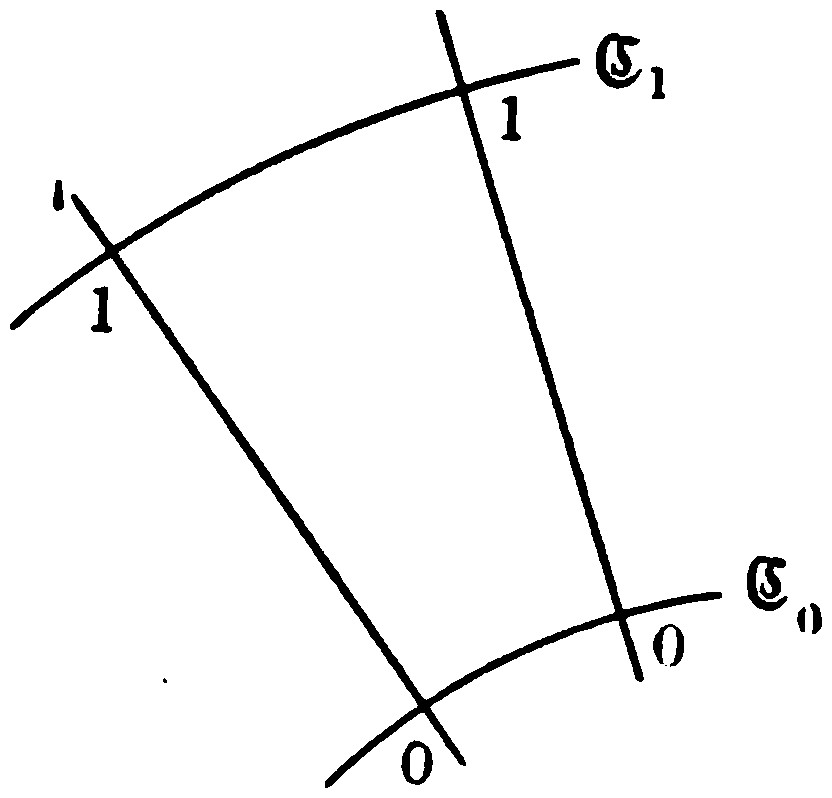
\includegraphics[width=\linewidth,height=32mm,keepaspectratio]{fig_assets/fig01_src_clean_x8.png}
\end{minipage}\hfill
\begin{minipage}[c]{0.49\linewidth}\centering
\end{minipage}
\end{center}

Grenzt man also auf den die Curve $\mathfrak{C}_0$ transversal schneidenden Extremalen des Feldes solche Bögen 01 ab, dass die Integrale $\overline{J}_{01}$ denselben Werth haben, so ist der Ort der Punkte 1 wiederum eine reguläre Curve, welche von den Extremalen des Feldes transversal geschnitten wird. (Vergl. Fig.~1, in welcher, wie auch bei den meisten späteren Figuren, die Extremalen als Gerade erscheinen, die transversale Lage durch rechtwinkeligen Schnitt angedeutet ist.)

Man erkennt in dem erhaltenen Resultat die Verallgemeinerung des bekannten Satzes von \textsc{Gauss}, dass eine Schar gleich langer geodätischer Bögen, welche auf der ihre Anfangspunkte
% src-pdfpage=0071
% src-break=0071
enthaltenden Linie senkrecht stehen, auch den Ort ihrer Endpunkte unter rechtem Winkel schneiden; denn (\S~11) bei den geodätischen Linien fällt die transversale mit der senkrechten Lage zusammen.

\begin{center}{\large \S~16.}\end{center}

Der Integrand $F(x,y,x',y')$ sei regulär und von Null verschieden, etwa positiv, entweder a) in allen der Richtung wachsender $t$ entsprechenden Elementen des Bogens $\mathfrak{B}$, oder b) in allen von Punkten desselben nach beliebigen Richtungen ausgehenden Linienelementen. Diese Eigenschaften behält die Function $F$ im Falle a) für alle Elemente, welche von Punkten des Feldes ausgehen und gegen die bezeichneten Elemente des Bogens $\mathfrak{B}$ hinreichend wenig geneigt sind, im Falle b) für alle von Punkten des Feldes ausgehenden Elemente, vorausgesetzt, dass das Feld hinreichend beschränkt wird. Denn nach \S~3 kann man für jedes einzelne Linienelement annehmen
\[
x'^2+y'^2=1,
\quad x'=\cos\varphi,
\quad y'=\sin\varphi;
\]
dann ist $\varphi$ die im positiven Drehungssinne (\S~4) gemessene Neigung des Elements gegen die $+x$-Axe, und $F$ eine reguläre Function von $x,y,\varphi$, wenn $F(x,y,x',y')$ in dem durch $x,y,\varphi$ charakterisirten Linienelement regulär ist. Hieraus folgt die ausgesprochene Behauptung, da eine an einer Stelle reguläre Function diese Eigenschaft für eine gewisse Umgebung der Stelle behält.

Bei der engeren, wie der weiteren Voraussetzung ist nun
\[
\frac{\partial u}{\partial t}=F(\xi,\eta,\xi_t,\eta_t)
\]
innerhalb des Feldes von Null verschieden; für jedes diesem angehörige Werthsystem $(t,a)$ kann man daher, wenn die Curve $\mathfrak{C}_0$ wie bisher von den Extremalen des Feldes transversal geschnitten wird, aus der Gleichung
\[
u=\int_{t_0}^{t}F(\xi,\eta,\xi_t,\eta_t)dt
\]
die Grösse $t$ und damit auch $x$ und $y$ als reguläre Functionen von $u$ und $a$ berechnen; da die Functionaldeterminante
\[
\frac{\partial(t,a)}{\partial(u,a)}=1:\frac{\partial u}{\partial t}
\]
von Null verschieden ist, so gilt dasselbe von
% src-pdfpage=0072
% src-break=0072
\begin{equation}\tag{36}
\frac{\partial(x,y)}{\partial(u,a)}
=\frac{\partial(\xi,\eta)}{\partial(t,a)}\frac{\partial(t,a)}{\partial(u,a)}
=\Delta:\frac{\partial u}{\partial t}
=\frac{\Delta}{F(\xi,\eta,\xi_t,\eta_t)}.
\end{equation}
Denkt man sich die Ausdrücke von $x$ und $y$ durch $u$ und $a$ in die Function $F(x,y,dx,dy)$ eingeführt, und setzt
\[
v=a,
\quad \frac{dv}{du}=s,
\]
so ergebe sich
\[
F(x,y,dx,dy)=G(u,v,du,dv)=g(u,v,s)du,
\]
\[
J=\int G(u,v,u',v')dt;
\]
dann ist $G$ und nach \S~5 auch, so lange $du$ nicht verschwindet, $g(u,v,s)$ in denselben Linienelementen wie $F$ regulär.

Längs der Extremalen des Feldes ist nun
\[
v=a=\text{const.},\quad s=0,
\]
und da $F$ positiv ist, so wächst $u$ in der Richtung wachsender $t$; man hat also
\[
u=\int_0^1G(u,v,du,0)=\int_0^1g(u,v,0)du,
\]
wobei die Function $g$ einem positiven Werth von $du$ entsprechend zu bilden ist. Differenzirt man nach $u$ und bedenkt, dass 0 als Schnitt der Curve $\mathfrak{C}_0$ und einer Linie $v=\text{const.}$ von $u$ unabhängig ist, so folgt die Identität
\[
1=g(u,v,0),
\]
oder für $du>0$
\[
G(u,v,du,0)=du.
\]

Eine weitere Bestimmung der Function $g$ ergiebt sich, wenn die Thatsache, dass nach \S~15 alle Linien $u=\text{const.}$ von den Extremalen $v=\text{const.}$ transversal geschnitten werden, in den Variablen $u,v$ ausgedrückt wird. Stellen nämlich die Werthsysteme
\[
x,y,x',y';\quad u,v,u',v',
\]
in welchen die Ableitungen nach einem beliebigen Parameter genommen sind, dasselbe Linienelement dar, so gelten die Identitäten
\[
F(x,y,x',y')=G(u,v,u',v'),
\]
\[
x'=x_u u'+x_v v',\quad y'=y_u u'+y_v v',
\]
\[
u'=u_xx'+u_yy',\quad v'=v_xx'+v_yy',
\]
und man kann die erste derselben nach $x'$, $y'$ differenziren; es ergiebt sich dann
% src-pdfpage=0073
% src-break=0073
\[
F_{x'}=G_{u'}\frac{\partial u'}{\partial x'}+G_{v'}\frac{\partial v'}{\partial x'}
=u_xG_{u'}+v_xG_{v'},
\quad F_{y'}=u_yG_{u'}+v_yG_{v'}.
\]
Andererseits hat man für den Fortgang in beliebiger Richtung
\[
Dx=x_uDu+x_vDv,
\quad Dy=y_uDu+y_vDv,
\]
also folgt die Identität
\[
F_{x'}Dx+F_{y'}Dy
=\{G_{u'}(u_xx_u+u_yy_u)+G_{v'}(v_xx_u+v_yy_u)\}Du+\cdots,
\]
oder, da offenbar
\[
\frac{\partial u}{\partial u}=u_xx_u+u_yy_u=1,
\quad
\frac{\partial v}{\partial u}=v_xx_u+v_yy_u=0,
\]
und noch zwei ähnliche Gleichungen bestehen, die Identität
\[
F_{x'}Dx+F_{y'}Dy=G_{u'}Du+G_{v'}Dv.
\]
Diese Grösse verschwindet nach \S~15, wenn $D$ den Fortgang längs der Curve $u=\text{const.}$ bedeutet, die Ableitungen aber sich auf die Extremalen des Feldes beziehen; es muss also die Gleichung
\[
G_{u'}Du+G_{v'}Dv=(g-sg_s)Du+g_sDv=0
\]
durch die Annahme $s=0$, $Du=0$ erfüllt werden, und es ergiebt sich
\[
g_s(u,v,0)=0.
\]
Die Taylor'sche Entwickelung der Function $g$ erhält also, dem gefundenen Werth $g(u,v,0)$ zufolge, wenn $\theta$ der Strecke von 0 bis $+1$ angehört, die Form
\begin{equation}\tag{37}
g(u,v,s)=1+\frac{s^2}{2}g_{ss}(u,v,\theta s).
\end{equation}
Diese Gleichung gilt bei der Voraussetzung a), so lange $|s|$ eine gewisse positive Grösse nicht übersteigt, bei der Voraussetzung b) aber für jeden endlichen Werth von $s$. Offenbar bleibt die bisherige Entwickelung gültig, wenn $\mathfrak{C}_0$ in einen Punkt degenerirt.



\begin{center}
{\small Fig.~2.}\par\vspace{1mm}
\begin{minipage}[c]{0.47\linewidth}\centering
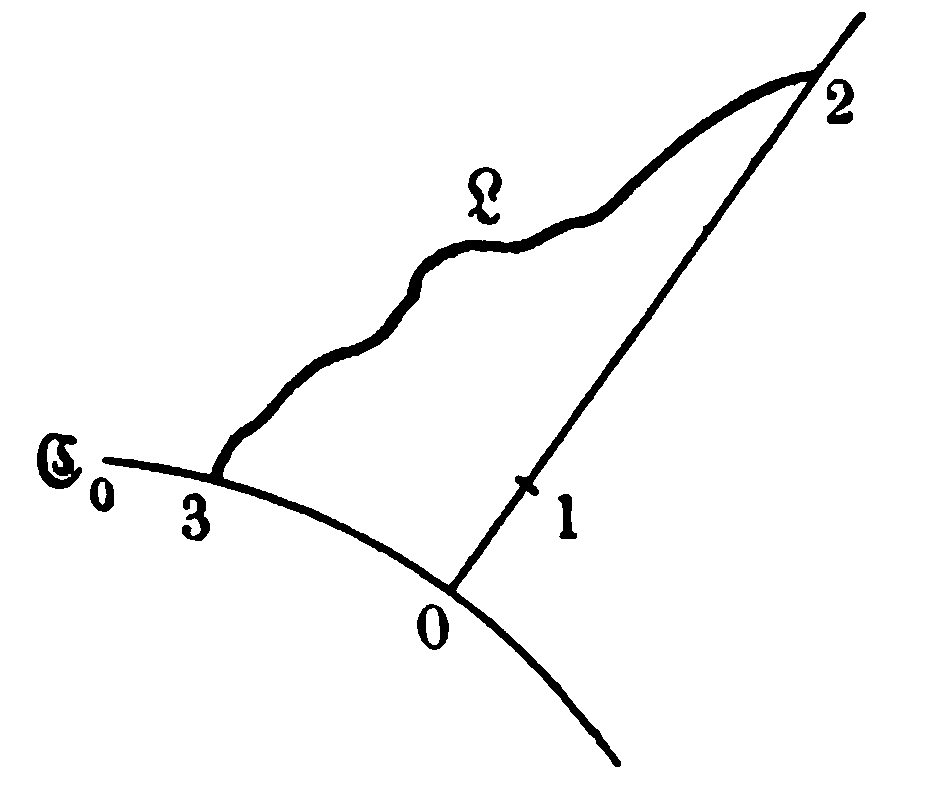
\includegraphics[width=\linewidth,height=32mm,keepaspectratio]{fig_assets/fig02_src_clean_x8.png}
\end{minipage}\hfill
\begin{minipage}[c]{0.49\linewidth}\centering
\end{minipage}
\end{center}

Es sei nun (Fig.~2) 12 irgend ein dem Felde angehöriger Bogen $\mathfrak{B}$, 0 wie bisher der Schnittpunkt der ihn enthaltenden Extremale $\mathfrak{E}$ mit $\mathfrak{C}_0$, 3 ein fester Punkt der letzteren Curve, welcher mit 2 durch eine Curve $\Omega$ verbunden sei. Diese verlasse das Feld nicht; längs ihrer seien $x,y$ solche Functionen eines in der Integrationsrichtung wachsenden Parameters $\tau$, dass das Integral
% src-pdfpage=0074
% src-break=0074
\[
J_{32}=\int_{\tau_3}^{\tau_2}F\left(x,y,\frac{dx}{d\tau},\frac{dy}{d\tau}\right)d\tau
=\int_{\tau_3}^{\tau_2}G\left(u,v,\frac{du}{d\tau},\frac{dv}{d\tau}\right)d\tau
\]
einen bestimmten endlichen Werth hat, und die Gleichung
\begin{equation}\tag{38}
\int_{\tau_3}^{\tau_2}\frac{du}{d\tau}d\tau
=\left.u\right|_3^2
=\left.u\right|_0^2
\end{equation}
besteht. Alsdann ist offenbar
\begin{equation}\tag{39}
J_{32}-\overline{J}_{02}
=\int_3^2\left[G\left(u,v,\frac{du}{d\tau},\frac{dv}{d\tau}\right)-\frac{du}{d\tau}\right]d\tau;
\end{equation}
sobald $du/d\tau$ positiv ist, kann der Integrand nach (37) geschrieben werden
\begin{equation}\tag{40}
\frac{s^2}{2}g_{ss}(u,v,\theta s)\frac{du}{d\tau};
\end{equation}
ist $du/d\tau$ negativ oder Null, so ist der Integrand, ebenso wie $G$, positiv.

Um über das Vorzeichen dieses Integrals zu entscheiden, braucht man die Function $g$ nicht zu bilden, was oft schwierig wäre, sondern kann von den obigen linearen Beziehungen zwischen $x',y',u',v'$ ausgehen; die zweimalige Anwendung derselben ergiebt
\[
\frac{\partial^2G}{\partial v'^2}=G_{v'v'}=F_{x'x'}x_v^2+2F_{x'y'}x_vy_v+F_{y'y'}y_v^2.
\]
Nun folgt aus der Identität
\[
F=x'F_{x'}+y'F_{y'},
\]
indem man nach $x'$ und $y'$ differenzirt,
\[
x'F_{x'x'}+y'F_{x'y'}=x'F_{y'x'}+y'F_{y'y'}=0;
\]
bedenkt man, dass $x'$ und $y'$ nicht beide verschwinden, so folgt, dass eine der Grössen
\[
F_{x'x'}:y'^2,
\quad F_{y'y'}:x'^2
\]
einen endlichen Werth $F_1(x,y,x',y')$ hat, für welchen die Gleichungen
\[
F_{x'x'}=F_1y'^2,
\quad F_{x'y'}=-x'y'F_1,
\quad F_{y'y'}=x'^2F_1,
\quad F_1dt=\frac{f_{pp}dx}{x'^4}
\]
bestehen. Substituirt man diese Werthe in den Ausdruck $G_{v'v'}$, so ergiebt sich
% src-pdfpage=0075
% src-break=0075
\[
G_{v'v'}=F_1(x_vy'-y_vx')^2,
\]
und da
\[
G=u'g\left(u,v,\frac{v'}{u'}\right),
\]
so folgt für nicht verschwindende $u'$
\[
\frac{g_{ss}(u,v,s)}{u'}=F_1(x_vy'-y_vx')^2,
\]
oder nach den zwischen $x',y'$ und $u',v'$ bestehenden linearen Gleichungen
\[
\frac{g_{ss}(u,v,s)}{u'}=F_1\,(x_vy_u-x_uy_v)^2u'^2,
\]
und die rechts erscheinende Klammer ist nach (36) von Null verschieden.

Es werde nun für jeden der Fälle a) und b) vorausgesetzt, dass $F_1$ ein constantes Vorzeichen habe und nicht verschwinde in eben den Linienelementen, für welche in jedem dieser Fälle $F$ regulär ist. Eine Betrachtung, wie die am Anfang dieses Paragraphen durchgeführte, zeigt, dass die angegebene Eigenschaft von $F_1$ im Falle a) nur für die Elemente des Bogens $\mathfrak{B}$, im Fall b) nur für die von seinen Punkten ausgehenden Elemente vorausgesetzt zu werden braucht. Längs dieses Bogens ist $s=0$; übersteigt also $|s|$ längs der Curve $\Omega$ eine gewisse Constante nicht, so haben bei der Voraussetzung a) die Grössen
\[
g_{ss}(u,v,\theta s),
\quad \int\frac{s^2}{2}g_{ss}(u,v,\theta s)du
\]
dasselbe Vorzeichen wie $F_1$, und $u'$ bleibt stets positiv; die Grösse
\begin{equation}\tag{41}
G\left(u,v,\frac{du}{d\tau},\frac{dv}{d\tau}\right)-\frac{du}{d\tau}
\end{equation}
ist stets in der Form (40) darstellbar und hat ebenfalls das Vorzeichen mit $F_1$ gemein. Sobald dagegen $du/d\tau$ stellenweise aufhört, positiv zu sein, werde die Voraussetzung b) eingeführt; dann gilt für $u'>0$ die Gleichung
\[
G(u,v,u',v')-u'=\frac{s^2}{2}g_{ss}(u,v,\theta s)u'
=\frac{v'^2}{2u'}g_{ss}(u,v,\theta s).
\]
Dreht sich daher das Linienelement $(u,v,u',v')$ um einen festen Punkt und convergirt $u'$ von der positiven Seite her gegen Null, so nähert sich die linke Seite der Grenze $G(u,v,0,v')$ an, während die rechte das Vorzeichen von $F_1$ hat; letzteres muss
% src-pdfpage=0076
% src-break=0076
also mit dem des Integranden $G$ oder $F$, welchen wir als positiv voraussetzen, übereinstimmen, d.~h. auch $F_1$ ist positiv. Die Grösse (41) ist also bei positiven Werthen $du/d\tau$ positiv und verschwindet nur für $s=0$; bei negativen oder verschwindenden Werthen $du/d\tau$ ist sie offenbar positiv. Dasselbe gilt daher von der Differenz $J_{32}-\overline{J}_{02}$, sobald die Gleichung (38) richtig ist und die Integraldarstellung (39) einen Sinn hat.

\begin{center}{\large \S~17.}\end{center}

Der Begriff des Extremums muss genauer bestimmt werden durch Angaben über die Gesammtheit aller derjenigen Curven, welche man zum Vergleich heranziehen will. Die allgemeine Vorstellung eines Extremums bringt es mit sich, dass man zunächst benachbarte Curven vergleicht; für die Nachbarschaft führen wir folgende Definitionen ein. Ist 12 irgend ein ebener Bogen, und liegt der Bogen $\Omega$ ganz im Inneren derjenigen Fläche, welche von einem Kreise mit constantem Radius $\rho$ bedeckt wird, dessen Mittelpunkt den Bogen 12 durchläuft, so sagen wir, alle Curven $\Omega$, für welche die zugehörigen Grössen $\rho$ eine gewisse Constante nicht übersteigen, gehören einer weiteren Nachbarschaft des Bogens 12 an. Giebt es noch eine positive Constante $\rho_1$ von der Beschaffenheit, dass jede Tangente des Bogens $\Omega$ mit mindestens einer des Bogens 12, deren Berührungspunkt von dem der ersteren um weniger als $\rho$ entfernt ist, einen Winkel bildet, der kleiner als $\rho_1$ ist, so sagen wir, der Bogen $\Omega$ liege in engerer Nachbarschaft des Bogens 12, sobald $\rho$ und $\rho_1$ unterhalb gewisser Constanten verbleiben. Diese Definitionen können offenbar auf Raumcurven sofort übertragen werden. Ist ferner die Differenz der längs beider Bögen gebildeten Integrale $J$ von constantem Vorzeichen, sobald $\Omega$ in einer weiteren Nachbarschaft des Bogens 12 liegt, so sagen wir, der Bogen 12 ergebe ein starkes Extremum des Integrals $J$. Hat dagegen jene Differenz ein festes Vorzeichen nur dann, wenn $\Omega$ in einer engeren Nachbarschaft von 12 liegt, so sagen wir, es finde ein schwaches Extremum statt. Im letzteren Falle ist zum Vergleich mit dem Bogen 12 offenbar ein engeres Gebiet von Curven $\Omega$ herangezogen worden, als im ersten.

Um aber ein Extremum nachweisen zu können, müssen wir für die Curven $\Omega$ gewisse Stetigkeitseigenschaften voraussetzen,
% src-pdfpage=0077
% src-break=0077
die im Wesentlichen darauf hinauslaufen, dass längs dieser Curven Integrale von der Form $J$ gebildet und nach den gewöhnlichen Operationsregeln der Infinitesimalrechnung behandelt werden können. Um solche Eigenschaften genau formuliren zu können, betrachten wir im Allgemeinen eine Function $\varphi(\tau)$, welche in einem beliebig begrenzten Intervall $\mathfrak{J}$ folgende Eigenschaften hat. Sie sei stetig und der Quotient
\[
\frac{\varphi(\tau+\varepsilon)-\varphi(\tau)}{\varepsilon}
\]
nähere sich, wenn $\varepsilon$ positiv ist und unendlich abnimmt, für jeden Werth von $\tau$ einer bestimmten endlichen Grenze $\varphi'(\tau)$. Dabei braucht nicht ausgeschlossen zu werden, dass der Quotient
\[
\frac{\varphi(\tau-\varepsilon)-\varphi(\tau)}{-\varepsilon}
\]
sich einer anderen oder gar keiner Grenze annähert. Die Grösse $\varphi'(\tau)$ nennen wir, wie es bisweilen geschehen ist, die vordere Ableitung. Es gilt auch für sie, ebenso wie für den gewöhnlichen Begriff der Ableitung der Satz, dass die stetige Function $\varphi(\tau)$ in dem Intervall von $\tau_0$ bis $\tau_1$ constant sein muss, wenn die vordere Ableitung in dieser Strecke überall den bestimmten Werth Null hat; denn setzt man
\[
\psi(\tau)=\varphi(\tau)+\alpha(\tau-\tau_0),
\quad \theta(\tau)=\varphi(\tau)-\alpha(\tau-\tau_0)
\]
und versteht unter $\alpha$ eine positive Constante, so hat $\psi(\tau)$ die vordere Ableitung $\alpha$, $\theta(\tau)$ die vordere Ableitung $-\alpha$; erstere Function wächst daher, letztere nimmt ab zwischen $\tau_0$ und $\tau_1$, so dass, wenn $\tau_1>\tau_0$ ist, die Ungleichungen
\[
\psi(\tau_1)>\psi(\tau_0),
\quad \theta(\tau_1)<\theta(\tau_0),
\]
\[
\varphi(\tau_1)+\alpha(\tau_1-\tau_0)>\varphi(\tau_0),
\quad \varphi(\tau_1)-\alpha(\tau_1-\tau_0)<\varphi(\tau_0),
\]
\[
\alpha(\tau_1-\tau_0)>\varphi(\tau_0)-\varphi(\tau_1)>-\alpha(\tau_1-\tau_0)
\]
bestehen. Die letzte von ihnen ergiebt, da $\alpha$ beliebig klein sein kann, $\varphi(\tau_1)=\varphi(\tau_0)$, womit die Behauptung bewiesen ist.

Von diesem Specialfalle abgesehen, habe nun die Function $\varphi'(\tau)$ folgende Eigenschaft. Ihre Schwankung in irgend einem Intervall sei die obere Grenze der absolut genommenen Differenzen irgend zweier in diesem Intervall erreichter Werthe der Function; die Gesammtlänge aller Theile des Intervalls $\mathfrak{J}$, innerhalb deren die Schwankung von $\varphi'(\tau)$ eine positive Constante übersteigt,
% src-pdfpage=0078
% src-break=0078
könne stets unendlich klein gemacht werden. Alsdann ist nach \textsc{Riemann} die Function $\varphi'(\tau)$ integrabel, und das Integral
\[
\Phi(\tau)=\int_{\tau_0}^{\tau}\varphi'(\tau)d\tau,
\]
dessen Integrationsintervall einen Theil von $\mathfrak{J}$ bilde, ist eine endliche, stetige Function von $\tau$. Weiter setzen wir voraus, es sei, wenn $\varepsilon$ positiv ist
\[
\lim_{\varepsilon=0}\varphi'(\tau+\varepsilon)=\varphi'(\tau);
\]
dadurch werden die Unstetigkeiten der Function $\varphi'(\tau)$ in gewisser Weise beschränkt, es ist aber z.~B. immer noch möglich, dass in beliebiger Nähe einer Unstetigkeitsstelle unendlich viele andere liegen. Bei dieser Voraussetzung ist die Grösse $\varphi'(\tau)$ längs einer endlichen Strecke positiv, wenn dies für eine einzige Stelle gilt. Man erhält ferner für $\varepsilon>0$
\[
\Phi(\tau+\varepsilon)-\Phi(\tau)
=\int_{\tau}^{\tau+\varepsilon}\varphi'(\tau)d\tau=M\varepsilon,
\]
wobei $M$ zwischen der oberen und unteren Grenze der Werthe liegt, welche $\varphi'(\tau)$ zwischen $\tau$ und $\tau+\varepsilon$ annimmt; nach der vorigen Gleichung convergirt $M$ gegen $\varphi'(\tau)$, wenn $\varepsilon$ verschwindet. Die Grösse $\Phi(\tau)$ hat also die vordere Ableitung
\[
\Phi'(\tau)=\varphi'(\tau),
\]
die Differenz $\Phi(\tau)-\varphi(\tau)$ ist constant, und da $\Phi(\tau_0)$ verschwindet, ergiebt sich
\[
\Phi(\tau)=\varphi(\tau)-\varphi(\tau_0)=\int_{\tau_0}^{\tau}\varphi'(\tau)d\tau.
\]
Es gilt somit die gewöhnliche Fundamentalbeziehung zwischen Differentiation und Integration, wenn man erstere Operation auf die vorderen Ableitungen bezieht.

Jetzt seien $x$ und $y$ längs der Curve $\Omega$ Functionen des Parameters $\tau$, welche die Eigenschaften der Function $\varphi(\tau)$ haben, also integrirbare, vordere Ableitungen besitzen, die wir durch die gewöhnlichen Differentialsymbole bezeichnen; dabei liege die Summe
\[
\left(\frac{dx}{d\tau}\right)^2+
\left(\frac{dy}{d\tau}\right)^2
\]
stets oberhalb einer positiven Constante. Hiermit ist, da $\varphi'(\tau)$ nicht stetig zu sein braucht, keineswegs ausgeschlossen, dass die
% src-pdfpage=0079
% src-break=0079
Curve $\Omega$ Ecken in endlicher oder unendlicher Menge besitzt; sie hat aber in jedem Punkte eine bestimmte, den wachsenden Werthen von $\tau$ entsprechende Richtung. Liegt $\Omega$ in einer hinreichend begrenzten, engeren oder weiteren Nachbarschaft des Bogens $\mathfrak{B}$, je nachdem die Voraussetzung a) oder b) des vorigen Paragraphen gilt, so weicht im ersten Falle jedes Werthsystem
\[
\left(x,y,\frac{dx}{d\tau},\frac{dy}{d\tau}\right)
\]
beliebig wenig von einem solchen ab, welches ein Element der Curve $\mathfrak{E}$ darstellt; im zweiten Falle ist $F$ für beliebig gerichtete, von Punkten des Feldes ausgehende Linienelemente regulär; in beiden Fällen gilt dies daher für jedes durch die Curve $\Omega$ definirte Werthsystem
\[
\left(x,y,\frac{dx}{d\tau},\frac{dy}{d\tau}\right),
\]
und die einem veränderlichen Intervall des Arguments $\tau$ entsprechende Schwankung der Grösse
\[
F\left(x,y,\frac{dx}{d\tau},\frac{dy}{d\tau}\right)
\]
wird mit der in demselben Intervall vorhandenen Schwankung der Grössen
\[
\frac{dx}{d\tau},\quad \frac{dy}{d\tau}
\]
unendlich klein. Setzen wir ferner
\[
F\left(x,y,\frac{dx}{d\tau},\frac{dy}{d\tau}\right)=\Theta(\tau),
\]
so ist offenbar, wenn $\varepsilon>0$,
\[
\Theta(\tau)=\lim_{\varepsilon=0}\Theta(\tau+\varepsilon),
\]
da eine solche Gleichung für $dx/d\tau$ und $dy/d\tau$ gilt; $\Theta(\tau)$ hat also alle oben vorausgesetzten Eigenschaften von $\varphi'(\tau)$, ist integrirbar und ergiebt die Gleichung
\[
\frac{d}{d\tau}\int_{\tau_0}^{\tau}\Theta(\tau)d\tau
=\frac{d}{d\tau}\int_{\tau_0}^{\tau}F\left(x,y,\frac{dx}{d\tau},\frac{dy}{d\tau}\right)
=F\left(x,y,\frac{dx}{d\tau},\frac{dy}{d\tau}\right),
\]
welche den gewöhnlichen Regeln der Integralrechnung entspricht. Dieselben Eigenschaften wie $F$ hat, wenn $\Phi(x,y)$ eine längs der Curve $\Omega$ reguläre Function der Coordinaten ist, die Grösse
\[
\frac{d\Phi}{d\tau}=\Phi_x\frac{dx}{d\tau}+\Phi_y\frac{dy}{d\tau};
\]
wendet man diese Bemerkungen auf die Grössen $u,v$ an, welche reguläre Functionen der Coordinaten sind, so folgt, dass auch die Grössen
% src-pdfpage=0080
% src-break=0080
\[
G\left(u,v,\frac{du}{d\tau},\frac{dv}{d\tau}\right),
\quad \frac{du}{d\tau},\quad \frac{dv}{d\tau}
\]
die Eigenschaften von $\varphi'(\tau)$ haben und speciell die Differenz der ersten beiden Grössen längs einer endlichen Strecke positiv ist, wenn dies für eine einzige Stelle eintritt. Ferner folgt, dass die Gleichungen (38), (39) bei den eingeführten Voraussetzungen richtig sind, wenn wir das Zeichen der Differentiation nach $\tau$ stets auf die vorderen Ableitungen beziehen. Das ist bei der Bildung von $J_{32}$ ganz naturgemäss, da in der Richtung wachsender $\tau$ integrirt wird.

Auf Grund dieser Entwickelungen ist jetzt streng zu erweisen, dass die Grösse
\[
J_{32}-\overline{J}_{02}
=\int_3^2\left[G\left(u,v,\frac{du}{d\tau},\frac{dv}{d\tau}\right)-\frac{du}{d\tau}\right]d\tau
\]
das Vorzeichen mit $F_1$ gemein hat und nur dann verschwindet, wenn die Curven $\Omega$ und $\mathfrak{B}$ völlig zusammenfallen. Dies ist im Falle a) ohne Weiteres klar, da der Integrand längs des ganzen Integrationsintervalls durch
\begin{equation}\tag{42}
\frac{s^2}{2}g_{ss}(u,v,\theta s)\frac{du}{d\tau}
\end{equation}
ersetzt werden kann, die Grösse $g_{ss}du$ aber nach Voraussetzung nicht verschwindet. Im Falle b) ist der Integrand ebenfalls nie negativ, und kann, wenn $J_{32}-\overline{J}_{02}$ verschwinden soll, die Grösse $dv/d\tau$ jedenfalls da nicht von Null verschieden sein, wo $du/d\tau$ positiv ist; denn in diesem Falle ist der Integrand wiederum in der Form (42) darstellbar, also positiv. Wird aber $du/d\tau$ an einer Stelle negativ, so ist der Integrand des obigen Integrals wiederum positiv; da derselbe nun, wie oben bemerkt, längs einer endlichen Strecke positiv bleibt, wenn dies an einer einzigen Stelle eintritt, so kann das Integral $J_{32}-\overline{J}_{02}$ sicher nur verschwinden, wenn $v$ längs der Curve $\Omega$ constant ist, letztere also mit $\mathfrak{B}$ zusammenfällt.

Damit ist der Nachweis des Extremums vollendet, gleichviel, ob man den Bogen 02 mit allen Bögen, welche dieselben Endpunkte haben, oder mit allen von der Curve $\mathfrak{C}_0$ nach dem Punkte 2 gehenden, vergleicht. Zieht sich jedoch die Curve $\mathfrak{C}_0$ in
% src-pdfpage=0081
% src-break=0081
den Punkt 0 zusammen, so dass durch ihn alle Extremalen des Feldes gehen, so muss für die Curve $\Omega$ noch besonders vorausgesetzt werden, dass sie immer innerhalb des von den Extremalen des Feldes einfach bedeckten Gebietes verbleibe (Fig.~3). Dies erreicht man z.~B. dadurch, dass man alle Curven $\Omega$ ein beliebig kleines, constantes Stück 01 mit der Curve $\mathfrak{E}$ gemein haben lässt (Fig.~4); dann ist



\begin{center}
\begin{minipage}[c]{0.47\linewidth}\centering
{\small Fig.~3.}\par\vspace{1mm}
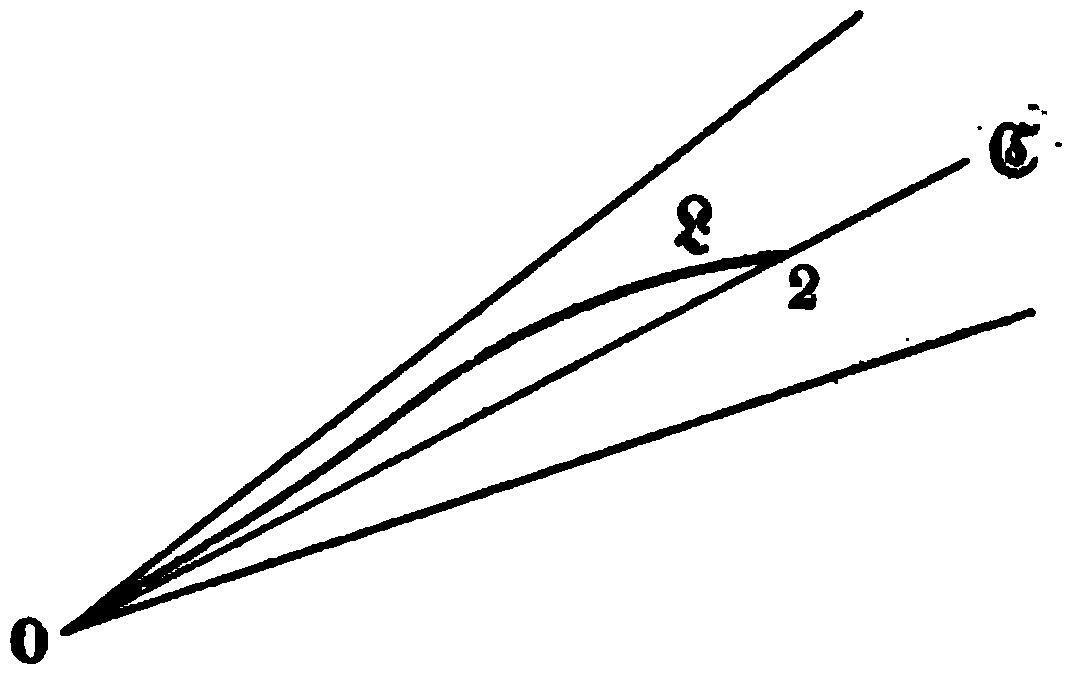
\includegraphics[width=\linewidth,height=24mm,keepaspectratio]{fig_assets/fig03_src_clean_x8.png}\par\vspace{1mm}
\end{minipage}\hfill
\begin{minipage}[c]{0.47\linewidth}\centering
{\small Fig.~4.}\par\vspace{1mm}
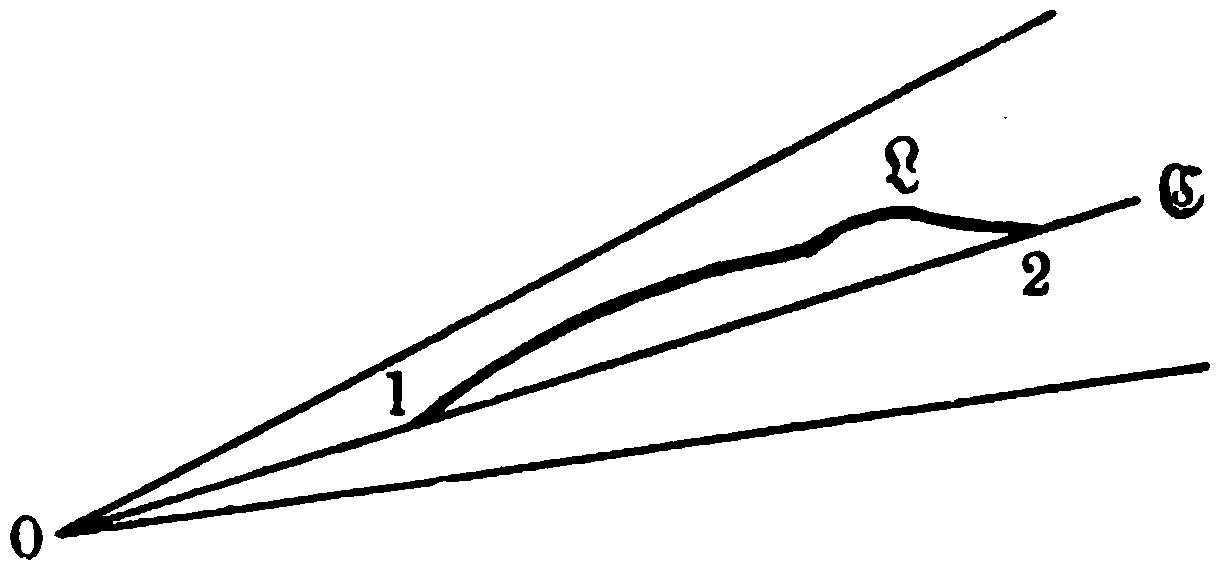
\includegraphics[width=\linewidth,height=24mm,keepaspectratio]{fig_assets/fig04_src_clean_x8.png}\par\vspace{1mm}
\end{minipage}
\end{center}
\[
J_{32}-\overline{J}_{02}=J_{02}-\overline{J}_{02}=\overline{J}_{01}+J_{12}-\overline{J}_{02}=J_{12}-\overline{J}_{12},
\]
und für den Bogen 12 ist das Extremum gegenüber allen Bögen mit denselben Endpunkten im unbeschränkten Sinne der obigen Definition gesichert. Dies gilt auch, wenn die Extremalen im Punkte 0 singulär werden, dabei aber die in \S~15 für diesen Fall ausgesprochenen Voraussetzungen gelten. Endlich übersieht man leicht, dass die Argumentation nicht geändert wird, wenn der Punkt 2 als Endpunkt des Bogens $\Omega$ auf einer Curve $\mathfrak{C}_2$, welche die Extremalen des Feldes transversal schneiden, veränderlich gelassen wird, während 0 festgehalten wird, so dass die Integrationsrichtung, entgegen der bisherigen Annahme, vom festen Punkte zur festen Curve hinführt.

Die Ausdehnung des Feldes, innerhalb dessen die Curven $\Omega$ verlaufen müssen, haben wir in \S~16 so beschränkt, dass die Voraussetzungen a), b) von Punkten oder Elementen des Bogens $\mathfrak{E}$ auf alle Extremalen des Feldes übertragen werden können, ebenso in \S~15, um zu erreichen, dass die Curven $u=\text{const.}$ regulär bleiben und jede der Extremalen des Feldes nur einmal schneiden. Wenn diese durch Beschränkung des Feldes stets zu erreichenden Eigenschaften in einer speciellen Aufgabe für ein bestimmtes Feld von endlicher Ausdehnung nachweisbar sind, so gilt unsere Argumentation für jede in diesem Felde verlaufende Curve $\Omega$, und liefert dann mehr als den Nachweis des Extremums; denn letzteres ist schon gesichert, wenn nur ein Feld von beliebig kleiner Ausdehnung construirt ist.
% src-pdfpage=0082
% src-break=0082

Die wichtigsten der erhaltenen Resultate fassen wir in folgender Weise zusammen. 1. \textsc{Jacobi}'sche Bedingung. Ein nirgends singuläres Stück einer Extremale mit den Endpunkten 0, 2 sei mit einem Felde umgeben. 2. \textsc{Legendre}'sche Bedingung. Entweder a) in allen Elementen des Bogens 02, der in der Richtung von 0 nach 2 hin durchlaufen werde, oder b) in allen von Punkten desselben ausgehenden Linienelementen habe die Grösse $F_1$ oder $f_{pp}dx$ ein festes Vorzeichen, ohne zu verschwinden, und $F$ sei regulär und von Null verschieden. Dann liefert der Bogen 02 ein Extremum des Integrals $J$, sowohl im Vergleich zu allen Curven $\Omega$ mit denselben Endpunkten, als auch zu allen, welche die vom Punkte 0 ausgehende, von den Extremalen des Feldes transversal durchschnittene Curve $\mathfrak{C}_0$ mit dem Punkte 2 verbinden. Das starke oder schwache Extremum ist gesichert, je nachdem die Voraussetzung b) oder a) gemacht wird; ein Maximum oder Minimum tritt ein, je nachdem $F_1$ negativ oder positiv ist.

% src-pdfpage=0082
% src-break=0082
\begin{center}{\large \S~18.}\end{center}

\noindent\textbf{Beispiele. Aufgabe I (\S~9).} Man hat hier
\[
Fdt=\sqrt{x'^2+y'^2}\,dt,
\]
die Quadratwurzel ist positiv, also
\[
y'^2F_1=F_{x'x'}=\frac{\partial}{\partial x'}
\left(\frac{x'}{\sqrt{x'^2+y'^2}}\right)
=\frac{y'^2}{\left(\sqrt{x'^2+y'^2}\right)^3},
\]
\[
F_1=\left(\frac{1}{\sqrt{x'^2+y'^2}}\right)^3
\]
mit ebenfalls positiver Quadratwurzel. Ferner ist
\[
Fdt=f\,dx,\quad f=\sqrt{1+p^2},\quad
f_{pp}=\left(\frac{1}{\sqrt{1+p^2}}\right)^3,
\]
wobei die Quadratwurzel das Vorzeichen von $dx$ hat, so dass für jedes Bogenelement $f_{pp}dx$ ebenso wie $F_1$ positiv ist. Die \textsc{Legendre}'sche Vorzeichenbedingung des starken Minimums ist also erfüllt.

Um zu untersuchen, ob eine gerade Strecke 12 die kürzeste Linie zwischen 1 und 2 liefert, nehmen wir an (Fig.~5), $\Omega$ sei irgend eine Linie 12 von den in \S~17 angegebenen Stetigkeitseigenschaften, welche das Bogenintegral $J_{12}$ ergiebt; die Länge
% src-pdfpage=0083
% src-break=0083
der Strecke 12 ist $\overline{J}_{12}$. Es sei ferner 0 ein Punkt der Geraden 12, der nicht der Linie $\Omega$ angehört und ausserhalb der Strecke 12 liegt; man nehme ihn zum Anfangspunkt der rechtwinkeligen und der Polarcoordinaten, indem man setzt
\[
x=t\cos v,\quad y=t\sin v
\]
und wähle die Constanten $\alpha,\beta$ so, dass
\[
0<\alpha<\beta
\]
und die Curve $\Omega$ ganz im Inneren der Ringfläche zwischen den Kreisen $t=\alpha$, $t=\beta$ verläuft. Diese Fläche, welche von den Extremalen $v=\text{const.}$ genau einfach bedeckt wird, kann als Feld der geraden Strecke 12 betrachtet werden, da in ihr die Grösse
\[
\frac{\partial(x,y)}{\partial(t,v)}
=
\begin{vmatrix}
\cos v & \sin v\\
-t\sin v & t\cos v
\end{vmatrix}
=t
\]
von Null verschieden ist.



\begin{center}
{\small Fig.~5.}\par\vspace{1mm}
\begin{minipage}[c]{0.47\linewidth}\centering
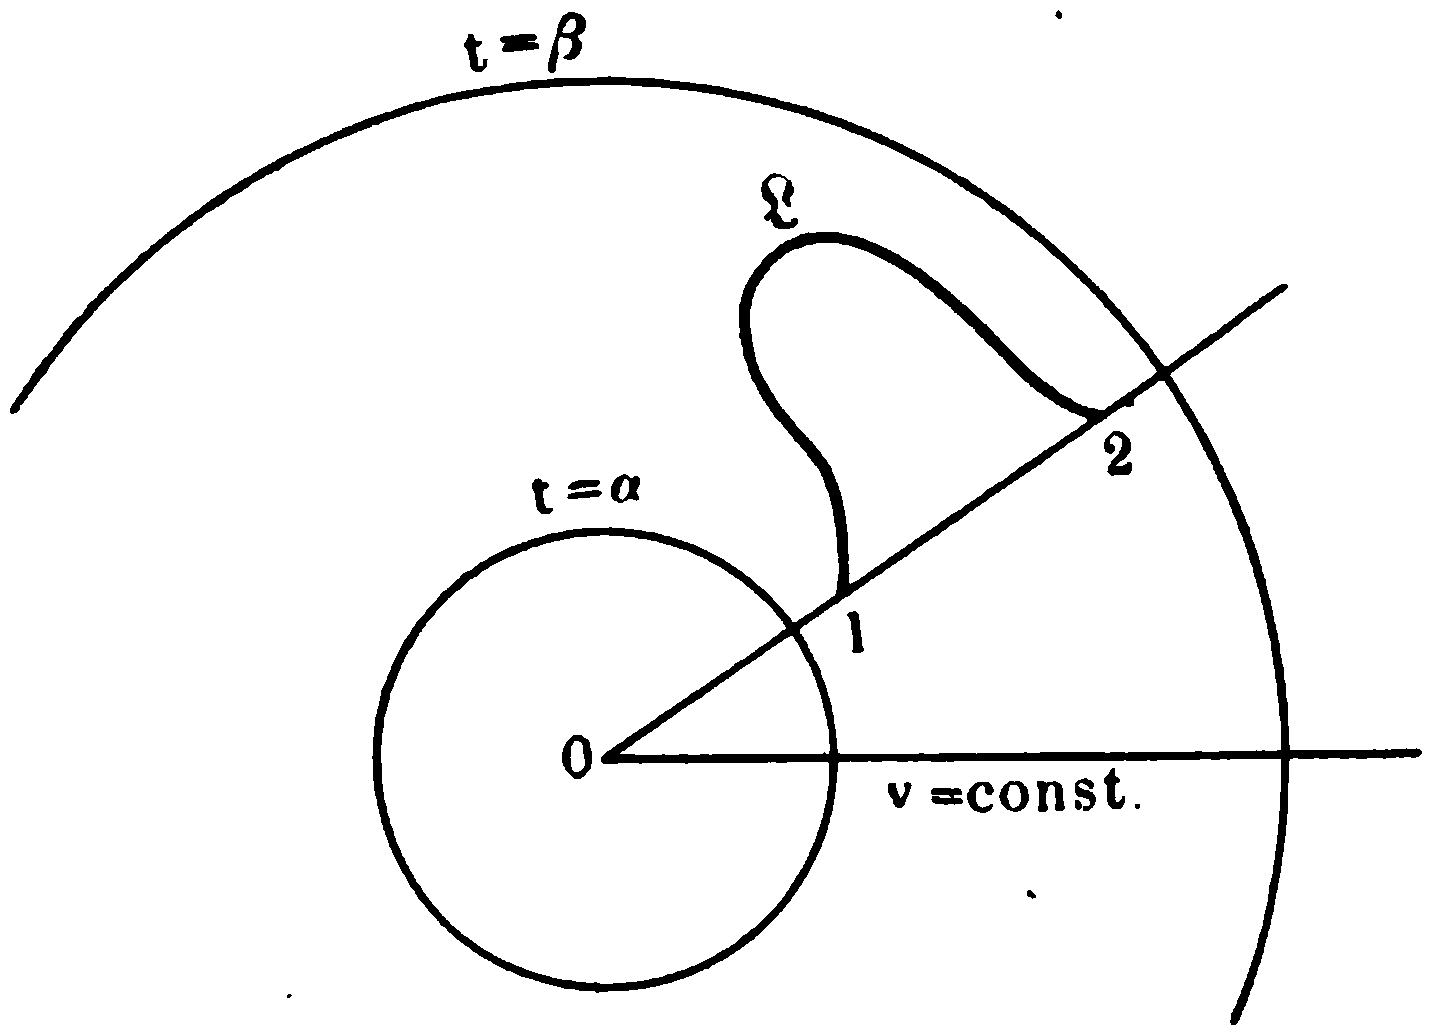
\includegraphics[width=\linewidth,height=32mm,keepaspectratio]{fig_assets/fig05_src_clean_x8.png}
\end{minipage}\hfill
\begin{minipage}[c]{0.49\linewidth}\centering
\end{minipage}
\end{center}

Den Curven $\mathfrak{C}_0$ der allgemeinen Theorie entsprechen die Kreise $t=\text{const.}$, deren jeder die Extremalen des Feldes in je einem Punkte schneidet; $u$ ist die Länge einer Geraden $v=\text{const.}$ vom Kreise $t=\alpha$ an gemessen, somit folgt
\[
u+\alpha=t,\quad
Fdt=\sqrt{dt^2+t^2dv^2}=\sqrt{du^2+(u+\alpha)^2dv^2}
=G(u,v,du,dv),
\]
\[
g(u,v,s)=\sqrt{1+(u+\alpha)^2s^2},
\]
wobei auch die letzte Quadratwurzel positiv ist, da der Ausdruck $g$ nur für den Fall $du>0$ gebildet wird. In der Differenz
\[
J_{12}-\overline{J}_{12}
=
\int_{\tau_1}^{\tau_2}
\left[
G\left(u,v,\frac{du}{d\tau},\frac{dv}{d\tau}\right)
-\frac{du}{d\tau}
\right]d\tau
\]
ist der Integrand von selbst positiv, sobald $\frac{du}{d\tau}$ negativ ist oder verschwindet, was die Theile der Curve $\Omega$ charakterisiert, in welchen der Radius $t$ abnimmt. Ist $\frac{du}{d\tau}$ positiv, so kann der Integrand geschrieben werden
% src-pdfpage=0084
% src-break=0084
\[
\sqrt{1+(u+\alpha)^2s^2}-1,
\]
ist also ebenfalls nicht negativ und verschwindet nur für $s=0$. Wäre an irgend einer Stelle $s$ von Null verschieden oder der Integrand positiv, so würde nach \S~17 dasselbe für eine endliche Strecke der Curve $\Omega$ gelten, die Differenz $J_{12}-\overline{J}_{12}$ könnte also nur verschwinden, wenn überall $du$ positiv und $s=0$ wäre. Von diesem Falle abgesehen, hat man offenbar
\[
J_{12}>\overline{J}_{12},
\]
womit das starke Minimum nachgewiesen ist, und noch mehr.

Weiter sei $\mathfrak{C}_1$ irgend eine vom Punkte 1 durchlaufene Curve, so dass $x_1,y_1$ reguläre Functionen eines Parameters $v$ sind, $n$ die Richtung der Normalen, welche zur Richtung wachsender $v$ so liegt, wie die $+y$-Axe zur $+x$-Axe; setzen wir dann
\[
x=\xi(t,v)=x_1+t\cos(nx),\quad
y=\eta(t,v)=y_1+t\cos(ny),
\]
so ist $v=\text{const.}$ eine Normale der Curve $\mathfrak{C}_1$, und man hat
\[
\Delta=\frac{\partial(\xi,\eta)}{\partial(t,v)}
=
\begin{vmatrix}
\cos(nx) & \dfrac{dx_1}{dv}+t\,\dfrac{d\cos(nx)}{dv}\\[1.1em]
\cos(ny) & \dfrac{dy_1}{dv}+t\,\dfrac{d\cos(ny)}{dv}
\end{vmatrix}.
\]
Ist speciell $v$ die Bogenlänge auf der Curve $\mathfrak{C}_1$, so hat man
\[
\cos(nx)=-\frac{dy_1}{dv},\quad \cos(ny)=\frac{dx_1}{dv},
\]
\[
\Delta=-1+t\left(
\frac{dx_1}{dv}\frac{d^2y_1}{dv^2}
-\frac{dy_1}{dv}\frac{d^2x_1}{dv^2}
\right)
=-1+\frac{t}{r},
\]
wobei $r$ den Krümmungsradius im Punkte 1 bedeutet, positiv oder negativ genommen, je nachdem der Krümmungsmittelpunkt nach der Richtung $n$ oder der entgegengesetzten hin liegt.

Nun stimme auf irgend einer Normalen $v=\text{const.}$ die Richtung von 1 nach dem Punkte 2 hin mit $n$ überein, so dass $t_2$ positiv ist; dann lässt sich die gerade Strecke 12, deren Länge $t_2$ ist, mit einem Felde umgeben, in welchem $\Delta$ nicht verschwindet, wenn entweder $r$ negativ ist oder die Ungleichung
\[
0<t_2<r
\]
besteht, d. h. immer, wenn die Strecke 12 den Krümmungsmittelpunkt des Punktes 1 nicht enthält (Fig.~6). Die Extremalen
% src-pdfpage=0085
% src-break=0085
 des Feldes sind die Normalen $v=\text{const.}$, welche die Curve $\mathfrak{C}_1$ transversal schneiden. Die allgemeine Theorie ergiebt also, dass die gerade Strecke 12 ein starkes Minimum der Entfernung zwischen $\mathfrak{C}_1$ und dem Punkte 2 liefert, und kürzer ist als jede im Felde verlaufende Linie $\Omega$ von den oben angegebenen Stetigkeitseigenschaften, welche von der Curve $\mathfrak{C}_1$ zum Punkte 2 führt. Die Grösse $u$ ist der normale Abstand von der Curve $\mathfrak{C}_1$; und man erhält leicht die Formel



\begin{center}
{\small Fig.~6.}\par\vspace{1mm}
\begin{minipage}[c]{0.47\linewidth}\centering
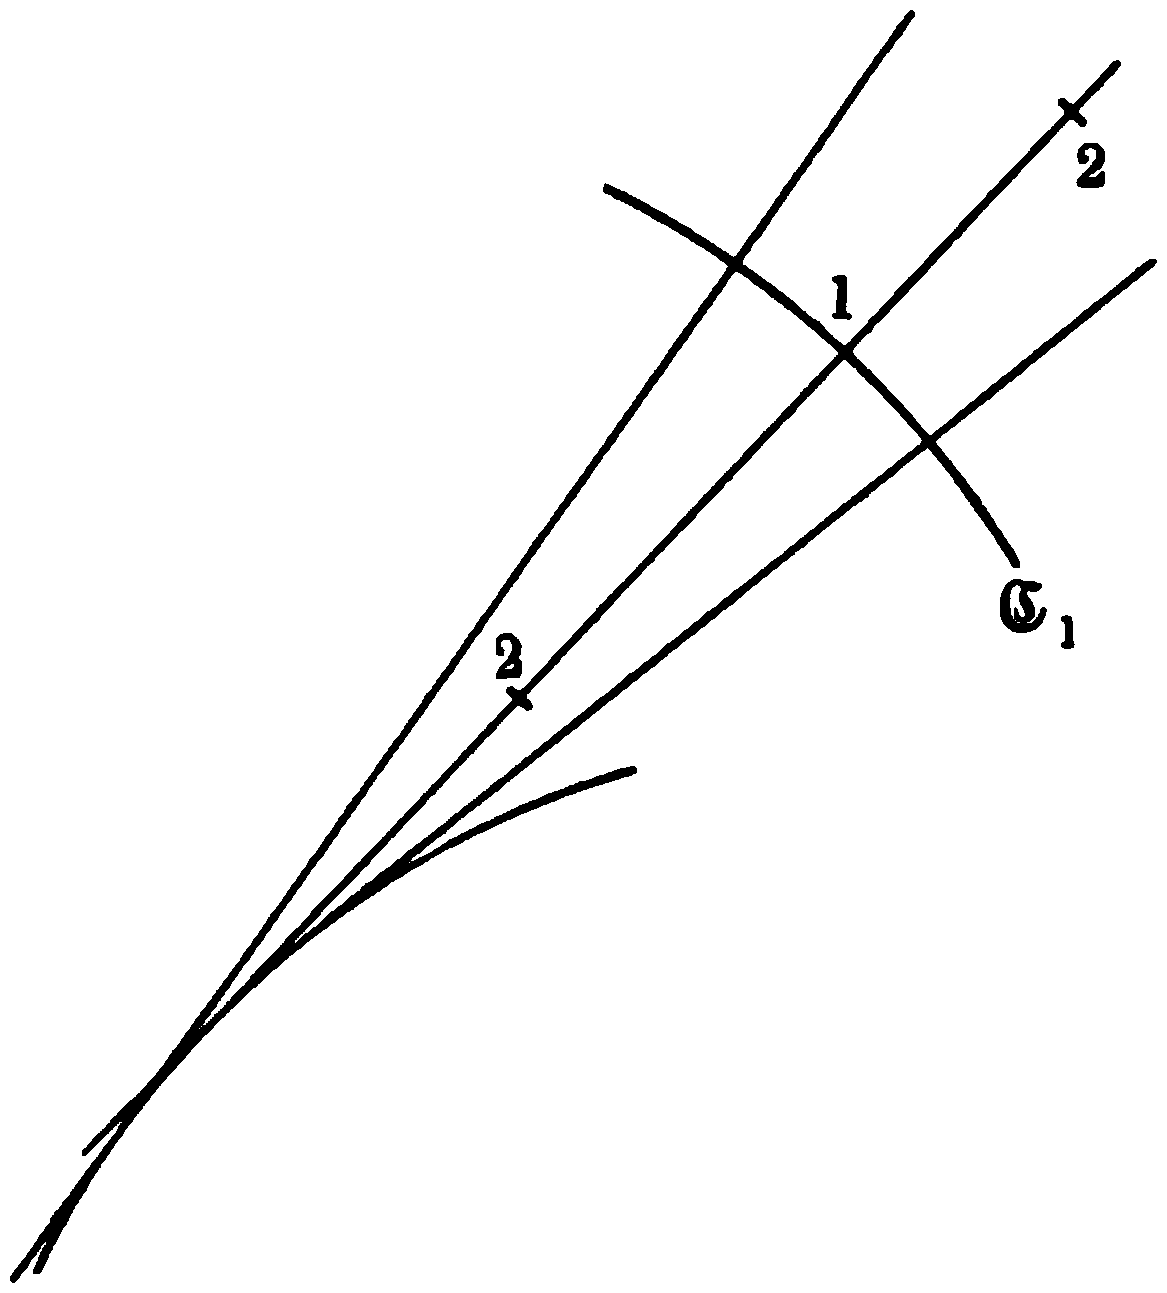
\includegraphics[width=\linewidth,height=32mm,keepaspectratio]{fig_assets/fig06_src_clean_x8.png}
\end{minipage}\hfill
\begin{minipage}[c]{0.49\linewidth}\centering
\end{minipage}
\end{center}

\[
\sqrt{dx^2+dy^2}
=
\sqrt{du^2+(u-r)^2dv^2}
=G(u,v,du,dv),
\]
an welche sich dieselben Schlüsse knüpfen lassen wie an die frühere Transformation des Bogenelementes.

\bigskip

\noindent\textbf{Aufgabe III (\S~9).} Ist in der $wy$-Ebene $\Omega$ irgend eine vom Punkte 0 in der Halbebene $y>0$ zur $w$-Axe gezogene Linie von der Länge $l$, längs deren $w,y$ als Functionen eines Parameters $\tau$ die Eigenschaften von $\varphi(\tau)$ (\S~17) haben, so ist nachzuweisen, dass das Flächenintegral kleiner ist als die Fläche des Halbkreises von der Länge $l$. Wenn $\frac{dw}{d\tau}$ streckenweise negativ ist, so betrachten wir die Curve $\Omega^0$, welche durch die Gleichungen
\[
y=\int_{\tau_0}^{\tau}\frac{dy}{d\tau}\,d\tau,\quad
w=\int_{\tau_0}^{\tau}\left|\frac{dw}{d\tau}\right|\,d\tau
\]
definirt ist; diese hat, wenn $\tau$ dasselbe Intervall wie auf der Curve $\Omega$ durchläuft, ebenfalls die Länge $l$ und dieselben Stetigkeitseigenschaften, da, wie man leicht sieht, $|\varphi(\tau)|$ die in \S~17 für $\varphi(\tau)$ geforderten Eigenschaften ebenfalls besitzt. Das Flächenintegral der Curve $\Omega^0$ ist endlich und besteht nur aus positiven Elementen; man hat offenbar
% src-pdfpage=0086
% src-break=0086
\[
\int_{\tau_0}^{\tau}y\left|\frac{dw}{d\tau}\right|\,d\tau
\geqq
\int_{\tau_0}^{\tau}y\frac{dw}{d\tau}\,d\tau,
\]
d. h. die von der Curve $\Omega^0$ mit der $w$-Axe begrenzte Fläche ist nicht kleiner als die von der Curve $\Omega$ begrenzte. Es braucht also nur gezeigt zu werden, dass erstere kleiner ist als die Fläche des oben bezeichneten Halbkreises; dabei haben wir jetzt den Vortheil, dass in dem Integral
\[
J=\int y\sqrt{1-p^2}\,dx=\int y\,dw
\]
die Quadratwurzel stets positiv zu nehmen ist. Der Curve $\Omega^0$ entspricht in der $xy$-Ebene eine Curve $\Omega_0$, längs deren, da $x$ der Bogen der Curve $\Omega^0$ ist, überall
\begin{equation}\tag{43}
\frac{dx}{d\tau}>0,\quad -1\leqq\frac{dy}{dx}\leqq +1;\quad x>0,\quad 0\leqq y\leqq x;
\end{equation}
es ist also gar nicht nöthig, in der $xy$-Ebene ein starkes Extremum nachzuweisen, sondern nur die durch diese Ungleichungen charakterisirten Curven sind zum Vergleich heranzuziehen. Die \textsc{Legendre}'sche Bedingung des Maximums ist für alle in Betracht kommenden Curven $\Omega_0$ insofern erfüllt, als für diese die Grösse



\begin{center}
\begin{minipage}[c]{0.47\linewidth}\centering
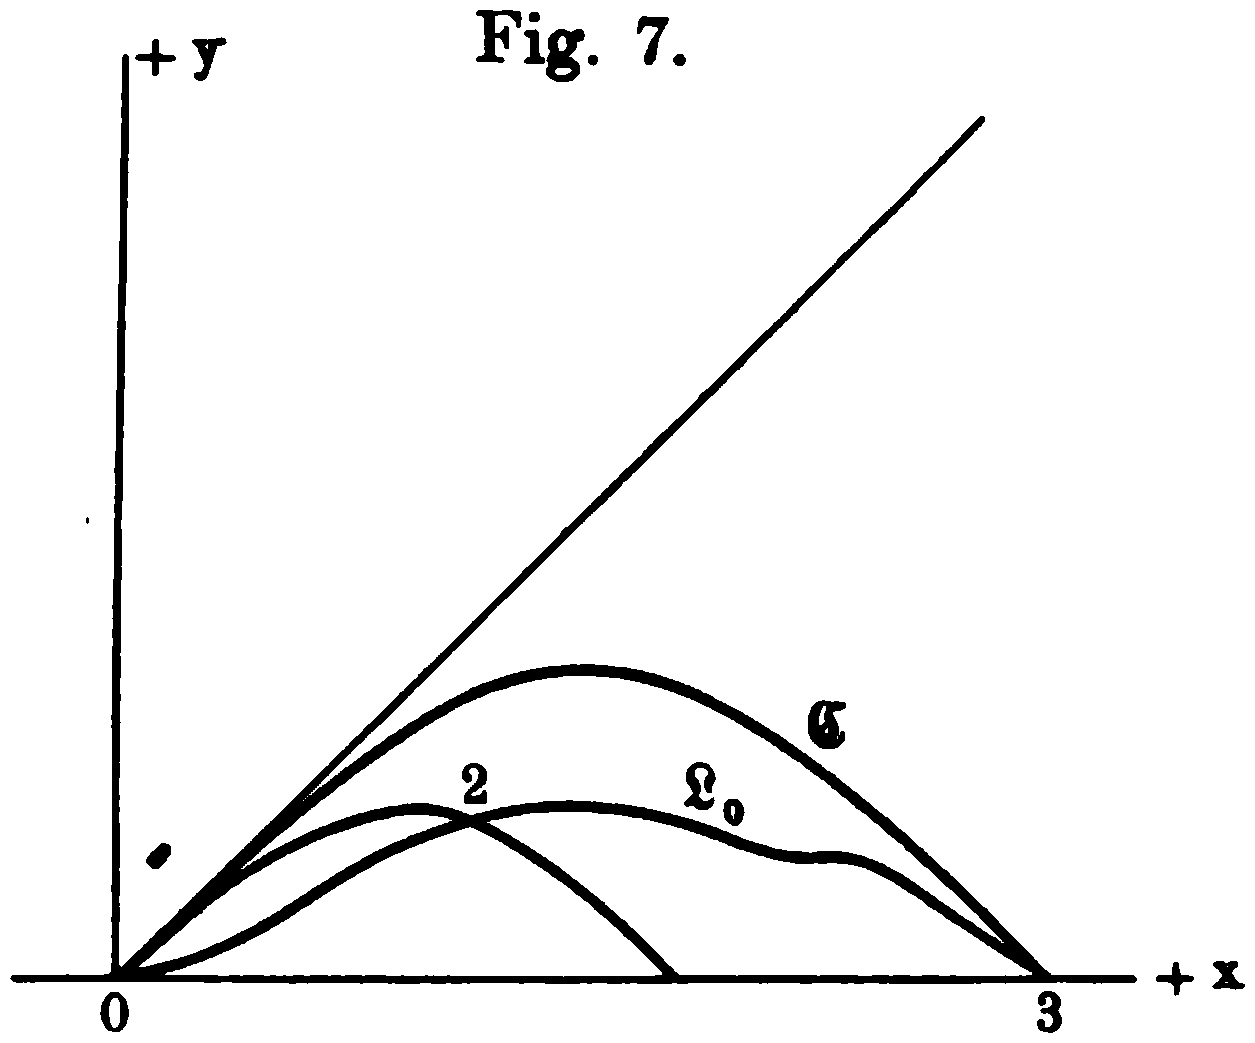
\includegraphics[width=\linewidth,height=32mm,keepaspectratio]{fig_assets/fig07_src_clean_x8.png}
\end{minipage}\hfill
\begin{minipage}[c]{0.49\linewidth}\centering
\end{minipage}
\end{center}

\[
f_{pp}\,dx=\frac{-y\,dx}{\left(\sqrt{1-p^2}\right)^3}
\]
negativ ist.

Derjenige Octant der $xy$-Ebene (Fig.~7), in welchem nach den letzten Ungleichungen (43) die Curve $\Omega_0$ liegt, wird nun von den Extremalen
\[
y=a\sin\frac{x}{a},\quad a>0,\quad p=\cos\frac{x}{a},
\]
auf deren jeder man
\begin{equation}\tag{44}
0\leqq\frac{x}{a}\leqq\pi
\end{equation}
annimmt, genau einfach bedeckt; denn hält man $x$ fest, so ist
\[
\frac{\partial y}{\partial a}
=\sin\frac{x}{a}-\frac{x}{a}\cos\frac{x}{a}
\]
% src-pdfpage=0087
% src-break=0087
wegen der für $x$ geltenden Ungleichung (44) stets positiv. Für $a=0$ hat man $y=0$, für $a=\infty$ dagegen $y=x$; der Punkt $(x,y)$ durchläuft also alle jenem Octanten angehörigen Punkte der Geraden $x=\text{const.}$ und jeden einmal, wenn $a$ alle positiven Werthe durchläuft. Man kann ferner $x=t$ setzen und hat dann
\[
\Delta=\frac{\partial(x,y)}{\partial(t,a)}
=\frac{\partial y}{\partial a},
\]
welche Grösse, wie bemerkt, positiv ist, so lange $y$ nicht verschwindet oder $=x$ wird. Entsprechen den Werthen $x=0$ und $x=a\pi$ die Punkte 0, 3, so ist jeder Theil des Extremalenbogens 03, der keinen der Endpunkte enthält, mit einem Felde umgeben; die Endpunkte selbst erfordern besondere Betrachtung, als in ihnen $p=\pm1$, die Function $F$ also singulär wird.

Setzen wir gemäss der allgemeinen Theorie im Falle, dass sich die Curve $\mathfrak{C}_0$ in den Punkt 0 zusammenzieht,
\[
u=\int_0^x y\sqrt{1-p^2}\,dx
=a\int_0^x\sin^2\frac{x}{a}\,dx
=\frac{ax}{2}-\frac{a^2}{2}\sin\frac{x}{a}\cos\frac{x}{a},
\]
wobei das positive Vorzeichen der Quadratwurzel benutzt ist, so verificirt man leicht mittelst der Ausdrücke
\[
F=y\sqrt{x'^2-y'^2},\quad
F_{x'}=\frac{yx'}{\sqrt{x'^2-y'^2}},\quad
F_{y'}=-\frac{yy'}{\sqrt{x'^2-y'^2}}
\]
die Gleichungen
\[
\frac{\partial u}{\partial a}
=
F_{x'}\frac{\partial x}{\partial a}
+
F_{y'}\frac{\partial y}{\partial a},
\quad
du=F_{x'}\,dx+F_{y'}\,dy.
\]
Dieses Differential $du$ kann nun auf keiner Curve $\Omega_0$ zwischen 0 und 3 verschwinden oder negativ werden; denn bezieht sich $d$ auf den Fortgang längs der Curve $\Omega_0$, dagegen $x',y',p$ auf die Extremale des Feldes, so würde sich, da $dx$ positiv ist, und für die Extremale $x=t$ gesetzt, also $F_{x'}$ als positiv angesehen werden kann, ergeben
\[
F_{x'}+F_{y'}\frac{dy}{dx}\leqq0,\quad
1+\frac{F_{y'}}{F_{x'}}\frac{dy}{dx}\leqq0,\quad
p\frac{dy}{dx}\geqq1,
\]
was nach der zweiten Ungleichung (43) und dem oben angegebenen Werthe von $p$ nur für $p=\pm1$, also in den Punkten der $x$-Axe eintreten kann. Die Grösse $du:d\tau$ ist daher zwischen
% src-pdfpage=0088
% src-break=0088
den Punkten 0 und 3 stets positiv, so dass man überall setzen kann
\[
dJ_{02}=du\left[1+\frac{s^2}{2}\,g_{ss}(u,v,\theta s)\right],
\]
woraus bei der oben erkannten Beschaffenheit des Ausdrucks $f_{pp}dx$ folgt
\[
\frac{d(J_{02}-u)}{d\tau}<0.
\]

Die Transformation des Differentials $dJ_{02}$ in die Variablen $u,v$ wird unmöglich, wenn
\[
dw=0,\quad dx=\pm dy,
\]
da dann der Integrand $F$ singulär ist. Trotzdem bleibt an solchen Stellen, wie die ursprüngliche Definition
\[
J=\int y\,\frac{dw}{d\tau}\,d\tau
\]
lehrt, $J_{02}$ eine Function $\varphi(\tau)$ im Sinne des \S~17. Dabei verschwindet offenbar $dJ_{02}:d\tau$, und für $du$ findet man
\[
du=dx(F_{x'}\pm F_{y'})=a\,dx\left(1\pm\cos\frac{x}{a}\right),
\]
so dass $d(u-J_{02})$ auch jetzt positiv bleibt. Die Grösse $u-J_{02}$ wächst also, wenn der Punkt 2 längs der Curve $\Omega_0$ von 0 nach 3 hin läuft.

Nähere Untersuchung erfordert wegen der Singularität des Punktes 0 der Anfangswerth von $u$. Derselbe ist zunächst offenbar Null, wenn die Ungleichung
\[
\left(\frac{dy}{d\tau}:\frac{dx}{d\tau}\right)^0<1
\]
besteht; dann bleibt nämlich die Grösse $a$, da sie nur für $x=y$ unendlich wird, bei der Annäherung an den Punkt 0 längs der Curve $\Omega_0$ unter einer endlichen Grenze; der Ausdruck für $u$ zeigt daher unmittelbar, dass $u$ mit $x$ gegen die Grenze Null convergirt. Hat man dagegen die Gleichungen
\[
\left(\frac{dy}{d\tau}:\frac{dx}{d\tau}\right)^0=1,\quad
\lim_{\tau=\tau_0}\frac{y}{x}=1,
\]
so lehrt die zur Definition von $a$ dienende Gleichung, d. h. wenn man setzt
\[
\varphi(z)=\frac{\sin z-z}{z},
\]
% src-pdfpage=0089
% src-break=0089
die Gleichung
\[
\frac{y}{x}=1+\varphi\left(\frac{x}{a}\right),
\]
dass man haben muss
\[
\left.\varphi\left(\frac{x}{a}\right)\right|^0=0.
\]
Nun ist die Grösse $\varphi(z)$ negativ, so lange $z$ zwischen 0 und $\pi$ liegt; hieraus folgt, da die Ungleichung (44) besteht, dass
\[
\varphi\left(\frac{x}{a}\right)
\]
nur dann verschwindet, wenn die Gleichung
\[
\frac{x}{a}=0
\]
besteht, welche somit für den Punkt 0 bewiesen ist. Dies gilt offenbar auch dann, wenn die Curve $\Omega_0$ ein endliches Stück mit der Geraden $y=x$ gemein hat und 0 den Punkt bedeutet, in welchem sich die Gerade und die Curve trennen. Substituirt man den erhaltenen Werth $\frac{x}{a}$ in die Gleichung
\[
u=\frac{a^2}{4}\left\{\frac{2x}{a}-\sin\frac{2x}{a}\right\}
=
\frac{1}{4}\left\{
\frac{(2x)^2}{3!}\cdot\frac{2x}{a}
-
\frac{(2x)^2}{5!}\left(\frac{2x}{a}\right)^3
+\cdots
\right\},
\]
so sieht man, dass auch in diesem Falle die Grösse $u$ als Function von $\tau$ mit dem Werthe 0 an der Stelle 0 beginnt. Da nun dasselbe von $J_{02}$ offenbar gilt, so hat man auch
\[
\left.u-J_{02}\right|_{\tau_0}=0,
\]
die Differenz $u-J_{02}$ ist also, da sie wächst, positiv, sobald der Punkt 2 den Bogen $\Omega_0$ entlang laufend die Gerade $y=x$ verlassen hat; ebenso ist auch der Grenzwerth
\[
\left.u\right|^3-J_{03}=\overline{J}_{03}-J_{03}
\]
positiv. Die Linien $\Omega$ und $\Omega^0$ umschliessen also mit der $w$-Axe eine kleinere Fläche als der Halbkreis von derselben Länge.

Der Satz, dass eine geschlossene Curve stets eine kleinere Fläche umschliesst, als ein Kreis von derselben Länge, folgt aus dem erhaltenen Resultate unmittelbar, wenn die Curve durch zwei ihrer Punkte 1 und 2 so in zwei gleich lange Stücke zerlegt werden kann, dass die gerade Strecke 12 ganz im Inneren verläuft; dieselbe kann dann mit der $w$-Axe identificirt werden.

\bigskip

\noindent\textbf{Aufgabe VI (\S~11).} Jedes Stück einer Extremale, welches den Rückkehrpunkt nicht enthält, kann man mit einem Felde
% src-pdfpage=0090
% src-break=0090
umgeben, indem man z. B. in den Gleichungen (17) die Grösse $a$ constant setzt und $b$ allein variiren lässt. Die Extremalen des Feldes sind dann Curven, die eine aus der anderen durch Verschiebung parallel der $x$-Axe hervorgehen; man hat daher, indem man $t=p$ setzt, die Gleichungen
\[
\frac{\partial x}{\partial b}=1,\quad
\frac{\partial y}{\partial b}=0,\quad
\Delta=-\frac{dy}{dp},
\]
und $\Delta$ kann nach (18) nur im Rückkehrpunkte verschwinden. Man findet ferner
\[
f_{pp}\,dx=-\frac{2yp(p^2-3)}{(1+p^2)^3}\,dx.
\]
Diese Grösse nimmt in Bogenelementen entgegengesetzter Richtung auch entgegengesetzte Werthe an, da der erste Fall des \S~3 vorliegt. Die \textsc{Legendre}'sche Vorzeichenbedingung für das starke Extremum ist also nicht erfüllt, wohl aber die für das schwache Extremum, da $p^2-3$ nur im Rückkehrpunkte das Zeichen wechselt. Ein Stück der Extremale, welches diesen nicht enthält, liefert daher ein schwaches Maximum oder Minimum, je nachdem es der einen oder anderen der Hälften angehört, in welche die Curve durch den Rückkehrpunkt zerlegt wird. Hat man $p^2<3$, so ist das gesuchte Minimum vorhanden.

\bigskip

\noindent\textbf{Aufgabe VII (\S~11).} Bei Einführung neuer Variablen $u,v$ hat man eine Transformation von der Form
\[
\sqrt{E\,d\varphi^2+2F\,d\varphi\,d\psi+G\,d\psi^2}
=
\sqrt{E^0\,du^2+2F^0\,du\,dv+G^0\,dv^2}
=
du\sqrt{E^0+2F^0s+G^0s^2};
\]
die Gleichungen
\[
g(u,v,0)=1,\quad g_s(u,v,0)=0
\]
ergeben daher
\[
E^0=1,\quad F^0=0.
\]
Dabei folgt aus dem Zusammenhange zwischen $E,E^0,F,\ldots$ und den Ableitungen der rechtwinkeligen Coordinaten nach $\varphi,\psi,u,v$ die Gleichung
\[
E^0G^0-F^0F^0=(EG-F^2)\left(\frac{\partial(\varphi,\psi)}{\partial(u,v)}\right)^2
\]
oder, wenn
\[
G^0=m^2
\]
gesetzt wird,
\[
\Delta=\frac{\partial(\varphi,\psi)}{\partial(u,v)}
=\frac{m}{\sqrt{EG-F^2}}.
\]
% src-pdfpage=0091
% src-break=0091

Die in \S~17 betrachtete besondere Form des Integranden ist also die \textsc{Gauss}'sche Form des Linienelementes
\[
\sqrt{du^2+m^2dv^2},
\]
und die zu einer gegebenen Linie senkrechten geodätischen Linien bilden in der Umgebung einer von ihnen ein Feld, so lange $m$ endlich und von Null verschieden ist.

Die \textsc{Legendre}'sche Bedingung des starken Minimums ist erfüllt, da in der Bezeichnung des \S~11
\[
\frac{\partial^2\Phi}{\partial\varphi'^2}
=
\frac{E}{\Phi}
-
\frac{(E\varphi'+F\psi')^2}{\Phi^3}
=
\frac{EG-F^2}{\Phi^3}\,\psi'^2,
\]
und diese Grösse stets positiv ist.

\begin{center}{\large \S~19.}\end{center}

Die rechten Seiten der für $u$ geltenden Gleichungen
\[
\frac{\partial u}{\partial x}=F_{x'},\quad
\frac{\partial u}{\partial y}=F_{y'}
\]
hängen nur von dem Verhältniss $y':x'$ ab; eliminirt man dasselbe, so ergiebt sich eine partielle Differentialgleichung erster Ordnung für $u$, die wir als die \textsc{Jacobi-Hamilton}'sche bezeichnen wollen. Ist $U$ irgend eine Lösung derselben, so kann man von den Gleichungen
\begin{equation}\tag{45}
\frac{\partial U}{\partial x}=F_{x'},\quad
\frac{\partial U}{\partial y}=F_{y'},
\end{equation}
die erste ansetzen und zur Bestimmung des Werthes $y':x'$ benutzen; die zweite ist dann von selbst erfüllt. Die erste Gleichung kann, indem man $U$ als gegeben ansieht, als gewöhnliche Differentialgleichung zwischen $x$ und $y$ aufgefasst werden, deren Integral
\begin{equation}\tag{46}
\varphi(x,y,a)=0
\end{equation}
sei und durch eine einfach unendliche Schar von Curven $\Omega$ dargestellt wird. Bezeichnet $D$ den Fortgang längs einer Curve $U=\text{const.}$, so hat man
\[
\frac{\partial U}{\partial x}Dx+\frac{\partial U}{\partial y}Dy=0,\quad
F_{x'}Dx+F_{y'}Dy=0;
\]
die Curven $\Omega$ liegen also transversal zu den Curven $U=\text{const.}$ Führt man ferner die Werthe einer beliebigen Function
\begin{equation}\tag{47}
t=\psi(x,y)
\end{equation}
% src-pdfpage=0092
% src-break=0092
längs einer bestimmten Curve $\Omega$ als Parameter ein, durch dessen Werthe $x$ und $y$ bestimmt sind, so ist
\[
x'=\frac{\partial x}{\partial t},\quad y'=\frac{\partial y}{\partial t},
\]
wobei man sich $x$ und $y$ aus den Gleichungen (46) und (47) als Functionen von $a$ und $t$ berechnet zu denken hat. Offenbar kann man auf Grund eben dieser Gleichungen auch $t$ und $a$ und damit $x'$ und $y'$ als Functionen von $x$ und $y$ betrachten; bezieht man das Zeichen $\partial$ auf diese Auffassung, während die Bezeichnung der Ableitungen durch Suffixe ihren bisherigen Sinn behält, so bestehen die Gleichungen
\begin{equation}\tag{48}
\frac{\partial F_{x'}}{\partial y}=\frac{\partial F_{y'}}{\partial x},
\end{equation}
\begin{equation}\tag{49}
\begin{aligned}
\frac{\partial F_{x'}}{\partial x}
&=
F_{x'x}+F_{x'x'}\frac{\partial x'}{\partial x}
+F_{x'y'}\frac{\partial y'}{\partial x},\\
\frac{\partial F_{y'}}{\partial x}
&=
F_{y'x}+F_{y'x'}\frac{\partial x'}{\partial x}
+F_{y'y'}\frac{\partial y'}{\partial x}.
\end{aligned}
\end{equation}
Weiter folgt, wie in \S~16 bemerkt ist, aus der Homogeneität der Functionen $F_{x'}$, $F_{y'}$
\begin{equation}\tag{50}
F_{x'x'}x'+F_{x'y'}y'=0,\quad
F_{y'x'}x'+F_{y'y'}y'=0,
\end{equation}
und hieraus auf Grund der Gleichungen (49), sowie der analogen, in denen nach $y$ differenzirt ist
\[
x'\frac{\partial F_{x'}}{\partial x}
+y'\frac{\partial F_{y'}}{\partial x}
=
x'F_{x'x}+y'F_{y'x}=F_x,
\]
\[
x'\frac{\partial F_{x'}}{\partial y}
+y'\frac{\partial F_{y'}}{\partial y}=F_y.
\]
Der Gleichung (48) zu Folge kann man aber den letzten Gleichungen auch folgende Form geben:
\[
F_x=
\frac{\partial F_{x'}}{\partial x}x'
+\frac{\partial F_{x'}}{\partial y}y'
=\frac{dF_{x'}}{dt},
\]
\[
F_y=
\frac{\partial F_{y'}}{\partial x}x'
+\frac{\partial F_{y'}}{\partial y}y'
=\frac{dF_{y'}}{dt},
\]
womit erhellt, dass die Curven $\Omega$ Extremalen des Integrals $J$ sind. Ist also $V$ irgend eine Lösung der durch Elimination von $x':y'$ aus den Gleichungen (45) entstehenden partiellen Differentialgleichung, so werden die Curven $V=\text{const.}$ von einer Schar von Extremalen des Integrals $J$ transversal geschnitten. Dabei ist offenbar, wenn man längs einer Curve $\Omega$ fortgeht,
% src-pdfpage=0093
% src-break=0093
\[
dV=(F_{x'}x'+F_{y'}y')\,dt=Fdt,
\]
man kann also setzen
\[
V=\int Fdt,
\]
wobei längs einer Extremale der Schar integriert ist.

Enthält die Function $V$ eine Constante $c$, so besagt die \textsc{Jacobi-Hamilton}'sche Gleichung, dass $p$ als Function von $x$ und $c$ so bestimmt werden kann, dass die Identitäten (45) bestehen. Differenziert man dieselben nach $c$, so erhält man
\[
\frac{\partial^2 V}{\partial x\,\partial c}
=
\frac{\partial F_{x'}}{\partial p}\frac{\partial p}{\partial c},\quad
\frac{\partial^2 V}{\partial y\,\partial c}
=
\frac{\partial F_{y'}}{\partial p}\frac{\partial p}{\partial c}.
\]
Nun kann man setzen
\[
F_{x'}=\psi\left(\frac{y'}{x'}\right)=\psi(p),
\]
also folgt
\[
F_{x'y'}=\frac{1}{x'}\psi'(p)=\frac{1}{x'}\frac{\partial F_{x'}}{\partial p}
\]
und Aehnliches gilt für $F_{y'}$; man erhält also
\[
\frac{\partial^2 V}{\partial x\,\partial c}
=
x'F_{x'y'}\frac{\partial p}{\partial c},\quad
\frac{\partial^2 V}{\partial y\,\partial c}
=
x'F_{y'y'}\frac{\partial p}{\partial c},
\]
und da die Gleichungen (50) gelten
\[
x'\frac{\partial^2V}{\partial x\,\partial c}
+
y'\frac{\partial^2V}{\partial y\,\partial c}=0.
\]
Längs jeder einzelnen Curve $\Omega$ besteht also eine Gleichung
\[
\frac{\partial V}{\partial c}=b;
\]
ist ihre linke Seite nicht constant, so stellt sie die Gesammtheit der Extremalen dar, so dass diese bekannt sind, wenn eine Function $V$ von den angegebenen Eigenschaften gefunden ist.

Die Verallgemeinerung dieser Theorie liegt nahe und möge für den Fall dreier Variablen angedeutet werden. Die Function $F(x,y,z,x',y',z')$ sei bezüglich der letzten drei Argumente homogen und von erster Dimension, so dass die Ableitungen $F_{x'}$, $F_{y'}$, $F_{z'}$ nur von $x,y,z$ und den Verhältnissen
\[
p=\frac{y'}{x'},\quad q=\frac{z'}{x'}
\]
abhängen. Gelten dann für eine Function $V$ die Gleichungen
\begin{equation}\tag{51}
\frac{\partial V}{\partial x}=F_{x'},\quad
\frac{\partial V}{\partial y}=F_{y'},\quad
\frac{\partial V}{\partial z}=F_{z'},
\end{equation}
% src-pdfpage=0094
% src-break=0094
sowie die hieraus durch Elimination von $p$ und $q$ folgende \textsc{Jacobi-Hamilton}'sche Differentialgleichung, so hat man, indem man die Differentiation $\partial$ ähnlich wie oben versteht,
\[
\frac{\partial F_{x'}}{\partial y}=\frac{\partial F_{y'}}{\partial x},\quad
\frac{\partial F_{y'}}{\partial z}=\frac{\partial F_{z'}}{\partial y},\quad
\frac{\partial F_{z'}}{\partial x}=\frac{\partial F_{x'}}{\partial z};
\]
hieraus folgt
\[
\frac{\partial F_{x'}}{\partial x}x'
+\frac{\partial F_{y'}}{\partial x}y'
+\frac{\partial F_{z'}}{\partial x}z'
=
\frac{\partial F_{x'}}{\partial x}x'
+\frac{\partial F_{x'}}{\partial y}y'
+\frac{\partial F_{x'}}{\partial z}z'
\]
nebst zwei analogen Gleichungen; dieselben ergeben, verbunden mit den Gleichungen, welche den unter (49) und (50) angeführten entsprechen,
\[
F_x-\frac{dF_{x'}}{dt}=0,\quad
F_y-\frac{dF_{y'}}{dt}=0,\quad
F_z-\frac{dF_{z'}}{dt}=0.
\]
Fasst man daher zwei der Gleichungen (51) als gewöhnliche Differentialgleichungen zwischen $x,y,z$ auf, so sind die ihre Integrale darstellenden Curven Extremalen des Integrals $\int Fdt$. Enthält ferner $V$ zwei Constante $c_1,c_2$, so ergeben die Gleichungen (51)
\[
\frac{\partial^2V}{\partial x\,\partial c_1}
=
\frac{\partial F_{x'}}{\partial p}\frac{\partial p}{\partial c_1}
+
\frac{\partial F_{x'}}{\partial q}\frac{\partial q}{\partial c_1}
=
x'\left(
F_{y'x'}\frac{\partial p}{\partial c_1}
+
F_{z'x'}\frac{\partial q}{\partial c_1}
\right)
\]
nebst zwei ähnlichen Gleichungen, aus welchen sich nach den analogen der Gleichungen (50) ergibt
\[
x'\frac{\partial^2V}{\partial x\,\partial c_\alpha}
+
y'\frac{\partial^2V}{\partial y\,\partial c_\alpha}
+
z'\frac{\partial^2V}{\partial z\,\partial c_\alpha}
=0,\quad \alpha=1,2.
\]
Die Gleichungen
\[
\frac{\partial V}{\partial c_1}=b_1,\quad
\frac{\partial V}{\partial c_2}=b_2
\]
stellen also die Extremalen des Integrals $\int Fdt$ dar. Enthält dasselbe $n+1$ Grössen $x,y,z,\ldots$, so muss $V$ mit $n$ willkürlichen Constanten behaftet sein, damit es zur Darstellung aller Extremalen dienen könne.

\bigskip

\noindent\textbf{Beispiel.} Ist $x$ die Zeit, $y,z,\ldots$ die unabhängigen Parameter eines Massensystems, und setzt man
\[
p=\frac{dy}{dx},\quad q=\frac{dz}{dx},\ldots,
\]
so ist das \textsc{Hamilton}'sche Princip meistens eine Gleichung von der Form
% src-pdfpage=0095
% src-break=0095
\[
\delta\int H(x,y,z,\ldots,p,q,\ldots)\,dx=0,
\]
wobei zwischen zwei gegebenen Werthsystemen $(x,y,z,\ldots)$ zu integrieren ist; $H$ heisst nach \textsc{Helmholtz} das kinetische Potential. Will man das Integral auf die Form
\[
\int Fdt
\]
bringen, so hat man zu setzen
\[
p=\frac{y'}{x'},\quad q=\frac{z'}{x'},\ldots,\quad
F=x'H(x,\ldots,p,q,\ldots),
\]
so dass
\[
F_{x'}=H-p\frac{\partial H}{\partial p}-q\frac{\partial H}{\partial q}-\cdots,\quad
F_{y'}=\frac{\partial H}{\partial p},\quad
F_{z'}=\frac{\partial H}{\partial q},\ldots
\]
Die \textsc{Jacobi-Hamilton}'sche Gleichung entsteht daher durch Elimination von $p,q,\ldots,$ aus den Gleichungen
\begin{equation}\tag{52}
\frac{\partial V}{\partial x}
=
H-p\frac{\partial H}{\partial p}
-q\frac{\partial H}{\partial q}-\cdots,\quad
\frac{\partial V}{\partial y}
=
\frac{\partial H}{\partial p},\ldots
\end{equation}
Kommt die Zeit $x$ in $H$ nicht explicit vor, so besteht für die Extremalen die Gleichung
\begin{equation}\tag{53}
F_{x'}=\text{const.},\quad
p\frac{\partial H}{\partial p}
+
q\frac{\partial H}{\partial q}
+\cdots-H=-h,
\end{equation}
und $h$ ist die verallgemeinerte Constante der lebendigen Kraft. Da sich nun auch in den Gleichungen (52) die Grössen $p,q,\ldots,$ auf die Extremalen beziehen, so hat man
\[
\frac{\partial V}{\partial x}=h,\quad V=hx+W,
\]
wobei $W$ die Zeit nicht explicit enthält, und den Gleichungen
\[
\frac{\partial W}{\partial y}
=
\frac{\partial H}{\partial p},\quad
\frac{\partial W}{\partial z}
=
\frac{\partial H}{\partial q},\ldots
\]
genügt. Ist $n+1$ die Anzahl der Grössen $x,y,\ldots$, so dass das System $n$ Grade der Bewegungsfreiheit hat, und sind $n-1$ Constante $c_1,c_2,\ldots,c_{n-1}$ in $W$ enthalten, so werden die Bewegungen des Systemes durch die folgenden Gleichungen dargestellt:
\[
\frac{\partial V}{\partial c_1}=\frac{\partial W}{\partial c_1}=b_1,\quad
\frac{\partial V}{\partial c_2}=\frac{\partial W}{\partial c_2}=b_2,\ldots,\quad
\frac{\partial V}{\partial h}=x+\frac{\partial W}{\partial h}=x_0,
\]
in welchen rechts willkürliche Constanten stehen.

Diese Betrachtung ist von der Form der Function $H$ unabhängig. Hat man speciell
% src-pdfpage=0096
% src-break=0096
\[
-H=T+U
\]
und ist $T$ eine quadratische Form der Grössen $p,q,\ldots$, $U$ aber von diesen frei, so geht die Gleichung (53), da jetzt
\[
2T=p\frac{\partial T}{\partial p}+q\frac{\partial T}{\partial q}+\cdots,
\]
in die gewöhnliche Gleichung der lebendigen Kraft über:
\[
T=U+h.
\]


% src-pdfpage=0096
% src-break=0096
% unit: sec20_open source=kneser_lvr_1900_archiveorg.pdf#p0096 portion=lower authorial=true
\begin{center}{\large \S~20.}\end{center}

Wie in \S~14, dessen Voraussetzungen jetzt allein festgehalten werden sollen, sei $\mathfrak{C}_0$ eine beliebige reguläre Curve (Fig.~8), welche, von $\mathfrak{C}$ ausgehend, den Extremalen des Feldes unter einem nicht verschwindenden Winkel begegnet und vom Punkte 0 durchlaufen wird; 12 sei irgend ein den Punkt 0 nicht enthaltendes Stück der Curve $\mathfrak{C}$.

% unit: fig8 source=kneser_lvr_1900_archiveorg.pdf#p0096 authorial=true type=hq_sourcecrop


\begin{center}
{\small Fig.~8.}\par\vspace{1mm}
\begin{minipage}[c]{0.47\linewidth}\centering
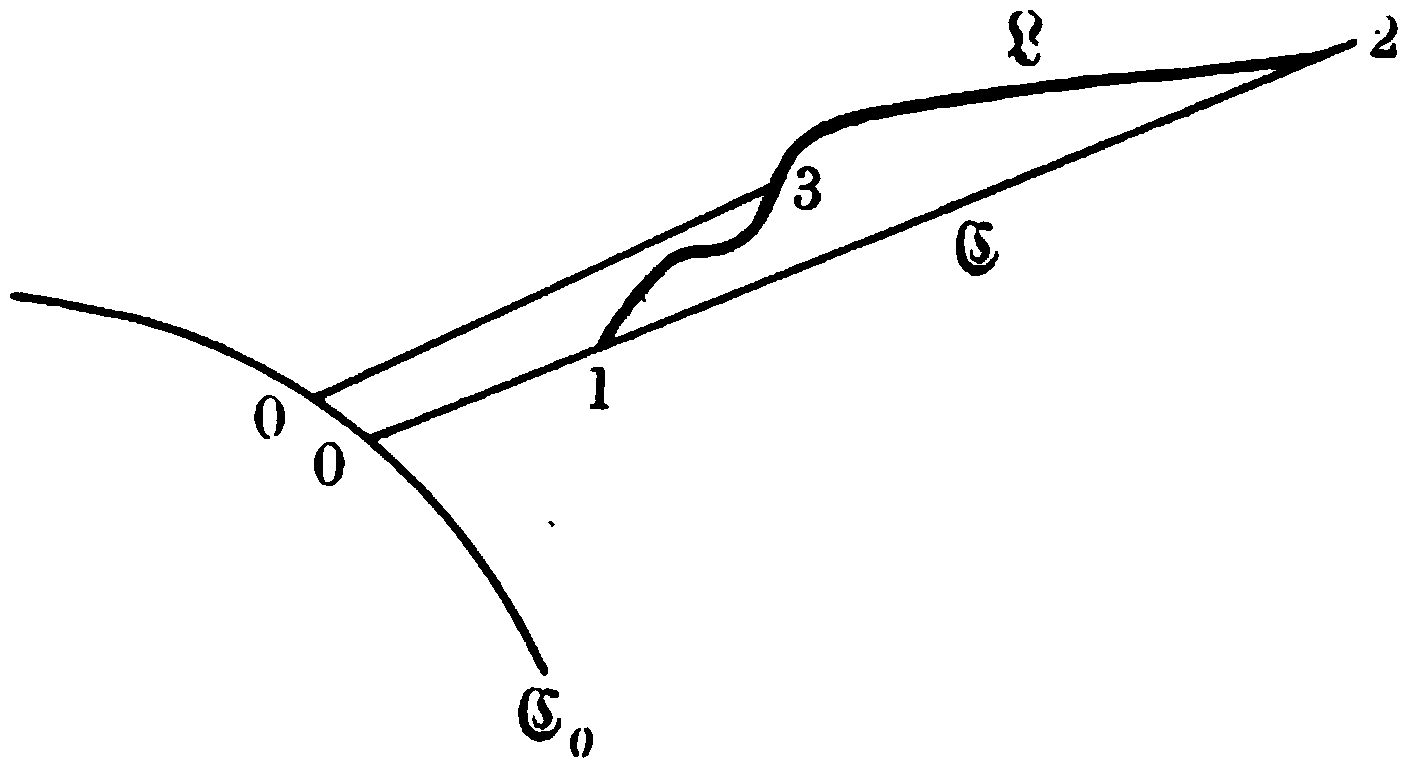
\includegraphics[width=\linewidth,height=32mm,keepaspectratio]{fig_assets/fig08_src_clean_x8.png}
\end{minipage}\hfill
\begin{minipage}[c]{0.49\linewidth}\centering
\end{minipage}
\end{center}

 Die Punkte 1 und 2 seien durch eine weitere dem Felde angehörige Curve $\Omega$ verbunden, längs deren der Punkt 3 von 1 nach 2 laufe. Diese Curve habe die Eigenschaften der in \S~17 ebenso bezeichneten, so dass $x_3,y_3$ Functionen eines Parameters $\tau$ sind, welche zu den dort untersuchten $\varphi(\tau)$ gehören; der Parameter $t$ wachse in der Richtung von 1 nach 2 hin. Durch jede Lage des Punktes 3 geht dann eine bestimmte Extremale des Feldes, deren Parameter $a$ ebenso wie das auf ihr dem Punkte 3 entsprechende Argument $t$ nach \S~14 reguläre Functionen von $x_3,y_3$ sind. Diese Extremale schneidet auf der Curve $\mathfrak{C}_0$ einen Punkt 0 aus, dessen Coordinaten ebenso wie das ihr zugehörige Argument $t_0$ nach \S~14 reguläre Functionen von $a$ und bei hinreichender Beschränkung des Feldes, sowie des Curvenstückes $\mathfrak{C}_0$ eindeutig bestimmt sind. Setzt man daher
\[
\omega(a)=
F(\xi,\eta,\xi_t,\eta_t)\frac{dt_0}{da}
+F_{x'}(\xi,\ldots,\eta_t)\xi_a
+F_{y'}(\xi,\ldots,\eta_t)\eta_a\bigg|^0,
\]
so ist dieser Ausdruck eine reguläre Function von $a$; wenn wiederum
\[
u=\overline{J}_{03}
\]
% src-pdfpage=0097
% src-break=0097
gesetzt wird, lehrt die Formel (31)
\[
\frac{\partial u}{\partial a}
=
\frac{\partial\overline{J}_{03}}{\partial a}
=
-\omega(a)+F_{x'}(\xi,\ldots,\eta_t)\xi_a
+F_{y'}(\xi,\ldots,\eta_t)\eta_a\bigg|^3,
\]
und wenn der Punkt 3 auf einer bestimmten Extremale 03 beweglich gedacht wird, ergiebt sich unmittelbar
\[
\frac{\partial u}{\partial t}=F(\xi,\eta,\xi_t,\eta_t)\bigg|^3.
\]
Nun sind $a,t$ ebenso wie $x_3,y_3$ Functionen von $\tau$, welche zu den in \S~17 durch $\varphi(\tau)$ bezeichneten gehören; bezieht sich daher jede Differentiation nach $\tau$ stets auf vordere Ableitungen, so ergeben die letzten beiden Gleichungen
\[
\frac{d\overline{J}_{03}}{d\tau}
=
-\omega(a)\frac{da}{d\tau}
+F_{x'}(\xi,\ldots,\eta_t)\frac{dx}{d\tau}
+F_{y'}(\xi,\ldots,\eta_t)\frac{dy}{d\tau}\bigg|^3.
\]
Ferner genügt das längs der Curve $\Omega$ gebildete Integral $J_{32}$, welches als Function von $\tau$ ebenfalls den Charakter von $\varphi(\tau)$ hat, der Gleichung
\[
\frac{dJ_{32}}{d\tau}
=
-F\left(x,y,\frac{dx}{d\tau},\frac{dy}{d\tau}\right)\bigg|^3;
\]
man erhält daher, indem man $\xi_t,\eta_t$ durch $x',y'$ ersetzt,
\[
\frac{d(\overline{J}_{03}+J_{32})}{d\tau}
=
-\omega(a)\frac{da}{d\tau}
+F_{x'}(x,y,x',y')\frac{dx}{d\tau}
\]
\[
\qquad
+F_{y'}(x,y,x',y')\frac{dy}{d\tau}
-F\left(x,y,\frac{dx}{d\tau},\frac{dy}{d\tau}\right).
\]
Die Summe der letzten drei Glieder heisse $\mathfrak{E}$ oder genauer
\[
\mathfrak{E}\left(x,y,x',y',\frac{dx}{d\tau},\frac{dy}{d\tau}\right).
\]
Liegt nun der Punkt 3 speciell in seiner Anfangslage 1 und seiner Endlage 2, so sind die entsprechenden Werthe der Summe $\overline{J}_{03}+J_{32}$
\[
\overline{J}_{01}+J_{12},\quad
\overline{J}_{02}=\overline{J}_{01}+\overline{J}_{12},
\]
somit folgt für die Differenz beider
\[
\overline{J}_{12}-J_{12}
=
\int_{\tau_1}^{\tau_2}
\frac{d(\overline{J}_{03}+J_{32})}{d\tau}\,d\tau
=
-\int_{\tau_1}^{\tau_2}\omega(a)\frac{da}{d\tau}\,d\tau
+\int_{\tau_1}^{\tau_2}\mathfrak{E}\,d\tau.
\]
Der erste Summand rechts verschwindet aber; denn setzt man
\[
\int \omega(a)\,da=\xi(a),
\]
% src-pdfpage=0098
% src-break=0098
so ist $\xi$ ebenfalls eine für $a=a_0$ reguläre Function, und man hat
\[
\int_{\tau_1}^{\tau_2}\omega(a)\frac{da}{d\tau}\,d\tau
=
\int_{\tau_1}^{\tau_2}\frac{d\xi(a)}{d\tau}\,d\tau
=
\xi(a)\bigg|_1^2;
\]
diese Grösse hat aber den Werth 0, da $a$ in den Punkten 1 und 2 denselben Werth $a_0$ hat. Somit folgt
\begin{equation}\tag{54}
\overline{J}_{12}-J_{12}
=
-\int_{\tau_1}^{\tau_2}
\mathfrak{E}\left(x,y,x',y',\frac{dx}{d\tau},\frac{dy}{d\tau}\right)d\tau,
\end{equation}
und die linke Seite hat ein festes Vorzeichen, wenn dasselbe von $\mathfrak{E}$ gilt.

Will man in dem Falle, dass alle Extremalen des Feldes im Punkte 0 zusammenlaufen, gerade den Extremalenbogen 02 prüfen, so ersetzt man nur die Curve $\mathfrak{C}_0$ durch den festen Punkt 0; die Formel
\begin{equation}\tag{55}
d\overline{J}_{03}=du=F_{x'}\,dx+F_{y'}\,dy,
\end{equation}
die wir nöthigenfalls durch specielle Betrachtungen bewiesen haben müssen, ergiebt sofort
\begin{equation}\tag{56}
\frac{d(\overline{J}_{03}+J_{32})}{d\tau}=\mathfrak{E},\quad
J_{02}-\overline{J}_{02}
=
-\int_{\tau_0}^{\tau_2}\mathfrak{E}\,d\tau,
\end{equation}
so lange nur die zum Vergleich herangezogene Curve $\Omega$ innerhalb der Fläche bleibt, welche die vom Punkte 0 ausgehenden Extremalen einfach bedecken.

Die einfache Formel (55) für $du$ bleibt nach \S~15 auch dann gültig, wenn die Curve $\mathfrak{C}_0$ von den Extremalen des Feldes transversal geschnitten wird (Fig.~9); dann verschwindet $\omega(a)$ identisch.

% unit: fig9 source=kneser_lvr_1900_archiveorg.pdf#p0098 authorial=true type=hq_sourcecrop


\begin{center}
{\small Fig.~9.}\par\vspace{1mm}
\begin{minipage}[c]{0.47\linewidth}\centering
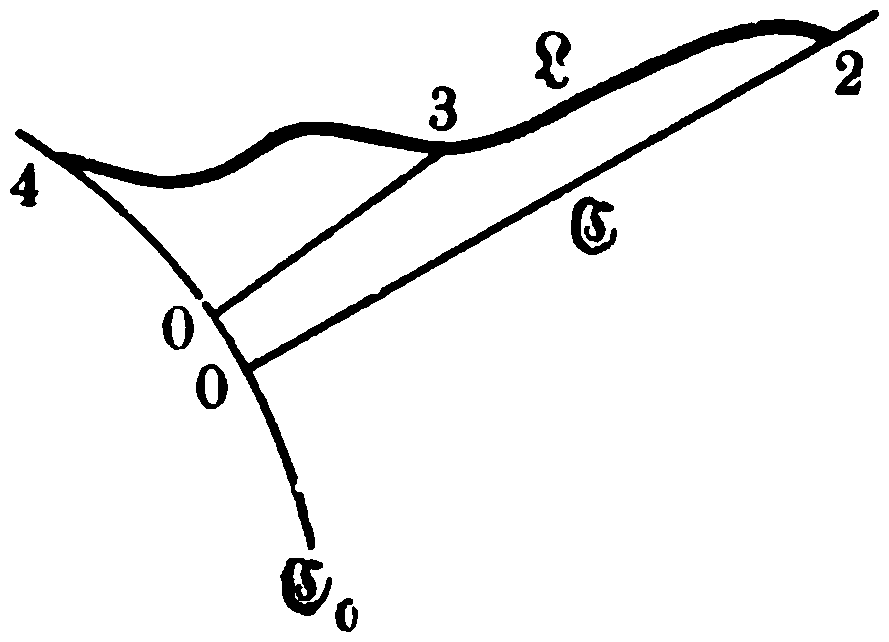
\includegraphics[width=\linewidth,height=32mm,keepaspectratio]{fig_assets/fig09_src_clean_x8.png}
\end{minipage}\hfill
\begin{minipage}[c]{0.49\linewidth}\centering
\end{minipage}
\end{center}

 Hiervon machen wir Gebrauch, um mittelst des Ausdruckes $\mathfrak{E}$ auch für das Extremum mit einer variablen Grenze ein Kriterium herzuleiten. Der Punkt 4 liege auf der Curve $\mathfrak{C}_0$, 2 wie bisher auf der Curve $\mathfrak{C}$; beide seien durch eine im Felde verbleibende Curve $\Omega$ verbunden, welche vom Punkte 3 in der Richtung von 4 nach 2 hin durchlaufen wird. Dann sind Anfangs- und Endwerth der Summe $\overline{J}_{03}+J_{32}$ die Grössen
\[
J_{42},\quad \overline{J}_{02},
\]
% src-pdfpage=0099
% src-break=0099
und man hat wie bisher
\[
\frac{d\overline{J}_{03}}{d\tau}
=
F_{x'}\frac{dx}{d\tau}
+F_{y'}\frac{dy}{d\tau},
\quad
\frac{dJ_{32}}{d\tau}
=
-F\left(x,y,\frac{dx}{d\tau},\frac{dy}{d\tau}\right),
\]
also
\begin{equation}\tag{57}
J_{42}-\overline{J}_{02}
=
-\int_{\tau_4}^{\tau_2}\mathfrak{E}\,d\tau.
\end{equation}





\begin{center}{\large \S~21.}\end{center}

Die Grösse $\mathfrak{E}$, durch deren Untersuchung hiernach die Frage nach dem Eintreten des Extremums entschieden werden kann, hängt offenbar von dem Punkte 2 $(x,y)$ und den beiden von ihm ausgehenden Linienelementen ab, welche auf der Extremale des Feldes und der Curve $\Omega$ durch den Sinn wachsender Parameter $t$ und $\tau$ bestimmt werden. Sind beide Grössen $x'$ und $\dfrac{dx}{d\tau}$ von Null verschieden, so dass man setzen kann
\[
D x=\frac{dx}{d\tau}\,d\tau,\quad
D y=\frac{dy}{d\tau}\,d\tau=\bar{p}\,D x,\quad
dy=p\,dx,
\]
\[
F(x,y,x',y')dt=f(x,y,p)dx,
\]
\[
F\left(x,y,\frac{dx}{d\tau},\frac{dy}{d\tau}\right)d\tau
=
f(x,y,\bar{p})D x,
\]
so ergiebt sich
\begin{equation}\tag{58}
\mathfrak{E}\,d\tau
=
\{f(x,y,p)+(\bar{p}-p)f_p(x,y,p)-f(x,y,\bar{p})\}D x.
\end{equation}
Zwar kommen die das erstere Linienelement charakterisirenden Grössen $x'$ und $y'$ nur in $F_{x'}$ und $F_{y'}$ vor, welche Ausdrücke nur von $x':y'$ abhängen. Daraus kann aber nicht geschlossen werden, dass $\mathfrak{E}$ denselben Werth behält, wenn man das Element der Extremale durch sein entgegengesetztes ersetzt; denn wenn auch $F$ eine eindeutige Function von $x'$ und $y'$ ist, so brauchen (\S~3) doch $F_{x'}$ und $F_{y'}$ nicht eindeutige Functionen von $x':y'$ zu sein. Die Grössen
\[
\mathfrak{E}\left(x,y,x',y',\frac{dx}{d\tau},\frac{dy}{d\tau}\right),\quad
\mathfrak{E}\left(x,y,-x',-y',\frac{dx}{d\tau},\frac{dy}{d\tau}\right)
\]
brauchen also nicht gleich, ebenso wenig die Grössen
\[
\mathfrak{E}\left(x,y,x',y',\frac{dx}{d\tau},\frac{dy}{d\tau}\right),\quad
\mathfrak{E}\left(x,y,x',y',-\frac{dx}{d\tau},-\frac{dy}{d\tau}\right)
\]
entgegengesetzt zu sein (Beispiele unten).

% src-pdfpage=0100
% src-break=0100
Die beiden Linienelemente, von denen $\mathfrak{E}$ abhängt, fallen dann und nur dann zusammen, wenn eine positive Grösse $\alpha$ existirt, welche den Gleichungen
\begin{equation}\tag{59}
x'=\alpha\frac{dx}{d\tau},\quad
y'=\alpha\frac{dy}{d\tau}
\end{equation}
genügt. In diesem Falle hat man
\[
F_{x'}(x,y,x',y')
=
F_{x'}\left(x,y,\frac{dx}{d\tau},\frac{dy}{d\tau}\right),
\]
\[
F_{y'}(x,y,x',y')
=
F_{y'}\left(x,y,\frac{dx}{d\tau},\frac{dy}{d\tau}\right);
\]
da nun immer
\[
\frac{dx}{d\tau}F_{x'}\left(x,y,\frac{dx}{d\tau},\frac{dy}{d\tau}\right)
\]
\[
+
\frac{dy}{d\tau}F_{y'}\left(x,y,\frac{dx}{d\tau},\frac{dy}{d\tau}\right)
-
F\left(x,y,\frac{dx}{d\tau},\frac{dy}{d\tau}\right)=0,
\]
so folgt
\[
\mathfrak{E}=0.
\]
Wir sagen dann, $\mathfrak{E}$ verschwinde in ordentlicher Weise. Nimmt $\mathfrak{E}$ den Werth Null an, ohne dass die Gleichungen (59) mit einem positiven Werthe $\alpha$ bestehen, so nennen wir das Verschwinden ausserordentlich.

Geometrisch kann die Bedeutung der Grösse $\mathfrak{E}$ gekennzeichnet werden, wenn wir vorausnehmen, was wir später (\S~30) beweisen, sonst aber jetzt nicht gebrauchen, dass jedes hinreichend kleine Stück einer Extremale im Allgemeinen mit einem Felde umgeben werden kann. Es seien 78 und 79 die Linienelemente (Fig.~10), welche zu den Werthsystemen $(x,y,dx,dy)$, $(x,y,Dx,Dy)$ gehören;

% unit: fig10 source=kneser_lvr_1900_archiveorg.pdf#p0100 authorial=true type=hq_sourcecrop


\begin{center}
{\small Fig.~10.}\par\vspace{1mm}
\begin{minipage}[c]{0.47\linewidth}\centering
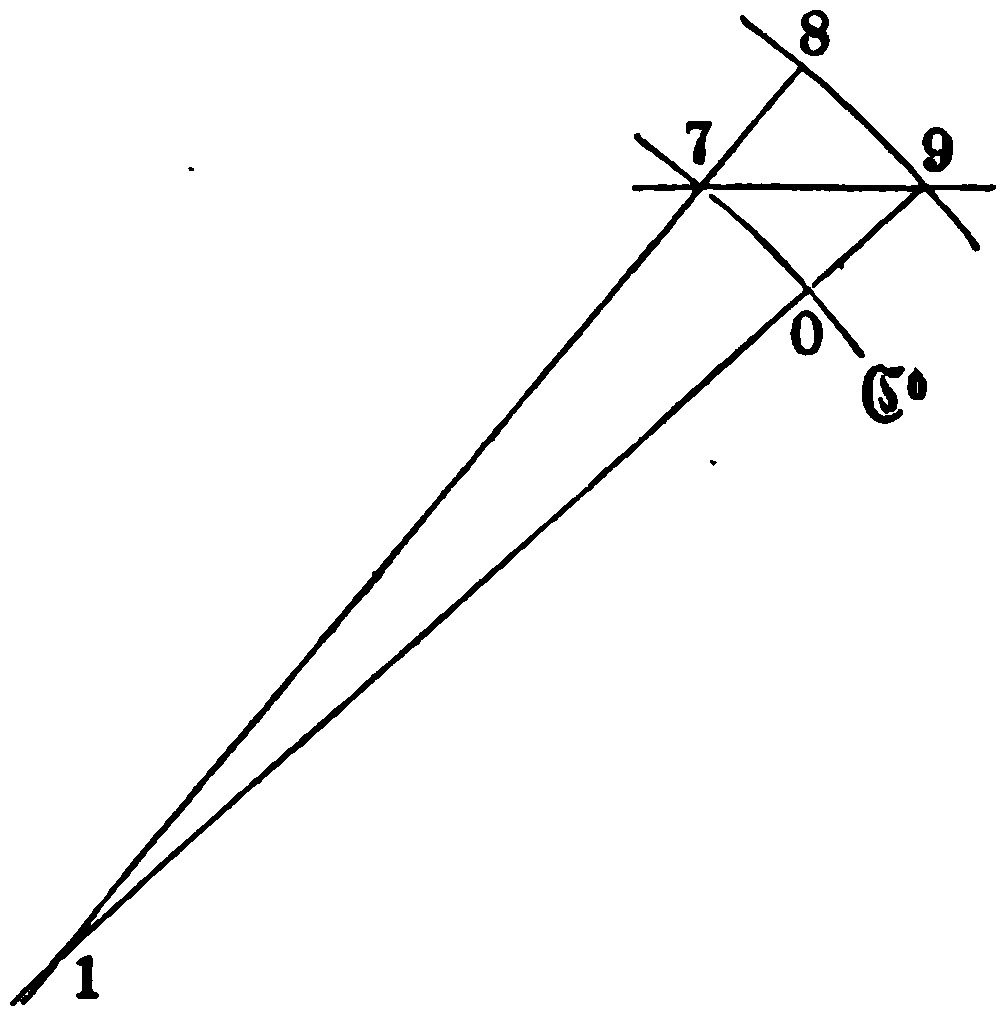
\includegraphics[width=\linewidth,height=32mm,keepaspectratio]{fig_assets/fig10_src_clean_x8.png}
\end{minipage}\hfill
\begin{minipage}[c]{0.49\linewidth}\centering
\end{minipage}
\end{center}

 dann ziehe man in der Richtung 78 eine Extremale, und umgebe sie in der Nähe des Punktes 7 mit einem Felde, dessen Extremalen die durch den Punkt 7 gehende Curve $\mathfrak{C}^0$, sowie eine Curve 89 transversal schneiden mögen. Erstere werde im Punkte 0 von der durch 9 gehenden Extremale des Feldes geschnitten; dann kann $\overline{J}_{09}$ oder $\overline{J}_{78}$ als Differential der von der Curve $\mathfrak{C}^0$ ab gerechneten Grösse $u$ im Sinne des
% src-pdfpage=0101
% src-break=0101
\S~15 angesehen werden und man hat nach der Formel (34)
\[
\overline{J}_{09}=\overline{J}_{78}
=
F_{x'}(x,y,dx,dy)D x+F_{y'}(x,y,dx,dy)D y.
\]
Schneiden sich die Extremalen 78 und 09 in einem Punkte 1, der von 7 aus nach der entgegengesetzten Seite wie 8 liegt, so ist nach \S~15
\[
\overline{J}_{17}=\overline{J}_{10},\quad
\mathfrak{E}\,d\tau
=
\overline{J}_{78}-J_{79}
=
\overline{J}_{19}-\overline{J}_{17}-J_{79}.
\]
Man sieht hieraus, dass die Grösse $\mathfrak{E}d\tau$ vom Coordinatensystem unabhängig ist, was auch durch die in \S~16 entwickelte Identität
\[
F_{x'}(x,y,dx,dy)D x+F_{y'}(x,y,dx,dy)D y
\]
\[
=
G_{u'}(u,v,du,dv)D u+G_{v'}(u,v,du,dv)D v
\]
ersichtlich wird.

Speciell kann man daher das Coordinatensystem so gedreht denken, dass für die zwei Elemente 78 und 79 das Differential $dx$ dasselbe Vorzeichen hat, d. h. dass beide Elemente nach derselben Seite einer Parallele zur $y$-Axe hinweisen. Dann sind
\[
p=\frac{dy}{dx},\quad
\bar{p}=\frac{dy}{d\tau}:\frac{dx}{d\tau}=D y:D x
\]
endliche Grössen, und die Elemente definirt durch die Werthsysteme $(x,y,p,dx)$, $(x,y,\bar{p},dx)$. Ist nun $F$ für alle vom Punkte $(x,y)$ ausgehenden Bogenelemente regulär, so gilt nach \S~5 dasselbe von
\[
f(x,y,p)=\frac{F}{x'}
\]
für alle Elemente, welche in den von den Richtungen 78 und 79 gebildeten concaven Winkel fallen, da für sie $x'$ von Null verschieden ist; $f$ ist also für das Intervall von $p$ bis $\bar{p}$ regulär, und man kann, wenn $\theta$ ein echter Bruch ist, nach (58) setzen
\[
f(x,y,\bar{p})=f(x,y,p)+(\bar{p}-p)f_p(x,y,p)
+\frac{1}{2}(\bar{p}-p)^2 f_{pp}[x,y,p+\theta(\bar{p}-p)],
\]
\begin{equation}\tag{60}
\mathfrak{E}d\tau
=
-\frac{1}{2}(\bar{p}-p)^2 f_{pp}[x,y,p+\theta(\bar{p}-p)]\,dx.
\end{equation}
Die Grösse $\mathfrak{E}$ hat das feste Vorzeichen von $-F_1$ und verschwindet nur in ordentlicher Weise, wenn die \textsc{Legendre}'sche Bedingung des starken Extremums erfüllt ist; denn das Product
\[
f_{pp}[x,y,p+\theta(\bar{p}-p)]\,dx
\]
ist identisch mit der Grösse $F_1(x,y,dx,dy)dx^4$, welche zu dem durch den Punkt $(x,y)$ gehenden Bogenelemente gehört, dessen Componenten
\[
dx,\ [p+\theta(\bar{p}-p)]dx=dy
\]
% src-pdfpage=0102
% src-break=0102
sind, womit die ausgesprochene Behauptung bewiesen ist. Wenn jedoch nur die \textsc{Legendre}'sche Bedingung des schwachen Extremums als erfüllt vorausgesetzt wird, hat $\mathfrak{E}$ die bezeichneten beiden Eigenschaften nur, so lange die beiden bestimmenden Elemente 78, 79 von einem in der Integrationsrichtung genommenen Element der Curve $\mathfrak{C}$ nach Lage und Richtung hinreichend wenig abweichen. Umgekehrt wird man nicht in gleicher Weise vom Zeichen der Grösse $\mathfrak{E}$ auf das der Grösse $F_1$ schliessen können.



\begin{center}{\large \S~22.}\end{center}

Allgemein hat man, wenn $t$ und $a$ sich auf den Punkt 3 beziehen, der die Curve $\Omega$ durchläuft,
\[
x=\xi(t,a),\quad y=\eta(t,a),
\]
\[
\frac{dx}{d\tau}=\xi_t\frac{dt}{d\tau}+\xi_a\frac{da}{d\tau},\quad
\frac{dy}{d\tau}=\eta_t\frac{dt}{d\tau}+\eta_a\frac{da}{d\tau},
\]
\[
x'=\xi_t,\quad y'=\eta_t.
\]
Wenn nun längs der ganzen Curve $\Omega$ die Grösse $\mathfrak{E}$ in allen Punkten ordentlich verschwände, so würden sich die Gleichungen (59) ergeben, und damit
\[
\begin{vmatrix}
x' & \dfrac{dx}{d\tau}\\[0.7em]
y' & \dfrac{dy}{d\tau}
\end{vmatrix}
=
\begin{vmatrix}
\xi_t & \xi_a\dfrac{da}{d\tau}\\[0.7em]
\eta_t & \eta_a\dfrac{da}{d\tau}
\end{vmatrix}
=
\Delta\frac{da}{d\tau}=0.
\]
Da nun $\Delta$ von Null verschieden ist, so folgt für ein endliches Intervall des Arguments $\tau$:
\[
\frac{da}{d\tau}=0.
\]
Hieraus folgt, da $a$ als Function von $\tau$ die Eigenschaften der in \S~17 definirten Function $\varphi(\tau)$ hat, dass $a$ längs der ganzen Curve $\Omega$ constant und seinem Anfangswerth $a_0$ gleich sein muss.

Fällt also die Curve $\Omega$ mit $\mathfrak{C}$ nicht vollkommen zusammen, ist ferner ein ausserordentliches Verschwinden der Grösse $\mathfrak{E}$ entweder überhaupt oder durch Beschränkungen der Curven $\Omega$ ausgeschlossen, und findet beim ordentlichen Verschwinden längs der Curve $\Omega$ kein Zeichenwechsel statt, so sind die rechten Seiten der Gleichungen (54), (56), (57) in \S~20 von Null verschieden und
% src-pdfpage=0103
% src-break=0103
festen Vorzeichens. Die Extremalen 12, 02 ergeben also gegenüber den in der angegebenen Weise beschränkten Curven $\Omega$ in der That ein Extremum des Integrals $J$, und zwar ein Maximum oder Minimum, je nachdem $\mathfrak{E}$ positiv oder negativ ist.

Liegt speciell die Curve $\Omega$ in einer engeren, durch $\rho$ und $\rho_1$ nach \S~17 definirten Nachbarschaft des Bogens 12 der Curve $\mathfrak{C}$, so liegt der Winkel einer im Sinne wachsender $t$ gezogenen Tangente des letzteren mit einer ebensolchen Tangente einer Extremale des Feldes, deren Berührungspunkt von dem der ersteren um weniger als $\rho$ entfernt ist, unter einer Grenze $\rho_2$, welche mit $\rho$ unbeschränkt abnimmt. Nun giebt es zu jeder Tangente der Curve $\Omega$ eine entsprechende des Bogens 12, deren Berührungspunkt von dem ihren auch um weniger als $\rho$ absteht und mit ihr einen Winkel bildet, der $\rho_1$ nicht übersteigt; der Winkel der Tangente der Curve $\Omega$ mit der durch ihren Berührungspunkt gehenden Extremale ist also kleiner als $\rho_1+\rho_2$ und wird bei hinreichender Begrenzung der Nachbarschaft beliebig klein. Um das schwache Extremum zu sichern, braucht also $\mathfrak{E}$ nur für den Fall, dass die beiden seinen Werth bestimmenden Linienelemente gegen einander und gegen ein in der Integrationsrichtung genommenes Element der Curve $\mathfrak{C}$ beliebig wenig geneigt seien, ein festes Vorzeichen zu haben, und nur in ordentlicher Weise zu verschwinden. Diese Festsetzung kann im Falle a) des \S~17 an Stelle der auf $F_1$ bezüglichen treten, aus welcher sie nach \S~21 folgt.

Um ferner aus den Gleichungen (54), (56), (57) des \S~20 auf das starke Extremum schliessen zu können, muss erstens der Integrand für beliebig gerichtete Linienelemente des Feldes regulär sein, sodann aber die Grösse $\mathfrak{E}(x,y,x',y',D x,D y)$ die oben bezeichneten Eigenschaften haben, wenn $(D x,D y)$ ein beliebiges, vom Punkte $(x,y)$ ausgehendes Linienelement ist, $x',y'$ sich aber auf die durch diesen Punkt gehende Extremale des Feldes beziehen. In den früher (\S~17) aufgestellten Kriterien des starken Extremums kann daher die \textsc{Legendre}'sche Bedingung im Falle b) durch die weniger fordernde \textsc{Weierstrass}'sche ersetzt werden, dass die Grösse $\mathfrak{E}(x,y,x',y',D x,D y)$ in allen Punkten eines gewissen, den Bogen 02 umfassenden Gebietes ein festes Vorzeichen besitze und nur verschwinde, wenn die Linienelemente $(x',y')$ und $(D x,D y)$ zusammenfallen.

In beiden Fällen a) und b) kann ferner die in \S~16 und 17
% src-pdfpage=0104
% src-break=0104
wesentlich benutzte Forderung, dass der Integrand $F$ nicht verschwinde, fallen gelassen werden, da die gegenwärtige Entwickelung offenbar von dieser Voraussetzung unabhängig ist.

\begin{center}{\large \S~23.}\end{center}

\noindent\textbf{Beispiele. Aufgabe I (\S~9).} Man setzt hier mit positiver Quadratwurzel
\[
F=\sqrt{x'^2+y'^2},
\]
\[
\mathfrak{E}
=
\frac{x'}{\sqrt{x'^2+y'^2}}\frac{dx}{d\tau}
+
\frac{y'}{\sqrt{x'^2+y'^2}}\frac{dy}{d\tau}
-
\sqrt{\left(\frac{dx}{d\tau}\right)^2+\left(\frac{dy}{d\tau}\right)^2}
\]
\[
=
\sqrt{\left(\frac{dx}{d\tau}\right)^2+\left(\frac{dy}{d\tau}\right)^2}
\{\cos(ds,Ds)-1\},
\]
wobei $ds,Ds$ die den positiven Differentialen $dt,d\tau$ entsprechenden Bogenelemente sind. Die Grösse $\mathfrak{E}$ ist also niemals positiv, und verschwindet nur, wenn $ds$ und $Ds$ zusammenfallen. Dasselbe ergiebt die Formel (58) des \S~21, wenn man setzt
\[
Fdt=\sqrt{1+p^2}\,dx,\quad
F\left(x,y,\frac{dx}{d\tau},\frac{dy}{d\tau}\right)d\tau
=
\sqrt{1+\bar{p}^2}\,D x,
\]
wobei die Quadratwurzeln das Zeichen des neben ihnen stehenden Differentials haben müssen; man erhält
\[
\mathfrak{E}d\tau
=
\left\{\sqrt{1+p^2}+\frac{(\bar{p}-p)p}{\sqrt{1+p^2}}-\sqrt{1+\bar{p}^2}\right\}D x
\]
\[
=
\sqrt{1+\bar{p}^2}\,D x
\left\{\frac{\bar{p}p+1}{\sqrt{1+p^2}\sqrt{1+\bar{p}^2}}-1\right\},
\]
und auch dieser Ausdruck ist nie positiv, da
\[
\sqrt{1+\bar{p}^2}\,D x
\]
positiv, die danebenstehende Klammer aber negativ oder Null ist infolge der Ungleichung
\[
(1+p\bar{p})^2\leq (1+p^2)(1+\bar{p}^2).
\]
Geometrisch bedeutet dieses Resultat nach \S~21, dass in einem Dreieck 179, in welchem die Seite 79 im Verhältnis zu den anderen klein ist, die Ungleichung
\begin{equation}\tag{61}
\overline{J}_{19}-\overline{J}_{17}-J_{79}<0
\end{equation}
gilt, d.~h. die Summe der Seiten 17, 79 ist grösser als 19. Der mittelst des Ausdruckes $\mathfrak{E}$ geführte Beweis für das Eintreten des
% src-pdfpage=0105
% src-break=0105
Extremums lässt sich in dieser Aufgabe völlig elementar geometrisch deuten. Sind 145 drei Punkte (Fig.~11) einer Geraden, 7, 9 zwei Lagen des Punktes 2, der eine beliebige Curve 45 von 4 nach 5 hin durchläuft,

% unit: fig11 source=kneser_lvr_1900_archiveorg.pdf#p0105 authorial=true type=hq_sourcecrop


\pagebreak[4]

\begin{center}
{\small Fig.~11.}\par\vspace{1mm}
\begin{minipage}[c]{0.47\linewidth}\centering
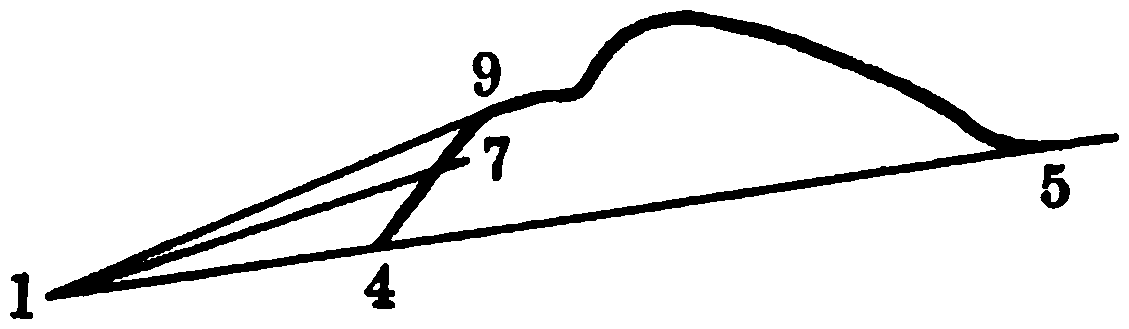
\includegraphics[width=\linewidth,height=32mm,keepaspectratio]{fig_assets/fig11_src_clean_x8.png}
\end{minipage}\hfill
\begin{minipage}[c]{0.49\linewidth}\centering
\end{minipage}
\end{center}

 so hat man nach (61), indem man Längen gerader Strecken durch $\overline{J}$ bezeichnet,
\[
\overline{J}_{17}+J_{75}>\overline{J}_{19}+J_{95},
\]
die Grösse $J_{13}+J_{23}$ nimmt also ab, und hat zu Anfang einen grösseren Werth als zu Ende der Bewegung des Punktes 2.



\noindent\textbf{Aufgabe II (\S~9).} Die Grösse $\mathfrak{E}$ unterscheidet sich von der für die Aufgabe I erhaltenen nur um den positiven Factor $y$, die \textsc{Weierstrass}'sche Bedingung des starken Minimums ist also erfüllt.

Führen wir die hyperbolischen Functionen ein und setzen
\[
\Cof z=\frac{e^z+e^{-z}}{2},\quad
\Sin z=\frac{e^z-e^{-z}}{2},\quad
\Tg z=\frac{1}{\Ctg z}=\frac{\Sin z}{\Cof z},
\]
wobei die Gleichungen
\[
\Cof^2z-\Sin^2z=1,\quad
d\Cof z=\Sin z\,dz,\quad
d\Sin z=\Cof z\,dz,
\]
\[
d\Tg z=\frac{dz}{\Cof^2z},\quad
d\Ctg z=\frac{-dz}{\Sin^2z}
\]
bestehen, so gelten für die Extremalen die Gleichungen
\begin{equation}\tag{62}
y=a\Cof\frac{x-b}{a},\quad
p=\Sin\frac{x-b}{a}.
\end{equation}
Wir fassen speciell diejenigen Extremalen ins Auge, welche die gegebene Curve $\mathfrak{C}_0$ transversal, d.~h. rechtwinkelig (\S~11) schneiden. Die Gleichung dieser Curve sei
\[
y_0=f(x_0);
\]
dann sind die Constanten der senkrecht schneidenden Extremalen den Gleichungen
\[
y_0=a\Cof\frac{x_0-b}{a},\quad
1+p_0f'(x_0)=0
\]
unterworfen, oder, wenn
\[
u=\frac{x-b}{a},\quad u_0=\frac{x_0-b}{a}
\]
gesetzt wird,
% src-pdfpage=0106
% src-break=0106
\begin{equation}\tag{63}
f(x_0)=a\Cof u_0,\quad
1+f'(x_0)\Sin u_0=0.
\end{equation}
Differenzirt man hier und in der ersten Gleichung (62) nach $x,x_0,a,b$, so ergiebt sich
\[
dy=\Sin u\,dx+0\,dx_0+(\Cof u-u\Sin u)\,da-\Sin u\,db,
\]
\[
0=[\Sin u_0-f'(x_0)]\,dx_0+(\Cof u_0-u_0\Sin u_0)\,da-\Sin u_0\,db,
\]
\begin{equation}\tag{64}
0=
\left[\frac{f'(x_0)}{a}\Cof u_0+f''(x_0)\Sin u_0\right]dx_0
-\frac{f'(x_0)}{a}u_0\Cof u_0\,da
-\frac{f'(x_0)}{a}\Cof u_0\,db.
\end{equation}
Die Determinante der mit $da,db$ behafteten Glieder in den letzten beiden Gleichungen ist
\[
M=
\frac{f'(x_0)\Cof u_0}{a}
\begin{vmatrix}
\Cof u_0-u_0\Sin u_0 & -\Sin u_0\\
-u_0 & -1
\end{vmatrix}
=
\frac{f'(x_0)\Cof^2u_0}{-a},
\]
also von Null verschieden, wenn, was wir voraussetzen wollen, die Curve $\mathfrak{C}_0$ an der betrachteten Stelle nicht der $x$-Axe parallel läuft. Man kann daher $a$ und $b$ als reguläre Functionen von $x_0$ aus den Gleichungen (63) bestimmt denken, und erhält $y$ durch $x$ und $x_0$ ausgedrückt. Da ferner $y$ längs jeder Kettenlinie eine eindeutige Function von $x$ ist, kann man $t=x$ setzen; für die Extremalenschar, welche $\mathfrak{C}_0$ senkrecht schneidet, erhält man daher
\[
\Delta=\frac{\partial(x,y)}{\partial(x,x_0)}=\frac{\partial y}{\partial x_0},\quad
dy=p\,dx+\Delta\,dx_0.
\]
Aus den Gleichungen (64) ergiebt sich aber, indem man $da$ und $db$ durch eine elementare Rechnung eliminirt,
\[
M\,dy=M\Sin u\,dx+dx_0(\ldots),
\]
wobei der Factor von $dx_0$ die Determinante der Coëfficienten von $dx_0,da,db$ in den citirten Gleichungen ist; man hat daher
\[
M\Delta=
\begin{vmatrix}
0 & \Cof u-u\Sin u & -\Sin u\\
\Sin u_0-f'(x_0) & \Cof u_0-u_0\Sin u_0 & -\Sin u_0\\
\dfrac{f'(x_0)}{a}\Cof u_0+f''(x_0)\Sin u_0 &
-\dfrac{f'(x_0)}{a}u_0\Cof u_0 &
-\dfrac{f'(x_0)}{a}\Cof u_0
\end{vmatrix}.
\]
So lange dieser Ausdruck nicht verschwindet, liefert der im Punkte 0 die Linie $\mathfrak{C}_0$ senkrecht schneidende Extremalenbogen 02 ein starkes Minimum der Rotationsfläche, verglichen mit allen Curven, die $\mathfrak{C}_0$ mit dem Punkte 2 verbinden.

Berücksichtigt man ferner die zweite Gleichung (63) und setzt
% src-pdfpage=0107
% src-break=0107
\[
\frac{f''(x_0)}{\left(\sqrt{1+[f'(x_0)]^2}\right)^3}
=
\frac{f''(x_0)}{(1+\Sin^{-2}u_0)^{3/2}}
=
f''(x_0)\Tg^3u_0
=
\frac{1}{r},
\]
so ist $|r|$ der Krümmungsradius der Curve $\mathfrak{C}_0$ und man kann schreiben
\[
M\Delta
=
-\frac{\Cof^3u_0}{r\Sin^2u_0}
\begin{vmatrix}
\Cof u-u\Sin u & \Sin u\\
\Cof u_0-u_0\Sin u_0 & \Sin u_0
\end{vmatrix}
\]
\[
\qquad
+\frac{\Cof^2u_0}{y_0\Sin u_0}
\begin{vmatrix}
0 & \Cof u-u\Sin u & -\Sin u\\
\Cof u_0\Ctg u_0 & \Cof u_0-u_0\Sin u_0 & -\Sin u_0\\
-1 & u_0 & 1
\end{vmatrix}.
\]
Geht $\mathfrak{C}_0$ in einen unendlich kleinen Kreis über, so wird $r=0$, und die Gleichung $\Delta=0$ erfordert
\[
\begin{vmatrix}
\Cof u-u\Sin u & \Sin u\\
\Cof u_0-u_0\Sin u_0 & \Sin u_0
\end{vmatrix}
=0,\quad
\Ctg u-u=\Ctg u_0-u_0
\]
oder
\[
\frac{y}{p}-x=\frac{y_0}{p_0}-x_0;
\]
diese Gleichung drückt aus, dass die Tangenten der Extremale in den Punkten 0 und $(x,y)$ sich auf der $x$-Axe schneiden. So lange dies also für keine zwei Tangenten des Bogens 02 eintritt, bilden die durch den Punkt 0 gehenden Extremalen ein Feld jedes Bogens 12, der ein Theil von 02 ist. Da nun die Punkte 0 und 1 einander beliebig nahe rücken können, so folgt, dass jeder Bogen der Extremale, von dessen Tangenten keine zwei sich auf der $x$-Axe schneiden, ein Extremum bei festen Endpunkten liefert.

Im allgemeinen Falle einer endlichen Krümmung der Curve $\mathfrak{C}_0$ hat die Gleichung $\Delta=0$ die Form
\[
A(\Cof u-u\Sin u)+B\Sin u=0,
\]
wobei $A$ und $B$ allein von $u_0,y_0$ und $1:r$ abhängen, und in Bezug auf die letzte Grösse linear sind. Ist $A$ von Null verschieden, so kann man die Gleichung schreiben
\begin{equation}\tag{65}
\Ctg u-u+\frac{B}{A}=0;
\end{equation}
die linke Seite hat dann die Ableitung
\[
-\frac{1}{\Sin^2u}-1,
\]
nimmt also bei wachsenden Werthen von $u$ beständig ab. Nun findet man leicht
% src-pdfpage=0108
% src-break=0108
\[
\Ctg(\mp\infty)=\mp1,\quad \Ctg(\pm0)=\pm\infty,
\]
die Gleichung (65) hat also eine einzige endliche Wurzel, wenn
\[
|B|>|A|,
\]
anderenfalls hat sie keine Wurzel. Fixirt man ferner $u_0$ und $y_0$, d.~h. hält man den Punkt 0 und die Richtung der Curve $\mathfrak{C}_0$ fest, so kann über die Krümmung dieser Curve so verfügt werden, dass $B:A$ einen gegebenen Werth erhält; man kann also durch passende Wahl von $r$ immer erreichen, dass die zur Curve $\mathfrak{C}_0$ senkrechte Extremale in einem gegebenen Punkte 2 aufhört, mit Sicherheit ein Minimum im Vergleich zu den die Curve $\mathfrak{C}_0$ mit dem Punkte 2 verbindenden Curven zu liefern.

\noindent\textbf{Aufgabe IV (\S~9).} Ist $\Omega$ eine beliebige, in der $wy$-Ebene vom Punkte $w=y=0$ aus durch die Halbebene $y>0$ zur Linie $y$ wieder herabsteigende Linie mit den Stetigkeitseigenschaften der ebenso bezeichneten in \S~17, und hat der Parameter $\tau$ im Coordinatenanfangspunkte den Werth $\tau_0$, so ist, indem $w$ für das Zeichen $u$ des \S~9 gesetzt wird,
\begin{equation}\tag{66}
x=\int_{\tau_0}^{\tau}
y\sqrt{\left(\frac{dw}{d\tau}\right)^2+\left(\frac{dy}{d\tau}\right)^2}\,d\tau
\end{equation}
mit positiver Quadratwurzel, also sicher
\begin{equation}\tag{67}
x\geq \int_{\tau_0}^{\tau}y\frac{dy}{d\tau}\,d\tau,\quad
x\geq \frac{y^2}{2}.
\end{equation}
Das Gleichheitszeichen gilt nur dann, wenn zwischen $\tau_0$ und $\tau$ immer
\[
\frac{dw}{d\tau}=0
\]
ist. Die entsprechende Curve $\Omega_1$ in der $xy$-Ebene liegt also im ersten Quadranten $(x>0,y>0)$ und im Inneren, d.~h. auf der concaven Seite der Parabel
\begin{equation}\tag{68}
y^2=2x.
\end{equation}
Das Innere dieser Parabel wird durch die vom Punkte $0(x=y=0)$ ausgehenden Extremalen
\begin{equation}\tag{69}
1-\frac{x}{a^2}
=
\sqrt{1-\left(\frac{y}{a}\right)^2},\quad
\frac{x^2}{a^2}=2x-y^2
\end{equation}
genau einfach bedeckt, da sich aus diesen Gleichungen ein einziger positiver Werth von $a^2$ ergiebt, wenn $x,y$ gegeben sind und
% src-pdfpage=0109
% src-break=0109
$2x-y^2$ positiv ist. Geht die Curve $\Omega$ zuerst ein Stück weit parallel der $y$-Axe, so hat die Curve $\Omega_1$ ein entsprechendes Stück 01 mit der Parabel (68) gemein, welches für $J$ den Beitrag Null ergiebt; ist daher 3 der Endpunkt der Curve $\Omega_1$, also $y_3=0$, so hat man längs derselben
\begin{equation}\tag{70}
J_{03}=J_{13}.
\end{equation}
Hat die Curve $\Omega_1$ die Parabel einmal verlassen, so kann sie dieselbe nicht wieder erreichen, da dann $dw:d\tau$ wenigstens streckenweise von Null verschieden ist, in der Relation (67) also das Gleichheitszeichen nicht mehr gelten kann.

Die Ellipsen (69) bilden ein Feld innerhalb derjenigen Hälfte der Parabel (68), für welche $y>0$; denn hier ist
\[
x=\xi=t,\quad
y=\eta=\sqrt{2t-\left(\frac{t}{a}\right)^2},
\]
woraus sich ergiebt
\[
\Delta=\frac{\partial(\xi,\eta)}{\partial(t,a)}
=\frac{\partial y}{\partial a}
=
\frac{t^2}{a^3}\left(2t-\frac{t^2}{a^2}\right)^{-1/2},
\]
ein Werth, der offenbar von Null verschieden ist. Man findet ferner, wenn $a$ und die Quadratwurzel positiv, und 2 irgend ein Punkt des betrachteten Gebietes ist:
\begin{equation}\tag{71}
u=\overline{J}_{02}
=
\int_0^x y\sqrt{1-y^2p^2}\,dx
=
\int_0^x\frac{y^2}{a}\,dx
=
\frac{x^2}{a}-\frac{x^3}{3a^3}
\end{equation}
und verificirt leicht, indem man $dy$ mittelst der Gleichung (69) durch $dx$ und $da$ ausdrückt, und $x',y',p$ auf die Extremalen des Feldes bezieht, die Gleichungen
\[
F_{x'}=a,\quad F_{y'}=-ay^2p,\quad du=F_{x'}dx+F_{y'}dy;
\]
daraus folgt, wenn der Punkt 2 längs der Curve $\Omega_1$ von 1 bis 3 läuft:
\[
d(\overline{J}_{02}+J_{23})=\mathfrak{E}\,d\tau,
\]
und man hat nach der Formel (58), wenn $D x$ und $\bar{p}$ sich auf die Linie $\Omega_1$, $p$ auf die Extremale bezieht,
\[
\mathfrak{E}d\tau
=
y\left\{
\frac{1-y^2p\bar{p}}{\sqrt{1-y^2p^2}}
-
\sqrt{1-y^2\bar{p}^2}
\right\}D x,
\]
wobei die Quadratwurzel im Nenner positiv ist. Nun liegt für jede in Betracht kommende Richtung die Grösse
% src-pdfpage=0110
% src-break=0110
\[
y\frac{dy}{dx}
=
\frac{dy}{\sqrt{dy^2+dw^2}}
\]
zwischen den Grenzen $\pm1$ und erreicht diese selbst auf der Extremale des Feldes nur für $y=0$; so lange also $y$ nicht verschwindet, ist $y^2p\bar{p}$ ein echter Bruch und die Grösse $1-y^2p\bar{p}$ positiv. Dasselbe gilt, da $y$ und $D x$ positiv sind, von $\mathfrak{E}d\tau$ offenbar, wenn $\sqrt{1-y^2\bar{p}^2}$ negativ ist; hat diese Grösse einen positiven Werth, so folgt aus der allgemeinen Ungleichung
\[
(1-\alpha\beta)^2\geq(1-\alpha^2)(1-\beta^2),
\]
dass $\mathfrak{E}d\tau$ nie negativ ist und nur verschwindet, wenn $p=\bar{p}$, d.~h. nur in ordentlicher Weise, da das auf die Extremale bezügliche Differential $dx$ ebenso wie $D x$ positiv ist. Besteht die Gleichung
\[
1-y^2\bar{p}^{\,2}=0,
\]
so ist zwar der in $x,y$ ausgedrückte Integrand des Integrals $J$ singulär; die ursprüngliche Definition
\[
J=\int y^2\frac{dw}{d\tau}\,d\tau
=
\int y\sqrt{1-y^2\bar{p}^{\,2}}\frac{dx}{d\tau}\,d\tau
\]
lehrt aber, dass $J_{23}$ trotzdem eine Function $\varphi(\tau)$ im Sinne des \S~17 bleibt. Die Grösse $dJ_{23}$ verschwindet in diesem Falle; $du$ hat den Ausdruck
\[
du=a(1-y^2p\bar{p})\,dx,
\]
bleibt also positiv. Wenn daher $\mathfrak{E}$ auf der Curve $\Omega_1$ nicht überall ordentlich verschwindet, d.~h. wenn diese Curve nicht mit einer der Extremalen (69) zusammenfällt, so wächst die Grösse $\overline{J}_{02}+J_{23}$ beständig, so lange der Punkt 2 zwischen 1 und 3 liegt; in diesen Punkten selbst gelten freilich unsere Betrachtungen nicht mehr. Nähert sich der Punkt 2 den Lagen 1 und 3, so convergirt jene Grösse gegen die Grenzwerthe $J_{13}$ und $\overline{J}_{03}$; denn wenn der Punkt 2 sich einer bestimmten Stelle der Parabel annähert, ergeben die Formeln (69), (71)
\[
\lim\frac{x}{a}=0,\quad \lim u=\lim\overline{J}_{02}=0.
\]
Aus dem Verhalten der Grösse $\mathfrak{E}$ ergiebt sich also mit Berücksichtigung der Relation (70), wenn $\Omega_1$ nicht eine der Curven (69) ist,
% src-pdfpage=0111
% src-break=0111
\[
\overline{J}_{03}>J_{13},\quad
\overline{J}_{03}>J_{013},
\]
d.~h. die Kugel hat grösseres Volumen als der durch Rotation der Curve $\Omega$ entstandene Körper von derselben Oberfläche.

% src-pdfpage=0111 portion=lower
% unit: sec24 source=kneser_lvr_1900_archiveorg.pdf#p0111 authorial=true
\begin{center}{\large \S~24.}\end{center}

Geht man die Curve $\mathfrak{C}$ vom Punkte 0 aus in der Richtung wachsender $t$ entlang, so sei 6 der erste Punkt, in welchem, nachdem man 0 verlassen hat, die Grösse $\Delta$ verschwindet. Wir setzen voraus, dass dies eher eintrete, als die Functionen $\xi$ und $\eta$ ihre vorausgesetzten Eigenschaften längs der Curve $\mathfrak{C}$ verlieren, so dass 6 noch ein regulärer Punkt dieser Curve ist, in dessen Umgebung durch Ungleichungen
\[
|t-t_6|<\varepsilon,\quad |a-a_0|<\varepsilon
\]
für die Grössen $t,a$ ein Gebiet definirt wird, innerhalb dessen die Functionen $\xi,\eta,F(\xi,\eta,\xi_t,\eta_t)$ regulär bleiben und die Grösse $\xi_t^2+\eta_t^2$ von Null verschieden ist. Die entsprechenden Punkte $(x,y)$, welche durch die Gleichungen
\[
x=\xi(t,a),\quad y=\eta(t,a)
\]
bestimmt werden, gehören dem Felde eines Theils der Curve $\mathfrak{C}$ nicht mehr an, da sie im Allgemeinen gewisse Gebiete der Ebene doppelt bedecken. Nimmt, wie früher, im Punkte 0 die Curve $\mathfrak{C}_0$ ihren Anfang, welche von den Extremalen des Feldes transversal geschnitten wird, so nennen wir 6 den extremalen Brennpunkt der Curve $\mathfrak{C}_0$ auf der Extremale $\mathfrak{C}$; zieht die Curve $\mathfrak{C}_0$ sich in den Punkt 0 zusammen, durch welchen dann auch alle Extremalen des Feldes gehen, so heissen 0 und 6 conjugirte Punkte oder ausführlicher extremal conjugirte Punkte. Z.~B. sind nach \S~23 bei der Aufgabe II conjugirte Punkte dadurch charakterisirt, dass ihre Tangenten sich auf der $x$-Axe schneiden; der extremale Brennpunkt einer beliebigen Curve $\mathfrak{C}_0$ wird durch die leicht discutirbare Gleichung (65) definirt.

Wichtige Eigenschaften der conjugirten und Brennpunkte beruhen darauf, dass die Grösse $\Delta$ einer linearen Differentialgleichung genügt, welche allein durch die Extremale $\mathfrak{C}$ bestimmt wird. Zu dieser Gleichung führt die geometrische Bedeutung der Grösse $\Delta$, welche aus folgender Betrachtung erkannt wird. Es seien
% src-pdfpage=0112
% src-break=0112
\begin{equation}\tag{72}
\begin{aligned}
x&=\xi(t,a),\quad y=\eta(t,a),\\
\bar x&=\xi(t,a+\delta a),\quad \bar y=\eta(t,a+\delta a)
\end{aligned}
\end{equation}
zwei benachbarte Extremalen des Feldes und liege der Punkt $(\bar x,\bar y)$ auf der Normalen der ersten Curve im Punkte $(x,y)$. Die Richtungscosinus dieser Geraden sind
\[
X=\frac{-y'}{\sqrt{x'^2+y'^2}},\quad Y=\frac{x'}{\sqrt{x'^2+y'^2}};
\]
nimmt man die Quadratwurzeln positiv, so beziehen sich diese Grössen auf diejenige Richtung, welche zur Richtung wachsender $t$ so liegt, wie die $+y$-Axe zur $+x$-Axe. Die Gleichung der Normale ist
\[
(\bar x-x)x'+(\bar y-y)y'=0;
\]
die Gleichungen (72) kann man schreiben
\[
\bar x-x-\{\xi_t(\tau-t)+\xi_a\delta a+[\tau-t,\delta a]_2\}=0,
\]
\[
\bar y-y-\{\eta_t(\tau-t)+\eta_a\delta a+[\tau-t,\delta a]_2\}=0,
\]
wobei die Grössen $\xi_t,\xi_a\ldots$ für das Argumentsystem $t,a$ zu nehmen sind. Die Functionaldeterminante der linken Seiten dieser drei Gleichungen nach $\bar x,\bar y,\tau$ ist, wenn für diese $\bar x,\bar y,t$ gesetzt wird:
\[
\begin{vmatrix}
x'&y'&0\\
1&0&-\xi_t\\
0&1&-\eta_t
\end{vmatrix}=x'^2+y'^2,
\]
also von Null verschieden; man kann daher die Grössen $\bar x-x$, $\bar y-y$, $\tau-t$ nach $\delta a$ entwickeln, wobei die linearen Glieder dieselben sind, wie wenn die Gleichungen jene drei Differenzen nur streng linear enthielten; somit folgt
\[
\bar x-x=-\frac{\eta_t\Delta\delta a}{\xi_t^2+\eta_t^2}+[\delta a]_2,\quad
\bar y-y=\frac{\xi_t\Delta\delta a}{\xi_t^2+\eta_t^2}+[\delta a]_2,
\]
oder, wenn
\begin{equation}\tag{73}
\omega=\frac{\Delta\delta a}{\sqrt{\xi_t^2+\eta_t^2}}
\end{equation}
gesetzt wird,
\[
\bar x-x=X\omega+[\delta a]_2,
\quad
\bar y-y=Y\omega+[\delta a]_2;
\]
$\omega$ ist also der Normalabstand der beiden Extremalen, wenn $\delta a$ unendlich klein wird, positiv oder negativ genommen, je nachdem die Richtung zum Punkte $(\bar x,\bar y)$ hin mit der oben definirten Normalrichtung übereinstimmt oder nicht.

% src-pdfpage=0113
% src-break=0113
Nun beschreibt der durch die Gleichungen (72) definirte Punkt $(\bar x,\bar y)$ bei willkürlich festgelegtem Werth von $\delta a$ eine Extremale; sind wie in \S~4 die Gleichungen einer solchen
\[
P=0,\quad Q=0,
\]
so kann man in ihnen $\bar x,\bar y$ für $x,y$ substituiren und nach $\delta a$ differenziren; setzt man sodann $\delta a=0$, so ergiebt z.~B. die erste Gleichung
\[
\frac{\partial P}{\partial x}\frac{\partial\bar x}{\partial\delta a}
+\frac{\partial P}{\partial x'}\frac{\partial\bar x'}{\partial\delta a}
+\frac{\partial P}{\partial x''}\frac{\partial\bar x''}{\partial\delta a}
+\frac{\partial P}{\partial y}\frac{\partial\bar y}{\partial\delta a}+\cdots=0.
\]
Dies Resultat kann auch in folgender Weise ausgedrückt werden: es gelten die Gleichungen
\[
\delta P=0,\quad \delta Q=0,
\]
wenn man setzt
\begin{equation}\tag{74}
\delta x=\omega X,
\quad
\delta y=\omega Y;
\end{equation}
letztere Gleichungen definiren, wie wir sagen wollen, eine Normalvariation. Da nämlich offenbar bis auf Glieder $[\delta a]_2$ die Gleichungen
\[
\delta a\frac{\partial\bar x}{\partial\delta a}=\omega X,
\quad
\delta a\frac{\partial\bar y}{\partial\delta a}=\omega Y
\]
gelten, so kann man die Operationen
\[
\delta,\quad \delta a\frac{\partial}{\partial\delta a}
\]
bei der Voraussetzung (74) als identisch betrachten. Um die angedeuteten Rechnungen durchzuführen, gehen wir von den Identitäten
\[
P=F_x-\frac{dF_{x'}}{dt},\quad
\delta P=\delta F_x-\frac{d\delta F_{x'}}{dt}
\]
aus; letztere ergiebt leicht
\[
\begin{aligned}
\delta P={}&\left(F_{xx}-\frac{dF_{xx'}}{dt}\right)\delta x
+\left(F_{xy}-\frac{dF_{x'y}}{dt}\right)\delta y\\
&-\frac{d}{dt}(F_{x'x'}\delta x'+F_{x'y'}\delta y')
+(F_{xy'}-F_{yx'})\delta y'
\end{aligned}
\]
und analog findet man
\[
\begin{aligned}
\delta Q={}&\left(F_{yx}-\frac{dF_{xy'}}{dt}\right)\delta x
+\left(F_{yy}-\frac{dF_{yy'}}{dt}\right)\delta y\\
&-\frac{d}{dt}(F_{y'x'}\delta x'+F_{y'y'}\delta y')
+(F_{yx'}-F_{xy'})\delta x'.
\end{aligned}
\]
% src-pdfpage=0114
% src-break=0114
Jetzt werde die in \S~16 definirte Grösse $F_1$ eingeführt und berücksichtigt, dass für die Normalvariation (74)
\[
y'\delta x'-x'\delta y'=-\omega'\sqrt{x'^2+y'^2};
\]
setzt man noch
\[
F^1=F_1(x'^2+y'^2),
\]
\[
\begin{aligned}
F_2={}&\left(F_{xx}-\frac{dF_{xx'}}{dt}\right)X^2
+\left(2F_{xy}-\frac{dF_{x'y}}{dt}-\frac{dF_{y'x}}{dt}\right)XY\\
&+\left(F_{yy}-\frac{dF_{yy'}}{dt}\right)Y^2
+(F_{xy'}-F_{yx'})(XY'-YX'),
\end{aligned}
\]
so ergiebt sich aus den hingeschriebenen Werthen von $\delta P$ und $\delta Q$
\[
X\delta P+Y\delta Q
=F_2\omega-X\frac{d}{dt}(F^1X\omega')-Y\frac{d}{dt}(F^1Y\omega');
\]
mit Berücksichtigung der Identitäten
\[
X^2+Y^2=1,\quad XX'+YY'=0
\]
folgt hieraus
\begin{equation}\tag{75}
X\delta P+Y\delta Q=F_2\omega-\frac{d}{dt}\left(F^1\frac{d\omega}{dt}\right),
\end{equation}
und dies ist, was wir später benutzen, eine reine Identität bei der Voraussetzung (74) und beliebigen Werthen von $\omega$.

Nimmt man für $\omega$ den Werth (73), so ergiebt sich
\[
X\delta P+Y\delta Q=0,
\quad
F_2\omega-\frac{d}{dt}\left(F^1\frac{d\omega}{dt}\right)=0.
\]
Wenn daher längs des betrachteten Stückes der Extremale
\[
x=\xi(t,a),\quad y=\eta(t,a),
\]
etwa längs des Bogens 06 die Grösse $F_1$ von Null verschieden ist, so genügt $\omega$ einer linearen Differentialgleichung, deren Coefficienten, wenn man sie in der Form
\[
\omega''+M\omega'+N\omega=0
\]
schreibt, von $t_0$ bis $t_6$ reguläre Functionen von $t$ sind. Die Grösse $\omega$ kann daher, wenn sie nicht identisch verschwindet, nicht zugleich mit ihrer Ableitung nach $t$ verschwinden und der Gleichung (73) zufolge gilt dasselbe von $\Delta$, so dass jedenfalls
\[
\Delta_t(t_6,a_0)\gtrless0.
\]

% src-pdfpage=0115
% src-break=0115
% unit: sec25 source=kneser_lvr_1900_archiveorg.pdf#p0115 authorial=true
\begin{center}{\large \S~25.}\end{center}

Die erhaltene Ungleichung zeigt, dass man die Gleichung
\begin{equation}\tag{76}
\Delta(t,a)=0,
\end{equation}
der das Werthsystem $t_6,a_0$ genügt, in der Umgebung desselben nach $t$ auflösen kann; schreibt man diese Gleichung in der Form
\[
\Delta_t(t_6,a_0)(t-t_6)+\Delta_a(t_6,a_0)(a-a_0)+[a-a_0,t-t_6]_2=0,
\]
so ist klar, dass man aus ihr erhält
\[
t-t_6=-\frac{\Delta_a}{\Delta_t}(a-a_0)+[a-a_0]_2.
\]
Substituirt man diesen Werth in die Entwickelungen von $\xi$ und $\eta$ für die Umgebung der Stelle 6, so wird durch die Gleichungen
\begin{equation}\tag{77}
\begin{aligned}
x&=\xi(t,a)=x_6+[a-a_0]_1,\\
y&=\eta(t,a)=y_6+[a-a_0]_1
\end{aligned}
\end{equation}
eine Curve definirt, welche den Punkt 6 enthält und durch $\mathfrak{C}$ bezeichnet werde (Fig.~12). Sie ist in allen Punkten, welche hinreichend kleinen, nicht verschwindenden Werthen von $|a-a_0|$ entsprechen, regulär; im Punkte 6 selbst kann sie einen Rückkehrpunkt darbieten oder auch speciell sich ganz in diesem Punkt zusammenziehen. Letzteres geschieht in dem Falle, dass die Potenzreihen $[a-a_0]_1$ in den Gleichungen (77) identisch verschwinden. Die Incremente der Coordinaten beim Fortgang längs dieser Curve haben folgenden Ausdruck

% unit: fig12 source=kneser_lvr_1900_archiveorg.pdf#p0115 authorial=true type=hq_sourcecrop
\begin{center}
{\small Fig.~12.}\par\vspace{1mm}
\begin{minipage}[c]{0.47\linewidth}\centering
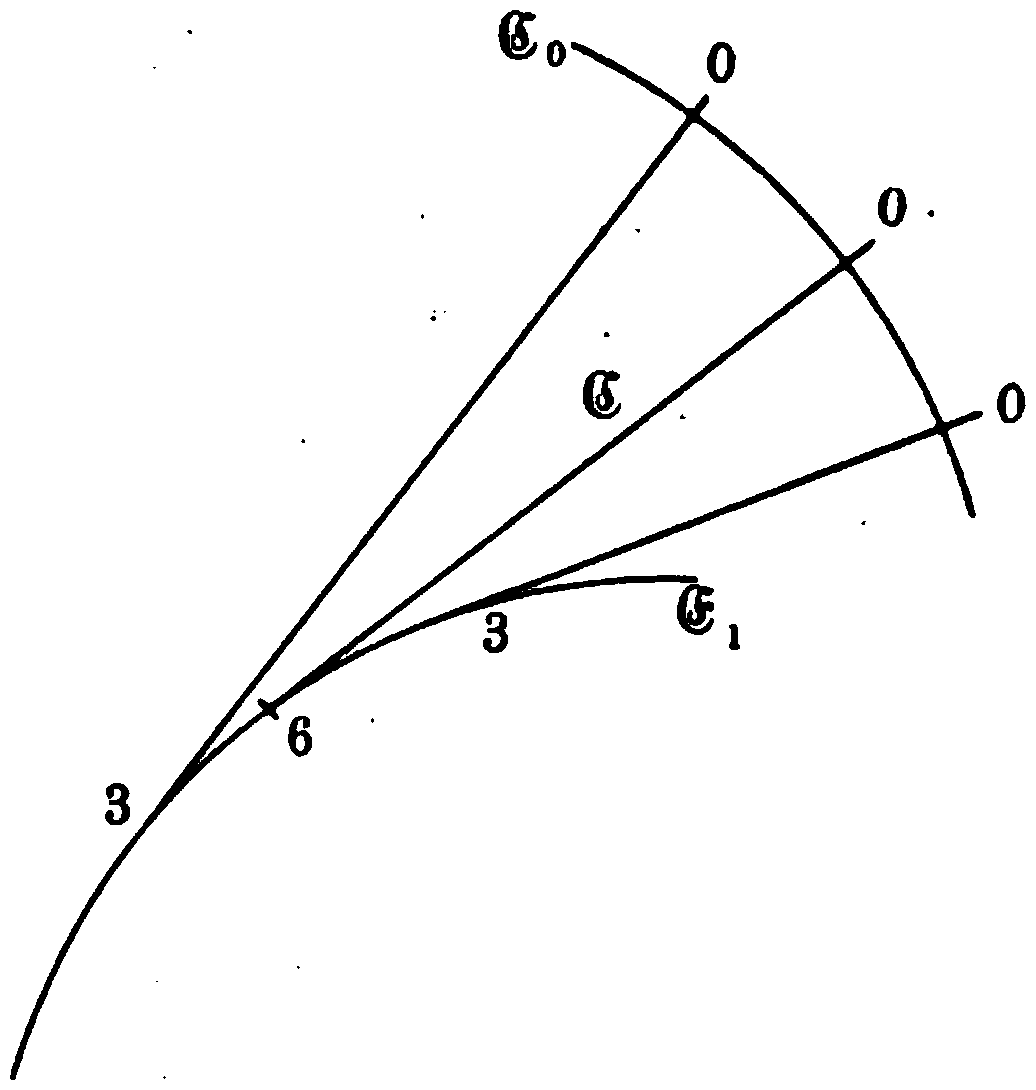
\includegraphics[width=\linewidth,height=38mm,keepaspectratio]{fig_assets/fig12_src_clean_x8.png}
\end{minipage}\hfill
\begin{minipage}[c]{0.49\linewidth}\centering
\end{minipage}
\end{center}
\[
Dx=\frac{dx}{da}\,da=\left(\xi_a+\xi_t\frac{dt}{da}\right)da
=\frac{\xi_t\Delta_a-\xi_a\Delta_t}{-\Delta_t}\,da,
\]
\[
Dy=\frac{dy}{da}\,da=\left(\eta_a+\eta_t\frac{dt}{da}\right)da
=\frac{\eta_t\Delta_a-\eta_a\Delta_t}{-\Delta_t}\,da;
\]
da nun $\xi_t$ und $\eta_t$ nicht zugleich verschwinden, so kann die Gleichung (76) in einer der Formen
\[
\eta_a=\frac{\eta_t\xi_a}{\xi_t},\quad \xi_a=\frac{\xi_t\eta_a}{\eta_t}
\]
% src-pdfpage=0116
% src-break=0116
geschrieben, und hieraus eine der Doppelgleichungen
\begin{equation}\tag{78}
\begin{aligned}
Dy&=\frac{\eta_t}{\xi_t}\left(\xi_a+\xi_t\frac{dt}{da}\right)da=\frac{\eta_t}{\xi_t}Dx,\\
Dx&=\frac{\xi_t}{\eta_t}\left(\eta_a+\eta_t\frac{dt}{da}\right)da=\frac{\xi_t}{\eta_t}Dy
\end{aligned}
\end{equation}
gefolgert werden; die Curve $\mathfrak{C}$ wird also in jedem ihrer Punkte, welche von 6 hinreichend wenig entfernt sind, von derjenigen Extremale des Feldes berührt, welche zu demselben Werthe von $a$ wie der betrachtete Punkt gehört. Die Curve ist also Enveloppe der Extremalen des Feldes, und die Existenz einer solchen unter den eingeführten Voraussetzungen erwiesen.

Längs der Curve $\mathfrak{C}$ nähert man sich nun dem zu $a=a_0$ gehörigen Punkte 6, wenn man $a$ um $da$ vermehrt und annimmt
\begin{equation}\tag{79}
(a-a_0)da<0.
\end{equation}
Wenn ferner $\xi_t$ im Punkte 6 nicht verschwindet und
\begin{equation}\tag{80}
\xi_t\frac{dx}{da}\bigg|^6(a-a_0)<0,
\quad
\left|\frac{dx}{da}\right|^6>0,
\end{equation}
so ist bei der Annahme (79)
\[
\xi_t\frac{dx}{da}\bigg|^6 da>0;
\]
bei dem durch die Relation (80) bestimmten Vorzeichen der Grösse $a-a_0$ haben daher die Grössen $\xi_t$ und $Dx$ dasselbe Vorzeichen, und stimmt der nach dem Punkte 6 hin gerichtete Fortgang längs der Curve $\mathfrak{C}$ überein mit der Richtung wachsender $t$ längs der berührenden Extremale. Diejenige Hälfte der Curve $\mathfrak{C}$, für welche die Ungleichung (80) gilt, nennen wir $\mathfrak{C}_1$; längs derselben hat man nach (78) die beiden Gleichungen
\begin{equation}\tag{81}
Dx=\alpha\xi_tdt=\alpha dx,
\quad
Dy=\alpha\eta_tdt=\alpha dy,
\end{equation}
wobei $\alpha$ positiv ist. Zweifelhaft wird die Existenz eines solchen Bogens $\mathfrak{C}_1$ nur in dem Falle
\[
\frac{dx}{da}\bigg|^6=0,
\quad
\left.\xi_t\Delta_a-\xi_a\Delta_t\right|^6=0,
\]
in welchem auch die Gleichung
\[
\Delta_t\frac{dy}{da}\bigg|^6=\eta_t\Delta_a-\eta_a\Delta_t
=\left.\eta_t\left(\Delta_a-\frac{\Delta_t\xi_a}{\xi_t}\right)\right|^6=0
\]
besteht. Dann hat möglicherweise (Fig.~13) die Curve $\mathfrak{C}$ im Punkte 6 einen Rückkehrpunkt; nur wenn beide Zweige vom
% src-pdfpage=0117
% src-break=0117
Punkte 6 in der Richtung fortgehen, welche auf der Curve $\mathfrak{C}$ wachsenden Werthen von $t$ entspricht, ist kein Bogen $\mathfrak{C}_1$ vorhanden. Wir bezeichnen dies als den Ausnahmefall.

% unit: fig13 source=kneser_lvr_1900_archiveorg.pdf#p0117 authorial=true type=hq_sourcecrop
\begin{center}
{\small Fig.~13.}\par\vspace{1mm}
\begin{minipage}[c]{0.47\linewidth}\centering
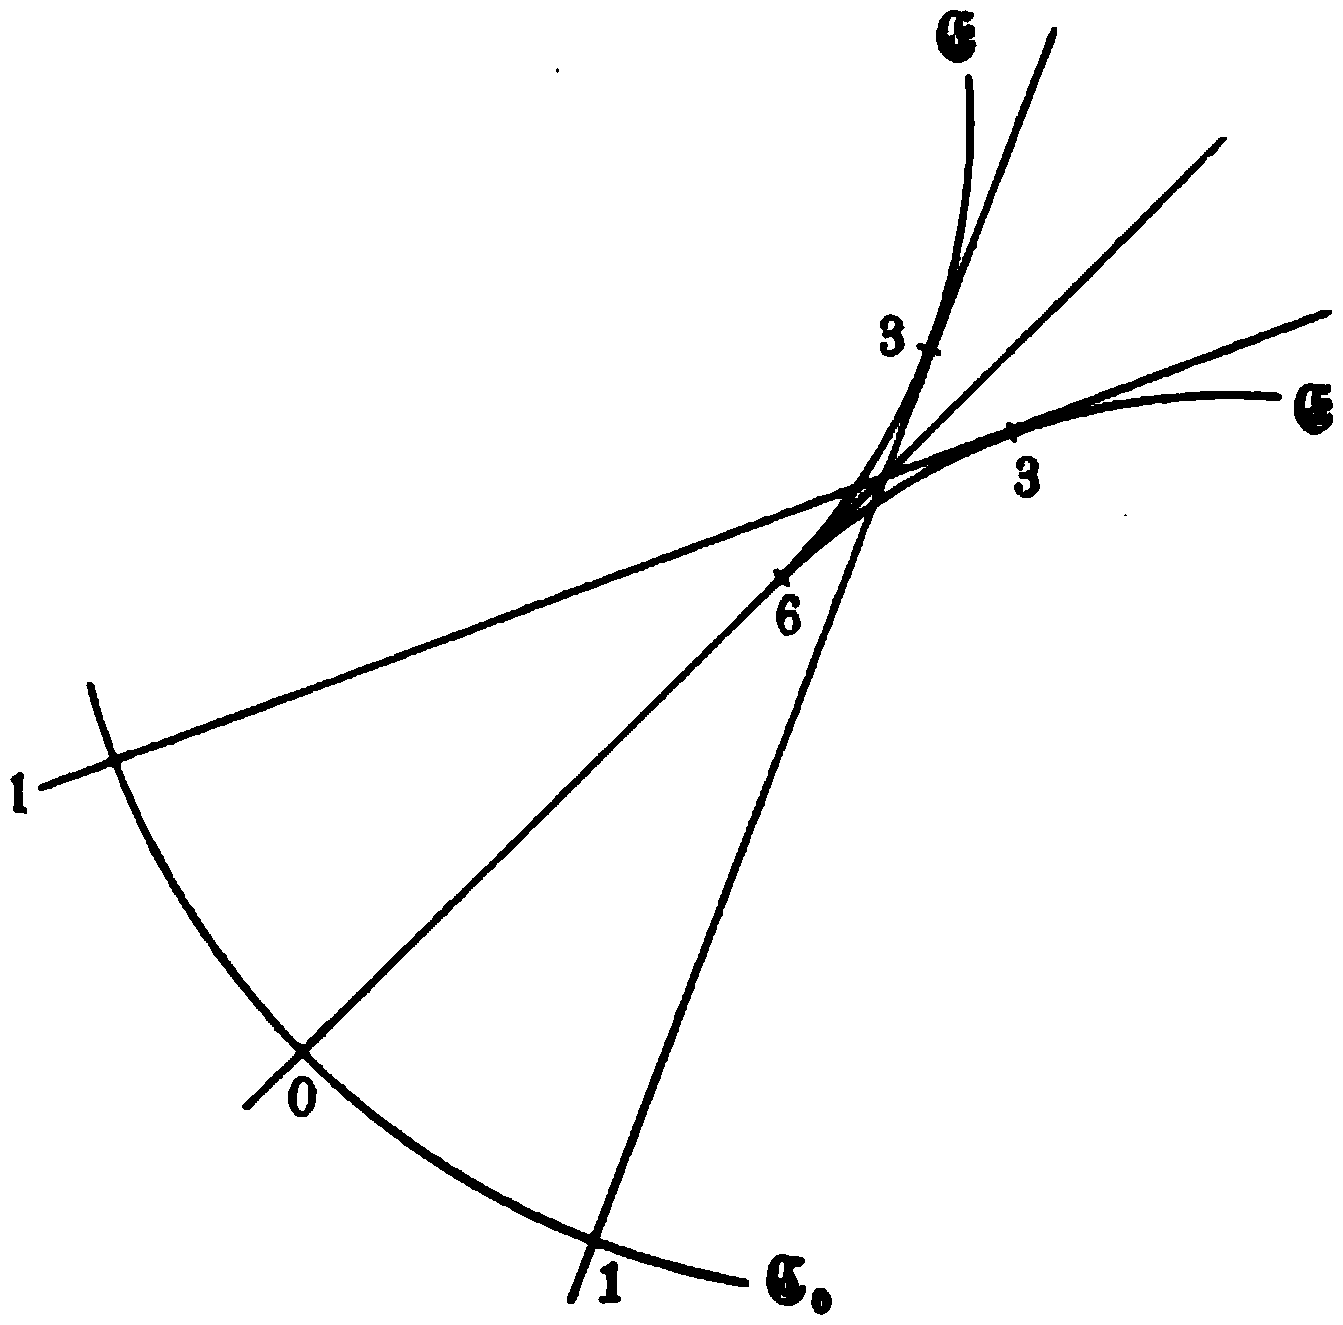
\includegraphics[width=\linewidth,height=38mm,keepaspectratio]{fig_assets/fig13_src_clean_x8.png}
\end{minipage}\hfill
\begin{minipage}[c]{0.49\linewidth}\centering
\end{minipage}
\end{center}

Wie früher sei 0 ein Punkt der Curve $\mathfrak{C}_0$ und 3 ein mit ihm auf derselben Extremale des Feldes liegender Punkt, auf den sich die Argumente $a$ und $t$ beziehen. Dann ist die Grösse
\[
u=\overline{J}_{03}=\int_0^3F(\xi,\eta,\xi_t,\eta_t)dt
\]
nicht nur, wie wir wissen, im Felde, sondern auch in demjenigen Gebiete $\mathfrak{B}'$ eine reguläre Function von $a$ und $t$, in welchem die Grössen $\xi,\eta,F(\xi,\eta,\xi_t,\eta_t)$ regulär bleiben. Die Gleichungen
\[
\frac{\partial u}{\partial a}=F_{x'}(\xi,\eta,\xi_t,\eta_t)\xi_a
+F_{y'}(\xi,\eta,\xi_t,\eta_t)\eta_a,
\]
\[
\frac{\partial u}{\partial t}=F(\xi,\eta,\xi_t,\eta_t),
\]
welche zunächst für das Feld abgeleitet sind, gelten daher auch im Gebiete $\mathfrak{B}'$, da in diesem ihre rechten wie linken Seiten reguläre Functionen von $a$ und $t$ bleiben. Speciell sei 3 ein Punkt der Curve $\mathfrak{C}$; dann hat man bei Fortgang längs derselben
\[
\begin{aligned}
du={}&F_{x'}(\xi,\ldots,\eta_t)(\xi_a da+\xi_tdt)
+F_{y'}(\xi,\ldots,\eta_t)(\eta_ada+\eta_tdt)\\
={}&F_{x'}(\xi,\ldots,\eta_t)Dx+F_{y'}(\xi,\ldots,\eta_t)Dy.
\end{aligned}
\]
Andererseits bilde man längs der Curve $\mathfrak{C}$ das Integral
\[
J_{36}=\int_3^6F(x,y,Dx,Dy),
\]
so dass das Zeichen $D$ der nach dem Punkte 6 hin gerichteten Bewegung längs der Curve $\mathfrak{C}$ entspricht. Dann ist
\[
dJ_{36}=-F(x,y,Dx,Dy)=-F(\xi,\eta,Dx,Dy).
\]
Diese Grösse ist der für $du$ erhaltenen entgegengesetzt, wenn man die Homogeneitätsgleichungen
% src-pdfpage=0118
% src-break=0118
\[
F_{x'}(\xi,\eta,\xi_t,\eta_t)=F_{x'}(\xi,\eta,Dx,Dy),
\]
\[
F_{y'}(\xi,\eta,\xi_t,\eta_t)=F_{y'}(\xi,\eta,Dx,Dy)
\]
anwenden kann, also wenn die Gleichungen (81) gelten und $\alpha$ positiv ist, so dass der Punkt 3 dem Bogen $\mathfrak{C}_1$ angehört. In diesem Falle hat man die Gleichungen
\[
\begin{aligned}
F_{x'}(\xi,\ldots,\eta_t)Dx+F_{y'}(\xi,\ldots,\eta_t)Dy
={}&F_{x'}(\xi,\eta,Dx,Dy)Dx\\
&+F_{y'}(\xi,\eta,Dx,Dy)Dy\\
={}&F(\xi,\eta,Dx,Dy),
\end{aligned}
\]
\[
du+dJ_{36}=d(\overline{J}_{03}+J_{36})=0.
\]
Da nun, wenn der Abstand der Punkte 3 und 6 unendlich klein wird und damit die Extremalen 03 und $\mathfrak{C}$ zusammenfallen, offenbar die Gleichung
\[
\lim(\overline{J}_{03}+J_{36})=\overline{J}_{06}
\]
gilt, so folgt allgemein
\begin{equation}\tag{82}
\overline{J}_{03}+J_{36}=\overline{J}_{06}.
\end{equation}
Zieht sich die Curve $\mathfrak{C}$ in den Punkt 6 zusammen, so erhält man offenbar
\[
J_{36}=0.
\]
Die Werthe von $\overline{J}_{06}$ auf den verschiedenen Extremalen des Feldes sind also gleich.

Jetzt kann die Curve 036, welche aus dem Extremalenbogen 03 und dem der Curve $\mathfrak{C}_1$ angehörigen Stücke 36 besteht, als der engeren Nachbarschaft des Bogens 06 angehörig aufgefasst werden; denn sobald der Abstand 36 hinreichend klein geworden ist, sind die Tangenten des Bogens 36 von der des Punktes 6, und die Tangenten der Extremale 03, welche stetig in die des Bogens 06 übergeht, von den Tangenten des letzteren beliebig wenig verschieden. Der Bogen 036 gehört also zu denjenigen Curven $\Omega$, mit denen man den Bogen 06 vergleichen müsste, wenn dieser das Integral $J$ auch nur zu einem schwachen Extremum machen sollte im Vergleich zu anderen die Curve $\mathfrak{C}_0$ und den Punkt 6 verbindenden Linien. Dann müsste die Differenz
\[
J_{06}-J_{036}=J_{06}-(J_{03}+J_{36})
\]
ein festes Vorzeichen haben, ohne zu verschwinden, während sie nach (82) den Werth Null hat. Der Extremalenbogen 06 liefert also sicher kein Extremum des Integrals $J$, auch kein schwaches; das Extremum hört vielmehr in der durch die Gleichung (82) näher bezeichneten Weise im Punkte 6 auf. Hiermit ist, die Existenz des Feldes vorausgesetzt, folgendes Resultat bewiesen.

% src-pdfpage=0119
% src-break=0119
Wird die reguläre Curve $\mathfrak{C}_0$ von der Extremale $\mathfrak{C}$ im Punkte 0 transversal geschnitten, und letztere vom Punkte 5 durchlaufen, so hört der Bogen 05 auf, ein schwaches Extremum des Integrals $J$ unter den vom Punkte 5 zur Curve $\mathfrak{C}_0$ gehenden Linien zu liefern, sobald der Punkt 5 in den Brennpunkt der Curve $\mathfrak{C}_0$ hereinrückt. Dasselbe gilt, wenn die Curve $\mathfrak{C}_0$ sich in einen Punkt 0 zusammenzieht, bezüglich des Extremums unter den die festen Punkte 0 und 5 verbindenden Curven, sobald der Punkt 5 in den zu 0 conjugirten Punkt übergeht. Eine Ausnahme findet nur statt, wenn die stets vorhandene Enveloppe der Curven des Feldes im Brennpunkte einen Rückkehrpunkt von besonderer Art besitzt; in diesem Falle lehrt unsere Betrachtung, dass in beliebiger Nähe des von zwei conjugirten Punkten begrenzten Extremalenstückes andere solche liegen, welche mit jenem den Anfangspunkt gemein haben; und so beschaffen sind, dass sie sicher kein Extremum mehr liefern. In Fig.~13 z.~B. hat man offenbar
\[
\overline{J}_{13}=\overline{J}_{06}+J_{63}.
\]

% unit: sec26 source=kneser_lvr_1900_archiveorg.pdf#p0119 authorial=true
\begin{center}{\large \S~26.}\end{center}

\noindent\textbf{Beispiel.} Bei der geradlinigen elastischen Schwingung eines materiellen Punktes führt das Hamilton'sche Princip auf das Integral
\[
J=\int dx\,(p^2-y^2),
\]
dessen Extremalen durch die einfache Gleichung
\[
\frac{dp}{dx}+y=0
\]
bestimmt werden. Die Extremalen
\[
y=a\sin x
\]
gehen alle durch den festen Punkt $0\ (x=y=0)$, in welchem wir die Curve $\mathfrak{C}_0$ zusammengezogen denken. Setzt man $a=t$, so erhält man
\[
\Delta=\frac{\partial(x,a\sin x)}{\partial(x,a)}=\sin x;
\]
für den dem Punkte 0 conjugirten Punkt 6 ist also $x=\pi$, in seiner Umgebung sind offenbar $x$ und $a\sin x$ reguläre Functionen. Die Curve $\mathfrak{C}$ zieht sich in den Punkt 6 zusammen, da alle Extremalen
% src-pdfpage=0120
% src-break=0120
 der betrachteten Schar durch ihn hindurchgehen. Die längs ihrer erhaltenen Integrale $J$ haben gleichen Werth:
\[
J_{06}=\int_0^\pi a^2dx(\cos^2x-\sin^2x)
=\frac{a^2\sin2x}{2}\bigg|_0^\pi=0.
\]
Derselbe Fall tritt ein bei den grössten Kreisen der Kugel als kürzesten Linien; zu jedem Punkte ist der diametral gegenüberliegende conjugirt. Auf den von einem Nabelpunkte ausgehenden geodätischen Linien eines dreiaxigen Ellipsoids ist der diametral gegenüberliegende Nabelpunkt dem Ausgangspunkte conjugirt, und die beide verbindenden geodätischen Bögen sind von gleicher Länge.

Das einfachste Beispiel für die allgemeine Gleichung (82) bietet die Grundeigenschaft der Evolute, durch deren Bogen die Differenz der ihren Endpunkten entsprechenden Krümmungsradien der Evolvente zu messen. Man erhält diesen Satz, indem man die Gleichung (82) auf die Aufgabe I anwendet, und die Evolvente als Curve $\mathfrak{C}_0$ betrachtet.

\noindent\textbf{Aufgabe VI (\S~11).} Eine Aehnlichkeitstransformation, deren Centrum auf der $x$-Axe liegt und die Abscisse $x_0$ hat, wird durch die Gleichungen
\[
\bar y=\alpha y,
\quad
\bar x-x_0=\alpha(x-x_0),
\quad
\bar x=\alpha x-(\alpha-1)x_0
\]
definirt. Hat man also durch die Gleichungen
\[
y=\frac{a(1+p^2)^2}{2p^3},
\quad
x=b+\frac{a}{2}\left(\frac{3}{4p^4}+\frac{1}{p^2}+\lg p\right)
\]
eine Extremale dargestellt, so beschreibt der Punkt $(\bar x,\bar y)$ ebenfalls eine Extremale. Eine beliebige Tangente einer solchen hat, wenn $X,Y$ laufende Coordinaten sind, die Gleichung
\[
Y-y=p(X-x),
\]
schneidet also die $x$-Axe in einem Punkte $T$, dessen Abscisse
\[
X=x-\frac{y}{p}
\]
ist. Da nun hiernach
\[
\frac{dX}{dp}=\frac{y}{p^2},
\]
und die Werthe $p=0,p=+\infty$ für $X$ die entsprechenden $-\infty,+\infty$ ergeben, so durchläuft der Punkt $T$, wenn $a$ und damit $y$ positiv ist, die $x$-Axe genau einmal im positiven Sinne, wenn
% src-pdfpage=0121
% src-break=0121
$p$ wachsend alle positiven Werthe, der Berührungspunkt der betrachteten Tangente also (\S~11) die ganze Curve durchläuft.

Jetzt sei (Fig.~14) eine Gerade $\mathfrak{C}_0$ unter dem spitzen Winkel $\psi$ gegen die $+x$-Axe geneigt; dann wird sie von einer Extremalen $\mathfrak{C}$ im Punkte 0 transversal geschnitten, wenn in diesem die Gleichung
\[
\tg\psi=\frac{2p}{3+p^2}=\frac{p}{1+\frac12(1+p^2)}
\]
besteht, welche offenbar
\begin{equation}\tag{83}
\tg\psi<p
\end{equation}
ergiebt. Zu einem gegebenen Werthe von $\tg\psi$ gehören zwei reelle Werthe von $p$, deren Produkt 3 ist, sobald die Ungleichung
\[
\tg\psi<\frac1{\sqrt3},\quad \psi<30^\circ
\]
besteht; einer jener Werthe, den wir zur Construction von $\mathfrak{C}$ benutzen, ist daher kleiner als $\sqrt3$ und gehört zu einem Punkte desjenigen Zweiges der Extremale, dessen Stücke ein Minimum des Widerstandes (\S~18) ergeben. Ist ferner 7 der Schnittpunkt der Tangente der Extremale im Punkte 0 mit der $x$-Axe, 8 der Schnittpunkt dieser mit der Geraden $\mathfrak{C}_0$, so liegt nach (83) der Punkt 7 rechts von 8, d.~h. nach der positiven Seite hin. Durchläuft daher ein Punkt die construirte Extremale $\mathfrak{C}$ von 0 aus in der Richtung wachsender $x$, also abnehmender $p$, so bewegt sich der Punkt $T$ von der Lage 7 aus nach $-\infty$, erreicht also inzwischen die Lage 8; der Berührungspunkt der durch 8 gehenden Tangente der Curve $\mathfrak{C}$ sei 6.

% unit: fig14 source=kneser_lvr_1900_archiveorg.pdf#p0121 authorial=true type=hq_sourcecrop
\begin{center}
{\small Fig.~14.}\par\vspace{1mm}
\begin{minipage}[c]{0.47\linewidth}\centering
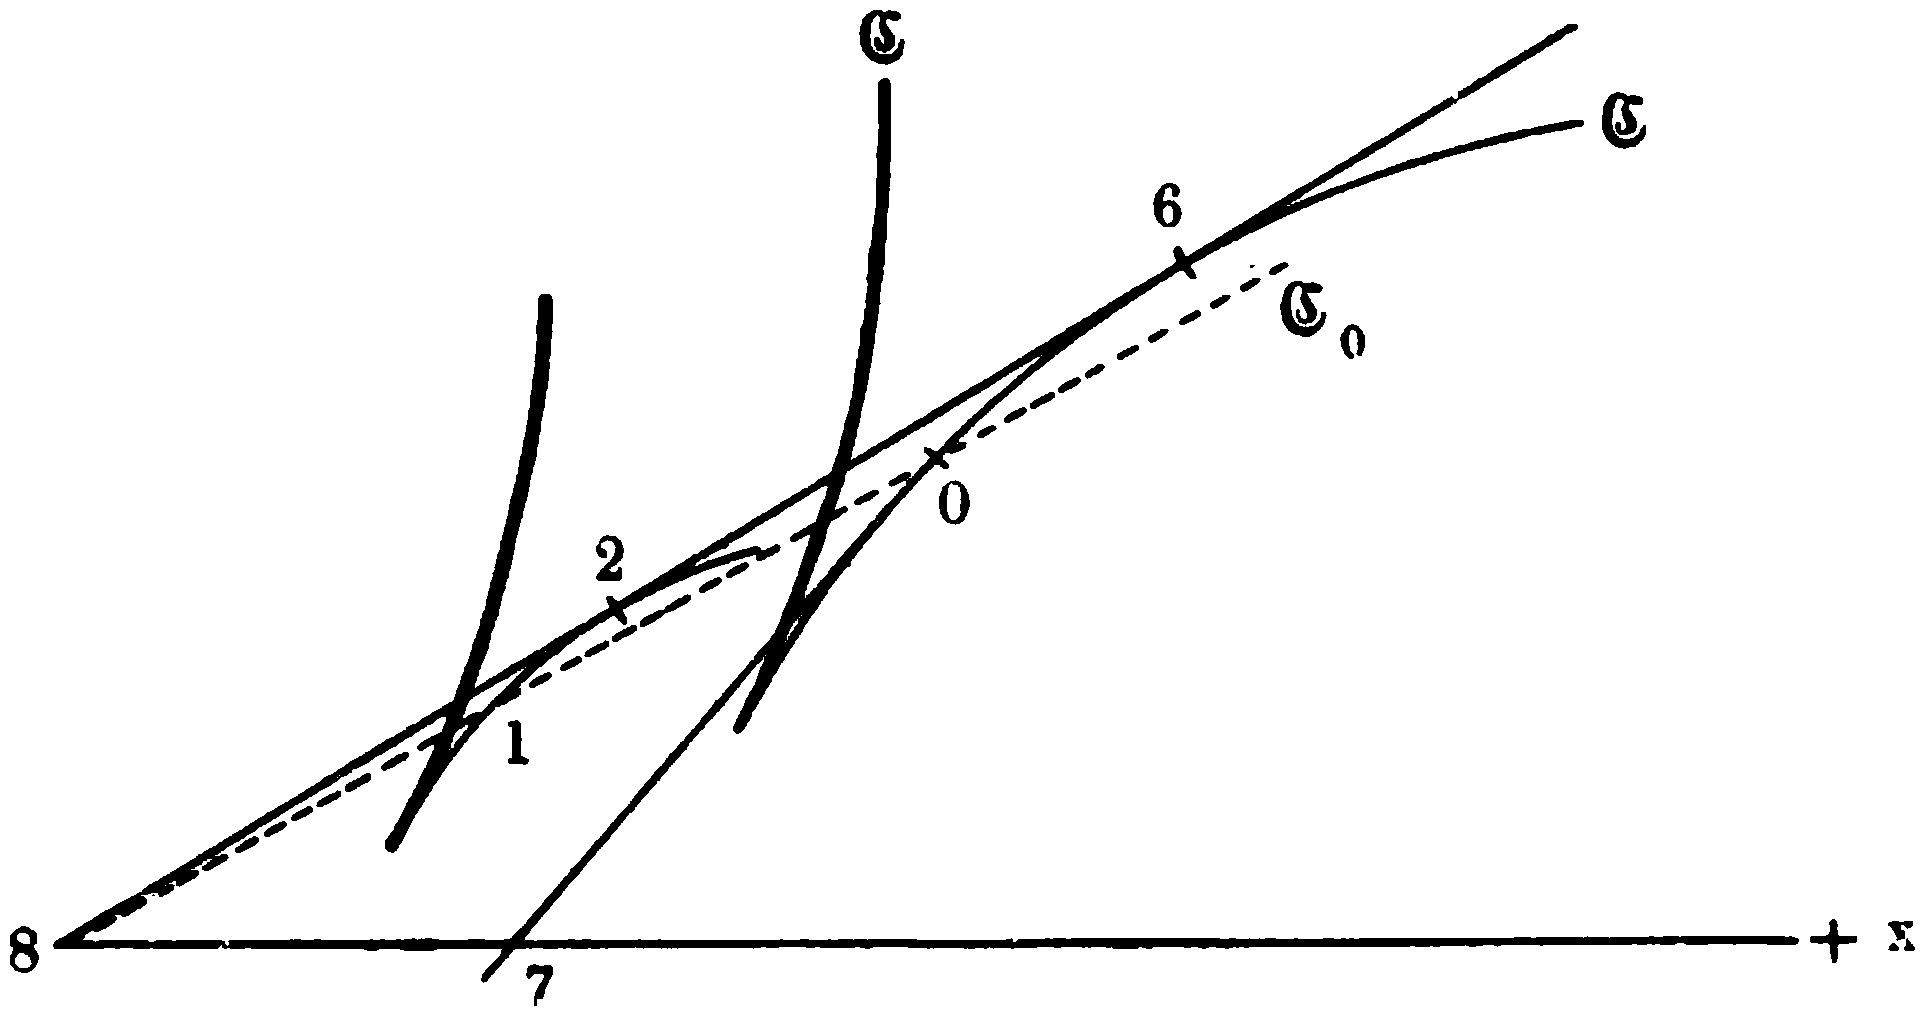
\includegraphics[width=\linewidth,height=36mm,keepaspectratio]{fig_assets/fig14_src_clean_x8.png}
\end{minipage}\hfill
\begin{minipage}[c]{0.49\linewidth}\centering
\end{minipage}
\end{center}

Den Punkt 8 mache man nun zum Centrum einer Schar von Aehnlichkeitstransformationen; dieselben führen die Curve $\mathfrak{C}$
% src-pdfpage=0122 portion=upper
% src-break=0122
in eine Schar von Extremalen über, welche die Gerade $\mathfrak{C}_0$ transversal schneiden, und die Tangente 68 berühren. Letztere vertritt also die Enveloppe $\mathfrak{C}$ der allgemeinen Theorie, 6 ist der Brennpunkt der Geraden $\mathfrak{C}_0$ auf der Curve $\mathfrak{C}$, und $\mathfrak{C}_1$ ist die Strecke 68. Ist 2 irgend ein Punkt dieser Strecke, und schneidet die in ihm berührende Extremale der construirten Schar die Gerade $\mathfrak{C}_0$ im Punkte 1, so gilt für das Widerstandsintegral die Gleichung
\[
\overline{J}_{12}+J_{26}=\overline{J}_{06},
\]
wobei $J_{26}$ längs der Geraden 68 gebildet wird. Lässt man daher den Punkt 5 längs der Curve $\mathfrak{C}$ laufen, so giebt der Bogen 05 ein schwaches Minimum des Widerstandes, verglichen mit den vom Punkte 5 nach der Geraden $\mathfrak{C}_0$ gezogenen Curven, so lange der Punkt 5 dem Bogen 06 angehört; rückt er in die Lage 6 hinein, so zeigt die obige Gleichung, in welcher Weise schon für den Bogen 06 die Minimumseigenschaft verloren geht.

Die bei der Aufgabe VI angewandte Methode zur Construction und Begrenzung eines Feldes kann auf jede Aufgabe übertragen werden, bei welcher die Extremalen einer Schar durch eine bekannte continuirliche Gruppe von Transformationen in einander übergehen. Wo die sogenannten Bahncurven der Transformation die Extremalen der Schar berühren, liegen die Grenzen des Feldes.


% machine-unit: sec27 source=kneser_lvr_1900_archiveorg.pdf#p0122 authorial=true
% src-pdfpage=0122 portion=lower
% src-break=0122
\begin{center}{\large \S~27.}\end{center}

Dass sich die Extremalen wenigstens stückweise mit Feldern umgeben lassen, ist bei den einzelnen Aufgaben meist leicht ersichtlich. Um aber über diese Verhältnisse allgemeine Sätze aufstellen zu können, stellen wir eine functionentheoretische Betrachtung allgemeinen Charakters an, von der auch später noch Gebrauch zu machen sein wird.

In den Differentialgleichungen
\begin{equation}\tag{84}
\frac{dy}{dx}=f(x,y,z,\ldots),\quad
\frac{dz}{dx}=g(x,y,z,\ldots),\ldots,
\end{equation}
deren Anzahl $n$ sei, ebenso wie die Anzahl der Unbekannten $y,z,\ldots$, seien die rechten Seiten regulär in der Umgebung der Stelle
\begin{equation}\tag{85}
x=x_0,\quad y=Y_0,\quad z=Z_0,\ldots;
\end{equation}
% src-pdfpage=0123
% src-break=0123
dann existirt bekanntlich ein Integralsystem, dessen Glieder für $x=x_0$ die willkürlich vorgeschriebenen Werthe
\[
y=y_0,\quad z=z_0,\ldots
\]
annehmen, sobald die Grössen
\[
|y_0-Y_0|,\quad |z_0-Z_0|,\ldots
\]
unterhalb einer gewissen Grenze liegen. Für diese Integrale erhält man Reihen, indem man die Gleichungen (84) nach $x$ differenzirt, und rechts alles durch Functionen von $x,y,z,\ldots$ allein unter Elimination der Differentialquotienten darstellt. Setzt man in den so erhaltenen Ausdrücken, welche ebenfalls in der Stelle (85) regulär sind, für $x,y,z,\ldots$ die Werthe $x_0,y_0,z_0,\ldots$, so erhält man die Coëfficienten der Taylor'schen Entwickelungen jener bestimmten Lösungen $y,z,\ldots$ nach Potenzen von $x-x_0$. Diese Coëfficienten sind, wie in den Beweisen für die Existenz der Integrale gezeigt wird, dem absoluten Betrage nach kleiner als die entsprechenden einer gewissen convergenten Potenzreihe des Arguments $x-x_0$, welche von der speciellen Wahl der Grössen $y_0,z_0,\ldots$ unabhängig ist. Sieht man also letztere als variabel an, so convergiren die für $y,z,\ldots$ erhaltenen Reihen in einem gewissen Gebiete gleichmässig; ihre Werthe für ein bestimmtes Argument $x$ sind also als Potenzreihen von $y_0-Y_0,z_0-Z_0,\ldots$ darstellbar; offenbar kann man setzen
\[
\begin{aligned}
y&=y_0+(x-x_0)[x-x_0,y_0-Y_0,z_0-Z_0,\ldots]_0,\\
z&=z_0+(x-x_0)[x-x_0,y_0-Y_0,z_0-Z_0,\ldots]_0,\ldots,
\end{aligned}
\]
so dass die Functionaldeterminante
\[
\frac{\partial(y,z,\ldots)}{\partial(y_0,z_0,\ldots)}
\]
für $x=x_0$ den Werth $1$ erhält. Die Werthe von $y,z,\ldots$ für irgend ein bestimmtes Argument $x$ sind also als Functionen der Grössen $y_0,z_0,\ldots$ von einander unabhängig.

Nun seien die Grössen $Y,Z,\ldots$ als reguläre, den Gleichungen (84) genügende Functionen von $x$ in einem reellen Intervalle $\mathfrak J$ definirt, welches nach unten durch den Werth $x_0$ begrenzt wird; für diesen sei
\[
Y=Y_0,\quad Z=Z_0,\ldots,
\]
für $x=x_1$ dagegen
\[
Y=Y_1,\quad Z=Z_1,\ldots,
\]
und jedes im Intervalle $\mathfrak J$ erhaltene Werthsystem $(x,Y,Z,\ldots)$ gehöre zu denjenigen, in deren Umgebung die Functionen $f,g,\ldots$
% src-pdfpage=0124
% src-break=0124
regulär sind. Alsdann giebt es der durchgeführten Ueberlegung zufolge positive Grössen $\delta,\varepsilon$ von der Beschaffenheit, dass ein in dem Intervall
\begin{equation}\tag{86}
x_0\leq x\leq x_0+\varepsilon
\end{equation}
reguläres Integralsystem existirt, welches, wenn $x_1$ irgend eine Stelle dieses Intervalls bedeutet, und die Ungleichungen
\[
|y_1-Y_1|<\delta,\quad |z_1-Z_1|<\delta,\ldots
\]
bestehen, für $x=x_1$ die vorgeschriebenen Werthe $y_1,z_1,\ldots$ annimmt. Die Werthe $y,z,\ldots$ an irgend einer bestimmten Stelle des Intervalls (86) sind dann in der Umgebung des Werthsystems $(Y_1,Z_1,\ldots)$ reguläre, von einander unabhängige Functionen von $y_1,z_1,\ldots$. Es sei ferner $\gamma$ die obere Grenze aller möglichen Werthe $\varepsilon$; dann kann die Grösse
\[
\bar x=x_0+\gamma
\]
nicht im Inneren des Intervalls $\mathfrak J$ liegen. Denn wäre dies der Fall, so könnten positive Grössen $\bar\varepsilon,\bar\delta$ so bestimmt werden, dass für das Intervall
\begin{equation}\tag{87}
-\bar\varepsilon<x-\bar x<\bar\varepsilon
\end{equation}
die Grösse $\bar\delta$ dieselbe Bedeutung hätte, wie $\delta$ für das Gebiet (86). Da letzteres aber beliebig nahe an den Punkt $\bar x$ heranreicht, so giebt es in ihm Stellen $x_1$, welche zugleich dem Gebiete (87) angehören; ist daher $\delta_1$ die kleinere der Grössen $\delta,\bar\delta$, und nimmt man an, es sei
\[
|y_1-Y_1|<\delta_1,\quad |z_1-Z_1|<\delta_1,\ldots,
\]
so ist durch jedes diesen Ungleichungen genügende Werthsystem $y_1,z_1,\ldots$ ein Integralsystem definirt, welches in den beiden Gebieten (86), (87), also in dem ganzen Gebiete
\[
x_0\leq x<\bar x+\bar\varepsilon
\]
regulär und so beschaffen ist, dass seine Werthe an einer bestimmten Stelle reguläre, von einander unabhängige Functionen der Grössen $y_1,z_1,\ldots$ sind. Setzte man daher
\[
\varepsilon_1=\gamma+\bar\varepsilon,\quad \bar x+\bar\varepsilon=x_0+\varepsilon_1,
\]
so hätte für das Gebiet
\[
0\leq x-x_0<\varepsilon_1
\]
die Grösse $\delta_1$ dieselbe Bedeutung wie $\delta$ für das Gebiet (86); das widerspräche aber dem Begriffe der oberen Grenze, da $\varepsilon_1>\gamma$. Die obere Grenze aller Werthe $x_0+\varepsilon$ liegt also ausserhalb des
% src-pdfpage=0125 portion=upper
% src-break=0125
Intervalles $\mathfrak J$ oder an der Grenze desselben. Mit dem Intervall (86) kann daher jedes andere identificirt werden, welches von $x_0$ beliebig nahe an die Grenze des Intervalles $\mathfrak J$ heranreicht.

Hiermit ist gezeigt, dass die Integralmannigfaltigkeit $(x,Y,Z,\ldots)$ in folgender Weise mit benachbarten umgeben werden kann. Es giebt Integrale
\[
y=\Phi(x,a,b,\ldots,k),\quad z=\Psi(x,a,b,\ldots,k),\ldots,
\]
welche $n$ Constante $a,b,\ldots,k$ enthalten, und für ein gewisses specielles Werthsystem
\[
a=A,\quad b=B,\ldots,\quad k=K
\]
in die Integrale $Y,Z,\ldots$ übergehen, welche ferner reguläre Functionen ihrer $n+1$ Argumente sind, sobald $x$ dem Inneren des Intervalles $\mathfrak J$ angehört, die Differenzen
\[
|a-A|,\quad |b-B|,\ldots,\quad |k-K|
\]
aber hinreichend klein sind. Unter diesen Voraussetzungen ist die Functionaldeterminante
\[
\frac{\partial(\Phi,\Psi,\ldots)}{\partial(a,b,\ldots)}
\]
von Null verschieden.

% machine-unit: sec28 source=kneser_lvr_1900_archiveorg.pdf#p0125 authorial=true
\begin{center}{\large \S~28.}\end{center}

In dem Integral
\[
J+\Delta J=\int F(x+\delta x,y+\delta y,x'+\delta x',y'+\delta y')\,dt
\]
werde der Integrand nach der Taylor'schen Reihe entwickelt, dann ist das Integral der doppelten Summe aller in den Variationen quadratischen Glieder
\[
\int dt\{F_{xx}\delta x^2+2F_{xy}\delta x\delta y+\cdots+F_{x'x'}\delta x'^2+\cdots\}.
\]
Dieser Ausdruck entsteht aus der Variation
\[
\delta J=\int(F_x\delta x+F_y\delta y+F_{x'}\delta x'+F_{y'}\delta y')\,dt,
\]
indem man die Operation $\delta$ nach den Regeln der Differentiation anwendet und $t,\delta x,\delta x',\delta y,\delta y'$, als dieser Operation gegenüber constant ansieht. Man bezeichnet demgemäss jenen Ausdruck durch $\delta^2J$ und nennt ihn die zweite Variation von $J$. Enthalten die Variationen $\delta x,\delta y$ einen constanten Factor $\varepsilon$, so ist offenbar
\begin{equation}\tag{88}
\Delta J=\delta J+\frac12\delta^2J+[\varepsilon]_3,
\end{equation}
% src-pdfpage=0126
% src-break=0126
und $\delta^2J$ enthält den Factor $\varepsilon^2$. Nun kann man setzen:
\[
\delta J=F_{x'}\delta x+F_{y'}\delta y+
\int dt(P\delta x+Q\delta y),
\]
also folgt, da das Zeichen $\delta$ mit dem der Integration nach $t$ zu vertauschen ist
\[
\delta^2J=\delta F_{x'}\delta x+\delta F_{y'}\delta y+
\int dt(\delta P\delta x+\delta Q\delta y),
\]
eine Formel, die sehr leicht durch Rechnung zu verificiren ist. Speciell in dem Falle
\[
\left.\delta x\right|^0=\left.\delta x\right|^1=
\left.\delta y\right|^0=\left.\delta y\right|^1=0
\]
erhält man
\[
\delta^2J_{01}=\int_0^1dt(\delta P\delta x+
\delta Q\delta y).
\]

Diese Formel werde auf eine Normalvariation angewandt, welche durch die Gleichungen
\[
\delta x=\omega X,
\quad
\delta y=\omega Y
\]
definirt ist, wobei $X,Y$ dieselbe Bedeutung wie in \S~24 haben und $\omega$ an den Stellen 0 und 1 verschwindet. Dann ist nach der dort abgeleiteten Identität (75)
\begin{equation}\tag{89}
\delta^2J_{01}=\int_0^1\omega(X\delta P+Y\delta Q)\,dt
=\int_0^1\omega\left(F_2\omega-\frac{d(F^1\omega')}{dt}\right)dt
\end{equation}
oder nach einer partiellen Integration
\begin{equation}\tag{90}
\delta^2J_{01}=\int_0^1dt\,(F^1\omega'^2+F_2\omega^2).
\end{equation}

Jetzt seien wiederum 0 und 6 conjugirte Punkte; über letzteren reiche der Bogen 02 hinaus. Dann hat nach \S~24 die Gleichung
\begin{equation}\tag{91}
F_2\omega-\frac{d(F^1\omega')}{dt}=0
\end{equation}
ein in den Punkten 0 und 6 verschwindendes Integral, welches im Punkte 6 sein Zeichen ändert; der Bogen 02 sei so begrenzt, dass 0 und 6 die einzigen ihm angehörigen Nullstellen des Integrals $\omega$ sind. Ist dann $\varepsilon$ eine hinreichend kleine Constante und $F^1$ längs des ganzen Bogens 02 von Null verschieden, so hat die Gleichung
\[
(F_2-\varepsilon)w-\frac{d(F^1w')}{dt}=0
\]
nach \S~27 ein Integral, welches wie $\omega$ auf der Strecke 02 regulär ist, der Gleichung
% src-pdfpage=0127
% src-break=0127
\[
\left.w\right|^0=\left.\omega\right|^0=0
\]
genügt, und ebenfalls zwischen 0 und 2 eine einzige Nullstelle 7 besitzt, welche für $\varepsilon=0$ mit 6 zusammenfällt. Dann hat man nach den allgemeinen Formeln (89) bei der Normalvariation
\[
\delta x=Xw\alpha,
\quad
\delta y=Yw\alpha,
\]
in welcher $\alpha$ constant sei, die Formel
\[
\delta^2J_{07}=\alpha^2\int_0^7 w\left(F_2w-\frac{d(F^1w')}{dt}\right)dt
=\alpha^2\varepsilon\int_0^7w^2dt.
\]
Setzt man daher in dem Intervall 72
\[
\delta x=\delta y=0,
\]
so hat man, da der Punkt 7 bei hinreichend kleinem $\varepsilon$ dem Inneren des Intervalls 02 angehört,
\[
\delta^2J_{02}=\delta^2J_{07}=\alpha^2\varepsilon\int_0^7\omega^2dt,
\]
und da die variirte Curve eine Extremale ist, nach (88)
\[
\delta J_{02}=0,
\quad
\Delta J_{02}=\frac12\delta^2J_{07}+[\alpha]_3
=\frac{\alpha^2\varepsilon}{2}\int_0^7w^2dt+[\alpha]_3.
\]
Diese Grösse hat offenbar, sobald $\alpha$ klein genug ist, das Vorzeichen mit $\varepsilon$ gemein, kann also sowohl positiv wie negativ werden, so dass der Bogen 02 sicher kein Extremum des Integrals $J$ liefert.

Diese in ihren Grundgedanken von Erdmann und Weierstrass herrührende Betrachtung unterscheidet sich von den in \S\S~24, 25 gegebenen dadurch, dass letztere im Allgemeinen schon für einen von zwei conjugirten Punkten begrenzten Bogen das Extremum als nicht vorhanden nachweisen, aber einen Ausnahmefall ausschliessen; die soeben durchgeführte Entwickelung erstreckt sich auch auf den Ausnahmefall, verlangt aber stets, dass der betrachtete Bogen über den zu seinem Anfangspunkte conjugirten Punkt hinausreiche.

Falls der Bogen 01 kein Paar conjugirter Punkte enthält, und $F^1$ auf ihm nicht verschwindet, lehrt die Formel (90), dass das Vorzeichen der zweiten Variation mit dem der Grösse $F_1$ oder $F^1$ übereinstimmt. Wenn nämlich $u$ eine von $t_0$ bis $t_1$ reguläre Function von $t$ ist, hat man offenbar
\[
\int_0^1(u'\omega^2+2u\omega\omega')\,dt
=\int_0^1\frac{d}{dt}(u\omega^2)\,dt
=u\omega^2\bigg|_0^1=0,
\]
% src-pdfpage=0128
% src-break=0128
\begin{equation}\tag{92}
\delta^2J_{01}=\int_0^1dt\,[F^1\omega'^2+2u\omega\omega'+(F_2+u')\omega^2],
\end{equation}
und in diesem Ausdruck hat der Integrand dasselbe Vorzeichen wie $F_1$, wenn man $u$ der Gleichung
\begin{equation}\tag{93}
(F_2+u')F^1-u^2=0
\end{equation}
gemäss bestimmen kann; dann hat man einfach
\begin{equation}\tag{94}
\delta^2J_{01}=\int_0^1F^1\left(\omega'+\frac{u\omega}{F^1}\right)^2dt.
\end{equation}
Die Gleichung (93) kann aber wie jede Gleichung von der Form
\[
u'=Lu^2+Mu+N
\]
auf eine lineare Differentialgleichung zweiter Ordnung zurückgeführt werden; indem man setzt:
\[
u=-\frac1L\frac{\omega'}{\omega},
\]
erhält man
\[
\omega''-\left(M+\frac{L'}L\right)\omega'+LN\omega=0;
\]
von der Gleichung (93) aus kommt man auf diese Weise genau zu der Gleichung (91), welcher die Grösse $\Delta(t,a):\sqrt{\xi_t^2+\eta_t^2}$ genügt. Diese ist bei der eingeführten Voraussetzung längs des Bogens 01 von Null verschieden, ergiebt somit eine im Integrationsintervall reguläre Grösse $u$:
\[
u=-\frac{F_1\sqrt{\xi_t^2+\eta_t^2}}{\Delta(t,a)}\frac{d}{dt}\left(\frac{\Delta(t,a)}{\sqrt{\xi_t^2+\eta_t^2}}\right).
\]
Wenn also eine Schar von Extremalen bekannt ist, so kann für einen Bogen von der vorausgesetzten Beschaffenheit und für eine Normalvariation die Formel (94) explicite hergestellt werden.

Einen Beweis für das Eintreten des Extremums gegenüber allen Curven, welche durch eine Normalvariation aus $\mathfrak C$ hervorgehen und einer engeren Nachbarschaft angehören, erhält man, wenn man die Gleichung (93), indem man unter $\varepsilon$ eine hinreichend kleine Constante versteht, durch folgende ersetzt:
\[
(F_2+u')F^1-u^2=\varepsilon^2.
\]
Diese hat nach \S~27, wenn $\varepsilon$ hinreichend klein ist, ebenso wie jene ein von 0 bis 1 reguläres Integral; führt man dasselbe in die Formel (92) ein, so ist die unter dem Integralzeichen stehende quadratische Form definit, und die Formel
% src-pdfpage=0129 portion=upper
% src-break=0129
\[
\Delta J_{01}=\frac12\delta^2J_{01}+\int_0^1[\omega,\omega']_3\,dt
\]
ergiebt leicht, dass das Extremum wirklich eintritt.

% machine-unit: sec29 source=kneser_lvr_1900_archiveorg.pdf#p0129 authorial=true
\begin{center}{\large \S~29.}\end{center}

Ist 02 irgend ein Curvenstück, das in der Umgebung jedes seiner Punkte regulär ist (\S~1), so können längs desselben $x$ und $y$ stets als reguläre eindeutige Functionen eines Parameters $t$ dargestellt werden, z.~B. der von 0 nach 2 hin gemessenen Bogenlänge. Diese wird durch die Gleichungen
\[
\frac{dt}{dx}=\sqrt{1+\left(\frac{dy}{dx}\right)^2},
\quad
\frac{dt}{dy}=\sqrt{1+\left(\frac{dx}{dy}\right)^2}
\]
definirt, in welchen jede der Quadratwurzeln dasselbe Zeichen hat, wie das unter ihr im Nenner stehende Differential beim Fortgang in der Richtung 02. Ist nämlich an der Stelle 1 die Grösse $dy:dx$ endlich, also $y$ eine reguläre Function von $x$, so gilt dasselbe von $\frac{dt}{dx}$, und diese Grösse ist von Null verschieden:
\[
\frac{dt}{dx}=\left.\frac{dt}{dx}\right|^1+[x-x_1]_1,
\quad
t-t_1=\left.\frac{dt}{dx}\right|^1(x-x_1)+[x-x_1]_2;
\]
die zweite Gleichung ergiebt aber
\[
x-x_1=[t-t_1]_1,
\]
so dass $x$ und $y$ an der Stelle 1 reguläre Functionen von $t$ sind. Dasselbe Resultat erhält man natürlich durch eine ähnliche Entwickelung, wenn $dx:dy$ endlich und demnach $x$ als reguläre Function von $y$ darstellbar ist. Die Festsetzung über die Vorzeichen der Quadratwurzeln bewirkt, dass $dt$ beim Fortgang in der Richtung 02 immer positiv ist, so dass zu verschiedenen Werthen von $t$ verschiedene Punkte des Bogens gehören.

Bildet nun der Bogen 02 einen Theil einer Extremale und definirt er nur Werthsysteme $(x,y,x',y')$, in deren Umgebung der Integrand $F$ regulär ist, so gelten die Gleichungen
\[
x'^2+y'^2=1,
\quad
F_1=F^1,
\quad
F_x-F_{x'}'=F_y-F_{y'}'=0,
\]
aus denen wir die beiden gleichbedeutenden Systeme ableiten:
\begin{equation}\tag{95}
\begin{aligned}
F_x-F_{x'x}x'-F_{x'y}y'-F_{x'x'}x''-F_{x'y'}y''&=0,\\
x'x''+y'y''&=0;
\end{aligned}
\end{equation}
% src-pdfpage=0130
% src-break=0130
\begin{equation}\tag{96}
\begin{aligned}
F_y-F_{y'x}x'-F_{y'y}y'-F_{y'x'}x''-F_{y'y'}y''&=0,\\
x'x''+y'y''&=0.
\end{aligned}
\end{equation}
Aus jedem derselben können $x'',y''$ als Functionen von $x,y,x',y'$ berechnet werden, und erscheinen als Brüche, deren Zähler längs des Bogens 02 reguläre Functionen von $t$, und deren Nenner die Determinanten
\[
\begin{vmatrix}
F_{x'x'}&F_{x'y'}\\
x'&y'
\end{vmatrix},
\quad
\begin{vmatrix}
F_{y'x'}&F_{y'y'}\\
x'&y'
\end{vmatrix}
\]
sind, welche mit Berücksichtigung der in \S~16 abgeleiteten Identitäten in folgende Form gebracht werden können:
\[
F_1y'(x'^2+y'^2)=F_1y'=\frac{\bar f_{qq}}{y'^2},
\quad
F_1x'(x'^2+y'^2)=F_1x'=\frac{f_{pp}}{x'^2}.
\]
Führen wir daher die in \S~17 geltende Beschränkung wieder ein, dass für jedes Linienelement des Bogens 02 die Grösse $F_1$ von Null verschieden sei, womit möglicherweise gewisse singuläre Lösungen der Gleichungen (95), (96) ausgeschlossen werden, so erhält man für $x''$ und $y''$, indem man das eine oder andere der Systeme (95), (96) zu Grunde legt, Ausdrücke, die in der Umgebung jedes durch ein Element des Bogens 02 definirten Werthsystems $(x,y,x',y')$ regulär sind. Schreibt man für diese Ausdrücke
\[
\frac{dx'}{dt}=M(x,y,x',y'),
\quad
\frac{dy'}{dt}=N(x,y,x',y')
\]
und fügt die Gleichungen
\[
\frac{dx}{dt}=x',
\quad
\frac{dy}{dt}=y'
\]
hinzu, deren rechte Seiten stets regulär sind, so erhält man ein System von der in \S~27 betrachteten Beschaffenheit, in welchem $x$ durch $t$ ersetzt ist, und das Intervall $\mathfrak J$ von $t_0$ oder 0 bis $t_2$ reicht. Es giebt daher ein Integralsystem von der Form
\begin{equation}\tag{97}
x=X(t,a,b,\alpha,\beta),
\quad
y=Y(t,a,b,\alpha,\beta),
\end{equation}
in welchem die Functionen $X,Y$ regulär sind, sobald $t$ dem bezeichneten Intervall angehört, und die Differenzen
\[
|a-x_0|,
\quad
|b-y_0|,
\quad
|\alpha-x'_0|,
\quad
|\beta-y'_0|
\]
hinreichend klein sind; dabei gelten die Identitäten
\begin{equation}\tag{98}
\begin{aligned}
X(0,a,b,\alpha,\beta)&=a,
&X_t(0,a,b,\alpha,\beta)&=\alpha,\\
Y(0,a,b,\alpha,\beta)&=b,
&Y_t(0,a,b,\alpha,\beta)&=\beta.
\end{aligned}
\end{equation}
Führt man daher die Bedingung
% src-pdfpage=0131 portion=upper
% src-break=0131
\[
\alpha^2+\beta^2=1
\]
ein, so hat man nach der zweiten Gleichung (95) allgemein
\[
X_t^2+Y_t^2=1,
\]
und die Grösse $t$ repräsentirt auch auf allen Curven
\[
x=X,
\quad
y=Y
\]
die Bogenlänge, gemessen vom Punkte $(a,b)$ an.

% machine-unit: sec30 source=kneser_lvr_1900_archiveorg.pdf#p0131 authorial=true
\begin{center}{\large \S~30.}\end{center}

Setzen wir nun die Gleichung
\begin{equation}\tag{99}
\Gamma(a,b)=0
\end{equation}
an, welche, wenn $a$ und $b$ Coordinaten sind, eine in der Stelle $a=x_0,b=y_0$ reguläre Curve $\mathfrak C_0$ darstelle, längs deren $\Gamma_a$ und $\Gamma_b$ nirgends zugleich verschwinden, so definiren die Gleichungen (97) eine Schar von Extremalen, welche von den Punkten der Curve $\mathfrak C_0$ mit dem Werthe $t=0$ ausgehen. Sie schneiden diese Curve transversal, wenn die weitere Annahme
\begin{equation}\tag{100}
\Lambda(a,b,\alpha,\beta)=\Gamma_bF_{x'}(a,b,\alpha,\beta)-\Gamma_aF_{y'}(a,b,\alpha,\beta)=0
\end{equation}
eingeführt wird. Offenbar hat man
\[
\begin{aligned}
\Lambda_{\alpha}
&=\Gamma_bF_{x'x'}(a,b,\alpha,\beta)-\Gamma_aF_{y'x'}(a,b,\alpha,\beta)\\
&=\beta F_1(a,b,\alpha,\beta)(\alpha\Gamma_a+
\beta\Gamma_b),\\
\Lambda_{\beta}
&=-\alpha F_1(a,b,\alpha,\beta)(\alpha\Gamma_a+
\beta\Gamma_b);
\end{aligned}
\]
die Functionaldeterminante
\[
\frac{\partial(\Lambda,\alpha^2+\beta^2)}{\partial(\alpha,\beta)}
=2F_1(a,b,\alpha,\beta)(\alpha\Gamma_a+
\beta\Gamma_b)
\]
ist also von Null verschieden, wenn dies von dem Ausdrucke
\[
\alpha\Gamma_a+\beta\Gamma_b
\]
gilt, mithin auch, wenn die Grösse
\[
x'_0\Gamma_a(x_0,y_0)+y'_0\Gamma_b(x_0,y_0)
\]
nicht verschwindet, d.~h. wenn die Curve $\mathfrak C_0$ im Punkte 0 vom Bogen 02 nicht berührt wird. Das könnte nur eintreten, wenn die Gleichungen
\[
\begin{gathered}
x'_0\Gamma_a(x_0,y_0)+y'_0\Gamma_b(x_0,y_0)=0,\\
F_{y'}(x_0,y_0,x'_0,y'_0)\Gamma_a(x_0,y_0)
-F_{x'}(x_0,\ldots,y'_0)\Gamma_b(x_0,y_0)=0
\end{gathered}
\]
zusammen beständen, woraus die Gleichung
\[
F(x_0,y_0,x'_0,y'_0)=0
\]
folgen würde. Schliessen wir diese wie in \S~15 aus, so ergeben die Gleichungen
% src-pdfpage=0132
% src-break=0132
\begin{equation}\tag{101}
\alpha^2+\beta^2=1,
\quad
\Lambda(a,b,\alpha,\beta)=0,
\end{equation}
für $\alpha$ und $\beta$ reguläre Ausdrücke mit den Argumenten $a,b$. Da ferner die Gleichung (99) eine der Grössen $a,b$ als reguläre Function der anderen definirt, z.~B. $b$ als Function von $a$, wenn die Ungleichung
\[
\Gamma_b(x_0,y_0)\gtrless0
\]
gilt, so erscheinen auf Grund der Gleichungen (99), (100), (101) alle vier in $X$ und $Y$ auftretenden Constanten durch $a$ allein ausgedrückt, so dass die Gleichungen der Extremalenschar die Form
\[
x=X=\xi(t,a),
\quad
y=Y=\eta(t,a)
\]
annehmen, und die Functionen $\xi$ und $\eta$ in der Stelle $(0,x_0)$ regulär sind. Dabei ist offenbar
\[
\xi_t=X_t,
\quad
\xi_a=X_a+X_b\frac{db}{da}+X_{\alpha}\frac{d\alpha}{da}+X_{\beta}\frac{d\beta}{da},
\]
und diese Gleichungen bleiben gültig, wenn man $\xi$ durch $\eta$ und $X$ durch $Y$ ersetzt.

Jetzt bilden wir die Functionaldeterminante
\[
2D=\frac{\partial(X,Y,\alpha^2+\beta^2,\Gamma,\Lambda)}{\partial(t,a,b,\alpha,\beta)}
=
\begin{vmatrix}
X_t&X_a&X_b&X_{\alpha}&X_{\beta}\\
Y_t&Y_a&Y_b&Y_{\alpha}&Y_{\beta}\\
0&0&0&2\alpha&2\beta\\
0&\Gamma_a&\Gamma_b&0&0\\
0&\Lambda_a&\Lambda_b&\Lambda_{\alpha}&\Lambda_{\beta}
\end{vmatrix}
\]
und berücksichtigen, dass den Gleichungen (98) zufolge gesetzt werden kann
\[
X=a+\alpha t+[t]_2,
\quad
Y=b+\beta t+[t]_2;
\]
dann ergiebt sich für $t=0$:
\[
\begin{gathered}
X_a=1,
\quad X_b=X_{\alpha}=X_{\beta}=0,
\quad X_t=\alpha,\\
Y_b=1,
\quad Y_a=Y_{\alpha}=Y_{\beta}=0,
\quad Y_t=\beta,
\end{gathered}
\]
mithin auf Grund der obigen Werthe $\Lambda_{\alpha},\Lambda_{\beta}$:
\[
D\big|_{t=0}=
\begin{vmatrix}
\alpha&1&0&0&0\\
\beta&0&1&0&0\\
0&0&0&\alpha&\beta\\
0&\Gamma_a&\Gamma_b&0&0\\
0&\Lambda_a&\Lambda_b&\beta&-\alpha
\end{vmatrix}
F_1(\alpha\Gamma_a+\beta\Gamma_b)
=-F_1(\alpha\Gamma_a+
\beta\Gamma_b)^2,
\]
% src-pdfpage=0133
% src-break=0133
ein Werth, der offenbar von Null verschieden ist. Multiplicirt man nun in $D$ die dritte, vierte und fünfte Verticalreihe mit
\[
\frac{db}{da},\quad \frac{d\alpha}{da},\quad \frac{d\beta}{da}
\]
und addirt sie zur zweiten, so ergiebt sich:
\[
\begin{aligned}
D
&=
\begin{vmatrix}
\xi_t&\xi_a\\
\eta_t&\eta_a
\end{vmatrix}
\begin{vmatrix}
0&\alpha&\beta\\
\Gamma_b&0&0\\
\Lambda_b&\Lambda_{\alpha}&\Lambda_{\beta}
\end{vmatrix}\\
&=
\begin{vmatrix}
\xi_t&\xi_a\\
\eta_t&\eta_a
\end{vmatrix}
\Gamma_bF_1(\alpha\Gamma_a+\beta\Gamma_b);
\end{aligned}
\]
mithin ist auch die Grösse
\[
\Delta=\frac{\partial(\xi,\eta)}{\partial(t,a)}
\]
in der Nähe der Stelle 0 von Null verschieden. Die construirten Extremalen, welche die Curve $\mathfrak C_0$ transversal schneiden, bilden also, wenn man sie nicht über eine gewisse Grenze hinaus in Betracht zieht, genau im Sinne des \S~14 ein Feld des Bogens 02 oder eines in 0 beginnenden endlichen Theiles desselben.

Die Grösse $D$ enthält, wenn man sie für die Curven 02 bildet, nur die ersten und zweiten Ableitungen von $\Gamma$ für das Werthsystem $a=x_0,b=y_0$; man schliesst daraus leicht, dass irgend zwei Curven $\mathfrak C_0$, welche sich im Punkte 0 osculiren, auf der Extremale 02 dieselben Brennpunkte haben. Zieht sich die Curve $\mathfrak C_0$ in einen Punkt 0 zusammen, so sind $a$ und $b$ nicht mehr frei veränderlich und können unter den Functionszeichen $X,Y$ weggelassen werden. Die Determinante
\[
D_0(t)=
\begin{vmatrix}
X_t&X_{\alpha}&X_{\beta}\\
Y_t&Y_{\alpha}&Y_{\beta}\\
0&\alpha&\beta
\end{vmatrix}
=\frac{\partial(X,Y,\alpha^2+\beta^2)}{\partial(t,\alpha,\beta)}
\]
kann den Gleichungen (98) zufolge geschrieben werden:
\[
D_0(t)=
\begin{vmatrix}
\alpha+[t]_1&t+[t]_2&[t]_2\\
\beta+[t]_1&[t]_2&t+[t]_2\\
0&\alpha&\beta
\end{vmatrix}
=\begin{vmatrix}
\alpha&t&0\\
\beta&0&t\\
0&\alpha&\beta
\end{vmatrix}+[t]_2=-t+[t]_2,
\]
sie verschwindet also zwar im Punkte 0 selbst, nicht aber in der Umgebung desselben. Ist nun z.~B. $y'_0$ von Null verschieden, $\beta$ als Function von $\alpha$ also an der Stelle $x'_0$ regulär, und setzen wir
% src-pdfpage=0134 portion=upper
% src-break=0134
\[
X(t,\alpha,\sqrt{1-\alpha^2})=\xi(t,\alpha),
\quad
Y(t,\alpha,\sqrt{1-\alpha^2})=\eta(t,\alpha),
\]
so sind $\xi$ und $\eta$ an der Stelle $(0,x'_0)$ regulär, und es ist
\[
\alpha+\beta\frac{d\beta}{d\alpha}=0,
\]
\[
\xi_{\alpha}=X_{\alpha}+X_{\beta}\frac{d\beta}{d\alpha},
\quad
\eta_{\alpha}=Y_{\alpha}+Y_{\beta}\frac{d\beta}{d\alpha};
\]
hieraus folgt leicht:
\[
D_0(t)=\frac{\partial(\xi,\eta)}{\partial(t,\alpha)}\beta=\beta\Delta.
\]
Mithin ist auch $\Delta$ in der Umgebung des Punktes 0 von Null verschieden, und wenn 1 ein hinreichend nahe bei 0 liegender Punkt des Bogens 02 ist, kann der Bogen 12 wenigstens in der Nähe des Punktes 1 mit einem Felde umgeben werden, dessen Extremalen alle durch den Punkt 0 gehen.

% machine-unit: sec31 source=kneser_lvr_1900_archiveorg.pdf#p0134 authorial=true
\begin{center}{\large \S~31.}\end{center}

Beschränken wir die vier in $X$ und $Y$ auftretenden Constanten nur durch die Relationen
\[
\alpha^2+\beta^2=1,
\quad
\Gamma(a,b)=0,
\]
so können wir sie durch zwei Constante ausdrücken, etwa $a$ und
\[
c=\frac{\beta}{\alpha},
\]
wenn die Grössen
\[
x'_0,
\quad
\Gamma_b(x_0,y_0)
\]
von Null verschieden sind. Erhalten wir dann
\begin{equation}\tag{102}
x=\xi(t,a,c),
\quad
y=\eta(t,a,c),
\end{equation}
so sind $\xi$ und $\eta$ regulär an der Stelle
\[
t=0,
\quad
a=x_0,
\quad
c=\frac{y'_0}{x'_0},
\]
und haben die Form
\[
\xi(t,a,c)=a+\frac{t}{\sqrt{1+c^2}}+[t]_2,
\]
\[
\eta(t,a,c)=b+\frac{ct}{\sqrt{1+c^2}}+[t]_2,
\]
wobei die Quadratwurzel beide Male dasselbe Vorzeichen hat. Hieraus ergiebt sich für $t=0$
% src-pdfpage=0135
% src-break=0135
\[
\frac{\partial(\xi,\eta)}{\partial(t,a)}=
\begin{vmatrix}
\dfrac{1}{\sqrt{1+c^2}}&1\\[1.2ex]
\dfrac{c}{\sqrt{1+c^2}}&\dfrac{db}{da}
\end{vmatrix}
=\frac{\dfrac{db}{da}-c}{\sqrt{1+c^2}};
\]
dieser Werth ist, wenn die Grösse
\[
\left|c-\frac{y'_0}{x'_0}\right|
\]
hinreichend klein bleibt, von Null verschieden, da die Extremale $\mathfrak C$ und die Curve $\Gamma=0$ nach Voraussetzung sich nicht berühren. Man kann daher die Gesammtheit aller Extremalen, welche von einer bestimmten, etwa $\mathfrak C$, hinreichend wenig verschieden sind, in der Umgebung eines bestimmten, der letzteren angehörigen Punktes 0 in der Form (102) darstellen, wobei, wenn man $\mathfrak C$ selbst für $a=a_0,c=c_0$ erhält und dem Punkte 0 der Parameter $t_{00}$ zugehört, an der Stelle $(t_{00},a_0,c_0)$ die Functionen $\xi,\eta$ regulär sind, und mindestens eine der Grössen
\[
\theta_1(t,a,c)=\frac{\partial(\xi,\eta)}{\partial(t,a)},
\quad
\theta_2(t,a,c)=\frac{\partial(\xi,\eta)}{\partial(t,c)}
\]
von Null verschieden ist. Jedoch brauchen die Functionen $\xi$ und $\eta$ nicht nothwendig die oben angegebene specielle Form zu haben, welche nur als concretes Beispiel die ausgesprochene Behauptung erweist.

Fasst man nun speciell die durch den Punkt 0 gehenden Extremalen ins Auge, so ist für dieselben
\[
x_0=\xi(t_0,a,c),
\quad
y_0=\eta(t_0,a,c);
\]
diese Gleichungen kann man zufolge der für die Grössen $\theta$ geltenden Voraussetzung nach $t_0$ und $a$ oder $t_0$ und $c$ auflösen; hat man etwa
\[
\theta_2(t_{00},a_0,c_0)\gtrless0,
\]
so erhält man für $t_0-t_{00}$ und $c-c_0$ Ausdrücke von der Form $[a-a_0]_1$, und die mit diesen gebildeten Werthe
\[
\xi(t,a,c)=\xi(t,a),
\quad
\eta(t,a,c)=\eta(t,a)
\]
sind an der Stelle
\[
t=t_{00},
\quad
a=a_0
\]
regulär. Da ferner
\[
\xi_t=\xi_t,
\quad
\xi_a=\xi_a+\xi_c\frac{dc}{da},
\quad
\eta_t=\eta_t,
\quad
\eta_a=\eta_a+\eta_c\frac{dc}{da},
\]
\[
\left.(\xi_tdt_0+\xi_ada+\xi_cdc)\right|^0=0,
\quad
\left.(\eta_tdt_0+\eta_ada+\eta_cdc)\right|^0=0,
\]
% src-pdfpage=0136
% src-break=0136
und letztere Gleichungen ergeben
\[
\frac{dc}{da}=-\frac{\theta_1(t_0,a,c)}{\theta_2(t_0,a,c)},
\]
so erhält man
\[
\Delta=\frac{\partial(\xi,\eta)}{\partial(t,a)}
=\theta_1(t,a,c)+\theta_2(t,a,c)\frac{dc}{da}
=\frac{D(t_0,t)}{\theta_2(t_0,a,c)},
\]
wobei gesetzt ist
\[
D(t_0,t)=
\begin{vmatrix}
\theta_1(t,a,c)&\theta_2(t,a,c)\\
\theta_1(t_0,a,c)&\theta_2(t_0,a,c)
\end{vmatrix}
=-D(t,t_0).
\]
Dieser von Weierstrass betrachtete Ausdruck ist auch die Determinante der Coëfficienten von $dt,dt_0,da,dc$ in den Linearformen $dx_0,dy_0,dx,dy$; man verificirt nämlich leicht die Identität
\[
-D(t_0,t)=
\begin{vmatrix}
\xi_t(t)&0&\xi_a(t)&\xi_c(t)\\
\eta_t(t)&0&\eta_a(t)&\eta_c(t)\\
0&\xi_t(t_0)&\xi_a(t_0)&\xi_c(t_0)\\
0&\eta_t(t_0)&\eta_a(t_0)&\eta_c(t_0)
\end{vmatrix}.
\]
Der für $\Delta$ erhaltene Ausdruck zeigt, dass die Jacobi'sche Bedingung des Extremums auf irgend einer Extremale für den Bogen 12 erfüllt ist, wenn die Punkte 0, 1, 2 in der Richtung wachsender $t$ auf einander folgen und die Gleichung
\[
D(t_0,t)=0
\]
in dem Intervall von $t_0$ bis $t_2$ keine andere Wurzel als $t=t_0$ besitzt. Diese Form der Jacobi'schen Bedingung benutzt den ausserhalb des untersuchten Bogens 12 liegenden Punkt 0, ein Uebelstand, dem in folgender Weise abzuhelfen ist. Liegen $t$ und $t_0$ in der Nähe eines festen Werthes $t_1$, so kann man entwickeln
\begin{equation}\tag{103}
\begin{aligned}
D(t,t_0)&=[t-t_1,t_0-t_1]_1\\
&=[(t-t_0)+(t_0-t_1),t_0-t_1]_1
=\sum_a^{1,\infty}f_a(t_0)(t-t_0)^a;
\end{aligned}
\end{equation}
die Coëfficienten dieser Reihe erscheinen zunächst als Functionen von $t_0$ und $t_1$, müssen aber von letzterem Argument ebenso wie $D(t,t_0)$ unabhängig sein. Da ferner $\theta_1$ und $\theta_2$ als specielle Fälle der Grösse $\Delta$ angesehen werden können, welche nach \S~24 nicht mit ihrer Ableitung nach $t$ zugleich verschwindet, so gilt dasselbe von $D(t,t_0)$, wenn dieser Ausdruck nicht identisch verschwindet, und es folgt
% src-pdfpage=0137
% src-break=0137
\[
|f_1(t_0)|>0.
\]
Beschränkt man daher die Grösse $t_0$ auf ein gewisses Intervall
\begin{equation}\tag{104}
|t_0-t_1|<\varepsilon,
\end{equation}
so liegt die Grösse $|f_1(t_0)|$ oberhalb einer positiven Grenze $\gamma$. Der ursprünglichen Entwickelung (103) zu Folge giebt es ferner solche positive Constante $g,\rho$, dass bei der Voraussetzung
\begin{equation}\tag{105}
|t_0-t_1|<\rho,
\quad
|t-t_1|<\rho
\end{equation}
die Ungleichung
\[
\frac1{a!}\left|\frac{\partial^aD(t_0,t)}{\partial t^a}\right|<g\rho^{-a}
\]
besteht, und da die linke Seite für $t=t_0$ in $|f_a(t_0)|$ übergeht, folgt bei Voraussetzung der ersten Ungleichung (105)
\[
|f_a(t_0)|<g\rho^{-a},
\]
\[
\left|\sum_{a=2}^{\infty}f_a(t_0)(t-t_0)^{a-1}\right|
<\frac{g}{\rho}\sum_{a=2}^{\infty}\left|\left(\frac{t-t_0}{\rho}\right)^{a-1}\right|.
\]
Es giebt daher eine nur von $g,\rho,\gamma$, nicht aber von $t_0$ abhängige positive Constante $\delta$ von der Beschaffenheit, dass bei der Annahme
\[
|t-t_0|<\delta
\]
und den Voraussetzungen (104), (105) die Ungleichung
\[
\left|f_1(t_0)+\sum_{a=2}^{\infty}f_a(t_0)(t-t_0)^{a-1}\right|>0
\]
besteht, die Gleichung
\[
D(t_0,t)=0
\]
also zwischen $t_0-\delta$ und $t_0+\delta$ keine andere Wurzel besitzt, als $t=t_0$.

Jetzt werde $t_0$ so nahe bei $t_1$ angenommen, dass nicht nur die Relationen (104), (105) erfüllt sind, sondern auch, wenn $\delta_0$ eine zwischen 0 und $\delta$ liegende Constante ist, die Ungleichungen
\begin{equation}\tag{106}
t_0<t_1<t_0+\delta,
\quad
t_0+\delta>t_1+\delta_0
\end{equation}
bestehen. Vorausgesetzt werde ferner, dass die Gleichung
\begin{equation}\tag{107}
D(t_1,t)=0
\end{equation}
in dem Intervall von $t_1$ bis $t_2$ allein die Wurzel $t=t_1$ habe, in dem Intervall von $t_1+\delta_0$ bis $t_2$ also gar keine. Dann gilt letzteres auch, sobald $|t_1-t_0|$ hinreichend klein ist, für die Gleichung
\[
D(t_0,t)=0,
\]
% src-pdfpage=0138
% src-break=0138
welche zwischen $t_0-\delta$ und $t_0+\delta$, mithin auch nach (106) zwischen $t_0-\delta$ und $t_1+\delta_0$ nur die eine Wurzel $t_0$ besitzt; diese ist also auch die einzige Wurzel der letzten Gleichung für das ganze Intervall von $t_0$ bis $t_2$. Damit ist gezeigt, dass unter der für die Gleichung (107) eingeführten Voraussetzung die Jacobi'sche Bedingung in der oben angegebenen Form erfüllt ist, d.~h. dass die durch einen passend gewählten Punkt 0 gehenden Extremalen ein Feld des Bogens 12 bilden. Die Jacobi'sche Bedingung kann daher auch, wenn es sich um das Extremum für den Bogen 12 bei festen Endpunkten handelt, durch die Forderung ersetzt werden, dass die Gleichung (107) auf der Strecke von $t_1$ bis $t_2$ keine andere Wurzel als $t=t_1$ besitze.

Kann man speciell $x=t$ setzen, so erhält man
\[
y=\eta(x,a,c),
\quad
\theta_1=\frac{\partial y}{\partial a},
\quad
\theta_2=\frac{\partial y}{\partial c},
\]
\[
D(t_0,t)=\Delta(x_0,x)=
\begin{vmatrix}
\dfrac{\partial y}{\partial a}&\dfrac{\partial y}{\partial c}\\[1.2ex]
\left.\dfrac{\partial y}{\partial a}\right|^0&
\left.\dfrac{\partial y}{\partial c}\right|^0
\end{vmatrix};
\]
setzt man diesen Ausdruck gleich Null, so hat man das Kriterium der conjugirten Punkte in der von Hesse gegebenen Form.



% src-pdfpage=0139
% src-break=0139
\begin{center}
{\large Vierter Abschnitt.}\par
\vspace{4mm}
{\Large\bfseries Das einfachste relative Extremum.}\par
\vspace{2mm}\rule{26mm}{0.4pt}\par
\end{center}

\begin{center}{\large \S~32.}\end{center}

Die isoperimetrische Aufgabe im weiteren Sinne des Wortes verlangt, ein Integral
\[
J=\int f(x,y,p)\,dx=\int F(x,y,x',y')\,dt
\]
zu einem Extremum zu machen, wenn ein anderes Integral derselben Form
\[
K=\int g(x,y,p)\,dx=\int G(x,y,x',y')\,dt
\]
einen vorgeschriebenen Werth hat; d.~h. unter allen Curven, welche dem Integral $K$ den vorgeschriebenen Werth geben, diejenige zu finden, längs deren $J$ einen extremen Werth erhält. Ein solches Extremum heisst ein \textbf{relatives}, die bisher betrachteten im Gegensatz dazu \textbf{absolute} Extrema. Die isoperimetrische Aufgabe im engeren Sinne erhält man, wenn $J$ das Flächenintegral und $K$ die Bogenlänge ist.

Um nun zunächst nothwendige Bedingungen dieses Extremums abzuleiten, sei $\mathfrak{B}$ ein Curvenstück von den in \S\S~2 und 4 für den ebenso bezeichneten Bogen geforderten Eigenschaften; die Functionen $F$ und $G$ seien regulär für die durch die Elemente dieses Bogens definirten Argumentsysteme. Längs desselben mögen die Punkte 0, 1, 2, 3 in der Richtung wachsender Werthe von $t$ auf einander folgen; dann variiren wir die beiden Bögen 01 und 23 nach der in \S~8 benutzten Methode.

Bezeichnen wir durch $\varepsilon,\eta,\bar\varepsilon,\bar\eta$ Constante, und setzen
\[
T=(t-t_0)^3(t_1-t)^3,
\quad
U=(t-t_2)^3(t_3-t)^3,
\]
so sei für den Bogen 01
% src-pdfpage=0140
% src-break=0140
\[
\delta x=\varepsilon T,
\quad
\delta y=\eta T,
\]
ferner für den Bogen 23
\[
\delta x=\bar\varepsilon U,
\quad
\delta y=\bar\eta U,
\]
ausserhalb der Strecken 01 und 23 aber überall
\[
\delta x=\delta y=0.
\]
Da die ersten und zweiten Ableitungen der Grössen $\delta x,\delta y$ in den Stellen 0, 1, 2, 3 verschwinden, so beschreibt der Punkt $(x+\delta x,y+\delta y)$ eine Curve von den für $\mathfrak{B}$ vorausgesetzten Stetigkeitseigenschaften. Offenbar bestehen in der Bezeichnung der beiden ersten Abschnitte die Gleichungen
\begin{equation}\tag{1}
\Delta J=\Delta J_{01}+\Delta J_{23},
\quad
\Delta K=\Delta K_{01}+\Delta K_{23};
\end{equation}
damit also längs der variirten Curve das Integral $K$ denselben Werth habe, wie längs der ursprünglichen, hat man die Gleichung
\[
\Delta K=\Delta K_{01}+\Delta K_{23}=0
\]
zu erfüllen.

Setzen wir weiter
\[
P=F_x-F'_{x'},\quad Q=F_y-F'_{y'},\quad
R=G_x-G'_{x'},\quad S=G_y-G'_{y'},
\]
so ist nach \S~4, wenn die Variationen an den Grenzen der Integration verschwinden,
\[
\Delta J=\delta J+\int dt\,[\delta x,\delta y,\delta x',\delta y']_2,
\]
\[
\delta J=\int dt\,(P\delta x+Q\delta y),
\]
und analoge Formeln gelten für das Integral $K$; hieraus ergiebt sich bei der angegebenen speciellen Variation auf Grund der Formeln (1)
\[
\begin{aligned}
\Delta J={}&\varepsilon\int_0^1PT\,dt+
\eta\int_0^1QT\,dt+
\bar\varepsilon\int_2^3PU\,dt+
\bar\eta\int_2^3QU\,dt\\
&+[\varepsilon,\eta,\bar\varepsilon,\bar\eta]_2,
\end{aligned}
\]
\[
\begin{aligned}
\Delta K={}&\varepsilon\int_0^1RT\,dt+
\eta\int_0^1ST\,dt+
\bar\varepsilon\int_2^3RU\,dt+
\bar\eta\int_2^3SU\,dt\\
&+[\varepsilon,\eta,\bar\varepsilon,\bar\eta]_2.
\end{aligned}
\]
Soll nun die Curve $\mathfrak{B}$ ein relatives Extremum des Integrals $J$ im definirten Sinne liefern, so muss $\Delta J$ bei allen variirten Curven, für welche $\Delta K$ verschwindet, ein festes Vorzeichen haben. Hieraus folgt, da die Constanten $\varepsilon,\eta,\bar\varepsilon,\bar\eta$ frei verfügbar sind, nach \S~7, dass die Determinanten zweiter Ordnung, welche aus irgend zwei Verticalreihen des Schemas
% src-pdfpage=0141
% src-break=0141
\[
\begin{array}{cccc}
\displaystyle \int_0^1RT\,dt,&\displaystyle \int_0^1ST\,dt,&\displaystyle \int_2^3RU\,dt,&\displaystyle \int_2^3SU\,dt,\\[2.2ex]
\displaystyle \int_0^1PT\,dt,&\displaystyle \int_0^1QT\,dt,&\displaystyle \int_2^3PU\,dt,&\displaystyle \int_2^3QU\,dt,
\end{array}
\]
gebildet sind, verschwinden müssen. Da die Grösse $T$ auf der Strecke 01; ebenso $U$ auf der Strecke 23 positiv ist, kann man dieses Schema in folgende Form bringen:
\[
\begin{array}{cccc}
\displaystyle R_m\int_0^1T\,dt,&\displaystyle S_m\int_0^1T\,dt,&\displaystyle R_\mu\int_2^3U\,dt,&\displaystyle S_\mu\int_2^3U\,dt,\\[2.2ex]
\displaystyle P_m\int_0^1T\,dt,&\displaystyle Q_m\int_0^1T\,dt,&\displaystyle P_\mu\int_2^3U\,dt,&\displaystyle Q_\mu\int_2^3U\,dt,
\end{array}
\]
wobei das Suffix $m$ bedeute, dass für $t$ ein Werth des Intervalls von $t_0$ bis $t_1$ genommen werden soll, und $\mu$ dieselbe Bedeutung für das Intervall von $t_2$ bis $t_3$ hat. Die hier auftretenden Integrale sind alle positiv; es verschwinden also auch alle Determinanten zweiter Ordnung, welche aus Verticalen des Systems
\begin{equation}\tag{2}
\begin{array}{cccc}
R_m,&S_m,&R_\mu,&S_\mu,\\
P_m,&Q_m,&P_\mu,&Q_\mu,
\end{array}
\end{equation}
gebildet sind.

Jetzt bedenken wir, dass $P,Q,R,S$ bei den vorausgesetzten Eigenschaften des Bogens $\mathfrak{B}$ stetige Functionen von $t$ sind; werden also die Strecken 01 und 23, indem man die Punkte 0 und 2 festhält, unbegrenzt verkleinert, so nähern sich die Grössen mit den Suffixen $m$ und $\mu$ bestimmten Grenzwerthen:
\[
\lim P_m=P_0,
\quad
\lim Q_m=Q_0,
\quad
\lim P_\mu=P_2,
\quad
\lim Q_\mu=Q_2,
\]
\[
\lim R_m=R_0,
\quad
\lim S_m=S_0,
\quad
\lim R_\mu=R_2,
\quad
\lim S_\mu=S_2,
\]
und es gilt für die aus diesen Grössen gebildeten Determinanten zweiter Ordnung dasselbe, wie betreffs der Grössen (2). Speciell bestehen die Gleichungen
\[
P_0S_2-R_0Q_2=0,
\quad
Q_0S_2-S_0Q_2=0.
\]
Wir führen nunmehr die Voraussetzung ein, dass die Curve $\mathfrak{B}$ nicht Extremale eines der beiden Integrale $J$ und $K$ sei, so dass weder die Grössen $R$ und $S$, noch die Grössen $P$ und $Q$ längs derselben überall verschwinden. Dann kann man den Punkt 2 so wählen, dass eine der Grössen $P_2,Q_2$, etwa $Q_2$, von Null verschieden ist, und die letzten Gleichungen ergeben
% src-pdfpage=0142
% src-break=0142
\[
P_0\frac{S_2}{Q_2}-R_0=Q_0\frac{S_2}{Q_2}-S_0=0.
\]
Wäre $S_2=0$, so würde aus diesen Gleichungen bei willkürlicher Lage des Punktes 0 folgen
\[
R_0=S_0=0,
\]
die Curve $\mathfrak{B}$ wäre also, entgegen der Voraussetzung, Extremale des Integrals $K$. Es giebt daher eine endliche, von Null verschiedene und von der Lage des Punktes 0 unabhängige Grösse
\[
\lambda=-\frac{Q_2}{S_2}
\]
von der Beschaffenheit, dass die Gleichungen
\[
P_0+\lambda R_0=Q_0+\lambda S_0=0
\]
bestehen. Dieselbe Folgerung ergiebt sich, wenn $P_2$ nicht verschwindet, aus den Gleichungen
\[
P_0R_2-R_0P_2=0,
\quad
Q_0R_2-S_0P_2=0.
\]
Die Curve $\mathfrak{B}$ genügt daher den Differentialgleichungen
\[
F_x-F'_{x'}+\lambda(G_x-G'_{x'})=0,
\quad
F_y-F'_{y'}+\lambda(G_y-G'_{y'})=0,
\]
oder bei der Bezeichnung
\[
H=F+\lambda G
\]
den Gleichungen
\[
H_x-H'_{x'}=0,
\quad
H_y-H'_{y'}=0,
\]
in welchen $\lambda$ eine endliche, von Null verschiedene Constante bedeutet. Jede Curve, welche bei willkürlichem, nicht verschwindendem Werth von $\lambda$ diesen Gleichungen genügt, nennen wir eine Extremale für das vorgelegte Problem des relativen Extremums; da man die Gleichungen durch $\lambda$ dividiren kann, ist ersichtlich, dass die Gesammtheit der Extremalen dieselbe bleibt, wenn die Integrale $J$ und $K$ ihre Rollen vertauschen.

Das Resultat der Untersuchung kann jetzt dahin ausgesprochen werden, dass die Curve, welche das gesuchte relative Extremum liefert, bei den vorausgesetzten Stetigkeitseigenschaften nichts anderes sein kann, als ein Stück einer Extremale, wenn sie nicht etwa für eines der Integrale $J,K$ im Sinne des absoluten Extremums eine Extremale ist. Letzteren Ausnahmefall lassen wir in der allgemeinen Theorie beiseite.

% src-pdfpage=0143
% src-break=0143
\begin{center}{\large \S~33.}\end{center}

Das Integral $J$ sei speciell durch eine Curve 01 zu einem Extremum zu machen, deren Endpunkte nicht gegeben, sondern nur insofern beschränkt sind, als zwischen den Coordinaten $x_0,y_0,x_1,y_1$ irgend welche Relationen
\[
g_b(x_0,y_0,x_1,y_1)=0
\]
vorgeschrieben werden, deren Anzahl nicht grösser als vier sein kann. Eine diese Aufgabe lösende Curve 01 von den Eigenschaften des Bogens $\mathfrak{B}$, die wir als vorhanden annehmen, muss zunächst, abgesehen von dem am Schluss des \S~32 bezeichneten Ausnahmefall, ein Stück einer Extremale sein; denn sonst könnte man sie nach \S~32, ohne ihre Endpunkte zu verschieben, so variiren, dass $J$ bei ungeändertem Werth von $K$ sowohl zu- wie abnähme. Sollen sodann auch die Endpunkte variirt werden, so müssen die Gleichungen
\begin{equation}\tag{3}
g_b(x_0+\delta x_0,\ldots,y_1+\delta y_1)=0
\end{equation}
bestehen. Speciell setzen wir längs eines Bogens 02 der Curve 01
\[
\delta x=\delta x_0\left(\frac{t-t_2}{t_0-t_2}\right)^3,
\quad
\delta y=\delta y_0\left(\frac{t-t_2}{t_0-t_2}\right)^3
+\varepsilon(t_2-t)^3(t-t_0)^3,
\]
und längs eines von diesem getrennten Bogens 31
\[
\delta x=\delta x_1\left(\frac{t-t_3}{t_1-t_3}\right)^3,
\quad
\delta y=\delta y_1\left(\frac{t-t_3}{t_1-t_3}\right)^3,
\]
in dem Mittelstück 23 aber
\[
\delta x=\delta y=0.
\]
Dann sind die Variationen längs der ganzen Curve 01 nebst ihren ersten beiden Ableitungen stetige Functionen von $t$.

Nun hat man allgemein
\[
\Delta K_{01}=G_{x'}\delta x+G_{y'}\delta y\bigg|_0^1+
\int_0^1dt\{R\delta x+S\delta y\}
+[\delta x,\delta y,\delta x',\delta y']_2,
\]
also bei der angegebenen speciellen Variation
\[
\Delta K_{01}=[\delta x_0,\delta y_0,\delta x_1,\delta y_1]_1+
\varepsilon\int_0^2S(t_2-t)^3(t-t_0)^3\,dt
+[\varepsilon,\delta x_0,\delta y_0,\delta x_1,\delta y_1]_2.
\]
% src-pdfpage=0144
% src-break=0144
Hier ist der Factor von $\varepsilon$ von Null verschieden, da 01 eine reguläre Curve ist, auf welcher die Grösse $S$ nur getrennte Nullstellen hat, wenn sie nicht überall verschwindet; in letzterem Falle kann, da die betrachtete Curve nicht Extremale des Integrals $K$ sein soll, die Grösse $R$ nicht längs der Curve 01 überall verschwinden, und man braucht nur in der ganzen Argumentation $x$ und $y$ zu vertauschen. Ist daher $S$ wenigstens stellenweise von Null verschieden, so kann man das Intervall 02 so wählen, dass $S$ in seinem Innern von Null verschieden bleibt. Alsdann kann man aus der Gleichung
\begin{equation}\tag{4}
\Delta K_{01}=0
\end{equation}
ausrechnen
\[
\varepsilon=[\delta x_0,\delta y_0,\delta x_1,\delta y_1]_1.
\]
Andererseits hat man unter der Voraussetzung (4)
\[
\Delta J_{01}=\Delta(J_{01}+\lambda K_{01});
\]
analog der Formel für $\Delta K_{01}$ ergiebt sich hieraus, wenn man die Gleichungen der Extremalen berücksichtigt,
\[
\Delta J_{01}=H_{x'}\delta x+H_{y'}\delta y\bigg|_0^1+
\int_0^1dt\,[\delta x,\delta y,\delta x',\delta y']_2.
\]
Bei der definirten speciellen Variation hat man also, indem man den obigen Ausdruck für $\varepsilon$ einsetzt,
\[
\Delta J_{01}=H_{x'}\delta x+H_{y'}\delta y\bigg|_0^1+
[\delta x_0,\delta y_0,\delta x_1,\delta y_1]_2.
\]
Diese Grösse muss, wenn das gesuchte Extremum durch die Curve 01 geliefert werden soll, bei allen den Gleichungen (3) genügenden Werthen $\delta x_0,\ldots,\delta y_1$ ein festes Vorzeichen haben; das erfordert nach \S~7, dass die Gleichung
\[
H_{x'}\delta x+H_{y'}\delta y\bigg|_0^1=0
\]
eine Folge der linearen Relationen
\[
\frac{\partial g_b}{\partial x_0}\delta x_0+
\frac{\partial g_b}{\partial y_0}\delta y_0+
\frac{\partial g_b}{\partial x_1}\delta x_1+
\frac{\partial g_b}{\partial y_1}\delta y_1=0
\]
sei. Sind speciell $x_0,y_0$ gegeben, und soll der Punkt 1 auf der Curve
\[
h(x,y)=0
\]
liegen, so dass immer
\[
\delta x_0=\delta y_0=0,
\]
so muss die Gleichung
% src-pdfpage=0145
% src-break=0145
\[
H_{x'}\delta x+H_{y'}\delta y\bigg|^1=0
\]
unter der Voraussetzung
\[
h_x\delta x+h_y\delta y\bigg|^1=0
\]
bestehen. Alsdann sagen wir, die Extremale 01 schneide die Curve $h=0$ \textbf{transversal}. Dass dies eintritt, ist eine nothwendige Bedingung dafür, dass die Extremale 01 unter allen vom Punkte 0 zur Curve $h=0$ gezogenen Linien, welche den vorgeschriebenen Werth $K_{01}$ ergeben, ein Extremum des Integrals $J$ liefere.

\begin{center}{\large \S~34.}\end{center}

\noindent\textbf{Beispiele. Aufgabe IX.} Die Curve gegebener Länge zu finden, welche das Flächenintegral zum Maximum macht.

Man hat (\S~4) offenbar mit positiver Quadratwurzel
\[
J=\int y\,dx=\int yx'\,dt,
\quad
K=\int dt\sqrt{x'^2+y'^2},
\]
\[
H=yx'+\lambda\sqrt{x'^2+y'^2},
\quad
H_x=0,
\]
also ergiebt sich als Gleichung der Extremalen zunächst
\begin{equation}\tag{5}
H_{x'}=y+\frac{\lambda x'}{\sqrt{x'^2+y'^2}}=a,
\quad
\frac{dx}{dy}=\frac{a-y}{\lambda\sqrt{1-\left(\dfrac{a-y}{\lambda}\right)^2}},
\end{equation}
und hieraus durch Integration
\[
\frac{x-b}{\lambda}=\sqrt{1-\left(\frac{a-y}{\lambda}\right)^2},
\quad
(y-a)^2+(x-b)^2=\lambda^2.
\]
Die Gesammtheit aller Extremalen ist also mit der aller Kreise der Ebene identisch, und das Quadrat der isoperimetrischen Constante ist dem des Radius gleich. Sind die Endpunkte 0, 1 vorgeschrieben, so ist das Integral $J$ gleich dem Flächenraum zwischen der Curve 01 und der geraden Strecke 01, vermehrt um die constante Fläche des von den Ordinaten der geraden Strecke bestrichenen Trapezes; soll also die erstere Fläche ein Maximum werden, so kann die gesuchte Curve mit den Eigenschaften des Bogens $\mathfrak{C}$ nichts anderes als ein Kreisbogen sein. Die transversale Lage wird durch die Gleichung
\[
H_{x'}Dx+H_{y'}Dy=
\left(y+\frac{\lambda x'}{\sqrt{x'^2+y'^2}}\right)Dx+
\frac{\lambda y'}{\sqrt{x'^2+y'^2}}Dy=0
\]
definirt; an der $x$-Axe ($y=0$) geht sie in die speciellere Form
% src-pdfpage=0146
% src-break=0146
\[
x'Dx+y'Dy=0
\]
über. Soll also die gesuchte Curve in dem gegebenen Punkte 0 beginnen und in einem nicht vorgeschriebenen Punkte der $x$-Axe endigen, so ist die von dieser Axe, der Ordinate des Punktes 0 und der gesuchten Curve begrenzte Fläche bei gegebener Länge der letzteren in keinem anderen Falle ein Maximum, als wenn die Curve ein Kreisbogen ist, dessen Mittelpunkt auf der $x$-Axe liegt. (Vergl. Aufgabe III.)

Ist die gesuchte Curve geschlossen, so stellt das Integral $J$ nach \S~4 den von ihr umschlossenen Flächenraum dar, wenn man längs der Curve genau einmal herum integrirt; man hat dann die Bedingungen
\[
x_0-x_1=y_0-y_1=0,
\quad
\delta x_0-\delta x_1=\delta y_0-\delta y_1=0,
\]
infolge deren die Bedingung
\[
H_{x'}\delta x+H_{y'}\delta y\bigg|_0^1=0
\]
von selbst erfüllt ist, wenn die Curve in ihrem ganzen Verlaufe die Eigenschaften des Bogens $\mathfrak{B}$ hat. Unter dieser Voraussetzung kann sie also bei gegebener Länge einen extremen Inhalt nur dann ergeben, wenn sie ein Kreis ist.

Soll der Inhalt nicht die von der Ordinate bestrichene, sondern die von der gesuchten und einer gegebenen Curve $\mathfrak{H}$
\[
y=h(x)
\]
umschlossene Fläche sein, so hat man
\[
J=\int [y-h(x)]x'\,dt
\]
zu setzen; es wird dann
\[
H=[y-h(x)]x'+\lambda\sqrt{x'^2+y'^2},
\]
die Grössen $H_y,H_{y'}$ und $H_x-H'_{x'}$ sind also dieselben wie im vorigen Falle, so dass die Extremalen auch jetzt noch Kreise sind. Die Bedingung des transversalen Schnittes ist
\[
\left[y-h(x)+\frac{\lambda x'}{\sqrt{x'^2+y'^2}}\right]Dx+
\frac{\lambda y'}{\sqrt{x'^2+y'^2}}Dy=0;
\]
die Curve $\mathfrak{H}$ steht also auf den sie transversal schneidenden Extremalen senkrecht. Geometrisch am interessantesten wird diese Aufgabe, wenn der Endpunkt 1 oder auch beide Endpunkte 0 und 1 nicht vorgeschriebene Punkte der Curve $\mathfrak{H}$ sind; dann
% src-pdfpage=0147
% src-break=0147
ist die Lösung, wenn eine solche existirt, ein zur Curve $\mathfrak{H}$ in einem oder zwei Punkten normaler Kreis.

Das Vorzeichen der Grösse $\lambda$ bestimmt die erste Gleichung (5). Ist nämlich die Richtung wachsender $t$ gegen den nach aussen gehenden Radius des Kreises ebenso gelegen, wie die $+y$- zur $+x$-Axe, so hat man, da $|\lambda|$ stets der Radius des Kreises ist,
\[
\frac{x'}{\sqrt{x'^2+y'^2}}=-\frac{y-a}{|\lambda|},
\]
also $\lambda=|\lambda|$; das entgegengesetzte ergiebt sich, wenn die Richtung wachsender $t$ zum Radius so liegt, wie die $+x$-Axe zur $+y$-Axe.

\medskip
\noindent\textbf{Aufgabe X.} Auf einer gegebenen Fläche eine möglichst kurze Linie zu ziehen, die mit einer gegebenen Curve oder auch, wenn sie geschlossen ist, für sich allein ein Stück von gegebenem Flächeninhalt umschliesst (Curven kürzesten Umrings).

Auf der Fläche seien $x$ und $y$ isometrische, krummlinige Coordinaten, d.~h. die Lage eines Punktes sei durch diese Grössen in einem gewissen, den Punkt $x=y=0$ enthaltenden Gebiet eindeutig bestimmt; dabei habe das Linienelement die Form
\[
ds=\sqrt{M(dx^2+dy^2)}.
\]
Die Ordinate eines Punktes $(x,y)$ nennen wir das von ihm bis zur Linie $y=0$ gezogene Stück einer Linie $x=\mathrm{const}$. Dann ist $Mdx\,dy$ die Grösse eines viereckigen Flächenelements, dessen Seiten Elemente der Linien $x=\mathrm{const}.$ und $y=\mathrm{const}.$ sind. Ist daher
\[
y=h(x)
\]
die Gleichung irgend einer Curve, so ist die von zwei benachbarten Ordinaten derselben begrenzte Fläche
\[
dx\cdot\int_0^ydy\,M=dx\,[N(x,y)-N(x,0)],
\]
wobei $N$ eine der Gleichung
\[
\frac{\partial N}{\partial y}=M
\]
genügende Function von $x$ und $y$ ist. Die Gesammtfläche, welche von den Ordinaten der Curve $y=h(x)$ bedeckt wird, wenn man den Bogen 01 ins Auge fasst, ist demnach
% src-pdfpage=0148
% src-break=0148
\[
\int_0^1dx\{N[x,h(x)]-N[x,0]\}.
\]
Bedeutet sodann $(x,y)$ einen Punkt einer anderen Curve 01, so ist die zwischen beiden liegende Fläche
\[
K=\int_0^1dx\{N[x,y]-N[x,h(x)]\};
\]
das zum Minimum zu machende Integral ist
\[
J=\int_0^1dx\sqrt{M(1+p^2)};
\]
man hat also
\[
H=\sqrt{M(x'^2+y'^2)}+\lambda\{N[x,y]-N[x,h(x)]\}x',
\]
und die eine Gleichung der Extremalen ist
\[
H_y-H'_{y'}=\frac{M_y\sqrt{x'^2+y'^2}}{2\sqrt{M}}+
\lambda Mx'-\frac{d}{dt}\left(\frac{y'\sqrt{M}}{\sqrt{x'^2+y'^2}}\right)=0,
\]
oder, indem man den Winkel $\theta$ durch die Gleichungen
\[
\cos\theta=\frac{x'}{\sqrt{x'^2+y'^2}},
\quad
\sin\theta=\frac{y'}{\sqrt{x'^2+y'^2}}
\]
definirt,
\[
\lambda Mdx=d(\sqrt{M}\sin\theta)-\frac{ds}{\sqrt{M}}\frac{\partial\sqrt{M}}{\partial y}.
\]
Nun ist offenbar
\[
\frac{ds}{\sqrt{M}}=\sqrt{dx^2+dy^2}=dx\cos\theta+dy\sin\theta;
\]
somit ergiebt die vorletzte Gleichung
\[
\begin{aligned}
\lambda Mdx={}&\left(\frac{\partial\sqrt{M}}{\partial x}dx+\frac{\partial\sqrt{M}}{\partial y}dy\right)\sin\theta
+\sqrt{M}\,d\sin\theta\\
&-\frac{\partial\sqrt{M}}{\partial y}(dx\cos\theta+dy\sin\theta)\\
={}&\left(\frac{\partial\sqrt{M}}{\partial x}\sin\theta-\frac{\partial\sqrt{M}}{\partial y}\cos\theta\right)dx+
\sqrt{M}\cos\theta\,d\theta,
\end{aligned}
\]
und da ferner
\[
\cos\theta=\sqrt{M}\frac{dx}{ds},
\quad
\sin\theta=\sqrt{M}\frac{dy}{ds},
\]
so erhält man
% src-pdfpage=0149
% src-break=0149
\[
\lambda M=\frac{\partial\sqrt{M}}{\partial x}\sin\theta-
\frac{\partial\sqrt{M}}{\partial y}\cos\theta+M\frac{d\theta}{ds}.
\]
Betrachtet man nun irgend eine Schar von Extremalen, welche zu demselben Werth von $\lambda$ gehören und einen Theil der Fläche einfach bedecken, so kann $\theta$ als Function von $x$ und $y$ angesehen werden, und man hat
\[
\begin{aligned}
\frac{d\theta}{ds}&=\frac{\partial\theta}{\partial x}\frac{dx}{ds}+
\frac{\partial\theta}{\partial y}\frac{dy}{ds}
=\frac{1}{\sqrt{M}}\left(\cos\theta\frac{\partial\theta}{\partial x}+
\sin\theta\frac{\partial\theta}{\partial y}\right)\\
&=\frac{1}{\sqrt{M}}\left(-\frac{\partial\cos\theta}{\partial y}+
\frac{\partial\sin\theta}{\partial x}\right);
\end{aligned}
\]
diesen Werth in die vorige Gleichung eingesetzt, erhält man
\[
\lambda M=-\frac{\partial(\sqrt{M}\cos\theta)}{\partial y}+
\frac{\partial(\sqrt{M}\sin\theta)}{\partial x}.
\]
Hieraus ist auf Grund einer allgemeinen Formel von \textsc{Bonnet} ersichtlich, dass $\lambda$ die geodätische Krümmung der betrachteten Curve ist. Die Curven kürzesten Umrings haben also constante geodätische Krümmung. Die transversale Lage fällt auch hier mit der senkrechten an der Curve $y=h(x)$ zusammen.

Dass ein hinreichend begrenztes Stück einer Extremale in eine Schar der bezeichneten Art eingereiht werden kann, folgt aus \S~30, da die Extremalen, welche zu einem festen Werth von $\lambda$ gehören, als Extremalen des Integrals $J+\lambda K$ im Sinne des absoluten Extremums angesehen werden können.

\begin{center}{\large \S~35.}\end{center}

Die Extremalen einer isoperimetrischen Aufgabe hängen im Allgemeinen von drei Parametern ab, der Grösse $\lambda$ und den beiden Integrationsconstanten, welche die Integration der Differentialgleichung des Problems einführt. Durch einen festen Punkt 0 geht daher im Allgemeinen eine zweifache Mannigfaltigkeit von Extremalen. Eine solche werde, was in vielen Einzelaufgaben leicht durchzuführen ist, durch die Gleichungen
\[
x=\xi(t,a,b),
\quad
 y=\eta(t,a,b)
\]
dargestellt, über deren rechte Seiten wir folgende Voraussetzungen einführen. Liegt $t$ in einem gewissen Intervall $\mathfrak{T}$, so ergeben die Gleichungen
\[
x=\xi(t,a_0,b_0),
\quad
 y=\eta(t,a_0,b_0)
\]
% src-pdfpage=0150
% src-break=0150
ein nirgends singuläres, den Punkt 0 enthaltendes Stück einer bestimmten Extremale $\mathfrak{C}$. Die Functionen $\xi(t,a,b),\eta(t,a,b)$ seien regulär, sobald das Werthsystem $(t,a,b)$ einem beliebig begrenzten Gebiete $\mathfrak{A}$ angehört, in welchem alle Werthsysteme, bei denen die Grössen $|a-a_0|,|b-b_0|$ gewisse Grenzen nicht überschreiten, $t$ aber dem Intervalle $\mathfrak{T}$ angehört, enthalten sind. In diesem Gebiete $\mathfrak{A}$ sei stets mindestens eine der Grössen $\xi_t,\eta_t$ von Null verschieden und mögen die drei Functionaldeterminanten
\begin{equation}\tag{6}
\frac{\partial(\xi,\eta)}{\partial(t,a)},
\quad
\frac{\partial(\xi,\eta)}{\partial(t,b)},
\quad
\frac{\partial(\xi,\eta)}{\partial(a,b)}
\end{equation}
niemals zugleich verschwinden; alsdann können auch die beiden ersten von ihnen nicht zugleich verschwinden, da, wenn z.~B. $\xi_t$ an der betreffenden Stelle von Null verschieden ist, aus den Gleichungen
\[
\xi_t\eta_a-\eta_t\xi_a=\xi_t\eta_b-\eta_t\xi_b=0
\]
folgen würde
\[
\eta_a=\frac{\eta_t\xi_a}{\xi_t},
\quad
\eta_b=\frac{\eta_t\xi_b}{\xi_t},
\quad
\eta_a\xi_b-\eta_b\xi_a=0,
\]
so dass alle drei Grössen (6) verschwänden, was wir ausschliessen. Endlich mögen im Gebiete $\mathfrak{A}$ zu verschiedenen Werthsystemen der Grössen $a,b$ verschiedene durch den festen Punkt 0 gehende Extremalen gehören, deren Integrations- und isoperimetrische Constanten als Functionen von $a$ und $b$ anzusehen sind. Die Gesammtheit dieser Extremalenbögen bezeichnen wir ebenfalls durch $\mathfrak{A}$.

Die Grösse $t_0$ kann auf den verschiedenen Extremalen dieser Schar verschiedene Werthe haben; ist sie gleich $t_{00}$ für die Curve $\mathfrak{C}$, so kann man aus mindestens einer der Gleichungen
\[
x_0=\xi(t_0,a,b),
\quad
 y_0=\eta(t_0,a,b)
\]
für $t_0$ einen Ausdruck von der Form
\[
t_0-t_{00}=[a-a_0,b-b_0]_1
\]
ableiten, da in mindestens einer jener Gleichungen die Ableitung der rechten Seite nach $t_0$ für $a=a_0,b=b_0$ nicht verschwindet. Ist ferner 1 ein von 0 verschiedener, dem Gebiet $\mathfrak{A}$ angehöriger Punkt der Curve $\mathfrak{C}$, so hat man bei den eingeführten Voraussetzungen
% src-pdfpage=0151
% src-break=0151
\[
x_1=\xi(t_1,a_0,b_0),
\quad
 y_1=\eta(t_1,a_0,b_0),
\]
\[
x-x_1=[t-t_1,a-a_0,b-b_0]_1,
\quad
 y-y_1=[t-t_1,a-a_0,b-b_0]_1;
\]
wenn daher z.~B. die erste der Determinanten (6) für $t=t_1,a=a_0,b=b_0$ von Null verschieden ist, so erhält man durch Auflösung dieser Gleichungen für $a-a_0$ und $t-t_1$ Ausdrücke von der Form
\[
[x-x_1,y-y_1,b-b_0]_1.
\]
Eine gewisse Umgebung des Punktes 1 wird also von den Extremalen der Schar $\mathfrak{A}$ bedeckt, und zwar im Allgemeinen unendlich vielfach.

Jedes Bogenelement irgend einer Extremale der Schar $\mathfrak{A}$ ergebe nun ein Werthsystem $(x,y,x',y')$, in dessen Umgebung die Functionen $F$ und $G$ regulär sind; dann kann man längs irgend einer dieser Curven, welche vom Punkte 3 durchlaufen werde, das Integral
\[
\overline{J}_{03}=\int_0^3F\,dt=
\int_{t_0}^{t_3}F[\xi(t,a,b),\ldots,\eta_t(t,a,b)]\,dt
\]
bilden; dasselbe ist eine reguläre Function von $t_3,a,b$ und man hat offenbar, da die untere Grenze $t_0$ eine Function von $a$ und $b$ ist,
\[
\frac{\partial\overline{J}_{03}}{\partial a}
=-F\bigg|^0\frac{\partial t_0}{\partial a}+
\int_{t_0}^{t_3}\frac{\partial F(\xi,\ldots,\eta_t)}{\partial a}\,dt
\]
\[
=-F\bigg|^0\frac{\partial t_0}{\partial a}+
\int_{t_0}^{t_3}dt\{F_x\xi_a+F_y\eta_a+F_{x'}\xi_{at}+F_{y'}\eta_{at}\},
\]
oder, indem man partiell integrirt, und wo keine Argumente hingeschrieben sind, das System $\xi,\eta,\xi_t,\eta_t$ nimmt,
\begin{equation}\tag{7}
\frac{\partial\overline{J}_{03}}{\partial a}
=-F\bigg|^0\frac{\partial t_0}{\partial a}+
F_{x'}\xi_a+F_{y'}\eta_a\bigg|_0^3+
\int_{t_0}^{t_3}dt\{\xi_a(F_x-F'_{x'})+\eta_a(F_y-F'_{y'})\}.
\end{equation}
In dieser Formel kann offenbar $a$ durch $b$ und unabhängig davon $J,F$ durch $K,G$ ersetzt werden; dasselbe gilt für die Formel
\begin{equation}\tag{8}
\frac{\partial\overline{J}_{03}}{\partial t_3}=F\bigg|^3=\xi_tF_{x'}+\eta_tF_{y'}\bigg|^3.
\end{equation}
Nun ergiebt die Definition der Grösse $t_0$
% src-pdfpage=0152
% src-break=0152
\[
\xi_t\bigg|^0\frac{\partial t_0}{\partial a}+\xi_a\bigg|^0
=\eta_t\bigg|^0\frac{\partial t_0}{\partial a}+\eta_a\bigg|^0
=\xi_t\bigg|^0\frac{\partial t_0}{\partial b}+\xi_b\bigg|^0=\cdots=0;
\]
andererseits gilt die Identität
\[
H(\xi,\ldots,\eta_t)=\xi_tH_{x'}(\xi,\ldots,\eta_t)+\eta_tH_{y'}(\xi,\ldots,\eta_t);
\]
somit folgt
\begin{equation}\tag{9}
H\bigg|^0\frac{\partial t_0}{\partial a}+H_{x'}\xi_a+H_{y'}\eta_a\bigg|^0
=H\bigg|^0\frac{\partial t_0}{\partial b}+H_{x'}\xi_b+H_{y'}\eta_b\bigg|^0=0.
\end{equation}
Combinirt man daher die Formel (7) mit der für $K$ analog gebildeten und ist $\lambda$ die isoperimetrische Constante der vom Punkte 3 durchlaufenen Extremale, so verschwinden in dem Ausdruck
\[
\frac{\partial\overline{J}_{03}}{\partial a}+\lambda\frac{\partial\overline{K}_{03}}{\partial a}
=-H\bigg|^0\frac{\partial t_0}{\partial a}+H_{x'}\xi_a+H_{y'}\eta_a\bigg|_0^3+\int_0^3
\]
die auf den Punkt 0 bezüglichen Glieder, ebenso das Integral wegen der Gleichungen der Extremalen, so dass
\begin{equation}\tag{10}
\frac{\partial\overline{J}_{03}}{\partial a}+\lambda\frac{\partial\overline{K}_{03}}{\partial a}
=H_{x'}\xi_a+H_{y'}\eta_a\bigg|^3,
\end{equation}
wobei natürlich $a$ auch durch $b$ ersetzt werden kann. Sind $a,b$ und $t_3$ Functionen von $\tau$, so folgt hieraus und aus der Formel (8)
\[
\frac{d\overline{J}_{03}}{d\tau}+\lambda\frac{d\overline{K}_{03}}{d\tau}
=H_{x'}\left(\xi_a\frac{da}{d\tau}+\xi_b\frac{db}{d\tau}\right)
+H_{y'}\left(\eta_a\frac{da}{d\tau}+\eta_b\frac{db}{d\tau}\right)+H\frac{dt}{d\tau}\bigg|^3
\]
oder, da die Identität
\[
H=\xi_tH_{x'}+\eta_tH_{y'}
\]
gilt,
\begin{equation}\tag{11}
\frac{d\overline{J}_{03}}{d\tau}+\lambda\frac{d\overline{K}_{03}}{d\tau}
=H_{x'}\frac{dx}{d\tau}+H_{y'}\frac{dy}{d\tau}\bigg|^3.
\end{equation}

\begin{center}{\large \S~36.}\end{center}

Wir setzen, indem wir $t$ auf den Punkt 3 beziehen,
\[
\overline{K}_{03}=\omega(t,a,b)
\]
und führen die neue Voraussetzung ein, dass die Functionaldeterminante
\begingroup
\setlength{\arraycolsep}{1pt}
\[
\Delta=\frac{\partial(\xi,\eta,\omega)}{\partial(t,a,b)}=
\begin{vmatrix}
\xi_t&\eta_t&\omega_t\\
\xi_a&\eta_a&\omega_a\\
\xi_b&\eta_b&\omega_b
\end{vmatrix}
\]
% src-pdfpage=0153
% src-break=0153
im Gebiet $\mathfrak{A}$ nicht verschwinde, abgesehen vom Punkte 0. Darin ist die oben betreffs der Determinanten (6) gemachte Annahme eingeschlossen, und wir sagen jetzt, die Extremalen $\mathfrak{A}$ bilden ein Feld jedes Bogens 12, welcher der Curve $\mathfrak{C}$ innerhalb des Gebietes $\mathfrak{A}$ angehört; der Punkt 1 kann der Lage 0 beliebig nahe liegen, ohne sie jedoch zu erreichen. Die Eigenschaft, ein Feld zu bilden, bleibt erhalten, wenn man die Rollen der Integrale $J$ und $K$ vertauscht; multiplicirt man nämlich in der Determinante $\Delta$ die erste und zweite Colonne mit $H_{x'}$ und $H_{y'}$ und addirt sie zu der mit $-\lambda$ multiplicirten dritten, so ergiebt sich auf Grund der Identität
\[
H_{x'}\xi_t+H_{y'}\eta_t=\frac{\partial\overline{J}_{03}}{\partial t}+\lambda\omega_t
\]
und der Gleichungen (8), (10)
\[
-\lambda\Delta=
\begin{vmatrix}
\xi_t&\eta_t&\dfrac{\partial\overline{J}_{03}}{\partial t}\\[1.2ex]
\xi_a&\eta_a&\dfrac{\partial\overline{J}_{03}}{\partial a}\\[1.2ex]
\xi_b&\eta_b&\dfrac{\partial\overline{J}_{03}}{\partial b}
\end{vmatrix}.
\]
\endgroup
Da nun $\lambda$ von Null verschieden ist, so gilt dasselbe für das Gebiet $\mathfrak{A}$ von der rechts stehenden Determinante; da diese aus $\Delta$ hervorgeht, indem man $K$ durch $J$ ersetzt, ist die Behauptung bewiesen.

Jetzt seien die Punkte 1 und 2 durch eine Curve $\Omega$ verbunden, die innerhalb des von den Extremalen $\mathfrak{A}$ bedeckten Theiles der Ebene verläuft, und dieselben Stetigkeitseigenschaften besitzt, wie die gleichbezeichnete in \S~17; in den durch ihre Elemente definirten Werthsystemen $(x,y,\frac{dx}{d\tau},\frac{dy}{d\tau})$ seien $F$ und $G$ regulär. Es sei ferner
\begin{equation}\tag{12}
\overline{K}_{12}=K_{12},
\end{equation}
wenn links über die Curve $\mathfrak{C}$ integrirt wird, das ungestrichene Integral sich aber, wie fortan immer, auf $\Omega$ bezieht. Längs der letzteren wachse der Parameter $\tau$, dessen Functionen $x$ und $y$ sind, in der Richtung von 1 nach 2 hin; 3 sei einer ihrer Punkte, welcher mit 0 durch die dem Inneren des Feldes $\mathfrak{A}$ angehörige, den Werthen $a=a_3,b=b_3$ entsprechende Extremale 03 verbunden
% src-pdfpage=0154
% src-break=0154
 sei. Dann hat man für die Umgebung des Punktes 3 die Gleichungen
\[
\begin{aligned}
x-x_3&=\xi(t,a,b)-\xi(t_3,a_3,b_3)=[t-t_3,a-a_3,b-b_3]_1,\\
y-y_3&=\eta(t,a,b)-\eta(t_3,a_3,b_3)=[t-t_3,a-a_3,b-b_3]_1,\\
\omega-\omega_3&=\omega(t,a,b)-\omega(t_3,a_3,b_3)=[t-t_3,a-a_3,b-b_3]_1,
\end{aligned}
\]
und die Coëfficienten der linearen Glieder auf der rechten Seite haben die Determinante $\Delta\big|^3$; man kann daher aus diesen drei Gleichungen die Grössen $t-t_3,a-a_3,b-b_3$ in der Form
\begin{equation}\tag{13}
[x-x_3,y-y_3,\omega-\omega_3]_1
\end{equation}
ausrechnen, und diese Reihen haben einen nicht verschwindenden Convergenzbereich. Die so erhaltenen Werthsysteme $(t,a,b)$ gehören ebenso wie $(t_3,a_3,b_3)$ dem Inneren des Gebietes $\mathfrak{A}$ an, so lange die Grössen $|x-x_3|,|y-y_3|,|\omega-\omega_3|$ gewisse Grenzen nicht überschreiten.

\begin{center}
\begin{minipage}{0.47\linewidth}
\centering
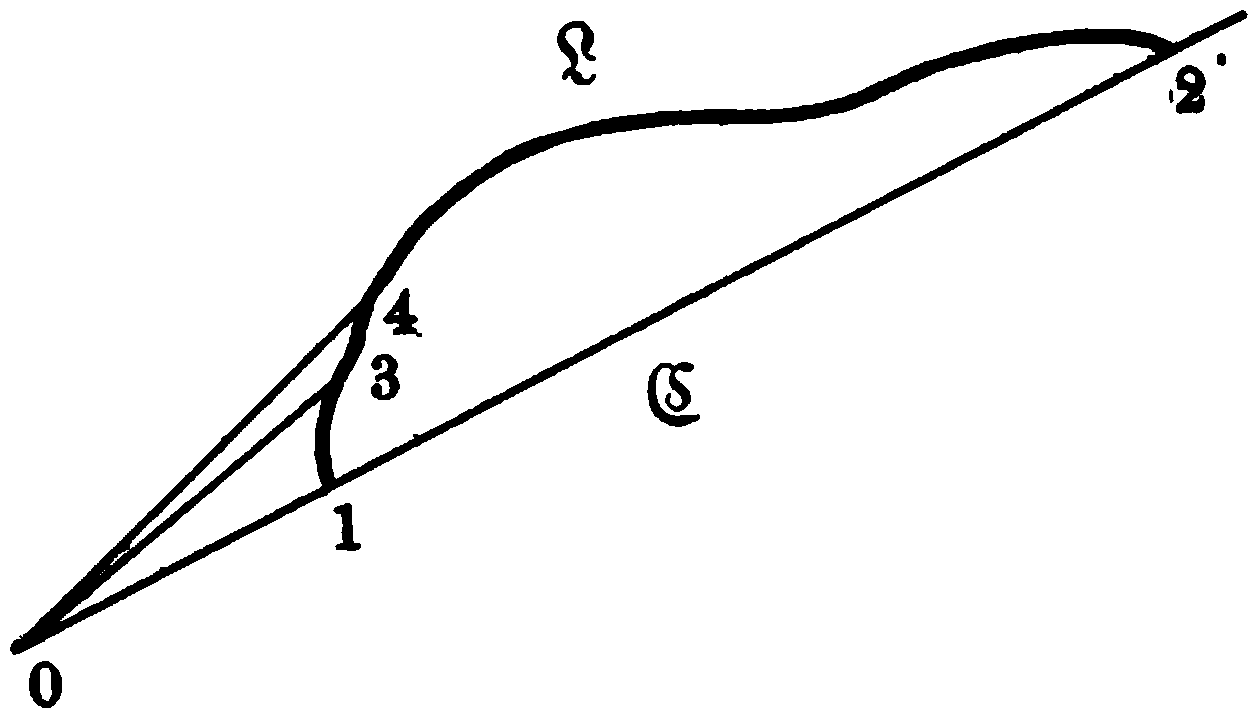
\includegraphics[width=\linewidth,height=30mm,keepaspectratio]{fig_assets/fig15_src_clean_x8.png}\par\vspace{1mm}
\end{minipage}
\end{center}

Ist also der Punkt 4 hinreichend nahe bei 3 gelegen (Fig.~15) und $\alpha$ ein hinreichend kleiner vorgeschriebener Werth, so kann man die Punkte 0 und 4 durch eine solche Extremale des Feldes verbinden, dass das längs dieser gebildete Integral $\overline{K}_{04}$ den Werth $\omega_3+\alpha$ hat. Setzt man speciell
\[
\alpha=K_{34},
\]
indem das Integral längs der Curve $\Omega$ gebildet wird, so sind alle Argumente der Ausdrücke (13), mithin auch die erhaltenen Werthe von $a$ und $b$ solche Functionen von $\tau$, wie sie in \S~17 durch $\varphi(\tau)$ bezeichnet wurden. Dabei gilt für die beiden Extremalen 03 und 04 die Beziehung
\[
\overline{K}_{04}=\overline{K}_{03}+K_{34},
\]
und hieraus folgt
\[
\overline{K}_{03}+K_{32}=\overline{K}_{04}+K_{42}.
\]
Lassen wir also den Punkt 3 in eine benachbarte Lage übergehen und verbinden ihn in dieser mit dem Punkte 0 durch die definirte Extremale 03, so bleibt die Grösse $\overline{K}_{03}+K_{32}$ constant. Können wir den Punkt 3 in dieser Weise den ganzen Bogen $\Omega$
% src-pdfpage=0155
% src-break=0155
durchlaufen lassen und ist $\mathfrak{C}$ die Anfangs- und Endlage der construirten Extremale 03, so sagen wir, die \textsc{Weierstrass}'sche Construction sei möglich. Die Grössen $a,b$, die zu der Extremale 03 gehören, sind dann in dem ganzen Intervall von $\tau_1$ bis $\tau_2$ Functionen von $\tau$ mit den Eigenschaften der Grössen $\varphi(\tau)$ des \S~17; ihre Anfangs- und Endwerthe sind $a_0,b_0$, während die constante Grösse $\overline{K}_{03}+K_{32}$ für $\tau=\tau_1$ und $\tau=\tau_2$ die Werthe
\[
\overline{K}_{01}+K_{12},
\quad
\overline{K}_{02}=\overline{K}_{01}+\overline{K}_{12}
\]
annimmt, welche nach (12) gleich sind. Bei speciellen Aufgaben kann die \textsc{Weierstrass}'sche Construction oft als möglich erkannt werden; eine allgemeine Bedingung ihrer Durchführbarkeit entwickeln wir in \S~38.

Um nun der Frage nach dem Extremum des Integrals $J$ näher zu kommen, bilden wir, die \textsc{Weierstrass}'sche Construction als möglich vorausgesetzt, die Grösse
\[
W=\overline{J}_{03}+J_{32},
\]
indem das erste Integral längs der construirten Extremale 03, das zweite längs der Curve $\Omega$ gebildet wird. Diese Grösse ist eine Function $\varphi(\tau)$ im Sinne des \S~17, und da die Extremale 03 schliesslich in die Lage $\mathfrak{C}$ übergeht, so hat man
\[
W\bigg|_{\tau_1}=\overline{J}_{01}+J_{12},
\quad
W\bigg|_{\tau_2}=\overline{J}_{01}+\overline{J}_{12}=\overline{J}_{02}.
\]
Gelingt es daher, das Vorzeichen der Grösse $dW$ als fest nachzuweisen, so ist die Differenz $\overline{J}_{12}-J_{12}$ von demselben Vorzeichen. Die Grösse $dW$ ist aber nach den Formeln des \S~35 explicite anzugeben; da nämlich $\overline{K}_{03}+K_{32}$ constant, also
\[
\frac{d(\overline{K}_{03}+K_{32})}{d\tau}=0
\]
ist, so hat man
\[
\frac{dW}{d\tau}=\frac{d\overline{J}_{03}}{d\tau}+\lambda\frac{d\overline{K}_{03}}{d\tau}
+\frac{dJ_{32}}{d\tau}+\lambda\frac{dK_{32}}{d\tau},
\]
wobei $\lambda$ die isoperimetrische Constante der Extremale 03 sei. Mit Benutzung der Formel (11) und der offenbar richtigen Gleichungen
\[
\frac{dJ_{32}}{d\tau}=-F\left(x,y,\frac{dx}{d\tau},\frac{dy}{d\tau}\right),
\quad
\frac{dK_{32}}{d\tau}=-G\left(x,y,\frac{dx}{d\tau},\frac{dy}{d\tau}\right)
\]
ergiebt sich hieraus
% src-pdfpage=0156
% src-break=0156
\begin{equation}\tag{14}
\frac{dW}{d\tau}=H_{x'}(x,y,\xi_t,\eta_t)\frac{dx}{d\tau}
+H_{y'}(x,y,\xi_t,\eta_t)\frac{dy}{d\tau}
-H\left(x,y,\frac{dx}{d\tau},\frac{dy}{d\tau}\right).
\end{equation}
Dieser Ausdruck ist identisch mit dem früher durch
\[
\frac{1}{d\tau}\mathfrak{E}(x,y,x',y',Dx,Dy)=
\mathfrak{E}\left(x,y,x',y',\frac{dx}{d\tau},\frac{dy}{d\tau}\right)
\]
bezeichneten, in welchem $F$ durch $H$ ersetzt ist; die oben (\S~21) abgeleiteten Eigenschaften von $\mathfrak{E}$ können daher benutzt und besonders das ordentliche und ausserordentliche Verschwinden unterschieden werden. Hat $\mathfrak{E}$ stets ein constantes Vorzeichen, und verschwindet längs keiner der in Betracht gezogenen Curven $\Omega$ überall, so wird das gesuchte Extremum des Integrals $J$ durch den Bogen 12 wirklich geliefert.

Wenn $\mathfrak{E}$ längs eines endlichen Theiles der Curve $\Omega$ überall ordentlich verschwände, so hätte man längs desselben
\[
\frac{dx}{d\tau}=m\xi_t,
\quad
\frac{dy}{d\tau}=m\eta_t,
\quad
m>0;
\]
da aber auch die Gleichungen
\[
x=\xi,
\quad
 y=\eta
\]
nach $\tau$ differenziirt werden können, so ergiebt sich
\begin{equation}\tag{15}
\begin{aligned}
\xi_t\frac{dt}{d\tau}+\xi_a\frac{da}{d\tau}+\xi_b\frac{db}{d\tau}&=m\xi_t,\\
\eta_t\frac{dt}{d\tau}+\eta_a\frac{da}{d\tau}+\eta_b\frac{db}{d\tau}&=m\eta_t.
\end{aligned}
\end{equation}
Ferner ist offenbar
\[
\frac{d\omega}{d\tau}=\omega_t\frac{dt}{d\tau}+\omega_a\frac{da}{d\tau}+\omega_b\frac{db}{d\tau},
\quad
\omega_t=G(\xi,\eta,\xi_t,\eta_t);
\]
da nun $\overline{K}_{03}+K_{32}$ von $\tau$ unabhängig ist, so folgt
\[
\frac{d\overline{K}_{03}}{d\tau}=-\frac{dK_{32}}{d\tau}=\frac{d\omega}{d\tau}=G\left(\xi,\eta,\frac{dx}{d\tau},\frac{dy}{d\tau}\right)
=mG(\xi,\eta,\xi_t,\eta_t)=m\omega_t,
\]
oder
\[
\frac{d\omega}{d\tau}=\omega_t\frac{dt}{d\tau}+\omega_a\frac{da}{d\tau}+\omega_b\frac{db}{d\tau}=m\omega_t.
\]
Diese Gleichung kann aber mit den unter (15) angeführten als homogen linear in den Grössen
% src-pdfpage=0157
% src-break=0157
\[
\frac{da}{d\tau},
\quad
\frac{db}{d\tau},
\quad
\frac{dt}{d\tau}-m
\]
angesehen werden; da nun die Determinante der Coëfficienten mit $\Delta$ identisch, also von Null verschieden ist, so können die drei Gleichungen nur zusammen bestehen, wenn
\[
\frac{da}{d\tau}=\frac{db}{d\tau}=0.
\]
Hieraus aber würde, da $a$ und $b$ durch die \textsc{Weierstrass}'sche Construction als Functionen $\varphi(\tau)$ im Sinne des \S~17 bestimmt sind, wenn 3 und 4 irgend zwei Punkte des betrachteten Bogens sind, folgen
\[
a\bigg|_4^3=b\bigg|_4^3=0;
\]
der Bogen wäre also ein Theil einer Extremale des Feldes. Verschwände $\mathfrak{E}$ längs der ganzen Curve $\Omega$ in ordentlicher Weise, so müsste, da $a_0,b_0$ die Endwerthe von $a,b$ sind, $\Omega$ mit $\mathfrak{C}$ zusammenfallen. Ist dies nicht der Fall, und ist ein ausserordentliches Verschwinden von $\mathfrak{E}$, sowie ein Zeichenwechsel entweder überhaupt oder durch Beschränkung der verglichenen Curven $\Omega$ ausgeschlossen, so ist die Differenz
\[
W\bigg|_{\tau_1}^{\tau_2}=\int_{\tau_1}^{\tau_2}\mathfrak{E}\,d\tau=\overline{J}_{12}-J_{12}
\]
von Null verschieden und hat das Vorzeichen mit $\mathfrak{E}$ gemein, womit das Extremum gesichert ist.

Im Ganzen sind somit drei Bedingungen als hinreichend für den Eintritt des Extremums nachgewiesen, 1) die Existenz eines Feldes oder die \textsc{Jacobi}'sche Bedingung, 2) die \textsc{Weierstrass}'sche Vorzeichenbedingung, d.~h. das in dem angegebenen Sinne feste Vorzeichen der Grösse $\mathfrak{E}$, 3) die Möglichkeit der \textsc{Weierstrass}'schen Construction innerhalb des Feldes. Sind diese Bedingungen erfüllt, so liefert die Extremale $\mathfrak{C}$ ein Extremum des Integrals $J_{12}$ gegenüber den im Felde verlaufenden Curven 12 oder $\Omega$, welche einen vorgeschriebenen Werth $K_{12}$ ergeben. Je nachdem das Vorzeichen von $\mathfrak{E}$ überhaupt gesichert ist oder nur, wenn $\Omega$ in engerer Nachbarschaft der Curve $\mathfrak{C}$ liegt, ist das Extremum stark oder schwach.

Dabei wird das Extremum im Allgemeinen nicht von dem im Punkte 0 beginnenden Bogen geliefert, sondern von dem
% src-pdfpage=0158
% src-break=0158
Bogen 12, dessen Anfangspunkt 1 beliebig nahe an die Lage 0 heranrücken kann.

Ersetzt man übrigens in der allgemeinen Untersuchung des \S~21 die Function $F$ durch $H$, so sieht man, dass die hier betrachtete Grösse $\mathfrak{E}$ ein festes Vorzeichen besitzt, sobald dasselbe von der Grösse
\[
H_1=\frac{1}{y'^2}H_{x'x'}=\frac{1}{x'^2}H_{y'y'}=
\frac{1}{x'^2}(F_{y'y'}+\lambda G_{y'y'})
\]
oder auch, wenn $x'$ nicht verschwindet, von dem Product $(f_{pp}+\lambda g_{pp})dx$ gilt. Die \textsc{Weierstrass}'sche Vorzeichenbedingung kann daher durch die \textsc{Legendre}'sche des \S~17 ersetzt werden, wenn man in dieser $F+\lambda G$ an Stelle von $F$ treten lässt.

Sind die Bedingungen 1) und 2) erfüllt, so bleiben sie erfüllt für die Aufgabe, welche man erhält, indem man die Integrale $J,K$ ihre bisherigen Rollen vertauschen lässt. Für die Bedingung 1) folgt dies unmittelbar aus den obigen Bemerkungen, wonach die Eigenschaft gewisser Extremalen, ein Feld zu bilden, bei jener Vertauschung erhalten bleibt. Analoges ergiebt sich für die Bedingung 2) daraus, dass $H$ und $\mathfrak{E}$ durch
\[
G+\frac{1}{\lambda}F,
\quad
\frac{1}{\lambda}\mathfrak{E}
\]
ersetzt werden; letztere Grösse hat offenbar, da $\lambda$ von Null verschieden ist, ein festes Vorzeichen, wenn dies von $\mathfrak{E}$ gilt, wobei freilich das Vorzeichen nicht das der Grösse $\mathfrak{E}$ zu sein braucht. Das Extremum hat daher in der neuen Aufgabe denselben Charakter wie in der alten, oder den entgegengesetzten, je nachdem $\lambda$ positiv oder negativ ist. Damit ist der einfachste Fall eines von \textsc{Mayer} aufgestellten Reciprocitätsgesetzes bewiesen.



% machine-unit: Kneser_LVR_DE_p0158low_p0177top §§37-39
% visible source begins below §37 on source pdfpage 0158; p0177 §40 heading/body excluded from this slice.

% src-pdfpage=0158
% src-break=0158
\begin{center}
{\large \S~37.}
\end{center}

\noindent\textbf{Beispiel. Aufgabe IX (\S~34).} Die Extremalen sind Kreise vom Radius $\pm\lambda$; die durch einen Punkt 0, z.~B. den Coordinatenanfangspunkt gehenden können in folgender Weise dargestellt werden. Es seien $a,b$ die Coordinaten des Mittelpunktes $m$, der Radius sei $r$ (Fig.~16); dann kann man setzen
\begin{equation}\tag{16}
 x=a+r\cos\theta,\quad y=b+r\sin\theta,\quad r^2=a^2+b^2
\end{equation}
und $\theta$ ist der Winkel, den der Radius, von der zur $+x$-Axe parallelen Lage $mx$ ausgehend, im positiven Drehungssinne beschreiben muss, um seinen Endpunkt in den jeweils betrachteten Punkt 4 des Kreises zu bringen; positiv ist, wie gewöhnlich, derjenige Drehungssinn, welcher nach einer Drehung um $90^\circ$ die
% src-pdfpage=0159
% src-break=0159
$+x$-Axe in die $+y$-Axe überführt.

\begin{center}
\begin{minipage}{0.48\linewidth}\centering
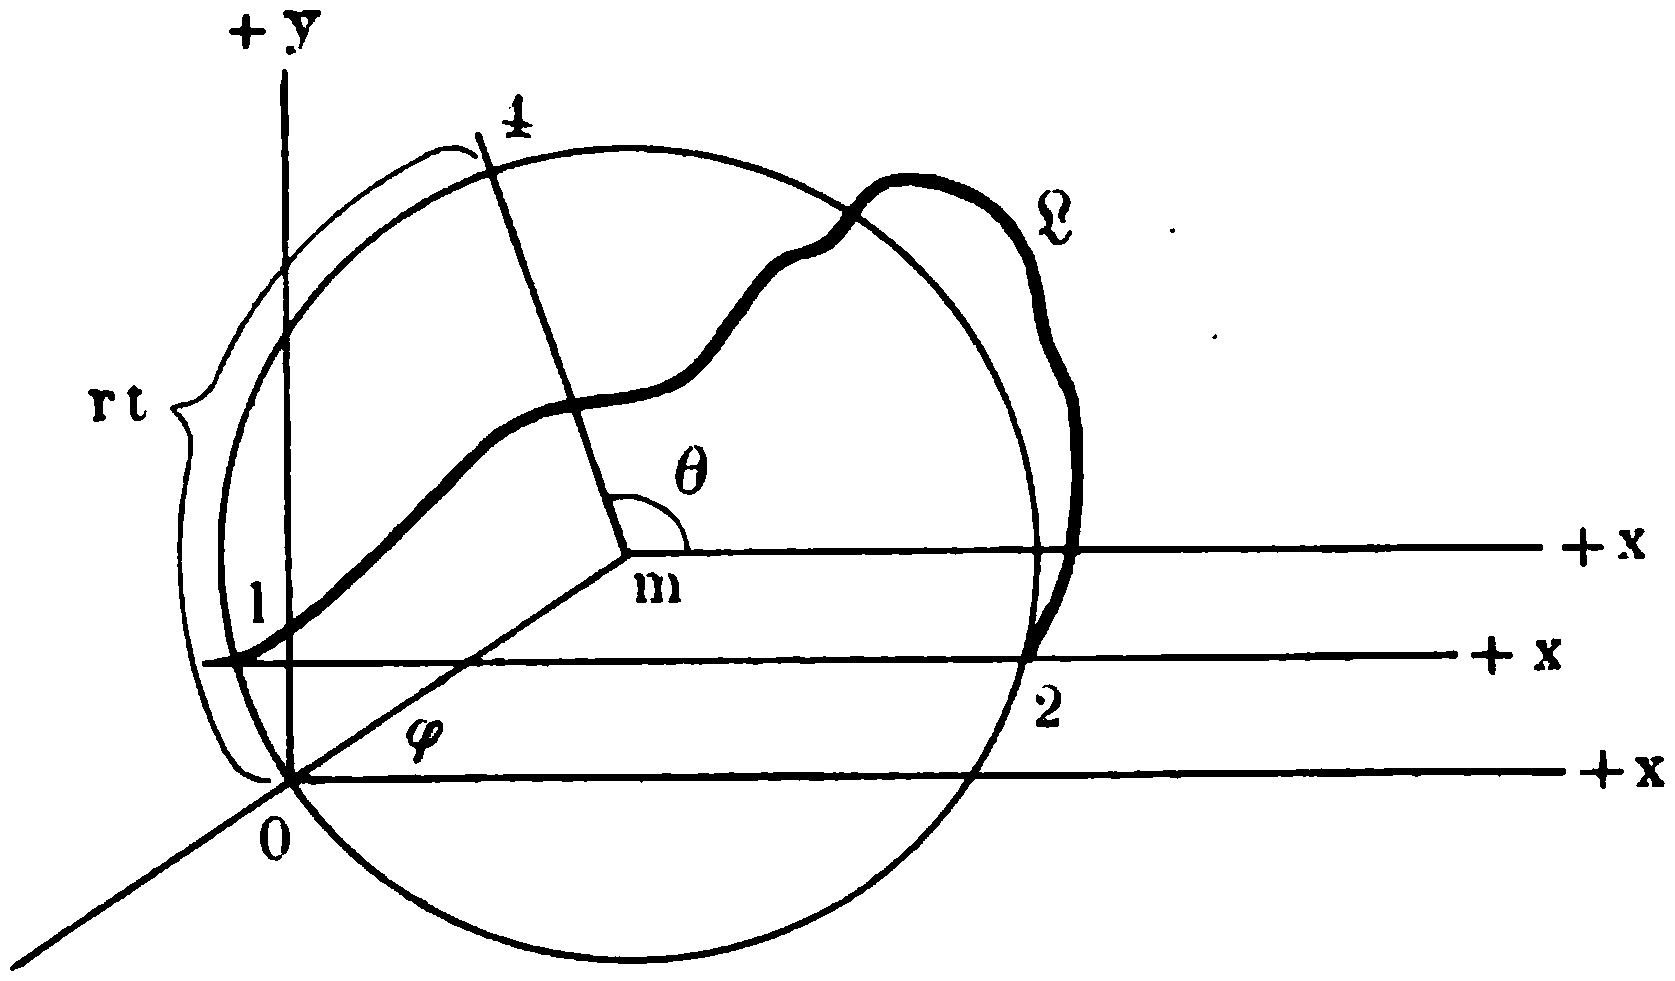
\includegraphics[width=\linewidth,height=36mm,keepaspectratio]{fig_assets/fig16_p0159_src_clean_x8.png}\par\vspace{1mm}
\end{minipage}
\end{center}

Ist ferner $\varphi$ der Winkel, um welchen der Strahl $0m$, im positiven Sinne gemessen, von der $+x$-Axe abweicht, so hat man
\begin{equation}\tag{17}
 a=r\cos\varphi,\quad b=r\sin\varphi,
\end{equation}
und der Radius $m0$ ist demnach um $\varphi+\pi$ gegen $mx$ geneigt. Setzt man daher
\[
 t=\pi+\varphi-\theta,\quad \theta=\pi+\varphi-t,
\]
so ist $rt$ der im negativen Sinne vom Punkte 0 ab gemessene Kreisbogen 04 und man hat nach (16), (17)
\[
 K_{04}=\omega=t\sqrt{a^2+b^2},\quad
 \xi(t,a,b)=a-a\cos t-b\sin t,
\]
\[
 \eta(t,a,b)=b-b\cos t+a\sin t.
\]
Diese Functionen sind überall regulär, so lange $r$ zwischen zwei übrigens ganz beliebigen positiven Grenzen verbleibt. Man hat ferner
\[
\Delta=\begin{vmatrix}
1-\cos t&\sin t&\dfrac{at}{r}\\[1.0ex]
-\sin t&1-\cos t&\dfrac{bt}{r}\\[1.0ex]
a\sin t-b\cos t&a\cos t+b\sin t&r
\end{vmatrix},
\]
und wenn man $a$ und $b$ durch andere Variable $\alpha,\beta$ ausdrückt,
\begin{equation}\tag{18}
\frac{\partial(\xi,\eta,\omega)}{\partial(t,\alpha,\beta)}=
\frac{\partial(\xi,\eta,\omega)}{\partial(t,a,b)}\cdot
\frac{\partial(t,a,b)}{\partial(t,\alpha,\beta)}
=\Delta\frac{\partial(a,b)}{\partial(\alpha,\beta)};
\end{equation}
sind speciell $\alpha,\beta$ die rechtwinkeligen Coordinaten des Punktes $m$ in einem neuen System, so hat der Factor neben $\Delta$ den Werth
% src-pdfpage=0160
% src-break=0160
$\pm1$. Wenn nun speciell $b=0$ ist, so hat man $a^2=r^2$, und es ist
\[
\begin{aligned}
\Delta&=r\begin{vmatrix}
1-\cos t&\sin t&t\\
-\sin t&1-\cos t&0\\
\sin t&\cos t&1
\end{vmatrix}\\
&=r(2-2\cos t-t\sin t)=4r\sin\frac{t}{2}\left(\sin\frac{t}{2}-\frac{t}{2}\cos\frac{t}{2}\right).
\end{aligned}
\]
Durchläuft aber der Punkt 4 den betrachteten Kreis, so bewegt sich $t$ in dem Intervall
\begin{equation}\tag{19}
0\leq t<2\pi,
\end{equation}
die Factoren des Ausdrucks $\Delta$ sind also, abgesehen vom Punkte 0, von Null verschieden. Verschwindet $b$ nicht, so ersetze man das Coordinatensystem $(a,b)$ durch ein neues $(\alpha,\beta)$, dessen Abscissenaxe durch $m$ geht; dann bleibt $\Delta$ nach der Formel (18) ebenfalls von Null verschieden. Damit ist gezeigt, dass alle Kreise, die durch den Punkt 0 gehen und, wenn $\varepsilon,\gamma$ positive Constante bedeuten, einer Ungleichung
\begin{equation}\tag{20}
\varepsilon^2<a^2+b^2<\gamma^2
\end{equation}
unterworfen sind, ein Feld im Sinne des \S~36 bilden, sobald man $t$ durch die Ungleichung (19) beschränkt, d.~h. keinen der Kreise mehr als einmal durchlaufen denkt.

Da bei dieser Aufgabe
\[
F=yx',\quad G=\sqrt{x'^2+y'^2},\quad H=yx'+\lambda\sqrt{x'^2+y'^2},
\]
und die Quadratwurzeln positiv sind, so hat man
\[
\begin{aligned}
\mathfrak{E}&=\left(y+\frac{\lambda x'}{\sqrt{x'^2+y'^2}}\right)Dx+
\frac{\lambda y'}{\sqrt{x'^2+y'^2}}Dy-
\left(yDx+\lambda\sqrt{Dx^2+Dy^2}\right)\\
&=\lambda\sqrt{Dx^2+Dy^2}\left\{\frac{x'}{\sqrt{x'^2+y'^2}}\frac{Dx}{\sqrt{Dx^2+Dy^2}}+
\frac{y'}{\sqrt{x'^2+y'^2}}\frac{Dy}{\sqrt{Dx^2+Dy^2}}-1\right\};
\end{aligned}
\]
die eingeklammerte Grösse ist (\S~23, Aufgabe I) nie positiv, und $\mathfrak{E}$ verschwindet nur, wenn
\[
\frac{x'}{\sqrt{x'^2+y'^2}}=\frac{Dx}{\sqrt{Dx^2+Dy^2}},\quad
\frac{y'}{\sqrt{x'^2+y'^2}}=\frac{Dy}{\sqrt{Dx^2+Dy^2}},
\]
d.~h. nur in ordentlicher Weise. Da ferner die Richtung wachsender $t$ zum auswärts gerichteten Radius so liegt, wie die
% src-pdfpage=0161
% src-break=0161
$+x$-Axe zur $+y$-Axe, so ist $\lambda$ nach \S~34 negativ, also $\mathfrak{E}$ positiv, und das gesuchte Extremum ein Maximum.

Jetzt seien die Punkte 12 durch einen Bogen eines Kreises verbunden; ausserhalb dieses Bogens liege auf dem Kreise der Punkt 0. Durch diesen werde die Abscissenaxe parallel zur Geraden 12 gezogen und die $y$-Axe so gelegt, dass auf dieser Geraden $y$ positiv ist. Dann führt die oben definirte Richtung wachsender $t$ von 1 durch den Bogen $\mathfrak{C}$ zum Punkte 2, und das Integral
\[
\overline{J}_{12}=\int_1^2 yx'\,dt
\]
ist die positive Fläche zwischen $\mathfrak{C}$ und der geraden Strecke 12, vermehrt um das von den Ordinaten der letzteren bedeckte Rechteck. Es sei ferner $\Omega$ eine beliebige 1 und 2 verbindende Curve von denselben Stetigkeitseigenschaften wie in \S~17 und derselben Länge wie $\mathfrak{C}$, welche nicht in einen Kreis mit dem Radius $2\varepsilon$ und dem Centrum 0 hineingeht, was durch passende Wahl dieses Punktes stets zu erreichen ist. Dann haben alle Kreise, welche durch 0 und einen der Curve $\Omega$ angehörigen Punkt 3 gehen, einen Radius, der grösser als $\varepsilon$ ist. Beschränkt man sich auf solche, deren Radien eine gewisse Grenze $\gamma$ nicht überschreiten, so gehören sie alle dem Felde (20) an.

Durchläuft nun der Punkt 3 den Bogen $\Omega$, so verbinde man ihn in jeder seiner Lagen mit 0 durch einen Kreisbogen von der Länge
\[
\overline{K}_{01}+K_{13}=\operatorname{arc}01+\operatorname{arc}13,
\]
wobei der erste Bogen auf dem Kreise 012, der zweite auf der Curve $\Omega$ gemessen wird. Diese Grösse ist grösser als der geradlinige Abstand 03, man erhält daher für den gesuchten Bogen einen endlichen Radius, und, da er sich offenbar mit 3 stetig verändert, eine endliche obere Grenze $\gamma$. Von den beiden zur Geraden 03 symmetrisch gelegenen Kreisbögen der verlangten Beschaffenheit nehmen wir immer den, der aus der Anfangslage $\mathfrak{C}$ stetig hervorgeht; da der Radius endlich bleibt, ist $\mathfrak{C}$ auch die Endlage des Bogens 03 und die \textsc{Weierstrass}'sche Construction innerhalb des Feldes (20) in vollem Umfange als möglich erwiesen. Die allgemeine Theorie des \S~36 ergiebt daher
\[
\overline{J}_{12}>J_{12},
\]
d.~h. das vom Kreisbogen $\mathfrak{C}$ und der geraden Strecke 12 be-
% src-pdfpage=0162
% src-break=0162
grenzte Segment ist grösser als das durch die Curve $\Omega$ definirte. Damit ist offenbar noch mehr als die Maximumseigenschaft erwiesen.

\begin{center}
{\large \S~38.}
\end{center}

Die \textsc{Weierstrass}'sche Construction ist ausführbar, wenn man der Curve $\Omega$ eine Beschränkung auferlegt, die bei vielen Aufgaben naturgemäss erscheint, und darin besteht, dass in benachbarten Punkten der Curven $\Omega$ und $\mathfrak{C}$ auch die vom Punkte 0 aus längs beider Curven gebildeten Integrale $K$ nur wenig von einander abweichen. Um diese Festsetzung genauer zu formuliren, nehmen wir an, eine beliebige, vom Punkte 0 ausgehende Curve werde vom Punkte 6 durchlaufen, $K_{06}$ sei das längs dieser Curve erhaltene Integral, und $z$ sei die dritte der rechtwinkeligen Raumcoordinaten. Setzen wir dann allgemein
\[
x=x_6,\quad y=y_6,\quad z=K_{06},
\]
so beschreibt der Punkt $(x,y,z)$ eine gewisse, ebenfalls vom Punkte 0 ausgehende Raumcurve; die auf diese Weise irgend welchen Punkten $1,\ldots,6$ zugeordneten Punkte des Raumes seien durch $1^0,\ldots,6^0$ bezeichnet. Es entspricht dann jeder Extremale des Feldes eine Curve
\[
x=\xi(t,a,b),\quad y=\eta(t,a,b),\quad z=\omega(t,a,b);
\]
für $a=a_0,b=b_0$ erhält man eine der Curve $\mathfrak{C}$ entsprechende Raumcurve $\mathfrak{C}^0$. Der aus dem Extremalenbogen 01 und der Curve $\Omega$ zusammengesetzten Linie entspricht eine Raumcurve, welche bis zum Punkte $1^0$, dessen Coordinaten
\[
x=x_1,\quad y=y_1,\quad z=\overline{K}_{01}=\omega(t_1,a_0,b_0)
\]
sind, mit $\mathfrak{C}^0$ zusammenfällt, dann sich aber von dieser trennt; der Punkt $3^0$ hat die Coordinaten
\begin{equation}\tag{21}
x=x_3,\quad y=y_3,\quad z=\overline{K}_{01}+K_{13}.
\end{equation}
Die neue Festsetzung besteht nun darin, dass nur diejenigen Curven $\Omega$ mit $\mathfrak{C}$ hinsichtlich der Werthe des Integrals $J$ verglichen werden, deren zugehörige Raumcurven $\Omega^0$ einer gewissen Nachbarschaft (\S~17) der Curve $\mathfrak{C}^0$ angehören.

Auf der letzteren entspreche einem Punkte 5 des Bogens 12 der Punkt $5^0$, für welchen
\[
x=x_5,\quad y=y_5,\quad z=\overline{K}_{05}=\omega(t_5,a_0,b_0)=z_5;
\]
dann können die Gleichungen
% src-pdfpage=0163
% src-break=0163
\begin{equation}\tag{22}
\begin{aligned}
x-x_5&=\xi(t,a,b)-x_5=[t-t_5,a-a_0,b-b_0]_1,\\
y-y_5&=\eta(t,a,b)-y_5=[t-t_5,a-a_0,b-b_0]_1,\\
z-z_5&=\omega(t,a,b)-z_5=[t-t_5,a-a_0,b-b_0]_1,
\end{aligned}
\end{equation}
in welchen die linearen Glieder rechts die Determinante $\Delta(t_5,a_0,b_0)$ haben, dadurch erfüllt werden, dass man für $t-t_5,a-a_0,b-b_0$, gewisse bestimmte Reihen von der Form
\[
[x-x_5,\ y-y_5,\ z-z_5]_1
\]
einsetzt. Diese Ausdrücke definiren $t,a,b$ als Functionen von $x,y,z$, welche an jeder Stelle $5^0$ regulär sind, welche daher, wenn die Curve $\mathfrak{C}$ sich selbst nicht schneidet, also zu verschiedenen Werthen $t_5$ auch verschiedene Punkte $5^0$ gehören, innerhalb eines gewissen, den Bogen $1^02^0$ umfassenden Gebietes $\mathfrak{G}^0$ regulär und eindeutig bestimmt sind, so dass dasselbe von den Extremalen, welche den durch die obigen Ausdrücke definirten $a,b$ entsprechen, genau einfach erfüllt wird. Fällt der betrachtete Punkt auf die Curve $\mathfrak{C}^0$ selbst, so gehen $a$ und $b$ in $a_0$ und $b_0$ über. Das Gebiet $\mathfrak{G}^0$ kann man sich z.~B. als den Raum vorstellen, den eine Kugel von constantem Radius durchstreicht, wenn ihr Mittelpunkt den Bogen $1^02^0$ durchläuft.

Verläuft nun die Curve $\Omega^0$ ganz im Inneren des Gebietes $\mathfrak{G}^0$, so liegt jeder Punkt $3^0$ auf einer bestimmten der definirten Extremalen des Feldes, und man hat die Gleichungen
\[
x_3=\xi(t_3,a,b),\quad y_3=\eta(t_3,a,b),\quad z_3=\omega(t_3,a,b).
\]
Hieraus folgt nach der dritten Gleichung (21)
\[
\omega(t_3,a,b)=\overline{K}_{03}=\overline{K}_{01}+K_{13},
\]
mithin
\[
\overline{K}_{03}+K_{32}=\overline{K}_{01}+K_{13}+K_{32}=\overline{K}_{01}+K_{12}=\overline{K}_{02};
\]
die Projection der construirten Curve $03^0$ auf die $xy$-Ebene ist also genau die bei der \textsc{Weierstrass}'schen Construction gesuchte Extremale 03 und sie geht nach den an die Gleichungen (22) geknüpften Bemerkungen in $\mathfrak{C}$ über, wenn der Punkt $3^0$ in eine der Lagen $1^0$ und $2^0$ rückt. Bei der neu eingeführten Beschränkung der Curven $\Omega$ ist also die \textsc{Weierstrass}'sche Construction immer möglich, und eine der in \S~36 angegebenen hinreichenden Bedingungen des Extremums fällt weg.

\noindent\textbf{Beispiel. Aufgabe XI.} Einen schweren homogenen Faden von gegebener Länge und gegebenen Endpunkten in einer verticalen
% src-pdfpage=0164
% src-break=0164
 Ebene so zu legen, dass sein Schwerpunkt möglichst tief liegt (Gleichgewichtsfigur, Kettenlinie).

Ist die $+y$-Axe die Richtung der Schwere, $l$ die Länge des Fadens 01, die Masse der Längeneinheit Eins, so ist die Ordinate des Schwerpunktes
\[
\frac{1}{l}\int_0^1 y\sqrt{x'^2+y'^2}\,dt,
\]
es ist also das Integral
\[
J=\int_0^1 y\sqrt{x'^2+y'^2}\,dt
\]
zum Maximum zu machen bei vorgeschriebenem Werth des Bogenintegrals
\[
K=\int_0^1 \sqrt{x'^2+y'^2}\,dt,
\]
und die erste Variation des Integrals
\[
J+\lambda K=\int (y+\lambda)\sqrt{x'^2+y'^2}\,dt
\]
ist gleich Null zu setzen. Für die Extremalen erhält man hieraus (\S~9, Aufgabe II) die Gleichung
\[
y+\lambda=\frac{a}{2}\left\{e^{\frac{x-b}{a}}+e^{-\frac{x-b}{a}}\right\}=a\Cof\frac{x-b}{a}.
\]
Die rechte Seite hat für $x=\pm\infty$ das Vorzeichen der Grösse $a$, die Curve ist also convex nach unten für $a<0$. Dann ist $y+\lambda$ immer negativ, und die Grösse
\[
\mathfrak{E}=(y+\lambda)\sqrt{Dx^2+Dy^2}\left\{\frac{x'Dx+y'Dy}{\sqrt{x'^2+y'^2}\sqrt{Dx^2+Dy^2}}-1\right\}
\]
positiv, und nur dann $=0$, wenn die Werthsysteme $(x',y')$ und $(Dx,Dy)$ dieselbe Richtung darstellen. Die \textsc{Weierstrass}'sche Vorzeichenbedingung des starken Maximums ist also erfüllt.

Die weitere Rechnung vereinfacht sich vermittelst der leicht zu beweisenden Formeln
\begin{equation}\tag{23}
\begin{aligned}
\Cof(u+v)&=\Cof u\Cof v+\Sin u\Sin v,\\
\Sin(u+v)&=\Sin u\Cof v+\Sin v\Cof u.
\end{aligned}
\end{equation}
Für die Constanten der durch den festen Punkt 0 gehenden Extremalen gilt die Beziehung
\[
y_0+\lambda=a\Cof\frac{x_0-b}{a},
\]
% src-pdfpage=0165
% src-break=0165
und die allgemeine Gleichung dieser Curvenschar kann demnach geschrieben werden
\[
y-y_0=a\left\{\Cof\frac{x-b}{a}-\Cof\frac{x_0-b}{a}\right\}.
\]
Die rechte Seite dieser Gleichung ist regulär, sobald $a$ von Null verschieden ist, und man kann setzen
\[
x=\xi(t,a,b)=t,\quad y=\eta(t,a,b)=y_0+a\left\{\Cof\frac{t-b}{a}-\Cof\frac{t_0-b}{a}\right\}.
\]
Da nun
\[
\xi_t=1,\quad \xi_a=\xi_b=0,
\]
so ist
\[
\Delta(t,a,b)=\frac{\partial(\xi,\eta,\omega)}{\partial(t,a,b)}=\frac{\partial(\eta,\omega)}{\partial(a,b)}.
\]
Weiter ist $\omega$ die vom Punkte 0 ab gemessene Bogenlänge, also
\[
\omega=\int_0^t\sqrt{1+y'^2}\,dt=\int_0^t\sqrt{1+\Sin^2\frac{t-b}{a}}\,dt
=\int_0^t \Cof\frac{t-b}{a}\,dt,
\]
\[
=a\left\{\Sin\frac{t-b}{a}-\Sin\frac{t_0-b}{a}\right\};
\]
man erhält daher, wenn
\[
\frac{t-b}{a}=u,
\quad
\frac{t_0-b}{a}=u_0
\]
gesetzt wird, auf Grund der Formeln für die Differentiale der hyperbolischen Functionen (\S~23)
\[
-\Delta=\begin{vmatrix}
\Cof u-\Cof u_0-(u\Sin u-u_0\Sin u_0)&\Sin u-\Sin u_0\\
\Sin u-\Sin u_0-(u\Cof u-u_0\Cof u_0)&\Cof u-\Cof u_0
\end{vmatrix};
\]
differenzirt man ferner und benutzt die Gleichungen (23), so folgt
\[
\begin{aligned}
-\frac{d\Delta}{du}&=\begin{vmatrix}
-u\Cof u&\Sin u-\Sin u_0\\
-u\Sin u&\Cof u-\Cof u_0
\end{vmatrix}
+\begin{vmatrix}
\Cof u-u\Sin u-\Cof u_0+u_0\Sin u_0&\Cof u\\
\Sin u-u\Cof u-\Sin u_0+u_0\Cof u_0&\Sin u
\end{vmatrix}\\
&=(u-u_0)\Cof(u-u_0)-\Sin(u-u_0).
\end{aligned}
\]
Hieraus ergiebt sich
\[
-\frac{d^2\Delta}{du^2}=(u-u_0)\Sin(u-u_0);
\]
da die Grössen $u-u_0$ und $\Sin(u-u_0)$ dasselbe Vorzeichen haben, so ist immer
% src-pdfpage=0166
% src-break=0166
\[
\frac{d^2\Delta}{du^2}\leq0;
\]
da ferner die Grössen $\Delta$ und $d\Delta:du$ für $u=u_0$ verschwinden, so hat letztere stets das Vorzeichen von $u_0-u$, und erstere ist negativ, sobald $u\gtrless u_0$. Geht man nun vom Punkte 0 aus in der Richtung wachsender $x$ die Kettenlinie entlang, so ist
\[
u-u_0=\frac{x-x_0}{a}
\]
ebenso wie $a$ negativ, $\Delta$ also negativ; es sind daher für ein beliebig langes Stück der nach unten convexen Kettenlinie die hinreichenden Bedingungen des starken Maximums mit der oben angegebenen Beschränkung der Curven $\Omega$ erfüllt. Dabei ergiebt sich, gemäss einer in \S~36 gemachten Bemerkung, das Maximum zunächst für jeden Bogen 12, dessen Anfangspunkt beliebig nahe bei 0 liegt; da nun die Lage des letzteren keiner Beschränkung unterliegt, so kann der Bogen 12 als ein beliebiger Theil der Curve angesehen werden.

Die eingeführte Beschränkung der Curve $\Omega$ erscheint hier naturgemäss, weil bei jeder kleinen Verschiebung eines Fadens der einzelne materielle Punkt, der durch eine bestimmte, vom Punkte 0 ab gemessene Fadenlänge definirt ist, als nur wenig verschoben vorgestellt wird. Die Curven $\Omega$ und $\mathfrak{C}$ sind dann eindeutig so auf einander bezogen, dass entsprechende Punkte kleinen Abstand haben und denselben Werth des Integrals $K$ ergeben.

\begin{center}
{\large \S~39.}
\end{center}

Die allgemeinen Entwickelungen der letzten Paragraphen bleiben mit geringen Modificationen gültig, wenn man annimmt, dass die Extremalen
\begin{equation}\tag{24}
x=\xi(t,a,b),\quad y=\eta(t,a,b),
\end{equation}
zu welchen $\mathfrak{C}$ gehört, nicht durch einen festen Punkt 0 gehen, sondern alle eine feste Curve $\mathfrak{C}_0$ transversal schneiden; man erhält dann Kriterien dafür, dass ein Stück der Curve $\mathfrak{C}$ ein Extremum des Integrals liefere unter allen Curven, welche einen festen Punkt mit der Curve $\mathfrak{C}_0$ verbinden, und dem Integral $K$ einen vorgeschriebenen Werth geben.

Es sei
\[
\Gamma(x,y)=0
\]
% src-pdfpage=0167
% src-break=0167
die Gleichung der Curve $\mathfrak{C}_0$; dieselbe schneide $\mathfrak{C}$ und die von dieser hinreichend wenig abweichenden Curven der Schar (24) im variablen Punkte 0 unter nicht verschwindenden Winkeln, und sei in diesem Punkte regulär. Dann hat man die Gleichung
\begin{equation}\tag{25}
\Gamma[\xi(t_0,a,b),\eta(t_0,a,b)]=0,
\end{equation}
welche nach $t_0$ aufgelöst werden kann, da für die betrachteten Punkte 0 die Ungleichung
\[
\Gamma_x\xi_t+\Gamma_y\eta_t\neq0
\]
gilt. Man erhält daher, wenn $t_{00}$ der Parameter ist, welcher auf der Curve $\mathfrak{C}$ zum Schnittpunkt derselben mit $\mathfrak{C}_0$ gehört,
\[
t_0-t_{00}=[a-a_0,b-b_0]_1.
\]
Da ferner die Extremalen der Schar (24) die Curve $\mathfrak{C}_0$ transversal schneiden, so erhält man unter der Voraussetzung
\[
\left.\Gamma_xDx+\Gamma_yDy\right|^0=0
\]
immer die Gleichung
\[
\left.H_{x'}Dx+H_{y'}Dy\right|^0=0;
\]
daraus folgt
\begin{equation}\tag{26}
\left.\Delta=H_{x'}\Gamma_y-H_{y'}\Gamma_x\right|^0=0,
\end{equation}
wobei die Argumente
\begin{equation}\tag{27}
x=\xi,\quad y=\eta,\quad x'=\xi_t,\quad y'=\eta_t
\end{equation}
zu nehmen sind. Differenzirt man sodann die Gleichung (25) nach $a$ und $b$, so ergiebt sich
\[
\left.\Gamma_x\left(\xi_t\frac{\partial t_0}{\partial a}+\xi_a\right)+\Gamma_y\left(\eta_t\frac{\partial t_0}{\partial a}+\eta_a\right)\right|^0=0,
\]
\[
\left.\Gamma_x\left(\xi_t\frac{\partial t_0}{\partial b}+\xi_b\right)+\Gamma_y\left(\eta_t\frac{\partial t_0}{\partial b}+\eta_b\right)\right|^0=0.
\]
In diesen Gleichungen kann man nach (26) die Grössen $\Gamma_x$ und $\Gamma_y$ durch $H_{x'}$ und $H_{y'}$ ersetzen; sie werden dann genau mit den Formeln (9) identisch. Bildet man daher längs irgend einer Extremale der Schar, welcher der variable Punkt 3 angehört, die Integrale
\[
\overline{J}_{03}=\int_0^3 F\,dt=\int_{t_0}^{t}F(\xi,\eta,\xi_t,\eta_t)\,dt,\quad
\overline{K}_{03}=\int_{t_0}^{t}G(\xi,\ldots,\eta_t)\,dt,
\]
so gilt zunächst die von dem Zusammenhang zwischen $t_0,a,b$ unabhängige Gleichung (7) auch jetzt noch, und aus ihr folgen
% src-pdfpage=0168
% src-break=0168
genau wie in \S~35 auf Grund der Formel (9) die Gleichungen (10), (11).

Es werde nun wie oben
\[
\overline{K}_{03}=\omega(t,a,b)
\]
gesetzt und angenommen, dass die Determinante
\[
\Delta=\frac{\partial(\xi,\eta,\omega)}{\partial(t,a,b)}
\]
längs des der Curve $\mathfrak{C}$ angehörigen Bogens 02, abgesehen vom Punkte 0, nicht verschwinde; dann gilt dasselbe für alle auf der Curve $\mathfrak{C}_0$ beginnenden Bögen von Extremalen der Schar, welche von 02 hinreichend wenig abweichen; die Gesammtheit der Bögen, für welche $\Delta$ von Null verschieden bleibt, heisse das Feld des Bogens 02. Auf der Curve $\mathfrak{C}_0$ selbst verschwindet $\Delta$ überall, wie die Formeln (7), (9) leicht ergeben. Eine gewisse Umgebung des Bogens 02 wird dann, wie eine in \S~35 durchgeführte Betrachtung auch jetzt zeigt, von den Extremalen des Feldes im Allgemeinen unendlich vielfach bedeckt. Innerhalb dieser Umgebung werde ein der Curve $\mathfrak{C}_0$ angehöriger Punkt 1 mit 2 durch eine Linie $\Omega$ verbunden, für welche die Gleichung
\begin{equation}\tag{28}
K_{12}=\overline{K}_{02}
\end{equation}
besteht, auf deren rechter Seite längs der Curve $\mathfrak{C}$ integrirt ist, während die ungestrichenen Integrale sich auch jetzt stets auf die Curve $\Omega$ beziehen mögen. Diese werde vom Punkte 3 durchlaufen; dann besteht eine der \textsc{Weierstrass}'schen analoge Construction darin, dass eine mit 3 veränderliche Extremale des Feldes construirt wird, für welche die Grösse $\overline{K}_{03}+K_{32}$ constant bleibt, und welche, wenn die Punkte 3 und 2 zusammenfallen, in die Curve $\mathfrak{C}$ übergeht. Anfangs- und Endwerth dieser Grösse sind dann offenbar die beiden Seiten der Gleichung (28).

Der in \S~38 gegebene Beweis für die Möglichkeit der \textsc{Weierstrass}'schen Construction kann jedoch auf die vorliegende Aufgabe nicht ohne Weiteres übertragen werden, da $\Delta$ auf der Curve $\mathfrak{C}_0$, wie bemerkt, verschwindet. Dieser Umstand hat keinen Einfluss auf die Argumentation des \S~36, nach welcher $\mathfrak{E}$ nur längs einer Extremale des Feldes überall in ordentlicher Weise verschwinden kann; da nun die Grösse $\overline{K}_{03}+K_{32}$ von $\tau$ unabhängig ist, da ferner die Gleichungen (7), (10), (11) des \S~35, wie gezeigt, auch jetzt gelten, so ergiebt sich, wie in \S~36:
% src-pdfpage=0169
% src-break=0169
\[
\frac{dW}{d\tau}=\frac{d(\overline{J}_{03}+J_{32})}{d\tau}
=H_x\frac{dx}{d\tau}+H_y\frac{dy}{d\tau}-H\left(x,y,\frac{dx}{d\tau},\frac{dy}{d\tau}\right)
=\mathfrak{E}\left(x,y,x',y',\frac{dx}{d\tau},\frac{dy}{d\tau}\right).
\]
Die Anfangs- und Endwerthe der Grösse $W$ sind von den früheren verschieden; man hat offenbar jetzt
\[
\left.W\right|^{\tau_1}=J_{12},\quad \left.W\right|^{\tau_2}=\overline{J}_{02};
\]
die Differenz $\overline{J}_{02}-J_{12}$ hat also das Vorzeichen der Grösse $\mathfrak{E}$.

Schneiden daher die Extremalen des Feldes die reguläre Curve $\mathfrak{C}_0$ transversal, ohne sie zu berühren, so haben die in \S~36 angegebenen hinreichenden Bedingungen des Extremums dieselbe Bedeutung für das Extremum unter allen die Curve $\mathfrak{C}_0$ mit einem festen Punkte verbindenden Linien $\Omega$.

\noindent\textbf{Beispiele. Aufgabe IX} werde in folgender Weise specialisirt. Von einem Punkte 2 sei nach einer Kreislinie $\mathfrak{C}_0$ hin eine beliebige feste Curve $\mathfrak{F}$ gezogen; durch eine zweite Curve gegebener Länge den Punkt 2 mit demselben Kreise $\mathfrak{C}_0$ zu verbinden, welche mit diesem und der Curve $\mathfrak{F}$ eine möglichst grosse Fläche einschliesst.

\begin{center}
\begin{minipage}{0.45\linewidth}\centering
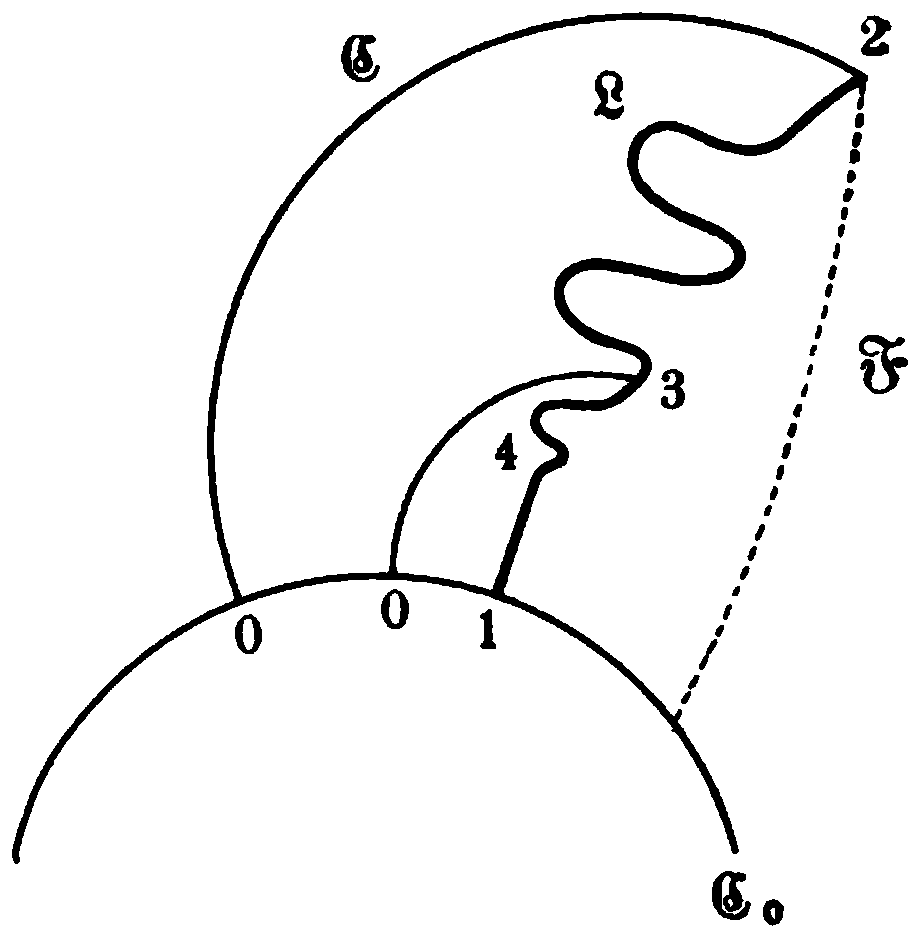
\includegraphics[width=\linewidth,height=42mm,keepaspectratio]{fig_assets/fig17_p0169_src_clean_x8.png}\par\vspace{1mm}
\end{minipage}
\end{center}

Die Extremalen sind Kreise (Fig.~17) und liegen nach \S~34 zum Kreise $\mathfrak{C}_0$ transversal, wenn sie ihn senkrecht schneiden. Da nun jeder Punkt 3 mit dem Kreise $\mathfrak{C}_0$ durch einen zu diesem orthogonalen Kreisbogen 03 gegebener Länge verbunden werden kann, sobald diese Länge die kürzeste gerade Verbindungsstrecke zwischen dem Punkte und $\mathfrak{C}_0$ übersteigt, so ist die \textsc{Weierstrass}'sche Construction längs irgend eines Bogens $\Omega$ oder 12 von der vorgeschriebenen Länge immer in der Weise möglich, dass der Bogen 03 dem längs der Curve $\Omega$ gemessenen Bogen 13 gleich ist; dabei können die Kreisbögen 03 so gewählt werden, dass ein den Kreis $\mathfrak{C}_0$ in bestimmter Richtung $\mathfrak{R}$ umlaufender Punkt an jeder Stelle 0 nach der concaven Seite des Bogens 03 geht. Diese Construction ist jedoch nur für ein
% src-pdfpage=0170
% src-break=0170
Stück 42 des Bogens $\Omega$ durchzuführen, wenn dieser mit der zum Kreise $\mathfrak{C}_0$ normalen geraden Strecke 14 beginnt, im Punkte 4 aber die Gerade 14 verlässt; dann ist die Strecke 14 die Grenze der Bögen 03, wenn man 3 und 4 zusammenrücken lässt, so dass
\begin{equation}\tag{29}
\left.\overline{J}_{03}+J_{32}\right|^{\tau_4}=J_{12},\quad
\left.\overline{K}_{03}+K_{32}\right|^{\tau_4}=K_{12}
\end{equation}
gesetzt werden kann. Da ferner, wenn der Punkt 3 in die Lage 2 rückt, die Grenzlage des Bogens 03 der Bogen $\mathfrak{C}$ oder 02 ist, mit welchem $\Omega$ verglichen wird, also die Gleichung
\[
\lim \overline{J}_{03}=\overline{J}_{02}
\]
gilt, so ist nach (29)
\[
\left.\overline{J}_{03}+J_{32}\right|_{\tau_4}^{\tau_2}=\int_{\tau_4}^{\tau_2}\mathfrak{E}\,d\tau=\overline{J}_{02}-J_{12},
\]
woraus, da $\mathfrak{E}$ ein festes Vorzeichen hat, das Extremum folgt, so lange die \textsc{Jacobi}'sche Bedingung erfüllt ist.

Um zu erkennen, in welchem Umfange dies der Fall ist, nehmen wir an, es sei
\[
x_0^2+y_0^2=r^2
\]
die Gleichung des Kreises $\mathfrak{C}_0$; ist $b$ die in der Richtung $\mathfrak{R}$ wachsende Bogenlänge, so sind
\[
\alpha=x_0+a\frac{dx_0}{db},\quad \beta=y_0+a\frac{dy_0}{db}
\]
die Coordinaten des Centrums eines Bogens 03 vom Radius $|a|$; bei der Bedeutung von $\mathfrak{R}$ ist $a$ positiv. Nach der in \S~37 benutzten Darstellungsweise kann der Kreisbogen 03, indem man den Coordinatenanfangspunkt durch den Punkt 0 ersetzt, durch folgende Gleichungen dargestellt werden:
\[
\begin{aligned}
x-x_0&=(\alpha-x_0)-(\alpha-x_0)\cos t-(\beta-y_0)\sin t,\\
y-y_0&=(\beta-y_0)+(\alpha-x_0)\sin t-(\beta-y_0)\cos t,
\end{aligned}
\]
oder, wenn man setzt
\[
\xi(t,a,b)=x_0+a\frac{dx_0}{db}-a\frac{dx_0}{db}\cos t-a\frac{dy_0}{db}\sin t,
\]
\[
\eta(t,a,b)=y_0+a\frac{dy_0}{db}+a\frac{dx_0}{db}\sin t-a\frac{dy_0}{db}\cos t,
\]
durch die Gleichungen
\[
x=\xi(t,a,b),\quad y=\eta(t,a,b).
\]
Offenbar ist $t=0$ im Punkte 0; also hat man
\[
\overline{K}_{03}=at=\omega(t,a,b),
\]
% src-pdfpage=0171
% src-break=0171
\begingroup
\setlength{\arraycolsep}{1pt}
\[
\Delta=\frac{\partial(\xi,\eta,\omega)}{\partial(t,a,b)}=
\begin{vmatrix}
 a\dfrac{dx_0}{db}\sin t-a\dfrac{dy_0}{db}\cos t & a\dfrac{dx_0}{db}\cos t+a\dfrac{dy_0}{db}\sin t & a\\[1.0ex]
 \dfrac{dx_0}{db}(1-\cos t)-\dfrac{dy_0}{db}\sin t & \dfrac{dy_0}{db}(1-\cos t)+\dfrac{dx_0}{db}\sin t & t\\[1.0ex]
 \dfrac{dx_0}{db}+a\dfrac{d^2x_0}{db^2}(1-\cos t)-a\dfrac{d^2y_0}{db^2}\sin t & \dfrac{dy_0}{db}+a\dfrac{d^2y_0}{db^2}(1-\cos t)+a\dfrac{d^2x_0}{db^2}\sin t & 0
\end{vmatrix}.
\]
\endgroup
Wenn nun für den betrachteten Bogen 03 die Gleichungen
\begin{equation}\tag{30}
\frac{dy_0}{db}=0,\quad \frac{dx_0}{db}=1
\end{equation}
bestehen, so ergiebt die Identität
\[
\frac{dy_0}{db}\frac{d^2y_0}{db^2}+\frac{dx_0}{db}\frac{d^2x_0}{db^2}=0
\]
sofort die Folgerung
\[
\frac{d^2x_0}{db^2}=0;
\]
man erhält daher
\[
\Delta=-a(\sin t-t\cos t)+a^2\frac{d^2y_0}{db^2}\begin{vmatrix}
\sin t&\cos t&1\\
1-\cos t&\sin t&t\\
-\sin t&1-\cos t&0
\end{vmatrix},
\]
und mit der Bezeichnung
\[
\varphi(t)=\sin t-t\cos t
\]
ergiebt sich
\[
\Delta=-a\varphi(t)+4a^2\frac{d^2y_0}{db^2}\sin\frac{t}{2}\,\varphi\left(\frac{t}{2}\right).
\]
Ferner gelten offenbar längs des Kreises $\mathfrak{C}_0$ die Gleichungen
\[
x_0=r\cos\frac{b}{r},\quad y_0=r\sin\frac{b}{r};
\]
und wenn für den Punkt 0 die Annahme
\[
b=\frac{3r\pi}{2}
\]
gemacht wird, so bestehen die Gleichungen (30) und damit auch die folgenden:
% src-pdfpage=0172
% src-break=0172
\[
\frac{d^2y_0}{db^2}=-\frac{1}{r}\sin\frac{b}{r}=\frac{1}{r},
\]
\[
\Delta=-\frac{a}{r}\left\{r\varphi(t)-4a\sin\frac{t}{2}\,\varphi\left(\frac{t}{2}\right)\right\}.
\]
So lange daher die Kreisbögen 03 in Theilen des Radius $a$ gemessen die kleinste Wurzel der Gleichung
\[
r\varphi(t)-4a\sin\frac{t}{2}\,\varphi\left(\frac{t}{2}\right)=0
\]
nicht erreichen, liefert der Bogen 02 wirklich ein Extremum der Fläche, die von ihm, dem Kreise $\mathfrak{C}_0$ und einer festen, diesen mit 2 verbindenden Linie umschlossen wird.

Man sieht leicht, dass dies Resultat gültig bleibt, wenn $\mathfrak{C}_0$ eine beliebige reguläre Curve ist, und $r$ ihr Krümmungsradius in dem Punkte, in welchem sie von dem Kreisbogen 03 orthogonal geschnitten wird.

\noindent\textbf{Aufgabe XI (\S~38).} Die Stabilität eines schweren Fadens zu untersuchen, wenn der eine Endpunkt fest, der andere auf einer gegebenen Curve beweglich ist.

Wir gehen von der folgenden allgemeinen Bemerkung aus. Eine zweifach unendliche Schar von Extremalen, welche durch einen Punkt 0 gehen, oder die Curve $\mathfrak{C}_0$ transversal schneiden, sei durch die Gleichungen
\[
x=\xi(t,a,b,c),\quad y=\eta(t,a,b,c),
\]
\[
\overline{K}_{03}=\omega=\omega(t,a,b,c),\quad g(a,b,c)=0
\]
gegeben, $g_c$ sei von Null verschieden; dann hat die Grösse $\Delta$ folgende Form:
\begingroup
\setlength{\arraycolsep}{1pt}
\[
\Delta=\frac{\partial(\xi,\eta,\omega)}{\partial(t,a,b)}=
\begin{vmatrix}
\xi_t&\xi_a+\xi_c\dfrac{\partial c}{\partial a}&\xi_b+\xi_c\dfrac{\partial c}{\partial b}\\[1.0ex]
\eta_t&\eta_a+\eta_c\dfrac{\partial c}{\partial a}&\eta_b+\eta_c\dfrac{\partial c}{\partial b}\\[1.0ex]
\omega_t&\omega_a+\omega_c\dfrac{\partial c}{\partial a}&\omega_b+\omega_c\dfrac{\partial c}{\partial b}
\end{vmatrix},
\]
und da offenbar die Gleichungen
\[
g_a+g_c\frac{\partial c}{\partial a}=g_b+g_c\frac{\partial c}{\partial b}=0
\]
gelten, so folgt
% src-pdfpage=0173
% src-break=0173
\[
\Delta g_c^2=\begin{vmatrix}
\xi_t&\xi_ag_c-\xi_cg_a&\xi_bg_c-\xi_cg_b\\
\eta_t&\eta_ag_c-\eta_cg_a&\eta_bg_c-\eta_cg_b\\
\omega_t&\omega_ag_c-\omega_cg_a&\omega_bg_c-\omega_cg_b
\end{vmatrix}
=g_c\begin{vmatrix}
\xi_t&\xi_a&\xi_b&\xi_c\\
\eta_t&\eta_a&\eta_b&\eta_c\\
\omega_t&\omega_a&\omega_b&\omega_c\\
0&g_a&g_b&g_c
\end{vmatrix},
\]
\endgroup
so dass $g_c\Delta$ der rechts stehenden Determinante vierter Ordnung gleich ist.

Die gegebene Curve $\mathfrak{C}_0$ habe nun die Gleichung
\[
y_0=f(x_0);
\]
sie sei an der betrachteten Stelle nicht horizontal, $f'(x_0)$ also von Null verschieden. Die Extremalen, für welche
\[
y+\lambda=a\Cof\frac{x-b}{a},\quad p=\Sin\frac{x-b}{a}
\]
ist, müssen von $\mathfrak{C}_0$ im Punkte 0 senkrecht geschnitten werden, wenn 0 der bewegliche Endpunkt des Fadens ist; man hat daher die Gleichungen
\begin{equation}\tag{31}
\begin{aligned}
y_0+\lambda&=a\Cof\frac{x_0-b}{a},\\
1+f'(x_0)p_0&=1+f'(x_0)\Sin\frac{x_0-b}{a}=0,
\end{aligned}
\end{equation}
und die gesammte Schar der transversal schneidenden Extremalen wird, indem man $-x=t$ setzt und durch $\omega$ die vom Punkte 0 aus im Sinne abnehmender $x$ gemessene Länge bezeichnet, durch folgende Gleichungen definirt:
\[
x=-t,\quad y=f(x_0)+a\left(\Cof\frac{x-b}{a}-\Cof\frac{x_0-b}{a}\right),
\]
\[
\omega=-a\left(\Sin\frac{x-b}{a}-\Sin\frac{x_0-b}{a}\right),\quad
0=1+f'(x_0)\Sin\frac{x_0-b}{a}.
\]
Die Grösse $-\Delta$, multiplicirt mit dem Analogon der oben durch $g_c$ bezeichneten Grösse, ist daher die Functionaldeterminante der rechten Seiten der letzten drei Gleichungen nach $a,b,x_0$; setzt man
\[
\frac{x-b}{a}=u,
\quad
\frac{x_0-b}{a}=u_0,
\]
so findet man auf Grund der Additionsformeln der Functionen $\Sin,\Cof$ unmittelbar
\[
\Delta=-\Phi(u)+\frac{1}{a}\Ctg^2u_0\,\Phi'(u)\left[f''(x_0)\Sin u_0-\frac{1}{a}\Ctg u_0\right]^{-1},
\]
wobei gesetzt ist
% src-pdfpage=0174
% src-break=0174
\[
\Phi(u)=2-2\Cof(u-u_0)+(u-u_0)\Sin(u-u_0).
\]
Für diese Function gelten die Gleichungen
\[
\Phi(u_0)=\Phi'(u_0)=0,\quad \Phi''(u)=(u-u_0)\Sin(u-u_0)
\]
\[
\Phi(u)\Phi''(u)-[\Phi'(u)]^2=[\Phi(u)]^2\frac{d}{du}\left[\frac{\Phi'(u)}{\Phi(u)}\right]
= -[u-u_0-\Sin(u-u_0)]^2,
\]
\[
\frac{\Phi'(u)}{\Phi(u)}=\frac{u-u_0-\Tg(u-u_0)}{(u-u_0)\Tg(u-u_0)-2+[2:\Cof(u-u_0)]},
\]
aus welchen unmittelbar folgt, dass für $u>u_0$ die Grössen $\Phi(u)$ und $\Phi'(u)$ stets positiv sind, der Quotient $\Phi'(u):\Phi(u)$ aber, wenn man $u$ von $u_0$ ausgehen und positiv unendlich werden lässt, das Intervall von $+\infty$ bis $+1$ beständig abnehmend durchläuft.

Fasst man nun nur solche Gleichgewichtslagen ins Auge, für welche die \textsc{Legendre}'sche Bedingung des Maximums der Schwerpunktsordinate erfüllt ist, so müssen die betrachteten Extremalen nach unten convex sein, mithin, da $+y$ die Richtung der Schwere ist, $a<0$. Die Gleichung
\begin{equation}\tag{32}
\Delta=0,
\quad
\frac{\Phi'(u)}{\Phi(u)}=\Tg u_0\left[\frac{a f''(x_0)\Sin^2u_0}{\Cof u_0}-1\right]
\end{equation}
hat daher, wenn $\Sin u_0$ und damit $\Tg u_0$ ebenso wie $f''(x_0)$ positiv ist, keine Wurzel oberhalb des Werthes $u_0$. Dasselbe gilt aber auch, da die Gleichung geschrieben werden kann
\[
\Cof u_0\left[\Ctg u_0\frac{\Phi'(u)}{\Phi(u)}+1\right]=a f''(x_0)\Sin^2u_0,
\]
wenn $\Sin u_0$ negativ, $f''(x_0)$ nicht positiv ist; denn dann ist
\[
\Ctg u_0<-1,
\]
die linke Seite der letzten Gleichung also für $u>u_0$ sicher negativ, die rechte dagegen positiv oder Null. Nun haben nach (31) die Grössen $\Sin u_0$ und $f'(x_0)$ entgegengesetzte Vorzeichen; in den beiden betrachteten Fällen haben also $f'(x_0)$ und $f''(x_0)$ entgegengesetzte Vorzeichen, so dass die Richtung abnehmender $x$ oder, da $a$ negativ ist, wachsender $u$ nach der convexen Seite der Curve $\mathfrak{C}_0$ hinweist. Die \textsc{Jacobi}'sche Bedingung für die Stabilität des Gleichgewichts ist also immer erfüllt, wenn der Faden im Punkte 0 nach der convexen Seite der Curve $\mathfrak{C}_0$ hingeht, oder diese im Punkte 0 die Krümmung Null hat, z.~B. eine Gerade ist. Wenn in einem dieser Fälle die \textsc{Weierstrass}'sche
% src-pdfpage=0175
% src-break=0175
Construction möglich ist, so liegen alle Bögen 03 im Inneren des Feldes, und die Stabilität ist für ein beliebig langes Stück des Fadens gesichert.

Haben $f''(x_0)$ und $f'(x_0)$ dasselbe Zeichen, so dass der Faden, für welchen $u>u_0$ sei, nach der concaven Seite der Curve $\mathfrak{C}_0$ hingeht, so hat die Gleichung (32) für $u>u_0$ eine einzige Wurzel $\bar u$, sobald die Ungleichung
\[
\Tg u_0\left[\frac{a f''(x_0)\Sin^2u_0}{\Cof u_0}-1\right]>1
\]
besteht. Sieht man daher die Richtung der Curve $\mathfrak{C}_0$ und die Gestalt des Fadens, d.~h. die Grössen $a$ und $u_0$ als fest an, und lässt die Krümmung der Curve $\mathfrak{C}_0$ variiren, so tritt eine Wurzel $\bar u$ auf, sobald der absolute Werth der Krümmung eine gewisse Grenze erreicht hat. Wächst derselbe über alle Grenzen, so nähert sich $\bar u$ beständig abnehmend der Grenze $u_0$ an, d.~h. das Stück des Fadens, für welches die \textsc{Jacobi}'sche Bedingung erfüllt ist, wird unendlich klein.

Um nun die \textsc{Weierstrass}'sche Construction zu discutiren, suchen wir eine Kettenlinie, welche im Punkte 0 die feste, weder horizontal noch vertical liegende Gerade $T$ berührt, und ausserdem den Punkt 1 enthält, der nicht auf derselben Verticalen wie 0 liegt. Die Gleichung der Geraden $T$ kann man schreiben:
\[
y-y_0=(x-x_0)\Sin u_0;
\]
der Werth $u_0$ ist dann eindeutig bestimmt, da die Function $\Sin$ bei wachsendem Argument alle Werthe von $-\infty$ bis $+\infty$ wachsend durchläuft. Die sämmtlichen im Punkte 0 die Gerade $T$ berührenden Kettenlinien werden durch die Gleichungen
\begin{equation}\tag{33}
y-y_0=a(\Cof u-\Cof u_0),\quad x=x_0+a(u-u_0)
\end{equation}
dargestellt, in welchen $u$ ein Parameter ist. Sehen wir $a$ als veränderlich, $x$ als fest an, so hat man
\[
\frac{\partial y}{\partial a}=\Cof u+a\Sin u\frac{\partial u}{\partial a}-\Cof u_0
=\Cof u-(u-u_0)\Sin u-\Cof u_0;
\]
die Ableitung der rechten Seite nach $u$ ist $(u_0-u)\Cof u$, hat also das Vorzeichen der Differenz $u_0-u$, die Grösse selbst verschwindet für $u=u_0$, ist also negativ, so lange $u$ endlich und von $u_0$ verschieden bleibt. Für unendlich kleine Werthe von $a$ erhält man nun, je nachdem $a$ positiv oder negativ ist,
% src-pdfpage=0176
% src-break=0176
\[
\Cof u=+\infty,\quad y=\pm\infty.
\]
Da ferner die erste Gleichung (33) geschrieben werden kann
\[
y-y_0=(x-x_0)\Sin u_0+(x-x_0)[u-u_0]_1,
\]
wobei die Coëfficienten der letzten Reihe von $a$ unabhängig sind, so folgt für $a=\pm\infty$ die Gleichung
\[
y=y_0+(x-x_0)\Sin u_0.
\]
Die Grösse $y$ geht also von diesem Werthe aus abnehmend bis $-\infty$, dann ebenso von $+\infty$ bis zu diesem Werthe zurück, wenn man $a$ von $-\infty$ bis $+\infty$ wachsen lässt und für $x$ einen festen Werth, etwa $x_1$, festhält. Für einen einzigen, bestimmten Werth von $a$ erhält man daher, wenn $x_1-x_0$ von Null verschieden ist, $y=y_1$, womit die gesuchte Curve gefunden und als eindeutig bestimmt nachgewiesen ist. Sie ist nach unten convex ($a<0$), wenn der Punkt $(x_1,y_1)$ oberhalb der Geraden $T$ liegt, d.~h. wenn
\[
y_1<y_0+(x_1-x_0)\Sin u_0.
\]
Jetzt beschränken wir uns auf den Fall $f'(x_0)>0$, in welchem die Kettenlinie, in der Richtung abnehmender $x$ verfolgt, von der Curve $\mathfrak{C}_0$ aus sich zunächst senkt. Nähert sich (Fig.~18) dann der Punkt 3 auf der Curve $\Omega$ der Lage 1, d.~h. ihrem Schnittpunkt mit $\mathfrak{C}_0$, so wird der längs der Curve $\Omega$ gemessene Abstand 13 oder $K_{13}$ unendlich klein. Verbindet man daher den Punkt 3 mit einem festen auf der Curve $\mathfrak{C}_0$ und tiefer als der Punkt 1 liegenden Punkte 4 durch eine zur Curve $\mathfrak{C}_0$ rechtwinkelige Extremale, so ist diese nach unten convex, da, sobald der Bogen 13 hinreichend klein ist, der Punkt 3 oberhalb der Normale des Punktes 4 liegt, und die Länge des Extremalenbogens 34, welche wir $\mathfrak{R}_{34}$ nennen, bleibt oberhalb einer positiven Grenze, wenn $K_{13}$ unendlich abnimmt. Daraus folgt, dass man einen von 1 beginnenden Theil $\Omega_1$ von der Curve $\Omega$ abschneiden kann, für welchen die Ungleichung
\begin{equation}\tag{34}
K_{13}<\mathfrak{R}_{34}
\end{equation}
gilt, sobald 3 ein Punkt des Bogens $\Omega_1$ ist. Ist ferner 35 die durch 3 gehende Normale der Curve $\mathfrak{C}_0$, und lässt man längs der

\begin{center}
\begin{minipage}{0.48\linewidth}\centering
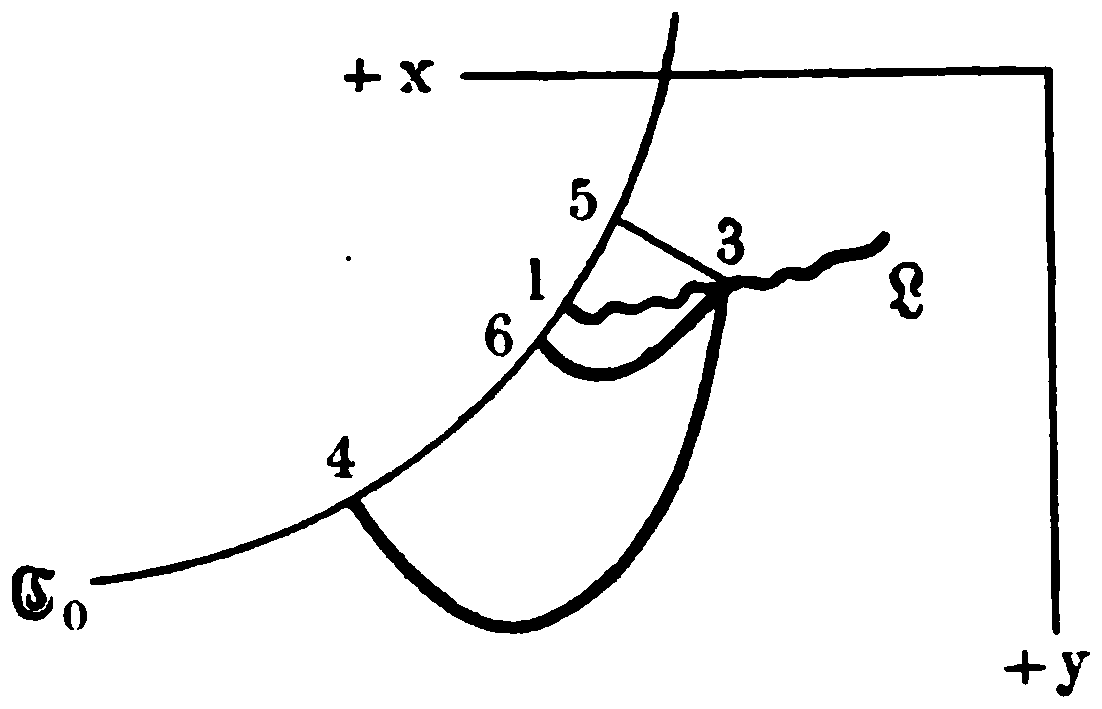
\includegraphics[width=\linewidth,height=35mm,keepaspectratio]{fig_assets/fig18_p0176_src_clean_x8.png}\par\vspace{1mm}
\end{minipage}
\end{center}

% src-pdfpage=0177
% src-break=0177
Curve $\mathfrak{C}_0$ den Punkt 6 von 4 bis 5 laufen, so liegt derselbe niemals vertical über oder unter 3 und seine Normale läuft stets unter dem Punkte 3 durch. Es kann daher stets eine die Curve $\mathfrak{C}_0$ senkrecht schneidende nach unten convexe Extremale 36 construirt werden, für deren Länge $\mathfrak{R}_{36}$, wenn $\mathfrak{R}_{35}$ der geradlinige Abstand 35 ist, die Ungleichung
\[
\mathfrak{R}_{36}>\mathfrak{R}_{35}
\]
gilt, und $\mathfrak{R}_{36}-\mathfrak{R}_{35}$ kann beliebig klein werden. Da nun offenbar
\[
K_{13}\geq \mathfrak{R}_{35},
\]
so ergiebt sich der Ungleichung (34) zufolge für mindestens eine Lage des Punktes 6
\[
K_{13}=\mathfrak{R}_{36},
\]
womit die \textsc{Weierstrass}'sche Construction zunächst für den Bogen $\Omega_1$ durchgeführt ist. Für den Rest der Curve $\Omega$ folgt ihre Möglichkeit aus \S~38, wenn man in der dort gegebenen Weise variirt; denn die Grösse $\Delta$ verschwindet hier nicht mehr, so lange die \textsc{Jacobi}'sche Bedingung für die Kettenlinie 02 erfüllt ist. Der Fall, dass die Curve $\Omega$ mit einer zu $\mathfrak{C}_0$ normalen geraden Strecke beginnt, kann ebenso leicht wie oben bei der Aufgabe IX erledigt werden.

% machine-unit: Kneser_LVR_DE_p0177low_p0192 §§40-42
% appended in continuation package p0177-p0192; §43 excluded.

% src-pdfpage=0177
% src-break=0177-partial-lower
\begin{center}
{\large \S~40.}
\end{center}

Die folgende Entwickelung gilt, gleichviel ob die Extremalen des Feldes einen festen Punkt 0 gemein haben, oder eine feste Curve $\mathfrak{C}_0$ in dem veränderlichen Punkte 0 transversal schneiden.

Bewegt man sich längs des Bogens $\mathfrak{C}$ von dem auf ihm liegenden Punkte 0 aus, so möge die Grösse $\Delta$ zum ersten Male verschwinden in einem Punkte 1 und für ein solches Argument $t=t_1$, dass an der Stelle $(t_1,a_0,b_0)$ die Functionen $\xi,\eta,\omega$ regulär sind und die Grössen $\xi_t,\eta_t$ nicht beide verschwinden. Dann heisst der Punkt 1 im ersten der oben unterschiedenen Fälle zum Punkte 0 conjugirt, im zweiten der extremale Brennpunkt der Curve $\mathfrak{C}_0$ für die vorliegende Aufgabe, und man hat die charakteristische Eigenschaft
\begin{equation}\tag{35}
\Delta(t_1,a_0,b_0)=0.
\end{equation}
Die in \S~36 an die Gleichungen (10), (11) geknüpfte Entwickelung giebt dann Anleitung, eine Curve 01 herzustellen, längs
% src-pdfpage=0178
% src-break=0178
 deren die \textsc{Weierstrass}'sche Construction möglich ist, die Grösse $\mathfrak{E}$ aber überall verschwindet, so dass sich die Gleichungen
\begin{equation}\tag{36}
\bar J_{01}=J_{01},\quad \bar K_{01}=K_{01}
\end{equation}
ergeben, und damit das Extremum aufhört. Zu diesem Zwecke werde zunächst $t$ als Function von $a$ und $b$ durch die Gleichung
\begin{equation}\tag{37}
\Delta(t,a,b)=0
\end{equation}
definirt; nehmen wir an, es sei
\[
\Delta_t(t_1,a_0,b_0)\gtrless 0,
\]
so ergiebt sich mit Rücksicht auf die Gleichung (35) für $t$ ein Ausdruck
\[
t=t_1+[a-a_0,b-b_0]_1.
\]
Wir setzen ferner die Differentialgleichung
\[
\left|\begin{array}{cc}
\xi_tdt+\xi_a da+\xi_b db&\eta_tdt+\eta_a da+\eta_b db\\[.6ex]
\xi_t&\eta_t
\end{array}\right|=0
\]
oder
\begin{equation}\tag{38}
(\xi_t\eta_a-\xi_a\eta_t)\,da+(\xi_t\eta_b-\xi_b\eta_t)\,db=0
\end{equation}
an, und substituiren für $t$ den erhaltenen Ausdruck; dann sind die Factoren von $da$ und $db$ Potenzreihen der Argumente $a-a_0$, $b-b_0$, welche für $a=a_0$, $b=b_0$ nicht beide verschwinden, wenn wir die Voraussetzung einführen, dass die Determinanten zweiter Ordnung in der Matrix
\begin{equation}\tag{39}
\begin{array}{ccc}
\xi_t&\xi_a&\xi_b\\
\eta_t&\eta_a&\eta_b
\end{array}
\end{equation}
für das Werthsystem $t=t_1$, $a=a_0$, $b=b_0$ nicht sämmtlich verschwinden. Hätten nämlich jene beiden Factoren den Werth Null, so würde dasselbe für die dritte Determinante der Matrix folgen, da $\xi_t$ und $\eta_t$ nicht beide verschwinden. Die Gleichung (38) ergiebt also, wenn $a_0$ und $b_0$ zusammengehörige Werthe sein sollen, eine Beziehung von einer der Formen
\[
b-b_0=[a-a_0]_1,\quad a-a_0=[b-b_0]_1.
\]
Gilt z.~B. die erste Gleichung, und substituirt man die erhaltenen Werthe von $b$ und $t$ in die Gleichungen
\begin{equation}\tag{40}
x=\xi(t,a,b),\quad y=\eta(t,a,b),
\end{equation}
so erscheinen $x$ und $y$ in der Form von Ausdrücken $[a-a_0]_0$, und man hat für $a=a_0$ speciell
\[
x=x_1,\quad y=y_1.
\]
Die Gleichungen (40) stellen also eine den Punkt 1 enthaltende Curve $\mathfrak{C}$ dar, welche in der Nähe dieses Punktes, abgesehen von
% src-pdfpage=0179
% src-break=0179
ihm selbst, regulär ist. Sollte der Punkt 1 ein Rückkehrpunkt sein, so hätte man für ihn die Gleichungen
\[
\xi_tdt+\xi_a da+\xi_b db=0,\quad \eta_tdt+\eta_a da+\eta_b db=0;
\]
da nun die Gleichung
\[
\Delta_tdt+\Delta_a da+\Delta_b db=0
\]
gilt und eine der Grössen $\dfrac{db}{da}$ und $\dfrac{da}{db}$ von Null verschieden ist, so würde folgen
\begin{equation}\tag{41}
\frac{\partial(\xi,\eta,\Delta)}{\partial(t,a,b)}=0.
\end{equation}
Besteht also diese Gleichung für $t=t_1$, $a=a_0$, $b=b_0$ nicht, so hat die Curve $\mathfrak{C}$ im Punkte 1 keinen Rückkehrpunkt.

Aus der Gleichung (38) folgt nun, da $\xi_t$ und $\eta_t$ nicht zugleich verschwinden, dass man setzen kann:
\begin{equation}\tag{42}
\xi_tdt+\xi_a da+\xi_b db=m\xi_tdt,\quad
\eta_tdt+\eta_a da+\eta_b db=m\eta_tdt;
\end{equation}
die Curve $\mathfrak{C}$ wird also in jedem Punkte von der zu demselben Werthsystem $(a,b)$ gehörigen Extremale (40) berührt, und ist die Enveloppe einer gewissen einfach unendlichen Schar dieser Curven.

Aus den Gleichungen (42) ergiebt sich auf Grund der Gleichung (37) und der betreffs des Systemes (39) eingeführten Voraussetzung
\[
\omega_tdt+\omega_a da+\omega_b db=m\omega_tdt,
\]
oder, da offenbar
\[
\omega_t=G(\xi,\eta,\xi_t,\eta_t)
\]
gesetzt werden kann,
\[
\omega_tdt+\omega_a da+\omega_b db=mG(\xi,\eta,\xi_t,\eta_t)dt.
\]
Wenn nun $mdt$ positiv ist, so kann man hieraus wegen der Homogeneität der Function $G$ und der Gleichungen (42) schliessen
\[
\omega_tdt+\omega_a da+\omega_b db
=G(\xi,\eta,\xi_tdt+\xi_a da+\xi_b db,\eta_tdt+\eta_a da+\eta_b db).
\]
Die Differentiale $dt,da,db$ beziehen sich alle auf den Fortgang längs der Curve $\mathfrak{C}$; bezeichnet man im Uebrigen die diesem Fortgang entsprechenden Incremente durch $D$, so kann man die letzte und die Gleichungen (42) schreiben
\[
Dx=m\xi_tdt,
\quad Dy=m\eta_tdt,
\quad D\omega=G(\xi,\eta,Dx,Dy).
\]
% src-pdfpage=0180
% src-break=0180
Somit folgt, wenn das ungestrichene Integralzeichen $K$ auf die Curve $\mathfrak{C}$ bezogen wird und 3 ein Punkt derselben ist (Fig.~19), aus der Gleichung
\[
DK_{31}=-G(x,y,Dx,Dy)
\]
für $mdt>0$ das Resultat
\begin{equation}\tag{43}
D\omega+DK_{31}=D(\bar K_{03}+K_{31})=0,
\end{equation}
wobei das gestrichene $K$ sich auf diejenige Extremale 03 bezieht, welche durch das zum Punkte 3 gehörige Werthsystem $(a,b)$ definirt wird. Diese Extremalen liefern also für die Curve $\mathfrak{C}$ die \textsc{Weierstrass}'sche Construction, und die Grösse
\[
\mathfrak{E}(x,y,x',y',Dx,Dy)=\mathfrak{E}(x,y,\xi_t,\eta_t,Dx,Dy)
\]
verschwindet dabei in ordentlicher Weise, wenn $mdt$ positiv ist.

\begin{center}
\textbf{Fig. 19.}\par\vspace{1mm}
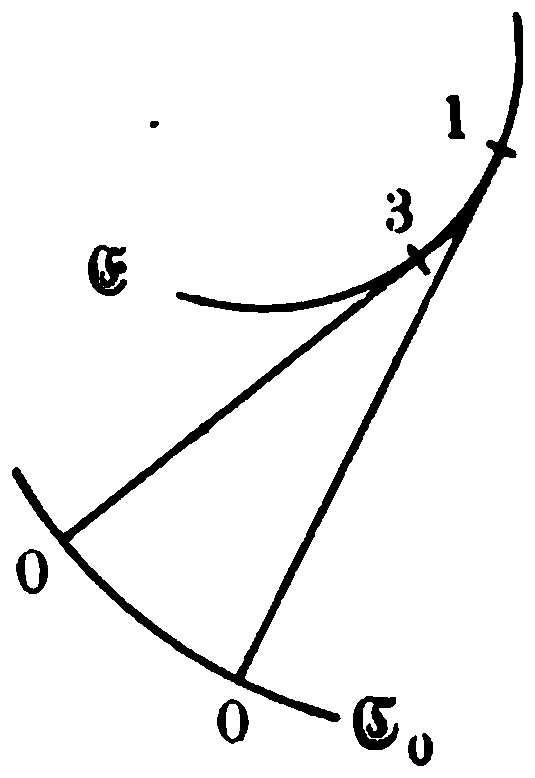
\includegraphics[width=.34\linewidth,height=55mm,keepaspectratio]{fig_assets/fig19_p0180_src_clean_x8.png}
\end{center}

Um hieraus die Gleichungen (36) erschliessen zu können, muss das Zeichen $D$ den Fortgang auf der Curve $\mathfrak{C}$ in der Richtung zum Punkte 1 hin bedeuten. Diese Richtung kann mit der Richtung wachsender $t$ auf der im Punkte 3 berührenden Extremale übereinstimmen oder nicht. Letzterer Fall wird dann immer eintreten, wenn die Curve $\mathfrak{C}$ im Punkte 1 einen Rückkehrpunkt hat, von welchem beide Zweige der Curve in der Richtung der mit wachsendem $t$ durchlaufenen Curve $\mathfrak{C}$ ausgehen; haben die beiden Zweige die entgegengesetzte Richtung oder ist gar kein Rückkehrpunkt vorhanden, so stimmt in mindestens einer der beiden Hälften, in welche die Curve $\mathfrak{C}$ in der Umgebung des Punktes 1 durch diesen zerlegt wird, die Richtung der Curve $\mathfrak{C}$ nach dem Punkte 1 hin überein mit der Richtung wachsender Werthe von $t$ auf der Extremalen 03; diese Hälfte werde durch $\mathfrak{C}_1$ bezeichnet. Letztere Richtung wird durch das Werthepaar
\[
x'=\xi_t,
\quad y'=\eta_t
\]
definirt; auf der Hälfte $\mathfrak{C}_1$ unterscheiden sich also $Dx$ von $\xi_t$ und $Dy$ von $\eta_t$ um einen positiven Factor, so dass $mdt$ positiv ist, und demnach die bezeichnete Grösse $\mathfrak{E}$ verschwindet. Ein solcher Bogen $\mathfrak{C}_1$ ist also jedenfalls dann vorhanden, wenn die Gleichung (41) nicht gilt und damit ein Rückkehrpunkt ausgeschlossen ist.

Es sei nun 3 irgend ein beliebig nahe bei 1 liegender Punkt des Bogens $\mathfrak{C}_1$; dann bildet die oben construirte Extremale 03
% src-pdfpage=0181
% src-break=0181
mit dem Bogen 31 der Curve $\mathfrak{C}_1$ einen zusammenhängenden Linienzug mit stetig veränderlicher Tangente, welcher beliebig wenig von dem der Curve $\mathfrak{C}$ angehörigen Bogen 01 abweicht, und zwar so, dass in benachbarten Punkten beider Linienzüge auch die Tangenten nur wenig verschieden sind. Dabei hat man die Gleichung
\[
d(\bar J_{03}+J_{31})=\mathfrak{E}(x,y,x',y',Dx,Dy)=0;
\]
denn die Ausdrücke für die partiellen Differentialquotienten von $\bar J_{03}$ und $J_{31}$, welche oben abgeleitet sind, bleiben auch in der Umgebung der Stelle $(t_1,a_0,b_0)$ gültig, weil die bezeichneten Integrale auch hier reguläre Functionen von $t,a,b$ sind. Aus der erhaltenen und der für die \textsc{Weierstrass}'sche Construction charakteristischen Gleichung (43) folgt
\[
\bar J_{03}+J_{31}=\bar J_{01},
\quad \bar K_{03}+K_{31}=\bar K_{01}.
\]
Der Bogen 01 der Curve $\mathfrak{C}$ liefert also nicht mehr ein Extremum des Integrals $J$ im Vergleich zu allen Curven, welche denselben Werth des Integrals $K$ ergeben; vielmehr hört, wegen der angegebenen Eigenschaften des Linienzuges 031, schon das schwache Extremum im Punkte 1 auf.

\noindent\textbf{Beispiel. Aufgabe IX} werde in folgender Weise specialisirt. Von einem gegebenen Punkte des einen Schenkels eines Winkels auf der convexen Seite nach dem anderen Schenkel eine Linie gegebener Länge zu ziehen, welche mit den Schenkeln eine grösstmögliche Fläche umschliesst.

Der zweite Schenkel sei die Linie $y=0$; die extrem zu machende Fläche unterscheidet sich von dem Integral $\int yx' dt$ nur um die constante Dreiecksfläche, welche das vom gegebenen Punkte auf den zweiten Schenkel gefällte Loth von dem Winkel abschneidet. Die Extremalen, welche die Linie $y=0$ transversal schneiden, stehen auf ihr (\S~34) senkrecht und sind Kreise, können daher durch die Gleichungen
\begin{equation}\tag{44}
x=a+b\cos t,
\quad y=b\sin t
\end{equation}
dargestellt werden; für den Punkt 0 ist immer $t=0$, so dass
\[
\bar K_{03}=\omega(t,a,b)=bt.
\]
Es ergiebt sich hieraus
\[
\Delta=\begin{vmatrix}
-b\sin t&b\cos t&b\\
1&0&0\\
\cos t&\sin t&t
\end{vmatrix}=b(\sin t-t\cos t);
\]
% src-pdfpage=0182
% src-break=0182
der extremale Brennpunkt der Geraden $y=0$ auf jedem zu ihr orthogonalen Kreise ist also durch die kleinste Wurzel der Gleichung
\[
\tg t=t
\]
definirt, welche durch $t_1$ bezeichnet werde und annähernd den Werth
\[
t_1=\frac{257\frac{1}{2}}{360}\cdot 2\pi
\]
hat, d.~h. dem Winkel $257\frac{1}{2}^{\circ}$ entspricht. Die Gleichung (38), welche den die Curve $\mathfrak{C}$ definirenden Zusammenhang liefert, wird einfach
\[
b\,db+b\cos t_1\,da=0,
\quad db+\cos t_1\,da=0.
\]
Eine solche Beziehung zwischen $a$ und $b$ sondert aus der zweifach unendlichen Schar von Kreisen (44) eine einfach unendliche von solchen aus, welche zwei feste Gerade berühren; ist $\alpha$ der concave Winkel derselben, so ist
\[
\sin\frac{\alpha}{2}=-\cos t_1=\cos(t_1-\pi),
\quad \frac{\alpha}{2}=\frac{3\pi}{2}-t_1=12\frac{1}{2}^{\circ}.
\]
An dieser Schar kann das Aufhören des Extremums mit elementaren Mitteln zur Evidenz gebracht (Fig.~20) werden. Sind nämlich 1, 3 zwei auf demselben Schenkel des Winkels $\alpha$ liegende Punkte und 3 dem Scheitel näher gelegen als 1, sind ferner $0_0,0$ die Schnittpunkte der durch 1, 3 gehenden Kreise der Schar mit der Halbirungslinie des Winkels $\alpha$, und haben die Bögen $10_0$, 30 den Centriwinkel $t_1$, so sind der Bogen $10_0$ und die zusammengesetzte Linie 130 von gleicher Länge; wenn von 1 auf die Halbirungslinie des Winkels $\alpha$ das Loth 14 gefällt wird, so ist die horizontal schraffirte Figur $10_0 41$ und die

\begin{center}
\textbf{Fig. 20.}\par\vspace{1mm}
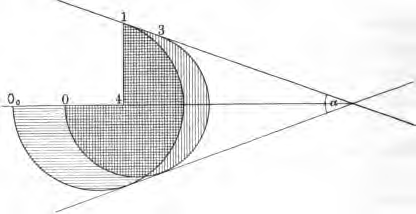
\includegraphics[width=.70\linewidth,height=40mm,keepaspectratio]{fig_assets/fig20_p0182_src_clean_x8.png}
\end{center}

% src-pdfpage=0183
% src-break=0183
vertical schraffirte 13041 von gleicher Fläche, so dass der Bogen $10_0$ sicher kein Extremum der Fläche bei vorgeschriebener Bogenlänge liefert. Der Bogen $\mathfrak{C}_1$ ist die gerade Strecke 13.

\begin{center}
{\large \S~41.}
\end{center}

Der Punkt 0 sei auf der Extremale $\mathfrak{C}$ so gewählt, dass $\xi_t$ nicht verschwindet; dann kann die Differentialgleichung der Extremalen in der Form
\[
f_y+\lambda g_y-\frac{d(f_p+\lambda g_p)}{dx}=0
\]
geschrieben werden, und ergiebt für $\dfrac{dp}{dx}$ einen in Bezug auf $x,y,p$ regulären Ausdruck, wenn die Ungleichung
\begin{equation}\tag{45}
f_{pp}+\lambda g_{pp}\gtrless 0
\end{equation}
besteht. Unter dieser Voraussetzung lehrt dann der allgemeine Satz des \S~27, dass die Differentialgleichung ein Integral von der Form
\begin{equation}\tag{46}
y=\Phi(x,a,b,\lambda)
\end{equation}
besitzt, welches für $a=a_0$, $b=b_0$, $\lambda=\lambda_0$ auf die Curve $\mathfrak{C}$ führt, und in der Stelle $(x_{00},a_0,b_0,\lambda_0)$ regulär ist, wenn durch $x_{00}$ die Abscisse des Punktes 0 bezeichnet wird. Nimmt man speciell für $a$ und $b$ die Werthe von $y$ und $p$ für $x=x_{00}$, so ist
\[
\Phi(x,a,b,\lambda)=a+b(x-x_{00})+[x-x_{00}]_2
\]
und für $x=x_{00}$ ist
\begin{equation}\tag{47}
\Phi_b=0,
\quad \Phi_{bx}=1.
\end{equation}
Wir suchen nun aus der durch die Gleichung (46) gegebenen dreifachen Mannigfaltigkeit von Extremalen eine zweifache auszusondern, welche eine vom Punkte 0 ausgehende reguläre Curve $\mathfrak{C}_0$, deren Gleichung
\[
y_0=\gamma(x_0)
\]
ist, transversal schneiden. Das geschieht, wenn die folgenden Gleichungen erfüllt sind:
\begin{equation}\tag{48}
\begin{aligned}
M&=\Phi(x_0,a,b,\lambda)-\gamma(x_0)=0,\\
N&=f+\lambda g-p(f_p+\lambda g_p)+(f_p+\lambda g_p)\gamma'(x)\big|_{x=x_0}=0;
\end{aligned}
\end{equation}
% src-pdfpage=0184
% src-break=0184
dabei sind in der zweiten Gleichung für $y$ und $p$ die Werthe $\Phi$ und $\Phi_x$ einzusetzen. Die linken Seiten dieser Gleichungen sind an der Stelle $x_0=x_{00}$, $a=a_0$, $b=b_0$, $\lambda=\lambda_0$ regulär; es ist leicht einzusehen, wann man aus ihnen zwei der Grössen $x,a,b,\lambda$ als Functionen der übrigen ausdrücken kann. Bildet man nämlich
\[
\frac{\partial(M,N)}{\partial(x_0,b)}=
\left|\begin{array}{cc}
\Phi_x-\gamma'(x)&\Phi_b\\[.6ex]
\dfrac{\partial N}{\partial x}+\Phi_x\dfrac{\partial N}{\partial y}+\Phi_{xx}\dfrac{\partial N}{\partial p}&
\dfrac{\partial N}{\partial y}\Phi_b+\dfrac{\partial N}{\partial p}\Phi_{bx}
\end{array}\right|_{x=x_0}
\]
und beachtet, dass offenbar
\[
\frac{\partial N}{\partial p}=[\gamma'(x)-\Phi_x](f_{pp}+\lambda g_{pp})\big|_{x=x_0},
\]
so erhält man nach den Gleichungen (47) für $x=x_{00}$
\[
\frac{\partial(M,N)}{\partial(x_0,b)}=-[\gamma'(x)-\Phi_x]^2(f_{pp}+\lambda g_{pp})\big|_{x=x_{00}}
\]
und dieser Ausdruck ist von Null verschieden an der Stelle $(x_{00},a_0,b_0,\lambda_0)$, wenn
\[
\Phi_x(x_{00},a_0,b_0,\lambda_0)-\gamma'(x_{00})\gtrless 0,
\]
d.~h. wenn die Curven $\mathfrak{C}$ und $\mathfrak{C}_0$ einander nicht berühren. Alsdann ergeben die Gleichungen (48) für $b-b_0$ und $x_0-x_{00}$ Ausdrücke von der Form
\[
[a-a_0,\lambda-\lambda_0]_1;
\]
setzt man ersteren in $\Phi$ für $b-b_0$ ein, so erhält man einen Ausdruck
\begin{equation}\tag{49}
y=\varphi(x,a,\lambda),
\end{equation}
der in der Stelle $(x_{00},a_0,\lambda_0)$ regulär ist und die zweifach unendlich vielen, die Curve $\mathfrak{C}_0$ transversal schneidenden Extremalen definirt. Zieht sich die Curve $\mathfrak{C}_0$ in den Punkt 0 zusammen, so ergiebt sich dasselbe Resultat, d.~h. eine Gleichung der durch diesen gehenden Extremalen einfach, indem man die Gleichung
\begin{equation}\tag{50}
\Phi(x_{00},a,b,\lambda)-y_{00}=0
\end{equation}
nach $b$ auflöst.

In jedem dieser Fälle ist zwischen $a,b,\lambda$ ein Zusammenhang durch eine Gleichung
\begin{equation}\tag{51}
\Omega(a,b,\lambda)=0
\end{equation}
hergestellt, für welche
% src-pdfpage=0185
% src-break=0185
\begin{equation}\tag{52}
\Omega_b(a_0,b_0,\lambda_0)\gtrless 0
\end{equation}
und die linke Seite in der Umgebung der Stelle $(a_0,b_0,\lambda_0)$ regulär ist. Dabei erhält man offenbar
\[
\Omega_a+\Omega_b\frac{\partial b}{\partial a}=0,
\quad
\Omega_\lambda+\Omega_b\frac{\partial b}{\partial \lambda}=0,
\]
\[
\varphi_a(x,a,\lambda)=\Phi_a+\Phi_b\frac{\partial b}{\partial a},
\quad
\varphi_\lambda(x,a,\lambda)=\Phi_\lambda+\Phi_b\frac{\partial b}{\partial\lambda},
\]
und analoge Gleichungen gelten für jede Grösse, welche zuerst als Function von $a,b,\lambda$ erscheint, und dann in eine solche von $a$ und $\lambda$ allein übergeht.

Setzt man z.~B.
\[
\Theta(x,a,b,\lambda)=\int_{x_0}^{x}g(x,\Phi,\Phi_x)\,dx
\]
und geht diese Grösse bei der Annahme (51) in $\omega(x,a,\lambda)$ über, so hat sie für die Extremalen (49), da $t=x$ gesetzt werden kann, dieselbe Bedeutung wie früher die Grösse $\omega(t,a,b)$, und man erhält für $\Delta$, indem man $b$ durch $\lambda$ ersetzt, folgenden Ausdruck:
\[
\begin{aligned}
\Delta&=\frac{\partial(\xi,\eta,\omega)}{\partial(x,a,\lambda)}
=\frac{\partial(\varphi,\omega)}{\partial(a,\lambda)} \\
&=\begin{vmatrix}
\Phi_a+\Phi_b\dfrac{\partial b}{\partial a}&\Phi_\lambda+\Phi_b\dfrac{\partial b}{\partial\lambda}\\[1.0ex]
\Theta_a+\Theta_b\dfrac{\partial b}{\partial a}&\Theta_\lambda+\Theta_b\dfrac{\partial b}{\partial\lambda}
\end{vmatrix}\\
&=\frac{1}{\Omega_b}\begin{vmatrix}
\Phi_a&\Phi_b&\Phi_\lambda\\
\Omega_a&\Omega_b&\Omega_\lambda\\
\Theta_a&\Theta_b&\Theta_\lambda
\end{vmatrix}=\frac{D}{\Omega_b}.
\end{aligned}
\]
Gelingt es zu beweisen, dass diese Determinante nicht identisch verschwindet, so ist gezeigt, dass die Extremalen $y=\varphi(x,a,\lambda)$ wenigstens in der Umgebung des Punktes 0 ein Feld im Sinne des \S~39 bilden.

Um die zuletzt erhaltene Determinante zu untersuchen, gehen wir davon aus, dass $x_0$ als reguläre Function von $a,b,\lambda$ definirt ist; man hat daher die Gleichung
\[
\Theta_a=-g\frac{\partial x_0}{\partial a}\bigg|^0+\int_{x_0}^{x}\frac{\partial g}{\partial a}\,dx
=-g\frac{\partial x_0}{\partial a}\bigg|^0+g_p\Phi_a\bigg|_{x_0}^{x}+\int_{x_0}^{x}\left(g_y-\frac{dg_p}{dx}\right)\Phi_a\,dx
\]
% src-pdfpage=0186
% src-break=0186
nebst ähnlichen, in welchen $a$ durch $b$ oder $\lambda$ ersetzt ist. Hieraus folgt
\[
D=\frac{\partial(\Phi,\Omega,\Theta)}{\partial(a,b,\lambda)}
\]
\[
=\begin{vmatrix}
\Phi_a&\Phi_b&\Phi_\lambda\\[.6ex]
\Omega_a&\Omega_b&\Omega_\lambda\\[.6ex]
A+\displaystyle\int_{x_0}^{x}\left(g_y-\frac{dg_p}{dx}\right)\Phi_a\,dx&B+\displaystyle\int_{x_0}^{x}\left(g_y-\frac{dg_p}{dx}\right)\Phi_b\,dx&C+\displaystyle\int_{x_0}^{x}\left(g_y-\frac{dg_p}{dx}\right)\Phi_\lambda\,dx
\end{vmatrix},
\]
wobei die Grössen $A,B,C$ von $x$ unabhängig sind; denn die in den Ausdrücken $\Theta_a,\Theta_b,\Theta_\lambda$ vor dem Integralzeichen stehenden Glieder, welche von $x$ abhängen, fallen weg, wenn man die erste Reihe der Determinante mit $g_p$ multiplicirt und von der letzten subtrahirt. Wenn nun dieser Ausdruck $D$ identisch verschwände, so könnten erstens zugleich die Determinanten zweiter Ordnung der Matrix
\begin{equation}\tag{53}
\left\|\begin{array}{ccc}
\Omega_a&\Omega_b&\Omega_\lambda\\[.8ex]
A+\displaystyle\int_{x_0}^{x}\cdots&B+\displaystyle\int_{x_0}^{x}\cdots&C+\displaystyle\int_{x_0}^{x}\cdots
\end{array}\right\|
\end{equation}
identisch verschwinden. Die Differentialquotienten derselben nach $x$ sind die Determinanten der Matrix
\[
\left\|\begin{array}{ccc}
\Omega_a&\Omega_b&\Omega_\lambda\\[.8ex]
\left(g_y-\dfrac{dg_p}{dx}\right)\Phi_a&
\left(g_y-\dfrac{dg_p}{dx}\right)\Phi_b&
\left(g_y-\dfrac{dg_p}{dx}\right)\Phi_\lambda
\end{array}\right\|;
\]
da nun auf der Curve $\mathfrak{C}$ als Extremale im Problem des relativen Extremums die Grösse
\[
R=g_y-\frac{dg_p}{dx}
\]
nicht verschwindet, so würden auch die Determinanten der Matrix
\[
\left\|\begin{array}{ccc}
\Omega_a&\Omega_b&\Omega_\lambda\\
\Phi_a&\Phi_b&\Phi_\lambda
\end{array}\right\|
\]
verschwinden, z.~B.
\begin{equation}\tag{54}
\Omega_a\Phi_b-\Omega_b\Phi_a=0,
\quad
\Omega_\lambda\Phi_b-\Omega_b\Phi_\lambda=0.
\end{equation}
Die erste dieser Gleichungen ist aber offenbar unmöglich, da für $x=x_{00}$, $a=a_0$, $b=b_0$, $\lambda=\lambda_0$
% src-pdfpage=0187
% src-break=0187
\begin{equation}\tag{55}
\Phi_a=1,
\quad \Phi_b=0,
\quad \Omega_b\gtrless 0;
\end{equation}
die zweite deshalb, weil $\Phi_b$ mit der ersten, $\Phi_\lambda$ mit einer höheren Potenz von $x-x_{00}$ beginnt; die Grösse $\Phi_\lambda$ kann nicht identisch verschwinden, weil sonst der Ausdruck $\Phi$ von $\lambda$ unabhängig wäre, mithin auch der Gleichung
\[
f_y-\frac{df_p}{dx}=0
\]
genügen würde, deren linke Seite ebenso wie $R$ für die Curve $\mathfrak{C}$ von Null verschieden ist.

Speciell folgt aus dieser Betrachtung, dass keine der Determinanten
\begin{equation}\tag{56}
\left|\begin{array}{cc}
\Omega_a&\Omega_b\\[.8ex]
A+\displaystyle\int_{x_0}^{x}R\Phi_a\,dx&B+\displaystyle\int_{x_0}^{x}R\Phi_b\,dx
\end{array}\right|,
\quad
\left|\begin{array}{cc}
\Omega_\lambda&\Omega_b\\[.8ex]
C+\displaystyle\int_{x_0}^{x}R\Phi_\lambda\,dx&B+\displaystyle\int_{x_0}^{x}R\Phi_b\,dx
\end{array}\right|
\end{equation}
identisch verschwindet, da ihre Ableitungen die linken Seiten der Gleichungen (54) sind, multiplicirt mit der von Null verschiedenen Grösse $R$. Nach einem allgemeinen Satze der Determinantentheorie sind aber in einer verschwindenden Determinante die Adjuncten zweier Parallelreihen proportional; wendet man diesen Satz auf die erste und dritte Zeile der Determinante $D$ an, so ergiebt sich, dass die letzten beiden Determinanten den linken Seiten der Gleichungen (54) proportional sind. Da nun weder eine dieser vier Grössen identisch verschwindet, noch die Grösse $R$, so ergiebt sich, dass die logarithmischen Ableitungen der Grössen (56) nach $x$ gleich sind, die Grössen selbst also in der Beziehung
\[
\left|\begin{array}{cc}
\Omega_a&\Omega_b\\[.8ex]
A+\displaystyle\int_{x_0}^{x}R\Phi_a\,dx&B+\displaystyle\int_{x_0}^{x}R\Phi_b\,dx
\end{array}\right|
=M
\left|\begin{array}{cc}
\Omega_\lambda&\Omega_b\\[.8ex]
C+\displaystyle\int_{x_0}^{x}R\Phi_\lambda\,dx&B+\displaystyle\int_{x_0}^{x}R\Phi_b\,dx
\end{array}\right|
\]
% src-pdfpage=0188
% src-break=0188
stehen, wenn durch $M$ eine von $x$ unabhängige, endliche und von Null verschiedene Grösse bezeichnet wird. Hieraus folgt durch Differentiation mit Rücksicht auf den nicht verschwindenden Werth der Grösse $R$
\[
\Omega_a\Phi_b-\Omega_b\Phi_a=M(\Omega_\lambda\Phi_b-\Omega_b\Phi_\lambda).
\]
Setzen wir hier $x=x_{00}$, so reducirt sich die linke Seite auf $-\Omega_b$, die rechte auf Null, da die Relationen (55) gelten. Die Annahme, $D$ verschwinde identisch, führt also stets auf einen Widerspruch.

Auf Grund der Beziehung zwischen $D$ und $\Delta$ ist hiermit Folgendes bewiesen. Fügen wir zu den früheren Voraussetzungen betreffs der Extremale $\mathfrak{C}$ die Ungleichung (45) hinzu, so kann der im Punkte 0 beginnende Bogen stets mit einem Felde umgeben werden, dessen Extremalen entweder alle durch den Punkt 0 gehen, oder eine gegebene, von der Curve $\mathfrak{C}$ im Punkte 0 transversal geschnittene, nicht berührte reguläre Curve $\mathfrak{C}_0$ transversal schneiden. Für einen hinreichend kleinen Extremalenbogen ist also die \textsc{Jacobi}'sche Bedingung des Extremums erfüllt, gleichviel ob ein oder beide Endpunkte der gesuchten Curve festgehalten werden.

\begin{center}
{\large \S~42.}
\end{center}

Ist der Punkt 0 fest und wird die Gleichung $\Omega=0$ demgemäss durch die specielle Relation (50) ersetzt, so hat man
\[
\Omega_a=\Phi_a(x_0,a,b,\lambda),
\]
\[
\Omega_b=\Phi_b(x_0,a,b,\lambda),
\quad
\Omega_\lambda=\Phi_\lambda(x_0,a,b,\lambda)
\]
und erhält daher
\[
D=\frac{\partial\left\{\Phi(x,a,b,\lambda),\ \Phi(x_0,a,b,\lambda),\ \displaystyle\int_{x_0}^{x}g[x,\Phi(x,a,b,\lambda),\Phi_x(x,a,b,\lambda)]\,dx\right\}}{\partial(a,b,\lambda)}.
\]
Da nun dieser Ausdruck den Werth
\[
\Delta\Phi_b(x_0,a,b,\lambda)
\]
hat, so verschwindet die Grösse
\[
\Delta(x_0,x)=D\big|_{a=a_0,\,b=b_0,\,\lambda=\lambda_0}
\]
% src-pdfpage=0189
% src-break=0189
wenn die Punkte 0 und $(x,y)$ conjugirt sind. Damit ist das von \textsc{Mayer} aufgestellte Kennzeichen der conjugirten Punkte abgeleitet. Die analoge Formel von \textsc{Weierstrass} erhält man unter der Annahme, dass die Extremalen in der Form
\begin{equation}\tag{57}
x=X(t,a,b,\lambda),
\quad y=Y(t,a,b,\lambda)
\end{equation}
dargestellt sind; dann hat man die Identität
\[
Y=\Phi(X,a,b,\lambda)
\]
und die aus ihr folgenden Relationen
\[
\begin{gathered}
Y_t=\Phi_x(X,a,b,\lambda)X_t,
\quad Y_a=\Phi_xX_a+\Phi_a,
\quad Y_b=\Phi_xX_b+\Phi_b,\\
Y_\lambda=\Phi_xX_\lambda+\Phi_\lambda;
\end{gathered}
\]
\[
X_t\Phi_a=X_tY_a-X_aY_t=\theta_1(t),
\]
\[
X_t\Phi_b=X_tY_b-X_bY_t=\theta_2(t),
\quad
X_t\Phi_\lambda=X_tY_\lambda-X_\lambda Y_t=\theta_3(t).
\]
Gehört daher der Punkt 0 zum Argument $t=t_0$, so ergiebt sich
\[
D X_t(t,a,b,\lambda)X_t(t_0,a,b,\lambda)=
\begin{vmatrix}
\theta_1(t)&\theta_2(t)&\theta_3(t)\\
\theta_1(t_0)&\theta_2(t_0)&\theta_3(t_0)\\[.6ex]
\dfrac{\partial K}{\partial a}&\dfrac{\partial K}{\partial b}&\dfrac{\partial K}{\partial\lambda}
\end{vmatrix},
\]
wobei gesetzt ist
\[
K=\int_{x_0}^{x}g\,dx=\int_{t_0}^{t}G(X,Y,X_t,Y_t)\,dt.
\]
Nun hat man, da $x_0$ von $a,b,\lambda$ nicht abhängt, die Gleichung
\[
\frac{\partial K}{\partial a}=\Phi_a g_p\bigg|_{x_0}^{x}+\int_{x_0}^{x}\Phi_a\left(g_y-\frac{dg_p}{dx}\right)dx
\]
nebst ähnlichen Formeln, in welchen $a$ durch $b$ und $\lambda$ ersetzt ist; addirt man also in der Determinante $D$ die ersten Reihen mit passenden Factoren multiplicirt zur letzten, so wird diese:
\[
\int_{x_0}^{x}\Phi_a\left(g_y-\frac{dg_p}{dx}\right)dx,
\quad
\int_{x_0}^{x}\Phi_b\left(g_y-\frac{dg_p}{dx}\right)dx,
\quad
\int_{x_0}^{x}\Phi_\lambda\left(g_y-\frac{dg_p}{dx}\right)dx.
\]
Weiter hat man nach \S~5, wenn
\[
G(x,y,x',y')=x'g\left(x,y,\frac{y'}{x'}\right)
\]
eingeführt wird,
% src-pdfpage=0190
% src-break=0190
\[
x'\left(g_y-\frac{dg_p}{dx}\right)=G_y-G'_{y'}=-\frac{x'}{y'}(G_x-G'_{x'});
\]
hieraus folgt
\[
\Phi_a\left(g_y-\frac{dg_p}{dx}\right)dx=\biggl(Y_a-X_a\frac{Y_t}{X_t}\biggr)(G_y-G'_{y'})dt
\]
\[
=[X_a(G_x-G'_{x'})+Y_a(G_y-G'_{y'})]dt.
\]
Setzt man daher
\[
\Theta_1(t_0,t)=\int_{t_0}^{t}dt\,[X_a(G_x-G'_{x'})+Y_a(G_y-G'_{y'})]
\]
und lässt hieraus $\Theta_2$ und $\Theta_3$ entstehen, indem man $a$ durch $b$ und $\lambda$ ersetzt, so erhält man die \textsc{Weierstrass}'sche Determinante
\[
D X_t(t,a,b,\lambda)X_t(t_0,a,b,\lambda)=
\begin{vmatrix}
\theta_1(t)&\theta_2(t)&\theta_3(t)\\
\theta_1(t_0)&\theta_2(t_0)&\theta_3(t_0)\\
\Theta_1(t_0,t)&\Theta_2(t_0,t)&\Theta_3(t_0,t)
\end{vmatrix}=D(t_0,t).
\]
Dabei ist zu beachten, dass $D$ nur definirt ist unter der Voraussetzung, dass in dem Intervall $t_0\ldots t$ überall $y$ als reguläre Function von $x$ durch die Curve $\mathfrak{C}$ definirt sei. Die rechte Seite dagegen hat für jeden Bogen $\mathfrak{C}$ Sinn, längs dessen $x$ und $y$ reguläre Functionen von $t$ sind und die Grösse $H_1(x,y,x',y')$ nicht verschwindet; denn ein solcher kann nach \S~27 stets in eine Curvenschar, wie sie durch die Gleichungen (57) dargestellt wird, eingebettet werden.

Wenn $D(t_0,t)$ nicht identisch verschwindet, so ist mindestens eine der Grössen $\theta_1(t_0),\theta_2(t_0),\theta_3(t_0)$ von Null verschieden. Es sei dies z.~B. die letzte; dann können $t_0$ und $\lambda$ aus den Gleichungen
\[
x_0=X(t_0,a,b,\lambda),
\quad y_0=Y(t_0,a,b,\lambda)
\]
als reguläre Functionen von $a$ und $b$ ausgerechnet werden; substituirt man dieselben, so erhält man
\[
X=\xi(t,a,b),
\quad Y=\eta(t,a,b).
\]
Dann gelten folgende Gleichungen:
\[
X_t\frac{\partial t_0}{\partial a}+X_\lambda\frac{\partial\lambda}{\partial a}+X_a\bigg|^{t_0}=Y_t\frac{\partial t_0}{\partial a}+Y_\lambda\frac{\partial\lambda}{\partial a}+Y_a\bigg|^{t_0}=0,
\]
\[
X_t\frac{\partial t_0}{\partial b}+X_\lambda\frac{\partial\lambda}{\partial b}+X_b\bigg|^{t_0}=Y_t\frac{\partial t_0}{\partial b}+Y_\lambda\frac{\partial\lambda}{\partial b}+Y_b\bigg|^{t_0}=0,
\]
% src-pdfpage=0191
% src-break=0191
\[
\xi_t=X_t,
\quad \eta_t=Y_t,
\quad X_a+X_\lambda\frac{\partial\lambda}{\partial a}=\xi_a,
\quad Y_a+Y_\lambda\frac{\partial\lambda}{\partial a}=\eta_a,
\]
\[
X_b+X_\lambda\frac{\partial\lambda}{\partial b}=\xi_b,
\quad Y_b+Y_\lambda\frac{\partial\lambda}{\partial b}=\eta_b.
\]
Aus den ersten vier Gleichungen folgt leicht
\[
\theta_1(t_0)+\theta_3(t_0)\frac{\partial\lambda}{\partial a}=\theta_2(t_0)+\theta_3(t_0)\frac{\partial\lambda}{\partial b}=0,
\]
aus den letzten vier
\[
\theta_1(t)+\theta_3(t)\frac{\partial\lambda}{\partial a}=\xi_t\eta_a-\xi_a\eta_t,
\quad
\theta_2(t)+\theta_3(t)\frac{\partial\lambda}{\partial b}=\xi_t\eta_b-\xi_b\eta_t,
\]
und die Definition der Grössen $\Theta$ ergiebt
\[
\Theta_1(t_0,t)+\frac{\partial\lambda}{\partial a}\Theta_3(t_0,t)=
\int_{t_0}^{t}dt\{(G_x-G'_{x'})\xi_a+(G_y-G'_{y'})\eta_a\}=A,
\]
\[
\Theta_2(t_0,t)+\frac{\partial\lambda}{\partial b}\Theta_3(t_0,t)=
\int_{t_0}^{t}dt\{(G_x-G'_{x'})\xi_b+(G_y-G'_{y'})\eta_b\}=B.
\]
Addirt man daher in der Determinante $D(t_0,t)$ die dritte Verticalreihe mit $\partial\lambda:\partial a$ und $\partial\lambda:\partial b$ multiplicirt zur ersten und zweiten, so erhält man
\[
D(t_0,t)=-\theta_3(t_0)\begin{vmatrix}
\xi_t\eta_a-\xi_a\eta_t&\xi_t\eta_b-\xi_b\eta_t\\
A&B
\end{vmatrix}.
\]
Da nun nach \S~35
\[
\omega_a=G_{x'}\xi_a+G_{y'}\eta_a+A,
\quad
\omega_b=G_{x'}\xi_b+G_{y'}\eta_b+B,
\]
\[
\omega_t=G=\xi_tG_{x'}+\eta_tG_{y'},
\]
so folgt endlich
\[
D(t_0,t)=-\theta_3(t_0)\frac{\partial(\xi,\eta,\omega)}{\partial(t,a,b)}=-\theta_3(t_0)\Delta.
\]
Unter der eingeführten Voraussetzung verschwinden also $\Delta$ und $D(t_0,t)$ nur gleichzeitig, und die Gleichung
\[
D(t_0,t)=0
\]
ist, sobald ihre linke Seite nicht identisch verschwindet, eine hinreichende und nothwendige Bedingung dafür, dass zu den Argumenten $t_0$ und $t$ conjugirte Punkte gehören. Ist daher die Grösse $D(t_0,t)$, abgesehen vom Punkte 0 selbst, auf einem Bogen 02 überall von Null verschieden, so ergiebt sich ein Extremum
% src-pdfpage=0192
% src-break=0192
 der gesuchten Art für jeden Bogen 12, dessen Anfangspunkt von 0 beliebig wenig verschieden ist.

Hieraus folgt auf Grund der am Schluss des \S~31 durchgeführten Betrachtung, dass für den Bogen 12 bei festen Endpunkten die \textsc{Jacobi}'sche Bedingung des Extremums im Allgemeinen auch folgendermaassen formulirt werden kann: die Gleichung
\[
D(t_1,t)=0
\]
besitzt auf der Strecke 12 keine Wurzel ausser $t=t_1$; jene Betrachtung lässt sich nämlich ohne jede Abänderung auf die jetzt durch $D(t_0,t)$ bezeichnete Grösse anwenden, sobald die Ungleichung
\[
\frac{\partial D(t_0,t)}{\partial t}\bigg|_{t=t_0}\gtrless 0
\]
besteht. Auch wenn die Grössen
\[
d_\alpha(t_0)=\frac{\partial^\alpha D(t_0,t)}{\partial t^\alpha}\bigg|_{t=t_0}
\]
für $\alpha=1,2,\ldots n$ identisch verschwinden, $d_{n+1}(t_1)$ aber von Null verschieden ist, braucht die Argumentation des \S~31 nur insofern modificirt zu werden, als die Grösse $d_{n+1}(t_0)$ an Stelle von $f_1(t_0)$ tritt. Nur wenn $d_{n+1}(t_0)$ nicht identisch verschwindet, $d_{n+1}(t_1)$ aber den Werth Null hat, wird es zweifelhaft, ob die citirte Betrachtung anzuwenden ist.


% machine-manifest-begin
% {"work": "Kneser_LVR", "language": "de", "branch": "canonical_complete_volume", "source_pdf_pages": "author-clean cumulative p0011-p0335; sections 1-69, Literature, printed errata, and unnumbered addendum complete; p0336 rear board excluded by evidence ledger", "visible_text_policy": "authorial text only; no vendor marks, source captions, running heads, page numbers, signatures, or preservation/library notes", "math_policy": "all displayed and inline mathematical symbols retained as TeX; provenance appears only in comments and external ledgers", "figure_policy": "figures 1--24 retained as HQ source-derived whitened original crops only; no visible drawn/TikZ layer", "description": "complete diplomatic German edition", "completion_boundary": "source PDF335; PDF336 rear board excluded", "errata_policy": "printed errata transcribed as printed; body corrections not silently applied"}
% machine-manifest-end

% machine-unit: Kneser_LVR_DE_p0193_p0206 §§43-45
% src-pdfpage=0193
\begin{center}
{\large Fünfter Abschnitt.}\\[1.1ex]
{\Large\bfseries Discontinuirliche Lösungen.}\\[2ex]
\rule{32mm}{0.4pt}\\[2ex]
{\large \S~43.}
\end{center}

Die Entwickelungen der vorhergehenden Abschnitte geben nicht immer eine Lösung der ursprünglichen Extremumsaufgabe, zwischen zwei gegebenen Punkten eine Curve zu ziehen, welche ein absolutes oder relatives Extremum des Integrals $J$ liefert. Es wurde nur gezeigt, dass die gesuchte Curve, wenn sie gewisse Stetigkeitseigenschaften haben soll, nichts anderes sein kann, als ein reguläres Stück einer Extremale; sodann wurden Bedingungen des Extremums abgeleitet unter der Voraussetzung, dass die beiden gegebenen Endpunkte der gesuchten Curve schon durch einen von Singularitäten freien Bogen einer Extremale verbunden seien. Ist diese Voraussetzung nicht erfüllt, was schon bei einfachen Aufgaben vorkommt, so kann das gesuchte Extremum von einer Curve mit den vorausgesetzten Stetigkeitseigenschaften nicht geliefert werden, und so kommt man zu der Frage, ob nicht eine mit Singularitäten, z.~B. Ecken behaftete Curve die vorgelegte Aufgabe löst. Gelingt es, diese Frage zu beantworten, indem man bestimmte Gattungen von Singularitäten zulässt, so hat man zwar auch noch keine unfehlbare Methode zur Bestimmung des gesuchten Extremums, aber der Kreis der Fälle, in denen die Aufgabe gelöst werden kann, erweitert sich.

Speciell fragen wir, wann das Integral
\[
J=\int Fdt
\]
zu einem absoluten Extremum gemacht wird durch eine Curve, welche aus einer endlichen Anzahl in Ecken zusammenstossender
% src-pdfpage=0194
Stücke besteht, deren jedes die früher für die ganze Curve geforderten Eigenschaften besitzt; d.~h. längs jedes Stückes seien $x$ und $y$ stetige, mit stetigen ersten und zweiten Ableitungen versehene Functionen eines Parameters $t$. Für jedes einzelne dieser Stücke bleiben die Betrachtungen des zweiten Abschnitts gültig, da man die Ecken ungeändert lassen und die Variation auf das Innere der Stücke beschränken kann; jedes von ihnen muss daher ein Bogen einer Extremale sein.

\begin{center}
{\small Fig. 21.}\par\vspace{1mm}
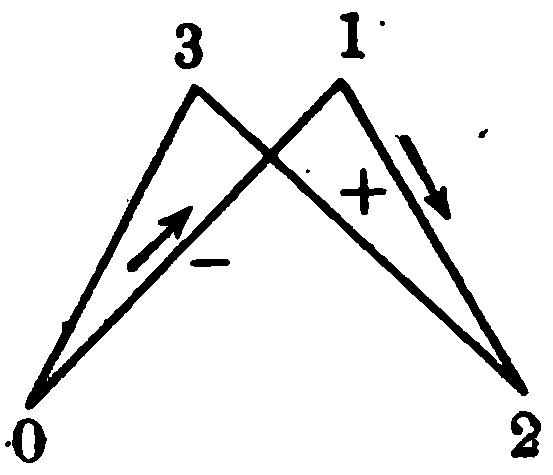
\includegraphics[width=.34\linewidth,height=33mm,keepaspectratio]{fig_assets/fig21_p0194_src_clean_x8.png}
\end{center}

Auf den in der Ecke 1 zusammenstossenden Bögen seien die Punkte 0 und 2 so nahe der Ecke angenommen, dass die Bögen 01 und 12 kein Paar conjugirter Punkte enthalten (Fig.~21). Dann können die Punkte 0 und 2 mit jedem von 1 hinreichend wenig entfernten Punkte 3 durch Extremalen 03 und 32 verbunden werden, und diese können nach \S~2 als Variation der Bögen 01 und 12 betrachtet werden. Die gebrochene Linie 012 als Theil der gesuchten Curve kann daher, indem die Variationsformeln des \S~2 für jeden der Theile 01 und 02 gültig bleiben, durch 032 ersetzt werden. Setzt man nun
\[
\delta x_1=x_3-x_1,\quad \delta y_1=y_3-y_1
\]
und versieht das Symbol irgend einer Grösse mit dem Zeichen $-$, $+$, je nachdem dieselbe für den Bogen 01 in der Richtung über 1 hinaus, oder für den Bogen 12 in der Richtung nach 2 hin gebildet werden soll, so hat man die Formeln
\[
\Delta \overline{J}_{01}=F_{x'}^-\delta x+F_{y'}^-\delta y\big|^1+[\delta x_1,\delta y_1]_2,
\]
\[
\Delta \overline{J}_{12}=-F_{x'}^+\delta x-F_{y'}^+\delta y\big|^1+[\delta x_1,\delta y_1]_2,
\]
\[
F_{x'}^- =F_{x'}(x,y,x'_{-},y'_{-}),\quad
F_{x'}^+=F_{x'}(x,y,x'_{+},y'_{+}),\ldots,
\]
also wenn man addirt,
\[
\Delta\overline{J}_{012}=(F_{x'}^- -F_{x'}^+)\delta x+(F_{y'}^- -F_{y'}^+)\delta y\big|^1+[\delta x_1,\delta y_1]_2.
\]
Diese Grösse muss ein constantes Vorzeichen haben, wenn die Curve, welcher der Linienzug 012 angehört, ein Extremum des Integrals $J$ ergeben soll. Ist daher der Eckpunkt 3 in der Nähe der Lage 1 frei verfügbar, die Grössen $\delta x_1$, $\delta y_1$ also von einander unabhängig, so müssen (\S~7) die Coëfficienten der linearen Glieder verschwinden, und man erhält den Satz von \textsc{Erdmann}
% src-pdfpage=0195
\begin{equation}\tag{1}
F_{x'}^- =F_{x'}^+,
\quad F_{y'}^- =F_{y'}^+.
\end{equation}
Wenn dagegen der Eckpunkt von vornherein an die Curve
\begin{equation}\tag{2}
h(x_1,y_1)=0
\end{equation}
gebunden ist, so dass die Gleichung
\[
0=h_x(x_1,y_1)\delta x_1+h_y(x_1,y_1)\delta y_1+[\delta x_1,\delta y_1]_2
\]
besteht, so kann $\Delta\overline{J}_{012}$ nach \S~7 nur dann ein unabänderliches Vorzeichen haben, wenn
\[
\begin{vmatrix}
F_{x'}^- -F_{x'}^+&F_{y'}^- -F_{y'}^+\\
h_x(x_1,y_1)&h_y(x_1,y_1)
\end{vmatrix}=0,
\]
d.~h. wenn bei einer unendlich kleinen Verschiebung des Punktes 1 auf der Curve (2) die Gleichung
\begin{equation}\tag{3}
F_{x'}^-\delta x_1+F_{y'}^-\delta y_1=F_{x'}^+\delta x_1+F_{y'}^+\delta y_1
\end{equation}
gilt.

Bezeichnet man die Strecke 13 durch $\delta s$, und nimmt an, dass $t$ auf jeder der Extremalen 01 und 12 den Bogen bedeute, der immer in der Richtung von 0 über 1 nach 2 hin wachse, so kann man drei Winkel $\sigma$, $\theta_+$, $\theta_-$ einführen, welche folgenden Gleichungen genügen
\[
\delta x_1=\delta s\cos\sigma,\quad \delta y_1=\delta s\sin\sigma,
\]
\[
x'_{-}=\cos\theta_{-},\quad y'_{-}=\sin\theta_{-},\quad
x'_{+}=\cos\theta_{+},\quad y'_{+}=\sin\theta_{+}.
\]
Man definire ferner die Grössen $u$, $v$ durch die Gleichungen
\begin{equation}\tag{4}
\delta x_1=x'_{+}u+x'_{-}v,
\quad \delta y_1=y'_{+}u+y'_{-}v;
\end{equation}
dann ergiebt sich leicht
\[
u=\frac{\delta s\sin(\sigma-\theta_{-})}{\sin(\theta_{+}-\theta_{-})},
\quad
v=\frac{\delta s\sin(\sigma-\theta_{+})}{\sin(\theta_{-}-\theta_{+})}
\]
und diese Grössen sind den Lothen proportional, welche vom Punkte 3 auf die Extremalen 01 und 12 gefällt werden können. Dabei ergeben die Gleichungen (4)
\[
(F_{x'}^- -F_{x'}^+)\delta x_1+(F_{y'}^- -F_{y'}^+)\delta y_1
\]
\[
=u(x'_{+}F_{x'}^-+y'_{+}F_{y'}^- -F^+)-v(x'_{-}F_{x'}^+ + y'_{-}F_{y'}^+ -F^-)
\]
\[
=u\mathfrak{E}(x_1,y_1,x'_{-},y'_{-},x'_{+},y'_{+})
-v\mathfrak{E}(x_1,y_1,x'_{+},y'_{+},x'_{-},y'_{-}),
\]
und dieser Ausdruck muss nach dem Obigen bei jeder erlaubten Verschiebung des Eckpunkts verschwinden.
% src-pdfpage=0196

\textbf{Erstes Beispiel.} Das Princip der kleinsten Action in der \textsc{Euler-Jacobi}'schen Form bei der Centralbewegung eines freien Punktes in der Ebene. Die Abstossung sei z.~B. der Entfernung proportional; setzt man
\[
r=\sqrt{x^2+y^2},
\]
so ist das Potential $cr$ und das bezeichnete Princip sagt aus, dass die Bahncurven das Integral
\[
\int \sqrt{cr+h}\,\sqrt{dx^2+dy^2}
\]
zum Minimum machen, wobei $h$ die Constante der lebendigen Kraft bedeutet. Nimmt man speciell $h=0$ an, so sind unter den hierdurch definirten Bahncurven die vom Kraftcentrum ausgehenden Radien enthalten, längs deren der bewegte Punkt sich dem Centrum asymptotisch annähern kann, und man hat zu setzen
\[
F=\sqrt{x^2+y^2}\,\sqrt{x'^2+y'^2}.
\]
Die Gleichungen (1) ergeben, wenn $r$ von Null verschieden ist, das Resultat
\[
\frac{x'_{-}}{\sqrt{x_{-}'{}^2+y_{-}'{}^2}}
=
\frac{x'_{+}}{\sqrt{x_{+}'{}^2+y_{+}'{}^2}},
\quad
\frac{y'_{-}}{\sqrt{x_{-}'{}^2+y_{-}'{}^2}}
=
\frac{y'_{+}}{\sqrt{x_{+}'{}^2+y_{+}'{}^2}},
\]
d.~h. die Richtungen $+$, $-$ fallen zusammen. Eine Ecke kann also nur im Kraftcentrum ($r=0$) auftreten. Für irgend zwei von ihm ausgehende Radien sind die Gleichungen (1) erfüllt. Da nun die Radien die einzigen Bahncurven sind, welche bei der Voraussetzung $h=0$ durch das Kraftcentrum gehen, so kann eine gebrochene Linie nur dann ein Extremum liefern, wenn sie aus zwei im Centrum zusammenstossenden geraden Stücken besteht.

Aehnliche Betrachtungen kann man anstellen, wenn die Kraft einer beliebigen Potenz der Entfernung proportional ist; man hat dann das Integral
\[
\int (x^2+y^2)^n\sqrt{dx^2+dy^2}
\]
zu einem Minimum zu machen.

\textbf{Zweites Beispiel.} Aufgabe VII (\S~11). Die kürzeste Linie auf der Fläche, deren Bogenelement durch die Formel
\[
ds^2=Edx^2+2Fdxdy+Gdy^2
\]
% src-pdfpage=0197
gegeben wird, kann nirgends eine frei verfügbare Ecke aufweisen, so lange $EG-F^2$ von Null verschieden ist. Denn die Gleichungen (1) würden erfordern
\[
E\left(\frac{dx}{ds}\right)_{-}+F\left(\frac{dy}{ds}\right)_{-}
=E\left(\frac{dx}{ds}\right)_{+}+F\left(\frac{dy}{ds}\right)_{+},
\]
\[
F\left(\frac{dx}{ds}\right)_{-}+G\left(\frac{dy}{ds}\right)_{-}
=F\left(\frac{dx}{ds}\right)_{+}+G\left(\frac{dy}{ds}\right)_{+},
\]
woraus bei der angegebenen Voraussetzung folgen würde
\[
\left(\frac{dx}{ds}\right)_{-}-\left(\frac{dx}{ds}\right)_{+}
=
\left(\frac{dy}{ds}\right)_{-}-\left(\frac{dy}{ds}\right)_{+}=0.
\]
Wohl aber kann eine Ecke auftreten, wenn verlangt wird, die Punkte 0 und 2 durch die kürzeste Linie zu verbinden, welche mit einer gegebenen Curve einen nicht vorgeschriebenen Punkt 1 gemein hat. Bezeichnet $D$ den Zuwachs beim Fortgang längs dieser Curve, $Ds$ das Bogenelement derselben, so muss die Grösse
\[
\left\{E\left(\frac{dx}{ds}\right)_{-}+F\left(\frac{dy}{ds}\right)_{-}\right\}Dx
+
\left\{F\left(\frac{dx}{ds}\right)_{-}+G\left(\frac{dy}{ds}\right)_{-}\right\}Dy
\]
der Gleichung (3) zufolge ihren Werth behalten, wenn man das Suffix $-$ durch $+$ ersetzt. Sind $ds_+$, $ds_-$ die Elemente der geodätischen Curven 01, 12, so ist jene Grösse $Ds\cos(Ds,ds_-)$; man erhält somit als Bedingung des Extremums
\[
\cos(Ds,ds_-)=\cos(Ds,ds_+).
\]
Die durch die Vorzeichen $+$, $-$ bezeichneten Richtungen der geodätischen Linien liegen also symmetrisch zur Richtung der gegebenen Curve, die beiden Bögen 01, 12 also auf derselben Seite dieser Curve und bilden gleiche spitze Winkel mit ihr.

\begin{center}
{\large \S~44.}
\end{center}

In der Argumentation des \S~8 ist es wesentlich, dass der Grösse $\varepsilon$ positive und negative Werthe beigelegt werden, die gesuchte Curve also mit variirten Curven verglichen wird, welche sowohl nach der einen wie nach der anderen Seite hin von ihr abweichen. Dies ist ausgeschlossen, wenn, wie wir jetzt annehmen wollen, die verglichenen Curven auf ein bestimmtes, durch Schranken umgrenztes Gebiet $\mathfrak{G}$ beschränkt werden, und die untersuchte Curve theilweise mit einer Schranke zusammenfällt; dann gilt die citirte Argumentation nicht mehr, und die
% src-pdfpage=0198
gesuchte Curve braucht nicht überall der Differentialgleichung der Extremalen zu genügen. Es muss daher besonders untersucht werden, wann eine Linie, die zum Theil aus Extremalenbögen besteht, zum Theil mit Schranken zusammenfällt, das Integral $J$ zu einem Extremum machen kann. Dass die mit der Schranke nicht zusammenfallenden Theile Bögen von Extremalen sein müssen, folgt offenbar aus der Erwägung, welche in \S~43 zeigte, dass die gesuchte Curve zwischen den Ecken aus Bögen von Extremalen besteht.

\begin{center}
{\small Fig. 22.}\par\vspace{1mm}
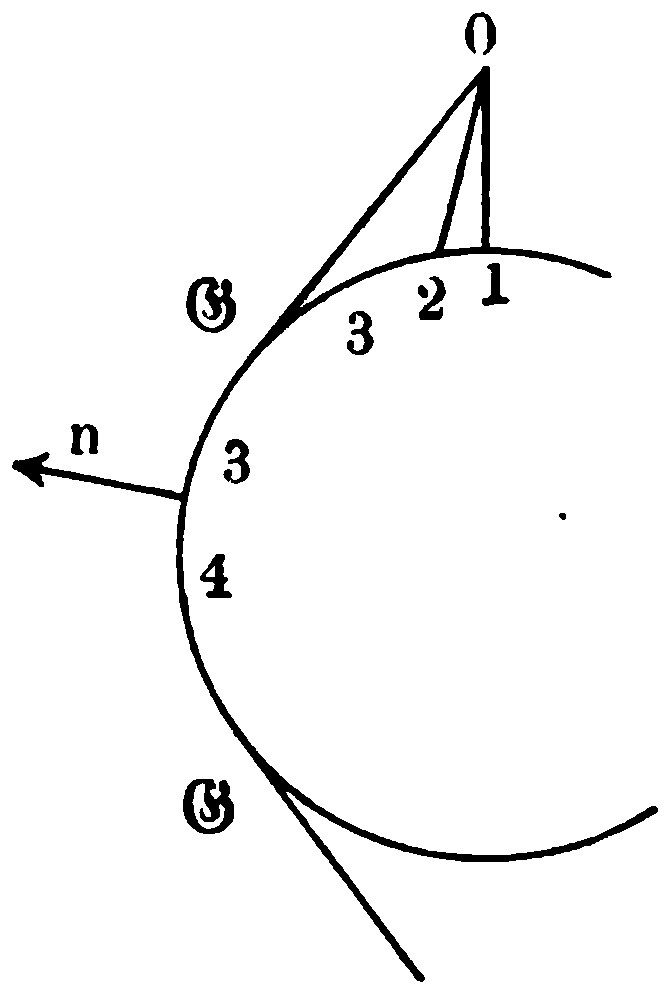
\includegraphics[width=.36\linewidth,height=48mm,keepaspectratio]{fig_assets/fig22_p0198_src_clean_x8.png}
\end{center}

Eine Extremale treffe (Fig.~22) die Schranke im Punkte 1; auf ersterer sei der Punkt 0 so wenig von 1 entfernt, dass der Bogen 01 mit einem Felde umgeben werden kann, dessen Extremalen durch den Punkt 0 gehen. Diesem Felde gehören auch die in der Nachbarschaft des Punktes 1 liegenden Theile der Schranke an, etwa bis zum Punkte 2 hin, und die gebrochene Linie 012 sei ein Theil der combinirten Curve, welche auf das Eintreten des Extremums hin untersucht werden soll. Dann kann für den dem Felde angehörigen Bogen der Schranke alles benutzt werden, was in \S~20 für die Curve $\Omega$ bewiesen wurde; sind $x$ und $y$ längs der Schranke Functionen $\varphi(\tau)$ im Sinne des \S~17, wächst $\tau$ in der Richtung 12, und passirt der Punkt 3 längs der Schranke laufend die Lage 1, so hat man
\[
\frac{d(\overline{J}_{03}+\overline{J}_{32})}{d\tau}
=\mathfrak{E}\left(x,y,x',y',\frac{dx}{d\tau},\frac{dy}{d\tau}\right)\bigg|^3,
\]
wobei sich die Grössen $x'$, $y'$ auf die in der Richtung von 0 nach 1 hin durchlaufene Extremale 01 beziehen. Wenn daher diese Grösse $\mathfrak{E}$ von Null verschieden ist, kann die Summe $\overline{J}_{03}+\overline{J}_{32}$ bei beliebig kleiner Entfernung der Punkte 1 und 3 sowohl grösser wie kleiner werden, als $\overline{J}_{01}+J_{12}$, und letztere Grösse bildet sicher kein Extremum des Integrals $J$. Soll dieses durch den Linienzug 012 geliefert werden, so muss also die Gleichung
\[
\mathfrak{E}\left(x,y,x',y',\frac{dx}{d\tau},\frac{dy}{d\tau}\right)\bigg|^1=0
\]
bestehen, d.~h. entweder müssen Extremale und Schranke sich berühren, und zwar so, dass die Fortgangsrichtung 012 im
% src-pdfpage=0199
Punkte 1 sich stetig ändert, oder die Grösse $\mathfrak{E}$ muss in ausserordentlicher Weise verschwinden.

Eine weitere nothwendige Bedingung des Extremums erhält man, wenn man ein der gesuchten Curve angehöriges Stück 34 der Schranke variirt, und zwar so, dass die Endpunkte festgehalten werden und die Variationen der Coordinaten dieselben Eigenschaften haben wie in \S~2. Setzt man dann
\[
\frac{F_x-F'_{x'}}{y'}=-\frac{F_y-F'_{y'}}{x'}=M,
\]
so ergiebt sich
\[
\delta J=\int M(y'\delta x-x'\delta y)\,dt,
\]
\[
\Delta J=\delta J+\int[\delta x,\delta y,\delta x',\delta y']_2\,dt.
\]
Dabei muss jeder Punkt $(x+\delta x,y+\delta y)$ dem Gebiet $\mathfrak{G}$ angehören, an welches die gesuchte Curve gebunden ist. Bezeichnet man durch $n$ die nach dem Innern von $\mathfrak{G}$ weisende Normale der Schranke, durch $\varepsilon$ eine positive Constante, so werden die ausgesprochenen Forderungen erfüllt durch die Annahme
\[
\delta x=\varepsilon\cos(nx)(t-t_3)^3(t_4-t)^3,
\]
\[
\delta y=\varepsilon\cos(ny)(t-t_3)^3(t_4-t)^3,
\]
und man erhält
\[
\delta J=\varepsilon\int_3^4 [y'\cos(nx)-x'\cos(ny)]M(t-t_3)^3(t_4-t)^3\,dt,
\]
\[
\Delta J=\delta J+[\varepsilon]_2.
\]
Soll daher $\Delta J$ ein festes Vorzeichen besitzen, so muss dasselbe von dem Integral $\delta J:\varepsilon$ gelten, wenn es nicht verschwindet; da nun die Punkte 3 und 4 einander beliebig genähert werden können, so muss die Grösse
\[
[y'\cos(nx)-x'\cos(ny)]M,
\]
wenn sie nicht verschwindet, das von $\Delta J$ verlangte Vorzeichen haben, d.~h. im Falle des Maximums negativ, des Minimums positiv sein. Nun ist die Determinante
\[
\begin{vmatrix}
\cos(nx)&\cos(ny)\\
dx&dy
\end{vmatrix}
\]
positiv oder negativ, je nachdem die Richtung $n$ zu der des Elements $(dx,dy)$, d.~h. zur Integrationsrichtung ebenso oder
% src-pdfpage=0200
entgegengesetzt liegt wie die $+x$-Axe zur $+y$-Axe oder, was dasselbe bedeutet, je nachdem das Gebiet $\mathfrak{G}$ im negativen oder positiven Sinne bei der Integration umlaufen wird. Im ersten Falle folgt also, wenn ein Maximum eintreten soll,
\[
M\leqq 0,
\]
wenn ein Minimum gesucht wird,
\[
M\geqq 0;
\]
im zweiten Falle vertauschen diese Ungleichungen ihre Bedeutung.

\textbf{Erstes Beispiel.} Zwischen zwei Punkten der Ebene die kürzeste Linie zu ziehen, welche die Schranken eines gegebenen Gebietes $\mathfrak{G}$ nicht überschreitet.

Die Aufgabe bietet nur dann Interesse, wenn die gerade Verbindung der beiden Punkte die Schranke schneidet, dann ist sie nicht mehr die gesuchte kürzeste Verbindung, und man muss Combinationen aus geraden Strecken und Theilen der Schranke in Betracht ziehen. Da nun
\[
F=\sqrt{x'^2+y'^2},\quad
M=\frac{1}{x'}\frac{d}{dt}\left(\frac{y'}{\sqrt{x'^2+y'^2}}\right),
\]
so kann $\mathfrak{E}$ nicht in ausserordentlicher Weise verschwinden, die geraden Strecken müssen also die Schranke berühren, wo sie mit ihr zusammenstossen. Bezeichnet man ferner durch $ds$ ein Element der Schranke in der Richtung der Integration, so hat man
\[
M=\frac{1}{x'}\frac{d\cos(ds,y)}{dt}.
\]
Ist daher $x'>0$, die Orientirung der Coordinatenaxen wie gewöhnlich, und tritt der erste der obigen Fälle ein, d.~h. liegt das Gebiet $\mathfrak{G}$ zur Rechten einer in der Richtung $ds$ fortschreitenden Person, so muss $\cos(ds,y)$ zunehmen, damit ein Minimum möglich sei, d.~h. der Winkel $(ds,y)$ nimmt ab, $ds$ dreht sich im positiven Sinne nach links hin, und nach derselben Seite hin liegt die concave Seite der Schranke; diese muss also nach dem Innern des umschränkten Gebietes hin convex sein, soweit sie einen Theil einer kürzesten Verbindung bildet. Dasselbe ergiebt sich bei den anderen möglichen Orientirungen der Figur.

Ebenso findet man leicht für eine Fläche, deren Linienelement in isometrischen Coordinaten dargestellt ist, mittels des in \S~34 benutzten Ausdrucks der geodätischen Krümmung, dass
% src-pdfpage=0201
eine Schranke, wo sie einer kürzesten Verbindung angehört, ihre geodätisch-convexe Seite dem Inneren des umschränkten Gebietes zuwenden muss, d.~h. die Projection des Krümmungsradius der Schranke auf die Tangentialebene der Fläche weist nach der Aussenseite des Gebietes.

\textbf{Zweites Beispiel.} Bei der Aufgabe II (\S~9) ist es offenbar sachgemäss, die verlangte Curve nur im Gebiete $y\geqq 0$ zu suchen, und die Rotationsaxe $y=0$ als Schranke anzusehen; letztere wird im Allgemeinen von den Extremalen nicht geschnitten. Da man aber setzt
\[
F=y\sqrt{x'^2+y'^2},
\]
so werden die Gleichungen der Extremalen
\[
F_x-\frac{d}{dt}\frac{yx'}{\sqrt{x'^2+y'^2}}=0,
\quad
F_y-F'_{y'}=\sqrt{x'^2+y'^2}-\frac{d}{dt}\left(\frac{yy'}{\sqrt{x'^2+y'^2}}\right)=0
\]
durch die Annahme
\[
x'=0
\]
erfüllt, so dass auch die Geraden $x=\mathrm{const.}$ als Extremalen anzusehen sind. Auf der $y$-Axe verschwindet die Grösse $\mathfrak{E}$ bei beliebiger Richtung der sie bestimmenden Bogenelemente, also in ausserordentlicher Weise, da sie den Factor $y$ hat; ferner gilt für $y=0$, $x'>0$ die Gleichung
\begin{equation}\tag{5}
M=-\frac{1}{x'}(F_y-F'_{y'})=-1.
\end{equation}
Integrirt man nun längs der $x$-Axe in der Richtung wachsender $x$, so wird das Gebiet $\mathfrak{G}$ im positiven Sinne umkreist, und der zweite der unterschiedenen Fälle tritt ein; die auf $M$ bezügliche Bedingung des Minimums ist also erfüllt. Man kann daher als discontinuirliche Lösung der Aufgabe die gebrochene Linie betrachten, welche aus einem Stück der Rotationsaxe und zwei in seinen Endpunkten errichteten positiven Ordinaten von beliebiger Länge besteht, d.~h. für diesen Linienzug sind die betrachteten nothwendigen Bedingungen des Minimums erfüllt.

\begin{center}
{\small Fig. 23.}\par\vspace{1mm}
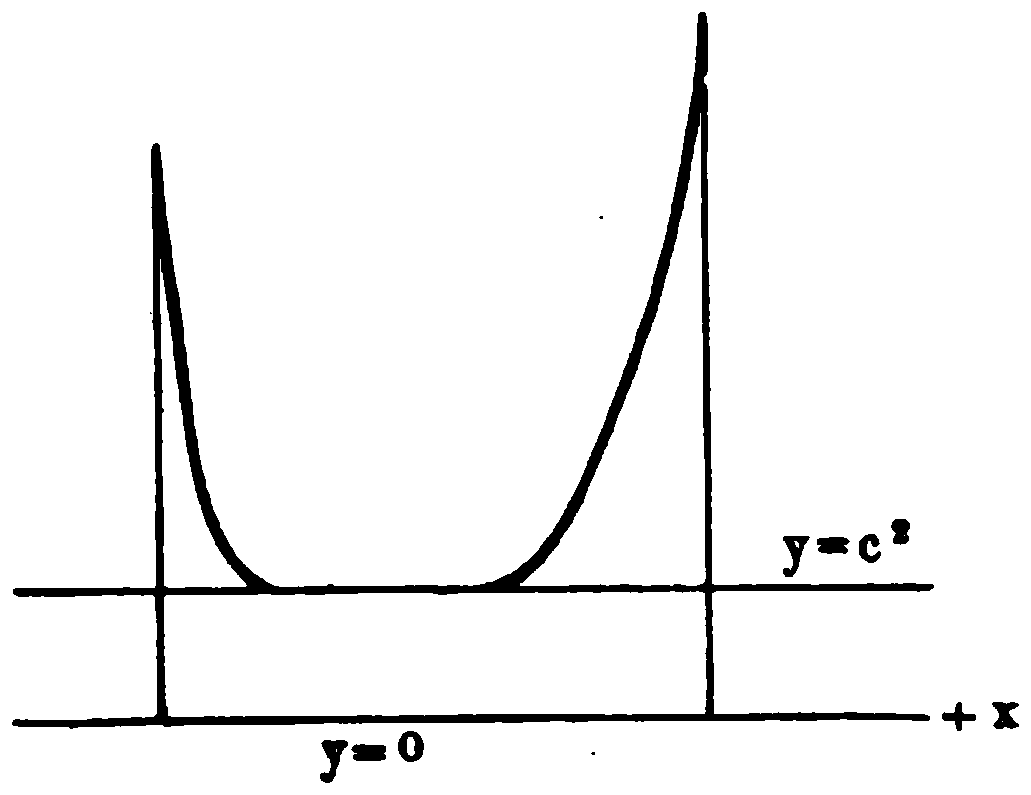
\includegraphics[width=.48\linewidth,height=42mm,keepaspectratio]{fig_assets/fig23_p0201_src_clean_x8.png}
\end{center}

Zwei Punkte der Halbebene $y>0$ können immer durch eine gebrochene Linie von der angegebenen Beschaffenheit verbunden
% src-pdfpage=0202
werden, keineswegs aber immer durch einen Bogen einer Extremale; daraus ist ersichtlich, dass die Lösung der Extremumsaufgabe durch die Einführung der gebrochenen Linie gefördert wird.

Führt man als Schranke eine Gerade $y=c^2$ ein (Fig.~23, S.~179), und ist $y-c^2$ für die gegebenen Punkte positiv, so gilt für die in der Richtung wachsender $x$ durchlaufene Schranke die Gleichung (5), während die Grösse $\mathfrak{E}$ nur in ordentlicher Weise verschwinden kann. Die gesuchte Linie muss sich also jetzt zusammensetzen aus Stücken der Geraden $y=c^2$ und sie berührenden Bögen von Kettenlinien, welche nicht in die Geraden $x=\mathrm{const.}$ degenerirt sind.

\begin{center}
{\large \S~45.}
\end{center}

Es sei, wie im vierten Abschnitt, das Integral
\[
J=\int Fdt
\]
bei vorgeschriebenem Werth des Integrals
\[
K=\int Gdt
\]
zu einem Extremum zu machen. Längs einer durch den Punkt 1 gehenden Extremale $\mathfrak{C}$ sei in der Umgebung desselben $y$ als reguläre Function von $x$ darstellbar und die Grösse
\[
F_{y'y'}+\lambda G_{y'y'}=x'^2H_1
\]
von Null verschieden; dann ist nach \S~27 die Gesammtheit aller Extremalen in der Umgebung des Punktes 1 und der Curve $\mathfrak{C}$ in der Form
\[
y=\Phi(x,a,b,\lambda)
\]
darstellbar und die Function $\Phi$ ist in der Umgebung des durch die Curve $\mathfrak{C}$ definirten Werthsystems $(x_1,a^0,b^0,\lambda^0)$ regulär. Speciell betrachten wir alle Extremalen, welche durch 1 und noch einen der Curve $\mathfrak{C}$ angehörigen Punkt 0 gehen, so dass die Gleichungen
\begin{equation}\tag{6}
y_1=\Phi(x_1,a,b,\lambda),\quad y_0=\Phi(x_0,a,b,\lambda)
\end{equation}
die Grössen $a$ und $b$ als Functionen von $\lambda$ definiren, sobald die Determinante
\[
\Psi(x_0,x_1,a^0,b^0,\lambda^0)=
\begin{vmatrix}
\Phi_a(x_1,a^0,b^0,\lambda^0)&\Phi_b(x_1,a^0,b^0,\lambda^0)\\
\Phi_a(x_0,a^0,b^0,\lambda^0)&\Phi_b(x_0,a^0,b^0,\lambda^0)
\end{vmatrix}
\]
% src-pdfpage=0203
von Null verschieden ist. Da man nun offenbar setzen kann
\[
\Phi(x,a,b,\lambda)=y_1+a+b(x-x_1)+[x-x_1]_2,
\]
so folgt
\[
\Phi_a(x,a,b,\lambda)=1+[x-x_1]_2,
\quad
\Phi_b(x,a,b,\lambda)=x-x_1+[x-x_1]_2;
\]
jene Determinante erhält also die Form
\[
\begin{vmatrix}
1&0\\
1+[x_0-x_1]_2&x_0-x_1+[x_0-x_1]_2
\end{vmatrix},
\]
und ist von Null verschieden, sobald die Grösse $|x_1-x_0|$ hinreichend klein ist. Alsdann geben die Gleichungen (6)
\[
0=\Phi_a(x_1,a,b,\lambda)\frac{da}{d\lambda}
+\Phi_b(x_1,a,b,\lambda)\frac{db}{d\lambda}
+\Phi_\lambda(x_1,a,b,\lambda),
\]
\[
0=\Phi_a(x_0,a,b,\lambda)\frac{da}{d\lambda}
+\Phi_b(x_0,a,b,\lambda)\frac{db}{d\lambda}
+\Phi_\lambda(x_0,a,b,\lambda),
\]
ausserdem hat man offenbar $\overline{K}_{01}$ als eine Function von $\lambda$ anzusehen, für welche die Gleichung
\[
\frac{d\overline{K}_{01}}{d\lambda}
=\frac{\partial\overline{K}_{01}}{\partial a}\frac{da}{d\lambda}
+\frac{\partial\overline{K}_{01}}{\partial b}\frac{db}{d\lambda}
+\frac{\partial\overline{K}_{01}}{\partial\lambda}
\]
besteht, wenn die partiellen Ableitungen in der Voraussetzung gebildet sind, dass $x_0$ und $x_1$, nicht aber $y_0$ und $y_1$ festgehalten werden. Hieraus folgt
\[
0=\begin{vmatrix}
\Phi_a(x_0,a,b,\lambda)&\Phi_b(x_0,a,b,\lambda)&\Phi_\lambda(x_0,a,b,\lambda)\\
\Phi_a(x_1,a,b,\lambda)&\Phi_b(x_1,a,b,\lambda)&\Phi_\lambda(x_1,a,b,\lambda)\\
\dfrac{\partial\overline{K}_{01}}{\partial a}&\dfrac{\partial\overline{K}_{01}}{\partial b}&\dfrac{\partial\overline{K}_{01}}{\partial\lambda}-\dfrac{d\overline{K}_{01}}{d\lambda}
\end{vmatrix}
\]
oder
\[
\Delta(x_0,x_1)=\frac{d\overline{K}_{01}}{d\lambda}\cdot\Psi(x_0,x_1,a,b,\lambda).
\]
Die linke Seite dieser Gleichung ist nach \S~42 von Null verschieden, sobald der Abstand der Punkte 0 und 1 hinreichend klein geworden ist, und
\begin{equation}\tag{7}
a=a^0,\quad b=b^0,\quad \lambda=\lambda^0
\end{equation}
gesetzt wird; dann ist die Grösse $\Psi$ endlich, und es folgt
\begin{equation}\tag{8}
0\gtrless \frac{d\overline{K}_{01}}{d\lambda}\bigg|^{a=a^0,\,b=b^0,\,\lambda=\lambda^0}.
\end{equation}
Nun ist offenbar
% src-pdfpage=0204
\[
\begin{aligned}
\frac{d\overline{K}_{01}}{d\lambda}
&=\frac{d}{d\lambda}\int_{x_0}^{x_1}g(x,y,p)\,dx \\
&=\int_{x_0}^{x_1}\left\{g_y\left(\Phi_a\frac{da}{d\lambda}+\Phi_b\frac{db}{d\lambda}+\Phi_\lambda\right)\right.\\
&\hspace{18mm}\left.+g_p\frac{d}{dx}\left(\Phi_a\frac{da}{d\lambda}+\Phi_b\frac{db}{d\lambda}+\Phi_\lambda\right)\right\}\,dx \\
&=g_p\left(\Phi_a\frac{da}{d\lambda}+\Phi_b\frac{db}{d\lambda}+\Phi_\lambda\right)\bigg|_{x_0}^{x_1}\\
&\hspace{10mm}+\int_{x_0}^{x_1}\left(g_y-\frac{dg_p}{dx}\right)
\left(\Phi_a\frac{da}{d\lambda}+\Phi_b\frac{db}{d\lambda}+\Phi_\lambda\right)\,dx \\
&=\int_{x_0}^{x_1}\left(g_y-\frac{dg_p}{dx}\right)
\left(\Phi_a\frac{da}{d\lambda}+\Phi_b\frac{db}{d\lambda}+\Phi_\lambda\right)\,dx.
\end{aligned}
\]
und ebenso
\[
\frac{d\overline{J}_{01}}{d\lambda}
=\int_{x_0}^{x_1}\left(f_y-\frac{df_p}{dx}\right)
\left(\Phi_a\frac{da}{d\lambda}+\Phi_b\frac{db}{d\lambda}+\Phi_\lambda\right)\,dx;
\]
da ferner für jede Extremale eine Gleichung
\[
f_y-\frac{df_p}{dx}+\lambda\left(g_y-\frac{dg_p}{dx}\right)=0
\]
besteht, so ergiebt sich
\begin{equation}\tag{9}
-\frac{d\overline{J}_{01}}{d\lambda}=\lambda\frac{d\overline{K}_{01}}{d\lambda},
\end{equation}
und da wir $\lambda$ als von Null verschieden voraussetzen, ist auch die linke Seite dieser Gleichung von Null verschieden bei der Annahme (7). Dabei gelten offenbar die Entwickelungen
\[
\overline{J}_{01}(\lambda)=\overline{J}_{01}(\lambda^0)+(\lambda-\lambda^0)\left(\frac{d\overline{J}_{01}}{d\lambda}\right)_{\lambda=\lambda^0}+[\lambda-\lambda^0]_2,
\]
\[
\overline{K}_{01}(\lambda)=\overline{K}_{01}(\lambda^0)+(\lambda-\lambda^0)\left(\frac{d\overline{K}_{01}}{d\lambda}\right)_{\lambda=\lambda^0}+[\lambda-\lambda^0]_2.
\]
Diese ganze Betrachtung werde für eine zweite Extremale $\mathfrak{C}_1$, auf welcher die Punkte 2 und 3 liegen, wiederholt; den zu dieser gehörigen Werth von $\lambda$ bezeichnen wir durch $\lambda_+^0$, setzen der Symmetrie halber in den bisherigen Formeln $\lambda_-$ für $\lambda$, und bezeichnen überhaupt durch die angehefteten Zeichen $-$, $+$, dass sich eine Grösse auf die Curve $\mathfrak{C}$ oder $\mathfrak{C}_1$ beziehen soll; man erhält dann die Gleichungen
% src-pdfpage=0205
\[
\overline{J}_{23}(\lambda_+)=\overline{J}_{23}(\lambda_+^0)+
(\lambda_+-\lambda_+^0)\left(\frac{d\overline{J}_{23}}{d\lambda_+}\right)_{\lambda_+=\lambda_+^0}
+[\lambda_+-\lambda_+^0]_2,
\]
\[
\overline{K}_{23}(\lambda_+)=\overline{K}_{23}(\lambda_+^0)+
(\lambda_+-\lambda_+^0)\left(\frac{d\overline{K}_{23}}{d\lambda_+}\right)_{\lambda_+=\lambda_+^0}
+[\lambda_+-\lambda_+^0]_2.
\]
Jetzt werde angenommen, die Curven $\mathfrak{C}$ und $\mathfrak{C}_1$ seien Theile eines irgendwie zusammengesetzten Linienzuges, welcher, ohne die Stetigkeitseigenschaften der in \S~2 betrachteten Curve $\mathfrak{B}$ zu haben, das Integral $J$ bei vorgeschriebenem Werth von $K$ zum Extremum macht. Dann variire man so, dass man die Bögen 23 und 01 der Curven $\mathfrak{C}_1$ und $\mathfrak{C}$ durch andere Extremalenbögen mit denselben Endpunkten ersetzt, für welche die bisherigen Bezeichnungen gelten mögen. Da das Integral $K$ längs der variirten Linie denselben Werth haben soll, wie längs der ursprünglichen, so hat man
\[
\overline{K}_{01}(\lambda_-)+\overline{K}_{23}(\lambda_+)
=\overline{K}_{01}(\lambda_-^0)+\overline{K}_{23}(\lambda_+^0),
\]
die Grössen $\lambda_-$, $\lambda_+$ sind daher durch folgende Relation verbunden:
\[
0=(\lambda_- -\lambda_-^0)\left(\frac{d\overline{K}_{01}}{d\lambda_-}\right)_{\lambda_- =\lambda_-^0}
+(\lambda_+ -\lambda_+^0)\left(\frac{d\overline{K}_{23}}{d\lambda_+}\right)_{\lambda_+ =\lambda_+^0}
+[\lambda_- -\lambda_-^0,\lambda_+ -\lambda_+^0]_2.
\]
Das Extremum erfordert, dass die Grösse
\[
\overline{J}_{01}(\lambda_-)+\overline{J}_{23}(\lambda_+)-\overline{J}_{01}(\lambda_-^0)-\overline{J}_{23}(\lambda_+^0)
\]
ein festes Vorzeichen habe. Da dieselbe in der Form
\[
(\lambda_- -\lambda_-^0)\left(\frac{d\overline{J}_{01}}{d\lambda_-}\right)_{\lambda_- =\lambda_-^0}
+(\lambda_+ -\lambda_+^0)\left(\frac{d\overline{J}_{23}}{d\lambda_+}\right)_{\lambda_+ =\lambda_+^0}
\]
\[
+[\lambda_+ -\lambda_+^0,\lambda_- -\lambda_-^0]_2
\]
dargestellt werden kann, so ergiebt der allgemeine Satz des \S~7, dass
\[
0=
\begin{vmatrix}
\dfrac{d\overline{J}_{01}}{d\lambda_-}&\dfrac{d\overline{J}_{23}}{d\lambda_+}\\[1.2ex]
\dfrac{d\overline{K}_{01}}{d\lambda_-}&\dfrac{d\overline{K}_{23}}{d\lambda_+}
\end{vmatrix}
\]
für $\lambda_- =\lambda_-^0$, $\lambda_+ =\lambda_+^0$. Hieraus folgt nach den Relationen (8), (9) und den analogen auf die Curve 23 bezüglichen
\[
0=\frac{d\overline{K}_{01}}{d\lambda_-}\frac{d\overline{K}_{23}}{d\lambda_+}
\begin{vmatrix}
\lambda_-^0&\lambda_+^0\\
1&1
\end{vmatrix},
\quad \lambda_-^0=\lambda_+^0.
\]
% src-pdfpage=0206
Diese Gleichung drückt den einfachsten Fall des von \textsc{Mayer} aufgestellten Gesetzes von der Erhaltung der isoperimetrischen Constante aus, welche nach dem erhaltenen Resultat für $\mathfrak{C}$ und $\mathfrak{C}_1$ denselben Werth hat.

\textbf{Beispiel.} Zwischen den Punkten 0 und 2 eine Linie gegebener Länge zu ziehen, welche durch den gegebenen Punkt 1 geht und mit der geraden Strecke 02 eine grösstmögliche Fläche umschliesst.

Hat die gesuchte Curve zwischen 0 und 1, sowie zwischen 1 und 2 keine Unstetigkeit, so müssen die Bögen 01 und 12 Extremalen, also Kreise sein, auf Grund der Erwägungen, die in \S~43 das entsprechende Resultat ergaben. Nach dem erhaltenen Satz besteht die gesuchte Linie nothwendig aus zwei Kreisbögen 01, 12 von gleichem Radius. Lässt man diesen variiren, so sieht man leicht, dass die Gesammtlänge der beiden Bögen innerhalb gewisser Grenzen jeden Werth annehmen kann.

% machine-unit: Kneser_LVR_DE_p0206_p0219 §§46-48
% src-pdfpage=0206
% src-break=0206
\begin{center}
{\large \S~46.}
\end{center}

Die Extremalen $\mathfrak{C}$ und $\mathfrak{C}_1$ mögen jetzt den Punkt 1 gemein haben; die Punkte 0 und 2 seien so nahe bei dem Punkte 1 angenommen, dass die durch ersteren gehenden Extremalen jeden Theil des Bogens 01, die durch letzteren gehenden jeden Theil des Bogens 12 als Feld umgeben; das ist nach \S~41 möglich, wenn $H_1$ längs der Bögen 01 und 12 nicht verschwindet (Fig.~21, S.~172). Stellt man die beiden Felder durch die Gleichungssysteme
\[
 x=\xi_-(t_-,a_-,b_-),\quad y=\eta_-(t_-,a_-,b_-),
\]
\[
 x=\xi_+(t_+,a_+,b_+),\quad y=\eta_+(t_+,a_+,b_+)
\]
dar, so kann jeder von 1 hinreichend wenig verschiedene Punkt 3 mit 0 und 2 durch Extremalen der Felder verbunden werden. Sieht man den Punkt 3 als in der Nähe der Lage 1 veränderlich an, so erhält man (\S~35)
\begin{equation}\tag{10}
\frac{\partial\overline K_{03}}{\partial t_-}=G_-\bigg|^3,
\quad
\frac{\partial\overline K_{03}}{\partial a_-}
=\int_0^3\bigl[\xi_a(G_x-G_{x'}')+\eta_a(G_y-G_{y'}')\bigr]_-\,dt_-
+\bigl(\xi_aG_{x'}+\eta_aG_{y'}\bigr)_-\bigg|^3
\end{equation}
nebst einer analogen Formel, in welcher $a$ durch $b$ ersetzt ist; wenn daher dem Uebergang vom Punkte 1 zu 3 und vom Bogen 01 zu 03 die Incremente $\delta t_-$, $\delta a_-$, $\delta b_-$ entsprechen, so ist
% src-pdfpage=0207
\[
\overline K_{03}-\overline K_{01}=\Delta\overline K_{01}
=G_{x'}^-\delta x+G_{y'}^-\delta y\bigg|^1
+A_-\delta a_-+B_-\delta b_-+[\delta t_-,\delta a_-,\delta b_-]_2,
\]
wobei gesetzt ist
\begin{equation}\tag{11}
\delta x=(\xi_a\delta a+\xi_b\delta b+\xi_t\delta t)_-,
\quad
\delta y=(\eta_a\delta a+\eta_b\delta b+\eta_t\delta t)_-,
\end{equation}
\[
A_- =\int_0^1\bigl[\xi_a(G_x-G_{x'}')+\eta_a(G_y-G_{y'}')\bigr]_-\,dt_-
\]
und $B_-$ aus $A_-$ entsteht, indem man $a$ durch $b$ ersetzt. Analog ergiebt sich
\[
\Delta\overline K_{12}
=-G_{x'}^+\delta x-G_{y'}^+\delta y\bigg|^1
+A_+\delta a_+ +B_+\delta b_+ +[\delta t_+,\delta a_+,\delta b_+]_2,
\]
wobei die Grössen $\delta t_+$, $\delta a_+$, $\delta b_+$, $A_+$, $\ldots$ für die Extremale 12 die analoge Bedeutung haben wie $\delta t_-$, $\ldots$ für 01, so dass
\begin{equation}\tag{12}
\delta x=(\xi_a\delta a+\xi_b\delta b+\xi_t\delta t)_+,
\quad
\delta y=(\eta_a\delta a+\eta_b\delta b+\eta_t\delta t)_+.
\end{equation}
Soll nun $J$ bei gegebenem Werthe von $K$ ein Extremum werden, so ist die aus den Extremalenbögen 03, 32 bestehende gebrochene Linie eine erlaubte Variation der gebrochenen Linie 012, sobald man die acht Grössen $\delta x$, $\delta y$, $\delta a_\pm$, $\delta b_\pm$, $\delta t_\pm$ so bestimmt, dass die Gleichung
\[
\Delta\overline K_{01}+\Delta\overline K_{12}=0
\]
besteht, oder
\begin{equation}\tag{13}
\begin{aligned}
0={}&(G_{x'}^- -G_{x'}^+)\delta x+(G_{y'}^- -G_{y'}^+)\delta y\bigg|^1 \\
&+A_-\delta a_-+B_-\delta b_-+A_+\delta a_+ +B_+\delta b_+ \\
&+[\delta a_+,\delta b_+,\delta t_+,\delta a_-,\delta b_-,\delta t_-]_2.
\end{aligned}
\end{equation}
Diese Gleichung in Verbindung mit den unter (11) und (12) angeführten kann dazu dienen, fünf der acht Grössen $\delta$ durch die drei übrigen auszudrücken. Nimmt man für letztere z.~B. $\delta x$, $\delta y$, $\delta a_+$, so ist die Determinante der in den Grössen $\delta t_-$, $\delta a_-$, $\delta b_-$, $\delta t_+$, $\delta b_+$ linearen Glieder auf den rechten Seiten der bezeichneten fünf Gleichungen
% src-pdfpage=0208
\begin{equation}\tag{14}
\begin{vmatrix}
0&A_-&B_-&0&B_+\\
\xi_t^-&\xi_a^-&\xi_b^-&0&0\\
\eta_t^-&\eta_a^-&\eta_b^-&0&0\\
0&0&0&\xi_t^+&\xi_b^+\\
0&0&0&\eta_t^+&\eta_b^+
\end{vmatrix}
=
\begin{vmatrix}
0&A_-&B_-\\
\xi_t^-&\xi_a^-&\xi_b^-\\
\eta_t^-&\eta_a^-&\eta_b^-
\end{vmatrix}
\left[\frac{\partial(\xi,\eta)}{\partial(t,b)}\right]_+ .
\end{equation}
Addirt man in der ersten Determinante rechts die zweite und dritte Horizontalreihe, mit $G_{x'}^-$ und $G_{y'}^-$ multiplicirt, zur ersten, und bedenkt, dass die Ableitungen von $\xi$ und $\eta$ sich wie in den Gleichungen (11) auf den Punkt 1 beziehen, so zeigen die Gleichungen (10), dass die Determinante den Werth
\[
\frac{\partial(\overline K_{01},\xi_-,\eta_-)}{\partial(t_-,a_-,b_-)}
\]
hat, d.~h. der auf das Feld des Bogens 01 bezüglichen Grösse $\Delta_-$ gleich, also von Null verschieden ist. Da ferner auch der Bogen 12 mit einem Felde umgeben ist, für welches die Grösse
\[
\frac{\partial(\xi_+,\eta_+,\overline K_{21})}{\partial(t_+,a_+,b_+)}
\]
nicht verschwindet, so sind nach \S~35 die Grössen
\[
\left[\frac{\partial(\xi,\eta)}{\partial(t,a)}\right]_+,
\quad
\left[\frac{\partial(\xi,\eta)}{\partial(t,b)}\right]_+
\]
nicht beide gleich Null; entweder also ist auch der zweite Factor auf der rechten Seite der Gleichung (14) von Null verschieden, oder man erreicht dies, indem man $a_+$ und $b_+$ vertauscht. Man kann also stets fünf der Grössen $\delta$ durch die drei übrigen, unter welchen $\delta x$ und $\delta y$ vorkommen, als Potenzreihen dieser drei Argumente ausdrücken.

Ersetzt man nun in den Ausdrücken $A$, $B$ das Functionszeichen $G$ durch $F$, so erhalte man $\mathfrak A$, $\mathfrak B$; die Gleichung der Extremalen liefert dann
\begin{equation}\tag{15}
\lambda_-A_-+\mathfrak A_-=
\lambda_-B_-+\mathfrak B_-=
\lambda_+A_+ +\mathfrak A_+=
\lambda_+B_+ +\mathfrak B_+=0,
\end{equation}
und nach dem vorigen Paragraphen hat man für $\mathfrak C$ und $\mathfrak C_1$
\[
\lambda_+=\lambda_-=\lambda.
\]
Dem in der Gleichung (13) entwickelten Ausdruck $\Delta\overline K_{01}+\Delta\overline K_{12}$ analog erhält man ferner
% src-pdfpage=0209
\[
\begin{aligned}
\Delta\overline J_{01}+\Delta\overline J_{12}
={}&(F_{x'}^- -F_{x'}^+)\delta x+(F_{y'}^- -F_{y'}^+)\delta y\bigg|^1\\
&+\mathfrak A_-\delta a_-+\mathfrak B_-\delta b_-+\mathfrak A_+\delta a_+ +\mathfrak B_+\delta b_+ \\
&+[\delta a_\pm,\delta b_\pm,\delta t_\pm]_2;
\end{aligned}
\]
multiplicirt man daher die Gleichung (13) mit $\lambda$ und addirt sie zu der letzten, so ergiebt sich, da $H=F+\lambda G$, nach (15)
\[
\Delta\overline J_{01}+\Delta\overline J_{12}
=(H_{x'}^- -H_{x'}^+)\delta x+(H_{y'}^- -H_{y'}^+)\delta y\bigg|^1
+[\delta a_\pm,\delta b_\pm,\delta t_\pm]_2.
\]
Diese Grösse muss, wenn das verlangte Extremum vorliegt, bei den Bedingungen (11), (12), (13) ein festes Vorzeichen haben; da hier nur die Grössen $\delta x$, $\delta y$ in den linearen Gliedern vorkommen, ergiebt sich nach \S~7 für den Punkt 1
\begin{equation}\tag{16}
(H_{x'}^- -H_{x'}^+)\delta x+(H_{y'}^- -H_{y'}^+)\delta y=0.
\end{equation}
Je nachdem also der Punkt 1 frei beweglich oder an die Curve
\[
h(x,y)=0
\]
gebunden ist, erhält man die Relationen
\[
H_{x'}^- -H_{x'}^+=H_{y'}^- -H_{y'}^+=0
\]
oder
\[
\begin{vmatrix}
H_{x'}^- -H_{x'}^+&H_{y'}^- -H_{y'}^+\\
h_x&h_y
\end{vmatrix}=0.
\]
Es gelten daher für einen Eckpunkt genau dieselben Beschränkungen wie nach \S~43 im Falle des absoluten Extremums, wenn man $F$ durch $F+\lambda G$ ersetzt.

\textbf{Beispiel. Aufgabe IX} (\S~34). Man hat
\[
H=yx' +\lambda\sqrt{x'^2+y'^2},
\]
\[
H_{x'}=y+\frac{\lambda x'}{\sqrt{x'^2+y'^2}},
\quad
H_{y'}=\frac{\lambda y'}{\sqrt{x'^2+y'^2}};
\]
die Gleichung (16) ergiebt also
\begin{equation}\tag{17}
\lambda\left(\frac{x'\delta x+y'\delta y}{\sqrt{x'^2+y'^2}}\right)_-
=
\lambda\left(\frac{x'\delta x+y'\delta y}{\sqrt{x'^2+y'^2}}\right)_+.
\end{equation}
Da nun $\lambda$ von Null verschieden ist, so würde für eine frei verfügbare Ecke folgen
\[
\left(\frac{x'}{\sqrt{x'^2+y'^2}}\right)_-
=
\left(\frac{x'}{\sqrt{x'^2+y'^2}}\right)_+,
\quad
\left(\frac{y'}{\sqrt{x'^2+y'^2}}\right)_-
=
\left(\frac{y'}{\sqrt{x'^2+y'^2}}\right)_+,
\]
% src-pdfpage=0210
 d.~h. die Richtungen der Extremalen 01 und 12 würden im Punkte 1 übereinstimmen, eine Unstetigkeit also nicht eintreten. Ist dagegen der Punkt 1 an eine Curve $\mathfrak K$ gebunden, deren Bogenelement $Ds$ sei, und bezeichnen wir im Punkte 1 durch $-$, $+$ die Richtungen der Extremale 01 von 0 nach 1 hin und der Extremale 12 von 1 nach 2 hin, so ergiebt die Gleichung (17)
\[
\cos(Ds,-)=\cos(Ds,+).
\]
Die Bögen 01 und 12 liegen daher auf derselben Seite der Curve $\mathfrak K$ und bilden mit deren Tangente gleiche, nach verschiedenen Seiten geöffnete spitze Winkel, d.~h. sie liegen wie der einfallende und reflectirte Lichtstrahl.

Soll z.~B. vom gegebenen Punkte 5 aus nach einem nicht vorgeschriebenen Punkte 1 der Curve $\mathfrak K$ und wieder zum Punkte 5 zurück eine geschlossene Linie von gegebener Länge gezogen werden, die eine möglichst grosse Fläche umfasst, so muss sie aus zwei Kreisbögen von gleichem Radius bestehen, welche mit der Curve $\mathfrak K$ im angegebenen Sinne gleiche Winkel bilden.

\begin{center}
{\large \S~47.}
\end{center}

Es bleibt noch zu untersuchen, wann ein Linienzug 0123 bei der Lösung des isoperimetrischen Problems auftreten kann, wenn die verglichenen Curven an ein von Schranken begrenztes Gebiet $\mathfrak G$ gebunden sind, und die Strecke 12 einer Schranke angehört, die Bögen 01 und 23 aber nicht, so dass letztere nach \S~45 Extremalen mit derselben isoperimetrischen Constante sind. Dann seien (Fig.~24) die Punkte 0 und 3 so nahe bei 1 und 2 angenommen, dass die Bögen 01 und 23 mit Feldern umgeben werden können, deren Extremalen durch 0 und 3 gehen. In der Nähe der Punkte 1 und 2 seien auf der Schranke die Punkte 4 und 5 gelegen; dann giebt es Extremalen 04 und 53, welche den beiden Feldern angehören, und der Linienzug 0453 ist eine erlaubte Variation des Zuges 0123, wenn
\[
\overline K_{01}+K_{12}+\overline K_{23}=\overline K_{04}+K_{45}+\overline K_{53},
\]
oder
\begin{equation}\tag{18}
K_{12}-K_{45}=\Delta\overline K_{01}+\Delta\overline K_{23},
\end{equation}
\begin{center}
{\small Fig. 24.}\par\vspace{1mm}
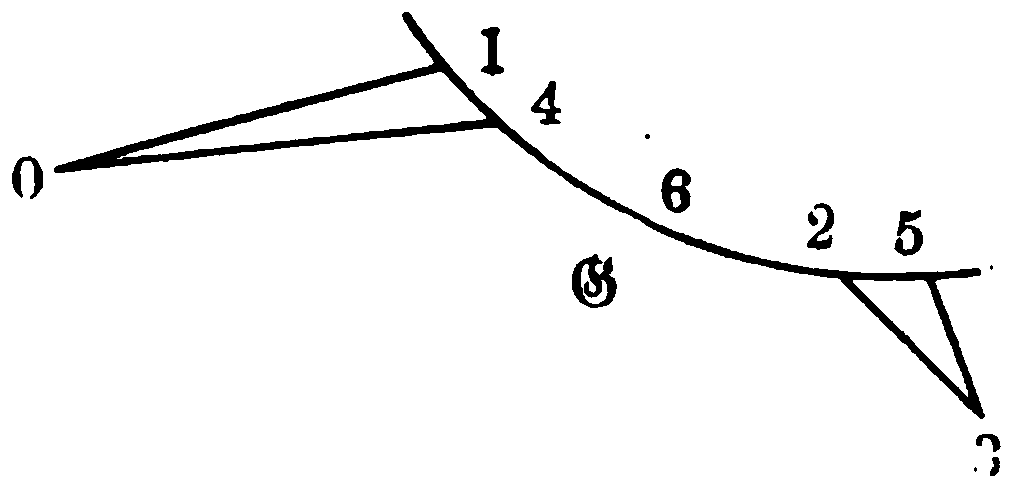
\includegraphics[width=.48\linewidth,height=42mm,keepaspectratio]{fig_assets/fig24_p0210_src_clean_x8.png}
\end{center}
% src-pdfpage=0211
wobei sich die ungestrichenen Integrale stets auf die Schranke beziehen und die Zeichen $\Delta$ den Zuwachs beim Uebergang von 01 und 23 zu 04 und 53 bedeuten. Um diese Forderung zu discutiren, legen wir den Zeichen $\xi$, $\eta$, $t_+$, $a_\pm$, $b_\pm$, $A_\pm$, $\delta t_\pm\ldots$ dieselbe Bedeutung für die Bögen 01 und 23 bei, die sie im vorigen Paragraphen für 01 und 12 hatten, so dass das Zeichen $-$ dem ersten, das Zeichen $+$ dem zweiten der bezeichneten Bögen zugehört; demgemäss sei
\[
\begin{aligned}
\delta x_-+[\delta t_-,\delta a_-,\delta b_-]_2&=x_4-x_1,\\
\delta y_-+[\delta t_-,\delta a_-,\delta b_-]_2&=y_4-y_1,\\
\delta x_++[\delta t_+,\delta a_+,\delta b_+]_2&=x_5-x_2,\\
\delta y_++[\delta t_+,\delta a_+,\delta b_+]_2&=y_5-y_2,
\end{aligned}
\]
und die Ausdrücke $\delta x$, $\delta y$ in Bezug auf $\delta t$, $\delta a$, $\delta b$ linear. Die rechte Seite der Gleichung (18) findet man dann aus den im \S~46 für $K_{01}$ aufgestellten Formeln; man hat nämlich
\begin{equation}\tag{19}
\begin{aligned}
\Delta\overline K_{01}&=G_{x'}^-\delta x_-+G_{y'}^-\delta y_-\bigg|^1
+A_-\delta a_-+B_-\delta b_-+[\delta t_-,\delta a_-,\delta b_-]_2,\\
\Delta\overline K_{23}&=-G_{x'}^+\delta x_+ -G_{y'}^+\delta y_+\bigg|^2
+A_+\delta a_+ +B_+\delta b_+ +[\delta t_+,\delta a_+,\delta b_+]_2;
\end{aligned}
\end{equation}
und es bestehen zwischen den Grössen $\delta$ jetzt die vier Relationen
\begin{equation}\tag{20}
\delta x_\pm=(\xi_t\delta t+\xi_a\delta a+\xi_b\delta b)_\pm,
\quad
\delta y_\pm=(\eta_t\delta t+\eta_a\delta a+\eta_b\delta b)_\pm,
\end{equation}
wobei entweder auf beiden Seiten das obere, oder auf beiden das untere der Zeichen $\pm$ zu nehmen ist. Sieht man daher hier und in der Gleichung (18) die Grössen $\delta t_-$, $\delta a_-$, $\delta b_-$, $\delta b_+$, $\delta t_+$ als bestimmt durch die übrigen Grössen $\delta$ an, so haben die jene fünf Grössen enthaltenden Glieder in den angesetzten fünf Gleichungen genau dieselbe Determinante wie in den Gleichungen (11), (12), (13) des vorigen Paragraphen. Der dort gegebene Beweis dafür, dass diese Determinante oder die durch Vertauschung von $a_+$ und $b_+$ erhaltene von Null verschieden ist, bleibt gültig, wenn man den dort betrachteten Bogen 12 durch 23 ersetzt. Die fünf Gleichungen (18), (20) können daher nach den Grössen $\delta t_\pm$, $\delta a_-$, $\delta b_\pm$ aufgelöst werden, sobald $K_{12}-K_{45}$ hinreichend klein ist.

% src-pdfpage=0212
Jetzt seien $x$ und $y$ längs der Schranke in der Nähe der Punkte 1 und 2 reguläre Functionen der Parameter $\tau_-$, $\tau_+$, welche in der Richtung 12 wachsen und beim Uebergang zu 4 und 5 die Incremente $D\tau_-$ und $D\tau_+$ erhalten mögen; dann ist
\[
\delta x_- =\frac{dx}{d\tau_-}\bigg|^1D\tau_-+[D\tau_-]_2,
\quad
\delta y_- =\frac{dy}{d\tau_-}\bigg|^1D\tau_-+[D\tau_-]_2,
\]
und ähnliche Gleichungen bestehen im Punkte 2. Setzt man noch voraus, dass die Integranden $F$ und $G$ in der Umgebung jedes Elementes des Zuges 0123 regulär seien, so ist bei positiven Werthen $D\tau_-$
\begin{equation}\tag{21}
K_{14}=G\left(x,y,\frac{dx}{d\tau_-},\frac{dy}{d\tau_-}\right)\bigg|^1D\tau_-+[D\tau_-]_2,
\end{equation}
bei negativen
\begin{equation}\tag{22}
K_{41}=G\left(x,y,\frac{dx}{d\tau_-},\frac{dy}{d\tau_-}\right)\bigg|^1(-D\tau_-)+[D\tau_-]_2.
\end{equation}
Wenn nun auf der Schranke der Punkt 6 zwischen 1 und 2 und ausserhalb der Strecken 14, 25 beliebig fixirt wird, so hat man, je nachdem $D\tau_-$ positiv oder negativ ist, die eine oder andere der Gleichungen
\[
K_{46}-K_{16}=-K_{14},
\quad
K_{46}-K_{16}=K_{41};
\]
in jedem Falle also nach (21), (22)
\begin{equation}\tag{23}
\Delta K_{16}=K_{46}-K_{16}
=-G\left(x,y,\frac{dx}{d\tau_-},\frac{dy}{d\tau_-}\right)\bigg|^1D\tau_-+[D\tau_-]_2.
\end{equation}
Auf ähnliche Weise ergiebt sich
\begin{equation}\tag{24}
\Delta K_{62}=K_{65}-K_{62}
=+G\left(x,y,\frac{dx}{d\tau_+},\frac{dy}{d\tau_+}\right)\bigg|^2D\tau_+ +[D\tau_+]_2;
\end{equation}
setzt man die Summe dieser Ausdrücke
\[
\Delta K_{16}+\Delta K_{62}=\Delta K_{12}=K_{45}-K_{12}
\]
in die Gleichung (18), so folgt nach (19)
\begin{equation}\tag{25}
\begin{aligned}
&G\left(x,y,\frac{dx}{d\tau_-},\frac{dy}{d\tau_-}\right)\bigg|^1D\tau_-
-G\left(x,y,\frac{dx}{d\tau_+},\frac{dy}{d\tau_+}\right)\bigg|^2D\tau_+\\
&\quad=G_{x'}^-\frac{dx}{d\tau_-}+G_{y'}^-\frac{dy}{d\tau_-}\bigg|^1D\tau_-
-G_{x'}^+\frac{dx}{d\tau_+}-G_{y'}^+\frac{dy}{d\tau_+}\bigg|^2D\tau_+\\
&\qquad +A_-\delta a_-+B_-\delta b_-+A_+\delta a_+ +B_+\delta b_+
+[\delta a_\pm,\delta b_\pm,\delta t_\pm,D\tau_\pm]_2.
\end{aligned}
\end{equation}

% src-pdfpage=0213
Die rechten Seiten der Gleichungen (19) gehen in $\Delta\overline J_{01}$ und $\Delta\overline J_{23}$ über, wenn man $G$ durch $F$, $A$ und $B$ durch $\mathfrak A$ und $\mathfrak B$ ersetzt; multiplicirt man daher die letzte Gleichung mit der zu beiden Curven 01 und 23 gehörigen Constante $\lambda$, und berücksichtigt die Gleichungen (15), so ergiebt sich
\[
\begin{aligned}
&\Delta\overline J_{01}+\Delta\overline J_{23}
+\lambda G\left(x,y,\frac{dx}{d\tau_-},\frac{dy}{d\tau_-}\right)\bigg|^1D\tau_-\\
&\quad -\lambda G\left(x,y,\frac{dx}{d\tau_+},\frac{dy}{d\tau_+}\right)\bigg|^2D\tau_+\\
&=H_{x'}^-\frac{dx}{d\tau_-}+H_{y'}^-\frac{dy}{d\tau_-}\bigg|^1D\tau_-
-H_{x'}^+\frac{dx}{d\tau_+}-H_{y'}^+\frac{dy}{d\tau_+}\bigg|^2D\tau_+\\
&\quad +[\delta a_\pm,\delta b_\pm,\delta t_\pm,D\tau_\pm]_2.
\end{aligned}
\]
Nun erhält das Integral $J_{0123}$ bei der betrachteten Variation den Zuwachs
\[
\Delta\overline J_{01}+\Delta\overline J_{23}+J_{45}-J_{12}
=\Delta\overline J_{01}+\Delta\overline J_{23}+\Delta J_{16}+\Delta J_{62};
\]
da ferner analog den Gleichungen (23), (24) gesetzt werden kann
\[
\Delta J_{16}=-F\left(x,y,\frac{dx}{d\tau_-},\frac{dy}{d\tau_-}\right)\bigg|^1D\tau_-+[D\tau_-]_2,
\]
\[
\Delta J_{62}=F\left(x,y,\frac{dx}{d\tau_+},\frac{dy}{d\tau_+}\right)\bigg|^2D\tau_+ +[D\tau_+]_2,
\]
so erhält man für jenen Zuwachs den Ausdruck
\[
\begin{aligned}
&H_{x'}^-\frac{dx}{d\tau_-}+H_{y'}^-\frac{dy}{d\tau_-}
-H\left(x,y,\frac{dx}{d\tau_-},\frac{dy}{d\tau_-}\right)\bigg|^1D\tau_-\\
&\quad -H_{x'}^+\frac{dx}{d\tau_+}-H_{y'}^+\frac{dy}{d\tau_+}
+H\left(x,y,\frac{dx}{d\tau_+},\frac{dy}{d\tau_+}\right)\bigg|^2D\tau_+\\
&\quad +[\delta t_\pm,\delta a_\pm,\delta b_\pm,D\tau_\pm]_2,
\end{aligned}
\]
oder kurz
\[
\Delta J_{0123}=\mathfrak E^-D\tau_- -\mathfrak E^+D\tau_+ +[\delta t_\pm,\delta a_\pm,\delta b_\pm,D\tau_\pm]_2,
\]
wobei die Grösse $\mathfrak E^-$ für das vom Punkte 1 ausgehende über ihn hinausführende Element der Extremale 01 und das den wachsenden Werthen von $\tau_-$ entsprechende Element der Schranke und $\mathfrak E^+$ im Punkte 2 für das nach 3 hinweisende Element der Extremale und die Richtung wachsender $\tau_+$ gebildet ist.

Soll das verlangte Extremum vorliegen, so muss $\Delta J_{0123}$ ein festes Vorzeichen haben bei allen den Relationen (20), (25) unterworfenen Grössen $\delta$, $D$. Unter diesen bleiben $D\tau_+$ und $D\tau_-$ frei verfügbar; der Satz des \S~7 ergiebt also, dass der lineare Theil
% src-pdfpage=0214
von $\Delta J_{0123}$, welcher keine der durch jene Relationen bestimmten Variationen enthält, bei beliebigen Werthen von $D\tau_-$ und $D\tau_+$ verschwindet, d.~h.
\[
\mathfrak E^- = \mathfrak E^+=0.
\]
Ist daher ausserordentliches Verschwinden der Grösse $\mathfrak E$ in den Punkten 1 und 2 ausgeschlossen, so muss in diesen die Schranke von den an sie stossenden Extremalen berührt werden, so dass auch hier das für absolute Extrema bewiesene Resultat erhalten bleibt.

\textbf{Beispiele. Aufgabe IX.} Die Grösse $\mathfrak E$ kann nach \S~37 nur in ordentlicher Weise verschwinden; soll daher z.~B. innerhalb eines ebenen Polygons eine geschlossene Linie von gegebener Länge und grösstmöglichem Inhalt gezogen werden, und hat eine Kreislinie von der vorgeschriebenen Länge innerhalb des Polygons nicht Platz, so kann die gesuchte Linie nur aus Theilen der Polygonseiten und diese berührenden Kreisbögen von gleichem Radius bestehen.

\textbf{Aufgabe X.} Die Grösse $\mathfrak E$ verschwindet, da sie sich in der Bezeichnung des \S~34 von der bei der Aufgabe IX auftretenden nur um den Factor $\sqrt M$ unterscheidet, nur in ordentlicher Weise, so lange $M$ von Null verschieden bleibt. Gilt dies für ein Gebiet, welches von regulären Curvenstücken begrenzt ist, und soll innerhalb desselben eine geschlossene Linie gegebenen Inhaltes und kleinstmöglicher Länge gezogen werden, so kann dieselbe nur aus Theilen der umschränkenden Curvenstücke und Bögen constanter geodätischer Krümmung bestehen, welch letztere alle dieselbe Grösse der geodätischen Krümmung aufweisen, und die Schranke, wo sie mit ihr zusammentreffen, berühren. Dieser Satz ist von \textsc{Steiner} aufgestellt worden.

% src-pdfpage=0215
\begin{center}
{\large Sechster Abschnitt.}\par
\vspace{2mm}
{\Large\bfseries Das Extremum der Integrale, welche höhere\\ Ableitungen der Unbekannten enthalten.}\par
\vspace{2mm}\rule{32mm}{0.4pt}\par
\vspace{2mm}
{\large \S~48.}
\end{center}

Es sei $\mathfrak B$ ein Stück einer ebenen Curve, längs dessen $x$ und $y$ als stetige Functionen eines Parameters $t$ darstellbar, und ihre Ableitungen bis zur $n^{\mathrm{ten}}$ Ordnung einschliesslich ebenfalls stetige Functionen von $t$ sind. Die Function
\[
F(x,x',x'',\ldots x^{(n)},y,y',y'',\ldots y^{(n)})
\]
sei für jedes durch ein Element des Bogens $\mathfrak B$ definirte Werthsystem ihrer Argumente regulär, und von den Grössen $x'$, $y'$ sei an jeder Stelle des Bogens mindestens eine von Null verschieden. Wir betrachten nur solche Integrale
\[
J=\int Fdt,
\]
deren Werth durch die Curve $\mathfrak B$ allein bestimmt ist, nicht aber von der speciellen Natur des Zusammenhanges zwischen $x$, $y$ und $t$ abhängt. Sind dann $x$ und $y$ längs des Bogens $\mathfrak B$ Functionen des Parameters $\theta$, welche dieselben Eigenschaften haben, wie die vorher eingeführten des Parameters $t$, und sind 0 und 1 irgend zwei Punkte des Bogens $\mathfrak B$, so muss die Gleichung
\[
J_{01}=\int_0^1 F(x,x',\ldots,y^{(n)})\,dt
=\int_0^1 F\left(x,\frac{dx}{d\theta},\ldots,\frac{d^ny}{d\theta^n}\right)d\theta
\]
bestehen. Die Werthe der Variablen $t$ und $\theta$ werden durch die Punkte der Curve einander zugeordnet, so dass z.~B. $\theta$ als Function von $t$ angesehen werden kann; lässt man die obere Grenze des Integrals sich ändern, und differenzirt nach dem zu ihr
% src-pdfpage=0216
gehörigen Werthe von $t$, so ergiebt sich
\[
F(x,x',\ldots y^{(n)})
=F\left(x,\frac{dx}{d\theta},\ldots,\frac{d^ny}{d\theta^n}\right)\frac{d\theta}{dt},
\]
oder
\begin{equation}\tag{1}
F\left(x,\frac{dx}{dt},\ldots,\frac{d^ny}{dt^n}\right)dt
=F\left(x,\frac{dx}{d\theta},\ldots,\frac{d^ny}{d\theta^n}\right)d\theta.
\end{equation}
Speciell kann an einer Stelle, für welche $x'$ nicht verschwindet, $\theta=x$ gesetzt, d.~h. $y$ als Function von $x$ betrachtet werden, deren Ableitungen bis zur $n^{\mathrm{ten}}$ Ordnung als ganze Functionen von $x$, $x'$, $\ldots x^{(n)}$, $y$, $y'$, $\ldots y^{(n)}$, dividirt durch Potenzen von $x'$, darstellbar, also stetige Functionen von $x$ sind. Da nun
\[
\frac{dx}{d\theta}=1,
\quad
\frac{d^2x}{d\theta^2}=\cdots=\frac{d^nx}{d\theta^n}=0,
\]
so hat man der Gleichung (1) zufolge
\[
F(x,x',\ldots y^{(n)})dt
=F\left(x,1,0,\ldots,0,y,\frac{dy}{dx},\ldots,\frac{d^ny}{dx^n}\right)dx
\]
oder in neuer Bezeichnung
\[
F(x,x',\ldots y^{(n)})dt
=f\left(x,y,\frac{dy}{dx},\ldots,\frac{d^ny}{dx^n}\right)dx,
\quad J=\int fdx.
\]
Eine beliebige Darstellung des Bogens $\mathfrak B$ von den angegebenen Eigenschaften sei durch die Gleichungen
\begin{equation}\tag{2}
x=\varphi(\theta),\quad y=\psi(\theta)
\end{equation}
gegeben; dann erhält man eine andere Darstellung, wenn man $\theta=t+\tau$ setzt, und unter $\tau$ eine beliebige Function von $t$ versteht, welche in gewissen Constanten $\varepsilon$ homogen linear sei. Es gelten dann offenbar die Gleichungen
\[
x=\varphi(t+\tau),\quad y=\psi(t+\tau),
\]
und die \textsc{Taylor}'schen Entwickelungen
\[
x=\varphi(t)+\varphi'(t)\tau+\cdots,
\quad x-\varphi(t)=\varphi'(t)\tau+\cdots,
\]
\[
y=\psi(t)+\psi'(t)\tau+\cdots,
\quad y-\psi(t)=\psi'(t)\tau+\cdots;
\]
aus diesen folgt
\[
\frac{d^\alpha x}{dt^\alpha}-\varphi^{(\alpha)}(t)
=\frac{d^\alpha[\varphi'(t)\tau]}{dt^\alpha}+\cdots,
\quad
\frac{d^\alpha y}{dt^\alpha}-\psi^{(\alpha)}(t)
=\frac{d^\alpha[\psi'(t)\tau]}{dt^\alpha}+\cdots,
\]
wobei die weggelassenen Glieder in Bezug auf $\tau$ und die Ableitungen dieser Grösse von mindestens zweiter Dimension sind,
% src-pdfpage=0217
mithin auch die Grössen $\varepsilon$ in derselben Weise enthalten. Andererseits ist offenbar
\[
\frac{d^\alpha x}{d\theta^\alpha}=\varphi^{(\alpha)}(\theta)=\varphi^{(\alpha)}(t+\tau),
\quad
\frac{d^\alpha y}{d\theta^\alpha}=\psi^{(\alpha)}(\theta)=\psi^{(\alpha)}(t+\tau);
\]
die Gleichung (1) ergiebt also
\[
F[\varphi(t+\tau),\varphi'(t+\tau),\ldots]\left(1+\frac{d\tau}{dt}\right)
\]
\[
=F\left(\varphi(t)+\tau\varphi'(t)+[\varepsilon]_2,
\varphi'(t)+\frac{d[\tau\varphi'(t)]}{dt}+[\varepsilon]_2,
\varphi''(t)+\frac{d^2[\tau\varphi'(t)]}{dt^2}+[\varepsilon]_2,\ldots\right),
\]
oder, indem man links nach Potenzen von $\tau$, rechts nach Potenzen der die Grössen $\varepsilon$ enthaltenden Theile der Argumente entwickelt, und durch das Suffix $\varphi\psi$ andeutet, dass
\[
x=\varphi(t),\quad x'=\varphi'(t),\ldots,
\quad y=\psi(t),\quad y'=\psi'(t),\ldots
\]
zu setzen ist,
\[
\left(F_{\varphi\psi}+\tau\frac{dF_{\varphi\psi}}{dt}+[\varepsilon]_2\right)\left(1+\frac{d\tau}{dt}\right)
\]
\[
=F_{\varphi\psi}+\sum_{a=0}^n\left\{\left(\frac{\partial F}{\partial x^{(a)}}\right)_{\varphi\psi}\frac{d^a[\tau\varphi'(t)]}{dt^a}
+\left(\frac{\partial F}{\partial y^{(a)}}\right)_{\varphi\psi}\frac{d^a[\tau\psi'(t)]}{dt^a}\right\}+[\varepsilon]_2.
\]
Behält man daher nur die Glieder bei, die in den Constanten $\varepsilon$ linear sind, so ergiebt sich
\[
\tau\frac{dF_{\varphi\psi}}{dt}+F_{\varphi\psi}\frac{d\tau}{dt}
=\frac{d(F_{\varphi\psi}\tau)}{dt}
\]
\[
=\sum_{a=0}^n\left\{\left(\frac{\partial F}{\partial x^{(a)}}\right)_{\varphi\psi}\frac{d^a[\tau\varphi'(t)]}{dt^a}
+\left(\frac{\partial F}{\partial y^{(a)}}\right)_{\varphi\psi}\frac{d^a[\tau\psi'(t)]}{dt^a}\right\},
\]
oder, wenn man jetzt den Bogen $\mathfrak B$ durch die mit den Gleichungen (2) gleichwerthigen
\[
x=\varphi(t),\quad y=\psi(t)
\]
darstellt, und durch Accente, wie immer, die Differentiation nach $t$ bezeichnet,
\[
(F\tau)'=\sum_{a=0}^n\left\{\frac{\partial F}{\partial x^{(a)}}(x'\tau)^{(a)}+\frac{\partial F}{\partial y^{(a)}}(y'\tau)^{(a)}\right\},
\]
oder endlich mit unbestimmtem Integralzeichen
\begin{equation}\tag{3}
F\tau=\int dt\sum_{a=0}^n\left\{\frac{\partial F}{\partial x^{(a)}}(x'\tau)^{(a)}+\frac{\partial F}{\partial y^{(a)}}(y'\tau)^{(a)}\right\}.
\end{equation}

% src-pdfpage=0218
Die rechte Seite dieser Gleichung transformiren wir mittelst der Identität
\[
\int vu^{(a)}dt=vu^{(a-1)}-v'u^{(a-2)}+v''u^{(a-3)}-\cdots
+(-1)^{a-1}v^{(a-1)}u+(-1)^a\int v^{(a)}u\,dt,
\]
deren Richtigkeit, wenn $u$ und $v$ beliebige Functionen von $t$ sind, offenbar wird, wenn man beide Seiten nach $t$ differenzirt. Setzt man speciell
\[
v=\frac{\partial F}{\partial x^{(a)}},\quad u=x'\tau,
\]
so ergiebt sich
\[
\int\frac{\partial F}{\partial x^{(a)}}(x'\tau)^{(a)}dt
=\frac{\partial F}{\partial x^{(a)}}(x'\tau)^{(a-1)}
-\frac{d}{dt}\frac{\partial F}{\partial x^{(a)}}(x'\tau)^{(a-2)}+\cdots
\]
\[
+(-1)^a\int\frac{d^a}{dt^a}\left(\frac{\partial F}{\partial x^{(a)}}\right)x'\tau\,dt.
\]
Dabei muss natürlich jede der neu auftretenden Ableitungen nach $t$ existiren und integrirbar sein; um dies zu bewirken, soweit es nöthig ist, führen wir die neue Annahme ein, dass die Ableitungen von $x$ und $y$ bis zur $2n^{\mathrm{ten}}$ Ordnung einschliesslich endlich und stetig seien.

Alsdann kann man die erhaltene Formel für $a=1,2,\ldots n$ bilden; addirt man, so erscheint rechts die Grösse $(x'\tau)^{(b)}$ mit dem Factor
\[
\frac{\partial F}{\partial x^{(b+1)}}
-\frac{d}{dt}\frac{\partial F}{\partial x^{(b+2)}}
+\frac{d^2}{dt^2}\frac{\partial F}{\partial x^{(b+3)}}-\cdots;
\]
setzt man daher allgemein
\[
P_m=\sum_{a=0}^{n-m}(-1)^a\frac{d^a}{dt^a}\frac{\partial F}{\partial x^{(m+a)}},
\quad
Q_m=\sum_{a=0}^{n-m}(-1)^a\frac{d^a}{dt^a}\frac{\partial F}{\partial y^{(m+a)}},
\]
\[
P_0=P,\quad Q_0=Q,
\quad P_n=\frac{\partial F}{\partial x^{(n)}},
\quad Q_n=\frac{\partial F}{\partial y^{(n)}},
\]
\begin{equation}\tag{4}
P_m=\frac{\partial F}{\partial x^{(m)}}-\frac{dP_{m+1}}{dt},
\quad
Q_m=\frac{\partial F}{\partial y^{(m)}}-\frac{dQ_{m+1}}{dt},
\end{equation}
so nimmt die Gleichung (3) folgende Form an:
\begin{equation}\tag{5}
0=\int(Px'+Qy')\tau\,dt
+\sum_{a=1}^n\{P_a(x'\tau)^{(a-1)}+Q_a(y'\tau)^{(a-1)}\}-F\tau.
\end{equation}
% src-pdfpage=0219
Alle ausserhalb des Integralzeichens stehenden Glieder können nun in ein lineares Aggregat der Grössen $\tau$, $\tau'$, $\ldots$, $\tau^{(n-1)}$ verwandelt werden, dessen Coëfficienten von $\tau$ unabhängig sind. Es sei z.~B. $\tau^{(k)}$ die höchste Ableitung von $\tau$, deren Factor nicht identisch verschwindet; dann hat das Aggregat die Form
\[
T=M\tau^{(k)}+N\tau^{(k-1)}+\cdots,
\]
seine Ableitung nach $t$ ist
\[
T'=M\tau^{(k+1)}+(M'+N)\tau^{(k)}+\cdots,
\]
und die weggelassenen Glieder enthalten nur Ableitungen von $\tau$, deren Ordnung kleiner als $k$ ist. Die Gleichung (5) ergiebt daher, differenzirt,
\[
0=(Px'+Qy')\tau+M\tau^{(k+1)}+\cdots.
\]
Da nun die Grössen $\tau$, $\tau'$, $\ldots$, $\tau^{(n)}$ an irgend einer Stelle des Bogens $\mathfrak B$ willkürliche Werthe erhalten können, so ist die letzte Gleichung nur dadurch möglich, dass der Coëfficient jeder in ihr vorkommenden Ableitung für sich verschwindet. Speciell würde sich, da $\tau^{(k+1)}$ sicher nur in einem Gliede vorkommt, ergeben
\[
M=0,
\]
was der Voraussetzung widerspricht. Das Aggregat $T$ muss also identisch verschwinden, d.~h. man hat die Identitäten
\[
F\tau=\sum_{a=1}^n\{P_a(x'\tau)^{(a-1)}+Q_a(y'\tau)^{(a-1)}\},
\]
\begin{equation}\tag{6}
Px'+Qy'=0.
\end{equation}
Setzt man in ersterer $\tau$ constant, so folgt
\begin{equation}\tag{7}
F=\sum_{a=1}^n[P_ax^{(a)}+Q_ay^{(a)}];
\end{equation}
vergleicht man beiderseits die Factoren von $\tau^{(n-1)}$, so ergiebt sich für $n>1$ die Identität
\begin{equation}\tag{8}
P_nx'+Q_ny'=0,
\quad
x'\frac{\partial F}{\partial x^{(n)}}+y'\frac{\partial F}{\partial y^{(n)}}=0.
\end{equation}

% machine-unit: Kneser_LVR_DE_p0219_p0234 §§49-52
% src-pdfpage=0219
% src-break=0219-lower
\begin{center}
{\large \S~49.}
\end{center}

Die Grössen $\delta x$, $\delta y$ und ihre Ableitungen bis zur $n^{\mathrm{ten}}$ Ordnung einschliesslich seien stetige Functionen von $t$; durchläuft der Punkt $(x,y)$ den Bogen $\mathfrak B$, so beschreibt der Punkt $(x+\delta x,$
% src-pdfpage=0220
$y+\delta y)$ einen Bogen $\mathfrak B^0$. Den Zuwachs irgend einer Grösse $u$ beim Uebergang von $\mathfrak B$ zu $\mathfrak B^0$ bezeichnen wir, wie im ersten Abschnitt, durch $\Delta u$; $\delta u$ sei der vereinfachte Ausdruck, in welchen $\Delta u$ übergeht, wenn man die Grössen
\[
\delta x,\ (\delta x)',\ldots (\delta x)^{(n)},\ \delta y,\ (\delta y)',\ldots (\delta y)^{(n)}
\]
als klein ansieht und demgemäss alle Glieder, welche sie in mindestens zweiter Dimension enthalten, vernachlässigt. Dann ergeben sich offenbar die Formeln
\[
\delta x^{(a)}=\frac{d^a\delta x}{dt^a},\quad
\delta y^{(a)}=\frac{d^a\delta y}{dt^a},\quad (a=1,2,\ldots n)
\]
\[
\delta F=\sum_a^{0,n}\left(\frac{\partial F}{\partial x^{(a)}}\delta x^{(a)}+\frac{\partial F}{\partial y^{(a)}}\delta y^{(a)}\right),
\]
\[
\Delta F=\delta F+[\delta x,\delta x',\ldots \delta y^{(n)}]_2
\]
und als specielle Fälle der letzten Gleichung, wenn $x'$ von Null verschieden ist,
\[
\delta\frac{dy}{dx}=\frac{d\delta y}{dx}-\frac{dy}{dx}\frac{d\delta x}{dx},
\]
\[
\delta\frac{d^2y}{dx^2}=\frac{d}{dx}\delta\frac{dy}{dx}-\frac{d^2y}{dx^2}\frac{d\delta x}{dx},\ldots;
\]
ebenso ist unmittelbar ersichtlich
\[
\Delta J_{01}=\int_0^1\Delta Fdt,
\quad
\delta J_{01}=\int_0^1\delta Fdt,
\]
\begin{equation}\tag{9}
\Delta J_{01}=\int_0^1\delta Fdt+\int_0^1dt\,[\delta x,\delta x',\ldots,\delta y^{(n)}]_2.
\end{equation}
Um das Integral $\delta J$ durch partielle Integration umzugestalten, ersetzen wir in der im vorigen Paragraphen durchgeführten Rechnung, welche von der Gleichung (3) zur Formel (5) führt, $x'\tau$ und $y'\tau$ durch $\delta x$ und $\delta y$; dann ergiebt sich
\begin{equation}\tag{10}
\delta J_{01}=\sum_a^{1,n}\{P_a\delta x^{(a-1)}+Q_a\delta y^{(a-1)}\}\bigg|_0^1
+\int_0^1(P\delta x+Q\delta y)dt.
\end{equation}
Variirt man speciell nur ein Stück 23, und setzt
\[
\delta x=\varepsilon(t_3-t)^{2n+1}(t-t_2)^{2n+1},
\]
\[
\delta y=\eta(t_3-t)^{2n+1}(t-t_2)^{2n+1},
\]
ausserhalb desselben aber
% src-pdfpage=0221
\[
\delta x=\delta y=0,
\]
indem man durch $\varepsilon$, $\eta$ Constante bezeichnet, so sind $\delta x$, $\delta y$ längs des ganzen Bogens $\mathfrak B$ mit ihren $2n$ ersten Ableitungen stetige Functionen von $t$, und verschwinden die Variationen der Grössen
\begin{equation}\tag{11}
 x_0,x'_0,\ldots x_0^{(n-1)},\ y_0,y'_0,\ldots y_0^{(n-1)},\ x_1,\ldots x_1^{(n-1)},\ y_1,\ldots y_1^{(n-1)}.
\end{equation}
Die Formel (9) ergiebt daher
\[
\Delta J_{01}=\varepsilon\int_2^3P(t_3-t)^{2n+1}(t-t_2)^{2n+1}dt
\]
\[
+\eta\int_2^3Q(t_3-t)^{2n+1}(t-t_2)^{2n+1}dt+[\varepsilon]_2.
\]
Diese Grösse wird im Allgemeinen für beliebig kleine Werthe $\varepsilon$, $\eta$ sowohl positiv wie negativ; soll daher die Curve $\mathfrak B$ unter allen 0 und 1 verbindenden Curven mit denselben Stetigkeitseigenschaften und denselben Werthen der Grössen (11) ein Extremum des Integrals $J$ liefern, so müssen die Factoren von $\varepsilon$ und $\eta$ in dem Ausdruck $\Delta J_{01}$ verschwinden. Hieraus folgen durch die in \S~8 gemachten Schlüsse die Gleichungen
\[
P=0,\quad Q=0,
\]
welche wegen der Identität (6) wesentlich gleichbedeutend sind. Eine diesen beiden Gleichungen genügende Curve heisse eine \emph{Extremale}. Sind speciell die Grössen $x'_0$, $x'_1$ von Null verschieden, so dass in der Nähe der Endpunkte $x=t$ gesetzt werden kann, so ist ein Extremum bei vorgeschriebenen Werthen von
\[
x,\ y,\ \frac{dy}{dx},\ \ldots \frac{d^{n-1}y}{dx^{n-1}}\bigg|^{0,1}
\]
nur dann vorhanden, wenn die Gleichung
\[
\frac{\partial f}{\partial y}-\frac{d}{dx}\frac{\partial f}{\partial y'}+\frac{d^2}{dx^2}\frac{\partial f}{\partial y''}-\cdots=0
\]
besteht; die linke Seite derselben werde durch $Q(f)$ bezeichnet.

Soll das Integral $J$ zu einem Extremum gemacht werden, indem die Grössen (11) nicht gegeben, sondern nur einer Anzahl von Relationen
\begin{equation}\tag{12}
g_b[x_0,x'_0,\ldots y_0^{(n-1)},x_1,\ldots y_1^{(n-1)}]=0
\end{equation}
unterworfen sind, deren linke Seiten für die betrachteten Werthsysteme ihrer Argumente regulär sind, so muss zunächst die gesuchte Curve $\mathfrak B$ eine Extremale sein, da man sie, ohne die
% src-pdfpage=0222
Bedingungsgleichungen zu verletzen, so variiren kann, dass die Grössen (11) ihre Werthe behalten. Sodann variiren wir den Bogen $\mathfrak B$ längs eines Stückes 02 und eines in dieses nicht übergreifenden Stückes 31, und setzen auf ersterem für $\delta x$ eine ganze rationale Function von $t$, für welche
\[
\frac{d^a\delta x}{dt^a}\bigg|^0=\delta x_0^{(a)},\quad
\frac{d^e\delta x}{dt^e}\bigg|^2=0;\quad
\binom{a=0,1,\ldots n-1}{e=0,1,\ldots 2n}
\]
für $\delta y$ nehmen wir eine ganze Function, welche den durch Vertauschung von $x$ und $y$ aus den hingeschriebenen entstehenden Gleichungen genügt, und treffen analoge Bestimmungen für das Stück 31. Setzen wir dann für den Bogen 23
\[
\delta x=\delta y=0,
\]
so haben $\delta x$, $\delta y$ längs des ganzen Bogens 01 dieselben Stetigkeitseigenschaften wie $x$ und $y$ und sind in den Grössen
\[
\delta x_0,\ldots \delta y_0^{(n-1)},\ \delta x_1,\ldots \delta y_1^{(n-1)}
\]
linear. Die Formeln (9), (10) ergeben daher mit Rücksicht auf die Gleichungen der Extremale
\[
\Delta J_{01}=\sum_a^{1,n}[P_a\delta x^{(a-1)}+Q_a\delta y^{(a-1)}]\bigg|_0^1
+[\delta x_0,\ldots \delta y_1^{(n-1)}]_2.
\]
Soll diese Grösse bei allen den Bedingungen (12) genügenden Variationssystemen $\delta x_0$, $\ldots\delta y_1^{(n-1)}$ ein festes Vorzeichen bewahren, so muss nach \S~7 die Gleichung
\[
\sum_a^{1,n}[P_a\delta x^{(a-1)}+Q_a\delta y^{(a-1)}]\bigg|_0^1=0
\]
bestehen, sobald man die linearen Gleichungen
\[
\sum_a^{0,n-1}\left\{\frac{\partial g_b}{\partial x_0^{(a)}}\delta x_0^{(a)}+\frac{\partial g_b}{\partial y_0^{(a)}}\delta y_0^{(a)}+\frac{\partial g_b}{\partial x_1^{(a)}}\delta x_1^{(a)}
+\frac{\partial g_b}{\partial y_1^{(a)}}\delta y_1^{(a)}\right\}=0
\]
ansetzt. Damit hat man eine Regel zur Ableitung nothwendiger Bedingungen des durch die Relationen (12) charakterisirten Extremums.

Die ganze Entwickelung der letzten beiden Paragraphen lässt sich auf den Fall übertragen, dass die Function $F$ noch weitere Unbekannte $z,w,\ldots$ und deren erste $n$ Ableitungen enthält; in den allgemeinen Formeln hat man nur Glieder hinzuzufügen,
% src-pdfpage=0223
welche aus einem den Buchstaben $y$ enthaltenden hervorgehen, indem man diesen durch $z,w,\ldots$ ersetzt.

\begin{center}
{\large \S~50.}
\end{center}

Aus der Form der Ausdrücke $P$ und $Q$ ist ersichtlich, dass die Gleichungen
\[
P=Q=0
\]
$(a+b)$ mal integrirt werden können, wenn die Grössen $x,x',\ldots x^{(a-1)}$, $y,y',\ldots y^{(b-1)}$ in der Function $F$ nicht vorkommen; fehlen z.~B. $x$ und $y$, so hat man den letzten Relationen (4) zufolge die Integrale
\begin{equation}\tag{13}
P_1=const.,\quad Q_1=const.
\end{equation}
Setzt man speciell
\begin{equation}\tag{14}
x=t,\quad Fdt=f[x,y,y',\ldots y^{(n)}]dx,
\end{equation}
und kommt $x$ in dem Ausdruck $f$ nicht explicite vor, so hat man zunächst das erste der Integrale (13). Die Gleichung (7) des \S~48 geht aber bei der Annahme (14), da
\[
\frac{\partial F}{\partial x''}=\frac{\partial F}{\partial x'''}=\cdots=0,
\]
in die specielle Form
\[
f=P_1+\sum_a^{1,n}Q_ay^{(a)}
\]
über; dabei ist
\[
Q_a=\frac{\partial f}{\partial y^{(a)}}-\frac{d}{dx}\frac{\partial f}{\partial y^{(a+1)}}+\frac{d^2}{dx^2}\frac{\partial f}{\partial y^{(a+2)}}-\cdots;
\]
das bezeichnete Integral kann daher geschrieben werden
\begin{equation}\tag{15}
f-\sum_a^{1,n}Q_ay^{(a)}=const.
\end{equation}
und findet sich in dieser Form schon bei Euler.

\emph{Beispiel.} Die Lage eines Systems auf einander wirkender Massen sei durch einen Parameter $y$ bestimmt, $x$ sei die Zeit, $Y$ eine Function von $x$ und $-Ydy$ die von gegebenen äusseren Kräften bei einer Verschiebung des Systems geleistete Arbeit. Dann hat das verallgemeinerte Hamilton'sche Princip nach Helmholtz folgende Form
% src-pdfpage=0224
\[
\delta\int(H+Yy)dx=0;
\]
dabei ist $H$, das kinetische Potential, eine gegebene Function von $y$ und den Ableitungen dieser Grösse nach der Zeit, und enthalte $x$ nicht explicite. Im gewöhnlichen Falle der älteren Dynamik ist $H$ die Differenz der potentiellen und kinetischen Energie des Systems. Sieht man $x$ und $y$ als Functionen eines Parameters $t$ an, so hat man
\[
(H+Yy)dx=Fdt,\quad F=(H+Yy)x',
\]
\begin{equation}\tag{16}
\frac{\partial F}{\partial x}=\frac{dY}{dx}yx'=\frac{d}{dt}(Yy)-Yy'.
\end{equation}
Nach den allgemeinen Gleichungen (4), (7) ist ferner
\[
P_1x'=F-\sum_a^{1,n}Q_ay^{(a)}+\cdots,\quad
P=\frac{\partial F}{\partial x}-\frac{dP_1}{dt},
\]
und die weggelassenen Glieder enthalten nur die zweite und höhere Ableitungen von $x$ als Factor; setzt man daher
\begin{equation}\tag{17}
x=t,\quad x'=1,\quad x''=x'''=\cdots=0,
\end{equation}
so folgt
\begin{equation}\tag{18}
P_1=H+Yy-\sum_a^{1,n}Q_ay^{(a)}
\end{equation}
und für die Extremalen erhält man
\[
Q=Y+\frac{\partial H}{\partial y}-\frac{dQ_1}{dx}=0,
\quad
P=\frac{\partial F}{\partial x}-\frac{dP_1}{dx}=0.
\]
Letztere Gleichung kann nach (16), (18) geschrieben werden
\begin{equation}\tag{19}
Y\frac{dy}{dx}+\frac{d}{dx}\left(H-\sum_a^{1,n}Q_ay^{(a)}\right)=0,
\end{equation}
dabei ist der Annahme (17) gemäss für $a>0$
\[
y^{(a)}=\frac{d^ay}{dx^a},\quad
Q_a=\frac{\partial H}{\partial\frac{d^ay}{dx^a}}-\frac{d}{dx}\frac{\partial H}{\partial\frac{d^{a+1}y}{dx^{a+1}}}+\cdots.
\]
Die Gleichung (19) zeigt, dass man die Grösse
\[
\mathfrak E=H-\sum_a^{1,n}Q_ay^{(a)}
\]
als Energie des Systems anzusehen hat; denn man hat für jedes Zeitelement
\[
d\mathfrak E=-Ydy,
\]
% src-pdfpage=0225
 d.~h. $d\mathfrak E$ ist der von aussen her geleisteten Arbeit gleich. Das Energieprincip ergiebt sich also als Folge des Hamilton'schen Princips. Sind äussere Kräfte nicht vorhanden, so folgt
\[
\mathfrak E=const.;
\]
das Energieprincip erscheint dann als specieller Fall der Euler'schen Integralgleichung (15).

Nach der am Ende des \S~49 gegebenen Regel kann diese Entwickelung sofort auf den Fall übertragen werden, dass das Massensystem von mehreren Parametern $y,z,\ldots$ abhängt; kommen auch von ihnen im kinetischen Potential keine höheren als die $n^{\mathrm{ten}}$ Ableitungen nach der Zeit vor, so erhält man für die Energie den Ausdruck
\[
\mathfrak E=H-\sum_a^{1,n}(Q_ay^{(a)}+R_az^{(a)}+\cdots),
\]
wobei
\[
R_a=\frac{\partial H}{\partial\frac{d^az}{dx^a}}-\frac{d}{dx}\frac{\partial H}{\partial\frac{d^{a+1}z}{dx^{a+1}}}+\frac{d^2}{dx^2}\frac{\partial H}{\partial\frac{d^{a+2}z}{dx^{a+2}}}-\cdots
\]
und analoge Grössen für die übrigen Parameter einzuführen sind.

\emph{Aufgabe XII.} Eine Curve 01 zu finden, die mit ihrer Evolute und ihren in den Punkten 0 und 1 gezogenen Normalen einen möglichst kleinen Raum einschliesst.

Ist $r$ der Krümmungsradius, $ds$ das Bogenelement, so ist die definite Fläche die Summe aller unendlich schmalen Dreiecke vom Inhalt $\frac12 rds$. Da nun
\[
\pm r=\frac{(x'^2+y'^2)^{\frac32}}{x'y''-x''y'},\quad ds=\sqrt{x'^2+y'^2}\,dt,
\]
so handelt es sich darum, das Integral
\[
J=\int\frac{(x'^2+y'^2)^2dt}{x'y''-x''y'}
\]
zum Extremum zu machen. Der Integrand ist von $x$ und $y$ frei, es bestehen daher die Integralgleichungen (13) oder
\[
P_1=a,\quad Q_1=b.
\]
Die Identität (7) oder
\[
F=P_1x'+Q_1y'+P_2x''+Q_2y''
\]
giebt ferner, da
% src-pdfpage=0226
\[
P_2=\frac{\partial F}{\partial x''}=\frac{y'(x'^2+y'^2)^2}{(x'y''-x''y')^2},\quad
Q_2=\frac{\partial F}{\partial y''}=\frac{-x'(x'^2+y'^2)^2}{(x'y''-x''y')^2},
\]
das Resultat
\[
F=ax'+by'-F,\quad 2F=ax'+by'.
\]
Setzt man $x=t$, $y'=p$, so kann man für diese Gleichung schreiben
\[
2(1+p^2)^2=(a+bp)\frac{dp}{dx},\quad dx=\frac{a+bp}{2(1+p^2)^2}\,dp,
\]
und hieraus folgt
\[
dy=pdx=\frac{(a+bp)pdp}{2(1+p^2)^2}.
\]
Aus $dx$ und $dy$ kann leicht eine rational integrirbare lineare Verbindung mit constanten Coëfficienten gebildet werden; da nämlich, wenn $\alpha$, $\beta$, $\gamma$ Constante sind, die Identität
\[
d\left(\frac{\alpha+\beta p+\gamma p^2}{1+p^2}\right)
=\frac{\beta+2(\gamma-\alpha)p-\beta p^2}{(1+p^2)^2}\,dp
\]
besteht, so ist der Ausdruck
\[
2(bdx-ady)=\frac{ab+(b^2-a^2)p-abp^2}{(1+p^2)^2}\,dp,
\]
der in den vorigen übergeht, wenn
\[
\beta=ab,\quad \gamma=\frac{b^2}{2},\quad \alpha=\frac{a^2}{2}
\]
gesetzt wird, rational integrirbar, und man erhält
\[
4(bdx-ady)=d\left[\frac{(a+bp)^2}{1+p^2}\right]
=d\left[\frac{(adx+bdy)^2}{dx^2+dy^2}\right].
\]
Nun stellen die Gleichungen
\[
\sqrt{a^2+b^2}\,\xi=bx-ay,
\quad
\sqrt{a^2+b^2}\,\eta=ax+by
\]
eine Transformation rechtwinkeliger Coordinaten dar, so dass
\[
dx^2+dy^2=d\xi^2+d\eta^2;
\]
die obige Gleichung kann daher geschrieben werden
\[
4\sqrt{a^2+b^2}\,d\xi=d\left[\frac{(a^2+b^2)d\eta^2}{d\xi^2+d\eta^2}\right],
\]
woraus durch Integration folgt
\[
\xi+c=\frac14\sqrt{a^2+b^2}\,\frac{d\eta^2}{d\xi^2+d\eta^2},
\]
\[
\frac{d\eta}{d\xi}=\sqrt{\frac{\xi+c}{\frac14\sqrt{a^2+b^2}-(c+\xi)}}.
\]
% src-pdfpage=0227
Hieraus ergiebt sich nach \S~12, dass die gesuchten Curven, d.~h. die Extremalen, Cykloiden sind. Wenn in den Endpunkten die Tangenten nicht vorgeschrieben sind, so muss bei den erlaubten Variationen der Ausdruck
\[
P_1\delta x+Q_1\delta y+P_2\delta x'+Q_2\delta y'\bigg|_0^1
\]
verschwinden; sind nun die Punkte 0 und 1 gegeben, also
\[
\delta x_0=\delta y_0=\delta x_1=\delta y_1=0,
\]
so muss die Gleichung
\[
P_2\delta x'+Q_2\delta y'\bigg|_0^1=0
\]
bei beliebigen Variationen $\delta x'$, $\delta y'$ bestehen, da über diese frei verfügt werden kann. Somit folgt
\[
\frac{y'(x'^2+y'^2)^2}{x'y''-x''y'}\bigg|^{0,1}=0,
\quad
\frac{-x'(x'^2+y'^2)^2}{x'y''-x''y'}\bigg|^{0,1}=0;
\]
die Punkte 0 und 1 müssen daher Rückkehrpunkte der Cykloide sein.

\begin{center}
{\large \S~51.}
\end{center}

Betrachten wir $y$ als Function von $x$ und setzen demgemäss $x=t$, so genügen die Extremalen der Gleichung
\begin{equation}\tag{20}
Q(f)=\frac{\partial f}{\partial y}-\frac{d}{dx}\frac{\partial f}{\partial y'}+\cdots+(-1)^n\frac{d^n}{dx^n}\frac{\partial f}{\partial y^{(n)}}=0,
\end{equation}
welche für $n=0$ eine endliche Gleichung, im Allgemeinen aber eine Differentialgleichung $2n^{\mathrm{ter}}$ Ordnung darstellt. Die Grösse $y^{(2n)}$ kommt offenbar nur im letzten Gliede vor, und zwar mit dem Factor
\[
(-1)^n\frac{\partial^2f}{\partial y^{(n)}\partial y^{(n)}};
\]
die Ordnung der Differentialgleichung erniedrigt sich also dann und nur dann, wenn die Function $f$ von $y^{(n)}$ in linearer Weise abhängt, so dass man setzen kann
\[
f[x,y,y',\ldots y^{(n)}]=g[x,y,\ldots y^{(n-1)}]+y^{(n)}h[x,y,\ldots y^{(n-1)}].
\]
In diesem Falle ist das Integral $J$ nach Euler durch ein anderes zu ersetzen, dessen Integrand von $y^{(n)}$ frei ist; setzt man nämlich die Gleichung
% src-pdfpage=0228
\begin{equation}\tag{21}
\int fdx=G[x,y,\ldots y^{(n-1)}]+\int H[x,y,\ldots y^{(n-1)}]dx
\end{equation}
an, oder was dasselbe bedeutet,
\[
gdx+hdy^{(n-1)}=Hdx
+\left\{\frac{\partial G}{\partial x}+\frac{\partial G}{\partial y}y'+\frac{\partial G}{\partial y'}y''+\cdots+\frac{\partial G}{\partial y^{(n-2)}}y^{(n-1)}\right\}dx
\]
\[
+\frac{\partial G}{\partial y^{(n-1)}}dy^{(n-1)},
\]
so braucht man nur, was mittelst einer Quadratur möglich ist, $G$ als Function der unabhängigen Argumente $x,y,\ldots y^{(n-1)}$ so zu bestimmen, dass
\[
\frac{\partial G}{\partial y^{(n-1)}}=h[x,y,\ldots y^{(n-1)}],
\]
und ausserdem
\[
H=g[x,y,\ldots y^{(n-1)}]-\frac{\partial G}{\partial x}-\sum_a^{0,n-2}\frac{\partial G}{\partial y^{(a)}}y^{(a+1)}
\]
zu setzen; dann besteht die Gleichung (21) und liefert die angegebene Transformation des Integrals $J$. Geht man zum bestimmten Integral über, so ergiebt sich
\[
J_{01}=G[x,y,\ldots y^{(n-1)}]\bigg|_0^1+
\int_0^1H[x,y,\ldots y^{(n-1)}]dx;
\]
bei vorgeschriebenen Werthen der Grössen $y,y',\ldots y^{(n-1)}$ an den Stellen 0 und 1 sind daher die Integrale
\[
J,\quad \int H[x,y,\ldots y^{(n-1)}]dx
\]
gleichzeitig Extrema.

Schreibt man ferner die Gleichung (21) in der Form
\[
f=H+\frac{dG}{dx}
\]
und betrachtet $Q$ als ein durch die Gleichung (20) definirtes Operationszeichen, so ergiebt sich
\[
Q(f)=Q\left(\frac{dG}{dx}\right)+Q(H).
\]
Der erste Summand auf der rechten Seite verschwindet identisch; denn setzt man
\[
\Phi=\frac{dG}{dx}=\frac{\partial G}{\partial x}+\sum_a^{0,n-1}\frac{\partial G}{\partial y^{(a)}}y^{(a+1)},
\]
% src-pdfpage=0229
so ist offenbar für $b=1,2,\ldots n-1$
\[
\frac{\partial\Phi}{\partial y^{(b)}}=\frac{\partial G}{\partial y^{(b-1)}}+\frac{d}{dx}\frac{\partial G}{\partial y^{(b)}},
\]
also
\[
\frac{d^b}{dx^b}\frac{\partial\Phi}{\partial y^{(b)}}=\frac{d^b}{dx^b}\frac{\partial G}{\partial y^{(b-1)}}+\frac{d^{b+1}}{dx^{b+1}}\frac{\partial G}{\partial y^{(b)}}.
\]
Setzt man hier für $b$ successive die angegebenen Werthe und addirt die erhaltenen Gleichungen, indem man sie mit dem Factor $(-1)^b$ multiplicirt, zu den Identitäten
\[
\frac{\partial\Phi}{\partial y}=\frac{d}{dx}\frac{\partial G}{\partial y},
\quad
(-1)^n\frac{d^n}{dx^n}\frac{\partial\Phi}{\partial y^{(n)}}=(-1)^n\frac{d^n}{dx^n}\frac{\partial G}{\partial y^{(n-1)}},
\]
so heben sich rechts alle Glieder paarweise weg, und man erhält das Resultat
\begin{equation}\tag{22}
Q(\Phi)=Q\left(\frac{dG}{dx}\right)=0,
\quad
Q(f)=Q(H).
\end{equation}
Der Ausdruck $Q(f)$ enthält daher, da $H$ von $y^{(n)}$ frei ist, auch $y^{(2n-1)}$ nicht, wenn in ihm $y^{(2n)}$ nicht vorkommt. Im Allgemeinen wird $y^{(2n-2)}$ in dem Ausdruck $Q(H)$ auftreten; ist es nicht der Fall, so kann die soeben für $f$ durchgeführte Schlussreihe auf den Ausdruck $H$ angewandt werden und man erhält
\[
\int Hdx=G_1[x,y,\ldots y^{(n-2)}]+\int H_1[x,y,\ldots y^{(n-2)}]dx,
\]
\[
Q(f)=Q(H)=Q(H_1).
\]
Die Grösse $Q(f)$ enthält dann keine höhere als die $(2n-4)^{\mathrm{te}}$ Ableitung von $y$; ist sie auch von dieser frei, so kann man dasselbe Verfahren fortsetzen. Die höchste in dem Ausdruck $Q(f)$ vorkommende Ableitung von $y$ ist daher stets von gerader Ordnung, etwa $y^{(2m)}$; dann hat man
\begin{equation}\tag{23}
\begin{aligned}
J={}&G[x,y,\ldots y^{(n-1)}]+\sum_a^{1,n-m-1}G_a[x,y,\ldots y^{(n-a-1)}] \\
&+\int H_{n-m-1}[x,y,\ldots y^{(m)}]dx,
\end{aligned}
\end{equation}
\[
Q(f)=Q(H)=\cdots=Q(H_{n-m-1}),
\]
und die Ausdrücke $G,H,G_1,H_1,\ldots G_{n-m-1},H_{n-m-1}$ können mit Hülfe von $n-m$ Quadraturen hergestellt werden.

In dem besonderen Falle $m=0$ hätte man
\[
Q(f)=Q(H_{n-1})=\frac{\partial H_{n-1}}{\partial y};
\]
wenn daher die Grösse $Q(f)$ identisch verschwindet, so ist $H_{n-1}$ von $y$ frei, und die Gleichung (23) ergiebt
% src-pdfpage=0230
\begin{equation}\tag{24}
J=G[x,y,\ldots y^{(n-1)}]+\sum_a^{1,n-1}G_a[x,y,\ldots y^{(n-a-1)}]
+\int H_{n-1}(x)dx;
\end{equation}
$f[x,y,\ldots y^{(n)}]$ ist daher der vollständige Differentialquotient der rechten Seite nach $x$. Damit ist bewiesen, dass die Identität
\begin{equation}\tag{25}
Q(f)=0
\end{equation}
die Integrabilitätsbedingung darstellt; wenn sie vorausgesetzt wird, ist die Function $f$ unbeschränkt integrabel, und ihr Integral ist in der Gleichung (24) explicite dargestellt. Das Problem, das Integral $J$ bei vorgeschriebenen Werthen der Grössen $y,y',\ldots y^{(n-1)}$ an den Endpunkten zu einem Extremum zu machen, verliert offenbar seinen Sinn, weil $J$ durch diese Werthe schon bestimmt ist.

Dass die Gleichung (25) auch eine nothwendige Bedingung der Integrabilität der Function $f$ ist, lehren die Schlüsse, welche zu der Gleichung (22) führten.

\begin{center}
{\large \S~52.}
\end{center}

Führt man als Parameter $t$ die Bogenlänge ein, so gilt die Gleichung
\[
x'^2+y'^2=1.
\]
Differenzirt man dieselbe $(m-1)$mal nach $t$, so ergiebt sich
\begin{equation}\tag{26}
x'x^{(m)}+y'y^{(m)}+\cdots=0
\end{equation}
und die weggelassenen Glieder enthalten nur Ableitungen von niedrigerer als der $m^{\mathrm{ten}}$ Ordnung. Ist daher z.~B. $x'$ von Null verschieden, so sind die Grössen $x'',x''',\ldots x^{(m)}$ durch die Grössen $y',y'',\ldots y^{(m)}$ rational ausdrückbar, und das umgekehrte gilt, wenn $y'$ nicht verschwindet. Man setze ferner
\[
\omega=\int_0^t(x'y''-x''y')dt=\int_0^t\frac{x'y''-x''y'}{x'^2+y'^2}dt=\operatorname{arctg}\frac{y'}{x'}\bigg|_0^t;
\]
dann ist
\[
\omega'=x'y''-x''y'
\]
die Krümmung der Curve positiv oder negativ genommen, je nachdem der Krümmungsradius zur Richtung wachsender $t$ ebenso oder entgegengesetzt liegt, wie die $+y$-Axe zur $+x$-Axe; $\omega$ ist daher der Winkel, den die Richtung wachsender $t$ beschreibt,
% src-pdfpage=0231
positiv oder negativ genommen, je nachdem diese Richtung im positiven oder negativen Sinne sich dreht, und man hat, wenn $x'_0=\cos\alpha$, $y'_0=\sin\alpha$ gesetzt wird, die Gleichungen
\[
x'=\cos(\omega+\alpha),\quad y'=\sin(\omega+\alpha).
\]
Weiter ergiebt die Gleichung für $\omega'$, wenn man differenzirt,
\begin{equation}\tag{27}
\omega^{(m-1)}=-y'x^{(m)}+x'y^{(m)}+\cdots,
\end{equation}
und die weggelassenen Glieder sind von derselben Beschaffenheit, wie in der Gleichung (26). Bestimmt man aus dieser und der Gleichung (27) die Grössen $x^{(m)}$, $y^{(m)}$, so ist die Determinante der Coëfficienten $+1$; durch die Grössen $\omega,\omega',\ldots\omega^{(m-1)}$ sind daher die Grössen $x',x'',\ldots x^{(m)}$, $y',y'',\ldots y^{(m)}$ in eindeutiger Weise bestimmt. Haben die ersteren Grössen für zwei von demselben Punkte ausgehende Bogenelemente dieselben Werthe, so haben die Elemente eine Berührung $m^{\mathrm{ter}}$ oder eine Osculation $(m-1)^{\mathrm{ter}}$ Ordnung; man nennt daher die Grösse $\omega^{(a)}$, d.~h. den $(a-1)^{\mathrm{ten}}$ Differentialquotienten der Krümmung nach der Bogenlänge, eine \emph{Osculationsinvariante} $a^{\mathrm{ter}}$ Ordnung. Dieselbe Eigenschaft, durch Uebereinstimmung die Berührung bis zu einer gewissen Ordnung zu garantiren, haben im speciellen Falle, dass $x'$ längs eines Bogens nicht verschwindet, auch z.~B. die Grössen
\[
\frac{dy}{dx},\quad \frac{d^2y}{dx^2},\ldots;
\]
stimmen sie bis zur $m^{\mathrm{ten}}$ Ableitung überein, so hat man eine Osculation $(m-1)^{\mathrm{ter}}$ Ordnung.

Die Gleichung (26) im Falle $m=2n$ sei
\begin{equation}\tag{28}
x'x^{(2n)}+y'y^{(2n)}+\cdots=0;
\end{equation}
wir stellen sie mit den Gleichungen der Extremale
\[
P=Q=0
\]
zusammen, welche in der Form
\begin{equation}\tag{29}
\begin{aligned}
\frac{\partial^2F}{\partial x^{(n)}\partial x^{(n)}}x^{(2n)}
+\frac{\partial^2F}{\partial x^{(n)}\partial y^{(n)}}y^{(2n)}+\cdots&=0,\\
\frac{\partial^2F}{\partial y^{(n)}\partial x^{(n)}}x^{(2n)}
+\frac{\partial^2F}{\partial y^{(n)}\partial y^{(n)}}y^{(2n)}+\cdots&=0
\end{aligned}
\end{equation}
geschrieben werden können, indem nur Glieder weggelassen werden, welche $x^{(2n)}$ und $y^{(2n)}$ nicht enthalten. Denkt man sich letztere Grössen durch eine dieser Gleichungen und die Gleichung (28) bestimmt, so ist die Determinante der Coëfficienten einer der Ausdrücke
% src-pdfpage=0232
\[
\begin{vmatrix}
x'&y'\\
\dfrac{\partial^2F}{\partial x^{(n)}\partial x^{(n)}}&\dfrac{\partial^2F}{\partial x^{(n)}\partial y^{(n)}}
\end{vmatrix},\quad
\begin{vmatrix}
x'&y'\\
\dfrac{\partial^2F}{\partial y^{(n)}\partial x^{(n)}}&\dfrac{\partial^2F}{\partial y^{(n)}\partial y^{(n)}}
\end{vmatrix}.
\]
Differenzirt man nun die Identität (8) (\S~48) nach $x^{(n)}$ und $y^{(n)}$, so ergiebt sich
\[
x'\frac{\partial^2F}{\partial x^{(n)}\partial x^{(n)}}
+y'\frac{\partial^2F}{\partial x^{(n)}\partial y^{(n)}}=0,
\]
\[
x'\frac{\partial^2F}{\partial y^{(n)}\partial x^{(n)}}
+y'\frac{\partial^2F}{\partial y^{(n)}\partial y^{(n)}}=0.
\]
Es giebt daher, und zwar auch dann, wenn $t$ nicht gerade die Bogenlänge ist, eine längs der Curve stets endliche Grösse $F_1$, für welche die Gleichungen
\[
\frac{\partial^2F}{\partial x^{(n)}\partial x^{(n)}}=y'^2F_1,
\quad
\frac{\partial^2F}{\partial x^{(n)}\partial y^{(n)}}=-x'y'F_1,
\quad
\frac{\partial^2F}{\partial y^{(n)}\partial y^{(n)}}=x'^2F_1
\]
bestehen; hat man speciell $x=t$, so ist einfach
\[
F_1=\frac{\partial^2f}{\partial y^{(n)}\partial y^{(n)}}.
\]
Mit diesen Werthen der zweiten Ableitungen von $F$ werden die obigen beiden Determinanten
\[
-y'(x'^2+y'^2)F_1,
\quad
+x'(x'^2+y'^2)F_1,
\]
also wenn $t$ die Bogenlänge bedeutet
\[
-y'F_1,
\quad
+x'F_1.
\]
Da nun mindestens eine der Grössen $x'$, $y'$ von Null verschieden ist, so gilt dasselbe von mindestens einer jener Determinanten, wenn die Voraussetzung eingeführt wird, dass $F_1$ nicht verschwindet. Alsdann erhält man aus zweien der Gleichungen (28), (29) für $x^{(2n)}$, $y^{(2n)}$ Ausdrücke, deren Zähler die Grössen
\begin{equation}\tag{30}
x,x',\ldots x^{(2n-1)},\quad y,y',\ldots y^{(2n-1)}
\end{equation}
enthalten, und regulär sind, wenn dies von $F$ für das in der Reihe (30) enthaltene Argumentsystem $x,x',\ldots x^{(n)}$, $y,y',\ldots y^{(n)}$ gilt. Ist für letzteres $F_1$ von Null verschieden, so sind auch die für $x^{(2n)}$, $y^{(2n)}$ erhaltenen Ausdrücke
\begin{equation}\tag{31}
\begin{aligned}
x^{(2n)}&=\Phi[x,x',\ldots x^{(2n-1)},y,y',\ldots y^{(2n-1)}],\\
y^{(2n)}&=\Psi[x,x',\ldots x^{(2n-1)},y,y',\ldots y^{(2n-1)}]
\end{aligned}
\end{equation}
an der betrachteten Stelle (30) regulär. Fügt man die Gleichungen
\begin{equation}\tag{32}
\frac{dx^{(a)}}{dt}=x^{(a+1)},\quad
\frac{dy^{(a)}}{dt}=y^{(a+1)}\quad (a=0,1,\ldots 2n-2)
\end{equation}
% src-pdfpage=0233
hinzu, so hat man im Ganzen $4n$ Differentialgleichungen erster Ordnung zur Bestimmung der Grössen (30), auf welche die allgemeinen Sätze des \S~27 angewendet werden können.

Ein reguläres Stück einer Extremale $\mathfrak C$, auf welchem $F_1$ nicht verschwindet, bestimmt eine Lösung des erhaltenen Gleichungssystems von speciellem Charakter, wenn noch die Gleichungen
\begin{equation}\tag{33}
\begin{aligned}
\varphi_1&=x'^2+y'^2-1=0,\\
\varphi_a&=x'x^{(a)}+y'y^{(a)}+\cdots=0,\quad (a=2,3,\ldots 2n-1)
\end{aligned}
\end{equation}
festgesetzt werden, welche durch die Formel
\[
\frac{d\varphi_a}{dt}=\varphi_{a+1}
\]
verknüpft sind. Diese Relationen gelten für irgend ein Integralsystem der Gleichungen (31), (32) allgemein, wenn sie z.~B. für die Stelle $t=0$ vorausgesetzt werden:
\begin{equation}\tag{34}
\varphi_a\bigg|^0=0,\quad a=1,2,\ldots 2n-1.
\end{equation}
Da nämlich aus dem System (31) die Gleichung (28) oder
\[
\varphi_{2n}=0
\]
folgt, so ist $\varphi_{2n-1}$ constant; aus der letzten Gleichung (34) folgt daher allgemein
\[
\varphi_{2n-1}=\frac{d\varphi_{2n-2}}{dt}=0,
\]
also ist auch $\varphi_{2n-2}$ constant. Hieraus folgt dasselbe für $\varphi_{2n-3}$ aus der vorletzten jener Gleichungen, u.~s.~f. Man kann nun nach \S~27 das betrachtete Stück der Extremale $\mathfrak C$ in eine $4n$-fache Mannigfaltigkeit von anderen Extremalenstücken einbetten, welche durch Gleichungen von der Form
\[
x=X[t,x_0,x'_0,\ldots y_0^{(2n-1)}]
\]
\[
y=Y[t,x_0,x'_0,\ldots y_0^{(2n-1)}]
\]
dargestellt erscheinen; die Functionen $X$, $Y$ sind regulär, wenn die Argumente ein dem Bogen $\mathfrak C$ zugehöriges Werthsystem bilden. Auf diesen Curven ist aber $t$ im Allgemeinen nicht die Bogenlänge; das wird erst erreicht, indem man die $4n$ Integrationsconstanten
\[
x_0,x'_0,\ldots x_0^{(2n-1)},\quad y_0,y'_0,\ldots y_0^{(2n-1)}
\]
den $2n-1$ Gleichungen (34) unterwirft. Sind diese und damit die Gleichungen (33) erfüllt, so bleiben noch $2n+1$ Constante
% src-pdfpage=0234-upper
willkürlich, z.~B. wenn $x'_0$ auf der Curve $\mathfrak C$ nicht verschwindet, eins der Grössensysteme
\[
x_0,y_0,y'_0,\ldots y_0^{(2n-1)};\quad
x_0,y_0,\frac{dy}{dx}\bigg|^0,\ldots \frac{d^{2n-1}y}{dx^{2n-1}}\bigg|^0.
\]
Man kann daher den Bogen der Curve $\mathfrak C$, indem man die ersten $n+1$ dieser Grössen festhält, einbetten in eine Schar von Extremalen, welche durch den Punkt 0 gehen und in ihm die ersten $n-1$ Osculationsinvarianten mit $\mathfrak C$ gemein haben, während die folgenden $n$ Invarianten als willkürliche Constante in der Umgebung der Werthe, welche sie für die Curve $\mathfrak C$ haben, verfügbar bleiben. Bezeichnen wir diese $n$ Constanten durch $a,b,\ldots k$, ihre Werthe für die Curve $\mathfrak C$ durch $\alpha,\beta,\ldots\kappa$, so erscheint die Curve $\mathfrak C$ als Individuum einer Schar
\begin{equation}\tag{35}
x=\xi(t,a,b,\ldots k),\quad y=\eta(t,a,b,\ldots k)
\end{equation}
und die Grössen
\[
\xi\bigg|^0,\frac{\partial\xi}{\partial t}\bigg|^0,\ldots \frac{\partial^{n-1}\xi}{\partial t^{n-1}}\bigg|^0,
\eta\bigg|^0,\frac{\partial\eta}{\partial t}\bigg|^0,\ldots \frac{\partial^{n-1}\eta}{\partial t^{n-1}}\bigg|^0
\]
sind, da $t$ die vom Punkte 0 gemessene Bogenlänge ist, von $a,b,\ldots k$ unabhängig, so dass die Gleichungen
\begin{equation}\tag{36}
\xi_a\bigg|^0=\xi'_a\bigg|^0=\cdots=\xi_a^{(n-1)}\bigg|^0=
\eta_a\bigg|^0=\cdots=\eta_a^{(n-1)}\bigg|^0=0
\end{equation}
gelten und gültig bleiben, wenn man $a$ durch irgend eine der Grössen $b,c,\ldots k$ ersetzt.


% src-pdfpage=0234 portion=lower
% src-break=0234-lower
\begin{center}
{\large \S~53.}
\end{center}

Es seien 0, 1, 2 drei in der Richtung wachsender $t$ auf einander folgende Punkte der Curve $\mathfrak{C}$, 3 ein veränderlicher, dem Argument $t$ zugehöriger Punkt einer beliebigen Curve (35), längs deren das Integral $\overline{J}_{03}$ gebildet werde; dann ist offenbar
\[
\frac{\partial\overline{J}_{03}}{\partial t}
=F(\xi,\xi',\ldots\eta^{(n)})\bigg|^3
\]
oder nach \S~48 (7)
\[
\frac{\partial\overline{J}_{03}}{\partial t}
=\sum_a^{1,n}\bigl[P_a\xi^{(a)}+Q_a\eta^{(a)}\bigr]\bigg|^3;
\]
ferner erhält man
\[
\frac{\partial\overline{J}_{03}}{\partial a}
=\int_0^3 dt\left(\frac{\partial F}{\partial x}\xi_a+
\frac{\partial F}{\partial x'}\xi'_a+\cdots+
\frac{\partial F}{\partial y^{(n)}}\eta_a^{(n)}\right),
\]
% src-pdfpage=0235
wobei unter den Functionszeichen $P$, $Q$, $F$ die Werthe (35) zu substituiren sind. Integrirt man in der letzten Gleichung partiell nach der Methode des \S~48, so ergiebt sich
\[
\frac{\partial\overline{J}_{03}}{\partial a}
=\sum_a^{1,n}\bigl[P_a\xi_a^{(a-1)}+Q_a\eta_a^{(a-1)}\bigr]\bigg|_0^3
+\int_0^3(P\xi_a+Q\eta_a)\,dt,
\]
also mit Rücksicht auf die Gleichungen der Extremalen und die Formeln (36)
\begin{equation}\tag{37}
\frac{\partial\overline{J}_{03}}{\partial a}
=\sum_a^{1,n}\bigl[P_a\xi_a^{(a-1)}+Q_a\eta_a^{(a-1)}\bigr]\bigg|^3,
\end{equation}
wobei natürlich $a$ durch $b,c,\ldots k$ ersetzt werden kann. Diese Formel bleibt in manchen Fällen auch dann noch gültig, wenn nicht alle eingeführten Voraussetzungen erfüllt sind, z.~B. die Extremalen im Punkte 0 singulär sind. Unsere fernere Argumentation benutzt aber nur diese Gleichung selbst, so dass dieselbe in den bezeichneten Fällen nur verificirt zu werden braucht, um die folgende Theorie anwendbar zu machen.

Sind die Grössen $t,a,b,\ldots k$ differenzierbare Functionen einer Variablen $\tau$, so folgt aus den letzten Gleichungen
\begin{equation}\tag{38}
\begin{aligned}
\frac{d\overline{J}_{03}}{d\tau}
&=\sum_a^{1,n}\Bigl\{
P_a\left(\xi^{(a)}\frac{dt}{d\tau}+\xi_a^{(a-1)}\frac{da}{d\tau}+\cdots\right)
+Q_a\left(\eta^{(a)}\frac{dt}{d\tau}+\eta_a^{(a-1)}\frac{da}{d\tau}+\cdots\right)
\Bigr\}\\
&=\sum_a^{1,n}\left(P_a\frac{dx^{(a-1)}}{d\tau}
+Q_a\frac{dy^{(a-1)}}{d\tau}\right)\bigg|^3 .
\end{aligned}
\end{equation}

Jetzt seien die Punkte 1 und 2 durch eine Curve $\Omega$ verbunden, welche in ihnen die Curve $\mathfrak{C}$ berührt und durch folgende Voraussetzungen näher charakterisirt wird. Die $n-1$ ersten Osculationsinvarianten $\omega,\omega',\ldots\omega^{(n-2)}$ stimmen in den Punkten 1 und 2 mit denen der Curve $\mathfrak{C}$ überein und sind längs der Curve $\Omega$ Functionen $\varphi(\tau)$ im Sinne des \S~17. Zu jedem Element der Curve $\Omega$ giebt es ein entsprechendes zwischen 1 und 2 liegendes der Curve $\mathfrak{C}$, in welchem die Coordinaten des Anfangspunktes und die $n$ ersten Osculationsinvarianten von denen des ersteren Elementes um Differenzen abweichen, welche dem absoluten Betrage nach unterhalb einer positiven Constante $\varepsilon$ liegen. Wenn dann die Determinante
\[
\Delta=\frac{\partial(\xi,\eta,\omega,\omega',\ldots\omega^{(n-2)})}
{\partial(t,a,b,\ldots k)}
\]
längs der Curve $\mathfrak{C}$ zwischen den Punkten 1 und 2 überall von Null verschieden ist, so sagen wir, die Extremalen (35) bilden
% src-pdfpage=0236
ein Feld des Bogens 12. Hat man die durch den Punkt 0 gehenden Extremalen vermittelst eines Parameters $s$ dargestellt, und ist für das betrachtete Stück der Curve $\mathfrak{C}$
\[
\left(\frac{dx}{ds}\right)^2+\left(\frac{dy}{ds}\right)^2>0,
\]
so ist $\partial t/\partial s$ endlich und von Null verschieden. Da nun
\[
\Delta=\frac{\partial(\xi,\eta,\omega,\ldots)}{\partial(s,a,b,\ldots)}
\frac{\partial s}{\partial t},
\]
so bleibt der Inhalt der eingeführten Voraussetzung derselbe, wenn $t$ nicht die Bogenlänge bedeutet.

In der folgenden Argumentation behalten wir jedoch für $t$ seine bisherige Bedeutung als Bogenlänge bei.

Bilden die Extremalen (35) ein Feld, so kann man über die Argumente $t,a,b,\ldots k$ so verfügen, dass die Grössen $x,y,\omega,\omega',\ldots\omega^{(n-2)}$ irgend ein vorgeschriebenes System von Werthen $\mathfrak{S}$ annehmen, welches von einem auf dem Bogen 12 erreichten hinreichend wenig verschieden ist, z.~B. so wenig, dass die Differenzen entsprechender Grössen absolut kleiner als $\varepsilon_0$ sind; geht das System $\mathfrak{S}$ stetig in ein der Curve $\mathfrak{C}$ selbst angehöriges über, so nehmen $a,b,\ldots k$ die Werthe $\alpha,\beta,\ldots\kappa$ an. Nimmt man daher die oben eingeführte Grösse $\varepsilon$ kleiner als $\varepsilon_0$ an, und lässt den Punkt 3 längs der Curve $\Omega$ laufen, so kann man immer eine der Schar
\[
x=\xi(t,a,b,\ldots k),\quad y=\eta(t,a,b,\ldots k)
\]
angehörige Extremale 03 construiren, welche mit der Curve $\Omega$ in einer Berührung $(n-1)^{\mathrm{ter}}$ Ordnung steht. Dann sei $\tau$ der vom Punkte 1 ab gerechnete Bogen der Curve $\Omega$; nach \S~52 hat man die Gleichungen
\begin{equation}\tag{39}
\begin{gathered}
x'=\frac{dx}{d\tau},\quad x''=\frac{d^2x}{d\tau^2},\ldots
x^{(n-1)}=\frac{d^{n-1}x}{d\tau^{n-1}},\\
y'=\frac{dy}{d\tau},\quad y''=\frac{d^2y}{d\tau^2},\ldots
y^{(n-1)}=\frac{d^{n-1}y}{d\tau^{n-1}},
\end{gathered}
\end{equation}
so dass sich für $a=1,2,3,\ldots n-1$ ergiebt:
\[
\frac{dx^{(a-1)}}{d\tau}=\frac{d^a x}{d\tau^a},\quad
\frac{dy^{(a-1)}}{d\tau}=\frac{d^a y}{d\tau^a}.
\]
Nun sind, da $\Delta$ nicht verschwindet, die Grössen $t,a,b,\ldots k$ reguläre Functionen von $x,y,\omega,\ldots\omega^{(n-2)}$ in der Umgebung der dem Bogen 12 und der Curve $\mathfrak{C}$ zugehörigen Werthsysteme, mithin
% src-pdfpage=0237
auch Functionen $\varphi(\tau)$ im Sinne des \S~17; die Formel (38) kann also angewandt werden, und ergiebt mit Rücksicht auf die letzten Gleichungen (39)
\[
\begin{aligned}
\frac{d\overline{J}_{03}}{d\tau}
&=\sum_a^{1,n-1}\bigl[P_ax^{(a)}+Q_ay^{(a)}\bigr]
+P_n\frac{dx^{(n-1)}}{d\tau}
+Q_n\frac{dy^{(n-1)}}{d\tau},\\
&=\sum_a^{1,n-1}\bigl[P_ax^{(a)}+Q_ay^{(a)}\bigr]
+P_n\frac{d^n x}{d\tau^n}
+Q_n\frac{d^n y}{d\tau^n}.
\end{aligned}
\]
Setzt man daher
\[
F=F(x,x',\ldots y^{(n)}),\quad
\overline{F}=F\left(x,\frac{dx}{d\tau},\ldots\frac{d^n y}{d\tau^n}\right),
\]
\[
p=x^{(n)},\quad q=y^{(n)},\quad
\overline{p}=\frac{d^n x}{d\tau^n},\quad
\overline{q}=\frac{d^n y}{d\tau^n}
\]
und benutzt die Identität (7) des \S~48, so folgt
\[
\frac{d\overline{J}_{03}}{d\tau}
=F+\frac{\partial F}{\partial p}(\overline{p}-p)
+\frac{\partial F}{\partial q}(\overline{q}-q).
\]
Andererseits erhält man für das längs der Curve $\Omega$ gebildete Integral $J_{32}$
\[
\frac{dJ_{32}}{d\tau}=-\overline{F};
\]
somit folgt:
\begin{equation}\tag{40}
\frac{d(\overline{J}_{03}+J_{32})}{d\tau}
=F-\overline{F}+\frac{\partial F}{\partial p}(\overline{p}-p)
+\frac{\partial F}{\partial q}(\overline{q}-q)=\mathfrak{E}.
\end{equation}
Nun geht die Extremale 03 in $\mathfrak{C}$ über, wenn diese mit der Curve $\Omega$ eine Osculation $(n-2)^{\mathrm{ter}}$ Ordnung hat, also z.~B. wenn der Punkt 3 die Lagen 1 und 2 annimmt; Anfangs- und Endwerth der Grösse $\overline{J}_{03}+J_{32}$ sind daher folgende:
\[
\overline{J}_{03}+J_{32}\bigg|^{\tau_1}
=\overline{J}_{01}+J_{12}
\]
\[
\overline{J}_{03}+J_{32}\bigg|^{\tau_2}
=\overline{J}_{01}+\overline{J}_{12}=\overline{J}_{02}.
\]
Daraus folgt, dass die Differenz
\[
\overline{J}_{03}+J_{32}\bigg|_{\tau_1}^{\tau_2}=\overline{J}_{12}-J_{12}
\]
dasselbe Vorzeichen wie die Grösse $\mathfrak{E}$ hat, wenn diese für alle zum Vergleich herangezogenen Curven $\Omega$ ein festes Vorzeichen besitzt, ohne jemals in der ganzen Länge einer solchen Curve zu verschwinden. Dann liefert die Curve $\mathfrak{C}$ ein Maximum oder
% src-pdfpage=0238
Minimum des Integrals $J$ gegenüber allen Curven $\Omega$, je nachdem $\mathfrak{E}$ positiv oder negativ ist. Dass übrigens das Vorzeichen der Grösse $\mathfrak{E}$ fest ist, folgt schon daraus, dass $F_1$ als von Null verschieden vorausgesetzt ist. Da nämlich $\overline{p}-p$ und $\overline{q}-q$ kleine Grössen sind, so kann man entwickeln
\[
\begin{aligned}
\overline{F}=F&+\frac{\partial F}{\partial p}(\overline{p}-p)
+\frac{\partial F}{\partial q}(\overline{q}-q)
+\frac12\left(\frac{\partial^2F}{\partial p^2}\right)_m(\overline{p}-p)^2\\
&+\left(\frac{\partial^2F}{\partial p\,\partial q}\right)_m
(\overline{p}-p)(\overline{q}-q)
+\frac12\left(\frac{\partial^2F}{\partial q^2}\right)_m(\overline{q}-q)^2,
\end{aligned}
\]
wobei das angeheftete $m$ bedeutet, dass für $p$ und $q$ ein gewisses System von Werthen
\[
p_m=p+\theta(\overline{p}-p),\quad
q_m=q+\theta(\overline{q}-q)
\]
zu nehmen ist, in welchen $\theta$ zwischen $-1$ und $+1$ liegt. Da nun aber
\[
\frac{\partial^2F}{\partial p^2}=y'^2F_1,\quad
\frac{\partial^2F}{\partial p\,\partial q}=-x'y'F_1,\quad
\frac{\partial^2F}{\partial q^2}=x'^2F_1,
\]
so ergiebt die Gleichung (40)
\[
\mathfrak{E}=-\frac12(F_1)_m\{y'(\overline{p}-p)-x'(\overline{q}-q)\}^2.
\]

\begin{center}
{\large \S~54.}
\end{center}

Wenn der zweite Factor des für $\mathfrak{E}$ erhaltenen Ausdrucks verschwindet, so lehrt die Gleichung
\[
\omega^{(n-1)}=x'y^{(n)}-y'x^{(n)}+\cdots=x'q-y'p+\cdots,
\]
da die weggelassenen Glieder nur Ableitungen von höchstens $(n-1)^{\mathrm{ter}}$ Ordnung enthalten, dass die Grösse $\omega^{(n-1)}$ für die Curve $\Omega$ und die Extremale 03 denselben Werth hat, die Curven also eine Berührung $n^{\mathrm{ter}}$ Ordnung haben. Dies kann aber jedenfalls nicht längs der ganzen Curve $\Omega$ überall eintreten. Denn ist in dem betrachteten Punkte 3 z.~B. $x'$ von Null verschieden, so kann von den Grössensystemen
\begin{equation}\tag{41}
\frac{dy}{dx},\frac{d^2y}{dx^2},\ldots\frac{d^ay}{dx^a};
\quad \omega,\omega',\ldots\omega^{(a-1)},
\end{equation}
für jeden Werth von $a$ das erste in eindeutiger Weise durch das zweite ausgedrückt werden; ebenso das zweite durch das erste abgesehen von der Vieldeutigkeit der Grösse
\[
\omega=\operatorname{arctg}\frac{dy}{dx}\bigg|_0^3,
\]
% src-pdfpage=0239
und die Functionaldeterminante
\[
\frac{\partial(\omega,\omega',\ldots\omega^{(n-2)})}
{\partial\left(\frac{dy}{dx},\frac{d^2y}{dx^2},\ldots\frac{d^{n-1}y}{dx^{n-1}}\right)}
\]
ist von Null verschieden. Setzt man daher für die Umgebung der betrachteten Stelle $x=t$, so unterscheiden sich die Determinanten
\[
\Delta=
\frac{\partial(x,y,\omega,\omega',\ldots\omega^{(n-2)})}
{\partial(x,a,b,c,\ldots k)}
=
\frac{\partial(y,\omega,\omega',\ldots\omega^{(n-2)})}
{\partial(a,b,\ldots k)}
\]
und
\[
\frac{\partial\left(y,\frac{dy}{dx},\ldots\frac{d^{n-1}y}{dx^{n-1}}\right)}
{\partial(a,b,\ldots k)}
\]
nur um einen endlichen, von Null verschiedenen Factor, und die letztere ist von Null verschieden. Wenn man daher den Ausdruck
\[
y=\eta(x,a,b,\ldots k)
\]
$n$mal nach $x$ differenzirt, so kann man die Constanten $a,b,\ldots k$ eliminiren, und erhält eine für alle Extremalen des Feldes gültige Differentialgleichung
\begin{equation}\tag{42}
y^{(n)}=\Phi[x,y,y',\ldots y^{(n-1)}],
\end{equation}
deren rechte Seite jedenfalls in der Umgebung des für die betrachtete Abscisse $x$ auf der Curve $\mathfrak{C}$ erhaltenen Werthsystems ihrer Argumente regulär ist; dieses Werthsystem werde durch $\mathfrak{S}$ bezeichnet. Der Gleichung (42) müsste auch die Curve $\Omega$ genügen, wenn sie mit der Extremale 03 überall eine Berührung $n^{\mathrm{ter}}$ Ordnung hätte; die Extremalen des Feldes geben aber für den betrachteten Werth von $x$ den Grössen $y,y',\ldots y^{(n-1)}$ willkürlich vorgeschriebene Werthe in der Nähe des Systems $\mathfrak{S}$, stellen also das allgemeine Integral der Gleichung (42) dar. Da nun auch auf der Curve $\Omega$ das Grössensystem $y,y',\ldots y^{(n-1)}$ in der Nähe der Stelle $\mathfrak{S}$ liegt, so muss diese Curve an der betrachteten Stelle mit einem Bogen einer Extremale des Feldes zusammenfallen. Da ferner die Grössen $\omega,\omega',\ldots\omega^{(n-2)}$ sich auf der Curve $\Omega$ stetig ändern, so kann diese nicht aus Stücken verschiedener Extremalen des Feldes zusammengesetzt sein, und kann, da sie auch im Punkte 1 die Curve $\mathfrak{C}$ in der $n^{\mathrm{ten}}$ Ordnung berührt, von letzterer nicht verschieden sein.

Die Grösse $\mathfrak{E}$ ist daher für jede von $\mathfrak{C}$ verschiedene Curve $\Omega$ von Null verschieden, wenn dies längs der Curve $\mathfrak{C}$ von der
% src-pdfpage=0240
Grösse $F_1$ gilt. Ein von Singularitäten freier Bogen einer Extremale liefert also, wenn erstens ein Feld existirt, zweitens die Grösse $F_1$ nicht verschwindet, gegenüber den Curven $\Omega$ ein Extremum. Dieses entspricht bei den eingeführten Voraussetzungen dem schwachen Extremum des \S~17; auf das Analogon des starken würde man kommen, wenn nur die Grössen $\omega,\omega',\ldots\omega^{(n-2)}$ auf den Curven $\Omega$ und $\mathfrak{C}$ benachbarte Werthe hätten.

Dass nun eine Extremale wenigstens stückweise stets mit einem Felde umgeben werden kann, lehrt folgende Betrachtung. Ist z.~B. $x'_0$ von Null verschieden, so kann man zufolge der Beziehung zwischen den Grössensystemen (41) für $a,b,\ldots k$ die für $x=t$ gebildeten Grössen
\[
y_0^{(n)}=\frac{d^ny}{dx^n}\bigg|^0,\quad
y_0^{(n+1)}=\frac{d^{n+1}y}{dx^{n+1}}\bigg|^0,\ldots
y_0^{(2n-1)}=\frac{d^{2n-1}y}{dx^{2n-1}}\bigg|^0
\]
einführen; die Grösse $\Delta$ ist dann in der Nähe der Stelle 0 von Null verschieden, wenn dies für die Determinante
\[
\frac{\partial(y,y',\ldots y^{(n-1)})}
{\partial(y_0^{(n)},y_0^{(n+1)},\ldots y_0^{(2n-1)})}
\]
gilt. Dass diese aber nicht identisch verschwindet, sieht man aus den Taylor'schen Entwickelungen
\[
y=\sum_a^{0,\infty}y_0^{(a)}\frac{(x-x_0)^a}{a!},\quad
y^{(b)}=\sum_a^{0,\infty}y_0^{(b+a)}\frac{(x-x_0)^a}{a!},
\]
welche zeigen, dass in ihr die niedrigste Potenz des Arguments $x-x_0$ folgenden Coëfficienten hat:
\[
\left|
\begin{array}{cccc}
\dfrac1{n!}&\dfrac1{(n+1)!}&\cdots&\dfrac1{(2n-1)!}\\[2mm]
\dfrac1{(n-1)!}&\dfrac1{n!}&\cdots&\dfrac1{(2n-2)!}\\
\vdots&\vdots&&\vdots\\
\dfrac1{1!}&\dfrac1{2!}&\cdots&\dfrac1{n!}
\end{array}
\right|.
\]
Dass diese Grösse nicht verschwindet, ist leicht zu zeigen und folgt indirect daraus, dass es möglich ist, eine ganze rationale Function $(2n-1)^{\mathrm{ten}}$ Grades so zu bestimmen, dass sie nebst ihren Ableitungen bis zur $(n-1)^{\mathrm{ten}}$ Ordnung an zwei Stellen gegebene Werthe annimmt.

Damit ist gezeigt, dass ein hinreichend kleines Stück einer Extremale, auf welchem $F_1$ von Null verschieden ist, immer ein Extremum der definirten Art liefert.

% src-pdfpage=0241
\noindent\textbf{Beispiel. Aufgabe XII (\S~50).} Ist $t$ die Bogenlänge, so ist $F$ der Krümmungsradius, und die früher für $P_2$, $Q_2$ abgeleiteten Ausdrücke ergeben
\[
p\frac{\partial F}{\partial p}+q\frac{\partial F}{\partial q}
=x''\frac{\partial F}{\partial x''}+y''\frac{\partial F}{\partial y''}=-F.
\]
Setzt man ferner
\[
\overline{F}=\frac{(x'^2+y'^2)^2}{x'\overline{q}-y'\overline{p}},
\]
so folgt
\[
\overline{p}\frac{\partial F}{\partial p}
+\overline{q}\frac{\partial F}{\partial q}
=-\frac{F^2}{\overline{F}},
\]
also
\[
\mathfrak{E}=-\frac{F^2}{\overline{F}}+F-\overline{F}+F
=-\frac{(F-\overline{F})^2}{\overline{F}}.
\]
Nun stellt das Integral $J$ die zu untersuchende Fläche positiv genommen nur dann dar, wenn der Krümmungsradius $F$ positiv und endlich bleibt; dann gilt dasselbe von $\overline{F}$, da $\overline{F}-F$ eine kleine Grösse ist; $\mathfrak{E}$ ist also negativ. Man hat ferner die Gleichung
\[
\frac{\partial^2F}{\partial p^2}
=\frac{2y'^2}{(x'y''-x''y')^3}
=2y'^2F^3,\quad F_1=2F^3,
\]
so dass $F_1$ zwischen zwei auf einander folgenden Rückkehrpunkten der Cykloide positiv ist.

Eine zweifach unendliche Schar durch einen Punkt gehender Extremalen erhält man in folgender Weise. Im Coordinatensystem $\overline{x},\overline{y}$ wird durch die Gleichungen
\begin{equation}\tag{43}
\overline{x}=a(t-\sin t),\quad \overline{y}=a(1-\cos t)
\end{equation}
eine Cykloide dargestellt, welche durch das Rollen eines Kreises auf der $\overline{x}$-Axe entsteht, und im Coordinatenanfangspunkte 0 einen Rückkehrpunkt besitzt. Jetzt setze man
\begin{equation}\tag{44}
x=\overline{x}\cos b-\overline{y}\sin b,\quad
y=\overline{x}\sin b+\overline{y}\cos b,
\end{equation}
dann beschreibt der Punkt $(x,y)$ eine Cykloide, deren Basis eine beliebige durch den Anfangspunkt 0 gehende Gerade ist, und es ergiebt sich
\[
x=a\{\sin(b-t)+t\cos b-\sin b\},
\]
\[
y=a\{-\cos(b-t)+t\sin b+\cos b\},
\]
\[
\frac{dx}{dy}=
\frac{\cos b\,\dfrac{d\overline{x}}{dt}-\sin b\,\dfrac{d\overline{y}}{dt}}
{\sin b\,\dfrac{d\overline{x}}{dt}+\cos b\,\dfrac{d\overline{y}}{dt}}
=\tg\left(\frac{t}{2}-b\right),
\]
% src-pdfpage=0242
\[
\omega=-\frac{t}{2}.
\]
Diese Ausdrücke $x,y,\omega$ führen zu folgender Gleichung für $\Delta$:
\[
-\Delta=
\frac{\partial\left(x,y,\dfrac{t}{2}\right)}{\partial(t,a,b)}
\]
\[
=
\left|
\begin{array}{ccc}
-a\cos(b-t)+a\cos b & -a\sin(b-t)+a\sin b & \frac12\\
\sin(b-t)+t\cos b-\sin b & -\cos(b-t)+t\sin b+\cos b & 0\\
a\cos(b-t)-at\sin b-a\cos b & a\sin(b-t)+at\cos b-a\sin b & -1
\end{array}
\right|
\]
\[
=
\left|
\begin{array}{cc}
\sin(b-t)+t\cos b-\sin b & -\cos(b-t)+t\sin b+\cos b\\
-\cos(b-t)+\cos b-t\sin b & -\sin(b-t)+\sin b+t\cos b
\end{array}
\right|.
\]
Diese Determinante braucht man nur für eine specielle Extremale zu untersuchen; setzt man z.~B. $b=0$, so erhält man
\[
-\Delta=t^2-2(1-\cos t)=4\left\{\left(\frac{t}{2}\right)^2-\sin^2\frac{t}{2}\right\},
\]
also eine positive Grösse, sobald $t$ von Null verschieden ist. Zu beachten ist aber, dass den Werthen $t=0$, $t=2\pi$ singuläre Punkte der Extremale entsprechen; es muss also, um auf das Eintreten des Extremums schliessen zu können, erstens die Formel (37) nach einer an sie geknüpften Bemerkung verificirt werden, was mit Hülfe der Formeln (43), (44) sehr leicht durchzuführen ist; zweitens muss man sich auf Bögen beschränken, welche nicht bis an den Punkt $t=2\pi$ heranreichen. Für einen Cykloidenbogen zwischen zwei auf einander folgenden Rückkehrpunkten zeigen dann die durchgeführten Rechnungen auf Grund der allgemeinen Theorie, dass er wirklich ein Minimum der Fläche $J$ liefert gegenüber allen Curven, welche mit ihm Endpunkte und Endtangenten gemein haben, und sich bezüglich ihrer Tangenten und Krümmungsradien von dem Cykloidenbogen hinreichend wenig unterscheiden.

\begin{center}
{\large \S~55.}
\end{center}

Eine verallgemeinerte isoperimetrische Aufgabe liegt vor, wenn das Integral $J$ zum Extremum gemacht werden soll, während der Werth eines anderen von derselben Form
\[
K=\int G[x,x',\ldots x^{(n)},y,y',\ldots y^{(n)}]\,dt
\]
% src-pdfpage=0243
vorgeschrieben ist; dabei habe $G$ dieselben Eigenschaften, welche für $F$ vorausgesetzt wurden und die Identität (3) hervorriefen. Insbesondere seien die Grössen $G_1$, $R=R_0$, $R_1,\ldots R_n$, $S=S_0$, $S_1,\ldots S_n$ ebenso aus der Function $G$ gebildet, wie $F_1$, $P_0,\ldots Q_n$ aus $F$, so dass die Identitäten
\[
G=\sum_a^{1,n}\bigl[R_ax^{(a)}+S_ay^{(a)}\bigr],
\]
\[
R=R_0=\sum_a^{0,n}(-1)^a\frac{d^a}{dt^a}\frac{\partial G}{\partial x^{(a)}},
\quad
S=S_0=\sum_a^{0,n}(-1)^a\frac{d^a}{dt^a}\frac{\partial G}{\partial y^{(a)}}
\]
bestehen. Das gesuchte Extremum kann, wenn dieselben Stetigkeitseigenschaften der gesuchten Curve wie in \S~48 verlangt werden, nur geliefert werden durch Stücke der Extremalen des Integrals $J+\lambda K$, wobei $\lambda$ eine Constante bedeutet, also durch Curven, welche den Gleichungen
\[
P+\lambda R=0,\quad Q+\lambda S=0
\]
genügen und bei willkürlichen Werthen von $\lambda$ im Allgemeinen von $2n+1$ Constanten abhängen. Dies lehrt die Argumentation des \S~32 mit einer sehr leichten Modification; ein anderer auf allgemeineren Principien beruhender Beweis wird in \S~58 gegeben werden.

Um hinreichende Bedingungen des Extremums abzuleiten, nehmen wir an, durch den Punkt 0 gehe eine $(n+1)$fache Schar von Extremalen, welche durch die Gleichungen
\[
x=\xi(t,a,b,\ldots k,\lambda),\quad
y=\eta(t,a,b,\ldots k,\lambda)
\]
dargestellt werden, 1 und 2 seien wie in \S~53 zwei Punkte einer bestimmten dieser Extremalen, welche durch $\mathfrak{C}$ bezeichnet werde, und $\Omega$ eine Curve 12, welche dem der Curve $\mathfrak{C}$ angehörigen Bogen 12 in derselben Weise wie in \S~53 benachbart ist, und ausserdem die Gleichung
\begin{equation}\tag{45}
K_{12}=\overline{K}_{12}
\end{equation}
ergiebt, wobei links über $\Omega$, rechts über $\mathfrak{C}$ integrirt wird. Ist 03 eine Extremale der Schar, längs deren die Integrale $\overline{J}_{03}$, $\overline{K}_{03}$ gebildet sind, ist ferner 3 ein Punkt der Curve $\Omega$, und sind $a,b,\ldots k,\lambda$ Functionen der Grösse $\tau$, welche dieselbe Bedeutung habe wie in \S~53, so hat man an Stelle der Gleichung (38)
% src-pdfpage=0244
\begin{equation}\tag{46}
\begin{aligned}
\frac{d\overline{J}_{03}}{d\tau}
&=\sum_a^{1,n}\left[P_a\frac{dx^{(a-1)}}{d\tau}
+Q_a\frac{dy^{(a-1)}}{d\tau}\right]\bigg|^3\\
&\quad+\int_0^3dt\left(P\frac{dx}{d\tau}+Q\frac{dy}{d\tau}\right),
\end{aligned}
\end{equation}
und analog
\begin{equation}\tag{47}
\begin{aligned}
\frac{d\overline{K}_{03}}{d\tau}
&=\sum_a^{1,n}\left[R_a\frac{dx^{(a-1)}}{d\tau}
+S_a\frac{dy^{(a-1)}}{d\tau}\right]\bigg|^3\\
&\quad+\int_0^3dt\left(R\frac{dx}{d\tau}+S\frac{dy}{d\tau}\right).
\end{aligned}
\end{equation}

Wir bestimmen nun die Extremale 03 durch die Forderung, dass sie nicht nur zur Curve $\Omega$ dieselbe geometrische Beziehung haben soll, wie in \S~53, sondern ausserdem der Grösse $\overline{K}_{03}+K_{32}$, deren letzter Summand sich auf $\Omega$ bezieht, einen constanten Werth geben soll. Das ist möglich, wenn längs der Curve $\mathfrak{C}$, abgesehen vom Punkte 0, die Functionaldeterminante
\[
\Delta^0=
\frac{\partial(\xi,\eta,\omega,\omega',\ldots\omega^{(n-2)},\overline{K}_{03})}
{\partial(t,a,b,\ldots k,\lambda)}
\]
von Null verschieden ist. Dann kann man nämlich die Grössen $\xi,\eta,\omega,\ldots\omega^{(n-2)},\overline{K}_{04}$, welche zu irgend einer zwischen 1 und 2 liegenden Stelle 4 der Curve $\mathfrak{C}$ gehören, durch Abänderung der Argumente $t,a,\ldots k,\lambda$ um beliebig gegebene Beträge wachsen lassen, so lange diese gewisse Grenzen nicht überschreiten; z.~B. kann man, wenn der Punkt 3 auf der Curve $\Omega$ dem Punkte 4 benachbart ist, die Grössen $\xi,\ldots\omega^{(n-2)}$ in die entsprechenden, auf der Curve $\Omega$ zum Punkte 3 gehörigen, $\overline{K}_{04}$ aber in den benachbarten Werth $\overline{K}_{03}=\overline{K}_{01}+K_{13}$ übergehen lassen, in welchem sich der erste Summand auf $\mathfrak{C}$, der zweite auf $\Omega$ bezieht. Alsdann ist $\mathfrak{C}$ der Gleichung (45) zufolge Anfangs- und Endlage der Extremale 03, und man erhält
\begin{equation}\tag{48}
\frac{d(\overline{K}_{03}+K_{32})}{d\tau}
=\frac{d\overline{K}_{03}}{d\tau}
-G\left(x,\frac{dx}{d\tau},\ldots\frac{d^ny}{d\tau^n}\right)\bigg|^3=0.
\end{equation}
Multiplicirt man diesen Ausdruck mit $\lambda$ und addirt ihn zu dem analogen, mit $J$ gebildeten, so ergiebt sich den Gleichungen (46), (47) zufolge, indem die Bezeichnungen des \S~53 gelten,
% src-pdfpage=0245
\[
\begin{aligned}
\frac{d(\overline{J}_{03}+J_{32})}{d\tau}
&=F+\lambda G
+\frac{\partial(F+\lambda G)}{\partial p}(\overline{p}-p)
+\frac{\partial(F+\lambda G)}{\partial q}(\overline{q}-q)\\
&\quad-\overline{F}-\lambda\overline{G}
=\mathfrak{E}^0.
\end{aligned}
\]
Die rechte Seite dieser Gleichung ist der oben definirte Ausdruck $\mathfrak{E}$, gebildet für die Function $F+\lambda G$ an Stelle von $F$; hat derselbe ein festes Vorzeichen, so gilt dasselbe von der Differenz $J_{12}-\overline{J}_{12}$. Ist ferner $F_1+\lambda G_1$ längs der Curve $\mathfrak{C}$ von Null verschieden, so verschwindet $\mathfrak{E}^0$ nach \S~54 nur dann längs der ganzen Curve $\Omega$, wenn ausser den Gleichungen (39) noch folgende gelten
\[
\frac{d^nx}{d\tau^n}=x^{(n)},\quad
\frac{d^ny}{d\tau^n}=y^{(n)};
\]
dann hat man für $a=1,2,\ldots n-1$
\[
\omega_t^{(a-1)}\frac{dt}{d\tau}
+\omega_a^{(a-1)}\frac{da}{d\tau}
+\cdots+\omega_\lambda^{(a-1)}\frac{d\lambda}{d\tau}
=\omega_t^{(a-1)}
\]
nebst zwei weiteren Gleichungen, die entstehen, wenn man in der letzten $\omega^{(a-1)}$ durch $\xi$ und $\eta$ ersetzt. Ferner ist nach (48)
\[
\frac{d\overline{K}_{03}}{d\tau}
=-\frac{dK_{32}}{d\tau}
=G(x,x',\ldots x^{(n)},y,\ldots y^{(n)})
=\frac{\partial\overline{K}_{03}}{\partial t}.
\]
Diese Gleichung giebt, wenn man sie in der Form
\[
\frac{\partial\overline{K}_{03}}{\partial t}\frac{dt}{d\tau}
+\frac{\partial\overline{K}_{03}}{\partial a}\frac{da}{d\tau}
+\cdots
=\frac{\partial\overline{K}_{03}}{\partial t}
\]
schreibt, zusammen mit den $n+1$ vorhergehenden $n+2$ lineare homogene Gleichungen für die Grössen
\[
\frac{dt}{d\tau}-1,\quad \frac{da}{d\tau},\frac{db}{d\tau},\ldots\frac{d\lambda}{d\tau},
\]
deren Determinante $\Delta^0$, also von Null verschieden ist. Diese Grössen verschwinden also, d.~h. $\mathfrak{C}$ und $\Omega$ fallen zusammen, wenn $\mathfrak{E}^0$ überall verschwindet.

Hinreichende Bedingungen dafür, dass der Bogen 12 das gesuchte Extremum liefere, bestehen also darin, dass $\Delta^0$ von Null verschieden, und $\mathfrak{E}^0$ von festem Vorzeichen sei; erstere Grösse kann auch hier mit einem beliebigen Parameter $t$ gebildet werden.

\noindent\textbf{Aufgabe XIII.} Die Gleichgewichtsfigur einer ebenen elastischen Feder bei gegebenen Endpunkten und Endtangenten zu bestimmen, wenn die potentielle Energie, auf die Einheit der Bogenlänge bezogen, durch das Quadrat der Krümmung gemessen wird.

% src-pdfpage=0246
Die gegebene Länge der Feder ist
\[
K=\int\sqrt{x'^2+y'^2}\,dt,
\]
die Energie, wenn $\rho$ den Krümmungsradius bedeutet,
\[
J=\int\frac{\sqrt{x'^2+y'^2}}{\rho^2}\,dt;
\]
dabei ist
\[
\rho^2=\frac{(x'^2+y'^2)^3}{(x'y''-x''y')^2},
\quad
F+\lambda G=\sqrt{x'^2+y'^2}\left(\frac1{\rho^2}+\lambda\right).
\]
Da $x$ und $y$ in den Integranden nicht vorkommen, hat man für die Extremalen des Integrals $J+\lambda K$ nach \S~50 die beiden ersten Integrale
\[
P_1+\lambda R_1=a,\quad Q_1+\lambda S_1=b;
\]
da ferner
\[
P_2+\lambda R_2
=\frac{\partial(F+\lambda G)}{\partial x''}
=-\frac{2y'(x'y''-x''y')}{(x'^2+y'^2)^{5/2}},
\]
\[
Q_2+\lambda S_2
=\frac{\partial(F+\lambda G)}{\partial y''}
=\frac{2x'(x'y''-x''y')}{(x'^2+y'^2)^{5/2}},
\]
so ergiebt die Identität (7) oder
\[
F+\lambda G=(P_1+\lambda R_1)x'+(Q_1+\lambda S_1)y'
+(P_2+\lambda R_2)x''+(Q_2+\lambda S_2)y''
\]
mit Berücksichtigung des Ausdruckes für $\rho^2$ die Gleichung
\[
\left(\frac1{\rho^2}+\lambda\right)\sqrt{x'^2+y'^2}
=ax'+by'+\frac{2\sqrt{x'^2+y'^2}}{\rho^2},
\]
\[
\lambda-\frac{ax'+by'}{\sqrt{x'^2+y'^2}}=\frac1{\rho^2},
\]
oder, wenn $\alpha$ und $\omega$ dieselbe Bedeutung wie in \S~52 haben, und $ds$ das Bogenelement ist,
\begin{equation}\tag{49}
\lambda-a\cos(\omega+\alpha)-b\sin(\omega+\alpha)
=\frac1{\rho^2}=\left(\frac{d\omega}{ds}\right)^2,
\end{equation}
\begin{equation}\tag{50}
ds=\frac{d\omega}{\sqrt{\lambda-a\cos(\omega+\alpha)-b\sin(\omega+\alpha)}}.
\end{equation}
Da nun
\[
x=\int\cos(\omega+\alpha)\,ds,\quad
y=\int\sin(\omega+\alpha)\,ds,
\]
so ergiebt sich
\[
x=x_0+\int_\alpha^{\omega+\alpha}
\frac{\cos\omega\,d\omega}{\sqrt{\lambda-a\cos\omega-b\sin\omega}},
\]
% src-pdfpage=0247
\[
y=y_0+\int_\alpha^{\omega+\alpha}
\frac{\sin\omega\,d\omega}{\sqrt{\lambda-a\cos\omega-b\sin\omega}}.
\]
Diese Gleichungen stellen eine Schar von Extremalen dar, welche vom Punkte 0 mit constanter Richtung ausgehen, also, wenn man $\lambda,a,b$ variabel lässt, eine Schar von der in der allgemeinen Theorie verlangten Beschaffenheit. Als Parameter $t$ erscheint die Grösse $\omega$ selbst; man hat daher
\[
\Delta^0=
\frac{\partial(x,y,\omega,\overline{K}_{03})}{\partial(\omega,a,b,\lambda)}
=
\frac{\partial(x,y,\overline{K}_{03})}{\partial(a,b,\lambda)}
\]
und aus der Formel (50) ergiebt sich
\[
\overline{K}_{03}=
\int_\alpha^{\omega+\alpha}\frac{d\omega}{\sqrt{\lambda-a\cos\omega-b\sin\omega}}=s.
\]
Die Berechnung von $\Delta^0$ bietet offenbar keine Schwierigkeit dar; setzt man
\[
\sqrt{\lambda-a\cos\omega-b\sin\omega}=\psi,
\]
\[
A=\int_\alpha^{\omega+\alpha}\frac{\cos^2\omega\,d\omega}{\psi^3},\quad
B=\int_\alpha^{\omega+\alpha}\frac{\sin\omega\cos\omega\,d\omega}{\psi^3},\quad
C=\int_\alpha^{\omega+\alpha}\frac{\sin^2\omega\,d\omega}{\psi^3},
\]
\[
M=\int_\alpha^{\omega+\alpha}\frac{\cos\omega\,d\omega}{\psi^3},\quad
N=\int_\alpha^{\omega+\alpha}\frac{\sin\omega\,d\omega}{\psi^3},
\]
so ist
\[
-8\Delta^0=
\begin{vmatrix}
A&B&M\\
B&C&N\\
M&N&A+C
\end{vmatrix}
=
\begin{vmatrix}
A&B&M\\
B&C&N\\
M&N&0
\end{vmatrix}
+(A+C)(AC-B^2).
\]
Die Grösse $\mathfrak{E}^0$ ist negativ, da
\[
\frac{\partial^2(F+\lambda G)}{\partial q^2}
=\frac{\partial^2(F+\lambda G)}{\partial y''\,\partial y''}
=\frac{2x'^2}{(x'^2+y'^2)^{5/2}}
\]
positiv ist; es ist also ein Minimum der potentiellen Energie und damit stabiles Gleichgewicht vorhanden, wenn die Gleichung $\Delta^0=0$ längs der Feder nur die Wurzel $t=0$ besitzt.

Die gewöhnliche Gleichung der elastischen Curve erhält man, wenn mittelst der Gleichungen
% src-pdfpage=0248
\[
c=\sqrt{a^2+b^2},\quad a=c\cos\beta,\quad b=c\sin\beta,
\]
\[
\overline{x}=x\cos\beta+y\sin\beta,\quad
\overline{y}=-x\sin\beta+y\cos\beta
\]
ein neues rechtwinkeliges Coordinatensystem eingeführt wird; offenbar ergiebt sich
\[
\overline{x}-\overline{x}_0=
\int_\alpha^{\omega+\alpha}
\frac{\cos(\omega-\beta)\,d\omega}{\sqrt{\lambda-c\cos(\omega-\beta)}},
\]
\[
\overline{y}-\overline{y}_0=
\int_\alpha^{\omega+\alpha}
\frac{\sin(\omega-\beta)\,d\omega}{\sqrt{\lambda-c\cos(\omega-\beta)}}.
\]
Das zweite Integral ist auszurechnen und $\overline{x}$ erscheint als elliptisches Integral zweiter Gattung mit dem Argument $\overline{y}$. Man kann auch sagen, dass die Coordinatentransformation den allgemeinen Fall auf den speciellen, in welchem $b=0$ ist, zurückführt; in letzterem sind die Integrale $B$ und $N$ durch elementare Functionen auszudrücken.

Beiläufig erhält man, wenn man die Gleichung (49) nach $s$ differenzirt,
\[
\bigl[a\sin(\omega+\alpha)-b\cos(\omega+\alpha)\bigr]\frac{d\omega}{ds}
=-\frac2{\rho^3}\frac{d\rho}{ds},
\]
oder, da $\rho\,d\omega=ds$,
\[
a\sin(\omega+\alpha)-b\cos(\omega+\alpha)
=a\frac{dy}{ds}-b\frac{dx}{ds}
=-\frac2{\rho^2}\frac{d\rho}{ds},
\]
also, wenn man integrirt,
\[
\frac2{\rho}=ay-bx+\mathrm{const.},
\]
eine Gleichung, die eine Haupteigenschaft der elastischen Curve ausdrückt.


% machine-manifest-tail-assembly-begin
% accepted_jobs=JOB01,JOB02,JOB03,JOB04,JOB05,JOB06,JOB07,JOB08,JOB09,JOB10,JOB11,JOB12,JOB13,JOB14,JOB15,JOB16; source_pdf_tail=0249-0335; language=de; frozen_prefix_bytes_preserved=true; checkpoint_not_final_release=true
% machine-manifest-tail-assembly-end

% ASSEMBLY_JOB_BEGIN JOB01
% JOB01: Kneser, Lehrbuch der Variationsrechnung, Seventh Section, section 56.
% Diplomatic German body chunk. Source authority: canonical scan PDF249--257;
% PDF257 ownership stops immediately before the centered section 57 marker.

% src-pdfpage=0249
\begin{center}
{\Large Siebenter Abschnitt.}

\vspace{1em}
{\Large\bfseries Die allgemeinsten Probleme der\par
Variationsrechnung bei einer einzigen unabhängigen\par
Variablen.}

\vspace{1em}
{\large \S~56.}
\end{center}

Das Problem des zweiten und dritten Abschnitts kann in
folgender Weise formulirt werden. Die Grössen $z$ und $y$ sollen
als Functionen von $x$ so bestimmt werden, dass die Gleichung
\[
\frac{dz}{dx}=f\left(x,y,\frac{dy}{dx}\right)
\]
besteht, und, wenn die Werthe der Unbekannten für $x=x_0$ und
$x=x_1$ durch die Suffixe 0 und 1 bezeichnet werden, bei gegebenen
Werthen $y_0,z_0,y_1$ die Grösse $z_1$ ein Extremum wird.
Aehnlich verlangt das isoperimetrische Problem, unter Voraussetzung
der Gleichungen
\[
\frac{dz}{dx}=f\left(x,y,\frac{dy}{dx}\right),\qquad
\frac{du}{dx}=g\left(x,y,\frac{dy}{dx}\right)
\]
und bei gegebenen Werthen $y_0,z_0,u_0,u_1,y_1$ die Grösse $z_1$ zu
einem Extremum zu machen. Die Aufgabe des sechsten Abschnitts für
$n=2$ kann so ausgesprochen werden, dass die Gleichungen
\[
\frac{dz}{dx}=f\left(x,y,u,\frac{du}{dx}\right),\qquad
\frac{dy}{dx}=u
\]
vorgeschrieben, die Werthe $y_0,y_1,u_0,u_1,z_0$ gegeben sind, und
wiederum $z_1$ ein Extremum werden soll. Ein den aufgeführten
verwandtes, aber den bisherigen Methoden nicht zugängliches Problem
erhält man, wenn ein Integral, dessen Integrand von

% src-pdfpage=0250
der Länge der gesuchten Curve abhängt, zum Extremum gemacht werden
soll; z.~B. das Integral
\[
\omega=\int_{x_0}^{x_1}f\left(x,y,\frac{dy}{dx},\sigma\right),
\]
wobei gesetzt ist
\[
\sigma=\int_{x_0}^{x_1}dx\sqrt{1+\left(\frac{dy}{dx}\right)^2};
\]
offenbar sind die Gleichungen
\[
\frac{d\omega}{dx}=f\left(x,y,\frac{dy}{dx},\sigma\right),\qquad
\left(\frac{d\sigma}{dx}\right)^2=1+\left(\frac{dy}{dx}\right)^2
\]
gegeben, und die Werthe $y_0,y_1,\omega_0,\sigma_0$ vorgeschrieben,
während $\omega_1$ zu einem Extremum gemacht werden soll, $\sigma_1$
aber keiner Beschränkung unterliegt.

Alle diese Aufgaben sind specielle Fälle der folgenden sehr
allgemeinen. Es seien $y_0,y_1,\ldots y_{n-1}$ unbekannte Functionen
von $x$, welche den $r+1$ Gleichungen
\[
\varphi_a\left(x,y_0,y_1,\ldots y_{n-1},
\frac{dy_0}{dx},\frac{dy_1}{dx},\ldots\frac{dy_{n-1}}{dx}\right)=0
\quad(a=0,1,\ldots r)
\]
unterworfen sind. Die Werthe der Grössen $y_0,y_1,y_2,\ldots y_{n-1}$
seien für $x=x_0$ gegeben, ebenso die Werthe einiger von ihnen für
$x=x_1$. Dann sollen die unbekannten Functionen so bestimmt werden,
dass der Werth von $y_0$ für $x=x_1$ ein Extremum wird.

Denkt man sich längs der gesuchten Mannigfaltigkeit
$x,y_0,\ldots y_{n-1}$ als eindeutige Functionen eines Parameters $t$
dargestellt, und schreibt $y_n$ für $x$, so sind die obigen Gleichungen
in der Form
\begin{equation}\tag{1}
\varphi_a(y_0,y_1,\ldots y_n,y'_0,y'_1,\ldots y'_n)=0
\end{equation}
enthalten; die Functionen $\varphi_a$ seien in den Grössen $y'$ homogen
von der Dimension $q$. Um sicheren Boden zu gewinnen, setzen wir ferner
voraus, die Grössen $y$ seien stetige, mit stetigen ersten und zweiten
Ableitungen versehene Functionen des Arguments $t$; durchläuft letzteres
das Intervall von $t_0$ bis $t_1$, so seien durch jene Functionen stets
solche Werthsysteme
\begin{equation}\tag{2}
y_0,\ldots y_n,\ y'_0,\ldots y'_n
\end{equation}
definirt, für welche sämmtliche Functionen $\varphi_a$ regulär sind;
die Gesammtheit dieser Werthsysteme heisse $\mathfrak M$. Setzt man
sodann

% src-pdfpage=0251
\[
\varphi_{ab}=\frac{\partial\varphi_a}{\partial y_b},\qquad
\overline{\varphi}_{ab}=\frac{\partial\varphi_a}{\partial y'_b},
\]
\[
(a=0,1,\ldots r,\quad b=0,1,\ldots n),
\]
so sei die Determinante
\begin{equation}\tag{3}
\sum\!\pm\overline{\varphi}_{00}\overline{\varphi}_{11}
\cdots\overline{\varphi}_{rr}
=\frac{\partial(\varphi_0,\varphi_1,\ldots\varphi_r)}
{\partial(y'_0,y'_1,\ldots y'_r)}
\end{equation}
für die bezeichneten Werthsysteme (2) von Null verschieden, die
Gleichungen (1) also nach $y'_0,y'_1,\ldots y'_r$ auflösbar. Unter den
Grössen $y_1,\ldots y_r$ seien endlich diejenigen enthalten, deren
Werthe für $t=t_1$ nicht vorgeschrieben sind, etwa die Grössen
$y_{s+1},y_{s+2},\ldots y_r$, so dass allgemein die Relation
\[
0\leq s\leq r<n
\]
gilt, und im Falle $r=s$ alle Unbekannten ausser $y_0$ auch für $t=t_1$
gegeben sind. Bei dem oben bezeichneten isoperimetrischen Problem hätte
man z.~B.
\[
r=s=1,\quad n=3,\quad z=y_0,\quad u=y_1,\quad y=y_2,\quad x=y_3;
\]
beim Problem des Integrals $\omega$ dagegen
\[
s=0,\quad r=1,\quad n=3,\quad \omega=y_0,\quad \sigma=y_1,
\quad y=y_2,\quad x=y_3.
\]

Allgemein bezeichne jeder der Indices $a,b,c,\ldots$ fortan eine
bestimmte Zahlenreihe, und zwar sei
\[
\begin{aligned}
a,e&=0,1,\ldots r,\\
b&=0,1,\ldots n,\\
c&=s+1,s+2,\ldots r,\\
d&=r+1,r+2,\ldots n,\\
g,f&=0,1,\ldots s.
\end{aligned}
\]

Um nun zu untersuchen, ob ein Functionensystem von der angegebenen
Beschaffenheit ein Extremum des Werthes von $y_0$ für $t=t_1$ ergiebt,
ersetzen wir dasselbe durch das System $y_b+\Delta y_b$, für welches in
dem ganzen Intervall von $t_0$ bis $t_1$ die Gleichungen
\begin{equation}\tag{4}
\varphi_a(y_b+\Delta y_b,y'_b+\Delta y'_b)=0,
\end{equation}
an den Grenzen aber die Gleichungen
\begin{equation}\tag{5}
\left.\Delta y_b\right|^{t_0}=0,\quad
\left.\Delta y_d\right|^{t_1}=0,\quad
\left.\Delta y_1\right|^{t_1}=0,\quad
\left.\Delta y_2\right|^{t_1}=\cdots=
\left.\Delta y_s\right|^{t_1}=0
\end{equation}
bestehen. Die Gleichungen (4) können geschrieben werden
\begin{equation}\tag{6}
\sum_b^{0,n}\left(\varphi_{ab}\Delta y_b+
\overline{\varphi}_{ab}\Delta y'_b\right)
+[\Delta y_b,\Delta y'_b]_2=0;
\end{equation}

% src-pdfpage=0252
sind also die Grössen $\Delta y_d$ als Functionen von $t$ gegeben, so
sind die Grössen $\Delta y_0,\Delta y_1,\ldots\Delta y_r$ durch ein
System von $r+1$ Differentialgleichungen erster Ordnung bestimmt, und
zwar völlig, da ihre Werthe für $t=t_0$ gegeben sind; aus den letzten
Relationen (5) sieht man, dass, sobald $s$ von Null verschieden ist, die
Grössen $\Delta y_d$ nicht völlig willkürliche Functionen von $t$ sein
können, da jene Gleichungen im Allgemeinen nicht zu erwarten sind. Soll
das gesuchte Extremum durch die betrachteten Functionen $y_b$ geliefert
werden, so muss offenbar $\left.\Delta y_0\right|^{t_1}$ ein festes
Vorzeichen besitzen.

Die weitere Argumentation knüpft sich nur an die Gleichungen (5), (6)
und beruht darauf, dass die linken Seiten derselben reguläre Functionen
der $4(n+1)$ Grössen $y,y',\Delta y,\Delta y'$ sind, während der Umstand,
dass $\varphi_{ab}$ und $\overline{\varphi}_{ab}$ partielle Ableitungen
einer Function $\varphi_a$ sind, nicht benutzt wird. Lässt man letztere
Voraussetzung fallen, so verallgemeinert sich die oben formulirte
Aufgabe beträchtlich, indem Bedingungsdifferentialgleichungen nicht nur
für die unbekannten Functionen, sondern theilweise auch für die
Incremente gegeben sind, welche jene Functionen beim Uebergang zu
benachbarten Mannigfaltigkeiten bestimmter Art erhalten; es werden damit
diejenigen Mannigfaltigkeiten definirt, denen gegenüber die ursprüngliche
$\mathfrak M$ ein Extremum von $y_0$ ergeben soll. Solche Probleme mit
nicht integrirbaren Bedingungsgleichungen kommen in der Mechanik vor.

Aus den Gleichungen (6) ergeben sich nun, da die Determinante (3) für die
in Betracht kommenden Werthsysteme nicht verschwindet, Ausdrücke für
$\Delta y'_0,\Delta y'_1,\ldots\Delta y'_r$ in der Form
\begin{equation}\tag{7}
\Delta y'_a=[\Delta y_b,\Delta y'_d,y_b-\eta_b,y'_b-\eta'_b]_1=R_a,
\end{equation}
wenn $t=\tau,y_b=\eta_b,y'_b=\eta'_b$ irgend eine Stelle der
Mannigfaltigkeit $\mathfrak M$ ist. Die Reihen $R_a$ mögen für alle
zwischen $t_0$ und $t_1$ liegenden Werthe von $\tau$ convergiren, wenn
die Argumente, gleichviel ob reell oder complex, dem absoluten Betrage
nach die positive Constante $\alpha$ nicht überschreiten; dies kann, da
die Argumente $y_b-\eta_b,y'_b-\eta'_b$ stetige Functionen von $t$ sind,
theilweise dadurch erreicht werden, dass zunächst
\begin{equation}\tag{8}
|t-\tau|\leq\beta
\end{equation}
vorausgesetzt und unter $\beta$ eine passend gewählte, von $\tau$
unabhängige positive Constante verstanden wird. Fügt man zu dieser
Ungleichung die Forderung

% src-pdfpage=0253
\begin{equation}\tag{9}
|\Delta y_d|\leq\alpha,\qquad |\Delta y'_d|\leq\alpha,
\end{equation}
so haben die Reihen $R_a$ Werthe, deren absoluter Betrag unter der
weiteren Bedingung
\[
|\Delta y_a|<\alpha
\]
eine gewisse positive Constante $\gamma$ nicht überschreitet.

Speciell werde nun gesetzt
\begin{equation}\tag{10}
\Delta y_a=z_a,\qquad
\Delta y_d=\sum_m^{0,m}\varepsilon_m u_{dm};
\end{equation}
dabei seien $\varepsilon_m$ reelle oder complexe Constante,
$u_{dm}$ reelle, zwischen $t_0$ und $t_1$ stetige, mit stetigen ersten
Ableitungen versehene Functionen von $t$, welche für $t=t_0$ und $t=t_1$
verschwinden, und dem absoluten Betrage nach ebenso wie ihre ersten
Ableitungen unter der festen positiven Grenze $g$ verbleiben. Ist dann
$\zeta$ eine positive Constante, und
\[
|\varepsilon_m|<\zeta<\frac{\alpha}{(m+1)g},
\]
so bestehen die Ungleichungen (9); die Reihen
$f_a(z_0,z_1,\ldots z_r)$, in welche die Ausdrücke $R_a$ durch die
Substitution (10) übergehen, sind Potenzreihen der Argumente
$z_a,\varepsilon_m$ mit stetigen Functionen von $t$ als Coëfficienten,
und convergiren, wenn $t$ dem Intervall (8) angehört, bei der Annahme
\[
|z_a|<\alpha;
\]
dabei gelten die Ungleichungen
\begin{equation}\tag{11}
|f_a(z_0,z_1,\ldots z_r)|<\gamma.
\end{equation}

Hieraus kann folgender Schluss gezogen werden. Die Grösse $\alpha$ werde
so in zwei positive Summanden zerlegt, dass
\[
\alpha=\alpha_1+\alpha_2,\qquad 0<2\alpha_1<\alpha_2.
\]
Wenn dann angenommen wird
\begin{equation}\tag{12}
|z_a|<\alpha_1,\qquad |\overline z_a|<\alpha_1,\qquad
|\overline z_a-z_a|<2\alpha_1,
\end{equation}
wobei $z_a$ und $\overline z_a$ reelle oder complexe Grössen sein können,
so kann man entwickeln
\[
f_a(\overline z_0,\overline z_1,\ldots\overline z_r)
=f_a(z_0,z_1,\ldots z_r)
+\sum_e^{0,r}(\overline z_e-z_e)M_{ae},
\]
\[
M_{ae}=[\overline z_0-z_0,\overline z_1-z_1,\ldots,
\overline z_r-z_r]_0,
\]
und es bestehen nach einem Fundamentalsatz der Functionentheorie die
Ungleichungen

% src-pdfpage=0254
\[
\frac{1}{r_0!\,r_1!\cdots}
\left|\frac{\partial^{r_0+r_1+\cdots}f_a}
{\partial z_0^{r_0}\partial z_1^{r_1}\cdots}\right|
<\gamma\alpha_2^{-r_0-r_1-\cdots}.
\]
Die Glieder der Reihen $M_{ae}$ sind daher dem absoluten Betrage nach
kleiner als die entsprechenden gewisser convergenter, nach positiven
Potenzen von $\dfrac{2\alpha_1}{\alpha_2}$ fortschreitender Reihen mit
positiven Gliedern, welche nur von $\gamma,\alpha_1,\alpha_2$, nicht aber
von $\tau$ abhängen. Es giebt daher eine von $\tau$ unabhängige Grösse
$\gamma_0$ von der Beschaffenheit, dass bei der Voraussetzung (12) immer
\begin{equation}\tag{13}
|f_a(\overline z_0,\overline z_1,\ldots\overline z_r)
-f_a(z_0,z_1,\ldots z_r)|
<\gamma_0\sum_e^{0,r}|\overline z_e-z_e|.
\end{equation}

Jetzt fixiren wir $\tau$ irgendwie, zerlegen die Grösse $\alpha_1$ in
zwei positive Summanden, so dass
\[
\alpha_1=\alpha_3+\alpha_4,\qquad \alpha_3>0,\quad\alpha_4>0,
\]
und bestimmen ein System von Lösungen der Gleichungen (7) oder
\begin{equation}\tag{14}
z'_a=f_a(z_0,z_1,\ldots z_r),
\end{equation}
für welches
\begin{equation}\tag{15}
\left.z_a\right|^\tau=z_{a0}=[\varepsilon]_1,\qquad
|z_{a0}|<\alpha_3.
\end{equation}
Einem Gedanken von Picard folgend, definiren wir allgemein
\[
z_{a,n+1}=z_{a0}+\int_\tau^t
f_a(z_{0n},z_{1n},\ldots z_{rn})\,dt
\]
und nehmen an
\[
|t-\tau|<\beta_0<\beta.
\]
Dann giebt die Relation (11) zunächst, wenn
\begin{equation}\tag{16}
|z_{an}|<\alpha_1,
\end{equation}
die Folgerung
\[
|z_{a,n+1}-z_{a0}|<\beta_0\gamma;
\]
wählt man also $\beta_0$ so klein, dass
\begin{equation}\tag{17}
\beta_0\gamma<\alpha_4,
\end{equation}
so folgt mit Rücksicht auf die letzte Relation (15)
\[
|z_{a,n+1}-z_{a0}|<\alpha_4,\qquad |z_{a,n+1}|<\alpha_1,
\]
so dass die Beziehung (16) allgemein gilt. Sodann ergiebt die Gleichung

% src-pdfpage=0255
\[
\begin{aligned}
z_{a,n+1}-z_{an}
&=\int_\tau^t dt\bigl\{f_a(z_{0n},z_{1n},\ldots z_{rn})\\
&\hspace{6em}-f_a(z_{0,n-1},z_{1,n-1},\ldots z_{r,n-1})\bigr\}
\end{aligned}
\]
auf Grund der Relationen (13), (16)
\[
|z_{a,n+1}-z_{an}|<\beta_0\gamma_0
\sum_e^{0,r}|z_{en}-z_{e,n-1}|,
\]
\[
\sum_e^{0,r}|z_{e,n+1}-z_{en}|<(r+1)\beta_0\gamma_0
\sum_e^{0,r}|z_{en}-z_{e,n-1}|.
\]
Nimmt man daher weiter an
\[
(r+1)\beta_0\gamma_0<1,
\]
was offenbar, ebenso wie die Ungleichung (17) erreicht werden kann,
indem man unter $\beta_0$ einen nur von $\alpha_4,\gamma,\gamma_0$, nicht
aber von $\tau$ abhängigen positiven Werth versteht, so sind die Glieder
der Reihe
\begin{equation}\tag{18}
z_{a0}+\sum_n^{0,\infty}(z_{a,n+1}-z_{an})
\end{equation}
dem absoluten Betrage nach kleiner als die entsprechenden einer
convergenten geometrischen Progression, deren Verhältniss
$(r+1)\beta_0\gamma_0$ ist; die Reihe convergirt also in dem ganzen
Gebiet
\[
|t-\tau|<\beta_0,\qquad |\varepsilon_m|<\zeta,
\]
in welchem $\varepsilon_m$ auch complexe Grössen sein können,
gleichmässig.

Da nun die Reihen $R_a$ kein von $\Delta y_b$ und $\Delta y'_b$ freies
Glied enthalten, also gesetzt werden kann
\[
f_a(z_0,z_1,\ldots z_r)
=[z_0,z_1,\ldots z_r,\varepsilon_0,\varepsilon_1,\ldots\varepsilon_m]_1,
\]
so ist auch
\[
f_a(z_{00},z_{10},\ldots z_{r0})=[\varepsilon]_1
\]
und dieselbe Form haben alle Grössen $z_{an}$ mit stetigen Functionen
von $t$ als Coëfficienten; nach dem Weierstrass'schen Doppelreihensatze
kann also auch die Reihe (18) in eine einfache Reihe $[\varepsilon]_1$
umgewandelt werden, und aus der gleichmässigen Convergenz bezüglich des
Arguments $t$ folgt, dass bei passender Wahl der Grösse $\zeta_0$ unter
der Voraussetzung
\begin{equation}\tag{19}
|\varepsilon_m|<\zeta_0,\qquad |t-\tau|<\beta_0
\end{equation}
der absolute Werth des Ausdrucks (18) unter einer vorgeschriebenen
Grenze, z.~B. unter $\alpha_3$, liegt.

% src-pdfpage=0256
Endlich ist klar, dass die Ausdrücke (18) ein System von Integralen der
Gleichungen (14) darstellen; bezeichnet man sie nämlich durch $z_a$, so
hat man offenbar
\[
\begin{aligned}
z_a=\lim_{n=\infty}z_{an}
&=z_{a0}+\lim_{n=\infty}\int_\tau^t
f_a(z_{0,n-1},z_{1,n-1},\ldots z_{r,n-1})\,dt\\
&=z_{a0}+\int_\tau^t f_a(z_0,z_1,\ldots z_r)\,dt,
\end{aligned}
\]
womit die ausgesprochene Behauptung erwiesen ist. Die Gleichungen (14)
zeigen jetzt, dass auch die Grössen $z'_a$ in der Form $[\varepsilon]_1$
darstellbar und stetige Functionen von $t,\varepsilon_0,\ldots
\varepsilon_m$ sind. Dasselbe gilt auch von
$\partial z_a:\partial\varepsilon_m$; denn besteht z.~B. in dem Gebiet
(19) die Ungleichung
\[
\left|\sum_n^{h,h+k}(z_{a,n+1}-z_{an})\right|<\sigma,
\]
so ist in dieser Summe der Coëfficient von
$\varepsilon_0^{r_0}\varepsilon_1^{r_1}\cdots$ dem absoluten Betrage
nach kleiner als $\sigma\zeta_0^{-r_0-r_1-\cdots}$; die Summe der
entsprechenden Coëfficienten in allen Ausdrücken $z_{a,n+1}-z_{an}$ ist
also ebenfalls gleichmässig convergent, wenn $t$ von $\tau-\beta_0$ bis
$\tau+\beta_0$ läuft. Die Ableitungen
\[
\frac{\partial z_a}{\partial t},\qquad
\frac{\partial z_a}{\partial\varepsilon_m},\qquad
\frac{\partial}{\partial\varepsilon_m}
\left(\frac{\partial z_a}{\partial t}\right)
\]
existiren also und sind stetig z.~B. in der reellen Umgebung der Stelle
$t=\tau,\varepsilon_m=0$; daraus folgt nach einem Satze von Schwarz,
dass auch die Ableitung
\[
\frac{\partial}{\partial t}
\left(\frac{\partial z_a}{\partial\varepsilon_m}\right)
\]
existirt und der dritten jener Grössen gleich ist. Setzt man also
\[
z_a=\sum_m^{0,m}v_{am}\varepsilon_m+[\varepsilon]_2,
\]
so sind $v_{am}$ stetige, mit stetigen ersten Ableitungen versehene
Functionen von $t$.

Die Voraussetzung (15) ist nun zunächst erfüllt, wenn $\tau=t_0$,
$z_{a0}=0$ gesetzt wird; ein Integralsystem von der angegebenen
Beschaffenheit existirt also jedenfalls in dem Gebiet
\[
t_0\leq t\leq t_0+\beta_0,\qquad |\varepsilon_m|<\zeta_0
\]

% src-pdfpage=0257
und giebt für $t=t_0+\beta_0$ Werthe $z_a$, für welche
\[
|z_a|<\alpha_3,\qquad z_a=[\varepsilon]_1.
\]
Setzt man daher $\tau=t_0+\beta_0$, so gelten die Relationen (15), und
man kann das Integralsystem, unbeschadet seiner Eigenschaften, bis zum
Werth $t_0+2\beta_0$ fortsetzen, wobei aber $\zeta_0$ möglicherweise
verkleinert werden muss. Wiederholt man diese Erwägung, so erhält man,
da $\beta_0$ von $\tau$ unabhängig ist, nach einer endlichen Anzahl von
Schritten einen Werth $\zeta_0$ und ein Integralsystem $z_a$, welches in
dem ganzen Intervall von $t_0$ bis $t_1$ die oben bezeichneten
Eigenschaften bei der Annahme $|\varepsilon_m|<\zeta_0$ hat; man kann
$z_a=\Delta y_a$ setzen, da $\Delta y_a$ ebenso wie $z_a$ für $t=t_0$
verschwindet, und die Systeme (7), (14) bei der Annahme (10)
zusammenfallen.

Haben so die sämmtlichen Grössen $\Delta y_b$ die Gestalt
$[\varepsilon]_1$, und erhält irgend eine Grösse $w$ den Zuwachs
$\Delta w$, wenn man $y_b$ durch $y_b+\Delta y_b$ ersetzt, so wollen wir
durch $\delta w$ den Ausdruck bezeichnen, der übrig bleibt, wenn man
alle Glieder weglässt, welche in den Grössen $\varepsilon$ von mindestens
zweiter Dimension sind. Danach hat man speciell bei dem oben betrachteten
System $\Delta y$
\[
\delta y_d=\Delta y_d,\qquad
\delta y_a=\sum_m v_{am}\varepsilon_m;
\]
wenn $\Delta w$ eine Reihe $[\varepsilon]_1$ mit stetigen und
differenzirbaren Functionen von $t$ als Coëfficienten ist, so gilt die
Gleichung
\[
\frac{d\delta w}{dt}=\delta w'.
\]
Die durchgeführten Entwickelungen schaffen eine sichere Grundlage, auf
welcher man mit dem Zeichen $\delta$ an den durch die Gleichungen (1)
verbundenen Grössen $y,y'$ operiren kann, wie mit dem Zeichen der
Differentiation nach einem von $t$ unabhängigen Parameter.

% JOB01 ownership ends here, immediately before the centered section 57 marker.
% ASSEMBLY_JOB_END JOB01

% ASSEMBLY_JOB_BEGIN JOB02
% Kneser, Lehrbuch der Variationsrechnung — JOB02 German chunk
% Scope: source-PDF 257 lower region from the centered §57 marker through PDF264.
% Authority: canonical scan and lossless JOB02 slice; no OCR reading is authoritative.

% src-pdfpage=0257
\begin{center}
{\large \S~57.}
\end{center}

Bei der definirten Bedeutung des Zeichens $\delta$ ergeben die Gleichungen (6)
\[
\sum_b^{0,n}\bigl(\varphi_{ab}\delta y_b+\overline{\varphi}_{ab}\delta y'_b\bigr)=0,
\]
also, wenn man mit irgend welchen Factoren $\mu_a$ multiplicirt und addirt,
% src-pdfpage=0258
\[
\sum_a^{0,r}\mu_a\sum_b^{0,n}
\bigl(\varphi_{ab}\delta y_b+\overline{\varphi}_{ab}\delta y'_b\bigr)=0
\]
oder nach der für das Zeichen $\delta$ geltenden Operationsregel
\begin{equation}\tag{20}
0=
\sum_b^{0,n}\delta y_b\sum_a^{0,r}
\left[
\mu_a\varphi_{ab}-\frac{d\bigl(\mu_a\overline{\varphi}_{ab}\bigr)}{dt}
\right]
+\frac{d}{dt}\sum_b^{0,n}\delta y_b\sum_a^{0,r}
\mu_a\overline{\varphi}_{ab}.
\end{equation}
Bestimmen wir nun die Multiplicatoren so, dass
\begin{equation}\tag{21}
\sum_a^{0,r}
\left[
\mu_a\varphi_{ae}-\frac{d\bigl(\mu_a\overline{\varphi}_{ae}\bigr)}{dt}
\right]=0,
\qquad(e=0,1,\ldots r),
\end{equation}
so sind hiermit $r+1$ lineare homogene Differentialgleichungen angesetzt, in welchen die Determinante der Coëfficienten der Grössen $\mu'_a$ den Werth
\[
\sum\mathord{\pm}\overline{\varphi}_{00}\overline{\varphi}_{11}\cdots
\overline{\varphi}_{rr}
\]
hat, also nicht verschwindet. Man kann daher $r+1$ Integralsysteme
\begin{equation}\tag{22}
\mu_{a0},\ \mu_{a1},\ldots\mu_{ar}
\end{equation}
bestimmen, in denen der zweite Index die Systeme, der erste die Individuen innerhalb eines Systems unterscheidet, und annehmen, dass die Determinante
\[
D(\mu)=
\left.\sum\mathord{\pm}\mu_{00}\mu_{11}\cdots\mu_{rr}\right|^{t_1}
\]
von Null verschieden ist. Dass die Grössen $\mu$ in dem ganzen Intervall von $t_0$ bis $t_1$ stetige Functionen von $t$ sind, folgt daraus, dass die Gleichungen (21) für die Grössen $\mu'_a$ lineare Formen der Argumente $\mu_a$ ergeben, deren Coëfficienten in dem bezeichneten Intervall endlich und stetig sind. Die Gleichung (20) ergiebt jetzt
\[
0=
\sum_b^{r+1,n}\delta y_b\sum_a^{0,r}
\left[
\mu_{ae}\varphi_{ab}-\frac{d\bigl(\mu_{ae}\overline{\varphi}_{ab}\bigr)}{dt}
\right]
+\frac{d}{dt}\sum_b^{0,n}\delta y_b\sum_a^{0,r}
\mu_{ae}\overline{\varphi}_{ab},
\qquad(e=0,1,\ldots r)
\]
also auch, indem man von $t_0$ bis $t_1$ integrirt,
\[
\left.
\sum_b^{0,n}\delta y_b\sum_a^{0,r}\mu_{ae}\overline{\varphi}_{ab}
\right|_{t_1}^{t_0}
=
\int_{t_0}^{t_1}dt\sum_b^{r+1,n}\delta y_b\sum_a^{0,r}
\left[
\mu_{ae}\varphi_{ab}-\frac{d\bigl(\mu_{ae}\overline{\varphi}_{ab}\bigr)}{dt}
\right],
\]
oder, da die Grössen $\delta y_b$ für $t=t_0$ verschwinden,
% src-pdfpage=0259
\begin{equation}\tag{23}
-\left.
\sum_b^{0,n}\delta y_b\sum_a^{0,r}\mu_{ae}\overline{\varphi}_{ab}
\right|^{t_1}
=
\int_{t_0}^{t_1}dt\sum_b^{r+1,n}\delta y_b\sum_a^{0,r}
\left[
\mu_{ae}\varphi_{ab}-\frac{d\bigl(\mu_{ae}\overline{\varphi}_{ab}\bigr)}{dt}
\right].
\end{equation}
Setzen wir, um hier die keiner Beschränkung unterworfenen Variationen $\delta y_{s+1},\delta y_{s+2},\ldots\delta y_r$ aus den $s+1$ ersten Gleichungen wegzuschaffen,
\begin{equation}\tag{24}
\left.\sum_a^{0,r}\mu_{ag}\overline{\varphi}_{ac}\right|^{t_1}=0,
\qquad
\left(
\begin{gathered}
c=s+1,\ldots r,\\
g=0,1,\ldots s
\end{gathered}
\right),
\end{equation}
so kann dieser Forderung durch passende Wahl der Grössen (22) stets genügt werden, ohne dass die Determinante $D(\mu)$ verschwindet, und die ersten $s+1$ Gleichungen (23) ergeben, da die Grössen $\delta y_b$ für $t=t_1$ verschwinden,
\begin{equation}\tag{25}
\left.
\sum_f^{0,s}\delta y_f\sum_a^{0,r}\mu_{ag}\overline{\varphi}_{af}
\right|^{t_1}
=
\int_{t_0}^{t_1}dt\sum_b^{r+1,n}\delta y_b\sum_a^{0,r}
\left[
\frac{d\bigl(\mu_{ag}\overline{\varphi}_{ab}\bigr)}{dt}
-\mu_{ag}\varphi_{ab}
\right],
\qquad(g=0,1,\ldots s).
\end{equation}
Die Determinante der $(s+1)^2$ Grössen
\begin{equation}\tag{26}
\left.\sum_a^{0,r}\mu_{ag}\overline{\varphi}_{af}\right|^{t_1}
\end{equation}
ist von Null verschieden. Denn zunächst gilt dies von der Determinante der $(r+1)^2$ Grössen
\begin{equation}\tag{27}
\left.\sum_a^{0,r}\mu_{ae}\overline{\varphi}_{ai}\right|^{t_1},
\qquad(e,i=0,1,\ldots r),
\end{equation}
deren Werth offenbar
\[
\left.
\sum\mathord{\pm}\mu_{00}\mu_{11}\cdots\mu_{rr}
\sum\mathord{\pm}\overline{\varphi}_{00}\overline{\varphi}_{11}\cdots
\overline{\varphi}_{rr}
\right|^{t_1}
\]
ist. In dem System (27) verschwinden nun nach (24) die Glieder, in welchen $e$ eine der Zahlen $0,1,\ldots s$, und $i$ eine der Zahlen $s+1,s+2,\ldots r$ ist, also, wenn der Index $e$ für die Horizontalreihen constant ist, alle Glieder, welche den ersten $s+1$ Horizontalreihen und den letzten $r-s$ Verticalreihen angehören. Die Determinante ist also das Product der beiden Determinanten, welche aus den in den ersten $s+1$ Horizontal- und Verticalreihen und den in den letzten $r-s$ Horizontal- und
% src-pdfpage=0260
Verticalreihen stehenden Gliedern gebildet sind. Erstere ist aber die Determinante der Grössen (26); sie kann also nicht den Werth Null haben. Aus den Gleichungen (25) lassen sich daher die $s+1$ Grössen $\delta y_f$ in folgender Form berechnen:
\[
\left.\delta y_f\right|^{t_1}
=
\sum_g^{0,s}c_{fg}\int_{t_0}^{t_1}dt\sum_b^{r+1,n}\delta y_b\sum_a^{0,r}
\left[
\mu_{ag}\varphi_{ab}-\frac{d\bigl(\mu_{ag}\overline{\varphi}_{ab}\bigr)}{dt}
\right];
\]
wenn man allgemein setzt
\[
v_{af}=\sum_g^{0,s}c_{fg}\mu_{ag},
\qquad(a=0,\ldots r),
\]
so ergiebt sich
\begin{equation}\tag{28}
\left.\delta y_f\right|^{t_1}
=
\int_{t_0}^{t_1}dt\sum_b^{r+1,n}\delta y_b\sum_a^{0,r}
\left[
v_{af}\varphi_{ab}-\frac{d\bigl(v_{af}\overline{\varphi}_{ab}\bigr)}{dt}
\right].
\end{equation}
Dabei bilden die Grössen
\[
v_{0f},\ v_{1f},\ldots v_{rf}
\]
ein System von Lösungen der Gleichungen (21), da dies von jedem der Systeme
\[
\mu_{0g},\ \mu_{1g},\ldots\mu_{rg}
\]
gilt; multiplicirt man ferner die Gleichungen (24) mit $c_{fg}$ und summirt über $g$, so ergiebt sich
\[
\left.
\sum_g^{0,s}c_{fg}\sum_a^{0,r}\mu_{ag}\overline{\varphi}_{ac}
\right|^{t_1}=0
\]
oder
\[
\left.
\sum_a^{0,r}\overline{\varphi}_{ac}\sum_g^{0,s}c_{fg}\mu_{ag}
\right|^{t_1}
=
\left.\sum_a^{0,r}v_{af}\overline{\varphi}_{ac}\right|^{t_1}=0.
\]
Da nun $f$ und $g$ dasselbe Ziffernsystem bedeuten, so bleiben die Gleichungen (24) erhalten, wenn man $\mu$ durch $v$ ersetzt. Der Vollständigkeit halber setzen wir noch
\[
v_{ac}=\mu_{ac},\quad v_{ab}=\mu_{ab};
\qquad
\left(
\begin{gathered}
c=s+1,\ldots r,\\
b=r+1,\ldots n
\end{gathered}
\right)
\]
dann sind die $(r+1)^2$ Grössen $v_{ae}$ linear durch die $\mu_{ae}$ mittelst des Coëfficientensystems
\[
\begin{array}{cccccc}
c_{00}&c_{01}&\cdots&c_{0s}&0&0\ \cdots\\
c_{10}&c_{11}&\cdots&c_{1s}&0&0\ \cdots\\
\vdots&\vdots&&\vdots&\vdots&\vdots\\
c_{s0}&c_{s1}&\cdots&c_{ss}&0&0\ \cdots\\
0&0&\cdots&0&1&0\ \cdots\\
0&0&\cdots&0&0&1\ \cdots\\
\multicolumn{6}{c}{\cdots\quad\cdots\quad\cdots\quad\cdots\quad\cdots}
\end{array}
\]
% src-pdfpage=0261
ausgedrückt, dessen Determinante den Werth
\[
\sum\mathord{\pm}c_{00}c_{11}\cdots c_{ss}
\]
hat, also bei der Entstehungsweise der Grössen $c$ von Null verschieden ist. Es ist daher auch die Determinante
\[
\left.\sum\mathord{\pm}v_{00}v_{11}\cdots v_{rr}\right|^{t_1}
\]
von Null verschieden, und die Grössen $v$ haben alle für die Grössen $\mu$ vorausgesetzten Eigenschaften.

Die vorgelegte Extremumsaufgabe verlangt nun, dass $\left.\Delta y_0\right|^{t_1}$ ein festes Vorzeichen habe, wenn alle Grössen $\Delta y$ für $t=t_0$, und alle mit Ausnahme von $\Delta y_0,\Delta y_{s+1},\Delta y_{s+2},\ldots\Delta y_r$ für $t=t_1$ verschwinden. Bei der im vorigen Paragraphen definirten Abänderung $\Delta$ verschwinden für $t=t_1$ die Grössen $\Delta y_b$ von selbst; es bleiben also nur die Gleichungen
\begin{equation}\tag{29}
\left.\Delta y_1\right|^{t_1}
=\left.\Delta y_2\right|^{t_1}
=\cdots
=\left.\Delta y_s\right|^{t_1}=0,
\end{equation}
unter deren Voraussetzung $\left.\Delta y_0\right|^{t_1}$ ein festes Vorzeichen haben soll. Nun ist nach Definition
\[
\Delta y_0=\delta y_0+[\varepsilon]_2,
\qquad
\Delta y_b=\delta y_b+[\varepsilon]_2.
\]
Sieht man daher die Grössen $u$ als fest, die Constanten $\varepsilon$ als verfügbar an, so lehrt der Satz des \S~7, dass aus den Gleichungen
\begin{equation}\tag{30}
\left.\delta y_1\right|^{t_1}
=\left.\delta y_2\right|^{t_1}
=\cdots
=\left.\delta y_s\right|^{t_1}=0,
\end{equation}
wenn man sie als lineare Relationen zwischen den Grössen $\varepsilon$ ansieht, die Gleichung
\begin{equation}\tag{31}
\left.\delta y_0\right|^{t_1}=0
\end{equation}
folgen muss. Um die Gleichungen (29) erfüllen zu können, verfügen wir über die bisher unbestimmte Anzahl der Grössen $\varepsilon$ so, dass sie die Anzahl jener Gleichungen übersteigt und setzen
\[
m=s,
\]
so dass
\[
\delta y_b=\sum_g^{0,s}\varepsilon_g u_{bg};
\]
definiren wir ferner
% src-pdfpage=0262
\[
W_f(u_g)=
\int_{t_0}^{t_1}dt\sum_b^{r+1,n}u_{bg}\sum_a^{0,r}
\left[
v_{af}\varphi_{ab}-\frac{d\bigl(v_{af}\overline{\varphi}_{ab}\bigr)}{dt}
\right],
\]
so ergeben die Formeln (28)
\begin{align*}
\left.\delta y_f\right|^{t_1}
&=
\int_{t_0}^{t_1}dt\sum_b^{r+1,n}
\left(\sum_g^{0,s}\varepsilon_gu_{bg}\right)
\sum_a^{0,r}
\left[
v_{af}\varphi_{ab}-\frac{d\bigl(v_{af}\overline{\varphi}_{ab}\bigr)}{dt}
\right]\\
&=
\sum_g^{0,s}\varepsilon_g
\int_{t_0}^{t_1}dt\sum_b^{r+1,n}u_{bg}\sum_a^{0,r}
\left[
v_{af}\varphi_{ab}-\frac{d\bigl(v_{af}\overline{\varphi}_{ab}\bigr)}{dt}
\right]\\
&=
\sum_g^{0,s}\varepsilon_gW_f(u_g);
\qquad(f=0,1,\ldots s)
\end{align*}
bei der angegebenen Beziehung zwischen den Gleichungen (30), (31) folgt daher
\[
\left|
\begin{matrix}
W_0(u_0)&W_0(u_1)&\cdots&W_0(u_s)\\
W_1(u_0)&W_1(u_1)&\cdots&W_1(u_s)\\
\vdots&\vdots&&\vdots\\
W_s(u_0)&W_s(u_1)&\cdots&W_s(u_s)
\end{matrix}
\right|=0.
\]
Die Functionen $u$ sind nun keinen anderen Beschränkungen unterworfen, als stetig zu sein, stetige erste Ableitungen zu haben, und für $t=t_0$ und $t=t_1$ zu verschwinden; sind daher $C$ von den Functionen $u_{b0}$ unabhängige Grössen, so hat man
\[
\sum_f^{0,s}C_fW_f(u_0)=0
\]
oder nach der Definition der Ausdrücke $W$
\[
\sum_f^{0,s}C_f
\int_{t_0}^{t_1}dt\sum_b^{r+1,n}u_{b0}\sum_a^{0,r}
\left[
v_{af}\varphi_{ab}-\frac{d\bigl(v_{af}\overline{\varphi}_{ab}\bigr)}{dt}
\right]=0
\]
oder endlich, wenn man
\[
\sum_f^{0,s}C_fv_{af}=\lambda_a
\]
setzt,
\[
\int_{t_0}^{t_1}dt\sum_b^{r+1,n}u_{b0}\sum_a^{0,r}
\left[
\lambda_a\varphi_{ab}-\frac{d\bigl(\lambda_a\overline{\varphi}_{ab}\bigr)}{dt}
\right]=0.
\]
% src-pdfpage=0263
Lässt man alle Grössen $u_{b0}$ bis auf eine identisch verschwinden, so ergeben sich hieraus durch die Schlüsse des \S~8 die Gleichungen
\begin{equation}\tag{32}
\sum_a^{0,r}
\left[
\lambda_a\varphi_{ab}-\frac{d\bigl(\lambda_a\overline{\varphi}_{ab}\bigr)}{dt}
\right]=0,
\end{equation}
da wir voraussetzen, dass die Grössen $y,y',y''$ längs der betrachteten Mannigfaltigkeit $\mathfrak M$ stetige Functionen von $t$ sind. Sodann sind die Grössen $\lambda_a$ in derselben Weise aus den Grössen $v_{af}$ zusammengesetzt, wie diese aus den Grössen $\mu_{af}$; die oben durchgeführte Argumentation lehrt daher, dass die Grössen $\lambda_a$ Lösungen des Systems (21) sind, welche den Gleichungen
\begin{equation}\tag{33}
\left.\sum_a^{0,r}\lambda_a\overline{\varphi}_{ac}\right|^{t_1}=0,
\qquad(c=s+1,s+2,\ldots r)
\end{equation}
genügen; fügt man jenes System zu den erwiesenen Gleichungen (32), so sieht man, dass die $r+1$ Grössen $\lambda_a$ den $n+1$ Gleichungen
\begin{equation}\tag{34}
\sum_a^{0,r}
\left[
\lambda_a\varphi_{ab}-\frac{d\bigl(\lambda_a\overline{\varphi}_{ab}\bigr)}{dt}
\right]=0,
\qquad(b=0,1,\ldots n)
\end{equation}
genügen. Das Zusammenbestehen der letzten beiden Gleichungssysteme bildet also für eine Mannigfaltigkeit $\mathfrak M$ von den angegebenen Stetigkeitseigenschaften eine nothwendige Bedingung des gesuchten Extremums. Diese ist übrigens, wie man leicht sieht, von selbst erfüllt, wenn die Grössen $C_f$ identisch verschwinden.

Nimmt man jetzt wieder an, dass $\varphi_{ab}$ und $\overline{\varphi}_{ab}$ partielle Ableitungen der Function $\varphi_a$ seien, und setzt
\[
\Omega=\sum_a^{0,r}\lambda_a\varphi_a,
\qquad
\Omega_b=\frac{\partial\Omega}{\partial y'_b},
\]
so ist offenbar
\begin{equation}\tag{35}
\Omega=0
\end{equation}
und werden die erhaltenen Gleichungen
\begin{equation}\tag{36}
\left.\Omega_c\right|^{t_1}=0,
\qquad
\frac{\partial\Omega}{\partial y_b}-\frac{d\Omega_b}{dt}=0.
\end{equation}
Die letzten dieser Gleichungen sind von einander abhängig; denn da die Functionen $\varphi_a$ und damit auch $\Omega$ in Bezug auf die Argumente $y'_b$ homogen von der Dimension $q$ sind, so hat man
\begin{equation}\tag{37}
\sum_b y'_b\Omega_b=q\Omega=0,
\end{equation}
% src-pdfpage=0264
wenn nur die Gleichungen $\varphi_a=0$ gelten, $\lambda$ aber ganz beliebige Grössen sind. Differenzirt man die letzte Gleichung nach $t$, so erhält man
\[
\sum_b\left(y''_b\Omega_b+y'_b\frac{d\Omega_b}{dt}\right)=0;
\]
andererseits folgt aus der Gleichung (35)
\[
\sum_b\left(y''_b\Omega_b+y'_b\frac{\partial\Omega}{\partial y_b}\right)=0,
\]
da die Grössen $\lambda'_a$ die verschwindenden Factoren $\varphi_a$ erhalten; subtrahirt man daher die letzte Gleichung von der vorletzten, so ergiebt sich
\begin{equation}\tag{38}
\sum_b y'_b
\left(
\frac{\partial\Omega}{\partial y_b}-\frac{d\Omega_b}{dt}
\right)=0,
\end{equation}
womit die Abhängigkeit der letzten Gleichungen (36) von einander klar wird.

Sind die Grössen $y_b,\lambda_a$ als Functionen von $t$ so bestimmt, dass die Bedingungsgleichungen $\varphi_a=0$ und die Gleichungen (36) erfüllt sind, so nennen wir die einfache Mannigfaltigkeit der den verschiedenen Werthen von $t$ entsprechenden Werthsysteme $y_b,\lambda_a$ eine Extremale.

Offenbar kann das erhaltene Resultat auch in folgender Weise formulirt werden. Man multiplicire die Gleichungen
\[
\sum_b^{0,n}\bigl(\varphi_{ab}\delta y_b+\overline{\varphi}_{ab}\delta y'_b\bigr)=0,
\]
welche entweder direct gegeben oder durch Variation der Gleichungen $\varphi_a=0$ erhalten sind, mit Factoren $\lambda_a$ und addire; in der resultirenden Gleichung integrire man nach $t$ von $t_0$ bis $t_1$ und schaffe die Grössen $\delta y'$ durch partielle Integration mittelst der Formel
\[
\frac{d\,\delta y}{dt}=\delta y'
\]
weg; dann setze man die Factoren, mit denen die Grössen $\delta y$ unter dem Integralzeichen multiplicirt sind, gleich Null, ebenso die Factoren derjenigen Grössen $\left.\delta y_c\right|^{t_1}$ ausserhalb des Integralzeichens, welche nicht von vornherein als verschwindend vorausgesetzt werden. Auf diese Weise erhält man genau die Gleichungen (33) und (34); erstere treten natürlich nur dann auf, wenn $r$ und $s$ verschieden sind.
% ASSEMBLY_JOB_END JOB02

% ASSEMBLY_JOB_BEGIN JOB03
% Kneser, Lehrbuch der Variationsrechnung — JOB03 German chunk
% Scope: source-PDF 265 through the upper region of PDF272 immediately before the centered §59 marker.
% Authority: canonical scan and lossless JOB03 slice; OCR hypotheses are non-authoritative.

% src-pdfpage=0265
\begin{center}
{\large \S~58.}
\end{center}

Ein wichtiger, in den früheren Abschnitten allein behandelter Specialfall ist der, dass eine der Gleichungen $\varphi_a=0$ die Form
\[
\varphi_0=y'_0-\psi(y_1,y_2,\ldots y'_1,\ldots y'_n)=0
\]
hat, und $y_0$ in den übrigen nicht vorkommt; die erste der Gleichungen (34) lautet dann einfach
\[
\frac{d\lambda_0}{dt}=0.
\]
Man kann daher, indem man
\[
\frac{\lambda_1}{\lambda_0}=l_1,\qquad
\frac{\lambda_2}{\lambda_0}=l_2,\qquad\ldots\qquad
\frac{\lambda_r}{\lambda_0}=l_r
\]
setzt, die Differentialgleichungen des Problems aus der Formel
\[
\delta\int(\psi+l_1\varphi_1+l_2\varphi_2+\cdots+l_r\varphi_r)\,dt=0
\]
erhalten. Wäre $\lambda_0=0$, so hätte man eine Mannigfaltigkeit im Gebiet der Grössen $y_1,y_2,\ldots y_n$, für welche die Bedingungen des Extremums einer der Grössen
\[
\left.y_1\right|^{t_1},\quad
\left.y_2\right|^{t_1},\quad\ldots\quad
\left.y_n\right|^{t_1}
\]
bei gegebenen Werthen der übrigen erfüllt sind. Dieser Fall ist als Ausnahme zu betrachten.

\noindent\textbf{Erstes Beispiel.} Das allgemeine isoperimetrische Problem, wenn höhere Ableitungen im Integranden vorkommen.

Es sei z. B. $x=t$ und das Integral
\[
u_0=\int f_0(x,y,y',y'',y''')\,dx
\]
zum Extremum zu machen bei gegebenen Werthen der Integrale
\[
u_1=\int f_1(x,\ldots y''')\,dx,\qquad
u_2=\int f_2(x,\ldots y''')\,dx.
\]
Dann hat man die Gleichungen
\[
u'_0=f_0(x,y,z,w,w'),\qquad
u'_1=f_1(x,y,\ldots w'),\qquad
u'_2=f_2(x,y\ldots w'),
\]
\[
y'-z=0,\qquad z'-w=0,
\]
und an den Grenzen sind die Werthe von $y,z,w,u_1,u_2$ gegeben. Nach der allgemeinen Regel hat man zu bilden
\[
\begin{aligned}
&\int dx\,[\lambda_0(\delta u'_0-\delta f_0)
+\lambda_1(\delta u'_1-\delta f_1)
+\lambda_2(\delta u'_2-\delta f_2)\\
&\hspace{42mm}+\mu(\delta y'-\delta z)+\nu(\delta z'-\delta w)]\\
&\qquad=\lambda_0\delta u_0+\lambda_1\delta u_1+\lambda_2\delta u_2+\mu\delta y+\nu\delta z
\end{aligned}
\]
% src-pdfpage=0266
\[
-\int dx\,(\lambda'_0\delta u_0+\lambda'_1\delta u_1+\lambda'_2\delta u_2
+\lambda_0\delta f_0+\lambda_1\delta f_1+\lambda_2\delta f_2
+\mu\delta z+\nu\delta w+\mu'\delta y+\nu'\delta z);
\]
da nun $u_0,u_1,u_2$ in den Functionen $f$ nicht vorkommen, so erhält man zunächst
\[
\lambda'_0=\lambda'_1=\lambda'_2=0;
\]
setzt man daher
\[
g=\lambda_0f_0+\lambda_1f_1+\lambda_2f_2,
\]
so ist der Integrand des letzten Integrals
\[
\begin{aligned}
\delta g+\mu\delta z+\nu\delta w+\mu'\delta y+\nu'\delta z
&=\frac{\partial g}{\partial w'}\delta w'
+\left(\frac{\partial g}{\partial y}+\mu'\right)\delta y
+\left(\frac{\partial g}{\partial z}+\mu+\nu'\right)\delta z\\
&\quad+\left(\frac{\partial g}{\partial w}+\nu\right)\delta w;
\end{aligned}
\]
integrirt man das erste Glied partiell, so bleibt unter dem Integralzeichen
\[
\left(\frac{\partial g}{\partial y}+\mu'\right)\delta y
+\left(\frac{\partial g}{\partial z}+\mu+\nu'\right)\delta z
+\left(\frac{\partial g}{\partial w}-\frac{d}{dx}\frac{\partial g}{\partial w'}+\nu\right)\delta w.
\]
Jetzt sind alle Klammern gleich Null zu setzen, woraus folgt
\[
\nu=-\frac{\partial g}{\partial y''}+\frac{d}{dx}\frac{\partial g}{\partial y'''},\qquad
\mu=-\frac{\partial g}{\partial y'}+\frac{d}{dx}\frac{\partial g}{\partial y''}
-\frac{d^2}{dx^2}\frac{\partial g}{\partial y'''},
\]
\[
\mu'+\frac{\partial g}{\partial y}
=\frac{\partial g}{\partial y}-\frac{d}{dx}\frac{\partial g}{\partial y'}
+\frac{d^2}{dx^2}\frac{\partial g}{\partial y''}
-\frac{d^3}{dx^3}\frac{\partial g}{\partial y'''}=0.
\]
Man erhält also die Differentialgleichung der gesuchten Curve, indem man mit constanten Factoren $\lambda$ ansetzt
\[
\delta\int(\lambda_0f_0+\lambda_1f_1+\lambda_2f_2)\,dx=0;
\]
die gesuchten Curven sind mit den Extremalen dieses Integrals im Falle des absoluten Extremums identisch.

\noindent\textbf{Zweites Beispiel.} Das Princip der kleinsten Action in seiner weiteren, von Lagrange gegebenen Form sagt Folgendes aus. Die Coordinaten der Massen eines Systems seien als Functionen der Parameter $y,z,\ldots$ bestimmt, ohne die Zeit explicite zu enthalten; $x$ sei die Zeit, $T$ die lebendige Kraft, $Y\delta y+Z\delta z+\cdots$ die Arbeit der wirkenden Kräfte beim Uebergang von der Lage $(y,z,\ldots)$ zu der benachbarten $(y+\delta y,z+\delta z,\ldots)$. Vergleicht man dann die natürliche Bewegung des Systems im Gebiete der Variablen $y,z,\ldots$ mit einer benachbarten, nur mathematisch construirten, welche dieselbe Anfangs- und Endlage wie jene
% src-pdfpage=0267
hat und so beschaffen ist, dass beim Uebergang von der einen zur anderen Bewegung die Gleichung
\begin{equation}\tag{39}
\delta T=Y\delta y+Z\delta z+\cdots
\end{equation}
besteht, so ist das Zeitintegral der lebendigen Kraft bei der natürlichen Bewegung ein Minimum:
\[
\delta\int T\,dx=0.
\]
Die Grösse $x$ kann hier nicht als unabhängige Variable genommen werden, da ihr Werth für die Endlage des Systems nicht vorgeschrieben ist; man muss also alle Grössen $x,y,z,\ldots$ als Functionen eines Parameters $t$ ansehen, der bei allen verglichenen Bewegungen dieselben Anfangs- und Endwerthe $t_0,t_1$ hat. Dann ist die Anzahl der Unbekannten um zwei grösser als die der Parameter $y,z,\ldots$; die Anzahl der gegebenen Gleichungen ist zwei, da man neben der Relation (39) die Definitionsgleichung der Action $u$,
\[
\frac{du}{dt}=T\frac{dx}{dt},
\]
zu berücksichtigen hat; es ist daher
\[
r=1,\qquad s=0.
\]
Nach der allgemeinen Regel hat man die mit $\lambda$ multiplicirte Gleichung (39) nach $t$ zu integriren, und zu der Gleichung
\[
\delta\int T\,dx=\int_{t_0}^{t_1}\delta\left(T\frac{dx}{dt}\right)dt=0
\]
zu addiren:
\[
\int_{t_0}^{t_1}\{\delta T(x'+\lambda)+T\delta x'
-\lambda(Y\delta y+Z\delta z+\cdots)\}\,dt=0;
\]
die übliche partielle Integration ergiebt mit Berücksichtigung der Gleichungen
\[
\left.\delta x\right|^{t_0}=\left.\delta y\right|^{t_0}
=\left.\delta z\right|^{t_0}=\cdots
=\left.\delta y\right|^{t_1}=\left.\delta z\right|^{t_1}=\cdots=0
\]
ein Resultat von der Form
\[
\left.\delta x\left\{T+(\lambda+x')\frac{\partial T}{\partial x'}\right\}\right|^{t_1}
+\int_{t_0}^{t_1}dt\,\{\xi\delta x+\eta\delta y+\zeta\delta z+\cdots\}=0,
\]
und man hat dann die Gleichungen
\[
\xi=\eta=\zeta=\cdots=0
\]
% src-pdfpage=0268
anzusetzen. Da nun bei den eingeführten Voraussetzungen $T$ eine quadratische Form der Grössen $\frac{dy}{dx},\frac{dz}{dx},\ldots$ ist, deren Coëfficienten nur von $y,z,\ldots$ abhängen, etwa
\[
T=\Phi\left(\frac{dy}{dx},\frac{dz}{dx},\ldots\right),
\]
so hat man offenbar
\begin{equation}\tag{40}
T=\frac{\Phi(y',z',\ldots)}{x'^2},
\end{equation}
also
\[
\frac{\partial T}{\partial x'}=-\frac{2T}{x'}.
\]
Man erhält daher als die der Grösse $x$ entsprechende Gleichung (33)
\begin{equation}\tag{41}
\left.T-(\lambda+x')\cdot\frac{2T}{x'}\right|^{t_1}=0,\qquad
\left.2\lambda+x'\right|^{t_1}=0.
\end{equation}
Ferner hat man die Differentialgleichung
\[
\xi=-\frac{dT}{dt}-\frac{d}{dt}\left\{(\lambda+x')\frac{\partial T}{\partial x'}\right\}=0,
\]
oder
\[
T-2(\lambda+x')\frac{T}{x'}=\mathrm{const.};
\]
aus der Gleichung (41) folgt daher allgemein
\begin{equation}\tag{42}
2\lambda+x'=0.
\end{equation}
Sodann ergiebt die angedeutete partielle Integration
\[
\eta=-\lambda Y+(\lambda+x')\frac{\partial T}{\partial y}
-\frac{d}{dt}\left\{(\lambda+x')\frac{\partial T}{\partial y'}\right\};
\]
da nun der Gleichung (40) zufolge, wenn
\[
\frac{dy}{dx}=p
\]
gesetzt wird, die Gleichung
\[
x'\frac{\partial T}{\partial y'}=\frac{\partial T}{\partial p}
\]
gilt, so ergiebt sich mit Berücksichtigung der Gleichung (42)
\[
\begin{aligned}
\eta&=-\lambda Y-\lambda\frac{\partial T}{\partial y}
-\frac{d}{dt}\left(\frac12\frac{\partial T}{\partial p}\right)\\
&=-\lambda\left\{Y+\frac{\partial T}{\partial y}
+\frac{1}{2\lambda}\frac{d}{dt}\left(\frac{\partial T}{\partial p}\right)\right\}\\
&=-\lambda\left\{Y+\frac{\partial T}{\partial y}
-\frac{d}{dx}\frac{\partial T}{\partial p}\right\}.
\end{aligned}
\]
% src-pdfpage=0269
Analoge Form haben die Ausdrücke $\zeta,\ldots$, und man erhält die Lagrange'schen Gleichungen
\begin{equation}\tag{43}
Y+\frac{\partial T}{\partial y}=\frac{d}{dx}\frac{\partial T}{\partial p},\ldots
\end{equation}
Sind die Parameter $y,z,\ldots$ nicht völlig frei verfügbar, sondern Bedingungsgleichungen
\[
Y_1\delta y+Z_1\delta z+\cdots=0,\qquad
Y_2\delta y+Z_2\delta z+\cdots=0,\ldots
\]
unterworfen, deren linke Seiten nicht nothwendig Variationen endlicher Ausdrücke zu sein brauchen, so braucht man diese Gleichungen nur zu differenziren, um auf ein Problem der bisher betrachteten Art zu kommen; man erhält
\[
\begin{aligned}
Y_1\delta y'+Z_1\delta z'+\cdots+Y'_1\delta y+\cdots&=0,\\
Y_2\delta y'+Z_2\delta z'+\cdots+Y'_2\delta y+Z'_2\delta z+\cdots&=0,\ldots
\end{aligned}
\]
und dieses System ist dem vorigen äquivalent, da die Variationen $\delta y,\delta z,\ldots$ für $t=t_0$ verschwinden. Man hat dann die obigen Werthe von $\eta,\zeta,\ldots$ nur um die Summanden
\[
\begin{aligned}
\lambda_1Y'_1-\frac{d(\lambda_1Y_1)}{dt}
+\lambda_2Y'_2-\frac{d(\lambda_2Y_2)}{dt}+\cdots
&=-\lambda'_1Y_1-\lambda'_2Y_2-\cdots,\\
\lambda_1Z'_1-\frac{d(\lambda_1Z_1)}{dt}
+\lambda_2Z'_2-\frac{d(\lambda_2Z_2)}{dt}+\cdots
&=-\lambda'_1Z_1-\lambda'_2Z_2-\cdots
\end{aligned}
\]
zu vermehren; die Gleichungen (43) werden daher
\[
Y+\frac{\partial T}{\partial y}
-\frac{\lambda'_1}{\lambda}Y_1
-\frac{\lambda'_2}{\lambda}Y_2-\cdots
=\frac{d}{dx}\left(\frac{\partial T}{\partial p}\right)
\]
u. s. f.

Als Anwendung betrachten wir eine Kugel vom Radius $a$, welche, ohne zu gleiten, auf der $yz$-Ebene des Coordinatensystems rollt, und diese im Punkte $(y,z)$ berührt; $\theta,\varphi,\psi$ seien die Euler'schen Winkel, welche die Lage dreier in der Kugel festen, auf einander senkrechten Richtungen gegen das Coordinatensystem bestimmen. Ist dann $M$ die Masse der Kugel und $m$ ihr Trägheitsmoment bezüglich eines Durchmessers, so ist
\[
\begin{aligned}
2T={}&M\left\{\left(\frac{dy}{dx}\right)^2+\left(\frac{dz}{dx}\right)^2\right\}\\
&+m\left\{\left(\frac{d\theta}{dx}\right)^2
+\sin^2\theta\left(\frac{d\varphi}{dx}\right)^2
+\left(\frac{d\psi}{dx}-\cos\theta\frac{d\varphi}{dx}\right)^2\right\},
\end{aligned}
\]
% src-pdfpage=0270
und es gelten bei einer Rollbewegung die geometrisch leicht ersichtlichen Bedingungsgleichungen
\begin{equation}\tag{44}
\begin{aligned}
\delta y&=-a\sin\varphi\sin\theta\,\delta\psi+a\cos\varphi\,\delta\theta,\\
\delta z&= a\cos\varphi\sin\theta\,\delta\psi+a\sin\varphi\,\delta\theta,
\end{aligned}
\end{equation}
deren Multiplicatoren $\lambda_1,\lambda_2$ seien. Die Arbeit der wirkenden Kräfte sei
\[
Y\delta y+Z\delta z+\Phi\delta\varphi+\Psi\delta\psi+\Theta\delta\theta;
\]
dann ergiebt die obige Regel, wenn man
\[
\lambda\mu=\lambda'_1,\qquad \lambda\nu=\lambda'_2
\]
setzt, die Bewegungsgleichungen
\[
M\frac{d^2y}{dx^2}=Y+\mu,\qquad
M\frac{d^2z}{dx^2}=Z+\nu,
\]
\[
m\left(\frac{d^2\theta}{dx^2}-\sin\theta\frac{d\varphi}{dx}\frac{d\psi}{dx}\right)
=-\mu a\cos\varphi-\nu a\sin\varphi+\Theta,
\]
\[
m\frac{d}{dx}\left(\frac{d\psi}{dx}-\cos\theta\frac{d\varphi}{dx}\right)
=\mu a\sin\varphi\sin\theta-\nu a\cos\varphi\sin\theta+\Psi,
\]
\[
m\frac{d}{dx}\left(\frac{d\varphi}{dx}-\cos\theta\frac{d\psi}{dx}\right)=\Phi;
\]
hierzu kommen die Gleichungen (44), in welchen man das Zeichen $\delta$ durch $d:dx$ ersetzen kann.

\noindent\textbf{Drittes Beispiel.} Die Brachistochrone (\S~12) im widerstehenden Mittel zu finden, wenn der Widerstand eine gegebene Function der Geschwindigkeit ist.

Es seien $y,z$ die Coordinaten, $v$ die Geschwindigkeit, 1 die Masse des Punktes, $f(v)$ der absolut genommene Widerstand, $-f(v)\sqrt{dy^2+dz^2}$ also seine Arbeit; $g$ sei die Constante der Schwere, die $+z$-Axe vertical abwärts gerichtet; dann giebt die Gleichung der Energie
\[
d\frac{v^2}{2}=g\,dz-f(v)\sqrt{dy^2+dz^2},
\]
oder, wenn alle Grössen Functionen des Parameters $t$ sind,
\begin{equation}\tag{45}
vv'-gz'+f(v)\sqrt{y'^2+z'^2}=0.
\end{equation}
Jetzt ist das Integral
\[
u=\int\frac{\sqrt{dy^2+dz^2}}{v}
\]
% src-pdfpage=0271
zu einem Minimum zu machen. Die Anfangswerthe von $u,v,y,z$ und die Endwerthe von $y,z$ sind gegeben; schreibt man daher die Definition von $u$ in der Form
\[
u'-\frac{\sqrt{y'^2+z'^2}}{v}=0,
\]
so hat man in der Bezeichnung des \S~56 $r=1,s=0$, und kann, da $u$ selbst nicht vorkommt, $\lambda_0=1$ setzen, also
\[
\Omega=u'-\frac{\sqrt{y'^2+z'^2}}{v}
+\lambda\left(vv'-gz'+f(v)\sqrt{y'^2+z'^2}\right).
\]
Die den Unbekannten $y,z$ entsprechenden Gleichungen der Extremalen sind
\[
\frac{d}{dt}\frac{\partial\Omega}{\partial y'}
=\frac{d}{dt}\frac{\partial\Omega}{\partial z'}=0
\]
und geben integrirt sofort
\begin{equation}\tag{46}
\begin{aligned}
\frac{y'}{\sqrt{y'^2+z'^2}}\left(-\frac1v+\lambda f(v)\right)&=a,\\
-\lambda g+\frac{z'}{\sqrt{y'^2+z'^2}}\left(-\frac1v+\lambda f(v)\right)&=b.
\end{aligned}
\end{equation}
Hieraus folgt
\[
b=-\lambda g+\frac{az'}{y'},\qquad
\lambda=\frac1g\left(\frac ap-b\right),
\]
wenn gesetzt wird
\[
\frac{dy}{dz}=p.
\]
Die Gleichung (33) ist für die Variable $v$ zu bilden, da deren Endwerth nicht gegeben ist; man erhält, wenn 1 der Endpunkt der gesuchten Curve ist, und $v$ in ihm nicht verschwindet,
\[
\left.\frac{\partial\Omega}{\partial v'}\right|^1=0,\qquad
\left.\lambda\right|^1=0,\qquad
\lambda=\frac ag\left(\frac1p-\frac1{p_1}\right).
\]
Rechnet man $p$ und $\sqrt{1+p^2}$ aus der ersten Gleichung (46) als Functionen von $v$ aus und substituirt den erhaltenen Werth für $\sqrt{1+p^2}$ in die der Gleichung (45) äquivalente
\[
v\frac{dv}{dz}=g-f(v)\sqrt{1+p^2},
\]
so erhält man für $dz$ und $p\,dz$ oder $dy$ einfache Ausdrücke von der Form $\Phi(v)dv$, womit die Bestimmung der gesuchten Curve auf Quadraturen zurückgeführt ist.

% src-pdfpage=0272
\noindent\textbf{Viertes Beispiel.} Es sei
\[
w=f(u,v),\qquad
u=\int F(x,y,x',y')\,dt,\qquad
v=\int G(x,y,x',y')\,dt,
\]
und werde das Extremum der Grösse $w$ bei gegebenen Anfangs- und Endwerthen von $x$ und $y$ gesucht. Schreibt man die Definitionsgleichungen in der Form
\[
\begin{aligned}
w'&=f_u u'+f_v v',\\
u'-F(x,y,x',y')&=0,\\
v'-G(x,y,x',y')&=0,
\end{aligned}
\]
so erhält man eine Aufgabe der betrachteten Art; es ist $r=2$, $n=4$, $s=0$.
% ASSEMBLY_JOB_END JOB03

% ASSEMBLY_JOB_BEGIN JOB04
% Kneser, Lehrbuch der Variationsrechnung — JOB04 German chunk
% Scope: source-PDF 272 lower region from the centered §59 marker through
% source-PDF 276 upper region immediately before the centered §60 marker.
% Authority: canonical scan and lossless JOB04 slice; no OCR reading is authoritative.

%% SOURCE_PDF_PAGE: 0272
%% OWNED_REGION: lower_from_section_59
% src-pdfpage=0272
\begin{center}
{\large \S~59.}
\end{center}

Um hinreichende Bedingungen des Extremums aufstellen zu können, beschränken wir uns auf den Fall $r=s$, d.~h. wir nehmen an, dass die Anfangs- und Endwerthe aller Grössen $y_b$ mit Ausnahme des Endwerthes von $y_0$ gegeben sind, letzterer aber zu einem Extremum gemacht werden soll. Für die Indices treffen wir jetzt folgende Festsetzung:
\[
\begin{gathered}
a=0,1,\ldots r,\\
p,b=0,1,\ldots n,\\
d=r+1,r+2,\ldots n,\\
c=1,2,\ldots n,
\end{gathered}
\]
so dass $a,b,d$ ihre Bedeutung behalten; $e,f,\ldots$ bleiben zur Verfügung.

Es sei nun im Gebiet der Grössen $y_b$ eine $(n-1)$fache Schar von Extremalen durch die Gleichungen
\begin{equation}\tag{47}
y_b=\theta_b(t,a,b,\ldots h),
\qquad
\lambda_a=\xi_a(t,a,\ldots h)
\end{equation}
definirt, deren rechte Seiten $n-1$ willkürliche Constante $a,b,\ldots h$ enthalten; wenn $t$ dem Intervall von $t_{00}$ bis $t_2$ angehört, seien die Functionen $\theta_b$ und $\xi_a$ an der Stelle $(t,a_0,b_0,\ldots h_0)$, die Functionen $\varphi_a$ an der Stelle
\[
y_b=\theta_b(t,a_0,\ldots h_0),
\qquad
y'_b=\theta'_b(t,a_0,\ldots h_0)
\]
regulär. Dann ergiebt sich aus den Gleichungen $\varphi_a=0$ durch Differentiation nach $a$
\[
\sum_a\lambda_a\sum_b
\left(
\varphi_{ab}\frac{\partial y_b}{\partial a}
+\overline{\varphi}_{ab}\frac{\partial y'_b}{\partial a}
\right)=0,
\]
\[
\frac{d}{dt}\sum_b\frac{\partial y_b}{\partial a}
\sum_a\lambda_a\overline{\varphi}_{ab}
+\sum_b\frac{\partial y_b}{\partial a}
\sum_a\left[
\lambda_a\varphi_{ab}-
\frac{d\bigl(\lambda_a\overline{\varphi}_{ab}\bigr)}{dt}
\right]=0,
\]
%% SOURCE_PDF_PAGE: 0273
%% OWNED_REGION: full
% src-pdfpage=0273
oder nach den Gleichungen der Extremalen in der Form (36)
\begin{equation}\tag{48}
\frac{d}{dt}\sum_b\frac{\partial y_b}{\partial a}
\sum_a\lambda_a\overline{\varphi}_{ab}
=\frac{d}{dt}\sum_b\Omega_b\frac{\partial y_b}{\partial a}=0,
\end{equation}
und die Gleichung bleibt gültig, wenn man $a$ durch $b,c,\ldots h$ ersetzt. Wenn die Mannigfaltigkeiten (47) das Werthsystem
\[
y_b^0=\theta_b(t_{00},a_0,\ldots h_0)
\]
gemein haben, welches bei verschiedenen Werthen der Constanten verschiedenen Werthen von $t_0$ entsprechen kann, so hat man
\begin{equation}\tag{49}
y_b^0=\theta_b(t_0,a,b,\ldots h),
\end{equation}
also
\[
0=\theta'_b\frac{\partial t_0}{\partial a}
+\left.\frac{\partial\theta_b}{\partial a}\right|^{t=t_0},
\]
nebst analogen Gleichungen für $b,c,\ldots h$. Die Identität (37) ergiebt daher
\[
\left.\sum_b\Omega_b\frac{\partial y_b}{\partial a}\right|^{t=t_0}=0,
\]
also der Gleichung (48) zufolge, indem man nach $t$ integrirt,
\begin{equation}\tag{50}
\sum_b\Omega_b\frac{\partial y_b}{\partial a}
=\sum_b\Omega_b\frac{\partial y_b}{\partial b}=\cdots=0.
\end{equation}
Hierbei ist nur implicite benutzt, dass sich aus mindestens einer der Gleichungen (49) die Grösse $t_0$ als eine an der Stelle $(a_0,b_0,\ldots h_0)$ reguläre Function von $a,b,\ldots h$ darstellen lasse, dass also nicht alle Grössen $\theta'_b(t_{00},a_0,b_0,\ldots h_0)$ verschwinden; diese Voraussetzung werde festgehalten.

Jetzt sei $t_1$ zwischen $t_{00}$ und $t_2$ gelegen; im Gebiet der Grössen $y_b$ mögen die Werthsysteme
\[
\theta_b(t_{00},a_0,\ldots),
\qquad
\theta_b(t_1,a_0,\ldots),
\qquad
\theta_b(t_2,a_0,\ldots)
\]
als die Stellen 0, 1, 2 unterschieden werden; dieselben gehören der bestimmten Mannigfaltigkeit
\[
y_b=\theta_b(t,a_0,b_0,\ldots h_0)
\]
an, welche durch $\mathfrak{C}$ bezeichnet werde. Eine andere, die Stellen 1 und 2 verbindende Mannigfaltigkeit $\Omega$ sei durch die Gleichungen
\[
Y_b=f_b(\tau)
\]
definirt, deren rechte Seiten die Eigenschaften der in \S~17 durch $\varphi(\tau)$ bezeichneten Functionen haben; $\tau$ nehme an den Stellen 1 und 2 die Werthe $\tau_1$ und $\tau_2$ an und die Grössen $f'_b(\tau)$ mögen
%% SOURCE_PDF_PAGE: 0274
%% OWNED_REGION: full
% src-pdfpage=0274
nirgends zugleich verschwinden. Die Grössen $Y_a$ seien längs der Mannigfaltigkeit $\Omega$ als Functionen $\varphi(\tau)$ durch die Gleichungen
\begin{equation}\tag{51}
\varphi_a(Y_b,P_b)=0,
\qquad
\left.Y_b\right|^{\tau_1}=\theta_b(t_1,a_0,b_0,\ldots h_0)
\end{equation}
definirt, in welchen allgemein
\[
P_b=\frac{dY_b}{d\tau}
\]
gesetzt ist; die letzten Gleichungen (51) sind für $b=r+1,r+2,\ldots n$ schon in den vorher eingeführten Voraussetzungen enthalten. Bestehen ferner die $n$ Gleichungen
\[
\left.Y_c\right|^2=\theta_c(t_2,a_0,b_0,\ldots h_0),
\]
so ist $\Omega$ eine derjenigen Mannigfaltigkeiten, mit denen das den Gleichungen
\[
y_b=\theta_b(t,a_0,b_0,\ldots h_0)
\]
genügende Stück 12 bei dem Extremumsproblem verglichen wird; wenn die Differenz
\[
\left.Y_0\right|^2-\theta_0(t_2,a_0,b_0,\ldots h_0)
\]
für alle Mannigfaltigkeiten $\Omega$, die von $\mathfrak{C}$ nur wenig abweichen, ein festes Vorzeichen besitzt, so wird ein Extremum durch das Stück 12 geliefert. Das Extremum soll stark heissen, wenn alle diejenigen Mannigfaltigkeiten $\Omega$ zum Vergleich herangezogen werden, bei denen jedem Werthe von $\tau$ zwischen $\tau_1$ und $\tau_2$ ein dem Intervall von $t_1$ bis $t_2$ angehöriger Werth von $t$ so zugeordnet werden kann, dass die Grössen
\[
\left|Y_b-\theta_b(t,a_0,\ldots h_0)\right|
\]
eine gewisse positive Constante $\varepsilon$ nicht übersteigen. Das Extremum werde dagegen als schwach bezeichnet, wenn man für $\Omega$ die weitere Beschränkung einführt, dass für die einander zugeordneten Werthe $t,\tau$ auch die Ungleichungen
\begin{equation}\tag{52}
\left|
\frac{P_b}{P_p}
-\frac{\theta'_b(t,a_0,\ldots h_0)}{\theta'_p(t,a_0,\ldots h_0)}
\right|<\varepsilon
\end{equation}
bestehen, und die beiden Grössen $P_b,\theta'_b(t,a_0,\ldots h_0)$ dasselbe Vorzeichen haben, sobald sie beide von Null verschieden sind.

Jetzt werde die neue Voraussetzung eingeführt, dass die Functionaldeterminante
\[
\Delta=
\frac{\partial(\theta_1,\theta_2,\ldots\theta_n)}
{\partial(t,a,\ldots h)}
=\Delta(t,a,\ldots h)
\]
%% SOURCE_PDF_PAGE: 0275
%% OWNED_REGION: full
% src-pdfpage=0275
für $a=a_0,b=b_0,\ldots h=h_0$ in dem Intervall von $t_1$ bis $t_2$ von Null verschieden sei; dann bilden, wie wir sagen wollen, die Extremalen (47) ein Feld. Ist $t^0$ eine beliebige Stelle zwischen $t_1$ und $t_2$ und setzt man
\[
\eta_b=\theta_b(t^0,a_0,b_0,\ldots h_0),
\qquad
\eta'_b=\theta'_b(t^0,a_0,b_0,\ldots h_0),
\]
so hat man die Gleichungen
\[
y_c-\eta_c=[t-t^0,a-a_0,\ldots h-h_0]_1,
\]
und die Determinante der linearen Glieder rechts ist $\Delta(t^0,a_0,b_0,\ldots h_0)$; man kann daher diese Gleichungen in der Form
\begin{equation}\tag{53}
\begin{aligned}
t-t^0&=[y_c-\eta_c]_1,
&a-a_0&=[y_c-\eta_c]_1,\\
&&\ldots h-h_0&=[y_c-\eta_c]_1
\end{aligned}
\end{equation}
auflösen. Dann giebt es eine positive Constante $\varepsilon_0$ von der Beschaffenheit, dass die Reihen (53) für beliebige dem festgesetzten Intervall angehörige Werthe von $t^0$ convergiren, sobald allgemein
\[
|y_c-\eta_c|<\varepsilon_0.
\]
Giebt man daher der oben eingeführten Grösse $\varepsilon$ den Werth $\varepsilon_0$, so kann man in den Gleichungen (53) allgemein $y_c$ durch $Y_c$ ersetzen, und definirt dadurch $t,a,b,\ldots h$ als Functionen von $\tau$, welche dieselben Stetigkeitseigenschaften wie die Functionen $f_b(\tau)$ haben. Für $\tau=\tau_1$ und $\tau=\tau_2$ gehen offenbar die definirten Werthe $a,b,\ldots$ in $a_0,b_0,\ldots$ über. Hiermit ist das Analogon der \textsc{Weierstrass}'schen Construction durchgeführt, da jedes der definirten Werthsysteme $t,a,b,\ldots$ den Gleichungen
\begin{equation}\tag{54}
Y_c=\theta_c(t,a,b,\ldots h)
\end{equation}
genügt, die Grössen $a,b,\ldots h$ also im Gebiet der Grössen $y_b$ eine Extremale der Schar (47) definiren, welche eine die Mannigfaltigkeit $\Omega$ durchlaufende Stelle 3 enthält und für diese die Gleichungen
\[
y_c=Y_c
\]
ergiebt; $y_0$ und $Y_0$ werden natürlich im Allgemeinen verschieden sein.

Beschränkt man sich auf die beim schwachen Extremum in Betracht kommenden Mannigfaltigkeiten $\Omega$, so dass die Ungleichungen (52) bei passender Zuordnung von $\tau$ und $t$ bestehen, so folgt aus der Stetigkeit der Functionen $\theta_b$ sofort, dass auch die Grössen
\begin{equation}\tag{55}
\left|
\frac{P_b}{P_p}
-\frac{\theta'_b(t,a,\ldots h)}{\theta'_p(t,a,\ldots h)}
\right|,
\end{equation}
%% SOURCE_PDF_PAGE: 0276
%% OWNED_REGION: upper_before_section_60
% src-pdfpage=0276
in welchen $t,a,\ldots h$ die durch die \textsc{Weierstrass}'sche Construction definirten Werthe haben, unterhalb einer Grenze verbleiben, welche mit $\varepsilon$ zugleich unendlich abnimmt.
% ASSEMBLY_JOB_END JOB04

% ASSEMBLY_JOB_BEGIN JOB05
% Kneser, Lehrbuch der Variationsrechnung — JOB05 German chunk.
% Scope: lower PDF276 from the centered section 60 marker through upper PDF281,
% stopping immediately before the centered section 61 marker.
% Authority: canonical scan and lossless JOB05 slice; OCR is non-authoritative.

%% SOURCE_PDF_PAGE: 0276
% ownership=lower_from_centered_section_60
% src-pdfpage=0276
\begin{center}
{\large \S~60.}
\end{center}

Sieht man auf Grund der Weierstrass'schen Construction
$t,a,b,\ldots$ als Functionen von $\tau$ an, so ist offenbar
\begin{equation}\tag{56}
\frac{dy_b}{d\tau}
=\frac{\partial\theta_b}{\partial a}\frac{da}{d\tau}
+\cdots+
\frac{\partial\theta_b}{\partial h}\frac{dh}{d\tau}
+\frac{\partial\theta_b}{\partial t}\frac{dt}{d\tau},\qquad
\frac{dy_c}{d\tau}=\frac{dY_c}{d\tau}=P_c,
\end{equation}
und die Gleichungen (50) ergeben
\begin{equation}\tag{57}
\sum_b\Omega_b\frac{dy_b}{d\tau}
=\frac{dt}{d\tau}\sum_b\Omega_b y'_b=0.
\end{equation}
Andererseits folgt aus der Identität (37), wenn man die Substitution
von $Y_b$ für $y_b$ und $P_b$ für $y'_b$ durch Ueberstreichen
andeutet,
\[
\sum_b P_b\overline{\Omega}_b=0,
\]
wobei die Argumente $\lambda_a$ die oben definirten Werthe $\xi_a$
behalten. Die Gleichung (57) kann daher mit Berücksichtigung der
letzten Gleichung (56) geschrieben werden
\[
\Omega_0\frac{dy_0}{d\tau}-\overline{\Omega}_0P_0
+\sum_c P_c(\Omega_c-\overline{\Omega}_c)=0
\]
oder
\[
\Omega_0\frac{d(y_0-Y_0)}{d\tau}
=\sum_b P_b(\overline{\Omega}_b-\Omega_b)
=-\sum_b P_b\Omega_b;
\]
setzt man noch
\[
\Omega^0=\Omega(y_0,Y_1,\ldots Y_n,P_0,P_1,\ldots P_n)
=\Omega(y_0,y_1,\ldots y_n,P_0,\ldots)
\]
\[
\mathfrak{E}=\Omega^0-\sum_b P_b\Omega_b,
\]
und lässt den Factoren $\lambda$ auch hier ihre Werthe (47), so folgt
\begin{equation}\tag{58}
\Omega_0\frac{d(y_0-Y_0)}{d\tau}=-\Omega^0+\mathfrak{E}.
\end{equation}
Die Ausdrücke $\Omega^0$ und $\overline{\Omega}$, deren letzter übrigens
nach (51) den Werth Null hat, sind nur in ihrem ersten Argument
verschieden, die Grösse
\[
-\frac{\Omega^0}{y_0-Y_0}
=-\frac{\Omega^0-\overline{\Omega}}{y_0-Y_0}=\Phi
\]

%% SOURCE_PDF_PAGE: 0277
% src-pdfpage=0277
bleibt also für $y_0=Y_0$ endlich und ist demnach jedenfalls in dem
Intervall von $\tau_1$ bis $\tau_2$ eine integrirbare Function von
$\tau$. Schreibt man daher die Gleichung (58) in der Form
\begin{equation}\tag{59}
\Omega_0\frac{d(y_0-Y_0)}{d\tau}-\Phi(y_0-Y_0)=\mathfrak{E}
\end{equation}
und nimmt an, dass $\Omega_0$ in den betrachteten Werthsystemen $y_b$
von Null verschieden sei, so kann man setzen
\[
\Phi=\Omega_0\Psi,\qquad
y_0-Y_0=z e^{\int_{\tau_1}^{\tau}\Psi\,d\tau};
\]
das Integral hat die Eigenschaften der Function $\varphi(\tau)$ des
\S~17, und die Gleichung (59) reducirt sich auf folgende
\[
\frac{dz}{d\tau}=\frac{\mathfrak{E}}{\Omega_0}
e^{-\int_{\tau_1}^{\tau}\Psi\,d\tau}.
\]
Da nun $y_0-Y_0$ und damit $z$ für $\tau=\tau_1$ nach (51)
verschwindet, so folgt
\[
y_0-Y_0=e^{\int_{\tau_1}^{\tau}\Psi\,d\tau}
\int_{\tau_1}^{\tau}\frac{\mathfrak{E}}{\Omega_0}
e^{-\int_{\tau_1}^{\tau}\Psi\,d\tau}\,d\tau.
\]
Diese Differenz würde gleich Null sein, wenn $\mathfrak{E}$ längs der
ganzen Mannigfaltigkeit $\mathfrak{L}$ überall verschwände. Der
nächstliegende Fall, in welchem $\mathfrak{E}$ verschwindet, ist der,
dass die Gleichungen
\[
P_b=my'_b=m\theta'_b(t,a,\ldots h)
\]
bestehen; wir sagen dann, $\mathfrak{E}$ verschwinde in ordentlicher
Weise. Geschähe dies längs der Mannigfaltigkeit $\mathfrak{L}$ überall,
so würden die Gleichungen (54) ergeben
\[
\frac{\partial\theta_c}{\partial a}\frac{da}{d\tau}
+\cdots+
\frac{\partial\theta_c}{\partial h}\frac{dh}{d\tau}
+\frac{\partial\theta_c}{\partial t}
\left(\frac{dt}{d\tau}-m\right)=0.
\]
Hieraus aber würde, da $\Delta$ von Null verschieden ist, folgen
\[
\frac{da}{d\tau}=\frac{db}{d\tau}=\cdots=\frac{dh}{d\tau}=0,
\]
$\mathfrak{L}$ und $\mathfrak{C}$ müssten also zusammenfallen. Ist dies
nicht der Fall und ein ausserordentliches Verschwinden der Grösse
$\mathfrak{E}$ ausgeschlossen, das Vorzeichen derselben aber constant,
so gilt letzteres, da $\Omega_0$ von Null verschieden ist, auch von
$\mathfrak{E}\Omega_0$ und $y_0-Y_0$, und diese Grössen haben ein
gemeinsames festes Vor-

%% SOURCE_PDF_PAGE: 0278
% src-pdfpage=0278
zeichen. Damit ist das Extremum der Grösse $y_0$ nachgewiesen; als
hinreichende Bedingungen erhält man auch hier eine Jacobi'sche
Bedingung, die Existenz eines Feldes, und die mittelst der Grösse
$\mathfrak{E}$ ausgedrückte Weierstrass'sche Vorzeichenbedingung.

Um nun auch das Analogon der Legendre'schen Bedingung abzuleiten,
setzen wir
\[
\begin{gathered}
\sqrt{P_0^2+P_1^2+\cdots+P_n^2}=S,\qquad
\sqrt{y_0'^2+y_1'^2+\cdots+y_n'^2}=s,\\
S>0,\qquad s>0,
\end{gathered}
\]
\begin{equation}\tag{60}
P_b=SR_b,\qquad y'_b=sz_b,\qquad
\sum_bR_b^2=\sum_bz_b^2=1;
\end{equation}
dann kann längs der Mannigfaltigkeit $\mathfrak{L}$ die Grösse
\[
\overline{\tau}=\int_{\tau_1}^{\tau}S\,d\tau
\]
als unabhängige Variable eingeführt werden, wobei $R_b$ an Stelle von
$P_b$ tritt. Denkt man die vorhergehende Entwickelung mit der Variablen
$\overline{\tau}$ durchgeführt, und bezeichnet diese durch $\tau$, so
ist $S=1$; setzt man ferner $q=1$ voraus, so dass die Grössen
$\Omega_b(y,y')$ in den Argumenten $y'$ homogen von der Dimension Null
sind, so erhält man
\begin{equation}\tag{61}
\mathfrak{E}=\Omega(y,R)-\sum_b^{0,n}R_b\Omega_b(y,z)
\end{equation}
oder mit Berücksichtigung der Identität (37)
\[
\mathfrak{E}=\Omega(y,R)-\sum_b^{0,n}(R_b-z_b)\Omega_b(y,z).
\]
Handelt es sich speciell um ein schwaches Extremum, so sind nach den
über die Grössen (55) gemachten Bemerkungen die Differenzen $R_b-z_b$
beliebig klein, sobald $\varepsilon$ hinreichend klein angenommen ist;
man kann daher die Grösse $\Omega(y,R)$ nach Potenzen der Differenzen
$R-z$ entwickeln und erhält
\[
\mathfrak{E}=\frac12\sum_{b,\nu}^{0,n}(R_b-z_b)(R_\nu-z_\nu)
\frac{\partial^2\Omega(y,z)}{\partial z_b\partial z_\nu}+[R-z]_3.
\]
Die Differenzen $R-z$ sind erstens der aus den Identitäten (60)
folgenden Gleichung
\begin{equation}\tag{62}
\sum_b z_b(R_b-z_b)+[R-z]_2=0
\end{equation}

%% SOURCE_PDF_PAGE: 0279
% src-pdfpage=0279
unterworfen, ferner den Gleichungen, welche aus der Taylor'schen
Entwickelung des Ausdrucks
\[
\varphi_a(Y_0,y_1,\ldots y_n,R_0,\ldots R_n)
-\varphi_a(y_0,y_1,\ldots y_n,z_0,\ldots z_n)=0
\]
folgen, d.~h. den Gleichungen
\begin{equation}\tag{63}
\begin{aligned}
0={}&\varphi_{a0}(Y_0-y_0)+\sum_b\overline{\varphi}_{ab}(R_b-z_b)\\
&+[Y_0-y_0,R_\nu-z_\nu]_2.
\end{aligned}
\end{equation}
Denkt man sich hieraus und aus der Gleichung (62) etwa $y_0-Y_0$ und
$r+1$ der Grössen $R-z$ als Potenzreihen der übrigen ausgedrückt, so
erhält man für $\mathfrak{E}$ eine Potenzreihe eben dieser Argumente,
deren quadratische Glieder genau so gebildet sind, wie wenn in den
Gleichungen (62), (63) keine quadratischen, in $\mathfrak{E}$ keine
cubischen Glieder vorhanden wären. Die Grösse $\mathfrak{E}$ hat also
ein festes Vorzeichen, wenn die quadratische Form
\[
Q=\sum_{b,q}^{0,n}
\frac{\partial^2\Omega}{\partial y'_b\partial y'_q}u_bu_q
\]
bei den $r+2$ Bedingungsgleichungen
\begin{equation}\tag{64}
\sum_b y'_b u_b=0,\qquad
\varphi_{a0}v+\sum_b\overline{\varphi}_{ab}u_b=0
\end{equation}
sich auf eine definite Form von $n-r-1$ oder $n-r$ der Argumente $u$
reduciren lässt, je nachdem die Grössen $\varphi_{a0}$ alle identisch
verschwinden oder nicht.

In dieser ganzen Entwickelung beziehen sich die Grössen $y,y'$ stets
auf die bei der Weierstrass'schen Construction erhaltene Extremale 03
und den längs der Mannigfaltigkeit $\mathfrak{L}$ laufenden Punkt 3;
man hat also für $y_b$ den Ausdruck $\theta_b(t,a,\ldots h)$ zu nehmen.
Da die Grössen $\theta$ aber mit ihren Argumenten stetig veränderlich
sind, so hat die quadratische Form $Q$ die verlangten Eigenschaften in
einer gewissen Umgebung der Mannigfaltigkeit $\mathfrak{C}$, wenn dies
für die Elemente der letzteren selbst gilt; d.~h. man kann in der
obigen hinreichenden Bedingung für das feste Vorzeichen des Ausdrucks
$\mathfrak{E}$ die Constanten $a,b,\ldots h$ durch $a_0,b_0,\ldots h_0$
ersetzen und die Grössen $y,y'$ auf die zu untersuchende Extremale
$\mathfrak{C}$ selbst beziehen.

Um diese Bedingung weiter zu vereinfachen, setzen wir
\[
y'_e=p_e y'_n,\qquad u_e-p_eu_n=v_e
\quad(e=0,1,\ldots n-1),
\]
und berücksichtigen, dass im Falle $q=1$ aus der Homogeneität der
Grössen $\Omega_b(y,y')$ die Identitäten

%% SOURCE_PDF_PAGE: 0280
% src-pdfpage=0280
\[
\sum_b^{0,n}y'_b
\frac{\partial^2\Omega}{\partial y'_b\partial y'_\nu}=0,\qquad
\frac{\partial^2\Omega}{\partial y'_n\partial y'_\nu}
+\sum_e^{0,n-1}p_e
\frac{\partial^2\Omega}{\partial y'_e\partial y'_\nu}=0
\]
folgen; dann ergiebt sich leicht
\begin{equation}\tag{65}
Q=\sum_{e,f}^{0,n-1}
\frac{\partial^2\Omega}{\partial y'_e\partial y'_f}v_ev_f.
\end{equation}
Setzt man ferner, um $q=1$ zu machen,
\[
\varphi_a=y'_n f_a(y_n,y_0,\ldots y_{n-1},p_0,\ldots p_{n-1}),\qquad
\frac{\partial f_a}{\partial p_e}=f_{ae},\qquad vy'_n=w,
\]
so gehen die letzten Gleichungen (64) in folgende über:
\begin{equation}\tag{66}
\frac{\partial f_a}{\partial y_0}w
+\sum_e^{0,n-1}f_{ae}v_e=0,
\end{equation}
da offenbar
\[
\overline{\varphi}_{an}=f_a-\sum_e^{0,n-1}p_e f_{ae},
\]
und von der ersten Gleichung (58) kann abgesehen werden. Der gewöhnliche
Fall der Variationsrechnung ist nun, dass $y_0$ durch eine Quadratur
definirt wird; man kann dann annehmen, $y_0$ kommen in keiner Function
$\varphi_a$ vor, und $y'_0$ allein in $\varphi_0$, und zwar so, dass
\[
f_0=-\frac{y'_0}{y'_n}
+f(y_n,y_1,\ldots y_{n-1},p_1,\ldots p_{n-1});
\]
schreibt man $x$ für $y_n$, so hat man das Integral
\[
y_0=\int F(x,y_1,\ldots y_{n-1},p_1,\ldots p_{n-1})\,dx
\]
zum Extremum zu machen bei den Bedingungen
\[
f_i(x,y_1,\ldots y_{n-1},p_1,\ldots p_{n-1})=0
\quad(i=1,2,\ldots r).
\]
Die erste Gleichung (66) kann weggelassen werden, da die Form $Q$ nach
(65) von $v_0$ frei ist; die übrigen werden
\begin{equation}\tag{67}
\sum_s^{1,n-1}\frac{\partial f_i}{\partial p_s}v_s=0,
\end{equation}
und da $\lambda_0$ nach \S~58 constant ist, so hat man, wenn
\[
\lambda_i=l_i\lambda_0,\qquad
F=f+l_1f_1+\cdots+l_rf_r,\qquad
\Omega=\lambda_0(x'F-y'_0)
\]
gesetzt wird, als Gleichungen der Extremalen
\[
\frac{\partial F}{\partial y_s}
-\frac{d}{dx}\frac{\partial F}{\partial p_s}=0.
\]
Die Formel (59) ergiebt nun

%% SOURCE_PDF_PAGE: 0281
% ownership=upper_before_centered_section_61
% src-pdfpage=0281
\[
x'Q=\lambda_0\sum_{g,h}^{1,n-1}
\frac{\partial^2F}{\partial p_g\partial p_h}v_gv_h;
\]
wenn daher auf einer gewissen Strecke der Extremale $\mathfrak{C}$ die
Grösse $x'$ positiv ist, und die Form
\[
Q^0=\sum_{g,h}^{1,n-1}
\frac{\partial^2F}{\partial p_g\partial p_h}v_gv_h
\]
bei den Bedingungen (67) auf eine definite Form von $n-1-r$ Argumenten
reducirbar ist, so hat $\mathfrak{E}$ ein festes Vorzeichen. Dabei ist
das Vorzeichen von $\mathfrak{E}\Omega_0$, da $\Omega_0=-\lambda_0$,
dem der Form $Q^0$ entgegengesetzt; je nachdem also letztere positiv
oder negativ ist, wird die Bedingung des Minimums oder Maximums erfüllt.
Damit haben wir das dem Legendre'schen analoge Kriterium des schwachen
Extremums in der von Clebsch herrührenden Form abgeleitet.

% JOB05 ownership ends here, immediately before the centered section 61 marker.
% ASSEMBLY_JOB_END JOB05

% ASSEMBLY_JOB_BEGIN JOB06
% Kneser, Lehrbuch der Variationsrechnung - JOB06 German chunk
% Scope: source-PDF 281 lower region from the centered section 61 marker through PDF284.
% Authority: canonical scan and lossless JOB06 slice; OCR hypotheses are non-authoritative.

%% SOURCE_PDF_PAGE: 0281
% src-pdfpage=0281
\begin{center}
{\large \S~61.}
\end{center}

Die in \S~57 bewiesene Relation (38) zeigt, dass von den
Differentialgleichungen der Extremale immer eine aus den übrigen
folgt. Setzt man daher speciell
\[
y_n=x=t,\qquad y'_n=1,\qquad y'_e=\frac{dy_e}{dx},
\]
so werden $y_0,y_1,\ldots y_{n-1},\lambda_a$ als Functionen von $x$ durch die
$n+r+1$ Gleichungen
\begin{equation}\tag{68}
\varphi_a=0,\qquad
\frac{\partial\Omega}{\partial y_e}-\frac{d\Omega_e}{dx}=0,
\qquad(e=0,1,\ldots n-1)
\end{equation}
bestimmt, und die letzte Gleichung der Extremalen ist eine Folge
dieser. Das System
\[
\frac{d\varphi_a}{dx}=0,\qquad
\frac{\partial\Omega}{\partial y_e}-\frac{d\Omega_e}{dx}=0
\]
enthält $n+r+1$ Gleichungen, welche im Allgemeinen nach
den $n+r+1$ Grössen $y''_e,\lambda'_a$ aufgelöst werden können; sie
ergeben also $y_e,\lambda_a$ als Functionen von $x$ und $2n+r+1$ willkürlichen
Constanten, etwa den Anfangswerthen von $y_e,y'_e,\lambda_a$.
Von diesen bestimmen sich $r+1$ durch die übrigen mittelst
der Gleichungen $\varphi_a=0$, so dass $2n$ Constante übrig bleiben;
da letztere Gleichungen von $\lambda_a$ frei sind, so kann man annehmen,
dass die Anfangswerthe der Grössen $\lambda_a$ unter den übrig ge-
%% SOURCE_PDF_PAGE: 0282
% src-pdfpage=0282
bliebenen $2n$ Constanten vorkommen. Jetzt bleiben die Gleichungen
(34) erfüllt, wenn man in einem Lösungssystem die
Functionen $y_e$ völlig ungeändert lässt, die Grössen $\lambda_a$ aber mit
einem constanten Factor multiplicirt; man kann daher, ohne die
Allgemeinheit zu verringern, eine der $2n$ Constanten festlegen
und demgemäss setzen
\begin{equation}\tag{69}
y_e=\psi_e(x,c_1,c_2,\ldots c_{2n-1}).
\end{equation}
Bei dem gewöhnlichen Problem der Variationsrechnung hat
man
\[
\varphi_0=-y'_0+f\left(y_e,\frac{y'_e}{y'_n}\right)\cdot y'_n,
\]
d.~h. es ist das bestimmte Integral
\[
y_0=\int_{x_0}^{x}
f\left(x,y_1,\ldots y_{n-1},\frac{dy_1}{dx},\ldots\frac{dy_{n-1}}{dx}\right)\,dx
\]
zum Extremum zu machen. Dann ist der Werth von $y_0$ für
$x=x_0$ von vorn herein Null, es vermindert sich also die Zahl
der willkürlichen Constanten auf $2(n-1)$.

Fasst man im allgemeinen Falle alle Extremalen (69) ins
Auge, welche das Werthsystem
\[
x=x_0,\qquad y_0=y_0^0,\ldots y_{n-1}=y_{n-1}^0
\]
gemein haben, so sind die Constanten $c$ den Gleichungen
\begin{equation}\tag{70}
y_e^0=\psi_e(x_0,c_1,c_2,\ldots c_{2n-1})
\end{equation}
unterworfen. Diese sind Identitäten, wenn man $n$ Constante $c$
mit den Grössen $y_e^0$ identificirt; bezeichnet man die übrigen
$n-1$ durch $a,b,\ldots h$, so ist leicht ersichtlich
\[
\begin{aligned}
\frac{\partial(y_1,y_2,\ldots y_{n-1})}{\partial(a,b,\ldots h)}
&=\frac{\partial(x,y_1,\ldots y_{n-1})}{\partial(x,a,\ldots h)}\\
&=\frac{\partial(y_0^0,y_1^0,\ldots y_{n-1}^0,y_1,y_2,\ldots y_{n-1})}
{\partial'(c_1,c_2,\ldots c_{2n-1})}=\Delta.
\end{aligned}
\]
Soweit letztere Determinante von Null verschieden ist, bilden
die durch die Gleichungen (70) definirten Extremalen ein Feld.
Es ist aber keineswegs bewiesen, dass diese Determinante
nicht auch identisch verschwinden kann. Hinreichende Bedingungen
dafür, dass dies nicht eintrete, geben wir in folgendem
Beispiel.

%% SOURCE_PDF_PAGE: 0283
% src-pdfpage=0283
\noindent\textbf{Beispiel.} Es sei das Extremum des Integrals
\[
w=\int f(x,y,y',v,v')\,dx
\]
bei der Bedingungsgleichung
\begin{equation}\tag{71}
v'=g(x,y,y',v)
\end{equation}
und gegebenen Anfangs- und Endwerthen der Grössen $x,y,v$
zu finden; $\lambda$ sei der eine Multiplicator, der andere kann $=1$
gesetzt werden, so dass
\[
\Omega=w'-f+\lambda(v'-g);
\]
dann kann man, indem der Index 0 sich stets auf die Anfangsstelle
$x=x_0$ bezieht, die Grössen $y_0,v_0,y'_0,\lambda_0$ als Constante
der Extremalen ansehen und hat demnach
\[
\Delta=
\frac{\partial(y_0,v_0,y,v)}{\partial(y_0,v_0,y'_0,\lambda_0)}
=\frac{\partial(y,v)}{\partial(y'_0,\lambda_0)}.
\]
Bestimmt man nun die Grösse $\mu$ durch die Gleichung
\[
\mu'+\mu\frac{\partial g}{\partial v}=0,
\]
und setzt
\[
G=\mu\frac{\partial g}{\partial y}
-\frac{d}{dx}\left(\mu\frac{\partial g}{\partial y'}\right),
\]
so folgt offenbar, indem man die Gleichung (71) nach $\lambda_0$ differenzirt
und mit $\mu$ multiplicirt,
\begin{equation}\tag{72}
\begin{aligned}
\frac{d}{dx}\left(\mu\frac{\partial v}{\partial\lambda_0}\right)
&=\frac{d}{dx}\left(\mu\frac{\partial g}{\partial y'}
\frac{\partial y}{\partial\lambda_0}\right)
+\left\{\mu\frac{\partial g}{\partial y}
-\frac{d}{dx}\left(\mu\frac{\partial g}{\partial y'}\right)\right\}
\frac{\partial y}{\partial\lambda_0}\\
&=\frac{d}{dx}\left(\mu\frac{\partial g}{\partial y'}
\frac{\partial y}{\partial\lambda_0}\right)
+G\frac{\partial y}{\partial\lambda_0},
\end{aligned}
\end{equation}
und diese Gleichung bleibt gültig, wenn $\lambda_0$ durch $y'_0$ ersetzt wird.
Da ferner
\begin{equation}\tag{73}
y=y_0+y'_0(x-x_0)+[x-x_0]_2,
\end{equation}
so ergiebt sich für $x=x_0$
\[
\frac{\partial y}{\partial\lambda_0}
=\frac{\partial y}{\partial y'_0}=0;
\]
integrirt man daher die Gleichung (72) nach $x$, so folgt
\[
\mu\frac{\partial v}{\partial\lambda_0}
=\mu\frac{\partial g}{\partial y'}\frac{\partial y}{\partial\lambda_0}
+\int_{x_0}^{x}G\frac{\partial y}{\partial\lambda_0}\,dx,
\]
\[
\mu\frac{\partial v}{\partial y'_0}
=\mu\frac{\partial g}{\partial y'}\frac{\partial y}{\partial y'_0}
+\int_{x_0}^{x}G\frac{\partial y}{\partial y'_0}\,dx,
\]
%% SOURCE_PDF_PAGE: 0284
% src-pdfpage=0284
und hieraus
\[
\mu\Delta=
\frac{\partial y}{\partial y'_0}
\int_{x_0}^{x}G\frac{\partial y}{\partial\lambda_0}\,dx
-\frac{\partial y}{\partial\lambda_0}
\int_{x_0}^{x}G\frac{\partial y}{\partial y'_0}\,dx.
\]
Substituirt man in dieser Gleichung der Entwickelung (73) gemäss
\[
\frac{\partial y}{\partial\lambda_0}
=L(x-x_0)^l+[x-x_0]_{l+1},\qquad
\frac{\partial y}{\partial y'_0}=x-x_0+[x-x_0]_2,
\]
und setzt
\[
G=M(x-x_0)^m+[x-x_0]_{m+1},
\]
wobei $L$ und $M$ nicht verschwinden, so ist $l\geq 2$ und man erhält
\[
\begin{aligned}
\mu\Delta
&=(x-x_0+\cdots)
\int_{x_0}^{x}\left\{LM(x-x_0)^{l+m}+\cdots\right\}\,dx\\
&\quad-[L(x-x_0)^l+\cdots]
\int_{x_0}^{x}\left\{M(x-x_0)^{m+1}+\cdots\right\}\,dx\\
&=LM(x-x_0)^{l+m+2}
\left(\frac{1}{l+m+1}-\frac{1}{m+2}\right)
+[x-x_0]_{l+m+3}.
\end{aligned}
\]
Da nun die Differenz
\[
\frac{1}{l+m+1}-\frac{1}{m+2}
=\frac{1-l}{(m+2)(l+m+1)}
\]
von Null verschieden ist, so kann $\Delta$ nur dann identisch verschwinden,
wenn eine der Gleichungen
\[
\frac{\partial y}{\partial\lambda_0}=0,\qquad G=0
\]
längs der betrachteten Extremale für alle Werthe von $x$ besteht.
% ASSEMBLY_JOB_END JOB06

% ASSEMBLY_JOB_BEGIN JOB07
% Kneser, Lehrbuch der Variationsrechnung — JOB07 German chunk
% Scope: source-PDF 285 in full through source-PDF 288 only above the
% centered in-body §63 marker; PDF285 opens the Eighth Section and §62.
% Authority: canonical scan and lossless JOB07 slice; no OCR reading is authoritative.

%% SOURCE_PDF_PAGE: 0285
%% OWNED_REGION: full
% src-pdfpage=0285
\begin{center}
{\large Achter Abschnitt.}\par\vspace{1.5em}
{\Large\bfseries Das Extremum von Doppelintegralen.}\par\vspace{1.4em}
\rule{2.4cm}{0.4pt}\par\vspace{1.5em}
{\large \S~62.}
\end{center}

Eine Oberfläche $\mathfrak{S}$ sei dadurch definirt, dass die rechtwinkeligen Coordinaten $x,y,z$ Functionen zweier Parameter $u,v$ gleichgesetzt werden; die Ableitungen nach letzteren seien in der gewöhnlichen Weise durch Suffixe bezeichnet, so dass
\[
\frac{\partial x}{\partial u}=x_u,
\qquad
\frac{\partial x}{\partial v}=x_v,\ldots
\]
Wir betrachten dann solche über die Fläche $\mathfrak{S}$ hin gebildete Doppelintegrale
\[
J=\iint_{\mathfrak{S}}
\Phi(x,y,z,x_u,y_u,z_u,x_v,y_v,z_v)\,du\,dv,
\]
welche durch die Fläche $\mathfrak{S}$ allein bestimmt sind, nicht aber von der speciellen Natur des Zusammenhanges zwischen $x,y,z$ einerseits und $u,v$ andererseits abhängen; erhält man die Fläche $\mathfrak{S}$ auch, indem man $x,y,z$ als Functionen der Parameter $p,q$ darstellt, so sei
\[
J=\iint_{\mathfrak{S}}
\Phi(x,y,z,x_p,y_p,z_p,x_q,y_q,z_q)\,dp\,dq,
\]
wenn, wie die Bezeichnung andeutet, über das der Fläche $\mathfrak{S}$ entsprechende Gebiet in den Variabeln $p,q$ integrirt wird. Sieht man letztere als Functionen von $u$ und $v$ an, deren Functionaldeterminante positiv sei, so ergiebt die letzte Gleichung
\[
J=\iint_{\mathfrak{S}}
\Phi(x,y,z,x_p,y_p,z_p,x_q,y_q,z_q)
\frac{\partial(p,q)}{\partial(u,v)}\,du\,dv;
\]
hieraus folgt, indem man die Fläche $\mathfrak{S}$ durch einen beliebig kleinen Theil ersetzt, die Identität

%% SOURCE_PDF_PAGE: 0286
%% OWNED_REGION: full
% src-pdfpage=0286
\begin{equation}\tag{1}
\begin{aligned}
&\Phi(x,y,z,x_u,y_u,z_u,x_v,y_v,z_v)\\
&\qquad=
\Phi(x,y,z,x_p,y_p,z_p,x_q,y_q,z_q)
\frac{\partial(p,q)}{\partial(u,v)}.
\end{aligned}
\end{equation}
Wenn die Function $\Phi$ so beschaffen ist, dass diese Relation für jede beliebige Fläche $\mathfrak{S}$ besteht, können aus ihr eine Reihe nützlicher Identitäten abgeleitet werden.

Es sei speciell durch die Gleichungen
\[
x=f(p,q),\qquad y=g(p,q),\qquad z=h(p,q),
\]
deren rechte Seiten in einem gewissen Gebiet reguläre Functionen ihrer Argumente sind, ein Flächenstück $\mathfrak{S}_0$ definirt, dessen Elemente nur solche Werthsysteme
\[
x,y,z,x_p,y_p,z_p,x_q,y_q,z_q
\]
ergeben, in welchen die Function $\Phi$ regulär ist. Dasselbe Flächenstück wird dann auch durch die Gleichungen
\[
x=f(u+\rho,v+\sigma),\quad
y=g(u+\rho,v+\sigma),\quad
z=h(u+\rho,v+\sigma)
\]
dargestellt, in welchen $\rho,\sigma$ reguläre Functionen von $u,v$ bedeuten, welche wir als klein ansehen wollen; sie seien etwa mit einem constanten Factor $\varepsilon$ behaftet, der beliebig klein gemacht werden kann. Die Werthsysteme $p,q$ und $u,v$, welche demselben Punkte von $\mathfrak{S}_0$ zugehören, sind dann durch die Gleichungen
\[
p=u+\rho,\qquad q=v+\sigma
\]
verbunden, und die Functionaldeterminante
\[
\frac{\partial(p,q)}{\partial(u,v)}
=
\begin{vmatrix}
1+\rho_u & \sigma_u\\
\rho_v & 1+\sigma_v
\end{vmatrix}
=1+\rho_u+\sigma_v+[\varepsilon]_2
\]
ist positiv. Setzt man ferner
\[
\begin{aligned}
\xi&=\rho f_p(u,v)+\sigma f_q(u,v),\\
\eta&=\rho g_p(u,v)+\sigma g_q(u,v),
&\zeta&=\rho h_p(u,v)+\sigma h_q(u,v),
\end{aligned}
\]
so hat man die Taylor'schen Entwickelungen
\[
\begin{aligned}
x&=f(u,v)+\xi+[\varepsilon]_2,\\
y&=g(u,v)+\eta+[\varepsilon]_2,
&z&=h(u,v)+\zeta+[\varepsilon]_2;
\end{aligned}
\]
aus diesen folgt unmittelbar, indem man nach $u$ und $v$ differenzirt
\[
\begin{aligned}
x_u-f_p(u,v)&=\xi_u+[\varepsilon]_2,\\
y_u-g_p(u,v)&=\eta_u+[\varepsilon]_2,
&z_u-h_p(u,v)&=\zeta_u+[\varepsilon]_2,\\
x_v-f_q(u,v)&=\xi_v+[\varepsilon]_2,\\
y_v-g_q(u,v)&=\eta_v+[\varepsilon]_2,
&z_v-h_q(u,v)&=\zeta_v+[\varepsilon]_2,
\end{aligned}
\]

%% SOURCE_PDF_PAGE: 0287
%% OWNED_REGION: full
% src-pdfpage=0287
und die vorausgesetzte Identität (1) ergiebt
\begin{equation}\tag{2}
\begin{aligned}
&\Phi\bigl(f(p,q),\ldots f_p(p,q)\ldots\bigr)
\bigl(1+\rho_u+\sigma_v+[\varepsilon]_2\bigr)\\
&\qquad=\Phi(x,\ldots x_u,\ldots)\\
&\qquad=\Phi\left(
f(u+\rho,v+\sigma),\ldots
\frac{\partial f(u+\rho,v+\sigma)}{\partial u},\ldots
\right)\\
&\qquad=\Phi\bigl(
f(u,v)+\xi+[\varepsilon]_2,\ldots
f_p(u,v)+\xi_u+[\varepsilon]_2,\ldots
\bigr).
\end{aligned}
\end{equation}
Der letzte dieser Ausdrücke kann geschrieben werden
\[
\begin{aligned}
&\Phi+\Phi_x\xi+\Phi_y\eta+\Phi_z\zeta
+\Phi_{x_u}\xi_u+\Phi_{y_u}\eta_u+\Phi_{z_u}\zeta_u
+\Phi_{x_v}\xi_v\\
&\qquad+\Phi_{y_v}\eta_v+\Phi_{z_v}\zeta_v+[\varepsilon]_2,
\end{aligned}
\]
wobei die Argumente der Functionszeichen $\Phi$ seien
\begin{equation}\tag{3}
\begin{aligned}
x&=f(u,v),&y&=g(u,v),&z&=h(u,v),\\
x_u&=f_p(u,v),&\ldots\quad x_v&=f_q(u,v),&\ldots
\end{aligned}
\end{equation}
Andererseits kann man entwickeln
\[
\Phi\bigl(f(p,q),\ldots f_p(p,q),\ldots\bigr)
=\Phi+\rho\frac{\partial\Phi}{\partial u}
+\sigma\frac{\partial\Phi}{\partial v}+[\varepsilon]_2,
\]
wobei rechts ebenfalls unter dem Zeichen $\Phi$ die Argumente (3) einzusetzen sind. Lässt man daher in der Gleichung (2) die Glieder $[\varepsilon]_2$ weg, so ergiebt sich
\[
\begin{aligned}
&\Phi_x\xi+\Phi_y\eta+\Phi_z\zeta
+\Phi_{x_u}\xi_u+\Phi_{y_u}\eta_u+\Phi_{z_u}\zeta_u\\
&\quad+\Phi_{x_v}\xi_v+\Phi_{y_v}\eta_v+\Phi_{z_v}\zeta_v\\
&\qquad=\Phi(\rho_u+\sigma_v)
+\rho\frac{\partial\Phi}{\partial u}
+\sigma\frac{\partial\Phi}{\partial v}\\
&\qquad=\frac{\partial(\rho\Phi)}{\partial u}
+\frac{\partial(\sigma\Phi)}{\partial v}.
\end{aligned}
\]
Die linke Seite dieser Gleichung transformiren wir mittelst der Identität
\[
\Phi_{x_u}\xi_u
=\frac{\partial(\xi\Phi_{x_u})}{\partial u}
-\xi\frac{\partial\Phi_{x_u}}{\partial u}
\]
und der dieser analogen und setzen
\[
\begin{aligned}
P&=\Phi_x-\frac{\partial\Phi_{x_u}}{\partial u}
-\frac{\partial\Phi_{x_v}}{\partial v},\\
Q&=\Phi_y-\frac{\partial\Phi_{y_u}}{\partial u}
-\frac{\partial\Phi_{y_v}}{\partial v},\\
R&=\Phi_z-\frac{\partial\Phi_{z_u}}{\partial u}
-\frac{\partial\Phi_{z_v}}{\partial v}.
\end{aligned}
\]
Dann erhalten wir

%% SOURCE_PDF_PAGE: 0288
%% OWNED_REGION: upper_before_section_63
% src-pdfpage=0288
\[
\begin{aligned}
P\xi+Q\eta+R\zeta
&=\frac{\partial}{\partial u}
\bigl(\rho\Phi-\xi\Phi_{x_u}-\eta\Phi_{y_u}-\zeta\Phi_{z_u}\bigr)\\
&\quad+\frac{\partial}{\partial v}
\bigl(\sigma\Phi-\xi\Phi_{x_v}-\eta\Phi_{y_v}-\zeta\Phi_{z_v}\bigr).
\end{aligned}
\]
Substituiren wir für $\xi,\eta,\zeta$ ihre Werthe, und berücksichtigen, dass das Argumentsystem (3) zu nehmen ist, dass ferner $\rho,\sigma$, abgesehen von dem in ihnen enthaltenen Factor $\varepsilon$, willkürliche Functionen sind, so können in der erhaltenen Gleichung die Factoren der Grössen $\rho,\sigma,\rho_u,\sigma_u,\rho_v,\sigma_v$ beiderseits gleich gesetzt werden, und es ergeben sich die Identitäten
\begin{equation}\tag{4}
Px_u+Qy_u+Rz_u=0,
\qquad
Px_v+Qy_v+Rz_v=0.
\end{equation}
\begin{equation}\tag{5}
\begin{aligned}
\Phi
&=x_u\Phi_{x_u}+y_u\Phi_{y_u}+z_u\Phi_{z_u}
=x_v\Phi_{x_v}+y_v\Phi_{y_v}+z_v\Phi_{z_v},\\
0
&=x_u\Phi_{x_v}+y_u\Phi_{y_v}+z_u\Phi_{z_v}
=x_v\Phi_{x_u}+y_v\Phi_{y_u}+z_v\Phi_{z_u},
\end{aligned}
\end{equation}
in welchen $x,y,z$ als willkürliche Functionen von $u$ und $v$ anzusehen sind.
% ASSEMBLY_JOB_END JOB07

% ASSEMBLY_JOB_BEGIN JOB08
% Kneser, Lehrbuch der Variationsrechnung - JOB08 German chunk
% Scope: source-PDF 288 lower region from the centered section 63 marker through
%        source-PDF 292 upper region before the centered section 64 marker.
% Authority: canonical scan and lossless JOB08 slice; OCR is non-authoritative.

%% SOURCE_PDF_PAGE: 0288
%% OWNED_REGION: lower_from_section_63
% src-pdfpage=0288
\begin{center}
{\large \S~63.}
\end{center}

Jetzt werde das Integral $J$ gebildet, indem man über ein
bestimmtes Flächenstück $\mathfrak{S}$ integrirt, auf welchem $x$ und $y$ eindeutige,
stetige, mit ebensolchen ersten und zweiten Ableitungen versehene
Functionen von $u$ und $v$ sind, und die Functionaldeterminanten
\begin{equation}\tag{6}
\frac{\partial(y,z)}{\partial(u,v)},\qquad
\frac{\partial(z,x)}{\partial(u,v)},\qquad
\frac{\partial(x,y)}{\partial(u,v)}
\end{equation}
nirgends zugleich verschwinden. Deutet man $u$ und $v$ als rechtwinkelige
Coordinaten in der Ebene, so mögen die Punkte des
Flächenstückes $\mathfrak{S}$ einem Gebiet $\mathfrak{U}$ entsprechen, welches von einer
in sich zurücklaufenden, sich selbst nicht schneidenden Curve $\mathfrak{K}$
begrenzt wird. Diese begegne keiner der Geraden $u=\operatorname{const.}$,
$v=\operatorname{const.}$ unendlich oft und bestehe aus einer endlichen Anzahl
von Stücken, längs deren $u$ und $v$ stetige, mit stetigen ersten Ableitungen
versehene Functionen eines Parameters $t$ sind. Der
Curve $\mathfrak{K}$ entspreche die Begrenzungslinie der Fläche $\mathfrak{S}$, welche
durch $\mathfrak{C}$ bezeichnet werde.

Es seien ferner $\delta x,\delta y,\delta z$ Functionen von $u$ und $v$, welche
dieselben Stetigkeitseigenschaften wie $x,y,z$ besitzen; dann entspricht
dem Gebiet $\mathfrak{U}$ ein auf $\mathfrak{S}$ in eindeutig umkehrbarer Weise
bezogenes Flächenstück $\mathfrak{S}^0$, welches vom Punkte $(x+\delta x,$

%% SOURCE_PDF_PAGE: 0289
%% OWNED_REGION: full
% src-pdfpage=0289
$y+\delta y,z+\delta z)$ durchlaufen wird. Irgend eine Grösse $\omega$, deren
Werth durch das Flächenstück $\mathfrak{S}$ bestimmt ist, gehe, wenn dieses
durch $\mathfrak{S}^0$ ersetzt wird, in $\omega+\Delta\omega$ über; sieht man die Grössen
$\delta x,\delta y,\delta z$ und ihre ersten Ableitungen als klein an, d.~h. vernachlässigt
man in jeder nach diesen Grössen fortschreitenden
Taylor'schen Entwickelung alle Glieder von zweiter und höherer
Dimension, so gehe $\Delta\omega$ in die Variation $\delta\omega$ über. Da nun
offenbar $x$ in $x+\delta x$ und $x_u$ in $\frac{\partial(x+\delta x)}{\partial u}$ übergeht, so hat
man
\[
\delta x=\Delta x,\quad
\delta x_u=\Delta x_u=\frac{\partial\delta x}{\partial u},\quad
\delta x_v=\Delta x_v=\frac{\partial\delta x}{\partial v}
\]
und ähnliche Gleichungen gelten für $y$ und $z$. Das Flächenstück
$\mathfrak{S}^0$ hat alle für $\mathfrak{S}$ vorausgesetzten Eigenschaften; auch die auf
die Grössen (6) bezügliche Annahme ist erfüllt, wenn die Grössen
$\delta x,\delta x_u,\ldots\delta z_v$ dem absoluten Betrage nach klein genug sind.

Die angegebene Vernachlässigung werde speciell in der
Taylor'schen Entwickelung
\[
\Delta\Phi=\Phi_x\delta x+\Phi_{x_u}\delta x_u+\Phi_{x_v}\delta x_v
+\cdots+[\delta x,\delta x_u,\delta x_v,\ldots]_2
\]
durchgeführt, wobei, wie fortan oft geschehen soll, den $x$ enthaltenden
Gliedern gleichgebildete weggelassen sind, in welchen
$x$ durch $y$ und $z$ ersetzt ist. Dann ergiebt die Definition des
Zeichens $\delta$
\[
\delta\Phi=\Phi_x\delta x+\Phi_{x_u}\delta x_u+\Phi_{x_v}\delta x_v+\cdots
\]
Das Integral $J$ erhält beim Uebergang von $\mathfrak{S}$ zu $\mathfrak{S}^0$ den Zuwachs
\[
\iint_{\mathfrak{S}}\Delta\Phi\,du\,dv
=\iint_{\mathfrak{S}}du\,dv
\bigl(\delta\Phi+[\delta x,\delta x_u,\ldots\delta z_v]_2\bigr);
\]
daraus folgt
\[
\delta J=\iint_{\mathfrak{S}}du\,dv\,\delta\Phi.
\]
Diesen Ausdruck transformiren wir mittelst der Identität
\[
\Phi_{x_u}\delta x_u
+\delta x\frac{\partial\Phi_{x_u}}{\partial u}
=\frac{\partial(\Phi_{x_u}\delta x)}{\partial u},
\]
und der analogen; wir erhalten so
\[
\delta J=\iint_{\mathfrak{S}}du\,dv
\bigl(P\delta x+Q\delta y+R\delta z\bigr)
+\iint_{\mathfrak{S}}du\,dv
\left(\frac{\partial U}{\partial u}+\frac{\partial V}{\partial v}\right),
\]
wobei gesetzt ist
\[
U=\Phi_{x_u}\delta x+\Phi_{y_u}\delta y+\Phi_{z_u}\delta z,
\qquad
V=\Phi_{x_v}\delta x+\Phi_{y_v}\delta y+\Phi_{z_v}\delta z.
\]

%% SOURCE_PDF_PAGE: 0290
%% OWNED_REGION: full
% src-pdfpage=0290
Der letzte Summand des Ausdrucks $\delta J$ kann in ein einfaches
Integral umgewandelt werden. Wählt man nämlich auf
der Curve $\mathfrak{K}$, d.~h. der Begrenzung des Gebiets $\mathfrak{U}$, die Richtung
wachsender Parameter $t$ so, dass sie zu der nach dem Inneren
des Gebiets $\mathfrak{U}$ gerichteten Normale so liegt, wie die $+u$-Axe zur
$+v$-Axe, so bildet die Richtung wachsender $t$ mit der $+u$-Axe
denselben concaven Winkel, wie die bezeichnete Normale mit
der Richtung $+v$. Nun ist $du:dt$ positiv oder negativ, je nachdem
die Richtung wachsender $t$ mit der $+u$-Axe einen spitzen oder
stumpfen Winkel bildet; bewegt man sich also auf einer Geraden
$u=\operatorname{const.}$, welche in das Gebiet $\mathfrak{U}$ ein- und wieder austritt, in
der Richtung wachsender $v$, so ist $du:dt$ positiv in den Eintritts-,
negativ in den Austrittspunkten. Man bilde nun das Integral
\[
\iint\frac{\partial V}{\partial v}\,du\,dv,
\]
indem man zuerst längs eines Streifens von der Breite $|du|$,
welcher von zwei Geraden $u=\operatorname{const.}$ begrenzt wird, integrirt;
ist 0 beim Fortgang in der Richtung $+v$ ein Eintrittspunkt,
1 der nächstfolgende Austrittspunkt, so liefert das zwischen beiden
liegende Stück des Streifens für das Integral den Beitrag
\[
|du|\int\frac{\partial V}{\partial v}\,dv
=|du|\left.V\right|_0^1,
\]
und man hat nach dem Obigen, wenn $dt$ positiv ist,
\[
|du|=\left.\frac{du}{dt}\,dt\right|^0
=-\left.\frac{du}{dt}\,dt\right|^1;
\]
das erhaltene Theilintegral kann daher geschrieben werden
\[
-\left.dt\,\frac{du}{dt}V\right|^1
-\left.dt\,\frac{du}{dt}V\right|^0.
\]
Die Summe aller dieser Theilintegrale ist
\[
\iint_{\mathfrak{S}}\frac{\partial V}{\partial v}\,du\,dv
=-\int_0^{t_0}V\frac{du}{dt}\,dt,
\]
wenn die ganze Curve $\mathfrak{K}$ dem Intervall von 0 bis $t_0$ entspricht.
Diese Argumentation ist bei den vorausgesetzten Eigenschaften
der Curve $\mathfrak{K}$ berechtigt und das Integral rechts hat einen bestimmten
Sinn und Werth.

%% SOURCE_PDF_PAGE: 0291
%% OWNED_REGION: full
% src-pdfpage=0291
Vertauscht man die Axen $v$ und $u$, so muss die Richtung
wachsender $t$ umgekehrt werden, damit ihre bisherige Beziehung
zu den Axen erhalten bleibe; setzt man
\[
t'=-t+t_0,
\]
so erhält man zunächst
\[
\iint_{\mathfrak{S}}\frac{\partial U}{\partial u}\,du\,dv
=-\int_0^{t_0}U\frac{dv}{dt'}\,dt',
\]
und wenn man hier wieder $t$ einführt,
\[
\iint_{\mathfrak{S}}\frac{\partial U}{\partial u}\,du\,dv
=-\int_{t_0}^{0}U\frac{dv}{dt}\,dt
=+\int_0^{t_0}U\frac{dv}{dt}\,dt.
\]
Versteht man daher in einfachen Integralen unter $du,dv$ die
mit positivem $dt$ gebildeten Differentiale
\[
du=\frac{du}{dt}\,dt,\qquad
dv=\frac{dv}{dt}\,dt,
\]
so kann man den erhaltenen Ausdruck für $\delta J$ in folgende Gestalt
bringen:
\[
\delta J=\iint_{\mathfrak{S}}du\,dv
\bigl(P\delta x+Q\delta y+R\delta z\bigr)
+\int_{\mathfrak{C}}(U\,dv-V\,du).
\]
Der Sinn, in welchem das einfache Integral zu bilden ist,
bestimmt sich an der Fläche $\mathfrak{S}$ in folgender Weise. Ein Punkt
ihres Inneren sei $O$, der entsprechende der $uv$-Ebene $u_0,v_0$; den
von $O$ ausgehenden Elementen
\[
dv=0,\quad du>0;\qquad du=0,\quad dv>0,
\]
welche $(u)$ und $(v)$ heissen mögen, entsprechen die Richtungen
$+u,+v$, vom Punkte $(u_0,v_0)$ aus gezogen. Geht ein Linienelement
durch den von $(u)$ und $(v)$ gebildeten concaven Winkel
hindurch aus ersterem in letzteres über, wodurch ein bestimmter
positiver Drehungssinn definirt wird, so fällt das Element unterwegs
in keine der Linien $u=\operatorname{const.}$, $v=\operatorname{const.}$; die entsprechende
Richtung in der $uv$-Ebene geht also aus der Lage $+u$ durch den
von dieser mit der Richtung $+v$ gebildeten rechten Winkel in
letztere über, dreht sich also in dem Sinne, in welchem eine
Richtung, die zu Anfang mit derjenigen wachsender $t$ längs der
Curve $\mathfrak{K}$ übereinstimmt, gedreht werden muss, um in eine nach
dem Inneren des Gebiets $\mathfrak{U}$ weisende überzugehen. Letzterer
entspricht auf der Fläche $\mathfrak{S}$ eine nach ihrem Inneren von einem

%% SOURCE_PDF_PAGE: 0292
%% OWNED_REGION: upper_before_section_64
% src-pdfpage=0292
Punkte der Randlinie $\mathfrak{C}$ ausgehende Richtung; eine solche liegt
daher zur Integrationsrichtung wie $(v)$ zu $(u)$. Die gegenseitige
Orientirung der Richtungen $(u),(v)$ ist übrigens in allen Punkten
der Fläche $\mathfrak{S}$ dieselbe, da die Linien $u=\operatorname{const.}$, $v=\operatorname{const.}$
wegen der auf die Grössen (6) bezüglichen Voraussetzung nirgends
dieselbe Richtung haben. Von einer bestimmten Seite der
Fläche $\mathfrak{S}$ gesehen, liegt $(v)$ zu $(u)$ wie Süd zu West; von dieser
Seite gesehen erscheint die Integrationsrichtung übereinstimmend
mit dem Umlauf von Westen über Süden nach Osten.

Diejenige Normale, welche zu $(u)$ und $(v)$ so liegt, wie die
Axe $+z$ zu $+x$ und $+y$, bezeichnen wir stets durch $n$, ihre
Richtungscosinus durch $X,Y,Z$; sie behält ihre Richtung, wenn
man für $u$ und $v$ neue Parameter einführt, deren nach $u$ und $v$
gebildete Functionaldeterminante positiv ist.
% ASSEMBLY_JOB_END JOB08

% ASSEMBLY_JOB_BEGIN JOB09
% Kneser, Lehrbuch der Variationsrechnung - JOB09 German chunk
% Scope: source-PDF 292 lower region from the centered section 64 marker
% through source-PDF 298 upper region before the centered section 65 marker.
% Authority: canonical scan and lossless JOB09 slice; OCR hypotheses are non-authoritative.

%% SOURCE_PDF_PAGE: 0292
%% OWNED_REGION: lower_from_section_64
% src-pdfpage=0292
\begin{center}
{\large \S~64.}
\end{center}

Soll die Fläche $\mathfrak{S}$ im Vergleich zu allen benachbarten
Flächen mit derselben Randlinie $\mathfrak{C}$ ein Extremum des Integrals
$J$ liefern, so muss $\Delta J$ ein festes Vorzeichen besitzen, sobald die
Grössen $\delta x,\delta y,\delta z$ und ihre ersten Ableitungen dem absoluten
Werthe nach unterhalb einer gewissen Grenze liegen. Um hieraus
Folgerungen zu ziehen, nehmen wir an, das Rechteck, in welchem
\begin{equation}\tag{7}
u_0\leq u\leq u_1,\qquad v_0\leq v\leq v_1,
\end{equation}
gehöre ganz dem Inneren von $\mathfrak{U}$ an; und es sei für dieses Rechteck
\[
\delta x=\varepsilon T,\quad
T=(u-u_0)^3(u_1-u)^3(v_1-v)^3(v-v_0)^3,
\quad \delta y=\delta z=0,
\]
ausserhalb desselben aber
\[
\delta x=\delta y=\delta z=0.
\]
Dann sind die Grössen $\delta x,\delta y,\delta z$ nebst ihren ersten und zweiten
Ableitungen in der ganzen Fläche $\mathfrak{S}$ stetig und verschwinden
längs der Curve $\mathfrak{C}$; die Fläche $\mathfrak{S}^0$ hat daher alle für $\mathfrak{S}$ vorausgesetzten Eigenschaften, und muss bei hinreichend kleinen Werthen
der Constanten $\varepsilon$ das Vorzeichen der Grösse $\Delta J$ constant machen.
Dies erfordert, da
\[
\Delta J=\delta J+[\varepsilon]_2,
\]
und $\delta J$ das einzige in $\varepsilon$ lineare Glied ist, nach \S~7
\[
\delta J=\varepsilon\iint PT\,du\,dv=0,
\]

%% SOURCE_PDF_PAGE: 0293
%% OWNED_REGION: full
% src-pdfpage=0293
wobei über das Gebiet (7) zu integriren ist. Da letzteres beliebig
klein und an beliebiger Stelle abgegrenzt werden kann, $T$ aber in seinem
Inneren positiv ist, so folgt für die ganze Fläche $\mathfrak{S}$
\[
P=0,\qquad
\Phi_x-\frac{\partial\Phi_{x_u}}{\partial u}
-\frac{\partial\Phi_{x_v}}{\partial v}=0.
\]
Ebenso ergiebt sich
\[
Q=0,\qquad
\Phi_y-\frac{\partial\Phi_{y_u}}{\partial u}
-\frac{\partial\Phi_{y_v}}{\partial v}=0,
\]
\[
R=0,\qquad
\Phi_z-\frac{\partial\Phi_{z_u}}{\partial u}
-\frac{\partial\Phi_{z_v}}{\partial v}=0,
\]
und die Identitäten (4) zeigen, dass immer eine dieser Gleichungen
eine Folge der beiden übrigen ist. Eine diesen drei Gleichungen
genügende Fläche heisse eine Extremale des Integrals $J$.
In ähnlicher Weise kann man auch nothwendige Bedingungen
für ein gewisses relatives Extremum des Integrals $J$ ableiten.
Die für dieses und seinen Integranden eingeführten Voraussetzungen
mögen auch für das Integral
\[
K=\iint_{\mathfrak{S}}
\Psi(x,y,z,x_u,y_u,z_u,x_v,y_v,z_v)\,du\,dv
\]
gelten; die Grössen $P,Q,R$ mögen, wenn man $\Phi$ durch $\Psi$ ersetzt,
in $\bar P,\bar Q,\bar R$ übergehen. Dann variiren wir ausser dem Gebiet
(7) auch das durch die Ungleichungen
\begin{equation}\tag{8}
u_2\leq u\leq u_3,\qquad v_2\leq v\leq v_3
\end{equation}
definirte, welches von jenem getrennt liege, aber ebenfalls noch
im Inneren von $\mathfrak{U}$, und setzen
\[
T_0=(u-u_2)^3(u_3-u)^3(v-v_2)^3(v_3-v)^3;
\]
für das Gebiet (7) sei, indem wir unter $\alpha,\alpha_0,\ldots$ Constante verstehen,
\[
\delta x=\alpha T,\qquad \delta y=\beta T,\qquad \delta z=\gamma T,
\]
für das Gebiet (8) dagegen
\[
\delta x=\alpha_0T_0,\qquad \delta y=\beta_0T_0,
\qquad \delta z=\gamma_0T_0;
\]
ausserhalb beider sei überall
\[
\delta x=\delta y=\delta z=0.
\]
Dann haben die Variationen in der ganzen Fläche $\mathfrak{S}$ dieselben
Stetigkeitseigenschaften wie oben, und verschwinden auf der
Randlinie $\mathfrak{C}$; setzt man

%% SOURCE_PDF_PAGE: 0294
%% OWNED_REGION: full
% src-pdfpage=0294
\[
\begin{aligned}
p&=\int_{u_0}^{u_1}\!\int_{v_0}^{v_1}TP\,du\,dv,
&\bar p&=\int_{u_0}^{u_1}\!\int_{v_0}^{v_1}T\bar P\,du\,dv,\\
p_0&=\int_{u_2}^{u_3}\!\int_{v_2}^{v_3}T_0P\,du\,dv,
&\bar p_0&=\int_{u_2}^{u_3}\!\int_{v_2}^{v_3}T_0\bar P\,du\,dv
\end{aligned}
\]
und definirt in ähnlicher Weise die Grössen $q,\bar q,\ldots r,\bar r,\ldots$
indem man $P$ durch $Q$ und $R$ ersetzt, so hat man
\[
\begin{aligned}
\delta J
&=\iint_{\mathfrak{S}}(P\delta x+Q\delta y+R\delta z)\,du\,dv\\
&=\alpha p+\beta q+\gamma r+\alpha_0p_0+\beta_0q_0+\gamma_0r_0,\\
\delta K
&=\alpha\bar p+\beta\bar q+\gamma\bar r
+\alpha_0\bar p_0+\beta_0\bar q_0+\gamma_0\bar r_0;
\end{aligned}
\]
ferner ist
\[
\Delta J=\delta J+[\alpha,\beta,\ldots\gamma_0]_2,
\qquad
\Delta K=\delta K+[\alpha,\beta,\ldots\gamma_0]_2.
\]
Soll daher bei der Voraussetzung
\[
\Delta K=0
\]
die Grösse $\Delta J$ ein festes Vorzeichen haben, so ergiebt der Satz
des \S~7 unmittelbar, dass jede Determinante, welche aus zwei
Verticalen des Schemas
\begin{equation}\tag{9}
\begin{array}{cccccc}
p,&q,&r,&p_0,&q_0,&r_0,\\
\bar p,&\bar q,&\bar r,&\bar p_0,&\bar q_0,&\bar r_0,
\end{array}
\end{equation}
gebildet ist, verschwindet. Da nun die Gebiete (7) und (8), indem
man die Stellen $0\ (u_0,v_0)$ und $2\ (u_2,v_2)$ festhält, unendlich
verkleinert werden können, so lehrt die in \S~32 benutzte Betrachtung
gewisser Mittelwerthe, dass für die Determinanten des Schemas
\[
\begin{array}{cccccc}
P\!\mid^0,&Q\!\mid^0,&R\!\mid^0,&P\!\mid^2,&Q\!\mid^2,&R\!\mid^2\\
\bar P\!\mid^0,&\bar Q\!\mid^0,&\bar R\!\mid^0,
&\bar P\!\mid^2,&\bar Q\!\mid^2,&\bar R\!\mid^2
\end{array}
\]
dieselben Gleichungen gelten wie für die des Schemas (9). Hieraus
folgt, wenn man 0 als veränderlich und 2 als fest ansieht,
dass bei angemessener Wahl der Constanten $\mu,\bar\mu$ längs der
ganzen Fläche $\mathfrak{S}$ die Differentialgleichungen
\[
\mu P+\bar\mu\bar P
=\mu Q+\bar\mu\bar Q
=\mu R+\bar\mu\bar R=0
\]
bestehen. Eine Fläche, die diesen Gleichungen bei einem beliebigen
System von Null verschiedener Werthe $\mu,\bar\mu$ genügt, heisse
eine Extremale für das vorgelegte Problem des relativen Extremums.
Sieht man von den Fällen ab, in welchen $\mathfrak{S}$ für eins

%% SOURCE_PDF_PAGE: 0295
%% OWNED_REGION: full
% src-pdfpage=0295
der Integrale $J,K$ Extremale im Sinne des absoluten Extremums ist,
so hat man als nothwendige Bedingungen des relativen Extremums
die Differentialgleichungen
\[
P+\lambda\bar P=Q+\lambda\bar Q=R+\lambda\bar R=0,
\]
in welchen $\lambda$ eine endliche, nicht verschwindende Constante bedeutet.

\begin{center}
\textbf{Aufgabe XIV. Die Fläche kleinsten Inhalts bei gegebener
Begrenzung zu finden.}
\end{center}

Setzen wir mit Gauss
\[
\begin{aligned}
E&=x_u^2+y_u^2+z_u^2,
&F&=x_ux_v+y_uy_v+z_uz_v,\\
G&=x_v^2+y_v^2+z_v^2,
\end{aligned}
\]
so ist das Flächenintegral
\[
J=\iint\sqrt{EG-F^2}\,du\,dv;
\]
wir haben also
\[
\begin{aligned}
\Phi&=\sqrt{EG-F^2}\\
&=\sqrt{(y_uz_v-z_uy_v)^2+(z_ux_v-x_uz_v)^2+(x_uy_v-y_ux_v)^2}
\end{aligned}
\]
zu setzen; da $J$ von der Wahl der Variablen $u,v$ unabhängig
ist, gelten die in \S~62 abgeleiteten Identitäten. Die mit positiver
Quadratwurzel gebildeten Grössen
\[
X=\frac{y_uz_v-y_vz_u}{\sqrt{EG-F^2}},\qquad
Y=\frac{z_ux_v-z_vx_u}{\sqrt{EG-F^2}},\qquad
Z=\frac{x_uy_v-x_vy_u}{\sqrt{EG-F^2}}
\]
sind die Richtungscosinus der in \S~63 definirten Normale $n$.
Man findet ferner
\begin{equation}\tag{10}
\begin{aligned}
\Phi_{x_u}&=y_vZ-z_vY,&
\Phi_{y_u}&=z_vX-x_vZ,&
\Phi_{z_u}&=x_vY-y_vX,\\
\Phi_{x_v}&=-y_uZ+z_uY,&
\Phi_{y_v}&=-z_uX+x_uZ,&
\Phi_{z_v}&=-x_uY+y_uX;
\end{aligned}
\end{equation}
die Gleichungen der Extremalen sind daher
\[
-P=\frac{\partial(y_vZ-z_vY)}{\partial u}
-\frac{\partial(y_uZ-z_uY)}{\partial v}=0,\ldots
\]
oder ausgerechnet:
\[
\begin{aligned}
y_vZ_u-z_vY_u-(y_uZ_v-z_uY_v)&=0,\\
z_vX_u-x_vZ_u-(z_uX_v-x_uZ_v)&=0,\\
x_vY_u-y_vX_u-(x_uY_v-y_uX_v)&=0.
\end{aligned}
\]
Multiplicirt man mit $X,Y,Z$ und addirt, so folgt

%% SOURCE_PDF_PAGE: 0296
%% OWNED_REGION: full
% src-pdfpage=0296
\begin{equation}\tag{11}
\begin{vmatrix}
X&Y&Z\\
x_v&y_v&z_v\\
X_u&Y_u&Z_u
\end{vmatrix}
-
\begin{vmatrix}
X&Y&Z\\
x_u&y_u&z_u\\
X_v&Y_v&Z_v
\end{vmatrix}
=-PX-QY-RZ=0.
\end{equation}
In der ersten Determinante setze man für $X,Y,Z$ ihre oben
angegebenen Werthe, und lasse den Factor $(EG-F^2)^{-\frac12}$ weg;
dann erhält man
\[
\begin{vmatrix}y_u&z_u\\y_v&z_v\end{vmatrix}
\begin{vmatrix}y_v&z_v\\Y_u&Z_u\end{vmatrix}
+
\begin{vmatrix}z_u&x_u\\z_v&x_v\end{vmatrix}
\begin{vmatrix}z_v&x_v\\Z_u&X_u\end{vmatrix}
+
\begin{vmatrix}x_u&y_u\\x_v&y_v\end{vmatrix}
\begin{vmatrix}x_v&y_v\\X_u&Y_u\end{vmatrix}
=
\begin{vmatrix}
F&x_uX_u+y_uY_u+z_uZ_u\\
G&x_vX_u+y_vY_u+z_vZ_u
\end{vmatrix}.
\]
Nun werde weiter gesetzt
\[
\begin{aligned}
D&=Xx_{uu}+Yy_{uu}+Zz_{uu}
=-x_uX_u-y_uY_u-z_uZ_u,\\
D'&=-X_vx_u-Y_vy_u-Z_vz_u
=-x_vX_u-y_vY_u-z_vZ_u,\\
D''&=Xx_{vv}+Yy_{vv}+Zz_{vv}
=-x_vX_v-y_vY_v-z_vZ_v,
\end{aligned}
\]
wobei die Gleichheit des zweiten und dritten Aggregats jeder Reihe
aus den Identitäten
\[
x_uX+y_uY+z_uZ=x_vX+y_vY+z_vZ=0
\]
folgt, indem man nach $u$ und $v$ differenzirt; operirt man sodann
an der zweiten Determinante in der Gleichung (11) ebenso wie
an der ersten, so ergiebt sich
\[
\begin{vmatrix}F&-D\\G&-D'\end{vmatrix}
+\begin{vmatrix}F&-D''\\E&-D'\end{vmatrix}=0,
\qquad DG+D''E-2D'F=0.
\]
Sind nun $\varrho,\varrho'$ die Hauptkrümmungsradien, positiv oder negativ
genommen, je nachdem die Richtung $n$ nach der concaven oder
convexen Seite des zugehörigen Hauptschnittes weist, so ist
\begin{equation}\tag{12}
\frac{1}{\varrho}+\frac{1}{\varrho'}
=\frac{2FD'-ED''-GD}{EG-F^2};
\end{equation}
die Extremalen unseres Problems, die Minimalflächen, haben also
die mittlere Krümmung Null.

\begin{center}
\textbf{Aufgabe XV. Die Gleichgewichtsfigur einer schweren
Flüssigkeit unter der Wirkung der Capillarkräfte zu finden.}
\end{center}

Die Flüssigkeit sei theils von einer festen Wand, theils von
einer freien Oberfläche $\mathfrak{S}$ begrenzt, welche in der Curve $\mathfrak{C}$ an
die Wand grenzt. Es sei $d\tau$ ein Raumelement der Flüssigkeit,
$n$ die innere Normale ihrer freien Oberfläche, $ds$ ein Element
der letzteren; alle auf die Wand bezüglichen Grössen seien von

%% SOURCE_PDF_PAGE: 0297
%% OWNED_REGION: full
% src-pdfpage=0297
den entsprechenden auf die freie Oberfläche bezüglichen nur durch
den Index 0 unterschieden. Die Dichtigkeit der Flüssigkeit sei 1,
die Schwere habe die Richtung $+z$; dann ist nach Gauss die
potentielle Energie aller wirkenden Kräfte
\[
J=a\int ds+b\int ds^0+c\int z\,d\tau,
\]
wobei $a,b,c$ Constante bedeuten, und jedes Integral über das
ganze Gebiet erstreckt ist, dessen Element in dem Integranden
vorkommt. Es ist also $J$ zum Extremum zu machen bei gegebenem
Werth des Volumens
\[
K=\int d\tau.
\]
Nun findet man mittelst der in \S~63 angewandten partiellen
Integration
\[
\begin{aligned}
\int z\,d\tau
&=-\int\frac{z^2}{2}\cos(nz)\,ds
-\int\frac{z^0z^0}{2}\cos(n^0z)\,ds^0,\\
\int d\tau
&=-\int x\cos(nx)\,ds
-\int x^0\cos(n^0x)\,ds^0,
\end{aligned}
\]
und für $K$ findet sich, wenn man die analogen Ausdrücke mit
$y$ und $z$ bildet
\[
\begin{aligned}
3K=3\int d\tau
&=-\int[x\cos(nx)+y\cos(ny)+z\cos(nz)]\,ds\\
&\quad-\int[x^0\cos(n^0x)+y^0\cos(n^0y)+z^0\cos(nz)]\,ds^0.
\end{aligned}
\]
Führt man ferner auf der Wand und der freien Oberfläche solche
Coordinaten $u^0,v^0$ und $u,v$ ein, dass die in \S~63 definirte Normale
$n$ überall nach dem Inneren der Flüssigkeit hineingeht, so
hat man bei positiven Quadratwurzeln
\[
\begin{aligned}
\cos(nx)&=X=(EG-F^2)^{-\frac12}(y_uz_v-y_vz_u),\\
\cos(n^0x)&=X^0=(E^0G^0-F^0F^0)^{-\frac12}
(y_u^0z_v^0-y_v^0z_u^0),
\end{aligned}
\]
und analoge Gleichungen; somit ergiebt sich
\[
\begin{aligned}
J={}&a\iint_{\mathfrak{S}}du\,dv\sqrt{EG-F^2}
-c\iint_{\mathfrak{S}}\frac{z^2}{2}(x_uy_v-x_vy_u)\,du\,dv\\
&+b\iint_{\mathfrak{S}^0}du^0\,dv^0\sqrt{E^0G^0-F^0F^0}
-c\iint_{\mathfrak{S}^0}\frac{z^0z^0}{2}
(x_u^0y_v^0-x_v^0y_u^0)\,du^0\,dv^0,
\end{aligned}
\]
\[
K=-\iint_{\mathfrak{S}}\frac{du\,dv}{3}
\begin{vmatrix}
x&y&z\\x_u&y_u&z_u\\x_v&y_v&z_v
\end{vmatrix}
-\iint_{\mathfrak{S}^0}\frac{du^0\,dv^0}{3}
\begin{vmatrix}
x^0&y^0&z^0\\x_u^0&y_u^0&z_u^0\\x_v^0&y_v^0&z_v^0
\end{vmatrix}.
\]

%% SOURCE_PDF_PAGE: 0298
%% OWNED_REGION: upper_before_section_65
% src-pdfpage=0298
Variirt man die freie Oberfläche so, dass die Trennungslinie
$\mathfrak{C}$ fest bleibt, so sind in dem Ausdruck $J$ der dritte und
vierte, in dem Ausdruck $K$ der zweite Summand constant, können
also unbeachtet bleiben. Bilden wir nun den Ausdruck $PX+QY+RZ$
für das Integral $J$, so geben nach den bei der Aufgabe XIV
durchgeführten Rechnungen die mit $a$ multiplicirten Glieder den
Beitrag
\[
-a\frac{ED''-2FD'+GD}{\sqrt{EG-F^2}};
\]
die Berechnung der mit $c$ multiplicirten Glieder ist leicht und
man erhält auf Grund der Formel (12)
\[
PX+QY+RZ=-\sqrt{EG-F^2}
\left[a\left(\frac{1}{\varrho}+\frac{1}{\varrho'}\right)+cz\right].
\]
Analog ergiebt sich für das Integral $K$
\[
\bar PX+\bar QY+\bar RZ=-\sqrt{EG-F^2},
\]
und die Gleichung der Extremalen ist
\[
\begin{aligned}
(P+\lambda\bar P)X+(Q+\bar Q\lambda)Y+(R+\lambda\bar R)Z&=0,\\
a\left(\frac{1}{\varrho}+\frac{1}{\varrho'}\right)+cz&=-\lambda.
\end{aligned}
\]
Setzt man die Constante der Schwerkraft gleich Null, so
verschwindet $c$, und man erhält die Gleichung
\[
a\left(\frac{1}{\varrho}+\frac{1}{\varrho'}\right)=-\lambda.
\]
als Lösung der Aufgabe, bei gegebenem Volumen kleinste Oberfläche
zu erzielen; die gesuchten Flächen haben dann constante
mittlere Krümmung.
% ASSEMBLY_JOB_END JOB09

% ASSEMBLY_JOB_BEGIN JOB10
% Kneser, Lehrbuch der Variationsrechnung - JOB10 German chunk
% Scope: source-PDF 298 lower region from the centered section 65 marker
% through source-PDF 303 upper region before the centered section 66 marker.
% Authority: canonical scan and lossless JOB10 slice; OCR hypotheses are non-authoritative.

%% SOURCE_PDF_PAGE: 0298
%% OWNED_REGION: lower_from_section_65
% src-pdfpage=0298
\begin{center}
{\large \S~65.}
\end{center}

Ist die Randlinie $\mathfrak{C}$ nicht gegeben, sondern nur durch gewisse
Bedingungen beschränkt, und werden diese durch eine Fläche $\mathfrak{S}$
erfüllt, welche das geforderte Extremum liefert, so bleiben die Bedingungen
erfüllt, wenn man $\mathfrak{S}$ so variirt, dass die Randlinie ungeändert
bleibt, z. B. so, wie es in \S~64 geschehen ist; es ergiebt sich also auch in
diesem Falle zunächst, dass die gesuchte Fläche $\mathfrak{S}$ eine Extremale
sein muss. Dies vorausgesetzt, hat man jetzt nach \S~63 im Falle des absoluten
Extremums die Formel

%% SOURCE_PDF_PAGE: 0299
%% OWNED_REGION: full
% src-pdfpage=0299
\[
\Delta J=\int_{\mathfrak{C}}(U\,dv-V\,du)
+\iint_{\mathfrak{S}}du\,dv\,
[\delta x,\delta x_u,\ldots,\delta z_v]_2;
\]
wird ein relatives Extremum gesucht, und haben $\bar U,\bar V$ dieselbe
Bedeutung für das Integral $K$ wie $U,V$ für $J$, so ist
\begin{equation}\tag{13}
\begin{aligned}
\Delta(J+\lambda K)
&=\int_{\mathfrak{C}}
\{(U+\lambda\bar U)\,dv-(V+\lambda\bar V)\,du\}\\
&\quad+\iint_{\mathfrak{S}}du\,dv\,
[\delta x,\delta x_u,\ldots,\delta z_v]_2,
\end{aligned}
\end{equation}
und dieser Ausdruck geht in $\Delta J$ über, wenn $\Delta K$ verschwindet.

Soll nun ein Extremum vorliegen, so muss die Grösse $\Delta J$ bei allen mit
den vorgeschriebenen Bedingungen verträglichen Variationen ein festes
Vorzeichen haben. Aus dieser Forderung ergeben sich auf Grund des \S~7 neue
nothwendige Bedingungen des Extremums, wenn nur die Beschränkungen der
Randlinie $\mathfrak{C}$ unter der Annahme
\[
\delta x=\sum_a\varepsilon_a\xi_a,\qquad
\delta y=\sum_a\varepsilon_a\eta_a,\qquad
\delta z=\sum_a\varepsilon_a\zeta_a
\]
für die Constanten $\varepsilon$ Relationen von der Form
\[
[\varepsilon]_1=0
\]
nach sich ziehen.

Die wichtigsten Fälle sind diejenigen, in denen die Curve $\mathfrak{C}$ an
eine feste Oberfläche gebunden ist, oder ein längs dieser Curve gebildetes
Integral einen vorgeschriebenen Werth hat. Im ersteren Falle hätte man eine
Gleichung von der Form
\begin{equation}\tag{14}
p\delta x+q\delta y+r\delta z+[\delta x,\delta y,\delta z]_2=0;
\end{equation}
man könnte dieselbe mit einem unbestimmten Factor $l$ multipliciren (\S~13)
und integriren; dann würde sich ergeben
\[
\begin{aligned}
\Delta J
&=\int_{\mathfrak{C}}
[U\,dv-V\,du+l(p\delta x+q\delta y+r\delta z)\,dt]\\
&\quad+\int_{\mathfrak{C}}[\delta x,\delta y,\delta z]_2\,dt
+\iint_{\mathfrak{S}}du\,dv\,[\delta x,\delta y,\ldots]_2.
\end{aligned}
\]
Da nun $U,V$ in den Variationen $\delta x,\delta y,\delta z$ linear sind, so
kann man den willkürlichen Factor $l$ so bestimmen, dass unter dem ersten
Integralzeichen diejenige Variation wegfällt, welche der Gleichung (14)
zufolge durch die beiden anderen ausgedrückt werden kann, etwa $\delta z$;
dann müssen auch die Factoren der Variationen $\delta x$ und $\delta y$
verschwinden, wenn diese keinen weiteren Beschränkungen unterliegen. Setzt man
nämlich

%% SOURCE_PDF_PAGE: 0300
%% OWNED_REGION: full
% src-pdfpage=0300
\[
\delta x=\varepsilon\xi,\qquad \delta y=\varepsilon\eta,
\]
und bezeichnet durch $\xi,\eta$ willkürliche Functionen von $t$, so liefern
das zweite und dritte Integral in dem Ausdruck $\Delta J$ nur Ausdrücke
$[\varepsilon]_2$, und damit $\Delta J$ ein festes Vorzeichen habe, muss das
in $\varepsilon$ lineare Glied verschwinden. Man kann also einfach die
Gleichung
\begin{equation}\tag{15}
0=\int_{\mathfrak{C}}
[U\,dv-V\,du+l(p\delta x+q\delta y+r\delta z)\,dt]
\end{equation}
ansetzen, und sie behandeln wie die Gleichung $\delta J=0$ beim absoluten
Extremum des einfachen Integrals.

Soll ferner ein Integral
\[
L=\int_{\mathfrak{C}}
W\left(x,y,z,\frac{dx}{dt},\frac{dy}{dt},\frac{dz}{dt}\right)dt
\]
längs der Curve $\mathfrak{C}$ einen vorgeschriebenen Werth annehmen, so
ergiebt die Argumentation des \S~32 ohne jede Modification, dass eine Constante
$\mu$ existirt, für welche bei willkürlichen Variationen $\delta x,\ldots$ die
Gleichung
\[
\int_{\mathfrak{C}}(U\,dv-V\,du+\mu\delta W\,dt)=0
\]
besteht.

\begin{center}
\textbf{Beispiel. Die Fourier'schen Gleichungen der Wärmeleitung als Lösungen
einer isoperimetrischen Aufgabe.}
\end{center}

Es sei $ds$ das Element eines gegebenen ebenen Flächenstücks $\mathfrak{M}$,
$dt$ ein Bogenelement seines Umfangs $\mathfrak{L}$, $n$ die innere Normale
desselben. Das Integral
\[
J=\int_{\mathfrak{M}}ds
\left[\left(\frac{\partial f}{\partial x}\right)^2
+\left(\frac{\partial f}{\partial y}\right)^2\right]
\]
soll zu einem Minimum gemacht werden bei vorgeschriebenen Werthen von
\[
K=\int_{\mathfrak{M}}f^2\,ds,\qquad
L=\int_{\mathfrak{L}}f^2\,dt.
\]
Will man die bisherige Anschauung festhalten, so ist $f$ als dritte
rechtwinklige Raumcoordinate anzusehen; $\mathfrak{C}$ ist eine Raumcurve,
deren Projection auf die $xy$-Ebene $\mathfrak{L}$ ist. Offenbar ist
\[
\delta J+\lambda\delta K
=\delta\int_{\mathfrak{M}}ds
\left[\left(\frac{\partial f}{\partial x}\right)^2
+\left(\frac{\partial f}{\partial y}\right)^2+\lambda f^2\right]
\]

%% SOURCE_PDF_PAGE: 0301
%% OWNED_REGION: full
% src-pdfpage=0301
\[
\begin{aligned}
&=2\int_{\mathfrak{M}}ds
\left(-\frac{\partial^2f}{\partial x^2}
-\frac{\partial^2f}{\partial y^2}+\lambda f\right)\delta f\\
&\quad-2\int_{\mathfrak{C}}dt
\left(\frac{\partial f}{\partial x}\cos(nx)
+\frac{\partial f}{\partial y}\cos(ny)\right)\delta f;
\end{aligned}
\]
wenn daher zunächst $\mathfrak{C}$ festgehalten wird, ergiebt sich
\[
\frac{\partial^2f}{\partial x^2}+\frac{\partial^2f}{\partial y^2}
=\lambda f.
\]
Ist diese Gleichung erfüllt, und wird $\mathfrak{C}$ variirt, so hat man
\[
\Delta(J+\lambda K)
=-2\int_{\mathfrak{L}}dt\,\frac{\partial f}{\partial n}\delta f
+\int_{\mathfrak{M}}[\delta f,\delta f_x,\delta f_y]_2\,ds.
\]
Nun ist
\[
\delta L=2\int_{\mathfrak{L}}f\delta f\,dt,
\]
also ergiebt sich als letzte nothwendige Bedingung des Extremums
\[
\int_{\mathfrak{L}}dt\,\delta f
\left(\frac{\partial f}{\partial n}+\mu f\right)=0,\qquad
\frac{\partial f}{\partial n}+\mu f=0.
\]

\begin{center}
\textbf{Aufgabe XIV.}
\end{center}

Man findet aus den in \S~64 gegebenen Formeln unmittelbar
\[
\begin{aligned}
U\,dv-V\,du
&=\delta x\{(y_vZ-z_vY)\,dv+(y_uZ-z_uY)\,du\}+\cdots\\
&=\begin{vmatrix}
\delta x&\delta y&\delta z\\
dx&dy&dz\\
X&Y&Z
\end{vmatrix}.
\end{aligned}
\]
Soll also $\mathfrak{C}$ einer gegebenen Fläche angehören, welche die Relation
\[
p\delta x+q\delta y+r\delta z+[\delta x,\delta y,\delta z]_2=0
\]
ergiebt, so hat man in der Gleichung (15) die Coëfficienten der Variationen
gleich Null zu setzen:
\[
Z\,dy-Y\,dz+lp=0,\qquad X\,dz-Z\,dx+lq=0,\qquad
Y\,dx-X\,dy+lr=0.
\]
Hieraus folgt, da $l$ offenbar nicht verschwinden kann,
\[
pX+qY+rZ=0,
\]
d. h. die gegebene Fläche steht auf der gesuchten Minimalfläche senkrecht.

\begin{center}
\textbf{Aufgabe XV (\S~64).}
\end{center}

Variirt man $\mathfrak{C}$, so sind auch die letzten Summanden der Ausdrücke
$J$ und $K$ veränderlich. Man erhält zunächst

%% SOURCE_PDF_PAGE: 0302
%% OWNED_REGION: full
% src-pdfpage=0302
\[
3(\bar U\,dv-\bar V\,du)
=\delta x(z\,dy-y\,dz)
+\delta x^0(z^0\,dy^0-y^0\,dz^0)+\cdots;
\]
nun ist längs der Curve $\mathfrak{C}$
\begin{equation}\tag{16}
x=x^0,\quad \delta x=\delta x^0,\quad y=y^0,\ldots;
\end{equation}
die Integrationsrichtung, in welcher man das in der Differenz $\Delta K$
auftretende einfache Integral zu nehmen hat, ist aber bei der Wand und der
freien Oberfläche entgegengesetzt, da sie jedesmal um die Richtung $n$ im
positiven Sinne herumlaufen muss. Man hat daher
\begin{equation}\tag{17}
dx=-dx^0,\qquad dy=-dy^0,\qquad dz=-dz^0
\end{equation}
zu setzen, so dass der obige Ausdruck verschwindet. Aehnliches gilt von den
Theilen des Ausdrucks $U\,dv-V\,du$, welche von dem zweiten und vierten
Summanden der Grösse $J$ herrühren; dieselben sind
\[
\frac{cz^2}{2}(-\delta x\,dy+\delta y\,dx)
+\frac{cz^0z^0}{2}(-\delta x^0\,dy^0+\delta y^0\,dx^0),
\]
geben also nach (16), (17) die Summe Null. Demnach bleibt im Ausdruck (13)
unter dem einfachen Integralzeichen nur das übrig, was von den mit $a$ und $b$
multiplicirten Gliedern herrührt:
\[
\begin{aligned}
&\delta x\{a(y_vZ-z_vY)\,dv-a(z_uY-y_uZ)\,du\\
&\qquad\quad+b(y_v^0Z^0-z_v^0Y^0)\,dv^0
-b(z_u^0Y^0-y_u^0Z^0)\,du^0\}+\cdots\\
&=a\begin{vmatrix}
\delta x&\delta y&\delta z\\
dx&dy&dz\\
X&Y&Z
\end{vmatrix}
+b\begin{vmatrix}
\delta x&\delta y&\delta z\\
-dx&-dy&-dz\\
X^0&Y^0&Z^0
\end{vmatrix}.
\end{aligned}
\]
Jetzt sei $dt$ ein Bogenelement der Curve $\mathfrak{C}$, $\nu$ und $\nu^0$
diejenigen ihrer Normalen, welche die Wand und die freie Oberfläche berühren;
dann hat man
\[
\cos(\nu x)=Z\frac{dy}{dt}-Y\frac{dz}{dt},\qquad
\cos(\nu^0x)=Z^0\frac{dy}{dt}-Y^0\frac{dz}{dt},\ldots
\]
und man kann sagen, das Integral
\[
\begin{aligned}
\int_{\mathfrak{C}}dt\{&a[\delta x\cos(\nu x)+\delta y\cos(\nu y)
+\delta z\cos(\nu z)]\\
&-b[\delta x\cos(\nu^0x)+\delta y\cos(\nu^0y)
+\delta z\cos(\nu^0z)]\}
\end{aligned}
\]
muss verschwinden, sobald
\[
X^0\delta x+Y^0\delta y+Z^0\delta z=0.
\]
Hieraus folgt bei passender Wahl von $l$

%% SOURCE_PDF_PAGE: 0303
%% OWNED_REGION: upper_before_section_66
% src-pdfpage=0303
\[
\begin{aligned}
a\cos(\nu x)-b\cos(\nu^0x)&=lX^0,\\
a\cos(\nu y)-b\cos(\nu^0y)&=lY^0,\\
a\cos(\nu z)-b\cos(\nu^0z)&=lZ^0.
\end{aligned}
\]
Nun ist die Richtung $\nu^0$ zur festen Wand tangential, also
\[
X^0\cos(\nu^0x)+Y^0\cos(\nu^0y)+Z^0\cos(\nu^0z)=0;
\]
die vorigen Gleichungen geben daher
\[
a\cos(\nu\nu^0)-b=0,
\]
d. h. der Neigungswinkel der freien Oberfläche gegen die Wand ist constant.
% ASSEMBLY_JOB_END JOB10

% ASSEMBLY_JOB_BEGIN JOB11
% Kneser, Lehrbuch der Variationsrechnung - JOB11 German chunk
% Scope: source-PDF 303 lower region from the centered section 66 marker
% through source-PDF 306 upper region before the centered section 67 marker.
% Authority: canonical scan and lossless JOB11 slice; OCR hypotheses are non-authoritative.

%% SOURCE_PDF_PAGE: 0303
%% OWNED_REGION: lower_from_section_66
% src-pdfpage=0303
\begin{center}
{\large \S~66.}
\end{center}

Es sei
\[
e_{ab}=e_{ba}\quad(a,b=1,2,3)
\]
irgend ein symmetrisches Grössensystem; bestehen dann die
Gleichungen
\begin{equation}\tag{18}
\begin{aligned}
e_{a1}a+e_{a2}b+e_{a3}c&=0,\\
e_{a1}\alpha+e_{a2}\beta+e_{a3}\gamma&=0,\quad(a=1,2,3)
\end{aligned}
\end{equation}
setzt man
\[
b\gamma-c\beta=\xi,\qquad c\alpha-a\gamma=\eta,
\qquad a\beta-b\alpha=\zeta,
\]
und ist mindestens eine dieser Grössen von Null verschieden,
so folgt
\[
e_{a1}:e_{a2}:e_{a3}=\xi:\eta:\zeta,
\]
oder auch
\[
\begin{aligned}
e_{11}:e_{12}:e_{13}&=\xi^2:\xi\eta:\xi\zeta,
&e_{21}:e_{22}:e_{23}&=\eta\xi:\eta^2:\eta\zeta,\\
e_{31}:e_{32}:e_{33}&=\zeta\xi:\zeta\eta:\zeta^2;
\end{aligned}
\]
es giebt daher eine solche endliche Grösse $m$, dass die folgenden
Gleichungen bestehen:
\[
\begin{aligned}
e_{11}&=m\xi^2,&e_{12}&=m\xi\eta,&e_{13}&=m\xi\zeta,&e_{22}&=m\eta^2,\\
e_{23}&=m\eta\zeta,&e_{33}&=m\zeta^2.
\end{aligned}
\]
Von dieser allgemeinen Bemerkung machen wir Gebrauch
bei den Gleichungen, welche aus den Gleichungen (5) des \S~62
durch Differentiation nach $x_u,y_u,\ldots z_v$ folgen. Wir setzen zur
Abkürzung
\[
x_u=a,\quad y_u=b,\quad z_u=c,\quad x_v=\alpha,\quad y_v=\beta,\quad z_v=\gamma;
\]
dann haben $\xi,\eta,\zeta$ zufolge der in \S~63 betreffs der Grössen (6)
eingeführten Voraussetzung nicht alle den Werth Null. Differenziren
wir die Gleichungen (5) nach $a$ und $\alpha$, so erhalten wir die
acht Gleichungen

%% SOURCE_PDF_PAGE: 0304
%% OWNED_REGION: full
% src-pdfpage=0304
\begin{equation}\tag{19}
\begin{aligned}
0&=a\Phi_{aa}+b\Phi_{ba}+c\Phi_{ca},\\
\Phi_\alpha&=a\Phi_{a\alpha}+b\Phi_{b\alpha}+c\Phi_{c\alpha},\\
0&=\alpha\Phi_{aa}+\beta\Phi_{ba}+\gamma\Phi_{ca},\\
0&=\alpha\Phi_{a\alpha}+\beta\Phi_{b\alpha}+\gamma\Phi_{c\alpha}+\Phi_a,\\
\Phi_a&=\alpha\Phi_{\alpha a}+\beta\Phi_{\beta a}+\gamma\Phi_{\gamma a},\\
0&=\alpha\Phi_{\alpha\alpha}+\beta\Phi_{\beta\alpha}+\gamma\Phi_{\gamma\alpha},\\
0&=a\Phi_{\alpha a}+b\Phi_{\beta a}+c\Phi_{\gamma a}+\Phi_a,\\
0&=a\Phi_{\alpha\alpha}+b\Phi_{\beta\alpha}+c\Phi_{\gamma\alpha}.
\end{aligned}
\end{equation}
Diesen reihen sich sechzehn andere an, welche entstehen, wenn
man die zweiten Suffixe $a$ und $\alpha$ gleichzeitig durch $b$ und $\beta$
oder durch $c$ und $\gamma$ ersetzt und dieselben Substitutionen in den
vorkommenden ersten Ableitungen macht. Letztere sind leicht
zu eliminiren; man erhält offenbar die Gleichungen
\[
\begin{aligned}
a(\Phi_{a\alpha}+\Phi_{\alpha a})
+b(\Phi_{b\alpha}+\Phi_{\beta a})
+c(\Phi_{c\alpha}+\Phi_{\gamma a})&=0,\\
\alpha(\Phi_{a\alpha}+\Phi_{\alpha a})
+\beta(\Phi_{b\alpha}+\Phi_{\beta a})
+\gamma(\Phi_{c\alpha}+\Phi_{\gamma a})&=0,
\end{aligned}
\]
aus denen wieder vier ähnliche durch die oben angegebenen
Substitutionen entstehen. Die so erhaltenen sechs Gleichungen
bilden ein System von der Form (18), wenn man den Grössen
$e_{ab}$ folgende Werthe giebt:
\[
\begin{array}{ccc}
2\Phi_{a\alpha},&\Phi_{b\alpha}+\Phi_{\beta a},&\Phi_{c\alpha}+\Phi_{\gamma a},\\
\Phi_{a\beta}+\Phi_{\alpha b},&2\Phi_{b\beta},&\Phi_{c\beta}+\Phi_{\gamma b},\\
\Phi_{a\gamma}+\Phi_{\alpha c},&\Phi_{b\gamma}+\Phi_{\beta c},&2\Phi_{c\gamma};
\end{array}
\]
es folgt daher nach der obigen allgemeinen Bemerkung, wenn
wir die Werthe
\[
\xi=X\sqrt{EG-F^2},\ldots
\]
einführen, dass eine gewisse Grösse $\Phi_{12}$ folgenden Gleichungen
genügt:
\[
\begin{aligned}
\Phi_{a\alpha}&=\Phi_{12}X^2,
&\Phi_{b\alpha}+\Phi_{\beta a}&=2\Phi_{12}XY,
&\Phi_{c\alpha}+\Phi_{\gamma a}&=2\Phi_{12}XZ,\\
\Phi_{a\beta}+\Phi_{\alpha b}&=2\Phi_{12}YX,
&\Phi_{b\beta}&=\Phi_{12}Y^2,
&\Phi_{c\beta}+\Phi_{\gamma b}&=2\Phi_{12}YZ,\\
\Phi_{a\gamma}+\Phi_{\alpha c}&=2\Phi_{12}ZX,
&\Phi_{b\gamma}+\Phi_{c\beta}&=2\Phi_{12}ZY,
&\Phi_{c\gamma}&=\Phi_{12}Z^2.
\end{aligned}
\]
Die von ersten Ableitungen der Function $\Phi$ freien der Gleichungen
(19) und der aus ihnen abgeleiteten, zwölf an der
Zahl, zerfallen ebenso in zwei Systeme von der Form (18), in
welchen die Grössen $e_{ab}$ durch eines der folgenden beiden
Grössensysteme ersetzt sind:
\[
\begin{array}{ccc@{\qquad}ccc}
\Phi_{aa},&\Phi_{ab},&\Phi_{ac},&
\Phi_{\alpha\alpha},&\Phi_{\alpha\beta},&\Phi_{\alpha\gamma},\\
\Phi_{ba},&\Phi_{bb},&\Phi_{bc},&
\Phi_{\beta\alpha},&\Phi_{\beta\beta},&\Phi_{\beta\gamma},\\
\Phi_{ca},&\Phi_{cb},&\Phi_{cc};&
\Phi_{\gamma\alpha},&\Phi_{\gamma\beta},&\Phi_{\gamma\gamma};
\end{array}
\]

%% SOURCE_PDF_PAGE: 0305
%% OWNED_REGION: full
% src-pdfpage=0305
es giebt daher solche Grössen $\Phi_{11},\Phi_{22}$, dass folgende Gleichungen
bestehen:
\[
\begin{aligned}
\Phi_{aa}&=\Phi_{11}X^2,&\Phi_{ab}&=\Phi_{11}XY,&
\Phi_{ac}&=\Phi_{11}XZ,&\Phi_{bb}&=\Phi_{11}Y^2,\\
\Phi_{bc}&=\Phi_{11}YZ,&\Phi_{cc}&=\Phi_{11}Z^2;
\end{aligned}
\]
\[
\begin{aligned}
\Phi_{\alpha\alpha}&=\Phi_{22}X^2,&\Phi_{\beta\beta}&=\Phi_{22}Y^2,&
\Phi_{\gamma\gamma}&=\Phi_{22}Z^2,&\Phi_{\beta\gamma}&=\Phi_{22}YZ,\\
\Phi_{\gamma\alpha}&=\Phi_{22}ZX,&\Phi_{\alpha\beta}&=\Phi_{22}XY.
\end{aligned}
\]
Aus einigen von diesen und den obigen analogen Gleichungen
kann offenbar mit Rücksicht auf die Identität
\[
X^2+Y^2+Z^2=1
\]
geschlossen werden
\begin{equation}\tag{20}
\begin{aligned}
\Phi_{11}&=\Phi_{aa}+\Phi_{bb}+\Phi_{cc},
&\Phi_{22}&=\Phi_{\alpha\alpha}+\Phi_{\beta\beta}+\Phi_{\gamma\gamma},\\
\Phi_{12}&=\Phi_{a\alpha}+\Phi_{b\beta}+\Phi_{c\gamma}.
\end{aligned}
\end{equation}

\textbf{Beispiel.} Setzt man, wie in der Aufgabe XIV,
\[
\Phi=\sqrt{EG-F^2},
\]
so erhält man aus den Gleichungen (10) unmittelbar
\[
\begin{aligned}
\frac{\partial^2\Phi}{\partial x_u^2}=\Phi_{aa}
&=\frac{y_v^2+z_v^2}{\Phi}
-\frac{(y_vZ-z_vY)^2}{\Phi},\\
\frac{\partial^2\Phi}{\partial x_u\partial x_v}=\Phi_{a\alpha}
&=\frac{-y_uy_v-z_uz_v}{\Phi}
+\frac{(y_vZ-z_vY)(y_uZ-z_uY)}{\Phi},\\
\frac{\partial^2\Phi}{\partial x_v^2}=\Phi_{\alpha\alpha}
&=\frac{y_u^2+z_u^2}{\Phi}
-\frac{(y_uZ-z_uY)^2}{\Phi}.
\end{aligned}
\]
In jedem dieser Ausdrücke verschiebe man gleichzeitig die Buchstaben
$x,y,z$ und $X,Y,Z$ cyklisch; dann erhält man $\Phi_{bb},\Phi_{cc}$,
$\Phi_{b\beta},\Phi_{c\gamma},\Phi_{\beta\beta},\Phi_{\gamma\gamma}$ und die Gleichungen (20) ergeben
\[
\Phi_{11}=\frac{G}{\sqrt{EG-F^2}},\qquad
\Phi_{12}=\frac{-F}{\sqrt{EG-F^2}},\qquad
\Phi_{22}=\frac{E}{\sqrt{EG-F^2}}.
\]
Die Grössen $\Phi_{11},\Phi_{12},\Phi_{22}$ hängen offenbar von der Wahl
des Variablensystems $u,v$ ab, haben aber gewisse von diesem
unabhängige Eigenschaften. Wenn insbesondere die Form
\[
\psi=\Phi_{11}h^2+2\Phi_{12}hk+\Phi_{22}k^2
\]
definit ist, so gilt, wie wir zeigen wollen, dasselbe von der entsprechend
gebildeten Form $\psi^0$, zu welcher man von einem
anderen System unabhängiger Variablen $r,s$ gelangt. Die Form
$\psi$ ist nämlich, wenn z. B. $X$ nicht verschwindet, dann und nur
dann definit, wenn dies von der Form
\[
\theta=\Phi_{aa}h^2+2\Phi_{a\alpha}hk+\Phi_{\alpha\alpha}k^2=X^2\psi
\]
gilt; setzt man nun

%% SOURCE_PDF_PAGE: 0306
%% OWNED_REGION: upper_before_section_67
% src-pdfpage=0306
\[
\frac{\partial x}{\partial r}=l,\quad
\frac{\partial y}{\partial r}=m,\quad
\frac{\partial z}{\partial r}=n,\quad
\frac{\partial x}{\partial s}=\lambda,\quad
\frac{\partial y}{\partial s}=\mu,\quad
\frac{\partial z}{\partial s}=\nu,
\]
so hat man
\[
l=au_r+\alpha v_r,\qquad \lambda=au_s+\alpha v_s,
\]
sowie zwei ähnliche Gleichungen, die aber $a$ und $\alpha$ nicht enthalten,
und es gilt zufolge der für die Function $\Phi$ eingeführten
Voraussetzung (1) die Identität
\[
\Phi(x,y,z,a,b,c,\alpha,\beta,\gamma)
=\Phi(x,y,z,l,m,n,\lambda,\mu,\nu)
\frac{\partial(r,s)}{\partial(u,v)}
\]
oder kürzer geschrieben
\[
\Phi=\Phi^0\cdot\rho.
\]
Hieraus folgt, da $\Phi^0$ die Grössen $a$ und $\alpha'$ nur in den Argumenten
$l,\lambda$ enthält:
\[
\begin{aligned}
\Phi_a
&=\left(\Phi_l^0\frac{\partial l}{\partial a}
+\Phi_\lambda^0\frac{\partial\lambda}{\partial a}\right)\rho
=\rho(\Phi_l^0u_r+\Phi_\lambda^0u_s),\\
\Phi_{aa}
&=\rho\left(\Phi_{ll}^0u_r^2+2\Phi_{l\lambda}^0u_ru_s
+\Phi_{\lambda\lambda}^0u_s^2\right),\\
\Phi_{a\alpha}
&=\rho\left(\Phi_{ll}^0u_rv_r
+\Phi_{l\lambda}^0(u_rv_s+u_sv_r)
+\Phi_{\lambda\lambda}^0u_sv_s\right),\\
\Phi_{\alpha\alpha}
&=\rho\left(\Phi_{ll}^0v_r^2+2\Phi_{l\lambda}^0v_rv_s
+\Phi_{\lambda\lambda}^0v_s^2\right).
\end{aligned}
\]
Die Form $\theta$ ist also mit der Form
\[
\rho\left(\Phi_{ll}^0h_0^2+2\Phi_{l\lambda}^0h_0k_0
+\Phi_{\lambda\lambda}^0k_0^2\right)=\rho\theta^0
\]
identisch, wenn man setzt
\[
h_0=u_rh+v_rk,\qquad k_0=u_sh+v_sk,
\]
und die Formen $\theta$ und $\theta^0$ sind stets zugleich definit. Von letzterer
unterscheidet sich aber die Form $\psi^0$ nur um einen positiven
Factor, womit die ausgesprochene Behauptung erwiesen ist.
Die Vorzeichen von $\psi$ und $\psi^0$ sind identisch oder verschieden,
je nachdem die Functionaldeterminante $\rho$ positiv oder negativ ist.
% ASSEMBLY_JOB_END JOB11

% ASSEMBLY_JOB_BEGIN JOB12
% Kneser, Lehrbuch der Variationsrechnung - JOB12 German chunk
% Scope: source-PDF 306 lower region from the centered section 67 marker
% through source-PDF 314 upper region before the centered section 68 marker.
% Authority: canonical scan and lossless JOB12 slice; OCR hypotheses are non-authoritative.

%% SOURCE_PDF_PAGE: 0306
%% OWNED_REGION: lower_from_section_67
% src-pdfpage=0306
\begin{center}
{\large \S~67.}
\end{center}

Wie schon in \S~28 benutzt wurde, entsteht in der Taylor'schen
Entwickelung einer Function $f(x+h,y+k,\ldots)$ die doppelte Summe
der in $h,k,\ldots$ quadratischen Glieder aus den linearen, indem man
die Operation
\[
h\frac{\partial}{\partial x}+k\frac{\partial}{\partial y}+\cdots
\]

%% SOURCE_PDF_PAGE: 0307
%% OWNED_REGION: full
% src-pdfpage=0307
anwendet und $h,k,\ldots$ ihr gegenüber als constant betrachtet.
Die entsprechende Operation bei der Taylor'schen Entwickelung der Grösse
\begin{equation}\tag{21}
\Phi(x+\delta x,y+\delta y,z+\delta z,x_u+\delta x_u,\ldots)
\end{equation}
ist offenbar
\[
\delta x\frac{\partial}{\partial x}+\cdots
+\delta x_u\frac{\partial}{\partial x_u}+\cdots,
\]
also mit der Operation $\delta$ selbst identisch, so dass man die doppelte
Summe der in den Variationen quadratischen Glieder des Ausdrucks (21)
schreiben kann
\[
\delta(\delta\Phi)
=\delta(\Phi_x\delta x+\cdots+\Phi_{x_u}\delta x_u+\cdots),
\]
wobei
\[
\delta(\delta x)=\delta(\delta x_u)=\cdots=0
\]
gesetzt wird. Den erhaltenen Ausdruck bezeichnen wir durch $\delta^2\Phi$
und nennen ihn die zweite Variation von $\Phi$, sein über die Fläche
$\mathfrak{S}$ erstrecktes Doppelintegral die zweite Variation des
Integrals $J$ und setzen
\begin{equation}\tag{22}
\delta^2J=\iint_{\mathfrak{S}}\delta^2\Phi\,du\,dv
=\iint_{\mathfrak{S}}\delta(\delta\Phi)\,du\,dv;
\end{equation}
man erhält dann offenbar
\[
\Delta J=\delta J+\frac12\delta^2J
+\iint_{\mathfrak{S}}du\,dv\,[\delta x,\ldots,\delta z_v]_3.
\]
Nun ist das Zeichen $\delta$ mit dem der Integration und Differentiation
nach $u$ und $v$ vertauschbar; wendet man diese Bemerkung auf das äussere
Zeichen $\delta$ an, welches in der Formel (22) rechts auftritt, so ergiebt
sich
\[
\delta^2J=\delta\iint_{\mathfrak{S}}\delta\Phi\,du\,dv
=\delta(\delta J),
\]
und da nach \S~63 geschrieben werden kann
\begin{equation}\tag{23}
\delta J=\int_{\mathfrak{C}}(U\,dv-V\,du)
+\iint_{\mathfrak{S}}du\,dv\,(P\delta x+Q\delta y+R\delta z),
\end{equation}
so folgt die durch Rechnung leicht verificirte Formel
\[
\delta^2J=\int_{\mathfrak{C}}(\delta U\,dv-\delta V\,du)
+\iint_{\mathfrak{S}}du\,dv\,
(\delta P\delta x+\delta Q\delta y+\delta R\delta z).
\]
Verschwinden die Grössen $\delta x,\delta y,\delta z$ längs der Randlinie
$\mathfrak{C}$, so gilt dasselbe von $\delta U$ und $\delta V$, da jedes
Glied dieser Ausdrücke eine jener drei Variationen als Factor enthält, und
es bleibt
\[
\delta^2J=\iint_{\mathfrak{S}}du\,dv\,
(\delta P\delta x+\delta Q\delta y+\delta R\delta z).
\]

%% SOURCE_PDF_PAGE: 0308
%% OWNED_REGION: full
% src-pdfpage=0308
Diesen Ausdruck gestalten wir um unter der Voraussetzung
\begin{equation}\tag{24}
\delta x=X\omega,\qquad \delta y=Y\omega,\qquad \delta z=Z\omega;
\end{equation}
eine solche Variation heisse nach Analogie des in \S~24 eingeführten
Begriffs eine Normalvariation. Bei einer solchen schneidet die
Verbindungslinie der Punkte $(x,y,z)$ und
$(x+\delta x,y+\delta y,z+\delta z)$ die Fläche $\mathfrak{S}$ senkrecht,
und der Abstand der beiden Punkte ist $\pm\omega$, je nachdem die Richtung
vom ersten zum zweiten mit der Normale $n$ übereinstimmt oder ihr
entgegengesetzt ist. Wenn dann $\delta x,\delta y,\delta z$ an der Randlinie
verschwinden, so gilt dasselbe von $\omega$. Bei der Bezeichnung
\[
\Omega=X\delta P+Y\delta Q+Z\delta R
\]
hat man also
\begin{equation}\tag{25}
\delta^2J=\iint_{\mathfrak{S}}\Omega\omega\,du\,dv.
\end{equation}
Der Ausdruck $\Omega$ ist, wie man leicht übersieht, in Bezug auf die
Grösse $\omega$ und ihre Ableitungen erster und zweiter Ordnung linear
homogen. Setzt man für $\omega$ die partielle Differentialgleichung
\begin{equation}\tag{26}
\Omega=0
\end{equation}
an, so erhält man aus den Formeln (23) und (25), wenn die betrachtete
Fläche eine Extremale ist,
\[
\Delta J=\iint_{\mathfrak{S}}du\,dv\,[\omega,\omega_u,\omega_v]_3;
\]
ist also die Randcurve $\mathfrak{C}$ durch das Verschwinden eines
Integrals der Gleichung (25) definirt, so muss man, da auch $-\omega$ eine
Lösung dieser Gleichung ist, im Allgemeinen erwarten, dass $\Delta J$
sowohl positiv wie negativ wird. Ein Extremalenstück liefert daher im
Allgemeinen kein Extremum des Integrals $J$ mehr, wenn es eine geschlossene
Curve enthält, längs deren ein bestimmtes Integral der Gleichung (26)
verschwindet.

Um letztere übersichtlich zu gestalten, differenziren wir die Gleichungen
(24), wodurch wir erhalten
\[
\begin{aligned}
\delta a&=\omega_uX+\omega X_u,&
\delta b&=\omega_uY+\omega Y_u,&
\delta c&=\omega_uZ+\omega Z_u,\\
\delta\alpha&=\omega_vX+\omega X_v,&
\delta\beta&=\omega_vY+\omega Y_v,&
\delta\gamma&=\omega_vZ+\omega Z_v.
\end{aligned}
\]
Sodann werde eine abgekürzte Bezeichnung für dreigliedrige lineare
Ausdrücke eingeführt, deren Argumente $\delta x,\delta y,\delta z$ oder
$X,Y,Z$ oder die Ableitungen eines dieser Grössensysteme nach $u$ oder $v$
sind; als Coëfficienten treten hauptsächlich zweite Ableitungen von $\Phi$
auf. Wir bezeichnen ein solches Trinom durch

%% SOURCE_PDF_PAGE: 0309
%% OWNED_REGION: full
% src-pdfpage=0309
sein eingeklammertes erstes Glied, und setzen fest, dass in allen
Coëfficienten eines Trinoms das erste Suffix von $\Phi$ stets dasselbe sein
soll, das zweite aber die Werthe $x,y,z$ oder $a,b,c$ oder
$\alpha,\beta,\gamma$ durchläuft. So ist z. B.
\[
\begin{aligned}
[\Phi_{a\alpha}\delta x]&=\Phi_{a\alpha}\delta x+\Phi_{a\beta}\delta y
+\Phi_{a\gamma}\delta z,\\
[\Phi_{\beta a}X_u]&=\Phi_{\beta a}X_u+\Phi_{\beta b}Y_u
+\Phi_{\beta c}Z_u.
\end{aligned}
\]
In derselben Weise können wir auch solche Trinome darstellen, deren
Coëfficienten aus den bisher betrachteten durch Differentiation nach $u$
oder $v$ entstehen, z. B.
\[
\left[\frac{\partial\Phi_{a\alpha}}{\partial u}X\right]
=\frac{\partial\Phi_{a\alpha}}{\partial u}X
+\frac{\partial\Phi_{a\beta}}{\partial u}Y
+\frac{\partial\Phi_{a\gamma}}{\partial u}Z.
\]
Offenbar kann das zweite Suffix von $\Phi$ innerhalb der Klammer stets nur
$a$ oder $x$ oder $\alpha$ sein, während das erste jedes der neun in $\Phi$
auftretenden Argumente bezeichnen kann.

In dieser Bezeichnung gilt, da
\[
P=\Phi_x-\frac{\partial\Phi_a}{\partial u}
-\frac{\partial\Phi_\alpha}{\partial v},
\]
die Gleichung
\[
\begin{aligned}
\delta P={}&[\Phi_{xx}\delta x]+[\Phi_{xa}\delta a]
+[\Phi_{x\alpha}\delta\alpha]\\
&-\frac{\partial}{\partial u}
\{[\Phi_{ax}\delta x]+[\Phi_{aa}\delta a]
+[\Phi_{a\alpha}\delta\alpha]\}\\
&-\frac{\partial}{\partial v}
\{[\Phi_{\alpha x}\delta x]+[\Phi_{\alpha a}\delta a]
+[\Phi_{\alpha\alpha}\delta\alpha]\};
\end{aligned}
\]
hieraus erhält man die Grössen $\delta Q$ und $\delta R$, indem man in den
ersten Suffixen die Buchstaben $x,a,\alpha$ gleichzeitig durch $y,b,\beta$
oder $z,c,\gamma$ ersetzt, alles andere aber ungeändert lässt. Wir fassen
nun zunächst die Glieder ins Auge, welche die Trinome
\begin{equation}\tag{27}
[\Phi_{xa}\delta a]-\frac{\partial}{\partial u}[\Phi_{ax}\delta x]
\end{equation}
ergeben. Offenbar ist
\[
\frac{\partial}{\partial u}[\Phi_{ax}\delta x]
=\left[\frac{\partial\Phi_{ax}}{\partial u}\delta x\right]
+[\Phi_{ax}\delta a];
\]
lassen wir daher Glieder weg, welche nach der Substitution (24) den Factor
$\omega$ enthalten, so liefern die Aggregate (27) und die ihnen analogen in
$\delta Q$ und $\delta R$ zu der Summe $\Omega$ den Beitrag
\[
\begin{aligned}
X\{[\Phi_{xa}\delta a]-[\Phi_{ax}\delta a]\}
&+Y\{[\Phi_{ya}\delta a]-[\Phi_{bx}\delta a]\}\\
&+Z\{[\Phi_{za}\delta a]-[\Phi_{cx}\delta a]\}
\end{aligned}
\]
oder, indem man abermals Glieder mit dem Factor $\omega$ abscheidet

%% SOURCE_PDF_PAGE: 0310
%% OWNED_REGION: full
% src-pdfpage=0310
\[
\omega_u\{X([\Phi_{xa}X]-[\Phi_{ax}X])
+Y([\Phi_{ya}X]-[\Phi_{bx}X])
+Z([\Phi_{za}X]-[\Phi_{cx}X])\},
\]
und dieser Ausdruck verschwindet, da z. B. $X^2$ und $XY$ mit den Factoren
\[
\Phi_{xa}-\Phi_{ax},\qquad
\Phi_{xb}-\Phi_{ay}+\Phi_{ya}-\Phi_{bx}
\]
behaftet sind, deren Werth Null ist. Die Glieder (27) und ebenso die Glieder
\[
[\Phi_{x\alpha}\delta\alpha]
-\frac{\partial}{\partial v}[\Phi_{\alpha x}\delta x]
\]
geben also mit den ihnen analogen in $\delta Q$ und $\delta R$ für $\Omega$
einen Beitrag, der $\omega$ enthält, multiplicirt mit einer von $\omega$
unabhängigen Grösse. Dasselbe gilt von den Gliedern
$[\Phi_{xx}\delta x],[\Phi_{yx}\delta x],[\Phi_{zx}\delta x]$; man kann
daher setzen
\[
\begin{aligned}
\Omega-\omega(\cdots)={}&-X\Biggl\{
\frac{\partial}{\partial u}([\Phi_{aa}\delta a]+[\Phi_{a\alpha}\delta\alpha])
+\frac{\partial}{\partial v}([\Phi_{\alpha a}\delta a]+[\Phi_{\alpha\alpha}\delta\alpha])\Biggr\}\\
&-Y\Biggl\{
\frac{\partial}{\partial u}([\Phi_{ba}\delta a]+[\Phi_{b\alpha}\delta\alpha])
+\frac{\partial}{\partial v}([\Phi_{\beta a}\delta a]+[\Phi_{\beta\alpha}\delta\alpha])\Biggr\}\\
&-Z\Biggl\{
\frac{\partial}{\partial u}([\Phi_{ca}\delta a]+[\Phi_{c\alpha}\delta\alpha])
+\frac{\partial}{\partial v}([\Phi_{\gamma a}\delta a]+[\Phi_{\gamma\alpha}\delta\alpha])\Biggr\}.
\end{aligned}
\]
Benutzt man die Gleichungen (24), so wird der Factor von $-X$
\[
\begin{aligned}
&\frac{\partial}{\partial u}\{\omega[\Phi_{aa}X_u]
+\omega_u[\Phi_{aa}X]+\omega[\Phi_{a\alpha}X_v]
+\omega_v[\Phi_{a\alpha}X]\}\\
&\quad+\frac{\partial}{\partial v}\{\omega[\Phi_{\alpha a}X_u]
+\omega_u[\Phi_{\alpha a}X]+\omega[\Phi_{\alpha\alpha}X_v]
+\omega_v[\Phi_{\alpha\alpha}X]\}.
\end{aligned}
\]
Die Definition der Grösse $\Phi_{11}$ (\S~66) ergiebt aber
\[
\begin{aligned}
[\Phi_{aa}X_u]&=\Phi_{11}(X^2X_u+XYY_u+XZZ_u)=0;\\
[\Phi_{aa}X]&=\Phi_{11}(X^3+XY^2+XZ^2)=\Phi_{11}X;
\end{aligned}
\]
ebenso erhält man
\[
[\Phi_{\alpha\alpha}X_v]=0,\qquad
[\Phi_{\alpha\alpha}X]=\Phi_{22}X;
\]
der Factor von $-X$ ist also

%% SOURCE_PDF_PAGE: 0311
%% OWNED_REGION: full
% src-pdfpage=0311
\begin{equation}\tag{28}
\begin{aligned}
&\frac{\partial}{\partial u}\{\Phi_{11}\omega_uX
+\omega[\Phi_{a\alpha}X_v]+\omega_v[\Phi_{a\alpha}X]\}\\
&\quad+\frac{\partial}{\partial v}\{\Phi_{22}\omega_vX
+\omega[\Phi_{\alpha a}X_u]+\omega_u[\Phi_{\alpha a}X]\}.
\end{aligned}
\end{equation}
Weiter gilt nach \S~66 die Identität
\[
[\Phi_{a\alpha}X]+[\Phi_{\alpha a}X]=2\Phi_{12}X;
\]
der Ausdruck (28) kann daher wie folgt geschrieben werden:
\[
\begin{aligned}
&X(\Phi_{11}\omega_{uu}+2\Phi_{12}\omega_{uv}
+\Phi_{22}\omega_{vv})\\
&\quad+\omega_u\left\{[\Phi_{a\alpha}X_v]
+\frac{\partial}{\partial v}[\Phi_{\alpha a}X]
+\frac{\partial(\Phi_{11}X)}{\partial u}\right\}\\
&\quad+\omega_v\left\{[\Phi_{\alpha a}X_u]
+\frac{\partial}{\partial u}[\Phi_{a\alpha}X]
+\frac{\partial(\Phi_{22}X)}{\partial v}\right\}
+\omega(\cdots).
\end{aligned}
\]
Eine weitere Verkürzung ergiebt die Identität
\[
\begin{aligned}
[\Phi_{a\alpha}X_v]+[\Phi_{\alpha a}X_v]
&=2\Phi_{a\alpha}X_v+(\Phi_{a\beta}+\Phi_{\alpha b})Y_v
+(\Phi_{a\gamma}+\Phi_{\alpha c})Z_v\\
&=2\Phi_{12}(X^2X_v+XYY_v+XZZ_v)=0,
\end{aligned}
\]
und die analoge
\[
[\Phi_{a\alpha}X_u]+[\Phi_{\alpha a}X_u]=0;
\]
der Factor von $-X\omega_u$ wird daher einfach
\[
\left[\frac{\partial\Phi_{\alpha a}}{\partial v}X\right]
+\frac{\partial(\Phi_{11}X)}{\partial u},
\]
und in dem ganzen Aggregat $\Omega$ erscheint $\omega_u$ mit dem Factor
\[
\begin{aligned}
&-X\frac{\partial(\Phi_{11}X)}{\partial u}
-Y\frac{\partial(\Phi_{11}Y)}{\partial u}
-Z\frac{\partial(\Phi_{11}Z)}{\partial u}\\
&\quad-X\left[\frac{\partial\Phi_{\alpha a}}{\partial v}X\right]
-Y\left[\frac{\partial\Phi_{\beta a}}{\partial v}X\right]
-Z\left[\frac{\partial\Phi_{\gamma a}}{\partial v}X\right]\\
&=-\frac{\partial\Phi_{11}}{\partial u}
-\Biggl\{\frac{\partial\Phi_{\alpha a}}{\partial v}X^2
+\frac{\partial\Phi_{\beta b}}{\partial v}Y^2
+\frac{\partial\Phi_{\gamma c}}{\partial v}Z^2\\
&\qquad+\frac{\partial(\Phi_{\alpha b}+\Phi_{\beta a})}{\partial v}XY
+\frac{\partial(\Phi_{\alpha c}+\Phi_{\gamma a})}{\partial v}XZ
+\frac{\partial(\Phi_{\beta c}+\Phi_{\gamma b})}{\partial v}YZ\Biggr\}.
\end{aligned}
\]
Diese Grösse kann nach der Definition der Grössen $\Phi_{11},\Phi_{12}$
geschrieben werden
\[
\begin{aligned}
&-\frac{\partial\Phi_{11}}{\partial u}
-\left(\frac{\partial(\Phi_{12}X^2)}{\partial v}X^2
+2\frac{\partial(\Phi_{12}XY)}{\partial v}XY+\cdots\right)\\
&=-\frac{\partial\Phi_{11}}{\partial u}
-\frac{\partial\Phi_{12}}{\partial v}(X^2+Y^2+Z^2)^2\\
&\qquad-2\Phi_{12}(X^2+Y^2+Z^2)(XX_v+YY_v+ZZ_v)\\
&=-\frac{\partial\Phi_{11}}{\partial u}
-\frac{\partial\Phi_{12}}{\partial v}.
\end{aligned}
\]

%% SOURCE_PDF_PAGE: 0312
%% OWNED_REGION: full
% src-pdfpage=0312
Analog ergiebt sich als Factor von $\omega_v$ der Ausdruck
\[
-\frac{\partial\Phi_{21}}{\partial u}
-\frac{\partial\Phi_{22}}{\partial v}
\]
und man erhält schliesslich
\begin{equation}\tag{29}
\begin{aligned}
\Omega={}&\omega(\cdots)
-\omega_u\left(\frac{\partial\Phi_{11}}{\partial u}
+\frac{\partial\Phi_{12}}{\partial v}\right)
-\omega_v\left(\frac{\partial\Phi_{12}}{\partial u}
+\frac{\partial\Phi_{22}}{\partial v}\right)\\
&-\Phi_{11}\omega_{uu}-2\Phi_{12}\omega_{uv}-\Phi_{22}\omega_{vv}\\
={}&\Phi_0\omega
-\frac{\partial}{\partial u}(\Phi_{11}\omega_u+\Phi_{12}\omega_v)
-\frac{\partial}{\partial v}(\Phi_{12}\omega_u+\Phi_{22}\omega_v).
\end{aligned}
\end{equation}
Der explicite Ausdruck für $\Phi_0$ ist aus der durchgeführten Rechnung
leicht zu entnehmen; man erhält ihn, indem man, bevor die Differentiation
nach $u$ und $v$ ausgeführt wird, $\delta x,\delta y,\delta z,\delta a,
\delta b,\delta c,\delta\alpha,\delta\beta,\delta\gamma$ durch
$X,Y,Z,X_u,Y_u,Z_u,X_v,Y_v,Z_v$ ersetzt, aus dem ursprünglichen Ausdruck
\[
\begin{aligned}
\Omega={}&X\left(\delta\Phi_x
-\frac{\partial\delta\Phi_a}{\partial u}
-\frac{\partial\delta\Phi_\alpha}{\partial v}\right)
+Y\left(\delta\Phi_y
-\frac{\partial\delta\Phi_b}{\partial u}
-\frac{\partial\delta\Phi_\beta}{\partial v}\right)\\
&+Z\left(\delta\Phi_z
-\frac{\partial\delta\Phi_c}{\partial u}
-\frac{\partial\delta\Phi_\gamma}{\partial v}\right).
\end{aligned}
\]

\textbf{Beispiel.} Um $\Phi_0$ bei der Aufgabe XIV zu berechnen, beachten
wir zunächst, dass die Identität
\[
x_uX+y_uY+z_uZ=0
\]
bei der vorliegenden Normalvariation ergiebt
\[
x_u\delta X+y_u\delta Y+z_u\delta Z
+X(X\omega_u+\omega X_u)+\cdots=0
\]
oder
\[
x_u\delta X+y_u\delta Y+z_u\delta Z=-\omega_u;
\]
ebenso erhält man die Gleichung
\[
x_v\delta X+y_v\delta Y+z_v\delta Z=-\omega_v.
\]
Hieraus und aus der Identität
\[
X\delta X+Y\delta Y+Z\delta Z=0
\]
folgt, dass die Grössen $\delta X,\delta Y,\delta Z$ und ihre Ableitungen
nach $u,v$ in keinem Gliede den Factor $\omega$ enthalten, sondern in den
Ableitungen dieser Grösse homogen linear sind. Der Coëfficient von $\omega$
in dem Ausdruck $\Omega$ ist daher derselbe wie in dem erweiterten
\begin{equation}\tag{30}
\Omega+P\delta X+Q\delta Y+R\delta Z=\delta(PX+QY+RZ).
\end{equation}
Nun hat man (\S~64) bei der vorausgesetzten Form von $\Phi$ die Identität

%% SOURCE_PDF_PAGE: 0313
%% OWNED_REGION: full
% src-pdfpage=0313
\[
PX+QY+RZ=
\begin{vmatrix}X&Y&Z\\x_u&y_u&z_u\\X_v&Y_v&Z_v\end{vmatrix}
-\begin{vmatrix}X&Y&Z\\x_v&y_v&z_v\\X_u&Y_u&Z_u\end{vmatrix};
\]
die rechte Seite der Gleichung (30) setzt sich daher aus sechs
Determinanten zusammen, welche aus den hingeschriebenen entstehen, indem
man jeweils den Gliedern einer Horizontalreihe das Zeichen $\delta$
vorsetzt. Von diesen Determinanten liefern aber bei der angegebenen
Beschaffenheit der Variationen $\delta X,\delta X_u,\delta X_v,\ldots$ nur
die folgenden beiden Glieder mit dem Factor $\omega$:
\[
\begin{aligned}
&\begin{vmatrix}X&Y&Z\\
\delta x_u&\delta y_u&\delta z_u\\X_v&Y_v&Z_v\end{vmatrix}
-\begin{vmatrix}X&Y&Z\\
\delta x_v&\delta y_v&\delta z_v\\X_u&Y_u&Z_u\end{vmatrix}\\
&=\begin{vmatrix}X&\cdots\\
\omega X_u+X\omega_u&\cdots\\X_v&\cdots\end{vmatrix}
-\begin{vmatrix}X&\cdots\\
\omega X_v+X\omega_v&\cdots\\X_u&\cdots\end{vmatrix}\\
&=2\omega\begin{vmatrix}X&Y&Z\\X_u&Y_u&Z_u\\X_v&Y_v&Z_v\end{vmatrix}
\end{aligned}
\]
und man erhält schliesslich
\[
\begin{aligned}
\Phi_0&=2\sum\!\pm XY_uZ_v,\\
\Omega&=2\omega\sum\!\pm XY_uZ_v
-\frac{\partial}{\partial u}\left(
\frac{G\omega_u-F\omega_v}{\sqrt{EG-F^2}}\right)\\
&\qquad-\frac{\partial}{\partial v}\left(
\frac{-F\omega_u+E\omega_v}{\sqrt{EG-F^2}}\right).
\end{aligned}
\]
Die Fläche, für welche die Grösse $\Omega$ gebildet ist, sei, was bisher
nicht vorausgesetzt wurde, speciell eine Extremale, d. h. eine
Minimalfläche. Auf einer solchen können die Variablen $u,v$ so gewählt
werden, dass
\[
F=0,\qquad E=G,\qquad \frac{X\pm Yi}{1-Z}=u\pm vi,
\]
\[
X=\frac{2u}{1+u^2+v^2},\qquad
Y=\frac{2v}{1+u^2+v^2},\qquad
Z=\frac{u^2+v^2-1}{1+u^2+v^2};
\]
es folgt dies nach Bonnet und Weierstrass leicht aus dem Verschwinden der
mittleren Krümmung. In diesen Variablen nimmt der Ausdruck (29) folgende
specielle Form an:
\[
\Omega=-\frac{8\omega}{(1+u^2+v^2)^2}
-\frac{\partial^2\omega}{\partial u^2}
-\frac{\partial^2\omega}{\partial v^2}.
\]

%% SOURCE_PDF_PAGE: 0314
%% OWNED_REGION: upper_before_section_68
% src-pdfpage=0314
Wenn also im Inneren eines Minimalflächenstücks eine geschlossene Linie
$\omega=0$ liegt, und $\omega$ der Gleichung
\[
\frac{\partial^2\omega}{\partial u^2}
+\frac{\partial^2\omega}{\partial v^2}
+\frac{8\omega}{(1+u^2+v^2)^2}=0
\]
genügt, so wird das Minimalflächenstück im Allgemeinen kein Minimum der
Oberfläche mehr liefern.
% ASSEMBLY_JOB_END JOB12

% ASSEMBLY_JOB_BEGIN JOB13
% Kneser, Lehrbuch der Variationsrechnung - JOB13 German chunk
% Scope: source-PDF 314 lower region from the centered section 68 marker
% through source-PDF 322 upper region before the centered section 69 marker.
% Authority: canonical scan and lossless JOB13 slice; OCR hypotheses are non-authoritative.

%% SOURCE_PDF_PAGE: 0314
%% OWNED_REGION: lower_from_section_68
% src-pdfpage=0314
\begin{center}
{\large \S~68.}
\end{center}

Da die Function $\Phi$ für jedes auf der Fläche $\mathfrak{S}$ erreichte
Werthsystem $x,y,\ldots,z_v$ regulär ist, kann man die Grösse
\[
\Phi(x+\delta x,y+\delta y,\ldots,z_v+\delta z_v)
\]
in eine Taylor'sche Reihe entwickeln, in welcher die Glieder, die in den
Variationen von erster und zweiter Dimension sind, ausgeschrieben, die
Glieder höherer Dimension aber mittelst der Lagrange'schen Restformel zu
einem Ausdruck
\[
\rho(\delta x,\ldots,\delta x_u,\ldots,\delta z_v)
\]
zusammengefasst werden, der eine cubische Form der neun Variationen ist. Die
Coëfficienten derselben sind gewisse Ableitungen von $\Phi$, gebildet für ein
Werthsystem
\[
x+\theta\delta x,\ldots,x_u+\theta\delta x_u,\ldots,
z_v+\theta\delta z_v,
\]
in welchem $\theta$ zwischen den Grenzen 0 und 1 liegt; da nun die Ableitungen
der Function $\Phi$ auf der Fläche $\mathfrak{S}$ endlich und stetig sind, so
liegen die Coëfficienten der Form $\rho$ dem absoluten Betrage nach unter
einer positiven Grenze, die von der Wahl des betrachteten Flächenelements
unabhängig ist. Dasselbe gilt von den Coëfficienten der cubischen Form der
Argumente $\omega,\omega_u,\omega_v$, in welche $\rho$ bei der
Normalvariation
\begin{equation}\tag{31}
\delta x=\omega X,\qquad \delta y=\omega Y,\qquad \delta z=\omega Z
\end{equation}
übergeht. Da nun die Grössen
\[
\frac{\omega\omega_u}{\omega^2+\omega_u^2+\omega_v^2},\qquad
\frac{\omega\omega_v}{\omega^2+\omega_u^2+\omega_v^2},\qquad
\frac{\omega_u\omega_v}{\omega^2+\omega_u^2+\omega_v^2},
\]
wenn $\omega,\omega_u,\omega_v$ nicht zugleich verschwinden, dem Intervall
von $-1$ bis $+1$ angehören, so kann man die Grösse
\[
\frac{\rho}{\omega^2+\omega_u^2+\omega_v^2}
\]
auch als lineare Form der Argumente $\omega,\omega_u,\omega_v$ auffassen,
deren Coëfficienten zwischen endlichen, von $\omega$ unabhängigen Grenzen

%% SOURCE_PDF_PAGE: 0315
%% OWNED_REGION: full
% src-pdfpage=0315
liegen. Der absolute Werth dieses Ausdrucks wird also bei der Annahme
\begin{equation}\tag{32}
|\omega|<\varepsilon,\qquad |\omega_u|<\varepsilon,\qquad
|\omega_v|<\varepsilon
\end{equation}
mit $\varepsilon$ unendlich klein.

Jetzt sei $\varphi(\omega,\omega_u,\omega_v)$ eine quadratische Form, welche
auf der ganzen Fläche $\mathfrak{S}$ endliche und stetige Coëfficienten hat
und definit ist; dann besteht für beliebige Werthe
$\omega,\omega_u,\omega_v$, welche nicht alle verschwinden, die Ungleichung
\[
\left|\frac{\varphi(\omega,\omega_u,\omega_v)}
{\omega^2+\omega_u^2+\omega_v^2}\right|>\gamma,
\]
in welcher rechts eine von $u,v,\omega$ unabhängige positive Grösse steht.
Hieraus folgt, dass die Grösse
\[
\frac{\varphi(\omega,\omega_u,\omega_v)+\rho}
{\omega^2+\omega_u^2+\omega_v^2}
\]
bei der Annahme (32) das Vorzeichen der Form $\varphi$ hat, sobald
$\varepsilon$ hinreichend klein angenommen wird. Der Zähler dieses Ausdrucks
hat daher, auch wenn die Grössen $\omega,\omega_u,\omega_v$ zugleich
verschwinden dürfen, niemals ein anderes Vorzeichen als die Form $\varphi$.

Diese allgemeine Betrachtung benutzen wir zur Bestimmung des Vorzeichens der
Grösse $\Delta J$ bei der Normalvariation (31). Nach \S~67 ist nämlich
\[
\begin{aligned}
\Delta J
&=\iint_{\mathfrak{S}}du\,dv
\left\{\tfrac12\delta^2\Phi+[\delta x,\ldots,\delta z_v]_3\right\}\\
&=\iint_{\mathfrak{S}}du\,dv\left\{\tfrac12\omega\Omega+\rho\right\};
\end{aligned}
\]
wenn nun $\omega$ am Rande der Fläche $\mathfrak{S}$ verschwindet, so ergiebt
sich durch partielle Integration mittelst des Ausdrucks (29)
\begin{equation}\tag{33}
\delta^2J=\iint_{\mathfrak{S}}\Omega\omega\,du\,dv
=\iint_{\mathfrak{S}}du\,dv
\left\{\bar\Phi_0\omega^2+\psi(\omega_u,\omega_v)\right\},
\end{equation}
wobei gesetzt ist
\[
\psi(h,k)=\bar\Phi_{11}h^2+2\bar\Phi_{12}hk+\bar\Phi_{22}k^2;
\]
somit folgt
\[
2\Delta J=\iint_{\mathfrak{S}}du\,dv
\left\{\bar\Phi_0\omega^2+\psi(\omega_u,\omega_v)+2\rho\right\}.
\]
Da ferner bei der vorausgesetzten Beschaffenheit der Grösse $\omega$ die
Gleichung

%% SOURCE_PDF_PAGE: 0316
%% OWNED_REGION: full
% src-pdfpage=0316
\[
\iint_{\mathfrak{S}}du\,dv
\left(\frac{\partial(\alpha\omega^2)}{\partial u}
+\frac{\partial(\beta\omega^2)}{\partial v}\right)=0
\]
gilt, wenn $\alpha$ und $\beta$ beliebige, auf der Fläche $\mathfrak{S}$
stetige, mit stetigen ersten Ableitungen versehene Functionen von $u$ und
$v$ sind; so erhält man, indem man die letzten beiden Gleichungen addirt,
\begin{equation}\tag{34}
2\Delta J=\iint_{\mathfrak{S}}du\,dv
[\theta(\omega,\omega_u,\omega_v)+2\rho]
=\delta^2J+2\iint_{\mathfrak{S}}\rho\,du\,dv
\end{equation}
mit der Bezeichnung
\[
\theta(h,k,l)=(\bar\Phi_0+\alpha_u+\beta_v)h^2
+2\alpha hk+2\beta hl+\psi(k,l).
\]
Gelingt es daher, die Functionen $\alpha$ und $\beta$ so zu bestimmen, dass
die Form $\theta$ auf der ganzen Fläche $\mathfrak{S}$ definit ist, so hat
$\Delta J$ ein festes Vorzeichen; damit ist ein Kriterium für das Eintreten
des Extremums abgeleitet, das wir nach Brunacci benennen wollen. Dasselbe ist
auch bei isoperimetrischen Aufgaben anzuwenden; denn liegt eine
Normalvariation vor, bei welcher in der Bezeichnung des \S~64 die Grösse
$\Delta K$ verschwindet, so ist
\[
\Delta J=\Delta(J+\lambda K),\qquad \delta(J+\lambda K)=0,
\]
und die Formel (34) bleibt gültig, wenn man rechts $\Phi$ durch
$\Phi+\lambda\Psi$ ersetzt.

Das Extremum, welches durch ein festes Vorzeichen der Grösse $\Delta J$ unter
den eingeführten Voraussetzungen gesichert ist, hat einen besonderen
Charakter und ist dem schwachen Extremum des \S~17 verwandt. Man vergleicht
die Fläche $\mathfrak{S}$ mit allen, welche durch eine hinreichend kleine
Normalvariation, also durch Verschiebung jedes Punktes in normaler Richtung
aus ihr entstehen; dabei bleiben nicht nur die Grösse der Verschiebung,
sondern auch die absoluten Werthe ihrer Ableitungen nach $u$ und $v$ unter
einer gewissen Grenze. Letztere Grössen brauchen übrigens nur solche
Eigenschaften zu haben, dass die über die Fläche $\mathfrak{S}$ erstreckten
Integrale ganzer rationaler Functionen von $\omega,\omega_u,\omega_v$ einen
Sinn behalten und nach den gewöhnlichen Regeln der Integralrechnung,
insbesondere durch partielle Integration, transformirt werden können. Das
hiermit definirte Extremum reicht für viele Anwendungen, insbesondere die
mechanischen, aus; übrigens dürfte unschwer zu zeigen sein, dass durch eine
Normalvariation der betrachteten Art jede Fläche entsteht, welche

%% SOURCE_PDF_PAGE: 0317
%% OWNED_REGION: full
% src-pdfpage=0317
hinsichtlich ihrer Punkte und Tangentialebenen von $\mathfrak{S}$ hinreichend
wenig abweicht.

Um nun die Brunacci'sche Bedingung für die Anwendung geeignet zu machen,
gehen wir davon aus, dass die Form $\psi(k,l)$ offenbar, wenn die Bedingung
erfüllbar sein soll, definit sein muss; dann ist
\[
\bar\Phi_{11}\bar\Phi_{22}-\bar\Phi_{12}^{2}>0
\]
und die Form $\theta(h,k,l)$ ist ebenfalls definit, wenn ihre Determinante
das Vorzeichen der Form $\psi$ hat. Um dies zu erreichen, kann die Gleichung
\[
\begin{aligned}
&(\bar\Phi_{11}\bar\Phi_{22}-\bar\Phi_{12}^{2})
(\bar\Phi_0+\alpha_u+\beta_v)-\bar\Phi_{11}\beta^2
+2\bar\Phi_{12}\alpha\beta-\bar\Phi_{22}\alpha^2\\
&\hspace{35mm}=\gamma
(\bar\Phi_{11}\bar\Phi_{22}-\bar\Phi_{12}^{2})
\end{aligned}
\]
angesetzt werden, in welcher $\gamma$ eine Constante bedeutet, deren
Vorzeichen mit dem der Form $\psi$ übereinstimmt; denn die linke Seite ist
die Determinante der Form $\theta$. Setzt man hier
\[
\alpha=\frac{\sigma}{w},\qquad \beta=\frac{\tau}{w},
\]
so ergiebt sich
\[
\begin{aligned}
&(\bar\Phi_{11}\bar\Phi_{22}-\bar\Phi_{12}^{2})
[\bar\Phi_0w^2+w(\sigma_u+\tau_v)]\\
&\quad+\sigma[-(\bar\Phi_{11}\bar\Phi_{22}-\bar\Phi_{12}^{2})w_u
+\bar\Phi_{12}\tau-\bar\Phi_{22}\sigma]\\
&\quad+\tau[-(\bar\Phi_{11}\bar\Phi_{22}-\bar\Phi_{12}^{2})w_v
-\bar\Phi_{11}\tau+\bar\Phi_{12}\sigma]\\
&\hspace{35mm}=\gamma w^2
(\bar\Phi_{11}\bar\Phi_{22}-\bar\Phi_{12}^{2});
\end{aligned}
\]
diese Gleichung wird erfüllt, wenn
\[
\sigma=-\bar\Phi_{11}w_u-\bar\Phi_{12}w_v,\qquad
\tau=-\bar\Phi_{21}w_u-\bar\Phi_{22}w_v,
\]
\[
\bar\Phi_0w+\sigma_u+\tau_v=\gamma w,
\]
oder auch, wenn $w$ ein Integral der Gleichung
\begin{equation}\tag{35}
(\bar\Phi_0-\gamma)w
-\frac{\partial}{\partial u}(\bar\Phi_{11}w_u+\bar\Phi_{12}w_v)
-\frac{\partial}{\partial v}(\bar\Phi_{21}w_u+\bar\Phi_{22}w_v)=0
\end{equation}
ist, und $\sigma,\tau$ durch die vorausgehenden Gleichungen definit werden.
Gelingt es also, ein auf der ganzen Fläche $\mathfrak{S}$ nicht
verschwindendes, mit seinen ersten Ableitungen stetiges Integral der Gleichung
(35) zu finden, so wird bei der obigen Bestimmung der Functionen
$\alpha,\beta$ die Form $\theta(h,k,l)$ definit positiv, und die
Brunacci'sche Bedingung des oben definirten Extremums ist erfüllt.

%% SOURCE_PDF_PAGE: 0318
%% OWNED_REGION: full
% src-pdfpage=0318
Eine nähere Discussion ist überflüssig, wenn $\bar\Phi_0$ auf der ganzen
Fläche $\mathfrak{S}$ das Vorzeichen der Form $\psi$ hat; dann ist die Form
$\bar\Phi_0h^2+\psi(k,l)$ schon definit, so dass einfach
$\alpha=\beta=0$ gesetzt werden kann. Nimmt die Grösse $\bar\Phi_0$ auch
Werthe von anderem Vorzeichen an, so ist die Beziehung der Gleichung (35) zur
Gleichung $\Omega=0$ zu beachten, in welche sie übergeht, indem man
$\gamma=0,w=\omega$ setzt. Hat die Gleichung $\Omega=0$ ein auf der Fläche
$\mathfrak{S}$ nirgends verschwindendes Integral $w$, so findet man leicht
\[
w^2\theta(h,k,l)=\psi(wk-w_uh,wl-w_vh);
\]
die Grösse $\delta^2J$ hat also der Gleichung (34) zufolge das Vorzeichen der
Form $\psi$ und verschwindet nur, wenn auf der ganzen Fläche $\mathfrak{S}$
\[
w\omega_u-w_u\omega=w\omega_v-w_v\omega=0,
\]
d. h. $w$ und $\omega$ sich nur um einen constanten Factor unterscheiden.
Das ist, da $\omega$ am Rande verschwindet, nur möglich, wenn überall
$\omega=0$.

Ein Integral der Gleichung $\Omega=0$ von der angegebenen Beschaffenheit kann
unter einer leicht aufzustellenden Bedingung gebildet werden. Das
Flächenstück $\mathfrak{S}$ sei ein Individuum einer Schar von
Extremalenstücken, welche durch die Gleichungen
\begin{equation}\tag{36}
x=\xi(u,v,a),\qquad y=\eta(u,v,a),\qquad z=\zeta(u,v,a)
\end{equation}
dargestellt werden; die Functionen $\xi,\eta,\zeta$ seien regulär, wenn das
Werthsystem $(u,v,a)$ einem gewissen Gebiet $(\mathfrak{A})$ angehört,
innerhalb dessen auch die zur Fläche $\mathfrak{S}$ gehörigen Werthsysteme
liegen. Es sei ferner innerhalb des Gebiets $(\mathfrak{A})$ die
Functionaldeterminante
\[
\Delta=\frac{\partial(\xi,\eta,\zeta)}{\partial(u,v,a)}
\]
von Null verschieden; dann sagen wir, die betrachteten Extremalenstücke
bilden ein Feld. Zwei von ihnen, welche zu den Parametern $a$ und
$a+\delta a$ gehören, und deren erste wir mit $\mathfrak{S}$ identificiren,
seien durch die Gleichungssysteme (36) und
\[
\bar x=\xi(\bar u,\bar v,a+\delta a),\qquad
\bar y=\eta(\bar u,\bar v,a+\delta a),
\]
\[
\bar z=\zeta(\bar u,\bar v,a+\delta a)
\]
dargestellt, und es werde zwischen den Argumenten $u,v$ und $\bar u,\bar v$
ein solcher Zusammenhang hergestellt, dass der Punkt
$(\bar x,\bar y,\bar z)$ auf der im Punkte $(x,y,z)$ errichteten Normale der
Fläche $\mathfrak{S}$

%% SOURCE_PDF_PAGE: 0319
%% OWNED_REGION: full
% src-pdfpage=0319
liegt. Dafür ist es nothwendig und hinreichend, dass die drei Gleichungen
\begin{equation}\tag{37}
\begin{aligned}
(\bar x-x)Y-(\bar y-y)X&=0,\\
(\bar y-y)Z-(\bar z-z)Y&=0,\\
(\bar z-z)X-(\bar x-x)Z&=0
\end{aligned}
\end{equation}
bestehen. Bei den vorausgesetzten Eigenschaften von $\xi,\eta,\zeta$ kann
man ferner entwickeln
\begin{equation}\tag{38}
-(\bar x-x)+\xi_a\delta a+\xi_u(\bar u-u)+\xi_v(\bar v-v)
+[\delta a,\bar u-u,\bar v-v]_2=0,
\end{equation}
nebst analogen Gleichungen für $y$ und $z$. Stellt man diese Gleichungen,
wenn z. B. $Z$ von Null verschieden ist, mit der zweiten und dritten Gleichung
(37) zusammen, so hat die Functionaldeterminante der linken Seiten nach den
Argumenten $\bar u,\bar v,\bar x,\bar y,\bar z$, wie man leicht sieht, den von
Null verschiedenen Werth $Z\sqrt{EG-F^2}$, und man erhält für
$\bar u-u,\bar v-v,\bar x-x,\bar y-y,\bar z-z$ Entwickelungen von der Form
$[\delta a]_1$. Sodann sei
\[
\bar x-x=\nu X,\qquad \bar y-y=\nu Y,\qquad \bar z-z=\nu Z,
\]
so dass $\nu$ der Abstand der Punkte $(x,y,z)$ und $(\bar x,\bar y,\bar z)$
ist, positiv oder negativ genommen, je nachdem die Richtung $n$ vom ersten
dieser Punkte zum zweiten führt, oder umgekehrt; multiplicirt man dann die
Gleichung (38) und die ihr analogen mit $X,Y,Z$ und addirt, so ergiebt sich,
\[
\begin{aligned}
\nu
&=\frac{\delta a}{\sqrt{EG-F^2}}
\frac{\partial(\xi,\eta,\zeta)}{\partial(u,v,a)}+[\delta a]_2\\
&=\frac{\Delta\delta a}{\sqrt{EG-F^2}}+[\delta a]_2,
\end{aligned}
\]
und hieraus folgt
\begin{equation}\tag{39}
\left.\frac{\partial\bar x}{\partial\delta a}\right|^{\delta a=0}
\delta a=\omega X,\quad
\left.\frac{\partial\bar y}{\partial\delta a}\right|^{\delta a=0}
\delta a=\omega Y,\quad
\left.\frac{\partial\bar z}{\partial\delta a}\right|^{\delta a=0}
\delta a=\omega Z,
\end{equation}
wobei gesetzt ist
\begin{equation}\tag{40}
\omega=\frac{\Delta\delta a}{\sqrt{EG-F^2}}.
\end{equation}
Nun bestehen, da der Punkt $(\bar x,\bar y,\bar z)$ eine Extremale beschreibt,
die Gleichungen
\[
P=Q=R=0,
\]
wenn man $x,y,z$ durch $\bar x,\bar y,\bar z$ ersetzt; man kann sie daher nach
$\delta a$ differenziren, und erhält so z. B. die Gleichung
\begin{equation}\tag{41}
\frac{\partial P}{\partial x}\frac{\partial\bar x}{\partial\delta a}
+\frac{\partial P}{\partial x_u}\frac{\partial\bar x_u}{\partial\delta a}
+\frac{\partial P}{\partial x_v}\frac{\partial\bar x_v}{\partial\delta a}
+\cdots=0,
\end{equation}

%% SOURCE_PDF_PAGE: 0320
%% OWNED_REGION: full
% src-pdfpage=0320
wobei in den Ableitungen nach $\delta a$ diese Grösse den Werth Null hat. Da
nun das Zeichen $\partial:\partial\delta a$ denselben Operationsregeln
unterliegt wie das Variationszeichen $\delta$, insbesondere wie dieses mit
dem Zeichen der Differentiation nach $u$ und $v$ vertauscht werden kann, so
kann das erhaltene Resultat (41) auf Grund der Gleichungen (39) in folgender
Weise ausgesprochen werden: es besteht die Gleichung
\[
\delta P=0,
\]
wenn die Annahme
\begin{equation}\tag{42}
\delta x=\omega X,\qquad \delta y=\omega Y,\qquad \delta z=\omega Z
\end{equation}
bei der Bezeichnung (40) eingeführt wird. Alsdann kann dieselbe Argumentation
für die Ausdrücke $Q$ und $R$ durchgeführt werden, und es folgt die Gleichung
\[
X\delta P+Y\delta Q+Z\delta R=0,
\]
deren linke Seite bei der Annahme (42) in den Werth $\Omega$ übergeht. Damit
ist gezeigt, dass die Grösse (40) ein Integral der Differentialgleichung
$\Omega=0$ ist, und zwar offenbar ein auf der ganzen Fläche $\mathfrak{S}$
von Null verschiedenes.

Wenn daher aus der Existenz eines Integrals der Gleichung $\Omega=0$ von der
angegebenen Beschaffenheit auf die Existenz eines auf der Fläche
$\mathfrak{S}$ nicht verschwindenden, mit stetigen ersten Ableitungen
versehenen Integrals der Gleichung (35) oder
\begin{equation}\tag{43}
\Omega-\gamma\omega=0
\end{equation}
bei hinreichend kleinen Werthen von $|\gamma|$ geschlossen werden kann, so
ist das oben definirte Extremum unter folgenden Bedingungen gesichert.
1. Das Extremalenstück $\mathfrak{S}$ kann mit einem Felde umgeben werden;
2. die Form $\psi(k,l)$ ist auf der Fläche $\mathfrak{S}$ überall definit.

Der angedeutete Schluss bezüglich der Gleichung (43) kann in voller Strenge
gezogen werden, wenn bei angemessener Wahl der Parameter $u,v$
\[
\Omega=\bar\Phi_0\omega-\frac{\partial^2\omega}{\partial u^2}
-\frac{\partial^2\omega}{\partial v^2},\qquad
\psi(k,l)=k^2+l^2,
\]
und $\bar\Phi_0$ auf der Fläche $\mathfrak{S}$ regulär und negativ ist; dies
trifft nach \S~67 bei den Minimalflächen zu. Alsdann kann man annehmen, dass
auch die Grösse $\bar\Phi_0-\gamma$ auf der Fläche $\mathfrak{S}$ negativ
ist, und folgenden Satz von Schwarz anwenden. In dem der Fläche
$\mathfrak{S}$ entsprechenden Gebiet $\mathfrak{U}$ (\S~65) sei die Grösse

%% SOURCE_PDF_PAGE: 0321
%% OWNED_REGION: full
% src-pdfpage=0321
$p$ regulär und positiv; $\varphi$ sei eine im Gebiet $\mathfrak{U}$ mit
ihren ersten Ableitungen stetige, am Rande desselben, aber nicht überall im
Inneren verschwindende Function von $u$ und $v$. Setzt man dann
\[
J_0=\iint_{\mathfrak{U}}p\varphi^2\,du\,dv,\qquad
J_1=\iint_{\mathfrak{U}}du\,dv(\varphi_u^2+\varphi_v^2),
\]
so hat der Quotient $J_0:J_1$ ein bestimmtes endliches Maximum $c$. Wenn $c$
ein echter Bruch ist, existirt ein stetiges, mit stetigen ersten Ableitungen
versehenes Integral der Gleichung
\[
\frac{\partial^2\omega}{\partial u^2}
+\frac{\partial^2\omega}{\partial v^2}+p\omega=0,
\]
welches auf dem Gebiet $\mathfrak{U}$ überall von Null verschieden ist.

Aus diesem Satze folgt zunächst, wenn $p=+1$ gesetzt wird, dass das
Verhältniss
\[
\iint_{\mathfrak{U}}\varphi^2\,du\,dv:
\iint_{\mathfrak{U}}(\varphi_u^2+\varphi_v^2)\,du\,dv
\]
ein bestimmtes, endliches Maximum $m$ hat, bei jeder Wahl der Function
$\varphi$ also in der Form $\mu m$ geschrieben werden kann, wenn $\mu$ der
Ungleichung
\[
0<\mu\leq 1
\]
genügt. Setzt man sodann $p=-\bar\Phi_0$ und
$p=-\bar\Phi_0+\gamma$, und bezeichnet die zugehörigen Werthe von $J_0$ und
$c$ durch die Suffixe 0 und $\gamma$, so hat man offenbar, da $J_1$ von $p$
unabhängig ist,
\begin{equation}\tag{44}
\frac{J_{0\gamma}}{J_1}=\frac{J_{00}}{J_1}+\gamma\mu m,
\end{equation}
also, wenn $\gamma>0$
\[
\frac{J_{0\gamma}}{J_1}\geq\frac{J_{00}}{J_1},\qquad
c_\gamma\geq c_0.
\]
Hieraus folgt
\begin{equation}\tag{45}
\lim_{\gamma=0}c_\gamma=c_0;
\end{equation}
denn wäre das nicht der Fall, so gäbe es eine solche positive Constante
$\gamma^0$, dass, wie klein auch $\gamma^1$ gewählt werden möge, immer
Werthe $\gamma$ vorhanden sind, für welche die Ungleichungen
\begin{equation}\tag{46}
c_\gamma-c_0>\gamma^0,\qquad \gamma<\gamma^1
\end{equation}
bestehen. Für diejenige Function $\varphi$, welche dem Verhältniss
$J_{0\gamma}:J_1$ seinen grössten Werth $c_\gamma$ giebt, wäre dann aber der
Relation (44) zufolge
\[
\frac{J_{00}}{J_1}=c_\gamma-\gamma\mu m,\qquad
c_\gamma-\gamma\mu m\leq c_0,\qquad
c_\gamma-c_0\leq\gamma\mu m,
\]

%% SOURCE_PDF_PAGE: 0322
%% OWNED_REGION: upper_before_section_69
% src-pdfpage=0322
was, da $\gamma^1$ beliebig klein sein kann, der ersten Ungleichung (46)
widerspricht; ein analoger Widerspruch würde sich für $\gamma<0$ ableiten
lassen, indem man $c_0$ und $c_\gamma$ vertauscht. Die Beziehung (45) ist
somit bewiesen; ist $c_0$ ein echter Bruch, so gilt dasselbe bei hinreichend
kleinen Werthen $\gamma$ von $c_\gamma$, und die Gleichung (43) hat ein in dem
Gebiet $\mathfrak{U}$ oder auf der Fläche $\mathfrak{S}$ nicht
verschwindendes Integral.

Bei den Minimalflächen ist nun, wenn $\omega=\varepsilon\varphi$ gesetzt
wird,
\[
\delta^2J=(J_1-J_{00})\varepsilon^2;
\]
diese Grösse könnte, wenn $c_0\geq 1$, negativ werden oder verschwinden, ohne
dass $\omega$ identisch verschwände. Das ist nach dem Obigen unmöglich,
$\delta^2J$ vielmehr positiv, wenn die Gleichung $\Omega=0$ ein auf der Fläche
$\mathfrak{S}$ nicht verschwindendes Integral besitzt, also speciell, wenn
die Fläche $\mathfrak{S}$ mit einem Felde umgeben werden kann. Bei letzterer
Voraussetzung ist daher $c_0$ und damit auch $c_\gamma$ ein echter Bruch, das
Minimum des Flächeninhalts im definirten Sinne also gesichert.
% ASSEMBLY_JOB_END JOB13

% ASSEMBLY_JOB_BEGIN JOB14
% Kneser, Lehrbuch der Variationsrechnung - JOB14 German chunk
% Scope: source-PDF 322 lower region from the centered section 69 marker
% through source-PDF 328, the end of section 69.
% Authority: canonical scan and lossless JOB14 slice; OCR hypotheses are non-authoritative.

%% SOURCE_PDF_PAGE: 0322
%% OWNED_REGION: lower_from_section_69
% src-pdfpage=0322
\begin{center}
{\large \S~69.}
\end{center}

Ist das Extremalenstück $\mathfrak{S}$ mit einem Felde umgeben, und
entspricht ihm der Werth $a=a_0$, so kann man es, wie leicht einzusehen ist,
in ein solches Gebiet $\mathfrak{G}$ einschliessen, dass durch jeden Punkt des
letzteren eine bestimmte Extremale des Feldes hindurchgeht, die Grösse $a$
demnach als eindeutige Function des Ortes angesehen werden kann.

Wir vergleichen nun $\mathfrak{S}$ mit einem Flächenstück $\mathfrak{T}$,
welches ganz im Gebiet $\mathfrak{G}$ verläuft, und mit $\mathfrak{S}$ die
Randlinie $\mathfrak{C}$, sonst aber keinen Punkt gemein hat, so dass $a-a_0$
für die ganze Fläche $\mathfrak{T}$ von festem Vorzeichen, etwa positiv ist,
und sein Maximum mit dem Werthe $a_1-a_0$ erreicht. Jede Extremale des Feldes,
für welche $a$ zwischen $a_0$ und $a_1$ liegt, schneide die Fläche
$\mathfrak{T}$ in einer geschlossenen Linie $\mathfrak{C}_a$, welche das
Extremalenstück $\mathfrak{S}_a$ umgrenzt, die Fläche $\mathfrak{T}$ aber in
die beiden Theile $\mathfrak{T}_a^0$ und $\mathfrak{T}_a$ zerlegt, deren
letzterer an die Randlinie $\mathfrak{C}$ grenze; offenbar reducirt sich
$\mathfrak{T}_{a_0}$ auf die Linie $\mathfrak{C}$,
$\mathfrak{T}_{a_1}$ ist mit der ganzen Fläche $\mathfrak{T}$ identisch.
Bildet man daher, indem man an dem Zeichen $J$ das Integrationsgebiet in
Evidenz setzt, die veränderliche Grösse

%% SOURCE_PDF_PAGE: 0323
%% OWNED_REGION: full
% src-pdfpage=0323
\[
W(a)=J(\mathfrak{S}_a)+J(\mathfrak{T}_a),
\]
so hat man
\[
\begin{gathered}
W(a_0)=J(\mathfrak{S}_{a_0})=J(\mathfrak{S}),\qquad
W(a_1)=J(\mathfrak{T}_{a_1})=J(\mathfrak{T}),\\
W(a_1)-W(a_0)=J(\mathfrak{T})-J(\mathfrak{S}).
\end{gathered}
\]
Ist letztere Differenz von festem Vorzeichen, so liefert die Fläche
$\mathfrak{S}$ gegenüber allen Flächen $\mathfrak{T}$ ein Extremum des
Integrals $J$; offenbar wird dies dann eintreten, wenn das Differential
$dW(a)$ einen Sinn und festes Vorzeichen hat, und die Function $W(a)$ solche
Stetigkeitseigenschaften besitzt, dass aus dem Vorzeichen des Differentials
der gewöhnliche Schluss auf das Wachsen oder Abnehmen der Function gezogen
werden kann. Wir unterlassen eine genaue Festsetzung der Eigenschaften der
Fläche $\mathfrak{T}$, welche der Grösse $W(a)$ die angegebene Beschaffenheit
verleiht; man sieht leicht, dass dies jedenfalls dann eintritt, wenn
$\mathfrak{T}$ aus einer endlichen Anzahl regulärer Flächenstücke
zusammengesetzt ist.

Nun ist offenbar
\begin{equation}\tag{47}
dW(a)=J(\mathfrak{S}_{a+da})-J(\mathfrak{S}_a)
     +J(\mathfrak{T}_{a+da})-J(\mathfrak{T}_a);
\end{equation}
können wir, was wir wiederum nicht allgemein beweisen wollen,
$\mathfrak{S}_{a+da}$ im Sinne des \S~63 als Variation von
$\mathfrak{S}_a$ ansehen, so ist
\[
\begin{aligned}
dJ(\mathfrak{S}_a)=\delta J
&=\int_{\mathfrak{C}_a}(U\,dv-V\,du)\\
&=\int_{\mathfrak{C}_a}dt\left\{
(\Phi_{x_u}\delta x+\Phi_{y_u}\delta y+\Phi_{z_u}\delta z)\frac{dv}{dt}
-(\Phi_{x_v}\delta x+\Phi_{y_v}\delta y+\Phi_{z_v}\delta z)\frac{du}{dt}
\right\},
\end{aligned}
\]
wobei die Integration denselben Sinn hat wie in \S~63. Die Differenz
$J(\mathfrak{T}_{a+da})-J(\mathfrak{T}_a)$ kann ferner angesehen werden als
das Integral $J$, erstreckt über den Streifen der Fläche $\mathfrak{T}$
zwischen den zu $a$ und $a+da$ gehörigen Extremalen des Feldes; nimmt man
daher für $t$ die Bogenlänge des gemeinsamen Randes der Flächen
$\mathfrak{S}_a$ und $\mathfrak{T}_a$, und bezeichnet durch $\sigma$ die
Breite des Streifens, so kann man, da $\sqrt{EG-F^2}\,du\,dv$ das
Flächenelement ist, setzen
\[
dJ(\mathfrak{T}_a)=\int_{\mathfrak{C}_a}dt\cdot\sigma
\frac{\Phi^0}{\sqrt{E^0G^0-F^0F^0}},
\]
wobei der Zeiger $0$ andeutet, dass die betreffende Grösse sich auf das
Element der Fläche $\mathfrak{T}$ bezieht. Um $\sigma$ zu bestimmen,

%% SOURCE_PDF_PAGE: 0324
%% OWNED_REGION: full
% src-pdfpage=0324
bezeichnen wir, wie früher, durch $X,Y,Z,X^0,Y^0,Z^0$ die Richtungscosinus
der Normalen der Flächen $\mathfrak{S}_a$ und $\mathfrak{T}$, durch
$\sigma'$ die Richtung einer zur Curve $\mathfrak{C}_a$ senkrechten, nach dem
Inneren der Fläche $\mathfrak{T}_a$ hinein gerichteten Tangente der letzteren
und nehme dabei diejenige Normale $n^0$ der Fläche $\mathfrak{T}$, welche zu
den Richtungen wachsender $t$ und $\sigma'$ ebenso liegt, wie die Axe $+z$ zu
den Axen $+x$ und $+y$; dann ist
\[
\begin{aligned}
\sigma&=\delta x\cos(\sigma'x)+\delta y\cos(\sigma'y)
        +\delta z\cos(\sigma'z),\\
0&=X^0\cos(\sigma'x)+Y^0\cos(\sigma'y)+Z^0\cos(\sigma'z),
\end{aligned}
\]
und wenn das Zeichen $d$ den Fortgang auf $\mathfrak{C}_a$ in der
Integrationsrichtung bedeutet,
\[
0=\cos(\sigma'x)\,dx+\cos(\sigma'y)\,dy+\cos(\sigma'z)\,dz.
\]
Löst man die letzten beiden Gleichungen nach den Grössen
$\cos(\sigma'x),\ldots$ auf, so erhält man bei der festgesetzten Orientirung
der Richtungen $n^0$ und $\sigma'$
\[
\cos(\sigma'x)=Y^0\frac{dz}{dt}-Z^0\frac{dy}{dt},\ldots
\]
\begin{equation}\tag{48}
\sigma\,dt=
\begin{vmatrix}
\delta x&\delta y&\delta z\\
X^0&Y^0&Z^0\\
dx&dy&dz
\end{vmatrix}.
\end{equation}
Mit diesen Werthen ergeben die obigen Differentialformeln
\[
\begin{aligned}
-dW(a)=\int_{\mathfrak{C}_a}\Bigg\{&
(\Phi_{x_v}\delta x+\Phi_{y_v}\delta y+\Phi_{z_v}\delta z)\,du\\
&-(\Phi_{x_u}\delta x+\Phi_{y_u}\delta y+\Phi_{z_u}\delta z)\,dv
-\frac{\Phi^0}{\sqrt{E^0G^0-F^0F^0}}
\begin{vmatrix}
\delta x&\delta y&\delta z\\
X^0&Y^0&Z^0\\
dx&dy&dz
\end{vmatrix}\Bigg\},
\end{aligned}
\]
\[
-dW(a)=\int_{\mathfrak{C}_a}\mathcal{E}\,dt,
\]
wobei gesetzt ist
\begin{equation}\tag{49}
\begin{aligned}
\mathcal{E}={}&
(\Phi_{x_v}\delta x+\Phi_{y_v}\delta y+\Phi_{z_v}\delta z)\frac{du}{dt}\\
&-(\Phi_{x_u}\delta x+\Phi_{y_u}\delta y+\Phi_{z_u}\delta z)\frac{dv}{dt}
-\frac{\Phi^0}{\sqrt{E^0G^0-F^0F^0}}
\begin{vmatrix}
\delta x&\delta y&\delta z\\
X^0&Y^0&Z^0\\
\dfrac{dx}{dt}&\dfrac{dy}{dt}&\dfrac{dz}{dt}
\end{vmatrix}.
\end{aligned}
\end{equation}
Das Vorzeichen dieser Grösse ist in manchen Fällen festzustellen, z. B. in
der Aufgabe XIV. Hier hat man nach (10)

%% SOURCE_PDF_PAGE: 0325
%% OWNED_REGION: full
% src-pdfpage=0325
\[
\begin{aligned}
\mathcal{E}={}&
\begin{vmatrix}
\delta x&\delta y&\delta z\\ X&Y&Z\\ x_u&y_u&z_u
\end{vmatrix}\frac{du}{dt}
-\begin{vmatrix}
\delta x&\delta y&\delta z\\ X&Y&Z\\ -x_v&-y_v&-z_v
\end{vmatrix}\frac{dv}{dt}\\
&-\begin{vmatrix}
\delta x&\delta y&\delta z\\ X^0&Y^0&Z^0\\
\dfrac{dx}{dt}&\dfrac{dy}{dt}&\dfrac{dz}{dt}
\end{vmatrix},
\end{aligned}
\]
\[
\mathcal{E}\,dt=
\begin{vmatrix}
\delta x&\delta y&\delta z\\ X&Y&Z\\ dx&dy&dz
\end{vmatrix}
-\begin{vmatrix}
\delta x&\delta y&\delta z\\ X^0&Y^0&Z^0\\ dx&dy&dz
\end{vmatrix}.
\]
Die zweite Determinante ist nach (48) positiv; da nun offenbar
\[
X^0\delta x+Y^0\delta y+Z^0\delta z
=X^0dx+Y^0dy+Z^0dz=0,
\]
so ergiebt sich bei der festgesetzten Orientirung der den Zeichen
$d,\delta,n^0$ entsprechenden Richtungen
\[
X^0=\frac{dy\,\delta z-dz\,\delta y}{\rho},\qquad
Y^0=\frac{dz\,\delta x-dx\,\delta z}{\rho},
\]
\[
Z^0=\frac{dx\,\delta y-dy\,\delta x}{\rho},
\]
wobei $\rho$ die positive Quadratwurzel aus der Summe der quadrirten Zähler
bedeutet. Hieraus folgt sofort
\[
\mathcal{E}\,dt=\rho(XX^0+YY^0+ZZ^0-1)=\rho(\cos\omega-1),
\]
wenn $\omega$ der Winkel zwischen den durch $X,\ldots,X^0,\ldots$
bestimmten Normalen der Flächen $\mathfrak{T}$ und $\mathfrak{S}_a$
bedeutet. Die Grösse $\mathcal{E}\,dt$ ist also hier stets negativ, wenn sich
die beiden Flächen nicht berühren, und niemals positiv; mithin wird auch die
Differenz $J(\mathfrak{S})-J(\mathfrak{T})$ negativ sein, wenn nicht etwa
überall die Flächen $\mathfrak{S}_a$ und $\mathfrak{T}_a^0$ in Berührung sind.
Sehen wir von diesem Falle ab, so ist die Minimumseigenschaft der Fläche
$\mathfrak{S}$ bei den vorausgesetzten Eigenschaften der Grösse $W(a)$
erwiesen.

Die Grösse $\mathcal{E}$ behält, wie die Formeln (49), (48) zeigen und durch
Rechnung leicht verificirt wird, ihren Werth bei, wenn man ein neues System
rechtwinkliger Coordinaten einführt, ohne die Orientirung der Axen zu
ändern, ebenso wenn man für $u$ und $v$ neue Parameter $r,s$ einführt, bei
welchen die Normale $n$ ihre Richtung beibehält, d. h. die Ungleichung
\begin{equation}\tag{50}
\frac{\partial(r,s)}{\partial(u,v)}>0
\end{equation}
gilt; letztere Festsetzung bewirkt, dass die Integrationsrichtung längs der
Curven $\mathfrak{C}_a$ dieselbe bleibt. Fassen wir speciell irgend ein
Element einer dieser Curven ins Auge nebst den beiden

%% SOURCE_PDF_PAGE: 0326
%% OWNED_REGION: full
% src-pdfpage=0326
durch dasselbe hindurchgehenden Elementen der Flächen $\mathfrak{S}_a$ und
$\mathfrak{T}$, welche die Grösse $\mathcal{E}$ bestimmen, so kann das
Coordinatensystem so gelegt werden, dass die $+z$-Axe mit den Richtungen $n$
und $n^0$ spitze Winkel bildet, also die Ungleichungen
\[
Z^0>0,\qquad Z>0
\]
gelten. Da nun $Z$ sich von der Determinante
$\dfrac{\partial(x,y)}{\partial(u,v)}$ nur um einen positiven Factor
unterscheidet, so können die Coordinaten $x$ und $y$ für $r$ und $s$
jedenfalls in der Umgebung der betrachteten Elemente als unabhängige
Variable eingeführt werden, welche der Bedingung (50) genügen. Dabei gilt
auch die Ungleichung
\begin{equation}\tag{51}
dx\,\delta y-dy\,\delta x>0,
\end{equation}
da die Normale $n^0$ nach ihrer Definition zur Integrationsrichtung und zur
Richtung nach dem Inneren der Fläche $\mathfrak{T}_a$ ebenso liegt, wie die
$+z$-Axe zu den Axen $+x$ und $+y$.

Führt man nun in dem Integral
\[
J=\iint\Phi(x,y,z,x_r,y_r,z_r,x_s,y_s,z_s)\,dr\,ds
\]
die specielle Annahme $r=x$, $s=y$ durch, und setzt
\[
z_x=p,\quad z_y=q,\quad
\Phi(x,y,z,1,0,p,0,1,q)=f(x,y,z,p,q),
\]
so ist
\[
J=\iint f\,dx\,dy.
\]
Weiter ergeben die Gleichungen (5) des \S~62
\[
\begin{aligned}
\Phi^0_{x_r}&=f-pf_p,&\qquad \Phi^0_{x_s}&=-pf_q,\\
\Phi^0_{y_r}&=-qf_p,&\qquad \Phi^0_{y_s}&=f-qf_q;
\end{aligned}
\]
in der Bezeichnung
\[
p^0=-\frac{X^0}{Z^0},\qquad q^0=-\frac{Y^0}{Z^0}
\]
erhält man für die Fläche $\mathfrak{T}$
\[
dz=p^0dx+q^0dy,
\]
\[
\begin{aligned}
dx^2+dy^2+dz^2
&=(1+p^0p^0)\,dx^2+2p^0q^0\,dx\,dy+(1+q^0q^0)\,dy^2,\\
\delta z&=p^0\delta x+q^0\delta y,
\end{aligned}
\]
also
\[
E^0G^0-F^0F^0=1+p^0p^0+q^0q^0,
\]
und man hat, da $Z^0$ positiv, mit positiver Quadratwurzel

%% SOURCE_PDF_PAGE: 0327
%% OWNED_REGION: full
% src-pdfpage=0327
\[
X^0=\frac{-p^0}{\sqrt{1+p^0p^0+q^0q^0}},\qquad
Y^0=\frac{-q^0}{\sqrt{1+p^0p^0+q^0q^0}},\qquad
Z^0=\frac{1}{\sqrt{1+p^0p^0+q^0q^0}}.
\]
Mit Hülfe dieser Gleichungen erhält man für $\mathcal{E}$ folgenden Ausdruck:
\[
\begin{aligned}
\mathcal{E}\,dt={}&
\{-pf_q\delta x+(f-qf_q)\delta y+f_q(p^0\delta x+q^0\delta y)\}\,dx\\
&-\{(f-pf_p)\delta x-qf_p\delta y+f_p(p^0\delta x+q^0\delta y)\}\,dy\\
&-\frac{f(x,y,z,p^0,q^0)}{1+p^0p^0+q^0q^0}
\begin{vmatrix}
\delta x&\delta y&\delta z\\ -p^0&-q_0&1\\ dx&dy&dz
\end{vmatrix}.
\end{aligned}
\]
Die letzte Determinante vereinfacht sich, wenn man die ersten beiden
Verticalreihen mit $-p^0,-q^0$ multiplicirt zur dritten addirt, da die
Gleichungen
\begin{equation}\tag{52}
\delta z=p^0\delta x+q^0\delta y,\qquad dz=p^0\,dx+q^0\,dy
\end{equation}
bestehen; der Werth der Determinante ist einfach
\[
(dx\,\delta y-dy\,\delta x)(1+p^0p^0+q^0q^0),
\]
und das ganze letzte Glied ist demnach
\[
-f(x,y,z,p^0,q^0)(dx\,\delta y-dy\,\delta x).
\]
Berücksichtigt man noch die aus der zweiten Gleichung (52) folgende Relation
\[
(p-p^0)\,dx+(q-q^0)\,dy=0,
\]
so ergiebt sich
\[
\mathcal{E}\,dt=\{-f(x,y,z,p^0,q^0)+f(x,y,z,p,q)
+(p^0-p)f_p+(q^0-q)f_q\}(dx\,\delta y-dy\,\delta x).
\]
Kann man daher eine \textsc{Taylor}'sche Entwickelung von der Form
\[
\begin{aligned}
f(x,y,z,p^0,q^0)={}&f(x,y,z,p,q)+(p^0-p)f_p+(q^0-q)f_q\\
&+\frac12\{\bar f_{pp}(p^0-p)^2
+2\bar f_{pq}(p^0-p)(q^0-q)+\bar f_{qq}(q^0-q)^3\}
\end{aligned}
\]
machen, in welcher durch Ueberstreichen angedeutet ist, dass für $p,q$
gewisse Werthe $p_m,q_m$ zu setzen sind, von denen der erste zwischen $p$
und $p^0$, der zweite zwischen $q$ und $q^0$ liegt, so folgt aus der
Ungleichung (51), dass das Vorzeichen von $-\mathcal{E}$ mit dem der Form
\[
\bar f_{pp}h^2+2\bar f_{pq}hk+\bar f_{qq}k^2
\]
übereinstimmt. Nach \S~66 sind aber wegen der Relation (50), in welcher $x$
und $y$ für $r$ und $s$ genommen werden können, die Formen

%% SOURCE_PDF_PAGE: 0328
%% OWNED_REGION: full
% src-pdfpage=0328
\[
\psi=\Phi_{11}h^2+2\Phi_{12}hk+\Phi_{22}k^2,\qquad
f_{pp}h^2+2f_{pq}hk+f_{qq}k^2
\]
immer gleichzeitig definit und von demselben Vorzeichen. Ist die Form $\psi$
speciell für alle Flächenelemente definit und von festem Vorzeichen, wie dies
z. B. nach \S~66 bei der Aufgabe XIV eintritt, so hat $\mathcal{E}$ ebenfalls
ein absolut festes Vorzeichen, und zwar das der Form $-\psi$. Ist ferner die
Form $\psi$ nur definit in allen Elementen des untersuchten Extremalenstückes
$\mathfrak{S}$, und weicht die Richtung $n^0$ von $n$ hinreichend wenig ab,
so sind die Differenzen $p^0-p$ und $q^0-q$ beliebig klein, ebenso die Grössen
$p_m-p$, $q_m-q$, so dass auch für die durch die Richtungscosinus
\[
-\frac{p_m}{\sqrt{1+p_m^2+q_m^2}},\qquad
-\frac{q_m}{\sqrt{1+p_m^2+q_m^2}},\qquad
\frac{1}{\sqrt{1+p_m^2+q_m^2}}
\]
definirte Richtung und das auf ihr senkrechte Flächenelement die Form $\psi$
dasselbe Vorzeichen hat, wie für ein Element der Fläche $\mathfrak{S}$
selbst. In diesem Falle erhält $\mathcal{E}$ ein festes Vorzeichen, wenn jede
Tangentialebene der Fläche $\mathfrak{T}$ von einer solchen der Fläche
$\mathfrak{S}$ hinreichend wenig abweicht. Hierin liegt das Analogon der den
Fällen a) und b) des \S~16 entsprechenden Beziehungen zwischen der
\textsc{Weierstrass}'schen und der \textsc{Legendre}'schen Vorzeichenbedingung.
% ASSEMBLY_JOB_END JOB14

% ASSEMBLY_JOB_BEGIN JOB15
% Kneser, Lehrbuch der Variationsrechnung - JOB15 German chunk
% Scope: source-PDF 329--333, the complete printed Literaturverzeichniss.
% Authority: canonical scan and lossless JOB15 slice; OCR hypotheses are non-authoritative.

%% SOURCE_PDF_PAGE: 0329
%% OWNED_REGION: full
% src-pdfpage=0329
\begin{center}
{\Large\bfseries Literaturverzeichniss.}

\rule{2.4cm}{0.4pt}

{\large\bfseries Zum ersten und zweiten Abschnitt.}
\end{center}

\noindent Als klassische Literatur führen wir an:

\begin{description}
\item[Euler,] Methodus inveniendi lineas curvas maximi minimive proprietate
gaudentes (1744). Uebersetzung eines Theils in Nr. 46 von Ostwald's Klassikern
der exacten Wissenschaften.

\item[Lagrange,] Essai d'une nouvelle méthode pour déterminer les maxima et les
minima des fonctions intégrales indéfinies, Oeuvres, Bd. 1. Ostwald's
Klassiker, Nr. 47.

\item[Euler,] Elementa calculi variationum. Analytica explicatio methodi
maximorum et minimorum. Novi Commentarii academiae Petropolitanae, Bd. 10.

\item[Lagrange,] Sur la méthode des variations, Oeuvres, Bd. 2. Ostwald's
Klassiker, Nr. 47.

\item[Euler,] Institutiones calculi integralis, Bd. 3. Appendix de calculo
variationum (1793).

\item[Lagrange,] Leçons sur le calcul des fonctions, leçon 22. Oeuvres, Bd. 10.

\item[Lagrange,] Théorie des fonctions analytiques, Theil 2, Cap. 12. Oeuvres,
Bd. 9.
\end{description}

\begin{center}
{\large\bfseries Zum dritten Abschnitt.}

{\bfseries \S~17.}
\end{center}

\begin{description}
\item[Scheeffer,] Ueber die Bedeutung der Begriffe Maximum und Minimum in der
Variationsrechnung. Math. Annalen, Bd. 26.

\item[Dini,] Fondamenti per la teorica delle funzioni di variabili reali
(1878), \S\S~31, 79.

\item[Legendre,] Mémoire sur la distinction des maxima et minima dans le calcul
des variations, Mémoires de l'académie des sciences (Paris), Jahrg. 1786.
Ostwald's Klassiker, Nr. 47.
\end{description}

\begin{center}{\bfseries \S~19.}\end{center}

\begin{description}
\item[Jacobi,] Vorlesungen über Dynamik, Vorl. 19.

\item[Clebsch,] Ueber diejenigen Probleme der Variationsrechnung, welche nur
eine unabhängige Variable enthalten. Crelle's Journal, Bd. 55.

%% SOURCE_PDF_PAGE: 0330
%% OWNED_REGION: full
% src-pdfpage=0330
\item[Darboux,] Leçons sur la théorie générale des surfaces, Bd. 2, Buch 5,
Cap. 5, 6.
\end{description}

\begin{center}{\bfseries \S\S~20, 21.}\end{center}

\begin{description}
\item[Zermelo,] Untersuchungen zur Variationsrechnung. Berlin 1894.
\end{description}

\begin{center}{\bfseries \S~25.}\end{center}

\begin{description}
\item[Jacobi,] Zur Theorie der Variationsrechnung und der
Differentialgleichungen, Werke, Bd. 4.
\end{description}

\begin{center}{\bfseries \S~28.}\end{center}

\begin{description}
\item[Erdmann,] Untersuchung der zweiten Variation einfacher Integrale,
Schlömilch's Zeitschr., Bd. 23. Die entsprechende Untersuchung von
Weierstrass findet sich, angewandt auf Doppelintegrale bei Kobb, Acta math.,
Bd. 16, S. 111.

\item[Scheeffer,] Die Maxima und Minima der einfachen Integrale zwischen festen
Grenzen. Math. Annalen, Bd. 25.
\end{description}

\begin{center}{\bfseries Zur Theorie der zweiten Variation vergleiche man:}\end{center}

\begin{description}
\item[Hesse,] Ueber die Kriterien des Maximums und Minimums der einfachen
Integrale. Crelle's Journal, Bd. 54, Werke.

\item[Clebsch,] Ueber die Reduction der zweiten Variation auf ihre einfachste
Form. Crelle's Journal, Bd. 55.

\item[Mayer,] Beiträge zur Theorie der Maxima und Minima der einfachen
Integrale. Leipzig 1866.

\item[Mayer,] Ueber die Kriterien des Maximums und Minimums der einfachen
Integrale. Crelle's Journal, Bd. 69.

\item[Kneser,] Ableitung hinreichender Bedingungen des Maximums oder Minimums
einfacher Integrale aus der Theorie der zweiten Variation. Math. Annalen,
Bd. 51.
\end{description}

\begin{center}{\bfseries \S~31.}\end{center}

\noindent Die Weierstrass'sche Determinante ist zu entnehmen aus ihrer
Verallgemeinerung bei Zermelo, Untersuchungen, S. 84.

\begin{center}
{\large\bfseries Zum vierten Abschnitt.}

{\bfseries \S~34.}
\end{center}

\noindent Die Formel für die geodätische Krümmung findet sich bei

\begin{description}
\item[Darboux,] Leçons, Bd. 3, Nr. 648. Bianchi, Vorlesungen über
Differentialgeometrie, \S~76.
\end{description}

\begin{center}{\bfseries \S~36.}\end{center}

\begin{description}
\item[Mayer,] Die Kriterien des Maximums und Minimums der einfachen Integrale
in den isoperimetrischen Problemen. Math. Annalen, Bd. 13.
\end{description}

\begin{center}{\bfseries Ueber die Untersuchungen von Weierstrass siehe}\end{center}

\begin{description}
\item[Howe,] Die Rotationsflächen, welche bei vorgeschriebener Flächengrösse
ein möglichst grosses oder kleines Volumen enthalten. Berlin 1887.

\item[Hormann,] Untersuchung über die Grenzen, zwischen welchen Unduloide und
Nodoide, die von zwei festen Parallelkreisflächen begrenzt sind,

%% SOURCE_PDF_PAGE: 0331
%% OWNED_REGION: full
% src-pdfpage=0331
bei gegebenem Volumen ein Minimum der Oberfläche besitzen. Göttingen 1887.

\item[Venske,] Behandlung einiger Aufgaben der Variationsrechnung, welche sich
auf Raumcurven constanter erster Krümmung beziehen. Göttingen 1891.

\item[Schwarz,] Beweis des Satzes, dass die Kugel kleinere Oberfläche besitzt,
als jeder andere Körper gleichen Volumens. Ges. Abhandlungen, Bd. 2.
\end{description}

\begin{center}{\bfseries \S~39.}\end{center}

\begin{description}
\item[Lundström,] Distinction des maxima et des minima dans un problème
isopérimétrique. Nova acta soc. scient. Upsaliensis, Ser. 3, Bd. 7 (1869).

\item[Erdmann,] Untersuchung der höheren Variationen einfacher Integrale.
Schlömilch's Zeitschrift, Bd. 22.

\item[Mayer,] Zur Aufstellung der Kriterien des Maximums und Minimums der
einfachen Integrale bei variablen Grenzwerthen. Ber. d. Sächs. Ges. d. Wiss.
(phys.-math.), Bd. 36 (1884).

\item[Mayer,] Die Kriterien des Minimums einfacher Integrale bei variablen
Grenzwerthen. Ber. d. Sächs. Ges. d. Wiss. (phys.-math.), Bd. 48 (1896).
\end{description}

\begin{center}{\bfseries \S~42.}\end{center}

\noindent Ueber die Beziehung zwischen der Mayer'schen und Weierstrass'schen
Determinante siehe

\begin{description}
\item[Howe,] Die Rotationsflächen, V, S. 17.
\end{description}

\begin{center}
{\large\bfseries Zum fünften Abschnitt.}

{\bfseries \S~43.}
\end{center}

\begin{description}
\item[Erdmann,] Ueber unstetige Lösungen in der Variationsrechnung. Crelle's
Journal, Bd. 82.

\item[Weierstrass'] zu diesem und den folgenden Paragraphen gehörige
Untersuchungen auf Doppelintegrale angewandt bei Kobb, Acta math., Bd. 17.

\item[Todhunter,] Researches in the calculus of variations (1871).
\end{description}

\begin{center}{\bfseries \S~45.}\end{center}

\begin{description}
\item[Mayer,] Math. Annalen, Bd. 13.
\end{description}

\begin{center}{\bfseries \S~47.}\end{center}

\begin{description}
\item[Steiner,] Ueber einige allgemeine Eigenschaften der Curven von doppelter
Krümmung. Werke, Bd. 2.

\item[Minding,] Ueber die Curven kürzesten Umrings auf Umdrehungsflächen.
Bulletin de l'académie (St. Pétersbourg), Bd. 21. Einige isoperimetrische
Aufgaben, ebenda Bd. 24. Zur Theorie der Curven kürzesten Umrings auf krummen
Flächen, ebenda Bd. 25.
\end{description}

\begin{center}
{\large\bfseries Zum sechsten Abschnitt.}

{\bfseries \S~48.}
\end{center}

\begin{description}
\item[Zermelo,] Untersuchungen.
\end{description}

\begin{center}{\bfseries \S~50.}\end{center}

\begin{description}
\item[Euler,] Methodus inveniendi, \S~66.

%% SOURCE_PDF_PAGE: 0332
%% OWNED_REGION: full
% src-pdfpage=0332
\item[Helmholtz,] Ueber die physikalische Bedeutung des Princips der kleinsten
Wirkung. Wiss. Abhandlungen, Bd. 3.

\item[Königsberger,] Ueber die Principien der Mechanik. Crelle's Journal,
Bd. 118, 119.
\end{description}

\begin{center}{\bfseries \S~51.}\end{center}

\begin{description}
\item[Euler,] Methodus inveniendi, \S~50.
\end{description}

\begin{center}
{\large\bfseries Zum siebenten Abschnitt.}

{\bfseries \S~56.}
\end{center}

\begin{description}
\item[Picard,] Traité d'analyse, Bd. 2, Cap. 11, II; Bd. 3, Cap. 5, I, Cap. 8, 1.

\item[Schwarz,] Ueber ein vollständiges System von einander unabhängiger
Voraussetzungen zum Beweise des Satzes
\[
\frac{\partial}{\partial y}\left(\frac{\partial f(x,y)}{\partial x}\right)
=\frac{\partial}{\partial x}\left(\frac{\partial f(x,y)}{\partial y}\right).
\]
Ges. Abhandlungen, Bd. 2.
\end{description}

\begin{center}{\bfseries \S~57.}\end{center}

\begin{description}
\item[Mayer,] Begründung der Lagrange'schen Multiplicatorenmethode in der
Variationsrechnung. Math. Annalen, Bd. 26.

\item[Mayer,] Die Lagrange'sche Multiplicatorenmethode und das allgemeinste
Problem der Variationsrechnung bei einer unabhängigen Variablen. Ber. d.
Sächs. Ges. d. Wiss. (phys.-math.), Bd. 47 (1895).

\item[Turksma,] Begründung der Lagrange'schen Multiplicatorenmethode in der
Variationsrechnung durch Vergleich derselben mit einer neuen Methode, welche
zu den nämlichen Lösungen führt. Math. Annalen, Bd. 47.
\end{description}

\begin{center}{\bfseries \S~58.}\end{center}

\begin{description}
\item[Helmholtz,] Zur Geschichte des Princips der kleinsten Wirkung. Wiss.
Abhandlungen, Bd. 3.

\item[Routh,] Elementary rigid dynamics, \S~431. Diese Stelle scheint Hertz bei
seiner Erörterung der rollenden Kugel im Verhältniss zum Hamilton'schen
Princip entgangen zu sein.

\item[Hölder,] Ueber die Principien von Hamilton und Maupertuis. Göttinger
Nachrichten (phys.-math.) 1896.

\item[Mayer,] Die beiden allgemeinen Sätze der Variationsrechnung, welche den
beiden Formen des Princips der kleinsten Action in der Dynamik entsprechen.
Ber. d. Sächs. Ges. d. Wiss., Bd. 38 (1886).
\end{description}

\begin{center}{\bfseries Ueber die Brachistochrone im widerstehenden Mittel siehe}\end{center}

\begin{description}
\item[Lagrange,] Calcul des fonctions, leçon 22.

\item[Haton de la Goupillière,] Recherche de la brachistochrone d'un corps
pesant, eu égard des résistances passives. Mémoires prés. p. div. savants
(Paris), Bd. 27 (1883).
\end{description}

\begin{center}{\bfseries \S~61.}\end{center}

\begin{description}
\item[Mayer,] Ueber das allgemeinste Problem der Variationsrechnung bei einer
einzigen unabhängigen Variabeln. Ber. d. Sächs. Ges. d. Wiss. Bd. 30 (1878).
\end{description}

%% SOURCE_PDF_PAGE: 0333
%% OWNED_REGION: full
% src-pdfpage=0333
\begin{center}
{\large\bfseries Zum achten Abschnitt.}

{\bfseries \S\S~62, 66, 69.}
\end{center}

\begin{description}
\item[Kobb,] Sur les maxima et les minima des intégrales doubles. Acta math.,
Bd. 16, 17.
\end{description}

\begin{center}{\bfseries \S\S~63, 64, 65.}\end{center}

\begin{description}
\item[Poisson,] Mémoire sur le calcul des variations. Mémoires de l'académie des
sciences (Paris), Bd. 12.

\item[Gauss,] Principia generalia theoriae figurae fluidorum in statu
aequilibrii. Werke, Bd. 5.
\end{description}

\begin{center}{\bfseries \S~67.}\end{center}

\noindent Ueber besondere Variablen auf Minimalflächen siehe

\begin{description}
\item[Schwarz,] Miscellen aus dem Gebiete der Minimalflächen. Ges.
Abhandlungen, Bd. 1.
\end{description}

\begin{center}{\bfseries \S~68.}\end{center}

\begin{description}
\item[Schwarz,] Ueber ein die Flächen kleinsten Flächeninhalts betreffendes
Problem der Variationsrechnung. Ges. Abhandlungen, Bd. 1.

\item[Picard,] Traité d'analyse, Bd. 2, Cap. 1, III.

\item[Brunacci,] Memoria sopra i criterj dei massimi dai minimi delle formole
integrali doppie. Memorie dell' istituto nazionale italiano, classe fisica e
matematica, Bd. 2, Abth. 2 (1810).

\item[Delaunay,] Mémoire sur le calcul des variations. Journal de l'école
polytechnique, Bd. 17, Cah. 29.
\end{description}

% ASSEMBLY_JOB_END JOB15

% ASSEMBLY_JOB_BEGIN JOB16
% Kneser, Lehrbuch der Variationsrechnung - JOB16 German chunk
% Scope: source-PDF 334 printed errata and PDF335 unnumbered errata addendum.
% Diplomatic transcription only: no listed correction is silently applied to body text.

%% SOURCE_PDF_PAGE: 0334
%% OWNED_REGION: full
% src-pdfpage=0334
\begin{center}
{\Large\bfseries Berichtigungen.}

\rule{1.8cm}{0.4pt}
\end{center}

\begin{tabular}{@{}r@{\ }l@{\ }r@{\ }l@{\ }l@{}}
Seite & 5,   & Zeile & 9 v. o.       & lies \S~1 für \S~2.\\
„     & 13,  & „     & 14 v. o.      & lies $y'-y'_0$ für $y-y'_0$.\\
„     & 13,  & „     & 6 v. u.       & lies $\Delta p$ für $\delta p$.\\
„     & 18,  & „     & 9 und 14 v. o.& lies $dt$ für $dx$.\\
„     & 65,  & „     & 1 v. o.       & lies $\dfrac{x}{\pi}$ für 0.\\
„     & 65,  & „     & 5 v. o.       & lies „Werthe, die grösser als $\dfrac{x}{\pi}$ sind“, für\\
      &      &       &               & „Werthe“.\\
„     & 102, & „     & 14 v. u.      & lies $\delta_1$, für $\delta_1$.\\
„     & 105, & „     & 12 und 14 v. o.& lies $w^2$ für $\omega^2$.\\
„     & 169, & „     & 6 v. o.       & lies $\dfrac{\partial\lambda}{\partial b}$ für den zweiten Bruch
                                           $\dfrac{\partial\lambda}{\partial a}$.\\
\end{tabular}

%% SOURCE_PDF_PAGE: 0335
%% OWNED_REGION: full
% src-pdfpage=0335
\begin{center}
{\Large\bfseries Nachtrag}

{\large\bfseries zum Verzeichniss der Berichtigungen Seite 312.}

\rule{1.8cm}{0.4pt}
\end{center}

\begin{tabular}{@{}r@{\ }l@{\ }r@{\ }l@{\ }l@{}}
Seite & 258, & Zeile & 1 v. u. & lies (65) für (59).\\
„     & „    & „     & 11 „     & lies $f$ für $F$.\\
„     & „    & „     & 15 „     & lies „komme“ für „kommen“.\\
„     & „    & „     & 18 „     & lies (64) für (58).\\
\end{tabular}
% ASSEMBLY_JOB_END JOB16

\end{document}
